\def\usewhat{xelatex}
\PassOptionsToPackage{no-math}{fontspec}
\documentclass[12pt,openany,oneside,fontset=none]{ctexbook}
% 正文沿用数模参考稿的宋体与 Times New Roman。
\IfFontExistsTF{Times New Roman}{%
  \setmainfont{Times New Roman}
  \setsansfont{Times New Roman}
  \setmonofont{Times New Roman}
}{%
  \setmainfont{texgyretermes-regular.otf}[BoldFont=texgyretermes-bold.otf,ItalicFont=texgyretermes-italic.otf,BoldItalicFont=texgyretermes-bolditalic.otf]
  \setsansfont{texgyretermes-regular.otf}[BoldFont=texgyretermes-bold.otf]
  \setmonofont{texgyretermes-regular.otf}[BoldFont=texgyretermes-bold.otf]
}
\setCJKmainfont[AutoFakeBold=2.5]{FandolSong-Regular.otf}
\setCJKsansfont[AutoFakeBold=2.5]{FandolSong-Regular.otf}
\setCJKmonofont[AutoFakeBold=2.5,ItalicFont=FandolSong-Regular.otf]{FandolSong-Regular.otf}
\setCJKfamilyfont{zhsong}[AutoFakeBold=2.5]{FandolSong-Regular.otf}
\setCJKfamilyfont{zhkai}{FandolKai-Regular.otf}
\setCJKfamilyfont{zhfs}{FandolFang-Regular.otf}
% 封面继续使用原有字形。
\newfontfamily\coverroman[BoldFont=lmroman12-bold.otf]{lmroman12-regular.otf}
\setCJKfamilyfont{coversong}[BoldFont=FandolSong-Bold.otf]{FandolSong-Regular.otf}
\setCJKfamilyfont{coverhei}[BoldFont=FandolHei-Bold.otf]{FandolHei-Regular.otf}
\xeCJKsetup{CheckSingle=true,WidowPenalty=10000}
\usepackage{graphicx}
\usepackage[a4paper,top=25.4mm, bottom=25.4mm, left=29mm, right=29mm, head=6true mm,headsep=6.5true mm,foot=17.5mm]{geometry}
\usepackage{titlesec}
\usepackage{fancyhdr}
\usepackage{color}
\usepackage{amsmath}
\usepackage{amssymb}
\usepackage[noOT1]{newtxmath}
\usepackage[below]{placeins}
\usepackage{multirow}
\usepackage{booktabs}
\usepackage{longtable}
\usepackage{caption}
\usepackage{tabularx}
\usepackage[sort&compress,numbers]{natbib}
\usepackage{enumitem}
\usepackage{calc}
\usepackage{bm}
\usepackage{indentfirst}
\usepackage{xcolor}
\usepackage{array}
\usepackage{float}
\usepackage{ifthen}
\usepackage{url}
\usepackage{etoolbox}

\newcommand{\tabincell}[2]{\begin{tabular}{@{}#1@{}}#2\end{tabular}}
\newcommand{\PreserveBackslash}[1]{\let\temp=\\#1\let\\=\temp}
\newcolumntype{C}[1]{>{\PreserveBackslash\centering}p{#1}}
\newcolumntype{R}[1]{>{\PreserveBackslash\raggedleft}p{#1}}
\newcolumntype{L}[1]{>{\PreserveBackslash\raggedright}p{#1}}
\setlength{\tabcolsep}{2.5pt}
\newcolumntype{Y}{>{\raggedright\arraybackslash}X}
\newcommand{\reporttablesize}{%
  \renewcommand{\baselinestretch}{1}%
  \fontsize{10.5bp}{13.8bp}\selectfont%
  \renewcommand{\arraystretch}{1.06}%
}
\AtBeginEnvironment{longtable}{\reporttablesize}
\setlength{\LTpre}{5pt}
\setlength{\LTpost}{6pt}
\DeclareCaptionFont{reportcaption}{\reporttablesize}
\captionsetup{font=reportcaption,labelfont=bf,labelsep=quad,skip=5pt,justification=centering}
\captionsetup[table]{position=top}
\setlength{\LTcapwidth}{\linewidth}

\usepackage{hyperref}
\hypersetup{
    unicode,
    pdfborder={0 0 0},
}

\pdfstringdefDisableCommands{\def\code#1{#1}}

\DeclareSymbolFont{operators}{TU}{\rmdefault}{m}{n}
\SetSymbolFont{operators}{bold}{TU}{\rmdefault}{b}{n}
\DeclareMathAlphabet{\mathrm}{TU}{\rmdefault}{m}{n}
\DeclareMathAlphabet{\mathsf}{TU}{\sfdefault}{m}{n}
\SetMathAlphabet{\mathsf}{bold}{TU}{\sfdefault}{b}{n}
\usepackage{listings,tikz,needspace}
\usetikzlibrary{arrows.meta,positioning,shapes.geometric,fit,backgrounds}
\definecolor{tjublue}{HTML}{00558C}
\definecolor{lightblue}{HTML}{F1F5F8}
\definecolor{accentorange}{HTML}{D97706}
\definecolor{accentgreen}{HTML}{15803D}
\definecolor{accentred}{HTML}{B91C1C}
\definecolor{mutedgray}{HTML}{64748B}

\DeclareRobustCommand{\code}[1]{{\small\def\UrlBreaks{\do a\do b\do c\do d\do e\do f\do g\do h\do i\do j\do k\do l\do m\do n\do o\do p\do q\do r\do s\do t\do u\do v\do w\do x\do y\do z\do A\do B\do C\do D\do E\do F\do G\do H\do I\do J\do K\do L\do M\do N\do O\do P\do Q\do R\do S\do T\do U\do V\do W\do X\do Y\do Z\do 0\do 1\do 2\do 3\do 4\do 5\do 6\do 7\do 8\do 9\do\/\do\.\do\-\do\_\do\:\do\{\do\}}\nolinkurl{#1}}}
\newcommand{\note}[1]{\begin{quote}\wuhao #1\end{quote}}
\newcommand{\fullfig}[3]{\begin{figure}[H]\centering\includegraphics[width=\linewidth,height=.64\textheight,keepaspectratio]{figures/srs/#1}\caption{#2}\label{#3}\end{figure}}

% 通用插图命令（带缺失回退提示）
\newcommand{\reportfig}[4][0.88\linewidth]{%
  \begin{figure}[H]
    \centering
    \IfFileExists{#2}{%
      \includegraphics[width=#1,height=0.64\textheight,keepaspectratio]{#2}%
    }{%
      \fbox{\parbox[c][3.6cm][c]{0.86\linewidth}{%
        \centering\hei【待补充截图】#3\\[0.5em]
        \song\small 保存路径：\texttt{#2}%
      }}%
    }
    \caption{#3}
    \label{#4}
  \end{figure}%
}

% 本地待补截图占位符（带操作路径与画面内容说明）
\newcommand{\placeholderfig}[5][0.84\linewidth]{%
  \begin{figure}[H]
    \centering
    \IfFileExists{#2}{%
      \includegraphics[width=#1,height=0.64\textheight,keepaspectratio]{#2}%
    }{%
      \fcolorbox{tjublue}{lightblue}{%
        \parbox{0.88\linewidth}{%
          \vspace{0.8em}%
          \centering\hei\color{tjublue}【本地浏览器截图占位符】#3\\[0.7em]
          \song\small\color{black}\textbf{建议截图内容与操作步骤：}#4\\[0.5em]
          \texttt{预期放置路径：#2}\par\vspace{0.8em}%
        }%
      }%
    }
    \caption{#3}
    \label{#5}
  \end{figure}%
}


% 高清大图（SRS/架构/流程单页展示）
\newcommand{\srsfig}[4][0.96\linewidth]{%
  \begin{figure}[H]
    \centering
    \includegraphics[width=#1,height=0.66\textheight,keepaspectratio]{#2}%
    \caption{#3}%
    \label{#4}%
  \end{figure}%
}

% 单幅高清运行界面截图
\newcommand{\uifig}[4][0.56\linewidth]{%
  \begin{figure}[H]
    \centering
    \fbox{\includegraphics[width=#1,height=0.64\textheight,keepaspectratio]{#2}}%
    \caption{#3}%
    \label{#4}%
  \end{figure}%
}

% 双栏高清界面对比截图
\newcommand{\uitwofig}[6]{%
  \begin{figure}[H]
    \centering
    \begin{minipage}[t]{.48\linewidth}
      \centering
      \fbox{\includegraphics[width=\linewidth,height=0.56\textheight,keepaspectratio]{#1}}\\[-2pt]
      \small #2
    \end{minipage}\hfill
    \begin{minipage}[t]{.48\linewidth}
      \centering
      \fbox{\includegraphics[width=\linewidth,height=0.56\textheight,keepaspectratio]{#3}}\\[-2pt]
      \small #4
    \end{minipage}
    \caption{#5}
    \label{#6}
  \end{figure}%
}

\lstset{
  basicstyle=\ttfamily\small,
  breaklines=true,
  frame=single,
  rulecolor=\color{black!20},
  backgroundcolor=\color{lightblue},
  columns=fullflexible,
  keepspaces=true,
  showstringspaces=false
}

\graphicspath{{figures/}{figures/srs/}{figures/report/}{figures/cross/}{figures/screenshots/}}

\begin{document}
  % !Mode:: "TeX:UTF-8"
%  Authors: 张井   Jing Zhang: prayever@gmail.com     天津大学2010级管理与经济学部信息管理与信息系统专业硕士生
%           余蓝涛 Lantao Yu: lantaoyu1991@gmail.com  天津大学2008级精密仪器与光电子工程学院测控技术与仪器专业本科生

% 2018/5/23修正
%           李幼萌 Youmeng Li: liyoumeng@tju.edu.cn   天津大学软件学院软件工程系

%%%%%%%%%%%%%%%%% Fonts Definition and Basics %%%%%%%%%%%%%%%%%
\newcommand{\song}{\CJKfamily{zhsong}}  % 宋体
\newcommand{\fs}{\CJKfamily{zhfs}}      % 仿宋体
\newcommand{\kai}{\CJKfamily{zhkai}}    % 楷体
\newcommand{\hei}{\CJKfamily{zhsong}\bfseries} % 正文标题采用与报告正文相同的宋体粗体
\newcommand{\li}{\CJKfamily{zhsong}}    % 隶书无对应字体时回退到宋体
\newcommand{\yihao}{\fontsize{26pt}{26pt}\selectfont}       % 一号, 单倍行距
\newcommand{\xiaoyi}{\fontsize{24pt}{24pt}\selectfont}      % 小一, 单倍行距
\newcommand{\erhao}{\fontsize{22pt}{1.25\baselineskip}\selectfont}       % 二号, 1.25倍行距
\newcommand{\xiaoer}{\fontsize{18pt}{18pt}\selectfont}      % 小二, 单倍行距
\newcommand{\sanhao}{\fontsize{16pt}{16pt}\selectfont}      % 三号, 单倍行距
\newcommand{\xiaosan}{\fontsize{15pt}{15pt}\selectfont}     % 小三, 单倍行距
\newcommand{\sihao}{\fontsize{14pt}{14pt}\selectfont}       % 四号, 单倍行距
\newcommand{\xiaosi}{\fontsize{12pt}{12pt}\selectfont}      % 小四, 单倍行距
\newcommand{\wuhao}{\fontsize{10.5pt}{10.5pt}\selectfont}   % 五号, 单倍行距
\newcommand{\xiaowu}{\fontsize{9pt}{9pt}\selectfont}        % 小五, 单倍行距

\newcommand\prechaptername{第}
\newcommand\postchaptername{章}

\ctexset{punct=hangmobanjiao}           % 中文标点样式

% 调整罗列环境的布局
\setitemize{leftmargin=3em,itemsep=0em,partopsep=0em,parsep=0em,topsep=-0em}
\setenumerate{leftmargin=3em,itemsep=0em,partopsep=0em,parsep=0em,topsep=0em}

% 自定义项目列表标签及格式 \begin{publist} 列表项 \end{publist}
\newcounter{pubctr} %自定义新计数器
\newenvironment{publist}{%%%%%定义新环境
\begin{list}{[\arabic{pubctr}]} %%标签格式
    {
     \usecounter{pubctr}
     \setlength{\leftmargin}{2.5em}   % 左边界 \leftmargin =\itemindent + \labelwidth + \labelsep
     \setlength{\itemindent}{0em}     % 标号缩进量
     \setlength{\labelsep}{1em}       % 标号和列表项之间的距离,默认0.5em
     \setlength{\rightmargin}{0em}    % 右边界
     \setlength{\topsep}{0ex}         % 列表到上下文的垂直距离
     \setlength{\parsep}{0ex}         % 段落间距
     \setlength{\itemsep}{0ex}        % 标签间距
     \setlength{\listparindent}{0pt}  % 段落缩进量
    }}
{\end{list}}

\makeatletter
\renewcommand\normalsize{
  \@setfontsize\normalsize{12bp}{12bp} % 正文字号 12 bp
  \setlength\abovedisplayskip{4pt}
  \setlength\abovedisplayshortskip{4pt}
  \setlength\belowdisplayskip{\abovedisplayskip}
  \setlength\belowdisplayshortskip{\abovedisplayshortskip}
  \let\@listi\@listI}
\def\defaultfont{\renewcommand{\baselinestretch}{1.5}\normalsize\selectfont} % 设置行距

\makeatother

%%%%%%%%%%%%% Contents %%%%%%%%%%%%%%%%%
\renewcommand{\contentsname}{目\qquad 录}
\setcounter{tocdepth}{2} % 控制目录深度

%%%%%%%%%% Chapter and Section %%%%%%%%%%%%%
\setcounter{secnumdepth}{3}
\setlength{\parindent}{2em}
\setlength{\parskip}{0pt plus 1pt}
\clubpenalty=10000
\widowpenalty=10000
\displaywidowpenalty=10000

\renewcommand{\chaptername}{\prechaptername\thechapter\postchaptername}
\titleformat{\chapter}{\centering\hei\bfseries\fontsize{18bp}{21.6bp}\selectfont}{\zhnumber{\arabic{chapter}}、}{0pt}{}
\titlespacing{\chapter}{0pt}{4pt}{9pt}

\titleformat{\section}{\hei\bfseries\fontsize{15bp}{18bp}\selectfont}{\thesection}{1em}{}
\titlespacing{\section}{0pt}{8pt plus 2pt minus 1pt}{5pt}
\titleformat{\subsection}{\hei\bfseries\fontsize{12bp}{14.4bp}\selectfont}{\thesubsection}{.75em}{}
\titlespacing{\subsection}{0pt}{8pt plus 2pt minus 1pt}{3pt}
\titleformat{\subsubsection}{\hei\bfseries\normalsize}{\thesubsubsection}{.75em}{}
\titlespacing{\subsubsection}{0pt}{6pt plus 1pt}{3pt}
\titleformat{\paragraph}[runin]{\normalfont\normalsize\bfseries}{}{0pt}{}
\titlespacing{\paragraph}{0pt}{4pt}{.75em}

%%%%%%%%%% Table, Figure and Equation %%%%%%%%%%%%%%%%%
\renewcommand{\tablename}{表}                                     % 插表题头
\renewcommand{\figurename}{图}                                    % 插图题头
\renewcommand{\thefigure}{\arabic{chapter}-\arabic{figure}}       % 使图编号为 7-1 的格式 %\protect{~}
\renewcommand{\thetable}{\arabic{chapter}-\arabic{table}}         % 使表编号为 7-1 的格式
\renewcommand{\theequation}{\arabic{chapter}-\arabic{equation}}   % 使公式编号为 7-1 的格式

\setlength{\textfloatsep}{11pt plus 2pt minus 2pt}
\setlength{\floatsep}{9pt plus 2pt minus 2pt}
\setlength{\intextsep}{10pt plus 2pt minus 2pt}
\renewcommand{\topfraction}{.92}
\renewcommand{\bottomfraction}{.85}
\renewcommand{\textfraction}{.12}
\renewcommand{\floatpagefraction}{.72}
\makeatletter
\setlength{\@fptop}{0pt}
\setlength{\@fpsep}{11pt}
\setlength{\@fpbot}{0pt plus 1fil}
\makeatother
\setcounter{topnumber}{4}
\setcounter{bottomnumber}{3}
\setcounter{totalnumber}{5}

%%%%%%%%%% Page: number, header and footer  %%%%%%%%%%%%%%%%%

%\frontmatter 或 \pagenumbering{roman}
%\mainmatter 或 \pagenumbering{arabic}
\makeatletter
\renewcommand\frontmatter{\clearpage
  \@mainmatterfalse
  }
\makeatother

%%%%%%%%%%%% References %%%%%%%%%%%%%%%%%
\renewcommand{\bibname}{参考文献}
% 重定义参考文献样式，来自thu
\makeatletter
\renewenvironment{thebibliography}[1]{
    \titleformat{\chapter}{\raggedright\sihao\hei}{\chaptername}{2em}{}
   \chapter*{\bibname}
   \wuhao
   \list{\@biblabel{\@arabic\c@enumiv}}
        {\renewcommand{\makelabel}[1]{##1\hfill}
         \settowidth\labelwidth{0 cm}
         \setlength{\labelsep}{0pt}
         \setlength{\itemindent}{0pt}
         \setlength{\leftmargin}{\labelwidth+\labelsep}
         \addtolength{\itemsep}{-0.7em}
         \usecounter{enumiv}
         \let\p@enumiv\@empty
         \renewcommand\theenumiv{\@arabic\c@enumiv}}
    \sloppy\frenchspacing
    \clubpenalty4000
    \@clubpenalty \clubpenalty
    \widowpenalty4000
    \interlinepenalty4000
    \sfcode`\.\@m}
   {\def\@noitemerr
     {\@latex@warning{Empty `thebibliography' environment}}
    \endlist\frenchspacing}
\makeatother

\addtolength{\bibsep}{-0.5em}     % 缩小参考文献间的垂直间距
\setlength{\bibhang}{2em}         % 每个条目自第二行起缩进的距离

% 参考文献引用作为上标出现
%\newcommand{\citeup}[1]{\textsuperscript{\cite{#1}}}
\makeatletter
    \def\@cite#1#2{\textsuperscript{[{#1\if@tempswa , #2\fi}]}}
\makeatother
%% 引用格式
\bibpunct{[}{]}{,}{s}{}{,}

%%%%%%%%%%%% Cover %%%%%%%%%%%%%%%%%
% 封面、摘要、版权、致谢格式定义
\makeatletter
\def\ctitle#1{\def\@ctitle{#1}}\def\@ctitle{}
\def\cdegree#1{\def\@cdegree{#1}}\def\@cdegree{}
\def\caffil#1{\def\@caffil{#1}}\def\@caffil{}
\def\csubject#1{\def\@csubject{#1}}\def\@csubject{}
\def\cgrade#1{\def\@cgrade{#1}}\def\@cgrade{}
\def\cauthor#1{\def\@cauthor{#1}}\def\@cauthor{}
\def\cnumber#1{\def\@cnumber{#1}}\def\@cnumber{}
\def\cstuid#1{\def\@cstuid{#1}}\def\@cstuid{}
\def\cdate#1{\def\@cdate{#1}}\def\@cdate{}
\long\def\cabstract#1{\long\def\@cabstract{#1}}\long\def\@cabstract{}
\long\def\eabstract#1{\long\def\@eabstract{#1}}\long\def\@eabstract{}
\def\ckeywords#1{\def\@ckeywords{#1}}\def\@ckeywords{}
\def\ekeywords#1{\def\@ekeywords{#1}}\def\@ekeywords{}
\def\cheading#1{\def\@cheading{#1}}\def\@cheading{}
\def\ccovertitle#1{\def\@ccovertitle{#1}}\def\@ccovertitle{}
\def\cproject#1{\def\@cproject{#1}}\def\@cproject{}

\pagestyle{fancy}
  \fancyhf{}
  \fancyhead[C]{\song\wuhao \@cheading}  % 页眉显示天津大学 20XX 届本科生毕业论文
  \fancyfoot[C]{\song\xiaowu ~\thepage~}
% 各字段坐标与课程报告模板的五列表格一致，单位为 PDF bp。
\newcommand{\covermember}[3]{%
  \put(143.06,\numexpr 242-32*#1\relax){\makebox(0,0)[b]{\song\fontsize{13pt}{16pt}\selectfont #2}}%
  \put(231.71,\numexpr 242-32*#1\relax){\makebox(0,0)[b]{\song\fontsize{13pt}{16pt}\selectfont #3}}%
  \put(306.23,\numexpr 242-32*#1\relax){\makebox(0,0)[b]{\song\fontsize{13pt}{16pt}\selectfont\@csubject}}%
  \put(405.13,\numexpr 242-32*#1\relax){\makebox(0,0)[b]{\song\fontsize{13pt}{16pt}\selectfont\@caffil}}%
  \put(501.16,\numexpr 242-32*#1\relax){\makebox(0,0)[b]{\song\fontsize{12pt}{16pt}\selectfont\@cgrade}}%
}
\def\makecover{%
  {\setbox0=\hbox{\song\fontsize{13pt}{16pt}\selectfont 字}}%
  {\setbox0=\hbox{\song\bfseries\fontsize{16pt}{20pt}\selectfont 字}}%
  \phantomsection
  \pdfbookmark[-1]{\@ccovertitle~\@ctitle}{ctitle}
  \begin{titlepage}
    \thispagestyle{empty}
    \AddToShipoutPictureFG*{\AtPageLowerLeft{%
      \setlength{\unitlength}{1bp}%
      \put(0,0){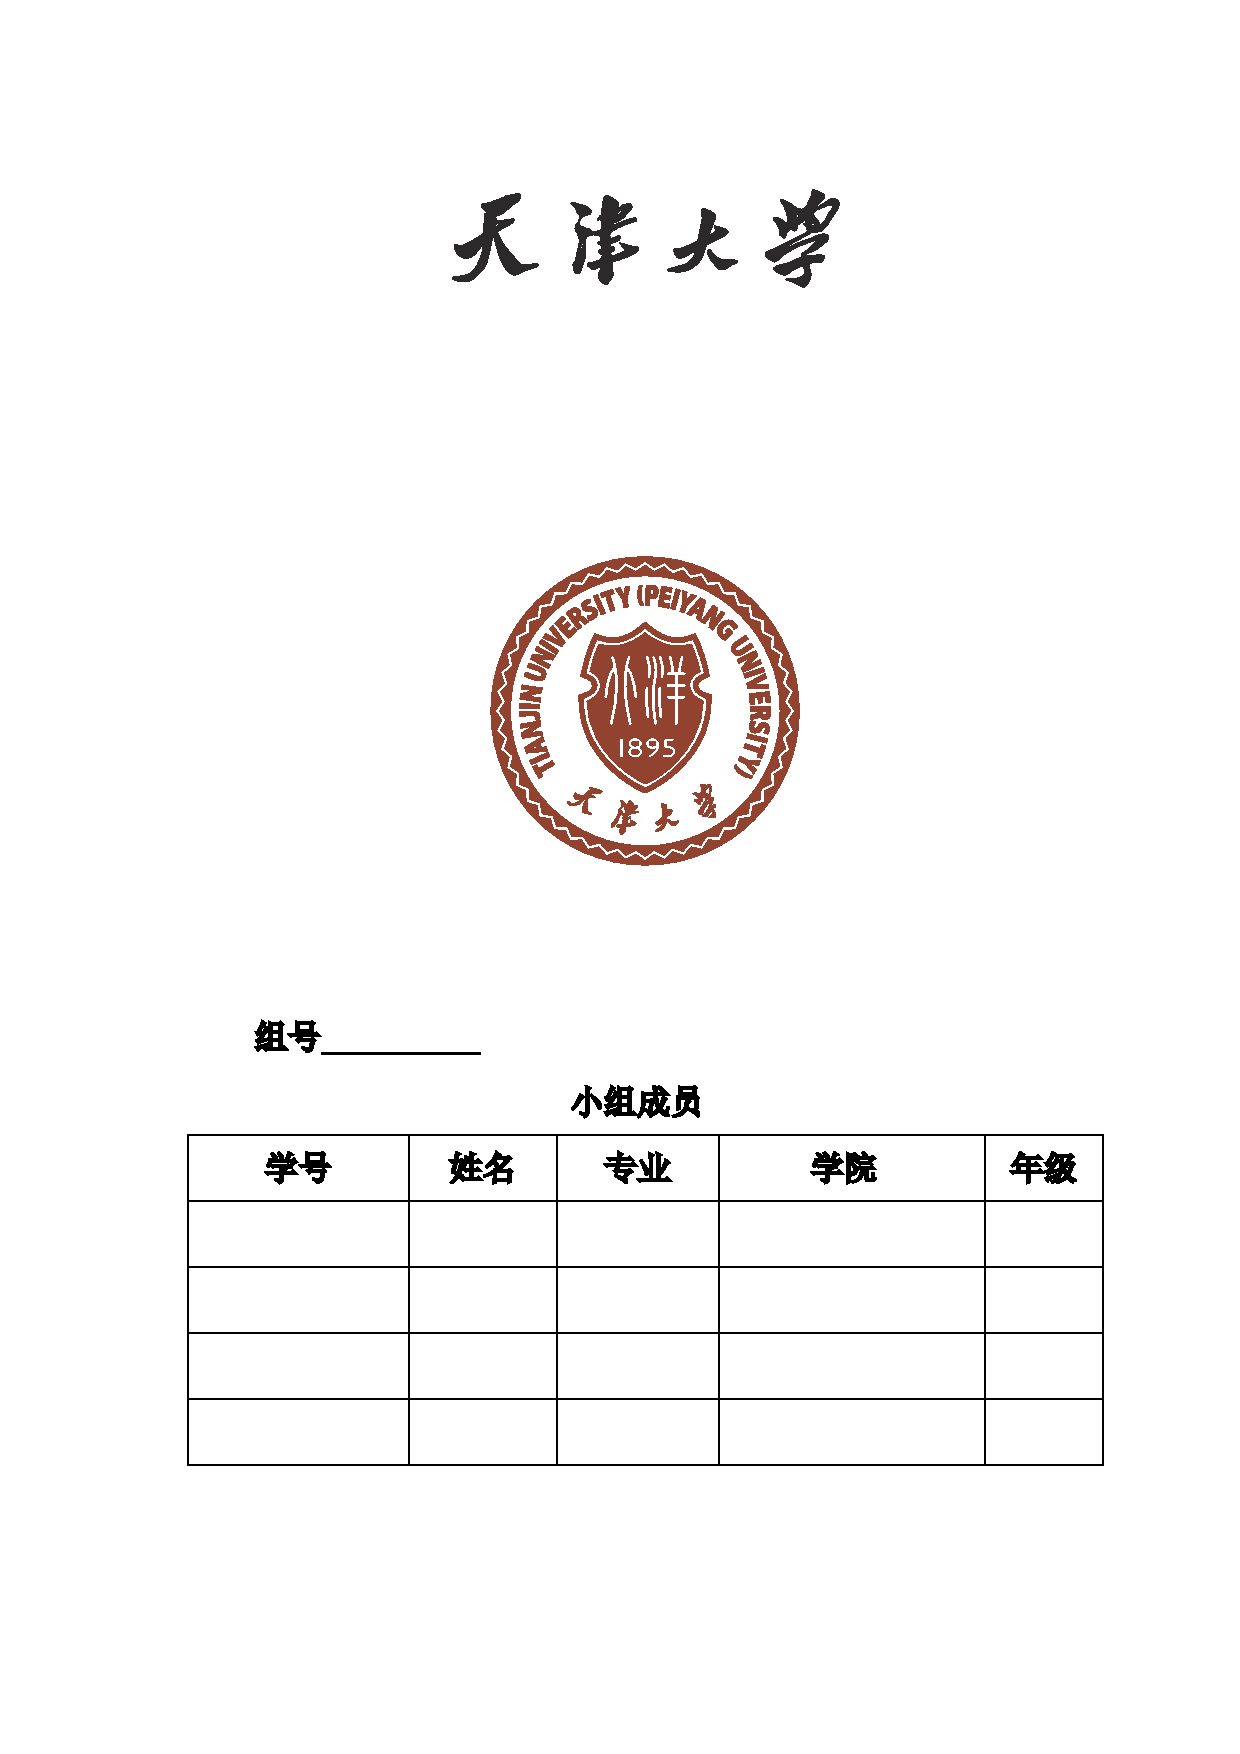
\includegraphics[width=\paperwidth,height=\paperheight]{figures/template/cover-background.pdf}}%
      \put(309.82,647){\makebox(0,0)[b]{\song\bfseries\fontsize{21bp}{25bp}\selectfont\@ccovertitle}}%
      \put(309.82,610){\makebox(0,0)[b]{\song\fontsize{15bp}{21bp}\selectfont\@cproject}}%
      \put(192.62,338){\makebox(0,0)[b]{\song\fontsize{14bp}{18bp}\selectfont\@ctitle}}%
      \membertable
      \put(395.26,83.7){\makebox(0,0)[b]{\song\bfseries\fontsize{16pt}{20pt}\selectfont 时间}}%
      \put(420,83.7){\makebox(0,0)[lb]{\song\fontsize{12bp}{15bp}\selectfont\@cdate}}%
    }}%
    \null
  \end{titlepage}
}

  \cheading{天津大学《软件工程 1》课程设计报告}
\ccovertitle{《软件工程 1》课程设计报告}
\ctitle{第十组}
\cproject{项目名称：轻量级外卖服务平台}
\caffil{软件学院}
\csubject{软件工程}
\cgrade{2024级}
\cauthor{范文丽、李承文、赵紫怡、仲禹潼}
\cstuid{3024244438、3024232129、3024244137、3024244140}
\newcommand{\membertable}{%
  \covermember{0}{3024244438}{范文丽}%
  \covermember{1}{3024232129}{李承文}%
  \covermember{2}{3024244137}{赵紫怡}%
  \covermember{3}{3024244140}{仲禹潼}%
}
\hypersetup{pdftitle={《软件工程 1》课程设计报告 - 轻量级外卖服务平台},pdfauthor={范文丽、李承文、赵紫怡、仲禹潼},pdfsubject={软件工程 1},pdfkeywords={软件工程, 敏捷开发, CMM3, AI赋能, 外卖平台}}
\cdate{2026~年~12~月}

  \frontmatter
  \hypersetup{pageanchor=false}
  \fancypagestyle{plain}{
    \fancyhf{}
    \renewcommand{\headrulewidth}{0pt}
    \fancyfoot[C]{\song\xiaowu~\thepage~}
  }

  \begingroup
    \renewcommand{\song}{\CJKfamily{coversong}}
    \renewcommand{\hei}{\CJKfamily{coverhei}}
    \makecover
  \endgroup
  % 单页目录列出七章及分类附录，页码由各章标签取得。
\clearpage
\begingroup
\pagestyle{empty}
\setcounter{page}{2}
\phantomsection
\pdfbookmark[0]{目录}{mulu}
\newcommand{\ReportTocRow}[3]{%
  \put(73.70,#1){\makebox(0,0)[lb]{\song\fontsize{12bp}{18bp}\selectfont
    \hbox to447.88bp{\hyperref[#2]{#3}\leaders\hbox to6bp{\hss.\hss}\hfill\pageref{#2}}}}%
}
\AddToShipoutPictureFG*{\AtPageLowerLeft{%
  \setlength{\unitlength}{1bp}%
  \put(297.64,745.92){\makebox(0,0)[b]{\song\bfseries\fontsize{18bp}{24bp}\selectfont 目录}}%
  \ReportTocRow{710}{sec:report-team}{一、团队建立}
  \ReportTocRow{686}{chap:definition}{二、定义项目}
  \ReportTocRow{662}{chap:process}{三、过程管理}
  \ReportTocRow{638}{chap:management}{四、项目管理}
  \ReportTocRow{614}{chap:delivery}{五、项目交付}
  \ReportTocRow{590}{chap:ai}{六、AI 赋能专题}
  \ReportTocRow{566}{chap:retrospective}{七、总结回顾}
  \ReportTocRow{528}{app:project}{附录A\quad 项目范围与工程基线}
  \ReportTocRow{504}{app:db}{附录B\quad 数据库表结构与迁移}
  \ReportTocRow{480}{app:api}{附录C\quad 接口契约与验证用例}
  \ReportTocRow{456}{app:tests}{附录D\quad 质量验证与部署配置}
  \ReportTocRow{432}{app:ui}{附录E\quad 界面路由与视觉规范}
  \ReportTocRow{408}{app:process}{附录F\quad 团队协作与迭代记录}
  \ReportTocRow{384}{app:ai}{附录G\quad AI 人工复核与演进事项}
}}
\null
\thispagestyle{empty}
\clearpage
\endgroup


  \mainmatter\hypersetup{pageanchor=true}\defaultfont\raggedbottom
  \tolerance=1800 \emergencystretch=1.8em
  \makeatletter
  \fancypagestyle{plain}{
    \fancyhf{}
    \fancyhead[C]{\song\wuhao \@cheading}
    \fancyfoot[C]{\song\xiaowu ~\thepage~}
    \renewcommand{\headrulewidth}{0.5pt}
    \renewcommand{\footrulewidth}{0pt}
  }
  \makeatother
  \setcounter{page}{1}

  \chapter{团队建立}\label{sec:report-team}

我们是天津大学软件学院 2024 级的四名本科生，共同完成了轻量级外卖服务平台的需求分析、设计、开发、测试和部署。小组按模块分工，联调时沿同一笔外送订单核对顾客、商家、骑手和管理员的操作衔接。项目代码托管在 GitHub 的 \texttt{lightweight-takeout-platform} 仓库。

\section{团队成员}

\paragraph{组长李承文（学号 3024232129）}
李承文担任项目经理和 Scrum Master，安排迭代、组织 PR 评审并负责部署。他维护 \code{elm_bk} 的认证、交易、资产、配送和管理端服务。后端使用 Java 17 和 Spring Boot 3.4.6，由 Spring Security 和 JWT 校验角色权限，通过 MyBatis 执行库存扣减和配送任务的条件更新。他还维护演示脚本和 \code{docker-compose.demo.yml}。

\paragraph{组员范文丽（学号 3024244438）}
范文丽负责顾客、商家和管理员的界面，代码位于 \mbox{\code{elmclient/src/views/}}。她维护 \mbox{\code{AiChat.vue}}、主题和数据看板。页面用 Vue 3 Composition API 管理状态，通过 Vue Router 限定各角色的页面入口，由 Axios 统一处理请求和异常。界面支持四套 CSS 变量主题、转场和窄屏适配，数据看板使用 ECharts/SVG 并支持 Excel/PDF 导出。

\paragraph{组员赵紫怡（学号 3024244137）}
赵紫怡兼任产品负责人，负责需求分析和数据库设计。她主编 \code{docs/SRS.pdf} 及飞书需求文档，用 UML 和 draw.io 描述各端用例，维护 MySQL 8 基线 \code{elm_bk/db/schema/elm_v2.sql} 与 \code{001}--\code{006} 迁移脚本。AI 点餐后端也由她负责。她维护 \mbox{\code{AiChatController}}、\mbox{\code{AssistantController}} 和多模态客户端，接入 DeepSeek 与 DashScope。

\paragraph{组员仲禹潼（学号 3024244140）}
仲禹潼负责质量保障和交叉验收，按等价类与边界值设计用例，通过 JUnit 5、MockMvc 和 Node 测试运行器复测，并在 WPS 台账登记缺陷。他负责地图功能，连接 \code{MapController}、\code{MapLocationPicker} 选址弹窗与 \code{RiderDashboard.vue} 的导航入口。选址使用 POI 检索和逆地理编码，骑手侧按 GCJ-02 坐标估算距离。

飞书保存需求与站会结论，涉及多个模块的决定在腾讯会议上讨论。GitHub 保留代码与评审意见，WPS 台账记录缺陷的复现步骤和复测结果。图~\ref{fig:team-topology} 列出了各项记录的维护人和成员之间的交接关系。

\begin{figure}[!htbp]
  \centering
  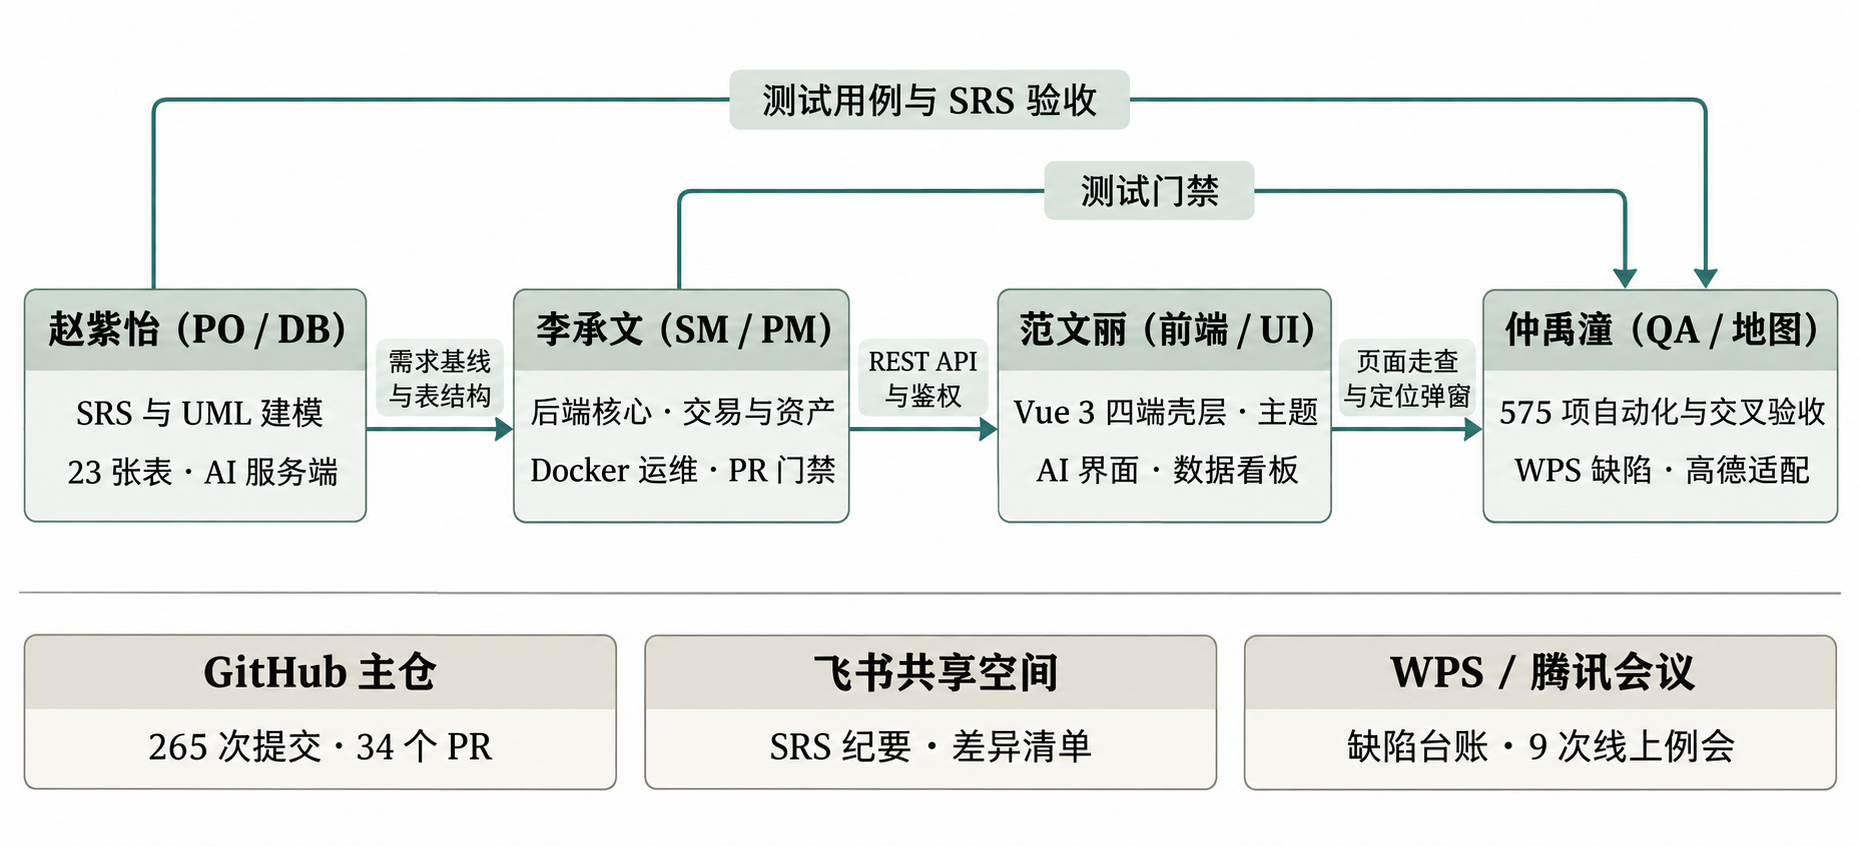
\includegraphics[width=.98\linewidth]{figures/report/process/team-handoff.png}
  \caption{小组成员角色分工与工程协作基础设施拓扑图}\label{fig:team-topology}
\end{figure}

店铺营业状态需要商家与顾客两端协作。需求约定\textbf{休息中的店铺保留菜单展示，暂停接收新订单}。商家提交后，后端保存状态并在加购和建单时检查，顾客端显示“休息中”。验收时用两个账号操作同一家店，分别核对商家保存的营业状态和顾客端的下单限制。

\section{团队角色与任务分配}

\subsection{需求、迭代与交付}

赵紫怡按 P0、P1 和 P2 将用例纳入 Product Backlog，在 SRS 中写明各角色的操作、异常处理和验收条件。团队评审系统上下文图、四端用例图、领域类图和状态机图时，把发现的状态命名差异记入飞书，在 SRS 2.0 中统一。迭代评审时，她再用需求里的用例检查已实现功能。

李承文将任务分到三个 Sprint，设置里程碑，组织站会、评审和回顾。前后端的字段或状态含义出现分歧时，他召集成员确认接口约定，再安排调整和联调。他负责主干保护、PR 评审和合并冲突处理，维护 \code{scripts/check-repository.mjs} 与容器演示环境，并在交付前核对风险台账、测试记录和部署材料。

\subsection{开发与联调}

四类角色各有页面入口，共用路由、主题及请求处理。范文丽负责页面组织和公共壳层，主要维护 \code{Index.vue}、\code{BusinessInfo.vue}、\code{Cart.vue}、\code{OrderList.vue}、\code{AiChat.vue}、\code{Preferences.vue} 以及商家和管理员看板。仲禹潼协作完成 \code{MapLocationPicker}、地址与地图联动，以及骑手工作台 \code{RiderDashboard.vue} 的导航入口。两人共同核对地址字段、\mbox{选址异常提示和窄屏布局}。

后端按 Controller、Service、Mapper 分层。李承文负责登录、角色切换和履约状态更新，也维护订单提交、计价、结算和资产服务，分别对应 \mbox{\code{OrderSubmissionService}}、\mbox{\code{OrderPricingService}}、\mbox{\code{OrderSettlementService}} 和 \mbox{\code{AssetService}}。订单提交、取消回滚、资产扣减和骑手接单都需要核对权限、幂等和事务边界。

赵紫怡维护对话和结构化助手服务，分别由 \mbox{\code{AiChatServiceImpl}} 和 \mbox{\code{StructuredAssistantServiceImpl}} 实现。她还维护 \mbox{\code{AiRecommendationServiceImpl}}，对接模型适配器和商家菜单查询。外部服务异常时，系统切回本地处理。

赵紫怡设计了 23 张核心业务表及主外键、查询索引，李承文协作处理迁移和并发更新。两人把成交时的商品、地址快照与商家的可变配置分开存储，维护订单、配送、资产流水、评价、通知和 AI 对话等表，并为账号唯一性、默认地址、菜品快照、备注和地图坐标编写版本化迁移。

\subsection{质量保障}

每轮功能完成后，仲禹潼先用四类账号检查页面和接口，再测试库存边界、密码、越权和定位异常。WPS 台账逐条记录缺陷所在模块、复现顺序、截图与复测结果。容易复发的问题写入自动化测试，开发者提交前运行，合并时由同伴复核。

回归中，后端 53 个 JUnit/MockMvc 测试类有 340 项通过，前端 28 个 Node 测试文件有 235 项通过。仲禹潼还组织人工走查与跨组交叉验收。表~\ref{tab:team-matrix} 列出成员分工和联调重点，附录表~\ref{tab:code-ownership} 记录主要代码与文档的归属。

\begin{longtable}{L{.09\linewidth}L{.155\linewidth}L{.24\linewidth}L{.455\linewidth}}
\caption{小组成员角色、扩展模块与协作接口矩阵}\label{tab:team-matrix}\\
\toprule
\textbf{成员} & \textbf{基础主责方向} & \textbf{Scrum/专项模块} & \textbf{协作接口与联调关注点} \\
\midrule
\endfirsthead
\multicolumn{4}{c}{{\tablename\ \thetable{} 续表}}\\
\toprule
\textbf{成员} & \textbf{基础主责方向} & \textbf{Scrum/专项模块} & \textbf{协作接口与联调关注点} \\
\midrule
\endhead
\bottomrule
\endfoot
范文丽 & 前端开发 & UI 主题、数据看板 & 对齐后端响应字段与页面状态，实现四端界面、主题切换与经营/平台看板可视化。 \\
李承文 & 后端开发 & 组长/SM、红包积分 & 统筹进度和 PR 合并，衔接订单定价、支付、优惠券、积分与钱包流水回退规则。 \\
赵紫怡 & 数据库设计 & PO/SRS、AI 点餐 & 主编 SRS 与数据模型，对接真实菜单、订单权限校验和多模态 AI 服务。 \\
仲禹潼 & 测试工程 & QA 负责人、高德地图 & 组织回归测试与交叉验收，验证地图选址、距离估算、骑手导航与降级场景。 \\
\end{longtable}

\section{培训大纲}

四人各有熟悉的方向，联调缺陷常同时涉及页面、服务和数据。培训先练习搭建环境、建分支和登记缺陷，要求每人在自己的电脑上走完一笔订单，再\mbox{按分工开展专题练习}。

\subsection{培训目标}

\begin{reportpoints}
\item 用 Scrum 组织迭代，结合课程讨论的需求管理、项目策划、验证和确认做法，对应 REQM、PP 和 VER/VAL。站会记录待处理事项，合入前审查代码，修复后按原步骤复测。
\item 每人能独立运行 Vue 3 前端、调试 Spring Boot 后端、初始化 MySQL 容器并执行测试。协作时统一使用 GitHub 特性分支和 PR，飞书与腾讯会议保存结论，WPS 台账登记缺陷，Playwright 和 Chrome 用于走查页面。
\item 选用服务端计价、JWT 身份读取、订单快照和外部服务超时练习 TDD。先用失败用例复现问题，再修改实现，最后用同一组用例保障整理后的代码行为。
\end{reportpoints}

\subsection{培训对象与分层重点}

全员先走读点餐至履约的四端流程，练习启动环境、认领任务、提交改动和归档。范文丽与仲禹潼随后练习路由守卫、CSS 变量主题、地图弹窗、响应式适配和前端单测。李承文与赵紫怡走读 MyBatis 映射，练习条件更新、事务回滚、\code{BigDecimal} 算价、历史快照和外部接口适配。仲禹潼与李承文把关键用例整理为可重复运行的回归测试，并练习 Nginx 代理与部署排查。分层安排见表~\ref{tab:training-roles}。

\subsection{培训内容与实施计划}

启动会上，李承文和赵紫怡通过腾讯会议讲解课程交付要求，演示如何从用户故事找到对应的图、接口和测试，并统一站会日志与缺陷登记字段。首轮开发前，范文丽示范 Vue 3 目录、Axios 拦截器和组件拆分，李承文讲解后端分层，赵紫怡带领组员阅读 \code{elm_v2.sql} 和迁移约定。李承文演示分支、PR 和 Docker Compose，仲禹潼检查组员能否在各自环境运行 \code{./mvnw test} 与 \code{npm test}。

交易规则训练以购物车多选结算、防超卖库存扣减和积分抵扣为例。赵紫怡和仲禹潼分别讲解 DeepSeek/DashScope 降级与高德坐标转换。测试训练将库存溢出、跨用户数据隔离整理成可重复执行的用例。联调中遇到异步竞态、返回循环和窄屏溢出时，组员开短会并一起查代码。早期演练的操作和检查条件见表~\ref{tab:training-labs}。

\begin{longtable}{L{.20\linewidth}L{.42\linewidth}L{.34\linewidth}}
\caption{团队工程实操演练与检查点}\label{tab:training-labs}\\
\toprule
\textbf{演练} & \textbf{操作} & \textbf{通过条件} \\
\midrule
Lab-01 环境联启 & 使用 \code{docker-compose.demo.yml}，或分别启动本地 MySQL、后端 Jar 与 Vue。再以 \code{demo_user}、\code{demo_merchant}、\code{demo_rider} 和 \code{demo_admin} 逐一登录。 & 四端首屏无控制台报错，接口返回 200，角色入口隔离。 \\
Lab-02 分支协作 & 从 \code{main} 创建特性分支，提交一项包含测试的变更，发起关联飞书任务的 PR。 & 提交信息规范，SM 复核通过，合入后无遗留冲突或\mbox{构建警告。} \\
Lab-03 角色权限 & 分别使用 Postman 或 MockMvc 验证无 Token 和跨账号的受保护请求。 & 请求返回相应的 401 或 403，服务端按 JWT 上下文\mbox{确认身份。} \\
Lab-04 \mbox{事务与快照} & 验证 \code{food} 表的条件库存更新。商家修改当前菜名后，查询 \code{orderdetailet} 中的\mbox{历史明细。} & 库存保持非负，历史订单的商品名称仍为成交时快照。 \\
Lab-05 缺陷回归 & 先写失败用例，再以最小改动使其通过，并把一次含截图的复现经过记入 \mbox{WPS 台账。} & 用例可以重复回归，台账可以追到修复记录与\mbox{复测结果。} \\
\bottomrule
\end{longtable}

\Needspace{.43\textheight}
\subsection{两类业务规则的实操}

角色权限练习从购物车开始。先以游客身份访问公开目录，再打开购物车，检查系统是否跳转到登录页。随后切换商家、骑手与管理员账号，访问各自的路由，并核对请求身份和返回数据的归属。

后端回归验证角色权限和数据归属。\code{CheckoutCartJourneyTest} 准备两位顾客、两家商铺和多条购物车记录，检查顾客只能查询自己的未删除条目，按商铺筛选时返回相应记录。未登录请求返回 401，前端和测试据此区分空购物车与 \mbox{登录失效}。

事务练习用一笔订单串起菜品、库存和明细。提交前读取当前商品，保存订单时将菜名、单价及数量写入明细。商家修改商品后，顾客与商家分别打开历史订单，核对成交快照。新订单使用更新后的菜单和单价。对照两笔订单，可以定位问题发生在建单写入还是历史查询。

权限练习用 MockMvc 发送请求，订单快照用例在独立的 H2 测试库运行。测试类保留初始数据和断言，失败时可检查写入字段与查询来源。交付时，团队在独立演示实例上走查四端，将界面、接口响应和自动化结果对照。联调与回归均可重复这套步骤。

结算由前后端联合检查。顾客修改地址后返回结算页，\code{checkout.test.mjs} 验证原店铺、菜品和履约方式仍在。切换自取时，前端省略收货地址，服务端将配送费计为零并跳过起送价检查。商品丢失时先查页面回填，自取被起送价拦住时检查后端计价分支。

\subsection{培训考核与验收标准}

每位成员都要拉取仓库、执行 \code{ensure-demo-env.sh}、启动环境并完成至少一次分支和 PR 操作。前端实操检查角色路由与接口，后端和数据库至少提交一组带条件更新的 Mapper 查询及单测，测试人员提交涵盖正常流程和异常边界的用例清单。首轮结束时，团队对照飞书任务、GitHub 提交和测试结果验收，并登记重大接口变更。\mbox{量化结果见表~\ref{tab:training-eval}}。

  \chapter{定义项目}

本章围绕“轻量级外卖服务平台”开展项目范围定义与软件系统设计，覆盖产品愿景与敏捷规划、MoSCoW 优先级与 Product Backlog、技术架构、MySQL 8 数据库模型（全量 23 张数据表）、四端及特色功能详细设计、RESTful 接口契约（全量 24 个控制器 135 个端点）与用户界面（UI）设计。

\section{产品愿景与敏捷规划}

\subsection{背景与目的}

\subsubsection{项目背景}
在高校校园及周边生活场景中，师生点餐需求高频且集中，但传统校园订餐方式仍存在流程割裂、履约不透明及扩展能力有限等痛点：
\begin{enumerate}
  \item \textbf{订单与履约流转非标准化：} 人工记录、微信接龙或电话沟通容易出现地址漏填、菜品规格误记、起送门槛判断错误及到店自取与外送混淆等问题，缺乏可追踪的状态机约束。
  \item \textbf{多方角色权责边界不清：} 商家缺少对商品上下架、库存、满减活动及营业状态的自主管控；骑手缺乏统一的抢单、到店、取餐与异常上报工作台；管理员缺少准入审核与平台级治理视图。
  \item \textbf{消费决策与交互体验割裂：} 顾客缺少基于个人口味忌口的智能推荐入口，难以在下单前透明核对“满减、会员折扣、优惠券、积分抵扣”的真实计算顺序，历史订单也常因商家改价或下架商品而发生信息漂移。
  \item \textbf{并发安全与系统可靠性不足：} 高峰期多用户抢购有限库存、重复点击支付以及多名骑手同时抢同一配送任务时，若缺少条件更新、幂等键与事务保护，极易引发超卖、重复扣款或任务归属冲突。
\end{enumerate}

\subsubsection{项目核心目标（与 TQCS 对齐）}
围绕软件工程时间（Time）、质量（Quality）、成本（Cost）与范围（Scope）控制目标，本项目在课程初始工程基础上完成架构重构与全链路增强（详见表~\ref{tab:tqcs-goals}）：
\begin{enumerate}
  \item \textbf{构建四端闭环（Scope \& Quality）：} 打通顾客、商家、骑手、管理员四端核心流程，支持外送与到店自取双模式，实现订单状态与配送任务的严格联动。
  \item \textbf{强化数据与资金准确性（Reliability）：} 采用服务端权威计价、下单商品/地址快照隔离、条件更新防超卖及幂等支付机制，保障交易记录与资产流水准确可追溯。
  \item \textbf{融入 AI 与地图差异化能力（Innovation）：} 提供文字对话、智能推荐、图片识菜、语音草稿四类受控 AI 点餐入口，结合高德地图实现精准选址、直线距离与送达时长估算。
  \item \textbf{按敏捷迭代按期交付（Time \& Cost）：} 遵循 Scrum + CMM3 过程规范，通过三大短周期迭代及持续自动化测试保护，在有限周期内高质量完成交付与验收。
\end{enumerate}

\begin{longtable}{L{.14\linewidth}L{.26\linewidth}L{.51\linewidth}}
\caption{项目 TQCS 工程目标与量化验收基准表}\label{tab:tqcs-goals}\\
\toprule
\textbf{TQCS 维度} & \textbf{核心管理目标} & \textbf{量化验收标准} \\
\midrule
\endfirsthead
\multicolumn{3}{c}{{\tablename\ \thetable{} 续表}}\\
\toprule
\textbf{TQCS 维度} & \textbf{核心管理目标} & \textbf{量化验收标准} \\
\midrule
\endhead
\bottomrule
\endfoot
Time（进度） & 三大 Scrum 短周期迭代按期收敛 & 9 月 1 日至 9 月 19 日完成全部 P0/P1 主流程与扩展功能，核心演示版本准时封板。 \\
Quality（质量） & 高覆盖自动化回归与零高危越权缺陷 & 后端 53 个测试类（340 项）与前端 28 个测试文件（235 项）100\% 通过，高危越权与并发问题清零。 \\
Cost（成本） & 4 人跨职能协同与外部依赖可控降级 & 总实际工时控制在 238~h（偏差 +3.48\%），未配置外部 AI/地图密钥时基础主链路零成本阻塞。 \\
Scope（范围） & 聚焦四端闭环与特色增值能力 & 严格执行 MoSCoW 分级，将真实支付清算与高频 GPS 轨迹明确划出本期基线，防止范围蔓延。 \\
\end{longtable}

\subsection{项目定义}

\subsubsection{项目名称}
轻量级外卖服务平台（课程演进代号：饿了吧校园外卖平台）。

\subsubsection{核心功能定位与目标用户}
\begin{enumerate}
  \item \textbf{顾客端（校园及周边消费者）：} 支持游客与登录态浏览、分类搜索、口味偏好与主题切换、高德地图选址与收货地址管理、购物车跨店隔离与部分勾选提交、外送/自取切换、服务端算价与模拟钱包/积分/优惠券支付、订单全流程跟踪与取消、评价发布、收藏点赞及 AI 辅助点餐。
  \item \textbf{商家端（校内食堂档口及周边餐饮商户）：} 支持入驻申请与审核状态查看、店铺资料与满减/营业状态配置、菜品分类/价格/库存/限购与上下架管理、订单接单/拒单/出餐流转、顾客评价查看与回复，以及经营数据看板与报表导出。
  \item \textbf{骑手端（校园兼职或专职配送员）：} 支持实名与车辆类型入驻申请、在线/离线状态切换、可接配送任务抢单、到店确认、取餐配送、确认送达、异常情况上报，以及高德外部导航联动与收益里程统计。
  \item \textbf{管理员端（平台运营与治理人员）：} 支持商家/开店/骑手准入审核、用户与商家账号治理（启用/停用/角色分配）、配送异常人工处置（恢复/改派/终止）、评价隐藏治理以及平台级交易趋势看板。
\end{enumerate}

\subsection{迭代周期与 Scrum 机制}

团队采用增量式 Scrum 敏捷开发框架，并结合 CMM3 级过程域实施标准化管理：
\begin{itemize}
  \item \textbf{迭代周期划分：} 核心研发工作划分为 3 个紧凑迭代周期（Sprint 1：需求建模与用户下单核心闭环；Sprint 2：商家履约、骑手配送与资产体系；Sprint 3：管理治理、AI 多模态、高德地图与全链路回归），随后开展跨组交叉验收与《软件工程 1》规范化文档归档。
  \item \textbf{敏捷例会制度：} 每个迭代起点召开规划会拆解 Sprint Backlog；开发期间通过飞书文档与线上短会同步每日进展与阻塞；迭代末期开展演示评审与问题回顾，并依据 TDD 红--绿--重构与自动化测试门禁合并 PR。
  \item \textbf{就绪与完成定义（DoR / DoD）：} 团队明确规定只有具备明确角色故事、接口字段与异常边界的用户故事才允许进入 Sprint（DoR）；只有完成编码实现、通过前后端自动化测试、经过 SM 代码审查合并且飞书状态更新的任务才标记为完成（DoD），具体准则见表~\ref{tab:dor-dod}。
\end{itemize}

\begin{longtable}{L{.18\linewidth}L{.35\linewidth}L{.38\linewidth}}
\caption{团队敏捷就绪定义（DoR）与完成定义（DoD）检查标准}\label{tab:dor-dod}\\
\toprule
\textbf{质量门禁阶段} & \textbf{核心准入/验收条目} & \textbf{工程验证载体} \\
\midrule
\endfirsthead
\multicolumn{3}{c}{{\tablename\ \thetable{} 续表}}\\
\toprule
\textbf{质量门禁阶段} & \textbf{核心准入/验收条目} & \textbf{工程验证载体} \\
\midrule
\endhead
\bottomrule
\endfoot
DoR（迭代就绪） & 1. 故事具备明确的角色、目标、商业价值及 MoSCoW 优先级；\newline 2. 涉及表结构变更已明确迁移 SQL 策略；\newline 3. 前后端已对齐请求路径、DTO 字段与状态码。 & 飞书 Product Backlog、SRS 用例章节与 \code{elm_v2.sql} 评审记录 \\
\midrule
DoD（任务完成） & 1. 核心逻辑与分支边界通过 \code{./mvnw test} 与 \code{npm test}；\newline 2. 安全边界（JWT 上下文提取、权限注解）经人工复核；\newline 3. PR 合并至 \code{main} 且未破坏容器一键启动脚本；\newline 4. 关联缺陷已在 WPS 台账复测关闭。 & GitHub PR 合并记录、Surefire/Node 测试日志、WPS 闭环台账 \\
\end{longtable}

\section{项目范围与 Product Backlog}

\subsection{项目范围界定}

图~\ref{fig:def-context} 与图~\ref{fig:def-actors} 分别展示了系统的上下文外部依赖边界与四类参与者职责。平台内部由前端 SPA、Spring Boot 业务服务与 MySQL 8 持久化层构成；外部依赖包括 DeepSeek 大模型、DashScope 视觉与语音识别、高德地图服务及对象存储。本期明确将范围边界固化在表~\ref{tab:scope-boundary} 中，避免需求蔓延挤压测试回归窗口。

\begin{longtable}{L{.16\linewidth}L{.38\linewidth}L{.37\linewidth}}
\caption{系统建设范围（In-Scope）与显式排除项（Out-of-Scope）清单}\label{tab:scope-boundary}\\
\toprule
\textbf{范围分类} & \textbf{本期纳入建设范围（In-Scope）} & \textbf{显式排除项与理由（Out-of-Scope）} \\
\midrule
\endfirsthead
\multicolumn{3}{c}{{\tablename\ \thetable{} 续表}}\\
\toprule
\textbf{范围分类} & \textbf{本期纳入建设范围（In-Scope）} & \textbf{显式排除项与理由（Out-of-Scope）} \\
\midrule
\endhead
\bottomrule
\endfoot
认证与权限域 & 统一账号注册/登录、BCrypt 加密、JWT 无状态鉴权、商家/骑手入驻审批与角色路由隔离 & 第三方微信/QQ OAuth 授权登录、短信真实验证码付费通道（演示环境保留本地校验） \\
顾客点餐域 & 分类搜索、店铺详情、限购与库存校验、跨店购物车、外送/自取双模结算、订单跟踪与评价 & 跨商家合并拆单支付、拼单外卖、复杂预售定时排期 \\
资金与资产域 & 服务端权威算价、模拟钱包充值、模拟支付、新人/领券核销、积分累计与抵扣、只增不改流水账本 & 真实微信支付/支付宝商户号清算、银行卡提现打款与发票税控 \\
配送与地图域 & 骑手入驻审核、在线接单池、乐观锁并发抢单、到店/取餐/送达、异常仲裁、高德选址与距离估算 & 商业级智能路径派单调度算法、骑手实时高频 WebSocket GPS 轨迹推流 \\
智能与管理域 & 结构化菜单筛选、DeepSeek 问答、DashScope 识菜与语音草稿（含未配置降级）、四端看板与导出 & 大规模向量知识库 RAG 集群、单用户精细化商业计费配额系统 \\
\end{longtable}

\srsfig[0.95\linewidth]{figures/srs/01-system-context.png}{系统上下文边界与外部依赖集成视图}{fig:def-context}

\srsfig[0.92\linewidth]{figures/srs/09-actor-analysis.png}{系统四端参与者职责与交互边界分析模型}{fig:def-actors}

\subsection{Product Backlog}

本组结合 MoSCoW 优先级法则（P0：必须实现的核心基线；P1：应当实现的完整增强；P2：条件允许时纳入的可选增强），并对照《软件需求规格说明书》（SRS）中的标准用例编号（\code{UC-COM/CUS/MER/RID/ADM/AI/MKT/PER}），将全部需求拆解为 22 项标准用户故事（\code{US001}--\code{US022}，总故事点 118 点），构成项目的 Product Backlog。表~\ref{tab:backlog-summary} 汇总了优先级分布，表~\ref{tab:product-backlog} 给出了完整的用户故事卡片与验收标准。

\begin{longtable}{C{.14\linewidth}L{.28\linewidth}C{.16\linewidth}C{.16\linewidth}L{.18\linewidth}}
\caption{Product Backlog 优先级与故事点统计表}\label{tab:backlog-summary}\\
\toprule
\textbf{优先级} & \textbf{MoSCoW 业务定位} & \textbf{故事数量} & \textbf{故事点合计} & \textbf{主要覆盖迭代} \\
\midrule
P0（Must） & 核心交易、四端履约与安全闭环（MVP 基线） & 14 项 & 78 点（66.1\%） & Sprint 1 -- Sprint 2 \\
P1（Should） & 资产优惠、评价通知、看板与结构化智能服务 & 6 项 & 31 点（26.3\%） & Sprint 2 -- Sprint 3 \\
P2（Could） & 多模态识菜/语音草稿、高德定位与视觉动效增强 & 2 项 & 9 点（7.6\%） & Sprint 3 \\
\midrule
\textbf{合计} & \textbf{全平台四端及特色扩展需求} & \textbf{22 项} & \textbf{118 点（100\%）} & \textbf{Sprint 1 -- Sprint 3} \\
\bottomrule
\end{longtable}

\begin{longtable}{L{.08\linewidth}L{.10\linewidth}L{.11\linewidth}L{.34\linewidth}C{.06\linewidth}C{.06\linewidth}L{.17\linewidth}}
\caption{Product Backlog 详细用户故事与验收标准清单（US001--US022）}\label{tab:product-backlog}\\
\toprule
\textbf{编号} & \textbf{SRS 映射} & \textbf{角色} & \textbf{用户故事描述（As a / I want / So that）} & \textbf{优先} & \textbf{点数} & \textbf{核心验收标准（DoD）} \\
\midrule
\endfirsthead
\multicolumn{7}{c}{{\tablename\ \thetable{} 续表}}\\
\toprule
\textbf{编号} & \textbf{SRS 映射} & \textbf{角色} & \textbf{用户故事描述（As a / I want / So that）} & \textbf{优先} & \textbf{点数} & \textbf{核心验收标准（DoD）} \\
\midrule
\endhead
\bottomrule
\endfoot
US001 & UC-COM-01 & 通用用户 & 作为平台用户，我希望能通过账号密码注册、登录、修改个人资料/头像并安全退出，以便使用受保护功能。 & P0 & 5 & 用户名/手机号全局唯一；错误密码与停用账号拒绝登录；JWT 无状态鉴权且密码密文不回传。 \\
US002 & UC-COM-02/03 & 通用用户 & 作为已登录用户，我希望能申请成为商家或骑手并查看站内审核通知，以便合法切换对应工作端。 & P0 & 5 & 角色切换严格由服务端权威权限决定；入驻审核结果实时写入站内通知并支持标为已读。 \\
US003 & UC-CUS-01 & 游客/顾客 & 作为游客或顾客，我希望能按分类、关键字、销量或起送价浏览店铺及菜品详情，以便快速决策选餐。 & P0 & 5 & 未登录可公开浏览店铺，休息中店铺明确标示并拦截加购；售罄/下架菜品不可下单。 \\
US004 & UC-COM-02 & 顾客 & 作为顾客，我希望能增删改查收货地址并设置默认地址，以便下单结算时自动填充联系信息。 & P0 & 3 & 仅本人可读写本人地址；支持 11 位有效手机号正则校验与默认地址唯一切换。 \\
US005 & UC-CUS-02 & 顾客 & 作为顾客，我希望能分店管理购物车、填写口味备注并支持部分勾选商品结算，以便灵活安排多人点餐。 & P0 & 8 & 同商品自动合并数量；超限购/超库存拦截；未勾选商品提交后仍保留在购物车中。 \\
US006 & UC-CUS-03/04 & 顾客 & 作为顾客，我希望能选择外送或到店自取模式进行试算并幂等提交订单，以便准确完成下单支付。 & P0 & 8 & 自取免外送费、起送价及收货地址；按 \code{idempotencyKey} 防重复建单；高并发防超卖。 \\
US007 & UC-CUS-04/05 & 顾客 & 作为顾客，我希望能查看本人订单状态时间线、取消未接单订单并确认收货，以便掌控交易闭环。 & P0 & 5 & 跨用户订单严格隔离（403）；取消订单事务内恢复库存与退还资产；确认收货发放积分。 \\
US008 & UC-CUS-06 & 顾客 & 作为顾客，我希望能对已完成订单进行 1--5 星评价（支持传图）、查看商家回复以及点赞收藏店铺。 & P1 & 5 & 坚持“一单一评”原则；支持上传最多 3 张评价图片；收藏列表支持增删查看。 \\
US009 & UC-MKT-01 & 顾客 & 作为顾客，我希望能使用模拟钱包充值、领取新人券、开通 30 天体验会员及用积分抵扣订单金额。 & P1 & 8 & 所有金额严格采用 \code{BigDecimal} 精确运算；钱包扣款、退款与积分变更均记入流水账本。 \\
US010 & UC-PER-01 & 顾客 & 作为顾客，我希望能切换 4 套视觉主题并保存辣度、口味偏好与忌口标签，以便获得个性化界面与推荐。 & P1 & 3 & 主题切换即时应用 CSS 变量并同步后端；支持一键恢复默认设置且屏蔽过敏忌口提示。 \\
US011 & UC-MER-01 & 商家 & 作为商家，我希望能提交开店申请并维护店名、地址、起送费、配送费、满减规则及营业/休息状态。 & P0 & 5 & 仅审核通过的本人店铺可维护营业配置；切换“休息中”后顾客端同步禁止新下单。 \\
US012 & UC-MER-02 & 商家 & 作为商家，我希望能新增/编辑菜品、自定义菜品分类、调整库存与单笔限购并控制上下架状态。 & P0 & 5 & 修改商品名或价格不影响历史订单明细快照（\code{food_name_snapshot}）；库存支持原子条件扣减。 \\
US013 & UC-MER-03 & 商家 & 作为商家，我希望能查看本店待处理与进行中订单明细，并执行接单、拒单退款或确认出餐操作。 & P0 & 5 & 拒单自动退还顾客资产与恢复库存；出餐后外送订单自动生成待抢配送任务，自取转为待取餐。 \\
US014 & UC-MER-04 & 商家 & 作为商家，我希望能查看顾客评价并发布回复，并在经营看板按日期范围查看营收与热销趋势、导出报表。 & P1 & 5 & 仅本店所属订单评价可回复；经营看板支持 CSV/Excel 导出且数据与真实已完成订单一致。 \\
US015 & UC-RID-01/02 & 骑手 & 作为骑手，我希望能提交实名与车辆类型入驻申请，审核通过后切换在线接单并在任务池抢单。 & P0 & 5 & 采用乐观锁（\code{version}）条件更新实现并发抢单互斥，后发起请求明确返回“任务已被领取”。 \\
US016 & UC-RID-03/04 & 骑手 & 作为骑手，我希望能按“到店 $\rightarrow$ 取餐 $\rightarrow$ 送达”节点推进配送，并使用高德地图外部导航。 & P0 & 5 & 节点推进同步主订单状态并记录时间戳；缺坐标时自动降级为文本地址提示而不阻断履约。 \\
US017 & UC-ADM-01 & 管理员 & 作为管理员，我希望能集中审核商家入驻、新店铺开店及骑手资格申请，控制平台准入质量。 & P0 & 5 & 审核通过或拒绝必须记录审批意见并自动触发站内通知；未授权账号访问返回 403。 \\
US018 & UC-ADM-02 & 管理员 & 作为管理员，我希望能启停违规用户账号、隐藏恶意评价并查看平台汇总订单，维护社区生态。 & P0 & 5 & 停用账号立即拦截登录与接口调用；隐藏评价在公开店铺页不可见但保留后台审计记录。 \\
US019 & UC-AI-01 & 顾客 & 作为顾客，我希望能通过 AI 客服咨询平台规则与个人订单状态，并通过条件推荐获得真实菜品候选卡片。 & P1 & 5 & AI 不得直接代下单；候选菜品必须来自在售库存表且支持一键加购；订单查询严格隔离本人数据。 \\
US020 & UC-AI-02 & 顾客 & 作为顾客，我希望能上传菜品图片识菜或通过语音生成点餐草稿，并在未配置模型时获得清晰提示。 & P2 & 5 & 外部网络调用置于数据库事务外；超时熔断后平滑降级至本地筛选规则，绝不阻断普通点餐。 \\
US021 & UC-RID-04 / ADM-02 & 骑手/管理员 & 作为骑手我希望能上报配送异常，作为管理员我希望能对异常任务执行恢复、改派或终止仲裁。 & P0 & 4 & 异常上报同步挂起主订单（状态 9）；管理员仲裁恢复原态、换绑骑手或取消订单并回退资产。 \\
US022 & UC-ADM-03 / CUS-06 & 管理员/顾客 & 作为管理员我希望能查看平台级多维趋势看板与导出数据，作为顾客我希望能按月/年查看个人消费统计。 & P1 & 4 & 平台看板支持按时间粒度统计成交额、活跃店铺与订单分布；消费统计支持按月/年维度聚合展示。 \\
\end{longtable}

\section{技术架构与风险应对}

\subsection{技术栈选型}

平台采用前后端完全分离的现代 Web 架构，总体技术架构见图~\ref{fig:def-arch}。为保证大型单页应用的加载效率，前端仅首页保留首屏同步打包，商家端、骑手端、管理员端及 AI 点餐页均采用路由懒加载；后端采用经典的 \textbf{Controller $\rightarrow$ Service $\rightarrow$ Mapper（MyBatis）$\rightarrow$ MySQL 8} 分层架构，并将第三方外部依赖（DeepSeek、DashScope、高德地图）封装为独立客户端与适配器层，严禁与数据库事务耦合。系统各层技术选型及工程用途见表~\ref{tab:tech-stack}。

\srsfig[0.95\linewidth]{figures/report/process/architecture.png}{轻量级外卖服务平台五层技术架构与外部服务解耦视图}{fig:def-arch}

在代码组织层面，系统严格划分以下五层职责边界：
\begin{enumerate}
  \item \textbf{表现与交互层（\code{elmclient/src/views/} 与 \code{components/}）：} 基于 Vue 3 Composition API 与全局 CSS 变量主题引擎构建 33 个页面视图，配合 \code{authGuard.js} 实施四端角色路由隔离。
  \item \textbf{前端通信与状态契约层（\code{elmclient/src/services/} 与 \code{utils/}）：} 通过 Axios 拦截器统一注入 Bearer JWT 并拦截跨站泄露；封装 \code{checkout.js}、\code{amap.js}、\code{theme.js} 等纯函数工具以支持 Node 无浏览器单元测试。
  \item \textbf{安全网关与接口控制器层（\code{elm_bk/config/} 与 \code{controller/}）：} Spring Security 过滤器链解析并校验 JWT，配合 \code{@PreAuthorize} 注解与 \code{CurrentUserService} 从认证上下文提取真实用户身份；\code{GlobalExceptionHandler} 将业务异常映射为标准 HTTP 401/403/404/409/422/503 状态码。
  \item \textbf{核心业务与事务服务层（\code{elm_bk/service/impl/}）：} 承载订单权威计价（\code{OrderPricingService}）、混合资产结算（\code{OrderSettlementService}）、订单状态机及骑手乐观锁抢单等核心逻辑，确保资金与库存操作处于 ACID 事务边界内。
  \item \textbf{持久层与外部隔离适配层（\code{mapper/} 与 \code{client/}）：} MyBatis 显式 XML/注解 SQL 控制复杂条件更新与历史快照写入；DeepSeek、DashScope 与高德 REST 客户端均配置独立超时控制与 \code{AiCircuitBreaker} 熔断器，故障时自动回退本地规则。
\end{enumerate}

\begin{longtable}{L{.18\linewidth}L{.28\linewidth}L{.45\linewidth}}
\caption{系统技术栈选型与工程用途}\label{tab:tech-stack}\\
\toprule
\textbf{架构层级} & \textbf{核心技术与版本} & \textbf{选型依据与工程用途} \\
\midrule
\endfirsthead
\multicolumn{3}{c}{{\tablename\ \thetable{} 续表}}\\
\toprule
\textbf{架构层级} & \textbf{核心技术与版本} & \textbf{选型依据与工程用途} \\
\midrule
\endhead
\bottomrule
\endfoot
前端工程 & Vue 3 + Vue Router 4 + Axios + CSS Variables & 组合式 API 便于拆分业务逻辑；路由元信息实现四端权限守卫；CSS 变量实现 4 套主题即时切换。 \\
前端质量与构建 & Vue CLI + Node.js Test Runner (\code{node --test}) & 零额外重型框架即可执行 28 个测试文件（235 项断言），保障算价、导航与契约回归。 \\
后端应用框架 & Java 17 + Spring Boot 3.4.6 + Spring Security & 提供稳健的 REST 接口、方法级权限控制（\code{@PreAuthorize}）、参数校验与全局异常处理。 \\
认证与实时推送 & JJWT (HMAC-SHA512) + WebSocket & 无状态令牌鉴权（含记住我时长区分）与订单状态实时推送通道。 \\
数据持久化 & MySQL 8.0 + MyBatis + HikariCP + 迁移脚本 & MyBatis 便于精准编写条件更新 SQL 与历史快照写入；版本号递增脚本保障可复现演进。 \\
外部服务适配 & DeepSeek API + DashScope + 高德 Web/JS API & 接入大模型对话、多模态识菜/语音识别与地理编码；内置超时限制、熔断器与降级路径。 \\
后端测试与容器 & JUnit 5 + Mockito + MockMvc + H2 + Docker Compose & H2 内存库支撑 53 个测试类（340 项）秒级隔离执行；Docker Compose + Nginx 一键编排交付。 \\
\end{longtable}

\subsection{初期架构风险与敏捷应对}

在架构设计初期，团队重点识别了多端共用后端、资金并发一致性及外部依赖稳定性三类高风险架构决策点，并制定了敏捷演进对策（见表~\ref{tab:init-risk}）。

\begin{longtable}{L{.22\linewidth}L{.33\linewidth}L{.36\linewidth}}
\caption{项目定义阶段核心技术风险与敏捷应对}\label{tab:init-risk}\\
\toprule
\textbf{初期架构风险点} & \textbf{潜在系统故障后果} & \textbf{架构层敏捷应对策略} \\
\midrule
\endfirsthead
\multicolumn{3}{c}{{\tablename\ \thetable{} 续表}}\\
\toprule
\textbf{初期架构风险点} & \textbf{潜在系统故障后果} & \textbf{架构层敏捷应对策略} \\
\midrule
\endhead
\bottomrule
\endfoot
信任客户端价格与身份参数 & 恶意篡改下单金额或伪造 \code{userId}/\code{riderId} 越权读写他人订单 & 彻底废弃客户端金额直传；后端从 JWT 上下文提取身份并重新查库计算全部价格。 \\
外部 AI 调用嵌入数据库事务 & 大模型慢响应（3--10 秒）长期占用数据库连接池导致系统雪崩 & 在 \code{AiChatServiceImpl} 与 \code{StructuredAssistantServiceImpl} 中先完成外部调用，再开启短事务落库。 \\
高并发库存扣减与骑手抢单冲突 & 热门商品超卖为负库存、多个骑手同时抢单造成任务归属错乱 & 采用 \code{stock >= qty} 条件更新扣库存，为 \code{delivery_task} 引入 \code{version} 乐观锁校验。 \\
多端演进导致旧前端接口失配 & 保留的课程初始接口与新增 v1 业务接口返回数据结构不一致 & 在旧 Controller 内保留兼容路径并统一委托至同一 Service，同时编写接口契约清理测试守护。 \\
第三方地图或密钥未配置阻断演示 & 课程部署环境缺少高德或 DashScope 密钥时，选址或点餐页面卡死报错 & 地图选址增加离线地址回退与“距离暂无”提示；AI 服务不可用时自动切换本地筛选帮助。 \\
\end{longtable}

\section{数据库设计}

\subsection{数据库概述}

系统数据库基于 MySQL 8.0（字符集统一为 \code{utf8mb4}、排序规则 \code{utf8mb4_0900_ai_ci}、存储引擎 InnoDB）构建，整体设计严格遵循第三范式（3NF）以消除基础实体冗余；同时针对外卖交易场景特有的“历史不可变性”需求，在订单明细与收货地址中引入受控的反范式快照字段（\code{food_name_snapshot}、\code{food_price} 与 \code{address_snapshot}），确保商家后续改价、改名或下架商品不会污染既有历史账单。

\subsection{领域模型与数据表设计}

图~\ref{fig:def-domain-core} 与图~\ref{fig:def-domain-assets} 分别展示了系统核心交易领域（用户、店铺、商品、购物车、订单、配送）与扩展增值领域（资产流水、优惠券、偏好、AI 会话）的 UML 类图模型。全库共包含 23 张数据表，按五大业务域汇总于表~\ref{tab:db-overview}。

\srsfig[0.96\linewidth]{figures/srs/02-core-domain-class.png}{系统核心交易与多端履约领域模型类图}{fig:def-domain-core}

\srsfig[0.94\linewidth]{figures/srs/03-assets-preference-class.png}{用户资产、优惠券、偏好与 AI 会话领域模型类图}{fig:def-domain-assets}

\begin{longtable}{L{.18\linewidth}L{.31\linewidth}L{.42\linewidth}}
\caption{系统 23 张数据库表全景清单}\label{tab:db-overview}\\
\toprule
\textbf{业务域} & \textbf{数据表名} & \textbf{核心业务职责} \\
\midrule
\endfirsthead
\multicolumn{3}{c}{{\tablename\ \thetable{} 续表}}\\
\toprule
\textbf{业务域} & \textbf{数据表名} & \textbf{核心业务职责} \\
\midrule
\endhead
\bottomrule
\endfoot
认证与用户域 & \code{users}、\code{person}、\code{authority}、\code{user_authority}、\code{permission_application} & 账号密码、个人基础资料（手机号唯一）、角色字典、多角色授权关联与商家入驻申请审核。 \\
店铺与商品域 & \code{business}、\code{food}、\code{merchant_interaction} & 店铺基本信息、满减门槛、营业/审核状态、坐标字段；菜品价格/库存/限购/分类；用户点赞与收藏记录。 \\
下单与交易域 & \code{delivery_address}、\code{cart}、\code{orders}、\code{orderdetailet}、\code{order_status_history} & 收货地址与默认/坐标信息；购物车与备注；订单主记录（含幂等键与快照）；订单明细快照；状态变更审计日志。 \\
配送与骑手域 & \code{rider_profile}、\code{delivery_task}、\code{delivery_exception} & 骑手实名审核与在线/里程/收益统计；配送任务状态、乐观锁 \code{version} 与各节点时间戳；异常上报与处理。 \\
资产、互动与智能域 & \code{user_asset}、\code{user_coupon}、\code{user_asset_ledger}、\code{review}、\code{notification}、\code{user_preference}、\code{ai_chat_history} & 钱包余额/积分/会员到期时间；优惠券持有与核销；资产变更流水；评价与商家回复；站内通知；主题与口味偏好；AI 会话记录。 \\
\end{longtable}

% Auto-generated grounded database schema specification for all 23 tables in elm_v2.sql
\subsubsection{全量 23 张数据表字段与约束明细}
为保障数据持久化设计的完备性与可追溯性，表~\ref{tab:db-constraints} 先给出下文约束简写标识说明，随后逐一列出平台 23 张核心数据表的完整字段、数据类型、默认值、约束属性与业务语义（依据 \code{elm_bk/db/schema/elm_v2.sql} 与 \code{001}--\code{006} 迁移脚本整理）。
\begin{longtable}{L{.14\linewidth}L{.26\linewidth}L{.51\linewidth}}
\caption{数据库字段约束标识说明表}\label{tab:db-constraints}\\
\toprule
\textbf{约束标识} & \textbf{英文全称} & \textbf{约束语义说明} \\
\midrule
\endfirsthead
\multicolumn{3}{c}{{\tablename\ \thetable{} 续表}}\\
\toprule
\textbf{约束标识} & \textbf{英文全称} & \textbf{约束语义说明} \\
\midrule
\endhead
\bottomrule
\endfoot
PK & Primary Key & 主键，唯一标识一条记录（多配合自增策略）。 \\
FK & Foreign Key & 外键，引用关联主表主键以维护参照完整性。 \\
NN & Not Null & 非空约束，写入时必须提供明确值或由默认值填充。 \\
UQ & Unique Index & 唯一索引，防止用户名、手机号、幂等键等核心业务标识重复。 \\
AI & Auto Increment & 自增长列，由 MySQL 存储引擎自动递增分配。 \\
DEL & Soft Delete & 逻辑删除标记（\code{is_deleted}：0 正常 / 1 删除），保障审计与历史追溯。 \\
\end{longtable}

\paragraph{1. \code{ai_chat_history}（AI 智能助手会话历史表）} 按 session\_id 存储用户与智能客服的多轮问答文本、意图类型与耗时。
\begin{longtable}{C{.05\linewidth}L{.21\linewidth}L{.17\linewidth}L{.13\linewidth}L{.12\linewidth}L{.24\linewidth}}
\caption{ai\_chat\_history（AI 智能助手会话历史表）字段设计表}\label{tab:tbl-ai-chat-history}\\
\toprule
\textbf{序号} & \textbf{字段名} & \textbf{类型} & \textbf{默认值} & \textbf{约束} & \textbf{业务含义} \\
\midrule
\endfirsthead
\multicolumn{6}{c}{{\tablename\ \thetable{} 续表}}\\
\toprule
\textbf{序号} & \textbf{字段名} & \textbf{类型} & \textbf{默认值} & \textbf{约束} & \textbf{业务含义} \\
\midrule
\endhead
\bottomrule
\endfoot
1 & \code{id} & \code{bigint} & - & PK,AI,NN & 主键ID \\
2 & \code{create_time} & \code{timestamp} & NULL & - & 创建时间 \\
3 & \code{creator} & \code{bigint} & NULL & - & 创建者ID \\
4 & \code{is_deleted} & \code{tinyint(1)} & 0 & DEL & 是否删除(0:否,1:是) \\
5 & \code{update_time} & \code{timestamp} & NULL & - & 更新时间 \\
6 & \code{updater} & \code{bigint} & NULL & - & 更新者ID \\
7 & \code{user_id} & \code{bigint} & - & NN,FK & 用户ID \\
8 & \code{session_id} & \code{varchar(64)} & - & NN & 会话ID \\
9 & \code{user_message} & \code{text} & - & NN & 用户消息 \\
10 & \code{ai_response} & \code{text} & - & NN & AI回复 \\
11 & \code{chat_type} & \code{varchar(20)} & 'general' & - & 对话类型 \\
12 & \code{processing_time} & \code{bigint} & NULL & - & 处理耗时(毫秒) \\
13 & \code{context_data} & \code{json} & - & - & 上下文数据 \\
\end{longtable}

\paragraph{2. \code{authority}（角色权限字典表）} 定义平台全部角色权限标识（USER、BUSINESS、BUSINESS\_APPLICANT、RIDER、RIDER\_APPLICANT、ADMIN）。
\begin{longtable}{C{.05\linewidth}L{.21\linewidth}L{.17\linewidth}L{.13\linewidth}L{.12\linewidth}L{.24\linewidth}}
\caption{authority（角色权限字典表）字段设计表}\label{tab:tbl-authority}\\
\toprule
\textbf{序号} & \textbf{字段名} & \textbf{类型} & \textbf{默认值} & \textbf{约束} & \textbf{业务含义} \\
\midrule
\endfirsthead
\multicolumn{6}{c}{{\tablename\ \thetable{} 续表}}\\
\toprule
\textbf{序号} & \textbf{字段名} & \textbf{类型} & \textbf{默认值} & \textbf{约束} & \textbf{业务含义} \\
\midrule
\endhead
\bottomrule
\endfoot
1 & \code{name} & \code{varchar(50)} & - & PK,NN & 业务属性字段 \\
\end{longtable}

\paragraph{3. \code{business}（商铺信息表）} 存储店铺名称、地址、起送费、配送费、满减规则、营业状态、审核状态及高德经纬度坐标。
\begin{longtable}{C{.05\linewidth}L{.21\linewidth}L{.17\linewidth}L{.13\linewidth}L{.12\linewidth}L{.24\linewidth}}
\caption{business（商铺信息表）字段设计表}\label{tab:tbl-business}\\
\toprule
\textbf{序号} & \textbf{字段名} & \textbf{类型} & \textbf{默认值} & \textbf{约束} & \textbf{业务含义} \\
\midrule
\endfirsthead
\multicolumn{6}{c}{{\tablename\ \thetable{} 续表}}\\
\toprule
\textbf{序号} & \textbf{字段名} & \textbf{类型} & \textbf{默认值} & \textbf{约束} & \textbf{业务含义} \\
\midrule
\endhead
\bottomrule
\endfoot
1 & \code{longitude} & \code{DECIMAL(10,6),} & - & - & 业务属性字段 \\
2 & \code{id} & \code{bigint} & - & PK,AI,NN & 业务属性字段 \\
3 & \code{create_time} & \code{timestamp} & NULL & - & 业务属性字段 \\
4 & \code{creator} & \code{bigint} & NULL & - & 业务属性字段 \\
5 & \code{is_deleted} & \code{tinyint(1) UNSIGNED} & NULL & DEL & 逻辑删除标记 \\
6 & \code{update_time} & \code{timestamp} & NULL & - & 业务属性字段 \\
7 & \code{updater} & \code{bigint} & NULL & - & 业务属性字段 \\
8 & \code{business_address} & \code{varchar(255)} & NULL & - & 业务属性字段 \\
9 & \code{business_explain} & \code{varchar(255)} & NULL & - & 业务属性字段 \\
10 & \code{business_img} & \code{text} & - & - & 业务属性字段 \\
11 & \code{business_name} & \code{varchar(255)} & - & NN & 业务属性字段 \\
12 & \code{delivery_price} & \code{decimal(10,2)} & NULL & - & 业务属性字段 \\
13 & \code{order_type_id} & \code{int} & NULL & - & 业务属性字段 \\
14 & \code{remarks} & \code{varchar(255)} & NULL & - & 业务属性字段 \\
15 & \code{start_price} & \code{decimal(10,2)} & NULL & - & 业务属性字段 \\
16 & \code{dine_in_available} & \code{tinyint(1)} & 0 & NN & 是否支持堂食 \\
17 & \code{promotion_threshold} & \code{decimal(10,2)} & NULL & - & 满减门槛 \\
18 & \code{promotion_discount} & \code{decimal(10,2)} & NULL & - & 满减优惠金额 \\
19 & \code{demo_rating} & \code{decimal(3,2)} & NULL & - & 演示用评分快照，真实业务由评价聚合计算 \\
20 & \code{demo_sales_count} & \code{int} & NULL & - & 演示用近30日销量快照，真实业务由订单聚合计算 \\
21 & \code{user_id} & \code{bigint} & - & NN,FK & 外键关联 users.id \\
22 & \code{status} & \code{tinyint} & 0 & NN & 0-待审核 1-已上线 2-被拒绝 \\
23 & \code{operating_status} & \code{tinyint(1)} & 1 & NN & 营业状态：1营业中，0休息中 \\
\end{longtable}

\paragraph{4. \code{cart}（购物车明细表）} 按顾客与商铺维度保存待下单商品数量、选中/删除状态及口味备注。
\begin{longtable}{C{.05\linewidth}L{.21\linewidth}L{.17\linewidth}L{.13\linewidth}L{.12\linewidth}L{.24\linewidth}}
\caption{cart（购物车明细表）字段设计表}\label{tab:tbl-cart}\\
\toprule
\textbf{序号} & \textbf{字段名} & \textbf{类型} & \textbf{默认值} & \textbf{约束} & \textbf{业务含义} \\
\midrule
\endfirsthead
\multicolumn{6}{c}{{\tablename\ \thetable{} 续表}}\\
\toprule
\textbf{序号} & \textbf{字段名} & \textbf{类型} & \textbf{默认值} & \textbf{约束} & \textbf{业务含义} \\
\midrule
\endhead
\bottomrule
\endfoot
1 & \code{id} & \code{bigint} & - & PK,AI,NN & 业务属性字段 \\
2 & \code{create_time} & \code{timestamp} & NULL & - & 业务属性字段 \\
3 & \code{creator} & \code{bigint} & NULL & - & 业务属性字段 \\
4 & \code{is_deleted} & \code{tinyint(1)} & NULL & DEL & 逻辑删除标记 \\
5 & \code{update_time} & \code{timestamp} & NULL & - & 业务属性字段 \\
6 & \code{updater} & \code{bigint} & NULL & - & 业务属性字段 \\
7 & \code{quantity} & \code{int} & NULL & - & 业务属性字段 \\
8 & \code{business_id} & \code{bigint} & - & NN,FK & 外键关联 business.id \\
9 & \code{customer_id} & \code{bigint} & - & NN,FK & 外键关联 users.id \\
10 & \code{food_id} & \code{bigint} & - & NN,FK & 外键关联 food.id \\
11 & \code{remarks} & \code{varchar(255)} & NULL & - & 同一商家的备注（口味/餐具等） \\
\end{longtable}

\paragraph{5. \code{delivery_address}（收货地址表）} 存储顾客联系人、手机号、详细地址、默认标识及高德 POI/坐标字段。
\begin{longtable}{C{.05\linewidth}L{.21\linewidth}L{.17\linewidth}L{.13\linewidth}L{.12\linewidth}L{.24\linewidth}}
\caption{delivery\_address（收货地址表）字段设计表}\label{tab:tbl-delivery-address}\\
\toprule
\textbf{序号} & \textbf{字段名} & \textbf{类型} & \textbf{默认值} & \textbf{约束} & \textbf{业务含义} \\
\midrule
\endfirsthead
\multicolumn{6}{c}{{\tablename\ \thetable{} 续表}}\\
\toprule
\textbf{序号} & \textbf{字段名} & \textbf{类型} & \textbf{默认值} & \textbf{约束} & \textbf{业务含义} \\
\midrule
\endhead
\bottomrule
\endfoot
1 & \code{longitude} & \code{DECIMAL(10,6),} & - & - & 业务属性字段 \\
2 & \code{id} & \code{bigint} & - & PK,AI,NN & 业务属性字段 \\
3 & \code{is_default} & \code{tinyint(1)} & 0 & NN & 是否默认收货地址 \\
4 & \code{create_time} & \code{timestamp} & NULL & - & 业务属性字段 \\
5 & \code{creator} & \code{bigint} & NULL & - & 业务属性字段 \\
6 & \code{is_deleted} & \code{tinyint(1)} & NULL & DEL & 逻辑删除标记 \\
7 & \code{update_time} & \code{timestamp} & NULL & - & 业务属性字段 \\
8 & \code{updater} & \code{bigint} & NULL & - & 业务属性字段 \\
9 & \code{address} & \code{varchar(255)} & NULL & - & 业务属性字段 \\
10 & \code{contact_name} & \code{varchar(255)} & NULL & - & 业务属性字段 \\
11 & \code{contact_sex} & \code{int} & NULL & - & 业务属性字段 \\
12 & \code{contact_tel} & \code{varchar(255)} & NULL & - & 业务属性字段 \\
13 & \code{user_id} & \code{bigint} & - & NN,FK & 外键关联 users.id \\
\end{longtable}

\paragraph{6. \code{food}（商品（菜品）表）} 存储菜品名称、单价、简介、分类、库存、单笔限购与上下架状态。
\begin{longtable}{C{.05\linewidth}L{.21\linewidth}L{.17\linewidth}L{.13\linewidth}L{.12\linewidth}L{.24\linewidth}}
\caption{food（商品（菜品）表）字段设计表}\label{tab:tbl-food}\\
\toprule
\textbf{序号} & \textbf{字段名} & \textbf{类型} & \textbf{默认值} & \textbf{约束} & \textbf{业务含义} \\
\midrule
\endfirsthead
\multicolumn{6}{c}{{\tablename\ \thetable{} 续表}}\\
\toprule
\textbf{序号} & \textbf{字段名} & \textbf{类型} & \textbf{默认值} & \textbf{约束} & \textbf{业务含义} \\
\midrule
\endhead
\bottomrule
\endfoot
1 & \code{id} & \code{bigint} & - & PK,AI,NN & 业务属性字段 \\
2 & \code{create_time} & \code{timestamp} & NULL & - & 业务属性字段 \\
3 & \code{creator} & \code{bigint} & NULL & - & 业务属性字段 \\
4 & \code{is_deleted} & \code{tinyint(1)} & NULL & DEL & 逻辑删除标记 \\
5 & \code{update_time} & \code{timestamp} & NULL & - & 业务属性字段 \\
6 & \code{updater} & \code{bigint} & NULL & - & 业务属性字段 \\
7 & \code{food_explain} & \code{varchar(255)} & NULL & - & 业务属性字段 \\
8 & \code{food_img} & \code{text} & - & - & 业务属性字段 \\
9 & \code{food_name} & \code{varchar(255)} & - & NN & 业务属性字段 \\
10 & \code{food_price} & \code{decimal(10,2)} & - & NN & 业务属性字段 \\
11 & \code{remarks} & \code{varchar(255)} & NULL & - & 业务属性字段 \\
12 & \code{business_id} & \code{bigint} & - & NN,FK & 外键关联 business.id \\
13 & \code{shelve_status} & \code{tinyint} & 1 & - & 0-已下架 1-已上架 \\
14 & \code{stock} & \code{int} & 100 & NN & 可售库存 \\
15 & \code{category} & \code{varchar(32)} & '其他' & NN & 商家自定义商品分类 \\
16 & \code{purchase_limit} & \code{int} & NULL & - & 单笔限购数量，空表示不限购 \\
\end{longtable}

\paragraph{7. \code{merchant_interaction}（用户商铺互动表）} 记录顾客对商铺的点赞（liked）与收藏（collected）状态。
\begin{longtable}{C{.05\linewidth}L{.21\linewidth}L{.17\linewidth}L{.13\linewidth}L{.12\linewidth}L{.24\linewidth}}
\caption{merchant\_interaction（用户商铺互动表）字段设计表}\label{tab:tbl-merchant-interaction}\\
\toprule
\textbf{序号} & \textbf{字段名} & \textbf{类型} & \textbf{默认值} & \textbf{约束} & \textbf{业务含义} \\
\midrule
\endfirsthead
\multicolumn{6}{c}{{\tablename\ \thetable{} 续表}}\\
\toprule
\textbf{序号} & \textbf{字段名} & \textbf{类型} & \textbf{默认值} & \textbf{约束} & \textbf{业务含义} \\
\midrule
\endhead
\bottomrule
\endfoot
1 & \code{id} & \code{bigint} & - & PK,AI,NN & 主键ID \\
2 & \code{user_id} & \code{bigint} & - & NN,FK & 用户ID \\
3 & \code{merchant_id} & \code{bigint} & - & NN,FK & 商铺ID \\
4 & \code{liked} & \code{tinyint(1)} & 0 & - & 是否点赞(0:否,1:是) \\
5 & \code{collected} & \code{tinyint(1)} & 0 & - & 是否收藏(0:否,1:是) \\
6 & \code{create_time} & \code{datetime} & NOW() & - & 创建时间 \\
7 & \code{update_time} & \code{datetime} & NOW() & - & 更新时间 \\
\end{longtable}

\paragraph{8. \code{notification}（站内消息通知表）} 记录审核结果、订单变动与配送通知，支持未读/已读状态切换。
\begin{longtable}{C{.05\linewidth}L{.21\linewidth}L{.17\linewidth}L{.13\linewidth}L{.12\linewidth}L{.24\linewidth}}
\caption{notification（站内消息通知表）字段设计表}\label{tab:tbl-notification}\\
\toprule
\textbf{序号} & \textbf{字段名} & \textbf{类型} & \textbf{默认值} & \textbf{约束} & \textbf{业务含义} \\
\midrule
\endfirsthead
\multicolumn{6}{c}{{\tablename\ \thetable{} 续表}}\\
\toprule
\textbf{序号} & \textbf{字段名} & \textbf{类型} & \textbf{默认值} & \textbf{约束} & \textbf{业务含义} \\
\midrule
\endhead
\bottomrule
\endfoot
1 & \code{id} & \code{bigint} & - & PK,AI,NN & 消息唯一ID \\
2 & \code{user_id} & \code{bigint} & - & NN & 接收用户ID（关联users表id） \\
3 & \code{notification_type} & \code{tinyint} & - & NN & 消息类型：0=商家申请审核，1=开店申请审核 \\
4 & \code{notification_content} & \code{varchar(500)} & - & NN & 消息内容 \\
5 & \code{audit_result} & \code{tinyint} & - & NN & 审核结果：1=通过，2=拒绝 \\
6 & \code{is_read} & \code{tinyint} & 0 & NN & 阅读状态：0=未读，1=已读 \\
7 & \code{create_time} & \code{datetime} & - & NN & 消息创建时间 \\
8 & \code{read_time} & \code{datetime} & NULL & - & 消息阅读时间 \\
9 & \code{is_deleted} & \code{tinyint} & 0 & NN,DEL & 逻辑删除：0=未删除，1=已删除 \\
\end{longtable}

\paragraph{9. \code{orderdetailet}（订单商品明细表）} 保存下单商品数量、成交单价及下单瞬间菜名快照（food\_name\_snapshot）。
\begin{longtable}{C{.05\linewidth}L{.21\linewidth}L{.17\linewidth}L{.13\linewidth}L{.12\linewidth}L{.24\linewidth}}
\caption{orderdetailet（订单商品明细表）字段设计表}\label{tab:tbl-orderdetailet}\\
\toprule
\textbf{序号} & \textbf{字段名} & \textbf{类型} & \textbf{默认值} & \textbf{约束} & \textbf{业务含义} \\
\midrule
\endfirsthead
\multicolumn{6}{c}{{\tablename\ \thetable{} 续表}}\\
\toprule
\textbf{序号} & \textbf{字段名} & \textbf{类型} & \textbf{默认值} & \textbf{约束} & \textbf{业务含义} \\
\midrule
\endhead
\bottomrule
\endfoot
1 & \code{id} & \code{bigint} & - & PK,AI,NN & 业务属性字段 \\
2 & \code{create_time} & \code{timestamp} & NULL & - & 业务属性字段 \\
3 & \code{creator} & \code{bigint} & NULL & - & 业务属性字段 \\
4 & \code{is_deleted} & \code{tinyint(1)} & NULL & DEL & 逻辑删除标记 \\
5 & \code{update_time} & \code{timestamp} & NULL & - & 业务属性字段 \\
6 & \code{updater} & \code{bigint} & NULL & - & 业务属性字段 \\
7 & \code{quantity} & \code{int} & NULL & - & 业务属性字段 \\
8 & \code{food_id} & \code{bigint} & - & NN,FK & 外键关联 food.id \\
9 & \code{order_id} & \code{bigint} & - & NN,FK & 外键关联 orders.id \\
10 & \code{food_price} & \code{decimal(10,2)} & - & NN & 业务属性字段 \\
11 & \code{food_name_snapshot} & \code{varchar(100)} & NULL & - & 下单时商品名称，历史记录不回填 \\
\end{longtable}

\paragraph{10. \code{orders}（订单主表）} 记录下单金额、履约方式、地址快照、支付渠道、优惠抵扣、幂等键与状态编码（0--9）。
\begin{longtable}{C{.05\linewidth}L{.21\linewidth}L{.17\linewidth}L{.13\linewidth}L{.12\linewidth}L{.24\linewidth}}
\caption{orders（订单主表）字段设计表}\label{tab:tbl-orders}\\
\toprule
\textbf{序号} & \textbf{字段名} & \textbf{类型} & \textbf{默认值} & \textbf{约束} & \textbf{业务含义} \\
\midrule
\endfirsthead
\multicolumn{6}{c}{{\tablename\ \thetable{} 续表}}\\
\toprule
\textbf{序号} & \textbf{字段名} & \textbf{类型} & \textbf{默认值} & \textbf{约束} & \textbf{业务含义} \\
\midrule
\endhead
\bottomrule
\endfoot
1 & \code{id} & \code{bigint} & - & PK,AI,NN & 业务属性字段 \\
2 & \code{create_time} & \code{timestamp} & NULL & - & 业务属性字段 \\
3 & \code{creator} & \code{bigint} & NULL & - & 业务属性字段 \\
4 & \code{is_deleted} & \code{tinyint(1)} & NULL & DEL & 逻辑删除标记 \\
5 & \code{update_time} & \code{timestamp} & NULL & - & 业务属性字段 \\
6 & \code{updater} & \code{bigint} & NULL & - & 业务属性字段 \\
7 & \code{order_date} & \code{timestamp} & NULL & - & 业务属性字段 \\
8 & \code{order_state} & \code{int} & NULL & - & 业务属性字段 \\
9 & \code{order_total} & \code{decimal(10,2)} & - & NN & 业务属性字段 \\
10 & \code{business_id} & \code{bigint} & - & NN,FK & 外键关联 business.id \\
11 & \code{customer_id} & \code{bigint} & - & NN,UQ,FK & 外键关联 users.id \\
12 & \code{address_id} & \code{bigint} & - & FK & 外送地址；自取订单为空 \\
13 & \code{delivery_price} & \code{decimal(10,2)} & - & NN & 业务属性字段 \\
14 & \code{payment_method} & \code{varchar(20)} & 'SIMULATED' & NN & 支付方式 \\
15 & \code{points_used} & \code{int} & 0 & NN & 本单抵扣积分 \\
16 & \code{wallet_paid} & \code{tinyint(1)} & 0 & NN & 是否钱包支付 \\
17 & \code{payment_status} & \code{varchar(20)} & 'PENDING' & NN & 支付状态 \\
18 & \code{idempotency_key} & \code{varchar(64)} & NULL & UQ & 顾客提交订单幂等键 \\
19 & \code{service_mode} & \code{varchar(16)} & 'DELIVERY' & NN & 履约方式：外送或自取 \\
20 & \code{address_snapshot} & \code{varchar(255)} & NULL & - & 下单地址快照 \\
21 & \code{contact_name_snapshot} & \code{varchar(80)} & NULL & - & 业务属性字段 \\
22 & \code{contact_sex_snapshot} & \code{tinyint} & NULL & - & 业务属性字段 \\
23 & \code{contact_tel_snapshot} & \code{varchar(30)} & NULL & - & 业务属性字段 \\
24 & \code{remarks} & \code{varchar(255)} & NULL & - & 顾客备注（口味/餐具等） \\
\end{longtable}

\paragraph{11. \code{permission_application}（商家入驻权限申请表）} 记录普通用户申请开通商家权限的审批状态与时间。
\begin{longtable}{C{.05\linewidth}L{.21\linewidth}L{.17\linewidth}L{.13\linewidth}L{.12\linewidth}L{.24\linewidth}}
\caption{permission\_application（商家入驻权限申请表）字段设计表}\label{tab:tbl-permission-application}\\
\toprule
\textbf{序号} & \textbf{字段名} & \textbf{类型} & \textbf{默认值} & \textbf{约束} & \textbf{业务含义} \\
\midrule
\endfirsthead
\multicolumn{6}{c}{{\tablename\ \thetable{} 续表}}\\
\toprule
\textbf{序号} & \textbf{字段名} & \textbf{类型} & \textbf{默认值} & \textbf{约束} & \textbf{业务含义} \\
\midrule
\endhead
\bottomrule
\endfoot
1 & \code{id} & \code{bigint} & - & PK,AI,NN & 业务属性字段 \\
2 & \code{userId} & \code{bigint} & - & NN & 业务属性字段 \\
3 & \code{status} & \code{tinyint} & 0 & NN & 审核状态 0-未审核 1-同意 2-拒绝 \\
4 & \code{is_deleted} & \code{tinyint} & 0 & DEL & 逻辑删除标记 \\
5 & \code{update_time} & \code{timestamp} & NOW() & - & 业务属性字段 \\
6 & \code{create_time} & \code{timestamp} & NOW() & - & 业务属性字段 \\
\end{longtable}

\paragraph{12. \code{person}（自然人基础信息表）} 存储用户姓名、性别、手机号、邮箱与头像等基础资料，手机号全局唯一。
\begin{longtable}{C{.05\linewidth}L{.21\linewidth}L{.17\linewidth}L{.13\linewidth}L{.12\linewidth}L{.24\linewidth}}
\caption{person（自然人基础信息表）字段设计表}\label{tab:tbl-person}\\
\toprule
\textbf{序号} & \textbf{字段名} & \textbf{类型} & \textbf{默认值} & \textbf{约束} & \textbf{业务含义} \\
\midrule
\endfirsthead
\multicolumn{6}{c}{{\tablename\ \thetable{} 续表}}\\
\toprule
\textbf{序号} & \textbf{字段名} & \textbf{类型} & \textbf{默认值} & \textbf{约束} & \textbf{业务含义} \\
\midrule
\endhead
\bottomrule
\endfoot
1 & \code{email} & \code{varchar(255)} & NULL & - & 业务属性字段 \\
2 & \code{first_name} & \code{varchar(255)} & NULL & - & 业务属性字段 \\
3 & \code{gender} & \code{varchar(255)} & NULL & - & 业务属性字段 \\
4 & \code{last_name} & \code{varchar(255)} & NULL & - & 业务属性字段 \\
5 & \code{phone} & \code{varchar(255)} & NULL & UQ & 业务属性字段 \\
6 & \code{photo} & \code{text} & - & - & 业务属性字段 \\
7 & \code{id} & \code{bigint} & - & PK,NN,FK & 外键关联 users.id \\
\end{longtable}

\paragraph{13. \code{user_authority}（用户角色关联表）} 维护用户与角色权限的多对多关联，支持单账号按场景申请与切换权限。
\begin{longtable}{C{.05\linewidth}L{.21\linewidth}L{.17\linewidth}L{.13\linewidth}L{.12\linewidth}L{.24\linewidth}}
\caption{user\_authority（用户角色关联表）字段设计表}\label{tab:tbl-user-authority}\\
\toprule
\textbf{序号} & \textbf{字段名} & \textbf{类型} & \textbf{默认值} & \textbf{约束} & \textbf{业务含义} \\
\midrule
\endfirsthead
\multicolumn{6}{c}{{\tablename\ \thetable{} 续表}}\\
\toprule
\textbf{序号} & \textbf{字段名} & \textbf{类型} & \textbf{默认值} & \textbf{约束} & \textbf{业务含义} \\
\midrule
\endhead
\bottomrule
\endfoot
1 & \code{user_id} & \code{bigint} & - & PK,NN,FK & 外键关联 users.id \\
2 & \code{authority_name} & \code{varchar(50)} & - & PK,NN,FK & 外键关联 authority.name \\
\end{longtable}

\paragraph{14. \code{users}（用户登录表）} 存储平台统一登录账号、BCrypt 加密密码及账号启停状态。
\begin{longtable}{C{.05\linewidth}L{.21\linewidth}L{.17\linewidth}L{.13\linewidth}L{.12\linewidth}L{.24\linewidth}}
\caption{users（用户登录表）字段设计表}\label{tab:tbl-users}\\
\toprule
\textbf{序号} & \textbf{字段名} & \textbf{类型} & \textbf{默认值} & \textbf{约束} & \textbf{业务含义} \\
\midrule
\endfirsthead
\multicolumn{6}{c}{{\tablename\ \thetable{} 续表}}\\
\toprule
\textbf{序号} & \textbf{字段名} & \textbf{类型} & \textbf{默认值} & \textbf{约束} & \textbf{业务含义} \\
\midrule
\endhead
\bottomrule
\endfoot
1 & \code{id} & \code{bigint} & - & PK,AI,NN & 业务属性字段 \\
2 & \code{create_time} & \code{timestamp} & NULL & - & 业务属性字段 \\
3 & \code{creator} & \code{bigint} & NULL & - & 业务属性字段 \\
4 & \code{is_deleted} & \code{tinyint(1)} & NULL & DEL & 逻辑删除标记 \\
5 & \code{update_time} & \code{timestamp} & NULL & - & 业务属性字段 \\
6 & \code{updater} & \code{bigint} & NULL & - & 业务属性字段 \\
7 & \code{activated} & \code{tinyint(1)} & - & NN & 业务属性字段 \\
8 & \code{password} & \code{varchar(100)} & - & NN & 业务属性字段 \\
9 & \code{username} & \code{varchar(100)} & - & NN,UQ & 业务属性字段 \\
\end{longtable}

\paragraph{15. \code{rider_profile}（骑手档案与审核表）} 记录骑手实名信息、配送工具、审核状态、在线开关与累计里程收益。
\begin{longtable}{C{.05\linewidth}L{.21\linewidth}L{.17\linewidth}L{.13\linewidth}L{.12\linewidth}L{.24\linewidth}}
\caption{rider\_profile（骑手档案与审核表）字段设计表}\label{tab:tbl-rider-profile}\\
\toprule
\textbf{序号} & \textbf{字段名} & \textbf{类型} & \textbf{默认值} & \textbf{约束} & \textbf{业务含义} \\
\midrule
\endfirsthead
\multicolumn{6}{c}{{\tablename\ \thetable{} 续表}}\\
\toprule
\textbf{序号} & \textbf{字段名} & \textbf{类型} & \textbf{默认值} & \textbf{约束} & \textbf{业务含义} \\
\midrule
\endhead
\bottomrule
\endfoot
1 & \code{id} & \code{bigint} & - & PK,AI,NN & 业务属性字段 \\
2 & \code{user_id} & \code{bigint} & - & NN,UQ,FK & 外键关联 users.id \\
3 & \code{real_name} & \code{varchar(50)} & - & NN & 业务属性字段 \\
4 & \code{phone} & \code{varchar(20)} & - & NN & 业务属性字段 \\
5 & \code{vehicle_type} & \code{varchar(20)} & - & NN & 业务属性字段 \\
6 & \code{audit_status} & \code{tinyint} & 0 & NN & 0-待审核 1-已通过 2-已拒绝 \\
7 & \code{online} & \code{tinyint(1)} & 0 & NN & 业务属性字段 \\
8 & \code{reject_reason} & \code{varchar(255)} & - & - & 业务属性字段 \\
9 & \code{completed_orders} & \code{int} & 0 & NN & 业务属性字段 \\
10 & \code{total_distance} & \code{decimal(10,2)} & 0 & NN & 业务属性字段 \\
11 & \code{total_income} & \code{decimal(10,2)} & 0 & NN & 业务属性字段 \\
12 & \code{create_time} & \code{datetime} & NOW() & NN & 业务属性字段 \\
13 & \code{update_time} & \code{datetime} & NOW() & NN & 业务属性字段 \\
\end{longtable}

\paragraph{16. \code{delivery_task}（配送任务表）} 维护骑手抢单/到店/取餐/送达各节点时间戳及防并发抢单乐观锁 version。
\begin{longtable}{C{.05\linewidth}L{.21\linewidth}L{.17\linewidth}L{.13\linewidth}L{.12\linewidth}L{.24\linewidth}}
\caption{delivery\_task（配送任务表）字段设计表}\label{tab:tbl-delivery-task}\\
\toprule
\textbf{序号} & \textbf{字段名} & \textbf{类型} & \textbf{默认值} & \textbf{约束} & \textbf{业务含义} \\
\midrule
\endfirsthead
\multicolumn{6}{c}{{\tablename\ \thetable{} 续表}}\\
\toprule
\textbf{序号} & \textbf{字段名} & \textbf{类型} & \textbf{默认值} & \textbf{约束} & \textbf{业务含义} \\
\midrule
\endhead
\bottomrule
\endfoot
1 & \code{id} & \code{bigint} & - & PK,AI,NN & 业务属性字段 \\
2 & \code{order_id} & \code{bigint} & - & NN,UQ,FK & 外键关联 orders.id \\
3 & \code{rider_user_id} & \code{bigint} & - & FK & 外键关联 users.id \\
4 & \code{task_status} & \code{varchar(32)} & - & NN & 业务属性字段 \\
5 & \code{version} & \code{int} & 0 & NN & 抢单与状态流转的乐观锁版本 \\
6 & \code{distance_km} & \code{decimal(10,2)} & 0 & NN & 业务属性字段 \\
7 & \code{rider_fee} & \code{decimal(10,2)} & 0 & NN & 业务属性字段 \\
8 & \code{accepted_time} & \code{datetime} & - & - & 业务属性字段 \\
9 & \code{arrived_store_time} & \code{datetime} & - & - & 业务属性字段 \\
10 & \code{pickup_time} & \code{datetime} & - & - & 业务属性字段 \\
11 & \code{delivered_time} & \code{datetime} & - & - & 业务属性字段 \\
12 & \code{completed_time} & \code{datetime} & - & - & 业务属性字段 \\
13 & \code{create_time} & \code{datetime} & NOW() & NN & 业务属性字段 \\
14 & \code{update_time} & \code{datetime} & NOW() & NN & 业务属性字段 \\
\end{longtable}

\paragraph{17. \code{delivery_exception}（配送异常上报与仲裁表）} 记录骑手或顾客触发的配送异常类型、描述、处理结果与赔付金额。
\begin{longtable}{C{.05\linewidth}L{.21\linewidth}L{.17\linewidth}L{.13\linewidth}L{.12\linewidth}L{.24\linewidth}}
\caption{delivery\_exception（配送异常上报与仲裁表）字段设计表}\label{tab:tbl-delivery-exception}\\
\toprule
\textbf{序号} & \textbf{字段名} & \textbf{类型} & \textbf{默认值} & \textbf{约束} & \textbf{业务含义} \\
\midrule
\endfirsthead
\multicolumn{6}{c}{{\tablename\ \thetable{} 续表}}\\
\toprule
\textbf{序号} & \textbf{字段名} & \textbf{类型} & \textbf{默认值} & \textbf{约束} & \textbf{业务含义} \\
\midrule
\endhead
\bottomrule
\endfoot
1 & \code{id} & \code{bigint} & - & PK,AI,NN & 业务属性字段 \\
2 & \code{task_id} & \code{bigint} & - & NN,FK & 外键关联 delivery\_task.id \\
3 & \code{rider_user_id} & \code{bigint} & - & NN,FK & 外键关联 users.id \\
4 & \code{exception_type} & \code{varchar(40)} & - & NN & 业务属性字段 \\
5 & \code{description} & \code{varchar(500)} & - & NN & 业务属性字段 \\
6 & \code{previous_task_status} & \code{varchar(32)} & - & NN & 业务属性字段 \\
7 & \code{status} & \code{tinyint} & 0 & NN & 0-待处理 1-已处理 \\
8 & \code{resolution_action} & \code{varchar(20)} & - & - & 业务属性字段 \\
9 & \code{resolution_note} & \code{varchar(500)} & - & - & 业务属性字段 \\
10 & \code{resolver_user_id} & \code{bigint} & - & FK & 外键关联 users.id \\
11 & \code{create_time} & \code{datetime} & NOW() & NN & 业务属性字段 \\
12 & \code{resolved_time} & \code{datetime} & - & - & 业务属性字段 \\
\end{longtable}

\paragraph{18. \code{order_status_history}（订单状态变更审计表）} 按时间线留存每次订单状态跃迁的来源状态、目标状态与操作人。
\begin{longtable}{C{.05\linewidth}L{.21\linewidth}L{.17\linewidth}L{.13\linewidth}L{.12\linewidth}L{.24\linewidth}}
\caption{order\_status\_history（订单状态变更审计表）字段设计表}\label{tab:tbl-order-status-history}\\
\toprule
\textbf{序号} & \textbf{字段名} & \textbf{类型} & \textbf{默认值} & \textbf{约束} & \textbf{业务含义} \\
\midrule
\endfirsthead
\multicolumn{6}{c}{{\tablename\ \thetable{} 续表}}\\
\toprule
\textbf{序号} & \textbf{字段名} & \textbf{类型} & \textbf{默认值} & \textbf{约束} & \textbf{业务含义} \\
\midrule
\endhead
\bottomrule
\endfoot
1 & \code{id} & \code{bigint} & - & PK,AI,NN & 业务属性字段 \\
2 & \code{order_id} & \code{bigint} & - & NN,FK & 外键关联 orders.id \\
3 & \code{from_status} & \code{int} & - & - & 业务属性字段 \\
4 & \code{to_status} & \code{int} & - & NN & 业务属性字段 \\
5 & \code{operator_user_id} & \code{bigint} & - & FK & 外键关联 users.id \\
6 & \code{reason} & \code{varchar(255)} & - & NN & 业务属性字段 \\
7 & \code{create_time} & \code{datetime} & NOW() & NN & 业务属性字段 \\
\end{longtable}

\paragraph{19. \code{review}（订单评价与商家回复表）} 支持一单一评、1--5 星评分、图片地址、商家回复及管理员隐藏治理。
\begin{longtable}{C{.05\linewidth}L{.21\linewidth}L{.17\linewidth}L{.13\linewidth}L{.12\linewidth}L{.24\linewidth}}
\caption{review（订单评价与商家回复表）字段设计表}\label{tab:tbl-review}\\
\toprule
\textbf{序号} & \textbf{字段名} & \textbf{类型} & \textbf{默认值} & \textbf{约束} & \textbf{业务含义} \\
\midrule
\endfirsthead
\multicolumn{6}{c}{{\tablename\ \thetable{} 续表}}\\
\toprule
\textbf{序号} & \textbf{字段名} & \textbf{类型} & \textbf{默认值} & \textbf{约束} & \textbf{业务含义} \\
\midrule
\endhead
\bottomrule
\endfoot
1 & \code{id} & \code{bigint} & - & PK,AI,NN & 业务属性字段 \\
2 & \code{business_id} & \code{bigint} & '' & NN,FK & 外键关联 business.id \\
3 & \code{images} & \code{varchar(1000)} & NULL & - & 业务属性字段 \\
4 & \code{create_time} & \code{datetime} & NOW() & NN & 管理员隐藏标记 \\
\end{longtable}

\paragraph{20. \code{user_asset}（用户钱包与会员资产表）} 保存账户可用余额、可用积分与会员到期时间。
\begin{longtable}{C{.05\linewidth}L{.21\linewidth}L{.17\linewidth}L{.13\linewidth}L{.12\linewidth}L{.24\linewidth}}
\caption{user\_asset（用户钱包与会员资产表）字段设计表}\label{tab:tbl-user-asset}\\
\toprule
\textbf{序号} & \textbf{字段名} & \textbf{类型} & \textbf{默认值} & \textbf{约束} & \textbf{业务含义} \\
\midrule
\endfirsthead
\multicolumn{6}{c}{{\tablename\ \thetable{} 续表}}\\
\toprule
\textbf{序号} & \textbf{字段名} & \textbf{类型} & \textbf{默认值} & \textbf{约束} & \textbf{业务含义} \\
\midrule
\endhead
\bottomrule
\endfoot
1 & \code{id} & \code{bigint} & - & PK,AI,NN & 业务属性字段 \\
2 & \code{balance} & \code{decimal(10,2)} & 0 & NN & 业务属性字段 \\
3 & \code{membership_expire} & \code{datetime} & NULL & - & 业务属性字段 \\
4 & \code{update_time} & \code{datetime} & NOW() & NN & 业务属性字段 \\
\end{longtable}

\paragraph{21. \code{user_coupon}（用户优惠券持有表）} 记录优惠券名称、门槛金额、面额、有效期及核销关联订单。
\begin{longtable}{C{.05\linewidth}L{.21\linewidth}L{.17\linewidth}L{.13\linewidth}L{.12\linewidth}L{.24\linewidth}}
\caption{user\_coupon（用户优惠券持有表）字段设计表}\label{tab:tbl-user-coupon}\\
\toprule
\textbf{序号} & \textbf{字段名} & \textbf{类型} & \textbf{默认值} & \textbf{约束} & \textbf{业务含义} \\
\midrule
\endfirsthead
\multicolumn{6}{c}{{\tablename\ \thetable{} 续表}}\\
\toprule
\textbf{序号} & \textbf{字段名} & \textbf{类型} & \textbf{默认值} & \textbf{约束} & \textbf{业务含义} \\
\midrule
\endhead
\bottomrule
\endfoot
1 & \code{id} & \code{bigint} & - & PK,AI,NN & 业务属性字段 \\
2 & \code{discount_amount} & \code{decimal(10,2)} & 0 & NN & 业务属性字段 \\
3 & \code{expires_at} & \code{datetime} & 0 & NN & 业务属性字段 \\
4 & \code{create_time} & \code{datetime} & NOW() & NN & 业务属性字段 \\
\end{longtable}

\paragraph{22. \code{user_preference}（用户主题与点餐偏好表）} 持久化外观主题（4 套）、辣度偏好、偏好口味、忌口及常选品类。
\begin{longtable}{C{.05\linewidth}L{.21\linewidth}L{.17\linewidth}L{.13\linewidth}L{.12\linewidth}L{.24\linewidth}}
\caption{user\_preference（用户主题与点餐偏好表）字段设计表}\label{tab:tbl-user-preference}\\
\toprule
\textbf{序号} & \textbf{字段名} & \textbf{类型} & \textbf{默认值} & \textbf{约束} & \textbf{业务含义} \\
\midrule
\endfirsthead
\multicolumn{6}{c}{{\tablename\ \thetable{} 续表}}\\
\toprule
\textbf{序号} & \textbf{字段名} & \textbf{类型} & \textbf{默认值} & \textbf{约束} & \textbf{业务含义} \\
\midrule
\endhead
\bottomrule
\endfoot
1 & \code{id} & \code{bigint} & - & PK,AI,NN & 业务属性字段 \\
2 & \code{theme} & \code{varchar(16)} & 'light' & NN & 业务属性字段 \\
3 & \code{taste_tags} & \code{varchar(200)} & '' & NN & 业务属性字段 \\
4 & \code{category_tags} & \code{varchar(200)} & '' & NN & 业务属性字段 \\
5 & \code{update_time} & \code{datetime} & NOW() & NN & 业务属性字段 \\
\end{longtable}

\paragraph{23. \code{user_asset_ledger}（用户资产变动流水表）} 以只增不改账本形式记录充值、下单扣款、取消退款与积分变动。
\begin{longtable}{C{.05\linewidth}L{.21\linewidth}L{.17\linewidth}L{.13\linewidth}L{.12\linewidth}L{.24\linewidth}}
\caption{user\_asset\_ledger（用户资产变动流水表）字段设计表}\label{tab:tbl-user-asset-ledger}\\
\toprule
\textbf{序号} & \textbf{字段名} & \textbf{类型} & \textbf{默认值} & \textbf{约束} & \textbf{业务含义} \\
\midrule
\endfirsthead
\multicolumn{6}{c}{{\tablename\ \thetable{} 续表}}\\
\toprule
\textbf{序号} & \textbf{字段名} & \textbf{类型} & \textbf{默认值} & \textbf{约束} & \textbf{业务含义} \\
\midrule
\endhead
\bottomrule
\endfoot
1 & \code{id} & \code{bigint} & - & PK,AI,NN & 业务属性字段 \\
2 & \code{type} & \code{varchar(32)} & 0 & NN & 业务属性字段 \\
3 & \code{points_delta} & \code{int} & 0 & NN & 业务属性字段 \\
4 & \code{reference_id} & \code{bigint} & NULL & NN & 业务属性字段 \\
\end{longtable}


\subsubsection{数据库版本化增量迁移演进}
除基线初始化脚本 \code{elm_v2.sql} 外，团队针对开发演进过程中发现的唯一性漏洞、历史数据漂移及新特性扩展，编写了 6 个可审计的幂等增量迁移脚本（存放于 \code{elm_bk/db/migrations/}），具体演进记录见表~\ref{tab:db-migrations}。

\begin{longtable}{L{.26\linewidth}L{.22\linewidth}L{.43\linewidth}}
\caption{数据库版本化增量迁移脚本（001--006）演进清单}\label{tab:db-migrations}\\
\toprule
\textbf{迁移脚本文件名} & \textbf{涉及核心表} & \textbf{演进动因与安全保护策略} \\
\midrule
\endfirsthead
\multicolumn{3}{c}{{\tablename\ \thetable{} 续表}}\\
\toprule
\textbf{迁移脚本文件名} & \textbf{涉及核心表} & \textbf{演进动因与安全保护策略} \\
\midrule
\endhead
\bottomrule
\endfoot
\code{001_account_uniqueness.sql} & \code{users}, \code{person} & 为用户名与手机号增设唯一约束，先检测重复记录而不自动删改历史账号；逻辑删除后保留唯一占位防冒充。 \\
\code{002_default_address.sql} & \code{delivery_address} & 新增 \code{is_default} 标识列，自动为已有地址的老账号将最早有效地址设为默认。 \\
\code{003_order_name_snapshot.sql} & \code{orderdetailet} & 新增 \code{food_name_snapshot} 列固化下单商品名称；幂等检查列存在性且不回填历史空值。 \\
\code{004_demo_business_categories.sql} & \code{business} & 事务化修正演示店铺分类编码，严格限定按 ID 与店名条件更新，避免覆盖线上真实店铺。 \\
\code{005_cart_order_remarks.sql} & \code{cart}, \code{orders} & 幂等增加口味备注列（\code{remarks VARCHAR(255)}），支持下单时备注由购物车自动透传至订单。 \\
\code{006_map_coordinates.sql} & \code{business}, \code{delivery_address} & 为商铺与收货地址增设高德经纬度（\code{DECIMAL(10,6)}）与 \code{poi_id}/\code{adcode}，不猜测既有历史坐标。 \\
\end{longtable}

\subsection{数据库访问与并发事务接口}

\begin{enumerate}
  \item \textbf{条件更新防超卖：} 扣减商品库存执行 \texttt{\small UPDATE food SET stock = stock - \#\{qty\} WHERE id = \#\{foodId\} AND stock >= \#\{qty\} AND shelve\_status = 1}，通过数据库行锁与受影响行数判断确保并发零超卖。
  \item \textbf{乐观锁防撞单：} 骑手抢单执行 \texttt{\small UPDATE delivery\_task SET rider\_id = \#\{riderId\}, task\_status = 1, version = version + 1 WHERE id = \#\{taskId\} AND task\_status = 0 AND version = \#\{expectedVersion\}}，杜绝多人并发点击导致同一订单被多名骑手领取。
  \item \textbf{订单幂等与只增账本：} \code{orders} 表通过联合唯一索引 \code{uk_orders_customer_idempotency} 阻止超时重试引起的重复建单；\code{user_asset_ledger} 采用纯追加（Append-Only）模式记录每笔余额、积分变动，取消退款或商家拒单均以反向冲正流水体现，绝不直接覆写历史账目。
\end{enumerate}

\section{详细功能设计}

为全面支撑四端协同业务闭环，本节从系统全局用例出发，逐端阐述顾客、商家、骑手、管理员及 AI 智能体的详细功能逻辑，并给出全链路活动图、状态机与核心时序交互模型。图~\ref{fig:def-usecase-all} 呈现了平台顶层系统总用例边界。

\srsfig[0.95\linewidth]{figures/srs/10-system-use-case.png}{系统顶层总用例图（四端角色与核心业务域边界）}{fig:def-usecase-all}

\subsection{顾客端功能模块}

顾客端覆盖从游客发现店铺到售后评价、资产管理与智能点餐的完整消费旅程（详细用例模型见图~\ref{fig:def-uc-customer}）：
\begin{enumerate}
  \item \textbf{公开浏览与多维检索（UC-CUS-01）：} 支持游客与已登录顾客按 10 类美食分类筛选、关键字模糊匹配店铺及菜品名称、按销量/评分/起送费排序，并在配置坐标后展示商铺与当前收货地址间的直线距离与预估送达时长。店铺处于“休息中”（\code{operating_status = 0}）时，列表与详情页均以明确徽标提示并禁用结算加购按钮。
  \item \textbf{购物车跨店隔离与备注管理（UC-CUS-02）：} 购物车按店铺分块展示，支持同商品数量合并、部分勾选待结算商品、单品删除、按店清空及整单口味/餐具备注编辑（\code{remarks}）。加入或修改数量时服务端实时校验商品上架状态、当前可用库存与单笔限购上限（\code{purchase_limit}）。
  \item \textbf{双模履约结算与权威试算（UC-CUS-03/04）：} 支持“外送（DELIVERY）”与“到店自取（PICKUP）”切换。选择自取时自动豁免外送费、起送门槛及收货地址校验。结算页通过试算接口实时返回原价小计、商家满减、会员 95 折、优惠券面额及积分抵扣（100 积分抵 1 元，上限不超过券后金额 20\%），支持以钱包余额或模拟支付完成付款，并携带前端生成的 \code{idempotencyKey} 防止弱网连点重复下单。
  \item \textbf{订单跟踪、取消与确认收货（UC-CUS-05）：} 订单列表按状态分组展示；详情页展示下单商品快照（名称、单价、数量）、配送任务进度及状态变更历史时间线。在商家接单前允许顾客自助取消并全额退还已核销资产；货物送达后支持确认收货并自动累计消费积分与触发评价入口。
  \item \textbf{个人资产、消费统计与主题偏好（UC-CUS-06 / MKT-01 / PER-01）：} 提供钱包余额查询、模拟充值、新人券领取、30 天体验会员开通与资产明细流水；提供按月度/年度聚合的个人消费金额与常去店铺分析；支持 4 套视觉主题切换与辣度/口味/忌口标签持久化。
\end{enumerate}

\srsfig[0.95\linewidth]{figures/srs/11-customer-use-case.png}{顾客端详细用例图（浏览检索、购物车结算、订单资产与评价）}{fig:def-uc-customer}

\subsection{商家端功能模块}

商家端赋能入驻商户自主完成店铺配置、供给维护、高效接单出餐与经营复盘（详细用例模型见图~\ref{fig:def-uc-merchant}）：
\begin{enumerate}
  \item \textbf{入驻申请与资质状态流转（UC-MER-01）：} 普通用户可通过 \code{/merchant/apply} 提交入驻申请，待管理员审核通过并授予 \code{BUSINESS} 权限后即可进入商家工作台；工作台支持多店铺管理、新开店铺申请、店名/地址/起送费/配送费/满减活动修改，以及一键切换“营业中/休息中”。
  \item \textbf{商品分类、库存与限购控制（UC-MER-02）：} 支持自定义店铺内部菜品分类、上传菜品图片、调整价格与可售库存、设置单笔限购数量（\code{purchaseLimit}）及即时上下架操作；任何菜品名称或价格更新均不影响已生成历史订单的明细快照。
  \item \textbf{订单履约流转（UC-MER-03）：} 实时接收 WebSocket 与列表推送的新支付订单，支持“接单制作（1 $\rightarrow$ 2）”“拒单取消并自动退还顾客资产（1 $\rightarrow$ 8）”及“确认出餐（2 $\rightarrow$ 3/4）”。外送订单出餐后自动在 \code{delivery_task} 生成抢单任务；到店自取订单则直接进入待顾客取餐状态。
  \item \textbf{评价回复与经营看板（UC-MER-04）：} 支持按店铺查看全部顾客评分评价与晒图并发布官方回复；经营看板按日期区间统计订单量、营业额、热销菜品排行及顾客复购表现，并支持导出对账报表。
\end{enumerate}

\srsfig[0.95\linewidth]{figures/srs/12-merchant-use-case.png}{商家端详细用例图（店铺经营、商品库存、接单出餐与评价看板）}{fig:def-uc-merchant}

\subsection{骑手端功能模块}

骑手端围绕校园配送员“安全抢单—高效导航—透明异常处理”的实操场景设计（详细用例模型见图~\ref{fig:def-uc-rider}）：
\begin{enumerate}
  \item \textbf{实名入驻与在线上下线控制（UC-RID-01）：} 支持用户填写实名、手机号及配送工具（电动车/自行车/步行）提交入驻申请；审核通过后骑手可自主切换“上线接单/休息离线”状态，并实时查看个人累计完成单数、配送里程与预估收益。
  \item \textbf{并发抢单池与任务防撞（UC-RID-02）：} 在线骑手可浏览所有待抢配送任务（展示店铺名、取餐地址、送达地址与配送费），点击抢单后后端利用状态校验与乐观锁 \code{version} 原子锁定归属权。
  \item \textbf{分阶段履约与高德外部导航（UC-RID-03/04）：} 骑手按“确认到店 $\rightarrow$ 确认取餐 $\rightarrow$ 确认送达”三步推进状态并记录时间戳；界面提供一键跳转高德地图导航入口，并在缺少坐标时平滑保留纯文本地址与楼栋号展示。
  \item \textbf{配送异常上报：} 遇到顾客失联、地址错误或天气/交通受阻时，骑手可在工作台选择异常类型并填写说明，即时挂起任务并推送给平台管理员仲裁处置。
\end{enumerate}

\srsfig[0.95\linewidth]{figures/srs/13-rider-use-case.png}{骑手端详细用例图（入驻、在线抢单、履约节点与异常上报）}{fig:def-uc-rider}

\subsection{管理员端功能模块}

管理员端承担平台准入把关、违规治理与全局数据监控职责（详细用例模型见图~\ref{fig:def-uc-admin}）：
\begin{enumerate}
  \item \textbf{三级准入审批（UC-ADM-01）：} 集中处理“用户申请成为商家”“商家申请新开店铺”“用户申请成为骑手”三类审批流；通过或驳回时强制关联状态流转并自动向申请人发送站内通知。
  \item \textbf{账号、评价与配送异常治理（UC-ADM-02）：} 支持按状态检索用户账号并执行启用/停用治理（停用后立即阻断认证与访问）；支持查看全平台评价并对恶意或违规评价执行“隐藏”操作；针对骑手上报的异常配送任务，执行“恢复配送”“改派其他在线骑手”或“终止订单并全额退款”三类仲裁操作。
  \item \textbf{平台全局数据看板与导出（UC-ADM-03）：} 聚合展示平台注册用户数、在营店铺数、累计成交总额（GMV）、日/周订单趋势折线图与商家营收排行，支持按起止日期过滤及一键导出 CSV 统计表。
\end{enumerate}

\srsfig[0.95\linewidth]{figures/srs/14-admin-use-case.png}{管理员端详细用例图（准入审核、账号/评价/异常治理与全局看板）}{fig:def-uc-admin}

\subsection{核心业务活动图、状态机与时序图}

为保证多端状态协同严谨无歧义，项目组绘制了完整履约活动图（图~\ref{fig:def-activity}）、下单结算时序图（图~\ref{fig:def-settlement-seq}）、订单主状态机图（图~\ref{fig:def-order-state}）、骑手配送状态机图（图~\ref{fig:def-delivery-state}）及 AI 智能助手交互时序图（图~\ref{fig:def-ai-seq}）。表~\ref{tab:state-mapping} 明确了源码枚举中 0--9 订单状态编码与业务含义的统一口径。

\srsfig[0.96\linewidth]{figures/srs/04-fulfillment-activity.png}{跨角色多端订单创建、履约与结算全流程泳道活动图}{fig:def-activity}

\srsfig[0.96\linewidth]{figures/srs/07-settlement-sequence.png}{下单试算、防重幂等提交与混合资产结算核心时序图}{fig:def-settlement-seq}

\srsfig[0.94\linewidth]{figures/srs/05-order-state.png}{平台订单主状态机（0--9 状态编码与合法跃迁条件）}{fig:def-order-state}

\srsfig[0.94\linewidth]{figures/srs/06-delivery-state.png}{骑手配送任务状态机与异常挂起仲裁状态流转图}{fig:def-delivery-state}

\begin{longtable}{C{.10\linewidth}L{.20\linewidth}L{.20\linewidth}L{.41\linewidth}}
\caption{源码订单状态编码（0--9）与跨端业务口径映射表}\label{tab:state-mapping}\\
\toprule
\textbf{编码} & \textbf{当前实现名称} & \textbf{对应履约阶段} & \textbf{流转触发条件与业务规则} \\
\midrule
\endfirsthead
\multicolumn{4}{c}{{\tablename\ \thetable{} 续表}}\\
\toprule
\textbf{编码} & \textbf{当前实现名称} & \textbf{对应履约阶段} & \textbf{流转触发条件与业务规则} \\
\midrule
\endhead
\bottomrule
\endfoot
0 & 待支付 & 订单建立 & 提交订单成功后生成；支持顾客支付或取消；超时 15 分钟自动取消并恢复库存。 \\
1 & 待商家接单 & 支付完成 & 支付成功触发；商家可执行接单或拒单，顾客在接单前可取消并全额退还资产。 \\
2 & 待派单（制作中） & 商家备餐 & 商家接单后进入；备餐完成后外送推入骑手池（3），自取进入待取餐（4）。 \\
3 & 待骑手接单 & 骑手抢单池 & 外送出餐后对在线骑手可见，仅首个通过条件更新的骑手可绑定成功。 \\
4 & 待取餐 & 到店交接/自取待取 & 骑手接单/到店，或自取订单出餐完成后进入；自取由顾客直接核销取餐。 \\
5 & 配送中 & 外送在途 & 骑手确认取餐后进入，同步记录 \code{pickup_time}。 \\
6 & 已送达 & 待确认收货 & 骑手确认送达后进入；支持顾客手动确认，或送达超 24 小时定时任务自动完成。 \\
7 & 已完成 & 交易终态 & 确认收货后进入；触发发放本次实付整数额对应积分，并开放订单评价。 \\
8 & 已取消 & 终止闭环 & 取消或拒单触发；恢复库存并在 \code{user_asset_ledger} 写入反向资产/优惠券流水。 \\
9 & 配送异常 & 挂起仲裁 & 骑手上报异常触发；等待管理员决定恢复原状态、改派骑手或终止取消。 \\
\end{longtable}

\srsfig[0.94\linewidth]{figures/srs/08-ai-assistant-sequence.png}{AI 智能客服与多模态点餐（问答/识菜/语音/推荐）交互时序图}{fig:def-ai-seq}

以顾客下单结算为例，\code{OrderPricingService} 与 \code{OrderSettlementService} 严格按以下顺序执行算价（所有金额均使用 \code{BigDecimal} 精确运算，舍入模式为 \code{HALF_UP} 保留两位小数）：
\begin{align}
  \text{提交金额} &= (\text{商品小计} - \text{商家满减}) \times \text{会员折扣} + \text{外送费（自取为 0）} \\
  \text{券后金额} &= \max(0,\; \text{提交金额} - \text{单张可用优惠券面额}) \\
  \text{实际应付} &= \text{券后金额} - \min\left(\left\lfloor\frac{\text{可用积分}}{100}\right\rfloor,\; \text{券后金额} \times 20\%\right)
\end{align}

\section{接口设计}

\subsection{接口统一规范}

\begin{enumerate}
  \item \textbf{RESTful 路径与版本规范：} 新增演进模块（资产、偏好、骑手、配送、评价、结构化 AI 助手）统一采用 \code{/api/v1/...} 前缀；同时在 \code{OrderController}、\code{CartController}、\code{BusinessController} 等模块保留兼容入口 \code{/api/...}，内部均委托至统一 Service，避免业务逻辑分叉。
  \item \textbf{统一响应封装（\code{HttpResult<T>}）：} 绝大多数接口返回标准化 JSON 包络体，结构如下：
\begin{lstlisting}[language=Java,caption={后端统一响应包装结构 HttpResult<T> 示例}]
{
  "success": true,          // 请求业务是否成功（true / false）
  "code": "OK",             // 业务状态码（ResultCodeEnum 枚举值）
  "data": { ... },          // 响应业务负载（DTO / VO / List）
  "message": null           // 失败时的可读错误提示信息
}
\end{lstlisting}
  \item \textbf{认证与身份边界：} 受保护接口通过 HTTP Header \code{Authorization: Bearer <JWT>} 校验；后端严格从 Spring Security 认证上下文解析当前 \code{userId} 与角色，禁止信任前端传入的 \code{customerId} 或 \code{riderId} 进行越权操作。
  \item \textbf{HTTP 状态码与业务错误映射：} \code{GlobalExceptionHandler} 杜绝将异常吞没为 HTTP 200，而是依据 \code{ResultCodeEnum} 返回标准 RESTful 状态码，详细映射见表~\ref{tab:http-error-map}。
  \item \textbf{幂等防重约束：} 订单提交接口支持请求参数或头部携带 \code{idempotencyKey}，在同一用户范围内通过数据库唯一索引与事务去重，弱网重试不会生成重复订单。
\end{enumerate}

\begin{longtable}{C{.14\linewidth}L{.34\linewidth}L{.43\linewidth}}
\caption{GlobalExceptionHandler HTTP 状态码与业务错误码映射规范表}\label{tab:http-error-map}\\
\toprule
\textbf{HTTP 状态码} & \textbf{对应业务错误码（code）} & \textbf{触发场景与客户端处理建议} \\
\midrule
\endfirsthead
\multicolumn{3}{c}{{\tablename\ \thetable{} 续表}}\\
\toprule
\textbf{HTTP 状态码} & \textbf{对应业务错误码（code）} & \textbf{触发场景与客户端处理建议} \\
\midrule
\endhead
\bottomrule
\endfoot
200 OK & \code{OK} & 业务执行成功，读取 \code{data} 渲染视图。 \\
400 Bad Request & \code{PARAM_VERIFIED_FAILED}、\code{PARAM_NOT_MATCHED} & 请求体 Bean Validation 校验失败或缺少必填参数，前端逐字段展示提示。 \\
401 Unauthorized & \code{AUTHENTICATION_FAILED} & 用户名密码错误、账号未激活或 JWT 过期失效，前端清理会话并跳转登录页。 \\
403 Forbidden & \code{UNAUTHORIZED}、\code{NOT_ENOUGH_PERMISSION}、\code{USER_DENIED} & 角色权限不足或企图越权访问他人地址/订单/店铺资源。 \\
404 Not Found & \code{NOT_FOUND}、\code{BUSINESS_MISSED}、\code{ORDER_MISSED}、\code{FOOD_MISSED} & 目标店铺、菜品、地址或订单 ID 不存在或已被逻辑删除。 \\
409 Conflict & \code{WITHOUT_ERROR_CODE}（订单/任务状态冲突） & 并发抢单已被他人抢走、重复支付或订单处于不可取消阶段。 \\
422 Unprocessable & \code{QUANTITY_ILLEGAL}、\code{CART_EMPTY}、\code{ORDER_SUBMIT_FAILED} & 店铺休息、超限购、库存不足、优惠券不可用等业务规则拦截。 \\
503 Unavailable & \code{FEATURE_UNAVAILABLE} & 未配置外部高德地图或 DashScope 多模态密钥，前端进入降级模式。 \\
\end{longtable}

% Auto-generated grounded REST API specifications for all 24 controllers
\subsection{核心接口详情与测试契约（按业务模块分组）}
本节依据后端 \code{elm_bk/src/main/java/elm_bk/controller/} 目录下的全部 24 个控制器（共 135 个映射端点）逐模块整理接口契约，涵盖请求路径、权限边界、输入参数、响应模型以及基于 \code{GlobalExceptionHandler} 状态语义的正/异常测试用例。

\subsubsection{认证、注册与个人资料接口}
\paragraph{控制器：\code{AuthenticationRestController.java}} 基础路径为 \code{/api}，共包含 1 个映射端点。

\noindent\textbf{(1) POST \code{/api/auth}}（方法：\code{authorize}）
\begin{itemize}
  \item \textbf{权限要求：} 受 JWT 认证保护（或公开白名单放行）
  \item \textbf{请求参数：} @Valid @RequestBody AuthenticationDTO request；请求体 \code{AuthenticationDTO} 核心字段包括：username(String), password(String), role(String), rememberMe(Boolean)
  \item \textbf{响应结构：} ResponseEntity<JWTToken>
\end{itemize}
\begin{longtable}{C{.10\linewidth}L{.35\linewidth}L{.34\linewidth}C{.12\linewidth}}
\caption{接口 \texttt{POST /api/auth} 用例验证表}\label{tab:api-1}\\
\toprule
\textbf{编号} & \textbf{输入与前置条件} & \textbf{预期响应与边界行为} & \textbf{测试类型} \\
\midrule
\endfirsthead
\multicolumn{4}{c}{{\tablename\ \thetable{} 续表}}\\
\toprule
\textbf{编号} & \textbf{输入与前置条件} & \textbf{预期响应与边界行为} & \textbf{测试类型} \\
\midrule
\endhead
\bottomrule
\endfoot
TC01 & 传入合法请求参数与有效角色凭证 & HTTP 200，\code{success=true}，返回预期 \code{JWTToken} 数据 & 正常测试 \\
TC02 & 未登录请求受保护接口或缺少必填参数 & HTTP 400/401，返回参数校验失败或认证失败响应 & 异常测试 \\
TC03 & 请求体必填字段为空或超出校验格式/长度限制 & HTTP 400，\code{PARAM_VERIFIED_FAILED}，返回字段校验明细 & 校验测试 \\
\end{longtable}
\paragraph{控制器：\code{UserRestController.java}} 基础路径为 \code{/api}，共包含 5 个映射端点。

\noindent\textbf{(2) POST \code{/api/user/avatar}}（方法：\code{updateAvatar}）
\begin{itemize}
  \item \textbf{权限要求：} 受 JWT 认证保护（或公开白名单放行）
  \item \textbf{请求参数：} @RequestPart("avatar") MultipartFile avatar
  \item \textbf{响应结构：} PersonVO
\end{itemize}
\begin{longtable}{C{.10\linewidth}L{.35\linewidth}L{.34\linewidth}C{.12\linewidth}}
\caption{接口 \texttt{POST /api/user/avatar} 用例验证表}\label{tab:api-2}\\
\toprule
\textbf{编号} & \textbf{输入与前置条件} & \textbf{预期响应与边界行为} & \textbf{测试类型} \\
\midrule
\endfirsthead
\multicolumn{4}{c}{{\tablename\ \thetable{} 续表}}\\
\toprule
\textbf{编号} & \textbf{输入与前置条件} & \textbf{预期响应与边界行为} & \textbf{测试类型} \\
\midrule
\endhead
\bottomrule
\endfoot
TC01 & 传入合法请求参数与有效角色凭证 & HTTP 200，\code{success=true}，返回预期 \code{PersonVO} 数据 & 正常测试 \\
TC02 & 未登录请求受保护接口或缺少必填参数 & HTTP 400/401，返回参数校验失败或认证失败响应 & 异常测试 \\
TC03 & 请求体必填字段为空或超出校验格式/长度限制 & HTTP 400，\code{PARAM_VERIFIED_FAILED}，返回字段校验明细 & 校验测试 \\
\end{longtable}

\noindent\textbf{(3) PUT \code{/api/user}}（方法：\code{updateProfile}）
\begin{itemize}
  \item \textbf{权限要求：} 受 JWT 认证保护（或公开白名单放行）
  \item \textbf{请求参数：} @Valid @RequestBody ProfileUpdateDTO request；请求体 \code{ProfileUpdateDTO} 核心字段包括：phone(String), email(String), firstName(String), lastName(String), gender(String)
  \item \textbf{响应结构：} PersonVO
\end{itemize}
\begin{longtable}{C{.10\linewidth}L{.35\linewidth}L{.34\linewidth}C{.12\linewidth}}
\caption{接口 \texttt{PUT /api/user} 用例验证表}\label{tab:api-3}\\
\toprule
\textbf{编号} & \textbf{输入与前置条件} & \textbf{预期响应与边界行为} & \textbf{测试类型} \\
\midrule
\endfirsthead
\multicolumn{4}{c}{{\tablename\ \thetable{} 续表}}\\
\toprule
\textbf{编号} & \textbf{输入与前置条件} & \textbf{预期响应与边界行为} & \textbf{测试类型} \\
\midrule
\endhead
\bottomrule
\endfoot
TC01 & 传入合法请求参数与有效角色凭证 & HTTP 200，\code{success=true}，返回预期 \code{PersonVO} 数据 & 正常测试 \\
TC02 & 未登录请求受保护接口或缺少必填参数 & HTTP 400/401，返回参数校验失败或认证失败响应 & 异常测试 \\
TC03 & 请求体必填字段为空或超出校验格式/长度限制 & HTTP 400，\code{PARAM_VERIFIED_FAILED}，返回字段校验明细 & 校验测试 \\
\end{longtable}

\noindent\textbf{(4) GET \code{/api/user}}（方法：\code{currentUser}）
\begin{itemize}
  \item \textbf{权限要求：} 受 JWT 认证保护（或公开白名单放行）
  \item \textbf{请求参数：} 无显式入参（身份由服务端认证上下文注入）
  \item \textbf{响应结构：} PersonVO
\end{itemize}
\begin{longtable}{C{.10\linewidth}L{.35\linewidth}L{.34\linewidth}C{.12\linewidth}}
\caption{接口 \texttt{GET /api/user} 用例验证表}\label{tab:api-4}\\
\toprule
\textbf{编号} & \textbf{输入与前置条件} & \textbf{预期响应与边界行为} & \textbf{测试类型} \\
\midrule
\endfirsthead
\multicolumn{4}{c}{{\tablename\ \thetable{} 续表}}\\
\toprule
\textbf{编号} & \textbf{输入与前置条件} & \textbf{预期响应与边界行为} & \textbf{测试类型} \\
\midrule
\endhead
\bottomrule
\endfoot
TC01 & 传入合法请求参数与有效角色凭证 & HTTP 200，\code{success=true}，返回预期 \code{PersonVO} 数据 & 正常测试 \\
TC02 & 未登录请求受保护接口或缺少必填参数 & HTTP 400/401，返回参数校验失败或认证失败响应 & 异常测试 \\
TC03 & 查询条件为空结果集或非法分页/时间参数 & HTTP 200 返回空集合，或 HTTP 400 提示参数不匹配 & 边界测试 \\
\end{longtable}

\noindent\textbf{(5) POST \code{/api/register}}（方法：\code{register}）
\begin{itemize}
  \item \textbf{权限要求：} 受 JWT 认证保护（或公开白名单放行）
  \item \textbf{请求参数：} @Valid @RequestBody PersonCreateDTO request；请求体 \code{PersonCreateDTO} 核心字段包括：username(String), password(String), phone(String), email(String)
  \item \textbf{响应结构：} HttpResult<PersonVO>
\end{itemize}
\begin{longtable}{C{.10\linewidth}L{.35\linewidth}L{.34\linewidth}C{.12\linewidth}}
\caption{接口 \texttt{POST /api/register} 用例验证表}\label{tab:api-5}\\
\toprule
\textbf{编号} & \textbf{输入与前置条件} & \textbf{预期响应与边界行为} & \textbf{测试类型} \\
\midrule
\endfirsthead
\multicolumn{4}{c}{{\tablename\ \thetable{} 续表}}\\
\toprule
\textbf{编号} & \textbf{输入与前置条件} & \textbf{预期响应与边界行为} & \textbf{测试类型} \\
\midrule
\endhead
\bottomrule
\endfoot
TC01 & 传入合法请求参数与有效角色凭证 & HTTP 200，\code{success=true}，返回预期 \code{PersonVO} 数据 & 正常测试 \\
TC02 & 未登录请求受保护接口或缺少必填参数 & HTTP 400/401，返回参数校验失败或认证失败响应 & 异常测试 \\
TC03 & 请求体必填字段为空或超出校验格式/长度限制 & HTTP 400，\code{PARAM_VERIFIED_FAILED}，返回字段校验明细 & 校验测试 \\
\end{longtable}

\noindent\textbf{(6) POST \code{/api/register}}（方法：\code{registerWithAvatar}）
\begin{itemize}
  \item \textbf{权限要求：} 受 JWT 认证保护（或公开白名单放行）
  \item \textbf{请求参数：} @Valid @RequestPart("user") PersonCreateDTO request, @RequestPart(value = "avatar", required = false) MultipartFile avatar；请求体 \code{PersonCreateDTO} 核心字段包括：username(String), password(String), phone(String), email(String)
  \item \textbf{响应结构：} HttpResult<PersonVO>
\end{itemize}
\begin{longtable}{C{.10\linewidth}L{.35\linewidth}L{.34\linewidth}C{.12\linewidth}}
\caption{接口 \texttt{POST /api/register} 用例验证表}\label{tab:api-6}\\
\toprule
\textbf{编号} & \textbf{输入与前置条件} & \textbf{预期响应与边界行为} & \textbf{测试类型} \\
\midrule
\endfirsthead
\multicolumn{4}{c}{{\tablename\ \thetable{} 续表}}\\
\toprule
\textbf{编号} & \textbf{输入与前置条件} & \textbf{预期响应与边界行为} & \textbf{测试类型} \\
\midrule
\endhead
\bottomrule
\endfoot
TC01 & 传入合法请求参数与有效角色凭证 & HTTP 200，\code{success=true}，返回预期 \code{PersonVO} 数据 & 正常测试 \\
TC02 & 未登录请求受保护接口或缺少必填参数 & HTTP 400/401，返回参数校验失败或认证失败响应 & 异常测试 \\
TC03 & 请求体必填字段为空或超出校验格式/长度限制 & HTTP 400，\code{PARAM_VERIFIED_FAILED}，返回字段校验明细 & 校验测试 \\
\end{longtable}
\paragraph{控制器：\code{PermissionApplicationController.java}} 基础路径为 \code{/api/permission}，共包含 6 个映射端点。

\noindent\textbf{(7) POST \code{/api/permission/apply-merchant}}（方法：\code{applyMerchant}）
\begin{itemize}
  \item \textbf{权限要求：} hasAuthority('BUSINESS\_APPLICANT')
  \item \textbf{请求参数：} 无显式入参（身份由服务端认证上下文注入）
  \item \textbf{响应结构：} HttpResult<PermissionApplication>
\end{itemize}
\begin{longtable}{C{.10\linewidth}L{.35\linewidth}L{.34\linewidth}C{.12\linewidth}}
\caption{接口 \texttt{POST /api/permission/apply-merchant} 用例验证表}\label{tab:api-7}\\
\toprule
\textbf{编号} & \textbf{输入与前置条件} & \textbf{预期响应与边界行为} & \textbf{测试类型} \\
\midrule
\endfirsthead
\multicolumn{4}{c}{{\tablename\ \thetable{} 续表}}\\
\toprule
\textbf{编号} & \textbf{输入与前置条件} & \textbf{预期响应与边界行为} & \textbf{测试类型} \\
\midrule
\endhead
\bottomrule
\endfoot
TC01 & 传入合法请求参数与有效角色凭证 & HTTP 200，\code{success=true}，返回预期 \code{PermissionApplication} 数据 & 正常测试 \\
TC02 & 未携带 Token 或使用非授权角色凭证访问 & HTTP 401/403，\code{UNAUTHORIZED}，拒绝执行并返回提示 & 权限边界 \\
TC03 & 在非法业务状态下执行操作或重复提交幂等请求 & HTTP 409/422，拒绝非法状态跃迁且不产生重复副作用 & 状态边界 \\
\end{longtable}

\noindent\textbf{(8) POST \code{/api/permission/audit}}（方法：\code{auditApplication}）
\begin{itemize}
  \item \textbf{权限要求：} hasAuthority('ADMIN')
  \item \textbf{请求参数：} @Valid @RequestBody AuditPermissionDTO auditDTO；请求体 \code{AuditPermissionDTO} 核心字段包括：id(Long), auditResult(Integer)
  \item \textbf{响应结构：} HttpResult<PermissionApplication>
\end{itemize}
\begin{longtable}{C{.10\linewidth}L{.35\linewidth}L{.34\linewidth}C{.12\linewidth}}
\caption{接口 \texttt{POST /api/permission/audit} 用例验证表}\label{tab:api-8}\\
\toprule
\textbf{编号} & \textbf{输入与前置条件} & \textbf{预期响应与边界行为} & \textbf{测试类型} \\
\midrule
\endfirsthead
\multicolumn{4}{c}{{\tablename\ \thetable{} 续表}}\\
\toprule
\textbf{编号} & \textbf{输入与前置条件} & \textbf{预期响应与边界行为} & \textbf{测试类型} \\
\midrule
\endhead
\bottomrule
\endfoot
TC01 & 传入合法请求参数与有效角色凭证 & HTTP 200，\code{success=true}，返回预期 \code{PermissionApplication} 数据 & 正常测试 \\
TC02 & 未携带 Token 或使用非授权角色凭证访问 & HTTP 401/403，\code{UNAUTHORIZED}，拒绝执行并返回提示 & 权限边界 \\
TC03 & 请求体必填字段为空或超出校验格式/长度限制 & HTTP 400，\code{PARAM_VERIFIED_FAILED}，返回字段校验明细 & 校验测试 \\
\end{longtable}

\noindent\textbf{(9) POST \code{/api/permission/apply-shop}}（方法：\code{applyShop}）
\begin{itemize}
  \item \textbf{权限要求：} hasAuthority('BUSINESS')
  \item \textbf{请求参数：} @RequestBody BusinessPermissionDTO businessPermissionDTO；请求体 \code{BusinessPermissionDTO} 核心字段包括：id(Long), businessName(String), businessAddress(String), businessExplain(String), businessImg(String), deliveryPrice(BigDecimal), startPrice(BigDecimal), orderTypeId(Integer)
  \item \textbf{响应结构：} HttpResult<BusinessPermissionVO>
\end{itemize}
\begin{longtable}{C{.10\linewidth}L{.35\linewidth}L{.34\linewidth}C{.12\linewidth}}
\caption{接口 \texttt{POST /api/permission/apply-shop} 用例验证表}\label{tab:api-9}\\
\toprule
\textbf{编号} & \textbf{输入与前置条件} & \textbf{预期响应与边界行为} & \textbf{测试类型} \\
\midrule
\endfirsthead
\multicolumn{4}{c}{{\tablename\ \thetable{} 续表}}\\
\toprule
\textbf{编号} & \textbf{输入与前置条件} & \textbf{预期响应与边界行为} & \textbf{测试类型} \\
\midrule
\endhead
\bottomrule
\endfoot
TC01 & 传入合法请求参数与有效角色凭证 & HTTP 200，\code{success=true}，返回预期 \code{BusinessPermissionVO} 数据 & 正常测试 \\
TC02 & 未携带 Token 或使用非授权角色凭证访问 & HTTP 401/403，\code{UNAUTHORIZED}，拒绝执行并返回提示 & 权限边界 \\
TC03 & 请求体必填字段为空或超出校验格式/长度限制 & HTTP 400，\code{PARAM_VERIFIED_FAILED}，返回字段校验明细 & 校验测试 \\
\end{longtable}

\noindent\textbf{(10) POST \code{/api/permission/audit-shop}}（方法：\code{auditShop}）
\begin{itemize}
  \item \textbf{权限要求：} hasAuthority('ADMIN')
  \item \textbf{请求参数：} @RequestBody BusinessPermissionDTO businessPermissionDTO；请求体 \code{BusinessPermissionDTO} 核心字段包括：id(Long), businessName(String), businessAddress(String), businessExplain(String), businessImg(String), deliveryPrice(BigDecimal), startPrice(BigDecimal), orderTypeId(Integer)
  \item \textbf{响应结构：} HttpResult<BusinessPermissionVO>
\end{itemize}
\begin{longtable}{C{.10\linewidth}L{.35\linewidth}L{.34\linewidth}C{.12\linewidth}}
\caption{接口 \texttt{POST /api/permission/audit-shop} 用例验证表}\label{tab:api-10}\\
\toprule
\textbf{编号} & \textbf{输入与前置条件} & \textbf{预期响应与边界行为} & \textbf{测试类型} \\
\midrule
\endfirsthead
\multicolumn{4}{c}{{\tablename\ \thetable{} 续表}}\\
\toprule
\textbf{编号} & \textbf{输入与前置条件} & \textbf{预期响应与边界行为} & \textbf{测试类型} \\
\midrule
\endhead
\bottomrule
\endfoot
TC01 & 传入合法请求参数与有效角色凭证 & HTTP 200，\code{success=true}，返回预期 \code{BusinessPermissionVO} 数据 & 正常测试 \\
TC02 & 未携带 Token 或使用非授权角色凭证访问 & HTTP 401/403，\code{UNAUTHORIZED}，拒绝执行并返回提示 & 权限边界 \\
TC03 & 请求体必填字段为空或超出校验格式/长度限制 & HTTP 400，\code{PARAM_VERIFIED_FAILED}，返回字段校验明细 & 校验测试 \\
\end{longtable}

\noindent\textbf{(11) GET \code{/api/permission/merchant-applications}}（方法：\code{getMerchantApplications}）
\begin{itemize}
  \item \textbf{权限要求：} hasAuthority('ADMIN')
  \item \textbf{请求参数：} 无显式入参（身份由服务端认证上下文注入）
  \item \textbf{响应结构：} HttpResult<List<MerchantApplicationsVO>>
\end{itemize}
\begin{longtable}{C{.10\linewidth}L{.35\linewidth}L{.34\linewidth}C{.12\linewidth}}
\caption{接口 \texttt{GET /api/permission/merchant-applications} 用例验证表}\label{tab:api-11}\\
\toprule
\textbf{编号} & \textbf{输入与前置条件} & \textbf{预期响应与边界行为} & \textbf{测试类型} \\
\midrule
\endfirsthead
\multicolumn{4}{c}{{\tablename\ \thetable{} 续表}}\\
\toprule
\textbf{编号} & \textbf{输入与前置条件} & \textbf{预期响应与边界行为} & \textbf{测试类型} \\
\midrule
\endhead
\bottomrule
\endfoot
TC01 & 传入合法请求参数与有效角色凭证 & HTTP 200，\code{success=true}，返回预期 \code{MerchantApplicationsVO} 数据 & 正常测试 \\
TC02 & 未携带 Token 或使用非授权角色凭证访问 & HTTP 401/403，\code{UNAUTHORIZED}，拒绝执行并返回提示 & 权限边界 \\
TC03 & 查询条件为空结果集或非法分页/时间参数 & HTTP 200 返回空集合，或 HTTP 400 提示参数不匹配 & 边界测试 \\
\end{longtable}

\noindent\textbf{(12) GET \code{/api/permission/shop-applications}}（方法：\code{getShopApplications}）
\begin{itemize}
  \item \textbf{权限要求：} hasAuthority('ADMIN')
  \item \textbf{请求参数：} 无显式入参（身份由服务端认证上下文注入）
  \item \textbf{响应结构：} HttpResult<List<BusinessPermissionVO>>
\end{itemize}
\begin{longtable}{C{.10\linewidth}L{.35\linewidth}L{.34\linewidth}C{.12\linewidth}}
\caption{接口 \texttt{GET /api/permission/shop-applications} 用例验证表}\label{tab:api-12}\\
\toprule
\textbf{编号} & \textbf{输入与前置条件} & \textbf{预期响应与边界行为} & \textbf{测试类型} \\
\midrule
\endfirsthead
\multicolumn{4}{c}{{\tablename\ \thetable{} 续表}}\\
\toprule
\textbf{编号} & \textbf{输入与前置条件} & \textbf{预期响应与边界行为} & \textbf{测试类型} \\
\midrule
\endhead
\bottomrule
\endfoot
TC01 & 传入合法请求参数与有效角色凭证 & HTTP 200，\code{success=true}，返回预期 \code{BusinessPermissionVO} 数据 & 正常测试 \\
TC02 & 未携带 Token 或使用非授权角色凭证访问 & HTTP 401/403，\code{UNAUTHORIZED}，拒绝执行并返回提示 & 权限边界 \\
TC03 & 查询条件为空结果集或非法分页/时间参数 & HTTP 200 返回空集合，或 HTTP 400 提示参数不匹配 & 边界测试 \\
\end{longtable}

\subsubsection{店铺浏览、管理与互动接口}
\paragraph{控制器：\code{BusinessController.java}} 基础路径为 \code{/api/businesses}，共包含 17 个映射端点。

\noindent\textbf{(13) GET \code{/api/businesses/{id}}}（方法：\code{getBusiness}）
\begin{itemize}
  \item \textbf{权限要求：} 受 JWT 认证保护（或公开白名单放行）
  \item \textbf{请求参数：} @PathVariable("id") Long id
  \item \textbf{响应结构：} HttpResult<BusinessVO>
\end{itemize}
\begin{longtable}{C{.10\linewidth}L{.35\linewidth}L{.34\linewidth}C{.12\linewidth}}
\caption{接口 \texttt{GET /api/businesses/\{id\}} 用例验证表}\label{tab:api-13}\\
\toprule
\textbf{编号} & \textbf{输入与前置条件} & \textbf{预期响应与边界行为} & \textbf{测试类型} \\
\midrule
\endfirsthead
\multicolumn{4}{c}{{\tablename\ \thetable{} 续表}}\\
\toprule
\textbf{编号} & \textbf{输入与前置条件} & \textbf{预期响应与边界行为} & \textbf{测试类型} \\
\midrule
\endhead
\bottomrule
\endfoot
TC01 & 传入合法请求参数与有效角色凭证 & HTTP 200，\code{success=true}，返回预期 \code{BusinessVO} 数据 & 正常测试 \\
TC02 & 传入不存在的资源 ID（如 999999）或跨用户资源 ID & HTTP 403/404，返回 \code{NOT_FOUND} 或归属校验拒绝 & 异常边界 \\
TC03 & 查询条件为空结果集或非法分页/时间参数 & HTTP 200 返回空集合，或 HTTP 400 提示参数不匹配 & 边界测试 \\
\end{longtable}

\noindent\textbf{(14) GET \code{/api/businesses/{id}/summary}}（方法：\code{getBusinessSummary}）
\begin{itemize}
  \item \textbf{权限要求：} 受 JWT 认证保护（或公开白名单放行）
  \item \textbf{请求参数：} @PathVariable("id") Long id
  \item \textbf{响应结构：} HttpResult<BusinessSearchVO>
\end{itemize}
\begin{longtable}{C{.10\linewidth}L{.35\linewidth}L{.34\linewidth}C{.12\linewidth}}
\caption{接口 \texttt{GET /api/businesses/\{id\}/summary} 用例验证表}\label{tab:api-14}\\
\toprule
\textbf{编号} & \textbf{输入与前置条件} & \textbf{预期响应与边界行为} & \textbf{测试类型} \\
\midrule
\endfirsthead
\multicolumn{4}{c}{{\tablename\ \thetable{} 续表}}\\
\toprule
\textbf{编号} & \textbf{输入与前置条件} & \textbf{预期响应与边界行为} & \textbf{测试类型} \\
\midrule
\endhead
\bottomrule
\endfoot
TC01 & 传入合法请求参数与有效角色凭证 & HTTP 200，\code{success=true}，返回预期 \code{BusinessSearchVO} 数据 & 正常测试 \\
TC02 & 传入不存在的资源 ID（如 999999）或跨用户资源 ID & HTTP 403/404，返回 \code{NOT_FOUND} 或归属校验拒绝 & 异常边界 \\
TC03 & 查询条件为空结果集或非法分页/时间参数 & HTTP 200 返回空集合，或 HTTP 400 提示参数不匹配 & 边界测试 \\
\end{longtable}

\noindent\textbf{(15) PUT \code{/api/businesses/{id}}}（方法：\code{updateBusiness}）
\begin{itemize}
  \item \textbf{权限要求：} hasAnyAuthority('BUSINESS','ADMIN')
  \item \textbf{请求参数：} @PathVariable("id") Long id,@RequestBody BusinessUpdateDTO updateDto；请求体 \code{BusinessUpdateDTO} 核心字段包括：id(Long), creator(Long), updater(Long), deleted(Boolean), businessName(String), businessOwner(BusinessOwnerDTO), businessAddress(String), businessExplain(String)
  \item \textbf{响应结构：} HttpResult<BusinessVO>
\end{itemize}
\begin{longtable}{C{.10\linewidth}L{.35\linewidth}L{.34\linewidth}C{.12\linewidth}}
\caption{接口 \texttt{PUT /api/businesses/\{id\}} 用例验证表}\label{tab:api-15}\\
\toprule
\textbf{编号} & \textbf{输入与前置条件} & \textbf{预期响应与边界行为} & \textbf{测试类型} \\
\midrule
\endfirsthead
\multicolumn{4}{c}{{\tablename\ \thetable{} 续表}}\\
\toprule
\textbf{编号} & \textbf{输入与前置条件} & \textbf{预期响应与边界行为} & \textbf{测试类型} \\
\midrule
\endhead
\bottomrule
\endfoot
TC01 & 传入合法请求参数与有效角色凭证 & HTTP 200，\code{success=true}，返回预期 \code{BusinessVO} 数据 & 正常测试 \\
TC02 & 未携带 Token 或使用非授权角色凭证访问 & HTTP 401/403，\code{UNAUTHORIZED}，拒绝执行并返回提示 & 权限边界 \\
TC03 & 请求体必填字段为空或超出校验格式/长度限制 & HTTP 400，\code{PARAM_VERIFIED_FAILED}，返回字段校验明细 & 校验测试 \\
\end{longtable}

\noindent\textbf{(16) DELETE \code{/api/businesses/{id}}}（方法：\code{deleteBusiness}）
\begin{itemize}
  \item \textbf{权限要求：} hasAnyAuthority('BUSINESS','ADMIN')
  \item \textbf{请求参数：} @PathVariable("id") Long id
  \item \textbf{响应结构：} HttpResult<BusinessVO>
\end{itemize}
\begin{longtable}{C{.10\linewidth}L{.35\linewidth}L{.34\linewidth}C{.12\linewidth}}
\caption{接口 \texttt{DELETE /api/businesses/\{id\}} 用例验证表}\label{tab:api-16}\\
\toprule
\textbf{编号} & \textbf{输入与前置条件} & \textbf{预期响应与边界行为} & \textbf{测试类型} \\
\midrule
\endfirsthead
\multicolumn{4}{c}{{\tablename\ \thetable{} 续表}}\\
\toprule
\textbf{编号} & \textbf{输入与前置条件} & \textbf{预期响应与边界行为} & \textbf{测试类型} \\
\midrule
\endhead
\bottomrule
\endfoot
TC01 & 传入合法请求参数与有效角色凭证 & HTTP 200，\code{success=true}，返回预期 \code{BusinessVO} 数据 & 正常测试 \\
TC02 & 未携带 Token 或使用非授权角色凭证访问 & HTTP 401/403，\code{UNAUTHORIZED}，拒绝执行并返回提示 & 权限边界 \\
TC03 & 在非法业务状态下执行操作或重复提交幂等请求 & HTTP 409/422，拒绝非法状态跃迁且不产生重复副作用 & 状态边界 \\
\end{longtable}

\noindent\textbf{(17) PATCH \code{/api/businesses/{id}}}（方法：\code{patchBusiness}）
\begin{itemize}
  \item \textbf{权限要求：} hasAnyAuthority('BUSINESS','ADMIN')
  \item \textbf{请求参数：} @PathVariable("id") Long id,@RequestBody BusinessUpdateDTO updateDto；请求体 \code{BusinessUpdateDTO} 核心字段包括：id(Long), creator(Long), updater(Long), deleted(Boolean), businessName(String), businessOwner(BusinessOwnerDTO), businessAddress(String), businessExplain(String)
  \item \textbf{响应结构：} HttpResult<BusinessVO>
\end{itemize}
\begin{longtable}{C{.10\linewidth}L{.35\linewidth}L{.34\linewidth}C{.12\linewidth}}
\caption{接口 \texttt{PATCH /api/businesses/\{id\}} 用例验证表}\label{tab:api-17}\\
\toprule
\textbf{编号} & \textbf{输入与前置条件} & \textbf{预期响应与边界行为} & \textbf{测试类型} \\
\midrule
\endfirsthead
\multicolumn{4}{c}{{\tablename\ \thetable{} 续表}}\\
\toprule
\textbf{编号} & \textbf{输入与前置条件} & \textbf{预期响应与边界行为} & \textbf{测试类型} \\
\midrule
\endhead
\bottomrule
\endfoot
TC01 & 传入合法请求参数与有效角色凭证 & HTTP 200，\code{success=true}，返回预期 \code{BusinessVO} 数据 & 正常测试 \\
TC02 & 未携带 Token 或使用非授权角色凭证访问 & HTTP 401/403，\code{UNAUTHORIZED}，拒绝执行并返回提示 & 权限边界 \\
TC03 & 请求体必填字段为空或超出校验格式/长度限制 & HTTP 400，\code{PARAM_VERIFIED_FAILED}，返回字段校验明细 & 校验测试 \\
\end{longtable}

\noindent\textbf{(18) GET \code{/api/businesses}}（方法：\code{getBusinesses}）
\begin{itemize}
  \item \textbf{权限要求：} hasAuthority('ADMIN')
  \item \textbf{请求参数：} 无显式入参（身份由服务端认证上下文注入）
  \item \textbf{响应结构：} HttpResult<List<BusinessVO>>
\end{itemize}
\begin{longtable}{C{.10\linewidth}L{.35\linewidth}L{.34\linewidth}C{.12\linewidth}}
\caption{接口 \texttt{GET /api/businesses} 用例验证表}\label{tab:api-18}\\
\toprule
\textbf{编号} & \textbf{输入与前置条件} & \textbf{预期响应与边界行为} & \textbf{测试类型} \\
\midrule
\endfirsthead
\multicolumn{4}{c}{{\tablename\ \thetable{} 续表}}\\
\toprule
\textbf{编号} & \textbf{输入与前置条件} & \textbf{预期响应与边界行为} & \textbf{测试类型} \\
\midrule
\endhead
\bottomrule
\endfoot
TC01 & 传入合法请求参数与有效角色凭证 & HTTP 200，\code{success=true}，返回预期 \code{BusinessVO} 数据 & 正常测试 \\
TC02 & 未携带 Token 或使用非授权角色凭证访问 & HTTP 401/403，\code{UNAUTHORIZED}，拒绝执行并返回提示 & 权限边界 \\
TC03 & 查询条件为空结果集或非法分页/时间参数 & HTTP 200 返回空集合，或 HTTP 400 提示参数不匹配 & 边界测试 \\
\end{longtable}

\noindent\textbf{(19) POST \code{/api/businesses}}（方法：\code{addBusiness}）
\begin{itemize}
  \item \textbf{权限要求：} hasAnyAuthority('BUSINESS','ADMIN')
  \item \textbf{请求参数：} @RequestBody BusinessDTO businessDTO；请求体 \code{BusinessDTO} 核心字段包括：id(Long), creator(Long), updater(Long), deleted(Boolean), businessName(String), businessOwner(BusinessOwnerDTO), businessAddress(String), businessExplain(String)
  \item \textbf{响应结构：} HttpResult<BusinessVO>
\end{itemize}
\begin{longtable}{C{.10\linewidth}L{.35\linewidth}L{.34\linewidth}C{.12\linewidth}}
\caption{接口 \texttt{POST /api/businesses} 用例验证表}\label{tab:api-19}\\
\toprule
\textbf{编号} & \textbf{输入与前置条件} & \textbf{预期响应与边界行为} & \textbf{测试类型} \\
\midrule
\endfirsthead
\multicolumn{4}{c}{{\tablename\ \thetable{} 续表}}\\
\toprule
\textbf{编号} & \textbf{输入与前置条件} & \textbf{预期响应与边界行为} & \textbf{测试类型} \\
\midrule
\endhead
\bottomrule
\endfoot
TC01 & 传入合法请求参数与有效角色凭证 & HTTP 200，\code{success=true}，返回预期 \code{BusinessVO} 数据 & 正常测试 \\
TC02 & 未携带 Token 或使用非授权角色凭证访问 & HTTP 401/403，\code{UNAUTHORIZED}，拒绝执行并返回提示 & 权限边界 \\
TC03 & 请求体必填字段为空或超出校验格式/长度限制 & HTTP 400，\code{PARAM_VERIFIED_FAILED}，返回字段校验明细 & 校验测试 \\
\end{longtable}

\noindent\textbf{(20) GET \code{/api/businesses/search}}（方法：\code{searchBusiness}）
\begin{itemize}
  \item \textbf{权限要求：} 受 JWT 认证保护（或公开白名单放行）
  \item \textbf{请求参数：} @RequestParam(required = false)String keyword, @RequestParam(required = false)boolean isScore, @RequestParam(required = false)boolean isSales
  \item \textbf{响应结构：} HttpResult<List<BusinessSearchVO>>
\end{itemize}
\begin{longtable}{C{.10\linewidth}L{.35\linewidth}L{.34\linewidth}C{.12\linewidth}}
\caption{接口 \texttt{GET /api/businesses/search} 用例验证表}\label{tab:api-20}\\
\toprule
\textbf{编号} & \textbf{输入与前置条件} & \textbf{预期响应与边界行为} & \textbf{测试类型} \\
\midrule
\endfirsthead
\multicolumn{4}{c}{{\tablename\ \thetable{} 续表}}\\
\toprule
\textbf{编号} & \textbf{输入与前置条件} & \textbf{预期响应与边界行为} & \textbf{测试类型} \\
\midrule
\endhead
\bottomrule
\endfoot
TC01 & 传入合法请求参数与有效角色凭证 & HTTP 200，\code{success=true}，返回预期 \code{BusinessSearchVO} 数据 & 正常测试 \\
TC02 & 未登录请求受保护接口或缺少必填参数 & HTTP 400/401，返回参数校验失败或认证失败响应 & 异常测试 \\
TC03 & 查询条件为空结果集或非法分页/时间参数 & HTTP 200 返回空集合，或 HTTP 400 提示参数不匹配 & 边界测试 \\
\end{longtable}

\noindent\textbf{(21) POST \code{/api/businesses/apply}}（方法：\code{applyForAddBusiness}）
\begin{itemize}
  \item \textbf{权限要求：} hasAnyAuthority('BUSINESS','ADMIN')
  \item \textbf{请求参数：} @RequestBody Business business
  \item \textbf{响应结构：} HttpResult<Integer>
\end{itemize}
\begin{longtable}{C{.10\linewidth}L{.35\linewidth}L{.34\linewidth}C{.12\linewidth}}
\caption{接口 \texttt{POST /api/businesses/apply} 用例验证表}\label{tab:api-21}\\
\toprule
\textbf{编号} & \textbf{输入与前置条件} & \textbf{预期响应与边界行为} & \textbf{测试类型} \\
\midrule
\endfirsthead
\multicolumn{4}{c}{{\tablename\ \thetable{} 续表}}\\
\toprule
\textbf{编号} & \textbf{输入与前置条件} & \textbf{预期响应与边界行为} & \textbf{测试类型} \\
\midrule
\endhead
\bottomrule
\endfoot
TC01 & 传入合法请求参数与有效角色凭证 & HTTP 200，\code{success=true}，返回预期 \code{Integer} 数据 & 正常测试 \\
TC02 & 未携带 Token 或使用非授权角色凭证访问 & HTTP 401/403，\code{UNAUTHORIZED}，拒绝执行并返回提示 & 权限边界 \\
TC03 & 请求体必填字段为空或超出校验格式/长度限制 & HTTP 400，\code{PARAM_VERIFIED_FAILED}，返回字段校验明细 & 校验测试 \\
\end{longtable}

\noindent\textbf{(22) GET \code{/api/businesses/merchant}}（方法：\code{getMerchantBusinesses}）
\begin{itemize}
  \item \textbf{权限要求：} hasAnyAuthority('BUSINESS','ADMIN')
  \item \textbf{请求参数：} @RequestParam(required = false) Long userId, @RequestParam(required = false) Integer status
  \item \textbf{响应结构：} HttpResult<List<Business>>
\end{itemize}
\begin{longtable}{C{.10\linewidth}L{.35\linewidth}L{.34\linewidth}C{.12\linewidth}}
\caption{接口 \texttt{GET /api/businesses/merchant} 用例验证表}\label{tab:api-22}\\
\toprule
\textbf{编号} & \textbf{输入与前置条件} & \textbf{预期响应与边界行为} & \textbf{测试类型} \\
\midrule
\endfirsthead
\multicolumn{4}{c}{{\tablename\ \thetable{} 续表}}\\
\toprule
\textbf{编号} & \textbf{输入与前置条件} & \textbf{预期响应与边界行为} & \textbf{测试类型} \\
\midrule
\endhead
\bottomrule
\endfoot
TC01 & 传入合法请求参数与有效角色凭证 & HTTP 200，\code{success=true}，返回预期 \code{Business} 数据 & 正常测试 \\
TC02 & 未携带 Token 或使用非授权角色凭证访问 & HTTP 401/403，\code{UNAUTHORIZED}，拒绝执行并返回提示 & 权限边界 \\
TC03 & 查询条件为空结果集或非法分页/时间参数 & HTTP 200 返回空集合，或 HTTP 400 提示参数不匹配 & 边界测试 \\
\end{longtable}

\noindent\textbf{(23) GET \code{/api/businesses/active}}（方法：\code{getAllActiveBusinesses}）
\begin{itemize}
  \item \textbf{权限要求：} hasAuthority('ADMIN')
  \item \textbf{请求参数：} 无显式入参（身份由服务端认证上下文注入）
  \item \textbf{响应结构：} List<BusinessInfoDTO>
\end{itemize}
\begin{longtable}{C{.10\linewidth}L{.35\linewidth}L{.34\linewidth}C{.12\linewidth}}
\caption{接口 \texttt{GET /api/businesses/active} 用例验证表}\label{tab:api-23}\\
\toprule
\textbf{编号} & \textbf{输入与前置条件} & \textbf{预期响应与边界行为} & \textbf{测试类型} \\
\midrule
\endfirsthead
\multicolumn{4}{c}{{\tablename\ \thetable{} 续表}}\\
\toprule
\textbf{编号} & \textbf{输入与前置条件} & \textbf{预期响应与边界行为} & \textbf{测试类型} \\
\midrule
\endhead
\bottomrule
\endfoot
TC01 & 传入合法请求参数与有效角色凭证 & HTTP 200，\code{success=true}，返回预期 \code{BusinessInfoDTO} 数据 & 正常测试 \\
TC02 & 未携带 Token 或使用非授权角色凭证访问 & HTTP 401/403，\code{UNAUTHORIZED}，拒绝执行并返回提示 & 权限边界 \\
TC03 & 查询条件为空结果集或非法分页/时间参数 & HTTP 200 返回空集合，或 HTTP 400 提示参数不匹配 & 边界测试 \\
\end{longtable}

\noindent\textbf{(24) GET \code{/api/businesses/type}}（方法：\code{listBusinessByOrderTypeId}）
\begin{itemize}
  \item \textbf{权限要求：} 受 JWT 认证保护（或公开白名单放行）
  \item \textbf{请求参数：} @RequestParam(required = false) Integer type
  \item \textbf{响应结构：} HttpResult<List<Business>>
\end{itemize}
\begin{longtable}{C{.10\linewidth}L{.35\linewidth}L{.34\linewidth}C{.12\linewidth}}
\caption{接口 \texttt{GET /api/businesses/type} 用例验证表}\label{tab:api-24}\\
\toprule
\textbf{编号} & \textbf{输入与前置条件} & \textbf{预期响应与边界行为} & \textbf{测试类型} \\
\midrule
\endfirsthead
\multicolumn{4}{c}{{\tablename\ \thetable{} 续表}}\\
\toprule
\textbf{编号} & \textbf{输入与前置条件} & \textbf{预期响应与边界行为} & \textbf{测试类型} \\
\midrule
\endhead
\bottomrule
\endfoot
TC01 & 传入合法请求参数与有效角色凭证 & HTTP 200，\code{success=true}，返回预期 \code{Business} 数据 & 正常测试 \\
TC02 & 未登录请求受保护接口或缺少必填参数 & HTTP 400/401，返回参数校验失败或认证失败响应 & 异常测试 \\
TC03 & 查询条件为空结果集或非法分页/时间参数 & HTTP 200 返回空集合，或 HTTP 400 提示参数不匹配 & 边界测试 \\
\end{longtable}

\noindent\textbf{(25) GET \code{/api/businesses/public/{id}}}（方法：\code{publicBusiness}）
\begin{itemize}
  \item \textbf{权限要求：} 受 JWT 认证保护（或公开白名单放行）
  \item \textbf{请求参数：} @PathVariable Long id
  \item \textbf{响应结构：} HttpResult<elm\_bk.vo.PublicBusinessVO>
\end{itemize}
\begin{longtable}{C{.10\linewidth}L{.35\linewidth}L{.34\linewidth}C{.12\linewidth}}
\caption{接口 \texttt{GET /api/businesses/public/\{id\}} 用例验证表}\label{tab:api-25}\\
\toprule
\textbf{编号} & \textbf{输入与前置条件} & \textbf{预期响应与边界行为} & \textbf{测试类型} \\
\midrule
\endfirsthead
\multicolumn{4}{c}{{\tablename\ \thetable{} 续表}}\\
\toprule
\textbf{编号} & \textbf{输入与前置条件} & \textbf{预期响应与边界行为} & \textbf{测试类型} \\
\midrule
\endhead
\bottomrule
\endfoot
TC01 & 传入合法请求参数与有效角色凭证 & HTTP 200，\code{success=true}，返回预期 \code{elm_bk.vo.PublicBusinessVO} 数据 & 正常测试 \\
TC02 & 传入不存在的资源 ID（如 999999）或跨用户资源 ID & HTTP 403/404，返回 \code{NOT_FOUND} 或归属校验拒绝 & 异常边界 \\
TC03 & 查询条件为空结果集或非法分页/时间参数 & HTTP 200 返回空集合，或 HTTP 400 提示参数不匹配 & 边界测试 \\
\end{longtable}

\noindent\textbf{(26) GET \code{/api/businesses/type/presentations}}（方法：\code{categoryPresentations}）
\begin{itemize}
  \item \textbf{权限要求：} 受 JWT 认证保护（或公开白名单放行）
  \item \textbf{请求参数：} @RequestParam(required = false) Integer type
  \item \textbf{响应结构：} HttpResult<List<BusinessSearchVO>>
\end{itemize}
\begin{longtable}{C{.10\linewidth}L{.35\linewidth}L{.34\linewidth}C{.12\linewidth}}
\caption{接口 \texttt{GET /api/businesses/type/presentations} 用例验证表}\label{tab:api-26}\\
\toprule
\textbf{编号} & \textbf{输入与前置条件} & \textbf{预期响应与边界行为} & \textbf{测试类型} \\
\midrule
\endfirsthead
\multicolumn{4}{c}{{\tablename\ \thetable{} 续表}}\\
\toprule
\textbf{编号} & \textbf{输入与前置条件} & \textbf{预期响应与边界行为} & \textbf{测试类型} \\
\midrule
\endhead
\bottomrule
\endfoot
TC01 & 传入合法请求参数与有效角色凭证 & HTTP 200，\code{success=true}，返回预期 \code{BusinessSearchVO} 数据 & 正常测试 \\
TC02 & 未登录请求受保护接口或缺少必填参数 & HTTP 400/401，返回参数校验失败或认证失败响应 & 异常测试 \\
TC03 & 查询条件为空结果集或非法分页/时间参数 & HTTP 200 返回空集合，或 HTTP 400 提示参数不匹配 & 边界测试 \\
\end{longtable}

\noindent\textbf{(27) GET \code{/api/businesses/id_list}}（方法：\code{getBusinessIdList}）
\begin{itemize}
  \item \textbf{权限要求：} hasAnyAuthority('BUSINESS','ADMIN')
  \item \textbf{请求参数：} 无显式入参（身份由服务端认证上下文注入）
  \item \textbf{响应结构：} HttpResult<List<MerchantStatsVO>>
\end{itemize}
\begin{longtable}{C{.10\linewidth}L{.35\linewidth}L{.34\linewidth}C{.12\linewidth}}
\caption{接口 \texttt{GET /api/businesses/id\_list} 用例验证表}\label{tab:api-27}\\
\toprule
\textbf{编号} & \textbf{输入与前置条件} & \textbf{预期响应与边界行为} & \textbf{测试类型} \\
\midrule
\endfirsthead
\multicolumn{4}{c}{{\tablename\ \thetable{} 续表}}\\
\toprule
\textbf{编号} & \textbf{输入与前置条件} & \textbf{预期响应与边界行为} & \textbf{测试类型} \\
\midrule
\endhead
\bottomrule
\endfoot
TC01 & 传入合法请求参数与有效角色凭证 & HTTP 200，\code{success=true}，返回预期 \code{MerchantStatsVO} 数据 & 正常测试 \\
TC02 & 未携带 Token 或使用非授权角色凭证访问 & HTTP 401/403，\code{UNAUTHORIZED}，拒绝执行并返回提示 & 权限边界 \\
TC03 & 查询条件为空结果集或非法分页/时间参数 & HTTP 200 返回空集合，或 HTTP 400 提示参数不匹配 & 边界测试 \\
\end{longtable}

\noindent\textbf{(28) GET \code{/api/businesses/carousel}}（方法：\code{searchBusiness}）
\begin{itemize}
  \item \textbf{权限要求：} 受 JWT 认证保护（或公开白名单放行）
  \item \textbf{请求参数：} 无显式入参（身份由服务端认证上下文注入）
  \item \textbf{响应结构：} HttpResult<List<BusinessSearchVO>>
\end{itemize}
\begin{longtable}{C{.10\linewidth}L{.35\linewidth}L{.34\linewidth}C{.12\linewidth}}
\caption{接口 \texttt{GET /api/businesses/carousel} 用例验证表}\label{tab:api-28}\\
\toprule
\textbf{编号} & \textbf{输入与前置条件} & \textbf{预期响应与边界行为} & \textbf{测试类型} \\
\midrule
\endfirsthead
\multicolumn{4}{c}{{\tablename\ \thetable{} 续表}}\\
\toprule
\textbf{编号} & \textbf{输入与前置条件} & \textbf{预期响应与边界行为} & \textbf{测试类型} \\
\midrule
\endhead
\bottomrule
\endfoot
TC01 & 传入合法请求参数与有效角色凭证 & HTTP 200，\code{success=true}，返回预期 \code{BusinessSearchVO} 数据 & 正常测试 \\
TC02 & 未登录请求受保护接口或缺少必填参数 & HTTP 400/401，返回参数校验失败或认证失败响应 & 异常测试 \\
TC03 & 查询条件为空结果集或非法分页/时间参数 & HTTP 200 返回空集合，或 HTTP 400 提示参数不匹配 & 边界测试 \\
\end{longtable}

\noindent\textbf{(29) PATCH \code{/api/businesses/own/{id}}}（方法：\code{patchBusinessOwn}）
\begin{itemize}
  \item \textbf{权限要求：} hasAnyAuthority('BUSINESS','ADMIN')
  \item \textbf{请求参数：} @PathVariable("id") Long id,@RequestBody BusinessUpdateDTO updateDto；请求体 \code{BusinessUpdateDTO} 核心字段包括：id(Long), creator(Long), updater(Long), deleted(Boolean), businessName(String), businessOwner(BusinessOwnerDTO), businessAddress(String), businessExplain(String)
  \item \textbf{响应结构：} HttpResult<BusinessVO>
\end{itemize}
\begin{longtable}{C{.10\linewidth}L{.35\linewidth}L{.34\linewidth}C{.12\linewidth}}
\caption{接口 \texttt{PATCH /api/businesses/own/\{id\}} 用例验证表}\label{tab:api-29}\\
\toprule
\textbf{编号} & \textbf{输入与前置条件} & \textbf{预期响应与边界行为} & \textbf{测试类型} \\
\midrule
\endfirsthead
\multicolumn{4}{c}{{\tablename\ \thetable{} 续表}}\\
\toprule
\textbf{编号} & \textbf{输入与前置条件} & \textbf{预期响应与边界行为} & \textbf{测试类型} \\
\midrule
\endhead
\bottomrule
\endfoot
TC01 & 传入合法请求参数与有效角色凭证 & HTTP 200，\code{success=true}，返回预期 \code{BusinessVO} 数据 & 正常测试 \\
TC02 & 未携带 Token 或使用非授权角色凭证访问 & HTTP 401/403，\code{UNAUTHORIZED}，拒绝执行并返回提示 & 权限边界 \\
TC03 & 请求体必填字段为空或超出校验格式/长度限制 & HTTP 400，\code{PARAM_VERIFIED_FAILED}，返回字段校验明细 & 校验测试 \\
\end{longtable}
\paragraph{控制器：\code{MerchantInteractionController.java}} 基础路径为 \code{/api/merchant/interaction}，共包含 7 个映射端点。

\noindent\textbf{(30) POST \code{/api/merchant/interaction/update}}（方法：\code{updateInteraction}）
\begin{itemize}
  \item \textbf{权限要求：} 受 JWT 认证保护（或公开白名单放行）
  \item \textbf{请求参数：} @Valid @RequestBody MerchantInteractionDTO dto；请求体 \code{MerchantInteractionDTO} 核心字段包括：userId(Long), merchantId(Long), liked(Boolean), collected(Boolean)
  \item \textbf{响应结构：} HttpResult<?>
\end{itemize}
\begin{longtable}{C{.10\linewidth}L{.35\linewidth}L{.34\linewidth}C{.12\linewidth}}
\caption{接口 \texttt{POST /api/merchant/interaction/update} 用例验证表}\label{tab:api-30}\\
\toprule
\textbf{编号} & \textbf{输入与前置条件} & \textbf{预期响应与边界行为} & \textbf{测试类型} \\
\midrule
\endfirsthead
\multicolumn{4}{c}{{\tablename\ \thetable{} 续表}}\\
\toprule
\textbf{编号} & \textbf{输入与前置条件} & \textbf{预期响应与边界行为} & \textbf{测试类型} \\
\midrule
\endhead
\bottomrule
\endfoot
TC01 & 传入合法请求参数与有效角色凭证 & HTTP 200，\code{success=true}，返回预期 \code{?} 数据 & 正常测试 \\
TC02 & 未登录请求受保护接口或缺少必填参数 & HTTP 400/401，返回参数校验失败或认证失败响应 & 异常测试 \\
TC03 & 请求体必填字段为空或超出校验格式/长度限制 & HTTP 400，\code{PARAM_VERIFIED_FAILED}，返回字段校验明细 & 校验测试 \\
\end{longtable}

\noindent\textbf{(31) GET \code{/api/merchant/interaction/collections/{userId}}}（方法：\code{getUserCollections}）
\begin{itemize}
  \item \textbf{权限要求：} 受 JWT 认证保护（或公开白名单放行）
  \item \textbf{请求参数：} @PathVariable Long userId
  \item \textbf{响应结构：} HttpResult<List<BusinessSearchVO>>
\end{itemize}
\begin{longtable}{C{.10\linewidth}L{.35\linewidth}L{.34\linewidth}C{.12\linewidth}}
\caption{接口 \texttt{GET /api/merchant/interaction/collections/\{userId\}} 用例验证表}\label{tab:api-31}\\
\toprule
\textbf{编号} & \textbf{输入与前置条件} & \textbf{预期响应与边界行为} & \textbf{测试类型} \\
\midrule
\endfirsthead
\multicolumn{4}{c}{{\tablename\ \thetable{} 续表}}\\
\toprule
\textbf{编号} & \textbf{输入与前置条件} & \textbf{预期响应与边界行为} & \textbf{测试类型} \\
\midrule
\endhead
\bottomrule
\endfoot
TC01 & 传入合法请求参数与有效角色凭证 & HTTP 200，\code{success=true}，返回预期 \code{BusinessSearchVO} 数据 & 正常测试 \\
TC02 & 传入不存在的资源 ID（如 999999）或跨用户资源 ID & HTTP 403/404，返回 \code{NOT_FOUND} 或归属校验拒绝 & 异常边界 \\
TC03 & 查询条件为空结果集或非法分页/时间参数 & HTTP 200 返回空集合，或 HTTP 400 提示参数不匹配 & 边界测试 \\
\end{longtable}

\noindent\textbf{(32) GET \code{/api/merchant/interaction/collections/me}}（方法：\code{getCurrentUserCollections}）
\begin{itemize}
  \item \textbf{权限要求：} 受 JWT 认证保护（或公开白名单放行）
  \item \textbf{请求参数：} 无显式入参（身份由服务端认证上下文注入）
  \item \textbf{响应结构：} HttpResult<List<BusinessSearchVO>>
\end{itemize}
\begin{longtable}{C{.10\linewidth}L{.35\linewidth}L{.34\linewidth}C{.12\linewidth}}
\caption{接口 \texttt{GET /api/merchant/interaction/collections/me} 用例验证表}\label{tab:api-32}\\
\toprule
\textbf{编号} & \textbf{输入与前置条件} & \textbf{预期响应与边界行为} & \textbf{测试类型} \\
\midrule
\endfirsthead
\multicolumn{4}{c}{{\tablename\ \thetable{} 续表}}\\
\toprule
\textbf{编号} & \textbf{输入与前置条件} & \textbf{预期响应与边界行为} & \textbf{测试类型} \\
\midrule
\endhead
\bottomrule
\endfoot
TC01 & 传入合法请求参数与有效角色凭证 & HTTP 200，\code{success=true}，返回预期 \code{BusinessSearchVO} 数据 & 正常测试 \\
TC02 & 未登录请求受保护接口或缺少必填参数 & HTTP 400/401，返回参数校验失败或认证失败响应 & 异常测试 \\
TC03 & 查询条件为空结果集或非法分页/时间参数 & HTTP 200 返回空集合，或 HTTP 400 提示参数不匹配 & 边界测试 \\
\end{longtable}

\noindent\textbf{(33) GET \code{/api/merchant/interaction/stats/{merchantId}}}（方法：\code{getMerchantStats}）
\begin{itemize}
  \item \textbf{权限要求：} 受 JWT 认证保护（或公开白名单放行）
  \item \textbf{请求参数：} @PathVariable Long merchantId
  \item \textbf{响应结构：} HttpResult<MerchantStatsVO>
\end{itemize}
\begin{longtable}{C{.10\linewidth}L{.35\linewidth}L{.34\linewidth}C{.12\linewidth}}
\caption{接口 \texttt{GET /api/merchant/interaction/stats/\{merchantId\}} 用例验证表}\label{tab:api-33}\\
\toprule
\textbf{编号} & \textbf{输入与前置条件} & \textbf{预期响应与边界行为} & \textbf{测试类型} \\
\midrule
\endfirsthead
\multicolumn{4}{c}{{\tablename\ \thetable{} 续表}}\\
\toprule
\textbf{编号} & \textbf{输入与前置条件} & \textbf{预期响应与边界行为} & \textbf{测试类型} \\
\midrule
\endhead
\bottomrule
\endfoot
TC01 & 传入合法请求参数与有效角色凭证 & HTTP 200，\code{success=true}，返回预期 \code{MerchantStatsVO} 数据 & 正常测试 \\
TC02 & 传入不存在的资源 ID（如 999999）或跨用户资源 ID & HTTP 403/404，返回 \code{NOT_FOUND} 或归属校验拒绝 & 异常边界 \\
TC03 & 查询条件为空结果集或非法分页/时间参数 & HTTP 200 返回空集合，或 HTTP 400 提示参数不匹配 & 边界测试 \\
\end{longtable}

\noindent\textbf{(34) GET \code{/api/merchant/interaction/statsByUserId/{userId}}}（方法：\code{getMerchantStatsByUserId}）
\begin{itemize}
  \item \textbf{权限要求：} 受 JWT 认证保护（或公开白名单放行）
  \item \textbf{请求参数：} @PathVariable Long userId
  \item \textbf{响应结构：} HttpResult<List<MerchantStatsVO>>
\end{itemize}
\begin{longtable}{C{.10\linewidth}L{.35\linewidth}L{.34\linewidth}C{.12\linewidth}}
\caption{接口 \texttt{GET /api/merchant/interaction/statsByUserId/\{userId\}} 用例验证表}\label{tab:api-34}\\
\toprule
\textbf{编号} & \textbf{输入与前置条件} & \textbf{预期响应与边界行为} & \textbf{测试类型} \\
\midrule
\endfirsthead
\multicolumn{4}{c}{{\tablename\ \thetable{} 续表}}\\
\toprule
\textbf{编号} & \textbf{输入与前置条件} & \textbf{预期响应与边界行为} & \textbf{测试类型} \\
\midrule
\endhead
\bottomrule
\endfoot
TC01 & 传入合法请求参数与有效角色凭证 & HTTP 200，\code{success=true}，返回预期 \code{MerchantStatsVO} 数据 & 正常测试 \\
TC02 & 传入不存在的资源 ID（如 999999）或跨用户资源 ID & HTTP 403/404，返回 \code{NOT_FOUND} 或归属校验拒绝 & 异常边界 \\
TC03 & 查询条件为空结果集或非法分页/时间参数 & HTTP 200 返回空集合，或 HTTP 400 提示参数不匹配 & 边界测试 \\
\end{longtable}

\noindent\textbf{(35) GET \code{/api/merchant/interaction/status}}（方法：\code{getUserMerchantInteraction}）
\begin{itemize}
  \item \textbf{权限要求：} 受 JWT 认证保护（或公开白名单放行）
  \item \textbf{请求参数：} @RequestParam Long userId, @RequestParam Long merchantId
  \item \textbf{响应结构：} HttpResult<MerchantInteractionVO>
\end{itemize}
\begin{longtable}{C{.10\linewidth}L{.35\linewidth}L{.34\linewidth}C{.12\linewidth}}
\caption{接口 \texttt{GET /api/merchant/interaction/status} 用例验证表}\label{tab:api-35}\\
\toprule
\textbf{编号} & \textbf{输入与前置条件} & \textbf{预期响应与边界行为} & \textbf{测试类型} \\
\midrule
\endfirsthead
\multicolumn{4}{c}{{\tablename\ \thetable{} 续表}}\\
\toprule
\textbf{编号} & \textbf{输入与前置条件} & \textbf{预期响应与边界行为} & \textbf{测试类型} \\
\midrule
\endhead
\bottomrule
\endfoot
TC01 & 传入合法请求参数与有效角色凭证 & HTTP 200，\code{success=true}，返回预期 \code{MerchantInteractionVO} 数据 & 正常测试 \\
TC02 & 未登录请求受保护接口或缺少必填参数 & HTTP 400/401，返回参数校验失败或认证失败响应 & 异常测试 \\
TC03 & 查询条件为空结果集或非法分页/时间参数 & HTTP 200 返回空集合，或 HTTP 400 提示参数不匹配 & 边界测试 \\
\end{longtable}

\noindent\textbf{(36) GET \code{/api/merchant/interaction/status/me}}（方法：\code{getCurrentUserMerchantInteraction}）
\begin{itemize}
  \item \textbf{权限要求：} 受 JWT 认证保护（或公开白名单放行）
  \item \textbf{请求参数：} @RequestParam Long merchantId
  \item \textbf{响应结构：} HttpResult<MerchantInteractionVO>
\end{itemize}
\begin{longtable}{C{.10\linewidth}L{.35\linewidth}L{.34\linewidth}C{.12\linewidth}}
\caption{接口 \texttt{GET /api/merchant/interaction/status/me} 用例验证表}\label{tab:api-36}\\
\toprule
\textbf{编号} & \textbf{输入与前置条件} & \textbf{预期响应与边界行为} & \textbf{测试类型} \\
\midrule
\endfirsthead
\multicolumn{4}{c}{{\tablename\ \thetable{} 续表}}\\
\toprule
\textbf{编号} & \textbf{输入与前置条件} & \textbf{预期响应与边界行为} & \textbf{测试类型} \\
\midrule
\endhead
\bottomrule
\endfoot
TC01 & 传入合法请求参数与有效角色凭证 & HTTP 200，\code{success=true}，返回预期 \code{MerchantInteractionVO} 数据 & 正常测试 \\
TC02 & 未登录请求受保护接口或缺少必填参数 & HTTP 400/401，返回参数校验失败或认证失败响应 & 异常测试 \\
TC03 & 查询条件为空结果集或非法分页/时间参数 & HTTP 200 返回空集合，或 HTTP 400 提示参数不匹配 & 边界测试 \\
\end{longtable}

\subsubsection{菜品、分类与库存管理接口}
\paragraph{控制器：\code{FoodController.java}} 基础路径为 \code{/api/foods}，共包含 10 个映射端点。

\noindent\textbf{(37) GET \code{/api/foods}}（方法：\code{getAllFoods}）
\begin{itemize}
  \item \textbf{权限要求：} 受 JWT 认证保护（或公开白名单放行）
  \item \textbf{请求参数：} @RequestParam(required = false) Integer business, @RequestParam(required = false) Integer order
  \item \textbf{响应结构：} HttpResult<List<FoodVO>>
\end{itemize}
\begin{longtable}{C{.10\linewidth}L{.35\linewidth}L{.34\linewidth}C{.12\linewidth}}
\caption{接口 \texttt{GET /api/foods} 用例验证表}\label{tab:api-37}\\
\toprule
\textbf{编号} & \textbf{输入与前置条件} & \textbf{预期响应与边界行为} & \textbf{测试类型} \\
\midrule
\endfirsthead
\multicolumn{4}{c}{{\tablename\ \thetable{} 续表}}\\
\toprule
\textbf{编号} & \textbf{输入与前置条件} & \textbf{预期响应与边界行为} & \textbf{测试类型} \\
\midrule
\endhead
\bottomrule
\endfoot
TC01 & 传入合法请求参数与有效角色凭证 & HTTP 200，\code{success=true}，返回预期 \code{FoodVO} 数据 & 正常测试 \\
TC02 & 未登录请求受保护接口或缺少必填参数 & HTTP 400/401，返回参数校验失败或认证失败响应 & 异常测试 \\
TC03 & 查询条件为空结果集或非法分页/时间参数 & HTTP 200 返回空集合，或 HTTP 400 提示参数不匹配 & 边界测试 \\
\end{longtable}

\noindent\textbf{(38) GET \code{/api/foods/{id}}}（方法：\code{getAllFoods}）
\begin{itemize}
  \item \textbf{权限要求：} 受 JWT 认证保护（或公开白名单放行）
  \item \textbf{请求参数：} @PathVariable Long id
  \item \textbf{响应结构：} HttpResult<FoodVO>
\end{itemize}
\begin{longtable}{C{.10\linewidth}L{.35\linewidth}L{.34\linewidth}C{.12\linewidth}}
\caption{接口 \texttt{GET /api/foods/\{id\}} 用例验证表}\label{tab:api-38}\\
\toprule
\textbf{编号} & \textbf{输入与前置条件} & \textbf{预期响应与边界行为} & \textbf{测试类型} \\
\midrule
\endfirsthead
\multicolumn{4}{c}{{\tablename\ \thetable{} 续表}}\\
\toprule
\textbf{编号} & \textbf{输入与前置条件} & \textbf{预期响应与边界行为} & \textbf{测试类型} \\
\midrule
\endhead
\bottomrule
\endfoot
TC01 & 传入合法请求参数与有效角色凭证 & HTTP 200，\code{success=true}，返回预期 \code{FoodVO} 数据 & 正常测试 \\
TC02 & 传入不存在的资源 ID（如 999999）或跨用户资源 ID & HTTP 403/404，返回 \code{NOT_FOUND} 或归属校验拒绝 & 异常边界 \\
TC03 & 查询条件为空结果集或非法分页/时间参数 & HTTP 200 返回空集合，或 HTTP 400 提示参数不匹配 & 边界测试 \\
\end{longtable}

\noindent\textbf{(39) POST \code{/api/foods}}（方法：\code{addFood}）
\begin{itemize}
  \item \textbf{权限要求：} hasAnyAuthority('BUSINESS','ADMIN')
  \item \textbf{请求参数：} @RequestBody FoodDTO foodDTO；请求体 \code{FoodDTO} 核心字段包括：id(Long), createTime(LocalDateTime), updateTime(LocalDateTime), creator(Long), updater(Long), deleted(Boolean), foodName(String), foodExplain(String)
  \item \textbf{响应结构：} HttpResult<FoodVO>
\end{itemize}
\begin{longtable}{C{.10\linewidth}L{.35\linewidth}L{.34\linewidth}C{.12\linewidth}}
\caption{接口 \texttt{POST /api/foods} 用例验证表}\label{tab:api-39}\\
\toprule
\textbf{编号} & \textbf{输入与前置条件} & \textbf{预期响应与边界行为} & \textbf{测试类型} \\
\midrule
\endfirsthead
\multicolumn{4}{c}{{\tablename\ \thetable{} 续表}}\\
\toprule
\textbf{编号} & \textbf{输入与前置条件} & \textbf{预期响应与边界行为} & \textbf{测试类型} \\
\midrule
\endhead
\bottomrule
\endfoot
TC01 & 传入合法请求参数与有效角色凭证 & HTTP 200，\code{success=true}，返回预期 \code{FoodVO} 数据 & 正常测试 \\
TC02 & 未携带 Token 或使用非授权角色凭证访问 & HTTP 401/403，\code{UNAUTHORIZED}，拒绝执行并返回提示 & 权限边界 \\
TC03 & 请求体必填字段为空或超出校验格式/长度限制 & HTTP 400，\code{PARAM_VERIFIED_FAILED}，返回字段校验明细 & 校验测试 \\
\end{longtable}

\noindent\textbf{(40) PATCH \code{/api/foods/{id}}}（方法：\code{modifyFood}）
\begin{itemize}
  \item \textbf{权限要求：} hasAnyAuthority('BUSINESS','ADMIN')
  \item \textbf{请求参数：} @RequestBody FoodDTO foodDTO,@PathVariable Long id；请求体 \code{FoodDTO} 核心字段包括：id(Long), createTime(LocalDateTime), updateTime(LocalDateTime), creator(Long), updater(Long), deleted(Boolean), foodName(String), foodExplain(String)
  \item \textbf{响应结构：} HttpResult<FoodVO>
\end{itemize}
\begin{longtable}{C{.10\linewidth}L{.35\linewidth}L{.34\linewidth}C{.12\linewidth}}
\caption{接口 \texttt{PATCH /api/foods/\{id\}} 用例验证表}\label{tab:api-40}\\
\toprule
\textbf{编号} & \textbf{输入与前置条件} & \textbf{预期响应与边界行为} & \textbf{测试类型} \\
\midrule
\endfirsthead
\multicolumn{4}{c}{{\tablename\ \thetable{} 续表}}\\
\toprule
\textbf{编号} & \textbf{输入与前置条件} & \textbf{预期响应与边界行为} & \textbf{测试类型} \\
\midrule
\endhead
\bottomrule
\endfoot
TC01 & 传入合法请求参数与有效角色凭证 & HTTP 200，\code{success=true}，返回预期 \code{FoodVO} 数据 & 正常测试 \\
TC02 & 未携带 Token 或使用非授权角色凭证访问 & HTTP 401/403，\code{UNAUTHORIZED}，拒绝执行并返回提示 & 权限边界 \\
TC03 & 请求体必填字段为空或超出校验格式/长度限制 & HTTP 400，\code{PARAM_VERIFIED_FAILED}，返回字段校验明细 & 校验测试 \\
\end{longtable}

\noindent\textbf{(41) GET \code{/api/foods/list}}（方法：\code{getAllFoods}）
\begin{itemize}
  \item \textbf{权限要求：} 受 JWT 认证保护（或公开白名单放行）
  \item \textbf{请求参数：} @RequestParam Long businessId, @RequestParam(required = false) Integer shelveStatus
  \item \textbf{响应结构：} HttpResult<List<FoodItemVO>>
\end{itemize}
\begin{longtable}{C{.10\linewidth}L{.35\linewidth}L{.34\linewidth}C{.12\linewidth}}
\caption{接口 \texttt{GET /api/foods/list} 用例验证表}\label{tab:api-41}\\
\toprule
\textbf{编号} & \textbf{输入与前置条件} & \textbf{预期响应与边界行为} & \textbf{测试类型} \\
\midrule
\endfirsthead
\multicolumn{4}{c}{{\tablename\ \thetable{} 续表}}\\
\toprule
\textbf{编号} & \textbf{输入与前置条件} & \textbf{预期响应与边界行为} & \textbf{测试类型} \\
\midrule
\endhead
\bottomrule
\endfoot
TC01 & 传入合法请求参数与有效角色凭证 & HTTP 200，\code{success=true}，返回预期 \code{FoodItemVO} 数据 & 正常测试 \\
TC02 & 未登录请求受保护接口或缺少必填参数 & HTTP 400/401，返回参数校验失败或认证失败响应 & 异常测试 \\
TC03 & 查询条件为空结果集或非法分页/时间参数 & HTTP 200 返回空集合，或 HTTP 400 提示参数不匹配 & 边界测试 \\
\end{longtable}

\noindent\textbf{(42) POST \code{/api/foods/addItem}}（方法：\code{addFoodItem}）
\begin{itemize}
  \item \textbf{权限要求：} hasAnyAuthority('BUSINESS','ADMIN')
  \item \textbf{请求参数：} @RequestBody FoodCreateDTO foodCreateDTO；请求体 \code{FoodCreateDTO} 核心字段包括：foodName(String), foodPrice(BigDecimal), foodExplain(String), foodImg(String), remarks(String), businessId(Long), stock(Integer), category(String)
  \item \textbf{响应结构：} HttpResult<Long>
\end{itemize}
\begin{longtable}{C{.10\linewidth}L{.35\linewidth}L{.34\linewidth}C{.12\linewidth}}
\caption{接口 \texttt{POST /api/foods/addItem} 用例验证表}\label{tab:api-42}\\
\toprule
\textbf{编号} & \textbf{输入与前置条件} & \textbf{预期响应与边界行为} & \textbf{测试类型} \\
\midrule
\endfirsthead
\multicolumn{4}{c}{{\tablename\ \thetable{} 续表}}\\
\toprule
\textbf{编号} & \textbf{输入与前置条件} & \textbf{预期响应与边界行为} & \textbf{测试类型} \\
\midrule
\endhead
\bottomrule
\endfoot
TC01 & 传入合法请求参数与有效角色凭证 & HTTP 200，\code{success=true}，返回预期 \code{Long} 数据 & 正常测试 \\
TC02 & 未携带 Token 或使用非授权角色凭证访问 & HTTP 401/403，\code{UNAUTHORIZED}，拒绝执行并返回提示 & 权限边界 \\
TC03 & 请求体必填字段为空或超出校验格式/长度限制 & HTTP 400，\code{PARAM_VERIFIED_FAILED}，返回字段校验明细 & 校验测试 \\
\end{longtable}

\noindent\textbf{(43) PATCH \code{/api/foods/{foodId}/status}}（方法：\code{setFoodShelveStatus}）
\begin{itemize}
  \item \textbf{权限要求：} hasAnyAuthority('BUSINESS','ADMIN')
  \item \textbf{请求参数：} @PathVariable Long foodId,@RequestParam Integer shelveStatus
  \item \textbf{响应结构：} HttpResult<Long>
\end{itemize}
\begin{longtable}{C{.10\linewidth}L{.35\linewidth}L{.34\linewidth}C{.12\linewidth}}
\caption{接口 \texttt{PATCH /api/foods/\{foodId\}/status} 用例验证表}\label{tab:api-43}\\
\toprule
\textbf{编号} & \textbf{输入与前置条件} & \textbf{预期响应与边界行为} & \textbf{测试类型} \\
\midrule
\endfirsthead
\multicolumn{4}{c}{{\tablename\ \thetable{} 续表}}\\
\toprule
\textbf{编号} & \textbf{输入与前置条件} & \textbf{预期响应与边界行为} & \textbf{测试类型} \\
\midrule
\endhead
\bottomrule
\endfoot
TC01 & 传入合法请求参数与有效角色凭证 & HTTP 200，\code{success=true}，返回预期 \code{Long} 数据 & 正常测试 \\
TC02 & 未携带 Token 或使用非授权角色凭证访问 & HTTP 401/403，\code{UNAUTHORIZED}，拒绝执行并返回提示 & 权限边界 \\
TC03 & 在非法业务状态下执行操作或重复提交幂等请求 & HTTP 409/422，拒绝非法状态跃迁且不产生重复副作用 & 状态边界 \\
\end{longtable}

\noindent\textbf{(44) POST \code{/api/foods/modifyItem}}（方法：\code{modifyFoodItem}）
\begin{itemize}
  \item \textbf{权限要求：} hasAnyAuthority('BUSINESS','ADMIN')
  \item \textbf{请求参数：} @RequestBody FoodUpdateDTO foodUpdateDTO；请求体 \code{FoodUpdateDTO} 核心字段包括：foodId(Long), foodName(String), foodPrice(BigDecimal), foodExplain(String), foodImg(String), remarks(String), stock(Integer), category(String)
  \item \textbf{响应结构：} HttpResult<Long>
\end{itemize}
\begin{longtable}{C{.10\linewidth}L{.35\linewidth}L{.34\linewidth}C{.12\linewidth}}
\caption{接口 \texttt{POST /api/foods/modifyItem} 用例验证表}\label{tab:api-44}\\
\toprule
\textbf{编号} & \textbf{输入与前置条件} & \textbf{预期响应与边界行为} & \textbf{测试类型} \\
\midrule
\endfirsthead
\multicolumn{4}{c}{{\tablename\ \thetable{} 续表}}\\
\toprule
\textbf{编号} & \textbf{输入与前置条件} & \textbf{预期响应与边界行为} & \textbf{测试类型} \\
\midrule
\endhead
\bottomrule
\endfoot
TC01 & 传入合法请求参数与有效角色凭证 & HTTP 200，\code{success=true}，返回预期 \code{Long} 数据 & 正常测试 \\
TC02 & 未携带 Token 或使用非授权角色凭证访问 & HTTP 401/403，\code{UNAUTHORIZED}，拒绝执行并返回提示 & 权限边界 \\
TC03 & 请求体必填字段为空或超出校验格式/长度限制 & HTTP 400，\code{PARAM_VERIFIED_FAILED}，返回字段校验明细 & 校验测试 \\
\end{longtable}

\noindent\textbf{(45) PUT \code{/api/foods/{id}/stock}}（方法：\code{updateStock}）
\begin{itemize}
  \item \textbf{权限要求：} hasAnyAuthority('BUSINESS','ADMIN')
  \item \textbf{请求参数：} @PathVariable Long id, @RequestBody FoodStockUpdateDTO dto；请求体 \code{FoodStockUpdateDTO} 核心字段包括：stock(Integer)
  \item \textbf{响应结构：} HttpResult<Long>
\end{itemize}
\begin{longtable}{C{.10\linewidth}L{.35\linewidth}L{.34\linewidth}C{.12\linewidth}}
\caption{接口 \texttt{PUT /api/foods/\{id\}/stock} 用例验证表}\label{tab:api-45}\\
\toprule
\textbf{编号} & \textbf{输入与前置条件} & \textbf{预期响应与边界行为} & \textbf{测试类型} \\
\midrule
\endfirsthead
\multicolumn{4}{c}{{\tablename\ \thetable{} 续表}}\\
\toprule
\textbf{编号} & \textbf{输入与前置条件} & \textbf{预期响应与边界行为} & \textbf{测试类型} \\
\midrule
\endhead
\bottomrule
\endfoot
TC01 & 传入合法请求参数与有效角色凭证 & HTTP 200，\code{success=true}，返回预期 \code{Long} 数据 & 正常测试 \\
TC02 & 未携带 Token 或使用非授权角色凭证访问 & HTTP 401/403，\code{UNAUTHORIZED}，拒绝执行并返回提示 & 权限边界 \\
TC03 & 请求体必填字段为空或超出校验格式/长度限制 & HTTP 400，\code{PARAM_VERIFIED_FAILED}，返回字段校验明细 & 校验测试 \\
\end{longtable}

\noindent\textbf{(46) DELETE \code{/api/foods/{foodId}}}（方法：\code{deleteFood}）
\begin{itemize}
  \item \textbf{权限要求：} hasAnyAuthority('BUSINESS','ADMIN')
  \item \textbf{请求参数：} @PathVariable Long foodId
  \item \textbf{响应结构：} HttpResult<Long>
\end{itemize}
\begin{longtable}{C{.10\linewidth}L{.35\linewidth}L{.34\linewidth}C{.12\linewidth}}
\caption{接口 \texttt{DELETE /api/foods/\{foodId\}} 用例验证表}\label{tab:api-46}\\
\toprule
\textbf{编号} & \textbf{输入与前置条件} & \textbf{预期响应与边界行为} & \textbf{测试类型} \\
\midrule
\endfirsthead
\multicolumn{4}{c}{{\tablename\ \thetable{} 续表}}\\
\toprule
\textbf{编号} & \textbf{输入与前置条件} & \textbf{预期响应与边界行为} & \textbf{测试类型} \\
\midrule
\endhead
\bottomrule
\endfoot
TC01 & 传入合法请求参数与有效角色凭证 & HTTP 200，\code{success=true}，返回预期 \code{Long} 数据 & 正常测试 \\
TC02 & 未携带 Token 或使用非授权角色凭证访问 & HTTP 401/403，\code{UNAUTHORIZED}，拒绝执行并返回提示 & 权限边界 \\
TC03 & 在非法业务状态下执行操作或重复提交幂等请求 & HTTP 409/422，拒绝非法状态跃迁且不产生重复副作用 & 状态边界 \\
\end{longtable}
\paragraph{控制器：\code{FileUploadController.java}} 基础路径为 \code{/}，共包含 1 个映射端点。

\noindent\textbf{(47) POST \code{/upload}}（方法：\code{uploadFile}）
\begin{itemize}
  \item \textbf{权限要求：} 受 JWT 认证保护（或公开白名单放行）
  \item \textbf{请求参数：} MultipartFile file
  \item \textbf{响应结构：} HttpResult<String>
\end{itemize}
\begin{longtable}{C{.10\linewidth}L{.35\linewidth}L{.34\linewidth}C{.12\linewidth}}
\caption{接口 \texttt{POST /upload} 用例验证表}\label{tab:api-47}\\
\toprule
\textbf{编号} & \textbf{输入与前置条件} & \textbf{预期响应与边界行为} & \textbf{测试类型} \\
\midrule
\endfirsthead
\multicolumn{4}{c}{{\tablename\ \thetable{} 续表}}\\
\toprule
\textbf{编号} & \textbf{输入与前置条件} & \textbf{预期响应与边界行为} & \textbf{测试类型} \\
\midrule
\endhead
\bottomrule
\endfoot
TC01 & 传入合法请求参数与有效角色凭证 & HTTP 200，\code{success=true}，返回预期 \code{String} 数据 & 正常测试 \\
TC02 & 未登录请求受保护接口或缺少必填参数 & HTTP 400/401，返回参数校验失败或认证失败响应 & 异常测试 \\
TC03 & 在非法业务状态下执行操作或重复提交幂等请求 & HTTP 409/422，拒绝非法状态跃迁且不产生重复副作用 & 状态边界 \\
\end{longtable}

\subsubsection{购物车与收货地址接口}
\paragraph{控制器：\code{CartController.java}} 基础路径为 \code{/api/carts}，共包含 7 个映射端点。

\noindent\textbf{(48) POST \code{/api/carts}}（方法：\code{addCartItem}）
\begin{itemize}
  \item \textbf{权限要求：} 受 JWT 认证保护（或公开白名单放行）
  \item \textbf{请求参数：} @RequestBody CartItemCreateDTO cartItemCreateDTO；请求体 \code{CartItemCreateDTO} 核心字段包括：id(Long), createTime(LocalDateTime), updateTime(LocalDateTime), creator(Long), updater(Long), isDeleted(Boolean), customer(UserVO), business(BusinessVO)
  \item \textbf{响应结构：} HttpResult<CartVO>
\end{itemize}
\begin{longtable}{C{.10\linewidth}L{.35\linewidth}L{.34\linewidth}C{.12\linewidth}}
\caption{接口 \texttt{POST /api/carts} 用例验证表}\label{tab:api-48}\\
\toprule
\textbf{编号} & \textbf{输入与前置条件} & \textbf{预期响应与边界行为} & \textbf{测试类型} \\
\midrule
\endfirsthead
\multicolumn{4}{c}{{\tablename\ \thetable{} 续表}}\\
\toprule
\textbf{编号} & \textbf{输入与前置条件} & \textbf{预期响应与边界行为} & \textbf{测试类型} \\
\midrule
\endhead
\bottomrule
\endfoot
TC01 & 传入合法请求参数与有效角色凭证 & HTTP 200，\code{success=true}，返回预期 \code{CartVO} 数据 & 正常测试 \\
TC02 & 未登录请求受保护接口或缺少必填参数 & HTTP 400/401，返回参数校验失败或认证失败响应 & 异常测试 \\
TC03 & 请求体必填字段为空或超出校验格式/长度限制 & HTTP 400，\code{PARAM_VERIFIED_FAILED}，返回字段校验明细 & 校验测试 \\
\end{longtable}

\noindent\textbf{(49) POST \code{/api/carts/items}}（方法：\code{addItem}）
\begin{itemize}
  \item \textbf{权限要求：} 受 JWT 认证保护（或公开白名单放行）
  \item \textbf{请求参数：} @Valid @RequestBody CartItemAddDTO request；请求体 \code{CartItemAddDTO} 核心字段包括：foodId(Long), quantity(Integer)
  \item \textbf{响应结构：} HttpResult<Long>
\end{itemize}
\begin{longtable}{C{.10\linewidth}L{.35\linewidth}L{.34\linewidth}C{.12\linewidth}}
\caption{接口 \texttt{POST /api/carts/items} 用例验证表}\label{tab:api-49}\\
\toprule
\textbf{编号} & \textbf{输入与前置条件} & \textbf{预期响应与边界行为} & \textbf{测试类型} \\
\midrule
\endfirsthead
\multicolumn{4}{c}{{\tablename\ \thetable{} 续表}}\\
\toprule
\textbf{编号} & \textbf{输入与前置条件} & \textbf{预期响应与边界行为} & \textbf{测试类型} \\
\midrule
\endhead
\bottomrule
\endfoot
TC01 & 传入合法请求参数与有效角色凭证 & HTTP 200，\code{success=true}，返回预期 \code{Long} 数据 & 正常测试 \\
TC02 & 未登录请求受保护接口或缺少必填参数 & HTTP 400/401，返回参数校验失败或认证失败响应 & 异常测试 \\
TC03 & 请求体必填字段为空或超出校验格式/长度限制 & HTTP 400，\code{PARAM_VERIFIED_FAILED}，返回字段校验明细 & 校验测试 \\
\end{longtable}

\noindent\textbf{(50) GET \code{/api/carts/list}}（方法：\code{listItems}）
\begin{itemize}
  \item \textbf{权限要求：} 受 JWT 认证保护（或公开白名单放行）
  \item \textbf{请求参数：} @RequestParam(required = false) Long businessId
  \item \textbf{响应结构：} HttpResult<List<CartItemVO>>
\end{itemize}
\begin{longtable}{C{.10\linewidth}L{.35\linewidth}L{.34\linewidth}C{.12\linewidth}}
\caption{接口 \texttt{GET /api/carts/list} 用例验证表}\label{tab:api-50}\\
\toprule
\textbf{编号} & \textbf{输入与前置条件} & \textbf{预期响应与边界行为} & \textbf{测试类型} \\
\midrule
\endfirsthead
\multicolumn{4}{c}{{\tablename\ \thetable{} 续表}}\\
\toprule
\textbf{编号} & \textbf{输入与前置条件} & \textbf{预期响应与边界行为} & \textbf{测试类型} \\
\midrule
\endhead
\bottomrule
\endfoot
TC01 & 传入合法请求参数与有效角色凭证 & HTTP 200，\code{success=true}，返回预期 \code{CartItemVO} 数据 & 正常测试 \\
TC02 & 未登录请求受保护接口或缺少必填参数 & HTTP 400/401，返回参数校验失败或认证失败响应 & 异常测试 \\
TC03 & 查询条件为空结果集或非法分页/时间参数 & HTTP 200 返回空集合，或 HTTP 400 提示参数不匹配 & 边界测试 \\
\end{longtable}

\noindent\textbf{(51) PUT \code{/api/carts/{cartId}}}（方法：\code{updateItemQuantityRestful}）
\begin{itemize}
  \item \textbf{权限要求：} 受 JWT 认证保护（或公开白名单放行）
  \item \textbf{请求参数：} @PathVariable Long cartId, @RequestParam Integer quantity
  \item \textbf{响应结构：} HttpResult<Long>
\end{itemize}
\begin{longtable}{C{.10\linewidth}L{.35\linewidth}L{.34\linewidth}C{.12\linewidth}}
\caption{接口 \texttt{PUT /api/carts/\{cartId\}} 用例验证表}\label{tab:api-51}\\
\toprule
\textbf{编号} & \textbf{输入与前置条件} & \textbf{预期响应与边界行为} & \textbf{测试类型} \\
\midrule
\endfirsthead
\multicolumn{4}{c}{{\tablename\ \thetable{} 续表}}\\
\toprule
\textbf{编号} & \textbf{输入与前置条件} & \textbf{预期响应与边界行为} & \textbf{测试类型} \\
\midrule
\endhead
\bottomrule
\endfoot
TC01 & 传入合法请求参数与有效角色凭证 & HTTP 200，\code{success=true}，返回预期 \code{Long} 数据 & 正常测试 \\
TC02 & 传入不存在的资源 ID（如 999999）或跨用户资源 ID & HTTP 403/404，返回 \code{NOT_FOUND} 或归属校验拒绝 & 异常边界 \\
TC03 & 在非法业务状态下执行操作或重复提交幂等请求 & HTTP 409/422，拒绝非法状态跃迁且不产生重复副作用 & 状态边界 \\
\end{longtable}

\noindent\textbf{(52) PUT \code{/api/carts/remarks}}（方法：\code{updateRemarks}）
\begin{itemize}
  \item \textbf{权限要求：} 受 JWT 认证保护（或公开白名单放行）
  \item \textbf{请求参数：} @RequestParam Long businessId, @RequestParam(required = false) String remarks
  \item \textbf{响应结构：} HttpResult<Integer>
\end{itemize}
\begin{longtable}{C{.10\linewidth}L{.35\linewidth}L{.34\linewidth}C{.12\linewidth}}
\caption{接口 \texttt{PUT /api/carts/remarks} 用例验证表}\label{tab:api-52}\\
\toprule
\textbf{编号} & \textbf{输入与前置条件} & \textbf{预期响应与边界行为} & \textbf{测试类型} \\
\midrule
\endfirsthead
\multicolumn{4}{c}{{\tablename\ \thetable{} 续表}}\\
\toprule
\textbf{编号} & \textbf{输入与前置条件} & \textbf{预期响应与边界行为} & \textbf{测试类型} \\
\midrule
\endhead
\bottomrule
\endfoot
TC01 & 传入合法请求参数与有效角色凭证 & HTTP 200，\code{success=true}，返回预期 \code{Integer} 数据 & 正常测试 \\
TC02 & 未登录请求受保护接口或缺少必填参数 & HTTP 400/401，返回参数校验失败或认证失败响应 & 异常测试 \\
TC03 & 在非法业务状态下执行操作或重复提交幂等请求 & HTTP 409/422，拒绝非法状态跃迁且不产生重复副作用 & 状态边界 \\
\end{longtable}

\noindent\textbf{(53) DELETE \code{/api/carts}}（方法：\code{clearCart}）
\begin{itemize}
  \item \textbf{权限要求：} 受 JWT 认证保护（或公开白名单放行）
  \item \textbf{请求参数：} @RequestParam Long businessId
  \item \textbf{响应结构：} HttpResult<Long>
\end{itemize}
\begin{longtable}{C{.10\linewidth}L{.35\linewidth}L{.34\linewidth}C{.12\linewidth}}
\caption{接口 \texttt{DELETE /api/carts} 用例验证表}\label{tab:api-53}\\
\toprule
\textbf{编号} & \textbf{输入与前置条件} & \textbf{预期响应与边界行为} & \textbf{测试类型} \\
\midrule
\endfirsthead
\multicolumn{4}{c}{{\tablename\ \thetable{} 续表}}\\
\toprule
\textbf{编号} & \textbf{输入与前置条件} & \textbf{预期响应与边界行为} & \textbf{测试类型} \\
\midrule
\endhead
\bottomrule
\endfoot
TC01 & 传入合法请求参数与有效角色凭证 & HTTP 200，\code{success=true}，返回预期 \code{Long} 数据 & 正常测试 \\
TC02 & 未登录请求受保护接口或缺少必填参数 & HTTP 400/401，返回参数校验失败或认证失败响应 & 异常测试 \\
TC03 & 在非法业务状态下执行操作或重复提交幂等请求 & HTTP 409/422，拒绝非法状态跃迁且不产生重复副作用 & 状态边界 \\
\end{longtable}

\noindent\textbf{(54) DELETE \code{/api/carts/{cartId}}}（方法：\code{removeItemRestful}）
\begin{itemize}
  \item \textbf{权限要求：} 受 JWT 认证保护（或公开白名单放行）
  \item \textbf{请求参数：} @PathVariable Long cartId
  \item \textbf{响应结构：} HttpResult<Long>
\end{itemize}
\begin{longtable}{C{.10\linewidth}L{.35\linewidth}L{.34\linewidth}C{.12\linewidth}}
\caption{接口 \texttt{DELETE /api/carts/\{cartId\}} 用例验证表}\label{tab:api-54}\\
\toprule
\textbf{编号} & \textbf{输入与前置条件} & \textbf{预期响应与边界行为} & \textbf{测试类型} \\
\midrule
\endfirsthead
\multicolumn{4}{c}{{\tablename\ \thetable{} 续表}}\\
\toprule
\textbf{编号} & \textbf{输入与前置条件} & \textbf{预期响应与边界行为} & \textbf{测试类型} \\
\midrule
\endhead
\bottomrule
\endfoot
TC01 & 传入合法请求参数与有效角色凭证 & HTTP 200，\code{success=true}，返回预期 \code{Long} 数据 & 正常测试 \\
TC02 & 传入不存在的资源 ID（如 999999）或跨用户资源 ID & HTTP 403/404，返回 \code{NOT_FOUND} 或归属校验拒绝 & 异常边界 \\
TC03 & 在非法业务状态下执行操作或重复提交幂等请求 & HTTP 409/422，拒绝非法状态跃迁且不产生重复副作用 & 状态边界 \\
\end{longtable}
\paragraph{控制器：\code{AddressController.java}} 基础路径为 \code{/api/addresses}，共包含 6 个映射端点。

\noindent\textbf{(55) GET \code{/api/addresses/me}}（方法：\code{list}）
\begin{itemize}
  \item \textbf{权限要求：} 受 JWT 认证保护（或公开白名单放行）
  \item \textbf{请求参数：} 无显式入参（身份由服务端认证上下文注入）
  \item \textbf{响应结构：} HttpResult<List<AddressVO>>
\end{itemize}
\begin{longtable}{C{.10\linewidth}L{.35\linewidth}L{.34\linewidth}C{.12\linewidth}}
\caption{接口 \texttt{GET /api/addresses/me} 用例验证表}\label{tab:api-55}\\
\toprule
\textbf{编号} & \textbf{输入与前置条件} & \textbf{预期响应与边界行为} & \textbf{测试类型} \\
\midrule
\endfirsthead
\multicolumn{4}{c}{{\tablename\ \thetable{} 续表}}\\
\toprule
\textbf{编号} & \textbf{输入与前置条件} & \textbf{预期响应与边界行为} & \textbf{测试类型} \\
\midrule
\endhead
\bottomrule
\endfoot
TC01 & 传入合法请求参数与有效角色凭证 & HTTP 200，\code{success=true}，返回预期 \code{AddressVO} 数据 & 正常测试 \\
TC02 & 未登录请求受保护接口或缺少必填参数 & HTTP 400/401，返回参数校验失败或认证失败响应 & 异常测试 \\
TC03 & 查询条件为空结果集或非法分页/时间参数 & HTTP 200 返回空集合，或 HTTP 400 提示参数不匹配 & 边界测试 \\
\end{longtable}

\noindent\textbf{(56) POST \code{/api/addresses / /api/addresses/me}}（方法：\code{create}）
\begin{itemize}
  \item \textbf{权限要求：} 受 JWT 认证保护（或公开白名单放行）
  \item \textbf{请求参数：} @Valid @RequestBody AddressCreateDTO request；请求体 \code{AddressCreateDTO} 核心字段包括：contactName(String), contactSex(Integer), contactTel(String), address(String)
  \item \textbf{响应结构：} HttpResult<AddressVO>
\end{itemize}
\begin{longtable}{C{.10\linewidth}L{.35\linewidth}L{.34\linewidth}C{.12\linewidth}}
\caption{接口 \texttt{POST /api/addresses / /api/addresses/me} 用例验证表}\label{tab:api-56}\\
\toprule
\textbf{编号} & \textbf{输入与前置条件} & \textbf{预期响应与边界行为} & \textbf{测试类型} \\
\midrule
\endfirsthead
\multicolumn{4}{c}{{\tablename\ \thetable{} 续表}}\\
\toprule
\textbf{编号} & \textbf{输入与前置条件} & \textbf{预期响应与边界行为} & \textbf{测试类型} \\
\midrule
\endhead
\bottomrule
\endfoot
TC01 & 传入合法请求参数与有效角色凭证 & HTTP 200，\code{success=true}，返回预期 \code{AddressVO} 数据 & 正常测试 \\
TC02 & 未登录请求受保护接口或缺少必填参数 & HTTP 400/401，返回参数校验失败或认证失败响应 & 异常测试 \\
TC03 & 请求体必填字段为空或超出校验格式/长度限制 & HTTP 400，\code{PARAM_VERIFIED_FAILED}，返回字段校验明细 & 校验测试 \\
\end{longtable}

\noindent\textbf{(57) GET \code{/api/addresses/{id}}}（方法：\code{get}）
\begin{itemize}
  \item \textbf{权限要求：} 受 JWT 认证保护（或公开白名单放行）
  \item \textbf{请求参数：} @PathVariable Long id
  \item \textbf{响应结构：} HttpResult<AddressVO>
\end{itemize}
\begin{longtable}{C{.10\linewidth}L{.35\linewidth}L{.34\linewidth}C{.12\linewidth}}
\caption{接口 \texttt{GET /api/addresses/\{id\}} 用例验证表}\label{tab:api-57}\\
\toprule
\textbf{编号} & \textbf{输入与前置条件} & \textbf{预期响应与边界行为} & \textbf{测试类型} \\
\midrule
\endfirsthead
\multicolumn{4}{c}{{\tablename\ \thetable{} 续表}}\\
\toprule
\textbf{编号} & \textbf{输入与前置条件} & \textbf{预期响应与边界行为} & \textbf{测试类型} \\
\midrule
\endhead
\bottomrule
\endfoot
TC01 & 传入合法请求参数与有效角色凭证 & HTTP 200，\code{success=true}，返回预期 \code{AddressVO} 数据 & 正常测试 \\
TC02 & 传入不存在的资源 ID（如 999999）或跨用户资源 ID & HTTP 403/404，返回 \code{NOT_FOUND} 或归属校验拒绝 & 异常边界 \\
TC03 & 查询条件为空结果集或非法分页/时间参数 & HTTP 200 返回空集合，或 HTTP 400 提示参数不匹配 & 边界测试 \\
\end{longtable}

\noindent\textbf{(58) PUT \code{/api/addresses/{id}}}（方法：\code{update}）
\begin{itemize}
  \item \textbf{权限要求：} 受 JWT 认证保护（或公开白名单放行）
  \item \textbf{请求参数：} @PathVariable Long id, @Valid @RequestBody AddressCreateDTO request；请求体 \code{AddressCreateDTO} 核心字段包括：contactName(String), contactSex(Integer), contactTel(String), address(String)
  \item \textbf{响应结构：} HttpResult<AddressVO>
\end{itemize}
\begin{longtable}{C{.10\linewidth}L{.35\linewidth}L{.34\linewidth}C{.12\linewidth}}
\caption{接口 \texttt{PUT /api/addresses/\{id\}} 用例验证表}\label{tab:api-58}\\
\toprule
\textbf{编号} & \textbf{输入与前置条件} & \textbf{预期响应与边界行为} & \textbf{测试类型} \\
\midrule
\endfirsthead
\multicolumn{4}{c}{{\tablename\ \thetable{} 续表}}\\
\toprule
\textbf{编号} & \textbf{输入与前置条件} & \textbf{预期响应与边界行为} & \textbf{测试类型} \\
\midrule
\endhead
\bottomrule
\endfoot
TC01 & 传入合法请求参数与有效角色凭证 & HTTP 200，\code{success=true}，返回预期 \code{AddressVO} 数据 & 正常测试 \\
TC02 & 传入不存在的资源 ID（如 999999）或跨用户资源 ID & HTTP 403/404，返回 \code{NOT_FOUND} 或归属校验拒绝 & 异常边界 \\
TC03 & 请求体必填字段为空或超出校验格式/长度限制 & HTTP 400，\code{PARAM_VERIFIED_FAILED}，返回字段校验明细 & 校验测试 \\
\end{longtable}

\noindent\textbf{(59) DELETE \code{/api/addresses/{id}}}（方法：\code{delete}）
\begin{itemize}
  \item \textbf{权限要求：} 受 JWT 认证保护（或公开白名单放行）
  \item \textbf{请求参数：} @PathVariable Long id
  \item \textbf{响应结构：} HttpResult<Void>
\end{itemize}
\begin{longtable}{C{.10\linewidth}L{.35\linewidth}L{.34\linewidth}C{.12\linewidth}}
\caption{接口 \texttt{DELETE /api/addresses/\{id\}} 用例验证表}\label{tab:api-59}\\
\toprule
\textbf{编号} & \textbf{输入与前置条件} & \textbf{预期响应与边界行为} & \textbf{测试类型} \\
\midrule
\endfirsthead
\multicolumn{4}{c}{{\tablename\ \thetable{} 续表}}\\
\toprule
\textbf{编号} & \textbf{输入与前置条件} & \textbf{预期响应与边界行为} & \textbf{测试类型} \\
\midrule
\endhead
\bottomrule
\endfoot
TC01 & 传入合法请求参数与有效角色凭证 & HTTP 200，\code{success=true}，返回预期 \code{Void} 数据 & 正常测试 \\
TC02 & 传入不存在的资源 ID（如 999999）或跨用户资源 ID & HTTP 403/404，返回 \code{NOT_FOUND} 或归属校验拒绝 & 异常边界 \\
TC03 & 在非法业务状态下执行操作或重复提交幂等请求 & HTTP 409/422，拒绝非法状态跃迁且不产生重复副作用 & 状态边界 \\
\end{longtable}

\noindent\textbf{(60) PUT \code{/api/addresses/{id}/default}}（方法：\code{setDefault}）
\begin{itemize}
  \item \textbf{权限要求：} 受 JWT 认证保护（或公开白名单放行）
  \item \textbf{请求参数：} @PathVariable Long id
  \item \textbf{响应结构：} HttpResult<AddressVO>
\end{itemize}
\begin{longtable}{C{.10\linewidth}L{.35\linewidth}L{.34\linewidth}C{.12\linewidth}}
\caption{接口 \texttt{PUT /api/addresses/\{id\}/default} 用例验证表}\label{tab:api-60}\\
\toprule
\textbf{编号} & \textbf{输入与前置条件} & \textbf{预期响应与边界行为} & \textbf{测试类型} \\
\midrule
\endfirsthead
\multicolumn{4}{c}{{\tablename\ \thetable{} 续表}}\\
\toprule
\textbf{编号} & \textbf{输入与前置条件} & \textbf{预期响应与边界行为} & \textbf{测试类型} \\
\midrule
\endhead
\bottomrule
\endfoot
TC01 & 传入合法请求参数与有效角色凭证 & HTTP 200，\code{success=true}，返回预期 \code{AddressVO} 数据 & 正常测试 \\
TC02 & 传入不存在的资源 ID（如 999999）或跨用户资源 ID & HTTP 403/404，返回 \code{NOT_FOUND} 或归属校验拒绝 & 异常边界 \\
TC03 & 在非法业务状态下执行操作或重复提交幂等请求 & HTTP 409/422，拒绝非法状态跃迁且不产生重复副作用 & 状态边界 \\
\end{longtable}

\subsubsection{订单提交、定价与生命周期接口}
\paragraph{控制器：\code{OrderController.java}} 基础路径为 \code{/api/orders}，共包含 8 个映射端点。

\noindent\textbf{(61) GET \code{/api/orders}}（方法：\code{listOrdersByUserId}）
\begin{itemize}
  \item \textbf{权限要求：} 受 JWT 认证保护（或公开白名单放行）
  \item \textbf{请求参数：} Long userId
  \item \textbf{响应结构：} HttpResult<List<OrderVO>>
\end{itemize}
\begin{longtable}{C{.10\linewidth}L{.35\linewidth}L{.34\linewidth}C{.12\linewidth}}
\caption{接口 \texttt{GET /api/orders} 用例验证表}\label{tab:api-61}\\
\toprule
\textbf{编号} & \textbf{输入与前置条件} & \textbf{预期响应与边界行为} & \textbf{测试类型} \\
\midrule
\endfirsthead
\multicolumn{4}{c}{{\tablename\ \thetable{} 续表}}\\
\toprule
\textbf{编号} & \textbf{输入与前置条件} & \textbf{预期响应与边界行为} & \textbf{测试类型} \\
\midrule
\endhead
\bottomrule
\endfoot
TC01 & 传入合法请求参数与有效角色凭证 & HTTP 200，\code{success=true}，返回预期 \code{OrderVO} 数据 & 正常测试 \\
TC02 & 未登录请求受保护接口或缺少必填参数 & HTTP 400/401，返回参数校验失败或认证失败响应 & 异常测试 \\
TC03 & 查询条件为空结果集或非法分页/时间参数 & HTTP 200 返回空集合，或 HTTP 400 提示参数不匹配 & 边界测试 \\
\end{longtable}

\noindent\textbf{(62) GET \code{/api/orders/{id}}}（方法：\code{getOrderById}）
\begin{itemize}
  \item \textbf{权限要求：} 受 JWT 认证保护（或公开白名单放行）
  \item \textbf{请求参数：} @PathVariable Long id
  \item \textbf{响应结构：} HttpResult<OrderVO>
\end{itemize}
\begin{longtable}{C{.10\linewidth}L{.35\linewidth}L{.34\linewidth}C{.12\linewidth}}
\caption{接口 \texttt{GET /api/orders/\{id\}} 用例验证表}\label{tab:api-62}\\
\toprule
\textbf{编号} & \textbf{输入与前置条件} & \textbf{预期响应与边界行为} & \textbf{测试类型} \\
\midrule
\endfirsthead
\multicolumn{4}{c}{{\tablename\ \thetable{} 续表}}\\
\toprule
\textbf{编号} & \textbf{输入与前置条件} & \textbf{预期响应与边界行为} & \textbf{测试类型} \\
\midrule
\endhead
\bottomrule
\endfoot
TC01 & 传入合法请求参数与有效角色凭证 & HTTP 200，\code{success=true}，返回预期 \code{OrderVO} 数据 & 正常测试 \\
TC02 & 传入不存在的资源 ID（如 999999）或跨用户资源 ID & HTTP 403/404，返回 \code{NOT_FOUND} 或归属校验拒绝 & 异常边界 \\
TC03 & 查询条件为空结果集或非法分页/时间参数 & HTTP 200 返回空集合，或 HTTP 400 提示参数不匹配 & 边界测试 \\
\end{longtable}

\noindent\textbf{(63) POST \code{/api/orders}}（方法：\code{addOrders}）
\begin{itemize}
  \item \textbf{权限要求：} 受 JWT 认证保护（或公开白名单放行）
  \item \textbf{请求参数：} @RequestBody OrderDTO orderDTO；请求体 \code{OrderDTO} 核心字段包括：id(Long), createTime(LocalDateTime), updateTime(LocalDateTime), creator(Long), updater(Long), isDeleted(Boolean), customer(UserVO), business(BusinessVO)
  \item \textbf{响应结构：} HttpResult<OrderVO>
\end{itemize}
\begin{longtable}{C{.10\linewidth}L{.35\linewidth}L{.34\linewidth}C{.12\linewidth}}
\caption{接口 \texttt{POST /api/orders} 用例验证表}\label{tab:api-63}\\
\toprule
\textbf{编号} & \textbf{输入与前置条件} & \textbf{预期响应与边界行为} & \textbf{测试类型} \\
\midrule
\endfirsthead
\multicolumn{4}{c}{{\tablename\ \thetable{} 续表}}\\
\toprule
\textbf{编号} & \textbf{输入与前置条件} & \textbf{预期响应与边界行为} & \textbf{测试类型} \\
\midrule
\endhead
\bottomrule
\endfoot
TC01 & 传入合法请求参数与有效角色凭证 & HTTP 200，\code{success=true}，返回预期 \code{OrderVO} 数据 & 正常测试 \\
TC02 & 未登录请求受保护接口或缺少必填参数 & HTTP 400/401，返回参数校验失败或认证失败响应 & 异常测试 \\
TC03 & 请求体必填字段为空或超出校验格式/长度限制 & HTTP 400，\code{PARAM_VERIFIED_FAILED}，返回字段校验明细 & 校验测试 \\
\end{longtable}

\noindent\textbf{(64) GET \code{/api/orders/list/business}}（方法：\code{listOrdersByBusiness}）
\begin{itemize}
  \item \textbf{权限要求：} 受 JWT 认证保护（或公开白名单放行）
  \item \textbf{请求参数：} @RequestParam(required = false) Long businessId, @RequestParam(required = false) Integer orderState
  \item \textbf{响应结构：} HttpResult<List<OrderItemDetailVO>>
\end{itemize}
\begin{longtable}{C{.10\linewidth}L{.35\linewidth}L{.34\linewidth}C{.12\linewidth}}
\caption{接口 \texttt{GET /api/orders/list/business} 用例验证表}\label{tab:api-64}\\
\toprule
\textbf{编号} & \textbf{输入与前置条件} & \textbf{预期响应与边界行为} & \textbf{测试类型} \\
\midrule
\endfirsthead
\multicolumn{4}{c}{{\tablename\ \thetable{} 续表}}\\
\toprule
\textbf{编号} & \textbf{输入与前置条件} & \textbf{预期响应与边界行为} & \textbf{测试类型} \\
\midrule
\endhead
\bottomrule
\endfoot
TC01 & 传入合法请求参数与有效角色凭证 & HTTP 200，\code{success=true}，返回预期 \code{OrderItemDetailVO} 数据 & 正常测试 \\
TC02 & 未登录请求受保护接口或缺少必填参数 & HTTP 400/401，返回参数校验失败或认证失败响应 & 异常测试 \\
TC03 & 查询条件为空结果集或非法分页/时间参数 & HTTP 200 返回空集合，或 HTTP 400 提示参数不匹配 & 边界测试 \\
\end{longtable}

\noindent\textbf{(65) GET \code{/api/orders/list/user}}（方法：\code{listOrdersByUser}）
\begin{itemize}
  \item \textbf{权限要求：} 受 JWT 认证保护（或公开白名单放行）
  \item \textbf{请求参数：} @RequestParam(required = false) Integer orderState
  \item \textbf{响应结构：} HttpResult<List<OrderItemVO>>
\end{itemize}
\begin{longtable}{C{.10\linewidth}L{.35\linewidth}L{.34\linewidth}C{.12\linewidth}}
\caption{接口 \texttt{GET /api/orders/list/user} 用例验证表}\label{tab:api-65}\\
\toprule
\textbf{编号} & \textbf{输入与前置条件} & \textbf{预期响应与边界行为} & \textbf{测试类型} \\
\midrule
\endfirsthead
\multicolumn{4}{c}{{\tablename\ \thetable{} 续表}}\\
\toprule
\textbf{编号} & \textbf{输入与前置条件} & \textbf{预期响应与边界行为} & \textbf{测试类型} \\
\midrule
\endhead
\bottomrule
\endfoot
TC01 & 传入合法请求参数与有效角色凭证 & HTTP 200，\code{success=true}，返回预期 \code{OrderItemVO} 数据 & 正常测试 \\
TC02 & 未登录请求受保护接口或缺少必填参数 & HTTP 400/401，返回参数校验失败或认证失败响应 & 异常测试 \\
TC03 & 查询条件为空结果集或非法分页/时间参数 & HTTP 200 返回空集合，或 HTTP 400 提示参数不匹配 & 边界测试 \\
\end{longtable}

\noindent\textbf{(66) GET \code{/api/orders/detail}}（方法：\code{listOrdersByUser}）
\begin{itemize}
  \item \textbf{权限要求：} 受 JWT 认证保护（或公开白名单放行）
  \item \textbf{请求参数：} @RequestParam Long orderId
  \item \textbf{响应结构：} HttpResult<OrderItemDetailVO>
\end{itemize}
\begin{longtable}{C{.10\linewidth}L{.35\linewidth}L{.34\linewidth}C{.12\linewidth}}
\caption{接口 \texttt{GET /api/orders/detail} 用例验证表}\label{tab:api-66}\\
\toprule
\textbf{编号} & \textbf{输入与前置条件} & \textbf{预期响应与边界行为} & \textbf{测试类型} \\
\midrule
\endfirsthead
\multicolumn{4}{c}{{\tablename\ \thetable{} 续表}}\\
\toprule
\textbf{编号} & \textbf{输入与前置条件} & \textbf{预期响应与边界行为} & \textbf{测试类型} \\
\midrule
\endhead
\bottomrule
\endfoot
TC01 & 传入合法请求参数与有效角色凭证 & HTTP 200，\code{success=true}，返回预期 \code{OrderItemDetailVO} 数据 & 正常测试 \\
TC02 & 未登录请求受保护接口或缺少必填参数 & HTTP 400/401，返回参数校验失败或认证失败响应 & 异常测试 \\
TC03 & 查询条件为空结果集或非法分页/时间参数 & HTTP 200 返回空集合，或 HTTP 400 提示参数不匹配 & 边界测试 \\
\end{longtable}

\noindent\textbf{(67) PUT \code{/api/orders/status}}（方法：\code{setOrderStatus}）
\begin{itemize}
  \item \textbf{权限要求：} 受 JWT 认证保护（或公开白名单放行）
  \item \textbf{请求参数：} @RequestParam Integer orderState, @RequestParam Long orderId, @RequestParam(required = false) String paymentMethod, @RequestParam(required = false, defaultValue = "0") Integer pointsToUse, @RequestParam(required = false) Long couponId
  \item \textbf{响应结构：} HttpResult<Long>
\end{itemize}
\begin{longtable}{C{.10\linewidth}L{.35\linewidth}L{.34\linewidth}C{.12\linewidth}}
\caption{接口 \texttt{PUT /api/orders/status} 用例验证表}\label{tab:api-67}\\
\toprule
\textbf{编号} & \textbf{输入与前置条件} & \textbf{预期响应与边界行为} & \textbf{测试类型} \\
\midrule
\endfirsthead
\multicolumn{4}{c}{{\tablename\ \thetable{} 续表}}\\
\toprule
\textbf{编号} & \textbf{输入与前置条件} & \textbf{预期响应与边界行为} & \textbf{测试类型} \\
\midrule
\endhead
\bottomrule
\endfoot
TC01 & 传入合法请求参数与有效角色凭证 & HTTP 200，\code{success=true}，返回预期 \code{Long} 数据 & 正常测试 \\
TC02 & 未登录请求受保护接口或缺少必填参数 & HTTP 400/401，返回参数校验失败或认证失败响应 & 异常测试 \\
TC03 & 在非法业务状态下执行操作或重复提交幂等请求 & HTTP 409/422，拒绝非法状态跃迁且不产生重复副作用 & 状态边界 \\
\end{longtable}

\noindent\textbf{(68) POST \code{/api/orders/submit}}（方法：\code{orderSubmit}）
\begin{itemize}
  \item \textbf{权限要求：} 受 JWT 认证保护（或公开白名单放行）
  \item \textbf{请求参数：} @RequestParam Long businessId, @RequestParam(required = false) Long addressId, @RequestHeader(value = "Idempotency-Key", required = false) String idempotencyKey, @RequestParam(required = false) String requestId, @RequestParam(required = false, defaultValue = "delivery") String serviceMode, @RequestParam(required = false) String foodIds
  \item \textbf{响应结构：} HttpResult<Long>
\end{itemize}
\begin{longtable}{C{.10\linewidth}L{.35\linewidth}L{.34\linewidth}C{.12\linewidth}}
\caption{接口 \texttt{POST /api/orders/submit} 用例验证表}\label{tab:api-68}\\
\toprule
\textbf{编号} & \textbf{输入与前置条件} & \textbf{预期响应与边界行为} & \textbf{测试类型} \\
\midrule
\endfirsthead
\multicolumn{4}{c}{{\tablename\ \thetable{} 续表}}\\
\toprule
\textbf{编号} & \textbf{输入与前置条件} & \textbf{预期响应与边界行为} & \textbf{测试类型} \\
\midrule
\endhead
\bottomrule
\endfoot
TC01 & 传入合法请求参数与有效角色凭证 & HTTP 200，\code{success=true}，返回预期 \code{Long} 数据 & 正常测试 \\
TC02 & 未登录请求受保护接口或缺少必填参数 & HTTP 400/401，返回参数校验失败或认证失败响应 & 异常测试 \\
TC03 & 在非法业务状态下执行操作或重复提交幂等请求 & HTTP 409/422，拒绝非法状态跃迁且不产生重复副作用 & 状态边界 \\
\end{longtable}
\paragraph{控制器：\code{DeliveryOrderController.java}} 基础路径为 \code{/api/v1/orders}，共包含 6 个映射端点。

\noindent\textbf{(69) POST \code{/api/v1/orders/{id}/merchant-accept}}（方法：\code{merchantAccept}）
\begin{itemize}
  \item \textbf{权限要求：} hasAuthority('BUSINESS')
  \item \textbf{请求参数：} @PathVariable Long id
  \item \textbf{响应结构：} HttpResult<DeliveryTaskVO>
\end{itemize}
\begin{longtable}{C{.10\linewidth}L{.35\linewidth}L{.34\linewidth}C{.12\linewidth}}
\caption{接口 \texttt{POST /api/v1/orders/\{id\}/merchant-accept} 用例验证表}\label{tab:api-69}\\
\toprule
\textbf{编号} & \textbf{输入与前置条件} & \textbf{预期响应与边界行为} & \textbf{测试类型} \\
\midrule
\endfirsthead
\multicolumn{4}{c}{{\tablename\ \thetable{} 续表}}\\
\toprule
\textbf{编号} & \textbf{输入与前置条件} & \textbf{预期响应与边界行为} & \textbf{测试类型} \\
\midrule
\endhead
\bottomrule
\endfoot
TC01 & 传入合法请求参数与有效角色凭证 & HTTP 200，\code{success=true}，返回预期 \code{DeliveryTaskVO} 数据 & 正常测试 \\
TC02 & 未携带 Token 或使用非授权角色凭证访问 & HTTP 401/403，\code{UNAUTHORIZED}，拒绝执行并返回提示 & 权限边界 \\
TC03 & 在非法业务状态下执行操作或重复提交幂等请求 & HTTP 409/422，拒绝非法状态跃迁且不产生重复副作用 & 状态边界 \\
\end{longtable}

\noindent\textbf{(70) POST \code{/api/v1/orders/{id}/merchant-ready}}（方法：\code{merchantReady}）
\begin{itemize}
  \item \textbf{权限要求：} hasAuthority('BUSINESS')
  \item \textbf{请求参数：} @PathVariable Long id
  \item \textbf{响应结构：} HttpResult<DeliveryTaskVO>
\end{itemize}
\begin{longtable}{C{.10\linewidth}L{.35\linewidth}L{.34\linewidth}C{.12\linewidth}}
\caption{接口 \texttt{POST /api/v1/orders/\{id\}/merchant-ready} 用例验证表}\label{tab:api-70}\\
\toprule
\textbf{编号} & \textbf{输入与前置条件} & \textbf{预期响应与边界行为} & \textbf{测试类型} \\
\midrule
\endfirsthead
\multicolumn{4}{c}{{\tablename\ \thetable{} 续表}}\\
\toprule
\textbf{编号} & \textbf{输入与前置条件} & \textbf{预期响应与边界行为} & \textbf{测试类型} \\
\midrule
\endhead
\bottomrule
\endfoot
TC01 & 传入合法请求参数与有效角色凭证 & HTTP 200，\code{success=true}，返回预期 \code{DeliveryTaskVO} 数据 & 正常测试 \\
TC02 & 未携带 Token 或使用非授权角色凭证访问 & HTTP 401/403，\code{UNAUTHORIZED}，拒绝执行并返回提示 & 权限边界 \\
TC03 & 在非法业务状态下执行操作或重复提交幂等请求 & HTTP 409/422，拒绝非法状态跃迁且不产生重复副作用 & 状态边界 \\
\end{longtable}

\noindent\textbf{(71) POST \code{/api/v1/orders/{id}/merchant-reject}}（方法：\code{merchantReject}）
\begin{itemize}
  \item \textbf{权限要求：} hasAuthority('BUSINESS')
  \item \textbf{请求参数：} @PathVariable Long id
  \item \textbf{响应结构：} HttpResult<Void>
\end{itemize}
\begin{longtable}{C{.10\linewidth}L{.35\linewidth}L{.34\linewidth}C{.12\linewidth}}
\caption{接口 \texttt{POST /api/v1/orders/\{id\}/merchant-reject} 用例验证表}\label{tab:api-71}\\
\toprule
\textbf{编号} & \textbf{输入与前置条件} & \textbf{预期响应与边界行为} & \textbf{测试类型} \\
\midrule
\endfirsthead
\multicolumn{4}{c}{{\tablename\ \thetable{} 续表}}\\
\toprule
\textbf{编号} & \textbf{输入与前置条件} & \textbf{预期响应与边界行为} & \textbf{测试类型} \\
\midrule
\endhead
\bottomrule
\endfoot
TC01 & 传入合法请求参数与有效角色凭证 & HTTP 200，\code{success=true}，返回预期 \code{Void} 数据 & 正常测试 \\
TC02 & 未携带 Token 或使用非授权角色凭证访问 & HTTP 401/403，\code{UNAUTHORIZED}，拒绝执行并返回提示 & 权限边界 \\
TC03 & 在非法业务状态下执行操作或重复提交幂等请求 & HTTP 409/422，拒绝非法状态跃迁且不产生重复副作用 & 状态边界 \\
\end{longtable}

\noindent\textbf{(72) POST \code{/api/v1/orders/{id}/confirm-receipt}}（方法：\code{confirmReceipt}）
\begin{itemize}
  \item \textbf{权限要求：} hasAuthority('USER')
  \item \textbf{请求参数：} @PathVariable Long id
  \item \textbf{响应结构：} HttpResult<DeliveryTaskVO>
\end{itemize}
\begin{longtable}{C{.10\linewidth}L{.35\linewidth}L{.34\linewidth}C{.12\linewidth}}
\caption{接口 \texttt{POST /api/v1/orders/\{id\}/confirm-receipt} 用例验证表}\label{tab:api-72}\\
\toprule
\textbf{编号} & \textbf{输入与前置条件} & \textbf{预期响应与边界行为} & \textbf{测试类型} \\
\midrule
\endfirsthead
\multicolumn{4}{c}{{\tablename\ \thetable{} 续表}}\\
\toprule
\textbf{编号} & \textbf{输入与前置条件} & \textbf{预期响应与边界行为} & \textbf{测试类型} \\
\midrule
\endhead
\bottomrule
\endfoot
TC01 & 传入合法请求参数与有效角色凭证 & HTTP 200，\code{success=true}，返回预期 \code{DeliveryTaskVO} 数据 & 正常测试 \\
TC02 & 未携带 Token 或使用非授权角色凭证访问 & HTTP 401/403，\code{UNAUTHORIZED}，拒绝执行并返回提示 & 权限边界 \\
TC03 & 在非法业务状态下执行操作或重复提交幂等请求 & HTTP 409/422，拒绝非法状态跃迁且不产生重复副作用 & 状态边界 \\
\end{longtable}

\noindent\textbf{(73) GET \code{/api/v1/orders/{id}/delivery}}（方法：\code{delivery}）
\begin{itemize}
  \item \textbf{权限要求：} 受 JWT 认证保护（或公开白名单放行）
  \item \textbf{请求参数：} @PathVariable Long id
  \item \textbf{响应结构：} HttpResult<DeliveryTaskVO>
\end{itemize}
\begin{longtable}{C{.10\linewidth}L{.35\linewidth}L{.34\linewidth}C{.12\linewidth}}
\caption{接口 \texttt{GET /api/v1/orders/\{id\}/delivery} 用例验证表}\label{tab:api-73}\\
\toprule
\textbf{编号} & \textbf{输入与前置条件} & \textbf{预期响应与边界行为} & \textbf{测试类型} \\
\midrule
\endfirsthead
\multicolumn{4}{c}{{\tablename\ \thetable{} 续表}}\\
\toprule
\textbf{编号} & \textbf{输入与前置条件} & \textbf{预期响应与边界行为} & \textbf{测试类型} \\
\midrule
\endhead
\bottomrule
\endfoot
TC01 & 传入合法请求参数与有效角色凭证 & HTTP 200，\code{success=true}，返回预期 \code{DeliveryTaskVO} 数据 & 正常测试 \\
TC02 & 传入不存在的资源 ID（如 999999）或跨用户资源 ID & HTTP 403/404，返回 \code{NOT_FOUND} 或归属校验拒绝 & 异常边界 \\
TC03 & 查询条件为空结果集或非法分页/时间参数 & HTTP 200 返回空集合，或 HTTP 400 提示参数不匹配 & 边界测试 \\
\end{longtable}

\noindent\textbf{(74) GET \code{/api/v1/orders/{id}/status-history}}（方法：\code{statusHistory}）
\begin{itemize}
  \item \textbf{权限要求：} 受 JWT 认证保护（或公开白名单放行）
  \item \textbf{请求参数：} @PathVariable Long id
  \item \textbf{响应结构：} HttpResult<List<OrderStatusHistory>>
\end{itemize}
\begin{longtable}{C{.10\linewidth}L{.35\linewidth}L{.34\linewidth}C{.12\linewidth}}
\caption{接口 \texttt{GET /api/v1/orders/\{id\}/status-history} 用例验证表}\label{tab:api-74}\\
\toprule
\textbf{编号} & \textbf{输入与前置条件} & \textbf{预期响应与边界行为} & \textbf{测试类型} \\
\midrule
\endfirsthead
\multicolumn{4}{c}{{\tablename\ \thetable{} 续表}}\\
\toprule
\textbf{编号} & \textbf{输入与前置条件} & \textbf{预期响应与边界行为} & \textbf{测试类型} \\
\midrule
\endhead
\bottomrule
\endfoot
TC01 & 传入合法请求参数与有效角色凭证 & HTTP 200，\code{success=true}，返回预期 \code{OrderStatusHistory} 数据 & 正常测试 \\
TC02 & 传入不存在的资源 ID（如 999999）或跨用户资源 ID & HTTP 403/404，返回 \code{NOT_FOUND} 或归属校验拒绝 & 异常边界 \\
TC03 & 查询条件为空结果集或非法分页/时间参数 & HTTP 200 返回空集合，或 HTTP 400 提示参数不匹配 & 边界测试 \\
\end{longtable}

\subsubsection{骑手入驻与配送任务接口}
\paragraph{控制器：\code{RiderController.java}} 基础路径为 \code{/api/v1/riders}，共包含 5 个映射端点。

\noindent\textbf{(75) POST \code{/api/v1/riders/applications}}（方法：\code{apply}）
\begin{itemize}
  \item \textbf{权限要求：} hasAuthority('RIDER\_APPLICANT')
  \item \textbf{请求参数：} @Valid @RequestBody RiderApplicationDTO dto；请求体 \code{RiderApplicationDTO} 核心字段包括：realName(String), phone(String), vehicleType(String)
  \item \textbf{响应结构：} HttpResult<RiderProfile>
\end{itemize}
\begin{longtable}{C{.10\linewidth}L{.35\linewidth}L{.34\linewidth}C{.12\linewidth}}
\caption{接口 \texttt{POST /api/v1/riders/applications} 用例验证表}\label{tab:api-75}\\
\toprule
\textbf{编号} & \textbf{输入与前置条件} & \textbf{预期响应与边界行为} & \textbf{测试类型} \\
\midrule
\endfirsthead
\multicolumn{4}{c}{{\tablename\ \thetable{} 续表}}\\
\toprule
\textbf{编号} & \textbf{输入与前置条件} & \textbf{预期响应与边界行为} & \textbf{测试类型} \\
\midrule
\endhead
\bottomrule
\endfoot
TC01 & 传入合法请求参数与有效角色凭证 & HTTP 200，\code{success=true}，返回预期 \code{RiderProfile} 数据 & 正常测试 \\
TC02 & 未携带 Token 或使用非授权角色凭证访问 & HTTP 401/403，\code{UNAUTHORIZED}，拒绝执行并返回提示 & 权限边界 \\
TC03 & 请求体必填字段为空或超出校验格式/长度限制 & HTTP 400，\code{PARAM_VERIFIED_FAILED}，返回字段校验明细 & 校验测试 \\
\end{longtable}

\noindent\textbf{(76) GET \code{/api/v1/riders/me}}（方法：\code{me}）
\begin{itemize}
  \item \textbf{权限要求：} hasAnyAuthority('RIDER\_APPLICANT','RIDER')
  \item \textbf{请求参数：} 无显式入参（身份由服务端认证上下文注入）
  \item \textbf{响应结构：} HttpResult<RiderProfile>
\end{itemize}
\begin{longtable}{C{.10\linewidth}L{.35\linewidth}L{.34\linewidth}C{.12\linewidth}}
\caption{接口 \texttt{GET /api/v1/riders/me} 用例验证表}\label{tab:api-76}\\
\toprule
\textbf{编号} & \textbf{输入与前置条件} & \textbf{预期响应与边界行为} & \textbf{测试类型} \\
\midrule
\endfirsthead
\multicolumn{4}{c}{{\tablename\ \thetable{} 续表}}\\
\toprule
\textbf{编号} & \textbf{输入与前置条件} & \textbf{预期响应与边界行为} & \textbf{测试类型} \\
\midrule
\endhead
\bottomrule
\endfoot
TC01 & 传入合法请求参数与有效角色凭证 & HTTP 200，\code{success=true}，返回预期 \code{RiderProfile} 数据 & 正常测试 \\
TC02 & 未携带 Token 或使用非授权角色凭证访问 & HTTP 401/403，\code{UNAUTHORIZED}，拒绝执行并返回提示 & 权限边界 \\
TC03 & 查询条件为空结果集或非法分页/时间参数 & HTTP 200 返回空集合，或 HTTP 400 提示参数不匹配 & 边界测试 \\
\end{longtable}

\noindent\textbf{(77) PATCH \code{/api/v1/riders/me/online}}（方法：\code{setOnline}）
\begin{itemize}
  \item \textbf{权限要求：} hasAuthority('RIDER')
  \item \textbf{请求参数：} @Valid @RequestBody RiderOnlineDTO dto；请求体 \code{RiderOnlineDTO} 核心字段包括：online(Boolean)
  \item \textbf{响应结构：} HttpResult<RiderProfile>
\end{itemize}
\begin{longtable}{C{.10\linewidth}L{.35\linewidth}L{.34\linewidth}C{.12\linewidth}}
\caption{接口 \texttt{PATCH /api/v1/riders/me/online} 用例验证表}\label{tab:api-77}\\
\toprule
\textbf{编号} & \textbf{输入与前置条件} & \textbf{预期响应与边界行为} & \textbf{测试类型} \\
\midrule
\endfirsthead
\multicolumn{4}{c}{{\tablename\ \thetable{} 续表}}\\
\toprule
\textbf{编号} & \textbf{输入与前置条件} & \textbf{预期响应与边界行为} & \textbf{测试类型} \\
\midrule
\endhead
\bottomrule
\endfoot
TC01 & 传入合法请求参数与有效角色凭证 & HTTP 200，\code{success=true}，返回预期 \code{RiderProfile} 数据 & 正常测试 \\
TC02 & 未携带 Token 或使用非授权角色凭证访问 & HTTP 401/403，\code{UNAUTHORIZED}，拒绝执行并返回提示 & 权限边界 \\
TC03 & 请求体必填字段为空或超出校验格式/长度限制 & HTTP 400，\code{PARAM_VERIFIED_FAILED}，返回字段校验明细 & 校验测试 \\
\end{longtable}

\noindent\textbf{(78) GET \code{/api/v1/riders/me/tasks}}（方法：\code{myTasks}）
\begin{itemize}
  \item \textbf{权限要求：} hasAuthority('RIDER')
  \item \textbf{请求参数：} @RequestParam(required = false) Boolean active
  \item \textbf{响应结构：} HttpResult<List<DeliveryTaskVO>>
\end{itemize}
\begin{longtable}{C{.10\linewidth}L{.35\linewidth}L{.34\linewidth}C{.12\linewidth}}
\caption{接口 \texttt{GET /api/v1/riders/me/tasks} 用例验证表}\label{tab:api-78}\\
\toprule
\textbf{编号} & \textbf{输入与前置条件} & \textbf{预期响应与边界行为} & \textbf{测试类型} \\
\midrule
\endfirsthead
\multicolumn{4}{c}{{\tablename\ \thetable{} 续表}}\\
\toprule
\textbf{编号} & \textbf{输入与前置条件} & \textbf{预期响应与边界行为} & \textbf{测试类型} \\
\midrule
\endhead
\bottomrule
\endfoot
TC01 & 传入合法请求参数与有效角色凭证 & HTTP 200，\code{success=true}，返回预期 \code{DeliveryTaskVO} 数据 & 正常测试 \\
TC02 & 未携带 Token 或使用非授权角色凭证访问 & HTTP 401/403，\code{UNAUTHORIZED}，拒绝执行并返回提示 & 权限边界 \\
TC03 & 查询条件为空结果集或非法分页/时间参数 & HTTP 200 返回空集合，或 HTTP 400 提示参数不匹配 & 边界测试 \\
\end{longtable}

\noindent\textbf{(79) GET \code{/api/v1/riders/available-tasks}}（方法：\code{availableTasks}）
\begin{itemize}
  \item \textbf{权限要求：} hasAuthority('RIDER')
  \item \textbf{请求参数：} 无显式入参（身份由服务端认证上下文注入）
  \item \textbf{响应结构：} HttpResult<List<DeliveryTaskVO>>
\end{itemize}
\begin{longtable}{C{.10\linewidth}L{.35\linewidth}L{.34\linewidth}C{.12\linewidth}}
\caption{接口 \texttt{GET /api/v1/riders/available-tasks} 用例验证表}\label{tab:api-79}\\
\toprule
\textbf{编号} & \textbf{输入与前置条件} & \textbf{预期响应与边界行为} & \textbf{测试类型} \\
\midrule
\endfirsthead
\multicolumn{4}{c}{{\tablename\ \thetable{} 续表}}\\
\toprule
\textbf{编号} & \textbf{输入与前置条件} & \textbf{预期响应与边界行为} & \textbf{测试类型} \\
\midrule
\endhead
\bottomrule
\endfoot
TC01 & 传入合法请求参数与有效角色凭证 & HTTP 200，\code{success=true}，返回预期 \code{DeliveryTaskVO} 数据 & 正常测试 \\
TC02 & 未携带 Token 或使用非授权角色凭证访问 & HTTP 401/403，\code{UNAUTHORIZED}，拒绝执行并返回提示 & 权限边界 \\
TC03 & 查询条件为空结果集或非法分页/时间参数 & HTTP 200 返回空集合，或 HTTP 400 提示参数不匹配 & 边界测试 \\
\end{longtable}
\paragraph{控制器：\code{DeliveryTaskController.java}} 基础路径为 \code{/api/v1/delivery-tasks}，共包含 7 个映射端点。

\noindent\textbf{(80) GET \code{/api/v1/delivery-tasks/{id}}}（方法：\code{get}）
\begin{itemize}
  \item \textbf{权限要求：} hasAuthority('RIDER')
  \item \textbf{请求参数：} @PathVariable Long id
  \item \textbf{响应结构：} HttpResult<DeliveryTaskVO>
\end{itemize}
\begin{longtable}{C{.10\linewidth}L{.35\linewidth}L{.34\linewidth}C{.12\linewidth}}
\caption{接口 \texttt{GET /api/v1/delivery-tasks/\{id\}} 用例验证表}\label{tab:api-80}\\
\toprule
\textbf{编号} & \textbf{输入与前置条件} & \textbf{预期响应与边界行为} & \textbf{测试类型} \\
\midrule
\endfirsthead
\multicolumn{4}{c}{{\tablename\ \thetable{} 续表}}\\
\toprule
\textbf{编号} & \textbf{输入与前置条件} & \textbf{预期响应与边界行为} & \textbf{测试类型} \\
\midrule
\endhead
\bottomrule
\endfoot
TC01 & 传入合法请求参数与有效角色凭证 & HTTP 200，\code{success=true}，返回预期 \code{DeliveryTaskVO} 数据 & 正常测试 \\
TC02 & 未携带 Token 或使用非授权角色凭证访问 & HTTP 401/403，\code{UNAUTHORIZED}，拒绝执行并返回提示 & 权限边界 \\
TC03 & 查询条件为空结果集或非法分页/时间参数 & HTTP 200 返回空集合，或 HTTP 400 提示参数不匹配 & 边界测试 \\
\end{longtable}

\noindent\textbf{(81) GET \code{/api/v1/delivery-tasks/{id}/navigation}}（方法：\code{navigation}）
\begin{itemize}
  \item \textbf{权限要求：} hasAuthority('RIDER')
  \item \textbf{请求参数：} @PathVariable Long id
  \item \textbf{响应结构：} HttpResult<NavigationVO>
\end{itemize}
\begin{longtable}{C{.10\linewidth}L{.35\linewidth}L{.34\linewidth}C{.12\linewidth}}
\caption{接口 \texttt{GET /api/v1/delivery-tasks/\{id\}/navigation} 用例验证表}\label{tab:api-81}\\
\toprule
\textbf{编号} & \textbf{输入与前置条件} & \textbf{预期响应与边界行为} & \textbf{测试类型} \\
\midrule
\endfirsthead
\multicolumn{4}{c}{{\tablename\ \thetable{} 续表}}\\
\toprule
\textbf{编号} & \textbf{输入与前置条件} & \textbf{预期响应与边界行为} & \textbf{测试类型} \\
\midrule
\endhead
\bottomrule
\endfoot
TC01 & 传入合法请求参数与有效角色凭证 & HTTP 200，\code{success=true}，返回预期 \code{NavigationVO} 数据 & 正常测试 \\
TC02 & 未携带 Token 或使用非授权角色凭证访问 & HTTP 401/403，\code{UNAUTHORIZED}，拒绝执行并返回提示 & 权限边界 \\
TC03 & 查询条件为空结果集或非法分页/时间参数 & HTTP 200 返回空集合，或 HTTP 400 提示参数不匹配 & 边界测试 \\
\end{longtable}

\noindent\textbf{(82) POST \code{/api/v1/delivery-tasks/{id}/accept}}（方法：\code{accept}）
\begin{itemize}
  \item \textbf{权限要求：} hasAuthority('RIDER')
  \item \textbf{请求参数：} @PathVariable Long id
  \item \textbf{响应结构：} HttpResult<DeliveryTaskVO>
\end{itemize}
\begin{longtable}{C{.10\linewidth}L{.35\linewidth}L{.34\linewidth}C{.12\linewidth}}
\caption{接口 \texttt{POST /api/v1/delivery-tasks/\{id\}/accept} 用例验证表}\label{tab:api-82}\\
\toprule
\textbf{编号} & \textbf{输入与前置条件} & \textbf{预期响应与边界行为} & \textbf{测试类型} \\
\midrule
\endfirsthead
\multicolumn{4}{c}{{\tablename\ \thetable{} 续表}}\\
\toprule
\textbf{编号} & \textbf{输入与前置条件} & \textbf{预期响应与边界行为} & \textbf{测试类型} \\
\midrule
\endhead
\bottomrule
\endfoot
TC01 & 传入合法请求参数与有效角色凭证 & HTTP 200，\code{success=true}，返回预期 \code{DeliveryTaskVO} 数据 & 正常测试 \\
TC02 & 未携带 Token 或使用非授权角色凭证访问 & HTTP 401/403，\code{UNAUTHORIZED}，拒绝执行并返回提示 & 权限边界 \\
TC03 & 在非法业务状态下执行操作或重复提交幂等请求 & HTTP 409/422，拒绝非法状态跃迁且不产生重复副作用 & 状态边界 \\
\end{longtable}

\noindent\textbf{(83) POST \code{/api/v1/delivery-tasks/{id}/arrive-store}}（方法：\code{arriveStore}）
\begin{itemize}
  \item \textbf{权限要求：} hasAuthority('RIDER')
  \item \textbf{请求参数：} @PathVariable Long id
  \item \textbf{响应结构：} HttpResult<DeliveryTaskVO>
\end{itemize}
\begin{longtable}{C{.10\linewidth}L{.35\linewidth}L{.34\linewidth}C{.12\linewidth}}
\caption{接口 \texttt{POST /api/v1/delivery-tasks/\{id\}/arrive-store} 用例验证表}\label{tab:api-83}\\
\toprule
\textbf{编号} & \textbf{输入与前置条件} & \textbf{预期响应与边界行为} & \textbf{测试类型} \\
\midrule
\endfirsthead
\multicolumn{4}{c}{{\tablename\ \thetable{} 续表}}\\
\toprule
\textbf{编号} & \textbf{输入与前置条件} & \textbf{预期响应与边界行为} & \textbf{测试类型} \\
\midrule
\endhead
\bottomrule
\endfoot
TC01 & 传入合法请求参数与有效角色凭证 & HTTP 200，\code{success=true}，返回预期 \code{DeliveryTaskVO} 数据 & 正常测试 \\
TC02 & 未携带 Token 或使用非授权角色凭证访问 & HTTP 401/403，\code{UNAUTHORIZED}，拒绝执行并返回提示 & 权限边界 \\
TC03 & 在非法业务状态下执行操作或重复提交幂等请求 & HTTP 409/422，拒绝非法状态跃迁且不产生重复副作用 & 状态边界 \\
\end{longtable}

\noindent\textbf{(84) POST \code{/api/v1/delivery-tasks/{id}/pickup}}（方法：\code{pickup}）
\begin{itemize}
  \item \textbf{权限要求：} hasAuthority('RIDER')
  \item \textbf{请求参数：} @PathVariable Long id
  \item \textbf{响应结构：} HttpResult<DeliveryTaskVO>
\end{itemize}
\begin{longtable}{C{.10\linewidth}L{.35\linewidth}L{.34\linewidth}C{.12\linewidth}}
\caption{接口 \texttt{POST /api/v1/delivery-tasks/\{id\}/pickup} 用例验证表}\label{tab:api-84}\\
\toprule
\textbf{编号} & \textbf{输入与前置条件} & \textbf{预期响应与边界行为} & \textbf{测试类型} \\
\midrule
\endfirsthead
\multicolumn{4}{c}{{\tablename\ \thetable{} 续表}}\\
\toprule
\textbf{编号} & \textbf{输入与前置条件} & \textbf{预期响应与边界行为} & \textbf{测试类型} \\
\midrule
\endhead
\bottomrule
\endfoot
TC01 & 传入合法请求参数与有效角色凭证 & HTTP 200，\code{success=true}，返回预期 \code{DeliveryTaskVO} 数据 & 正常测试 \\
TC02 & 未携带 Token 或使用非授权角色凭证访问 & HTTP 401/403，\code{UNAUTHORIZED}，拒绝执行并返回提示 & 权限边界 \\
TC03 & 在非法业务状态下执行操作或重复提交幂等请求 & HTTP 409/422，拒绝非法状态跃迁且不产生重复副作用 & 状态边界 \\
\end{longtable}

\noindent\textbf{(85) POST \code{/api/v1/delivery-tasks/{id}/deliver}}（方法：\code{deliver}）
\begin{itemize}
  \item \textbf{权限要求：} hasAuthority('RIDER')
  \item \textbf{请求参数：} @PathVariable Long id
  \item \textbf{响应结构：} HttpResult<DeliveryTaskVO>
\end{itemize}
\begin{longtable}{C{.10\linewidth}L{.35\linewidth}L{.34\linewidth}C{.12\linewidth}}
\caption{接口 \texttt{POST /api/v1/delivery-tasks/\{id\}/deliver} 用例验证表}\label{tab:api-85}\\
\toprule
\textbf{编号} & \textbf{输入与前置条件} & \textbf{预期响应与边界行为} & \textbf{测试类型} \\
\midrule
\endfirsthead
\multicolumn{4}{c}{{\tablename\ \thetable{} 续表}}\\
\toprule
\textbf{编号} & \textbf{输入与前置条件} & \textbf{预期响应与边界行为} & \textbf{测试类型} \\
\midrule
\endhead
\bottomrule
\endfoot
TC01 & 传入合法请求参数与有效角色凭证 & HTTP 200，\code{success=true}，返回预期 \code{DeliveryTaskVO} 数据 & 正常测试 \\
TC02 & 未携带 Token 或使用非授权角色凭证访问 & HTTP 401/403，\code{UNAUTHORIZED}，拒绝执行并返回提示 & 权限边界 \\
TC03 & 在非法业务状态下执行操作或重复提交幂等请求 & HTTP 409/422，拒绝非法状态跃迁且不产生重复副作用 & 状态边界 \\
\end{longtable}

\noindent\textbf{(86) POST \code{/api/v1/delivery-tasks/{id}/exceptions}}（方法：\code{reportException}）
\begin{itemize}
  \item \textbf{权限要求：} hasAuthority('RIDER')
  \item \textbf{请求参数：} @PathVariable Long id, @Valid @RequestBody DeliveryExceptionCreateDTO dto；请求体 \code{DeliveryExceptionCreateDTO} 核心字段包括：exceptionType(String), description(String)
  \item \textbf{响应结构：} HttpResult<DeliveryException>
\end{itemize}
\begin{longtable}{C{.10\linewidth}L{.35\linewidth}L{.34\linewidth}C{.12\linewidth}}
\caption{接口 \texttt{POST /api/v1/delivery-tasks/\{id\}/exceptions} 用例验证表}\label{tab:api-86}\\
\toprule
\textbf{编号} & \textbf{输入与前置条件} & \textbf{预期响应与边界行为} & \textbf{测试类型} \\
\midrule
\endfirsthead
\multicolumn{4}{c}{{\tablename\ \thetable{} 续表}}\\
\toprule
\textbf{编号} & \textbf{输入与前置条件} & \textbf{预期响应与边界行为} & \textbf{测试类型} \\
\midrule
\endhead
\bottomrule
\endfoot
TC01 & 传入合法请求参数与有效角色凭证 & HTTP 200，\code{success=true}，返回预期 \code{DeliveryException} 数据 & 正常测试 \\
TC02 & 未携带 Token 或使用非授权角色凭证访问 & HTTP 401/403，\code{UNAUTHORIZED}，拒绝执行并返回提示 & 权限边界 \\
TC03 & 请求体必填字段为空或超出校验格式/长度限制 & HTTP 400，\code{PARAM_VERIFIED_FAILED}，返回字段校验明细 & 校验测试 \\
\end{longtable}

\subsubsection{钱包资产、优惠券与偏好接口}
\paragraph{控制器：\code{AssetController.java}} 基础路径为 \code{/api/v1/assets}，共包含 7 个映射端点。

\noindent\textbf{(87) GET \code{/api/v1/assets/me}}（方法：\code{me}）
\begin{itemize}
  \item \textbf{权限要求：} 受 JWT 认证保护（或公开白名单放行）
  \item \textbf{请求参数：} 无显式入参（身份由服务端认证上下文注入）
  \item \textbf{响应结构：} HttpResult<AssetVO>
\end{itemize}
\begin{longtable}{C{.10\linewidth}L{.35\linewidth}L{.34\linewidth}C{.12\linewidth}}
\caption{接口 \texttt{GET /api/v1/assets/me} 用例验证表}\label{tab:api-87}\\
\toprule
\textbf{编号} & \textbf{输入与前置条件} & \textbf{预期响应与边界行为} & \textbf{测试类型} \\
\midrule
\endfirsthead
\multicolumn{4}{c}{{\tablename\ \thetable{} 续表}}\\
\toprule
\textbf{编号} & \textbf{输入与前置条件} & \textbf{预期响应与边界行为} & \textbf{测试类型} \\
\midrule
\endhead
\bottomrule
\endfoot
TC01 & 传入合法请求参数与有效角色凭证 & HTTP 200，\code{success=true}，返回预期 \code{AssetVO} 数据 & 正常测试 \\
TC02 & 未登录请求受保护接口或缺少必填参数 & HTTP 400/401，返回参数校验失败或认证失败响应 & 异常测试 \\
TC03 & 查询条件为空结果集或非法分页/时间参数 & HTTP 200 返回空集合，或 HTTP 400 提示参数不匹配 & 边界测试 \\
\end{longtable}

\noindent\textbf{(88) POST \code{/api/v1/assets/recharge}}（方法：\code{recharge}）
\begin{itemize}
  \item \textbf{权限要求：} 受 JWT 认证保护（或公开白名单放行）
  \item \textbf{请求参数：} @RequestParam BigDecimal amount
  \item \textbf{响应结构：} HttpResult<AssetVO>
\end{itemize}
\begin{longtable}{C{.10\linewidth}L{.35\linewidth}L{.34\linewidth}C{.12\linewidth}}
\caption{接口 \texttt{POST /api/v1/assets/recharge} 用例验证表}\label{tab:api-88}\\
\toprule
\textbf{编号} & \textbf{输入与前置条件} & \textbf{预期响应与边界行为} & \textbf{测试类型} \\
\midrule
\endfirsthead
\multicolumn{4}{c}{{\tablename\ \thetable{} 续表}}\\
\toprule
\textbf{编号} & \textbf{输入与前置条件} & \textbf{预期响应与边界行为} & \textbf{测试类型} \\
\midrule
\endhead
\bottomrule
\endfoot
TC01 & 传入合法请求参数与有效角色凭证 & HTTP 200，\code{success=true}，返回预期 \code{AssetVO} 数据 & 正常测试 \\
TC02 & 未登录请求受保护接口或缺少必填参数 & HTTP 400/401，返回参数校验失败或认证失败响应 & 异常测试 \\
TC03 & 在非法业务状态下执行操作或重复提交幂等请求 & HTTP 409/422，拒绝非法状态跃迁且不产生重复副作用 & 状态边界 \\
\end{longtable}

\noindent\textbf{(89) POST \code{/api/v1/assets/welcome-coupon}}（方法：\code{welcomeCoupon}）
\begin{itemize}
  \item \textbf{权限要求：} 受 JWT 认证保护（或公开白名单放行）
  \item \textbf{请求参数：} 无显式入参（身份由服务端认证上下文注入）
  \item \textbf{响应结构：} HttpResult<AssetVO>
\end{itemize}
\begin{longtable}{C{.10\linewidth}L{.35\linewidth}L{.34\linewidth}C{.12\linewidth}}
\caption{接口 \texttt{POST /api/v1/assets/welcome-coupon} 用例验证表}\label{tab:api-89}\\
\toprule
\textbf{编号} & \textbf{输入与前置条件} & \textbf{预期响应与边界行为} & \textbf{测试类型} \\
\midrule
\endfirsthead
\multicolumn{4}{c}{{\tablename\ \thetable{} 续表}}\\
\toprule
\textbf{编号} & \textbf{输入与前置条件} & \textbf{预期响应与边界行为} & \textbf{测试类型} \\
\midrule
\endhead
\bottomrule
\endfoot
TC01 & 传入合法请求参数与有效角色凭证 & HTTP 200，\code{success=true}，返回预期 \code{AssetVO} 数据 & 正常测试 \\
TC02 & 未登录请求受保护接口或缺少必填参数 & HTTP 400/401，返回参数校验失败或认证失败响应 & 异常测试 \\
TC03 & 在非法业务状态下执行操作或重复提交幂等请求 & HTTP 409/422，拒绝非法状态跃迁且不产生重复副作用 & 状态边界 \\
\end{longtable}

\noindent\textbf{(90) GET \code{/api/v1/assets/coupons}}（方法：\code{coupons}）
\begin{itemize}
  \item \textbf{权限要求：} 受 JWT 认证保护（或公开白名单放行）
  \item \textbf{请求参数：} 无显式入参（身份由服务端认证上下文注入）
  \item \textbf{响应结构：} HttpResult<List<UserCoupon>>
\end{itemize}
\begin{longtable}{C{.10\linewidth}L{.35\linewidth}L{.34\linewidth}C{.12\linewidth}}
\caption{接口 \texttt{GET /api/v1/assets/coupons} 用例验证表}\label{tab:api-90}\\
\toprule
\textbf{编号} & \textbf{输入与前置条件} & \textbf{预期响应与边界行为} & \textbf{测试类型} \\
\midrule
\endfirsthead
\multicolumn{4}{c}{{\tablename\ \thetable{} 续表}}\\
\toprule
\textbf{编号} & \textbf{输入与前置条件} & \textbf{预期响应与边界行为} & \textbf{测试类型} \\
\midrule
\endhead
\bottomrule
\endfoot
TC01 & 传入合法请求参数与有效角色凭证 & HTTP 200，\code{success=true}，返回预期 \code{UserCoupon} 数据 & 正常测试 \\
TC02 & 未登录请求受保护接口或缺少必填参数 & HTTP 400/401，返回参数校验失败或认证失败响应 & 异常测试 \\
TC03 & 查询条件为空结果集或非法分页/时间参数 & HTTP 200 返回空集合，或 HTTP 400 提示参数不匹配 & 边界测试 \\
\end{longtable}

\noindent\textbf{(91) POST \code{/api/v1/assets/membership}}（方法：\code{membership}）
\begin{itemize}
  \item \textbf{权限要求：} 受 JWT 认证保护（或公开白名单放行）
  \item \textbf{请求参数：} 无显式入参（身份由服务端认证上下文注入）
  \item \textbf{响应结构：} HttpResult<AssetVO>
\end{itemize}
\begin{longtable}{C{.10\linewidth}L{.35\linewidth}L{.34\linewidth}C{.12\linewidth}}
\caption{接口 \texttt{POST /api/v1/assets/membership} 用例验证表}\label{tab:api-91}\\
\toprule
\textbf{编号} & \textbf{输入与前置条件} & \textbf{预期响应与边界行为} & \textbf{测试类型} \\
\midrule
\endfirsthead
\multicolumn{4}{c}{{\tablename\ \thetable{} 续表}}\\
\toprule
\textbf{编号} & \textbf{输入与前置条件} & \textbf{预期响应与边界行为} & \textbf{测试类型} \\
\midrule
\endhead
\bottomrule
\endfoot
TC01 & 传入合法请求参数与有效角色凭证 & HTTP 200，\code{success=true}，返回预期 \code{AssetVO} 数据 & 正常测试 \\
TC02 & 未登录请求受保护接口或缺少必填参数 & HTTP 400/401，返回参数校验失败或认证失败响应 & 异常测试 \\
TC03 & 在非法业务状态下执行操作或重复提交幂等请求 & HTTP 409/422，拒绝非法状态跃迁且不产生重复副作用 & 状态边界 \\
\end{longtable}

\noindent\textbf{(92) GET \code{/api/v1/assets/ledger}}（方法：\code{ledger}）
\begin{itemize}
  \item \textbf{权限要求：} 受 JWT 认证保护（或公开白名单放行）
  \item \textbf{请求参数：} @RequestParam(required = false, defaultValue = "20") Integer limit
  \item \textbf{响应结构：} HttpResult<List<AssetLedgerVO>>
\end{itemize}
\begin{longtable}{C{.10\linewidth}L{.35\linewidth}L{.34\linewidth}C{.12\linewidth}}
\caption{接口 \texttt{GET /api/v1/assets/ledger} 用例验证表}\label{tab:api-92}\\
\toprule
\textbf{编号} & \textbf{输入与前置条件} & \textbf{预期响应与边界行为} & \textbf{测试类型} \\
\midrule
\endfirsthead
\multicolumn{4}{c}{{\tablename\ \thetable{} 续表}}\\
\toprule
\textbf{编号} & \textbf{输入与前置条件} & \textbf{预期响应与边界行为} & \textbf{测试类型} \\
\midrule
\endhead
\bottomrule
\endfoot
TC01 & 传入合法请求参数与有效角色凭证 & HTTP 200，\code{success=true}，返回预期 \code{AssetLedgerVO} 数据 & 正常测试 \\
TC02 & 未登录请求受保护接口或缺少必填参数 & HTTP 400/401，返回参数校验失败或认证失败响应 & 异常测试 \\
TC03 & 查询条件为空结果集或非法分页/时间参数 & HTTP 200 返回空集合，或 HTTP 400 提示参数不匹配 & 边界测试 \\
\end{longtable}

\noindent\textbf{(93) GET \code{/api/v1/assets/spending-stats}}（方法：\code{spendingStats}）
\begin{itemize}
  \item \textbf{权限要求：} 受 JWT 认证保护（或公开白名单放行）
  \item \textbf{请求参数：} 无显式入参（身份由服务端认证上下文注入）
  \item \textbf{响应结构：} HttpResult<CustomerStatsVO>
\end{itemize}
\begin{longtable}{C{.10\linewidth}L{.35\linewidth}L{.34\linewidth}C{.12\linewidth}}
\caption{接口 \texttt{GET /api/v1/assets/spending-stats} 用例验证表}\label{tab:api-93}\\
\toprule
\textbf{编号} & \textbf{输入与前置条件} & \textbf{预期响应与边界行为} & \textbf{测试类型} \\
\midrule
\endfirsthead
\multicolumn{4}{c}{{\tablename\ \thetable{} 续表}}\\
\toprule
\textbf{编号} & \textbf{输入与前置条件} & \textbf{预期响应与边界行为} & \textbf{测试类型} \\
\midrule
\endhead
\bottomrule
\endfoot
TC01 & 传入合法请求参数与有效角色凭证 & HTTP 200，\code{success=true}，返回预期 \code{CustomerStatsVO} 数据 & 正常测试 \\
TC02 & 未登录请求受保护接口或缺少必填参数 & HTTP 400/401，返回参数校验失败或认证失败响应 & 异常测试 \\
TC03 & 查询条件为空结果集或非法分页/时间参数 & HTTP 200 返回空集合，或 HTTP 400 提示参数不匹配 & 边界测试 \\
\end{longtable}
\paragraph{控制器：\code{PreferenceController.java}} 基础路径为 \code{/api/v1/preferences}，共包含 3 个映射端点。

\noindent\textbf{(94) GET \code{/api/v1/preferences/me}}（方法：\code{me}）
\begin{itemize}
  \item \textbf{权限要求：} 受 JWT 认证保护（或公开白名单放行）
  \item \textbf{请求参数：} 无显式入参（身份由服务端认证上下文注入）
  \item \textbf{响应结构：} HttpResult<PreferenceVO>
\end{itemize}
\begin{longtable}{C{.10\linewidth}L{.35\linewidth}L{.34\linewidth}C{.12\linewidth}}
\caption{接口 \texttt{GET /api/v1/preferences/me} 用例验证表}\label{tab:api-94}\\
\toprule
\textbf{编号} & \textbf{输入与前置条件} & \textbf{预期响应与边界行为} & \textbf{测试类型} \\
\midrule
\endfirsthead
\multicolumn{4}{c}{{\tablename\ \thetable{} 续表}}\\
\toprule
\textbf{编号} & \textbf{输入与前置条件} & \textbf{预期响应与边界行为} & \textbf{测试类型} \\
\midrule
\endhead
\bottomrule
\endfoot
TC01 & 传入合法请求参数与有效角色凭证 & HTTP 200，\code{success=true}，返回预期 \code{PreferenceVO} 数据 & 正常测试 \\
TC02 & 未登录请求受保护接口或缺少必填参数 & HTTP 400/401，返回参数校验失败或认证失败响应 & 异常测试 \\
TC03 & 查询条件为空结果集或非法分页/时间参数 & HTTP 200 返回空集合，或 HTTP 400 提示参数不匹配 & 边界测试 \\
\end{longtable}

\noindent\textbf{(95) PUT \code{/api/v1/preferences/me}}（方法：\code{update}）
\begin{itemize}
  \item \textbf{权限要求：} 受 JWT 认证保护（或公开白名单放行）
  \item \textbf{请求参数：} @RequestBody PreferenceUpdateDTO dto；请求体 \code{PreferenceUpdateDTO} 核心字段包括：theme(String), spicyLevel(Integer), tasteTags(String), avoidTags(String), categoryTags(String)
  \item \textbf{响应结构：} HttpResult<PreferenceVO>
\end{itemize}
\begin{longtable}{C{.10\linewidth}L{.35\linewidth}L{.34\linewidth}C{.12\linewidth}}
\caption{接口 \texttt{PUT /api/v1/preferences/me} 用例验证表}\label{tab:api-95}\\
\toprule
\textbf{编号} & \textbf{输入与前置条件} & \textbf{预期响应与边界行为} & \textbf{测试类型} \\
\midrule
\endfirsthead
\multicolumn{4}{c}{{\tablename\ \thetable{} 续表}}\\
\toprule
\textbf{编号} & \textbf{输入与前置条件} & \textbf{预期响应与边界行为} & \textbf{测试类型} \\
\midrule
\endhead
\bottomrule
\endfoot
TC01 & 传入合法请求参数与有效角色凭证 & HTTP 200，\code{success=true}，返回预期 \code{PreferenceVO} 数据 & 正常测试 \\
TC02 & 未登录请求受保护接口或缺少必填参数 & HTTP 400/401，返回参数校验失败或认证失败响应 & 异常测试 \\
TC03 & 请求体必填字段为空或超出校验格式/长度限制 & HTTP 400，\code{PARAM_VERIFIED_FAILED}，返回字段校验明细 & 校验测试 \\
\end{longtable}

\noindent\textbf{(96) DELETE \code{/api/v1/preferences/me}}（方法：\code{clear}）
\begin{itemize}
  \item \textbf{权限要求：} 受 JWT 认证保护（或公开白名单放行）
  \item \textbf{请求参数：} 无显式入参（身份由服务端认证上下文注入）
  \item \textbf{响应结构：} HttpResult<Void>
\end{itemize}
\begin{longtable}{C{.10\linewidth}L{.35\linewidth}L{.34\linewidth}C{.12\linewidth}}
\caption{接口 \texttt{DELETE /api/v1/preferences/me} 用例验证表}\label{tab:api-96}\\
\toprule
\textbf{编号} & \textbf{输入与前置条件} & \textbf{预期响应与边界行为} & \textbf{测试类型} \\
\midrule
\endfirsthead
\multicolumn{4}{c}{{\tablename\ \thetable{} 续表}}\\
\toprule
\textbf{编号} & \textbf{输入与前置条件} & \textbf{预期响应与边界行为} & \textbf{测试类型} \\
\midrule
\endhead
\bottomrule
\endfoot
TC01 & 传入合法请求参数与有效角色凭证 & HTTP 200，\code{success=true}，返回预期 \code{Void} 数据 & 正常测试 \\
TC02 & 未登录请求受保护接口或缺少必填参数 & HTTP 400/401，返回参数校验失败或认证失败响应 & 异常测试 \\
TC03 & 在非法业务状态下执行操作或重复提交幂等请求 & HTTP 409/422，拒绝非法状态跃迁且不产生重复副作用 & 状态边界 \\
\end{longtable}

\subsubsection{评价与站内通知接口}
\paragraph{控制器：\code{ReviewController.java}} 基础路径为 \code{/api/v1/reviews}，共包含 5 个映射端点。

\noindent\textbf{(97) GET \code{/api/v1/reviews/public/business/{businessId}}}（方法：\code{publicReviews}）
\begin{itemize}
  \item \textbf{权限要求：} 受 JWT 认证保护（或公开白名单放行）
  \item \textbf{请求参数：} @PathVariable Long businessId
  \item \textbf{响应结构：} HttpResult<List<elm\_bk.vo.PublicReviewVO>>
\end{itemize}
\begin{longtable}{C{.10\linewidth}L{.35\linewidth}L{.34\linewidth}C{.12\linewidth}}
\caption{接口 \texttt{GET /api/v1/reviews/public/business/\{businessId\}} 用例验证表}\label{tab:api-97}\\
\toprule
\textbf{编号} & \textbf{输入与前置条件} & \textbf{预期响应与边界行为} & \textbf{测试类型} \\
\midrule
\endfirsthead
\multicolumn{4}{c}{{\tablename\ \thetable{} 续表}}\\
\toprule
\textbf{编号} & \textbf{输入与前置条件} & \textbf{预期响应与边界行为} & \textbf{测试类型} \\
\midrule
\endhead
\bottomrule
\endfoot
TC01 & 传入合法请求参数与有效角色凭证 & HTTP 200，\code{success=true}，返回预期 \code{elm_bk.vo.PublicReviewVO} 数据 & 正常测试 \\
TC02 & 传入不存在的资源 ID（如 999999）或跨用户资源 ID & HTTP 403/404，返回 \code{NOT_FOUND} 或归属校验拒绝 & 异常边界 \\
TC03 & 查询条件为空结果集或非法分页/时间参数 & HTTP 200 返回空集合，或 HTTP 400 提示参数不匹配 & 边界测试 \\
\end{longtable}

\noindent\textbf{(98) POST \code{/api/v1/reviews}}（方法：\code{create}）
\begin{itemize}
  \item \textbf{权限要求：} hasAuthority('USER')
  \item \textbf{请求参数：} @Valid @RequestBody ReviewCreateDTO dto；请求体 \code{ReviewCreateDTO} 核心字段包括：orderId(Long), rating(Integer), content(String), images(String)
  \item \textbf{响应结构：} HttpResult<ReviewVO>
\end{itemize}
\begin{longtable}{C{.10\linewidth}L{.35\linewidth}L{.34\linewidth}C{.12\linewidth}}
\caption{接口 \texttt{POST /api/v1/reviews} 用例验证表}\label{tab:api-98}\\
\toprule
\textbf{编号} & \textbf{输入与前置条件} & \textbf{预期响应与边界行为} & \textbf{测试类型} \\
\midrule
\endfirsthead
\multicolumn{4}{c}{{\tablename\ \thetable{} 续表}}\\
\toprule
\textbf{编号} & \textbf{输入与前置条件} & \textbf{预期响应与边界行为} & \textbf{测试类型} \\
\midrule
\endhead
\bottomrule
\endfoot
TC01 & 传入合法请求参数与有效角色凭证 & HTTP 200，\code{success=true}，返回预期 \code{ReviewVO} 数据 & 正常测试 \\
TC02 & 未携带 Token 或使用非授权角色凭证访问 & HTTP 401/403，\code{UNAUTHORIZED}，拒绝执行并返回提示 & 权限边界 \\
TC03 & 请求体必填字段为空或超出校验格式/长度限制 & HTTP 400，\code{PARAM_VERIFIED_FAILED}，返回字段校验明细 & 校验测试 \\
\end{longtable}

\noindent\textbf{(99) GET \code{/api/v1/reviews/order/{orderId}}}（方法：\code{getByOrder}）
\begin{itemize}
  \item \textbf{权限要求：} hasAuthority('USER')
  \item \textbf{请求参数：} @PathVariable Long orderId
  \item \textbf{响应结构：} HttpResult<ReviewVO>
\end{itemize}
\begin{longtable}{C{.10\linewidth}L{.35\linewidth}L{.34\linewidth}C{.12\linewidth}}
\caption{接口 \texttt{GET /api/v1/reviews/order/\{orderId\}} 用例验证表}\label{tab:api-99}\\
\toprule
\textbf{编号} & \textbf{输入与前置条件} & \textbf{预期响应与边界行为} & \textbf{测试类型} \\
\midrule
\endfirsthead
\multicolumn{4}{c}{{\tablename\ \thetable{} 续表}}\\
\toprule
\textbf{编号} & \textbf{输入与前置条件} & \textbf{预期响应与边界行为} & \textbf{测试类型} \\
\midrule
\endhead
\bottomrule
\endfoot
TC01 & 传入合法请求参数与有效角色凭证 & HTTP 200，\code{success=true}，返回预期 \code{ReviewVO} 数据 & 正常测试 \\
TC02 & 未携带 Token 或使用非授权角色凭证访问 & HTTP 401/403，\code{UNAUTHORIZED}，拒绝执行并返回提示 & 权限边界 \\
TC03 & 查询条件为空结果集或非法分页/时间参数 & HTTP 200 返回空集合，或 HTTP 400 提示参数不匹配 & 边界测试 \\
\end{longtable}

\noindent\textbf{(100) GET \code{/api/v1/reviews/business/{businessId}}}（方法：\code{listByBusiness}）
\begin{itemize}
  \item \textbf{权限要求：} 受 JWT 认证保护（或公开白名单放行）
  \item \textbf{请求参数：} @PathVariable Long businessId
  \item \textbf{响应结构：} HttpResult<List<ReviewVO>>
\end{itemize}
\begin{longtable}{C{.10\linewidth}L{.35\linewidth}L{.34\linewidth}C{.12\linewidth}}
\caption{接口 \texttt{GET /api/v1/reviews/business/\{businessId\}} 用例验证表}\label{tab:api-100}\\
\toprule
\textbf{编号} & \textbf{输入与前置条件} & \textbf{预期响应与边界行为} & \textbf{测试类型} \\
\midrule
\endfirsthead
\multicolumn{4}{c}{{\tablename\ \thetable{} 续表}}\\
\toprule
\textbf{编号} & \textbf{输入与前置条件} & \textbf{预期响应与边界行为} & \textbf{测试类型} \\
\midrule
\endhead
\bottomrule
\endfoot
TC01 & 传入合法请求参数与有效角色凭证 & HTTP 200，\code{success=true}，返回预期 \code{ReviewVO} 数据 & 正常测试 \\
TC02 & 传入不存在的资源 ID（如 999999）或跨用户资源 ID & HTTP 403/404，返回 \code{NOT_FOUND} 或归属校验拒绝 & 异常边界 \\
TC03 & 查询条件为空结果集或非法分页/时间参数 & HTTP 200 返回空集合，或 HTTP 400 提示参数不匹配 & 边界测试 \\
\end{longtable}

\noindent\textbf{(101) PUT \code{/api/v1/reviews/{reviewId}/reply}}（方法：\code{reply}）
\begin{itemize}
  \item \textbf{权限要求：} hasAuthority('BUSINESS')
  \item \textbf{请求参数：} @PathVariable Long reviewId, @RequestBody java.util.Map<String,String> body
  \item \textbf{响应结构：} HttpResult<Void>
\end{itemize}
\begin{longtable}{C{.10\linewidth}L{.35\linewidth}L{.34\linewidth}C{.12\linewidth}}
\caption{接口 \texttt{PUT /api/v1/reviews/\{reviewId\}/reply} 用例验证表}\label{tab:api-101}\\
\toprule
\textbf{编号} & \textbf{输入与前置条件} & \textbf{预期响应与边界行为} & \textbf{测试类型} \\
\midrule
\endfirsthead
\multicolumn{4}{c}{{\tablename\ \thetable{} 续表}}\\
\toprule
\textbf{编号} & \textbf{输入与前置条件} & \textbf{预期响应与边界行为} & \textbf{测试类型} \\
\midrule
\endhead
\bottomrule
\endfoot
TC01 & 传入合法请求参数与有效角色凭证 & HTTP 200，\code{success=true}，返回预期 \code{Void} 数据 & 正常测试 \\
TC02 & 未携带 Token 或使用非授权角色凭证访问 & HTTP 401/403，\code{UNAUTHORIZED}，拒绝执行并返回提示 & 权限边界 \\
TC03 & 请求体必填字段为空或超出校验格式/长度限制 & HTTP 400，\code{PARAM_VERIFIED_FAILED}，返回字段校验明细 & 校验测试 \\
\end{longtable}
\paragraph{控制器：\code{NotificationController.java}} 基础路径为 \code{/api}，共包含 2 个映射端点。

\noindent\textbf{(102) GET \code{/api/notifications}}（方法：\code{getNotifications}）
\begin{itemize}
  \item \textbf{权限要求：} 受 JWT 认证保护（或公开白名单放行）
  \item \textbf{请求参数：} Long userId
  \item \textbf{响应结构：} HttpResult<List<Notification>>
\end{itemize}
\begin{longtable}{C{.10\linewidth}L{.35\linewidth}L{.34\linewidth}C{.12\linewidth}}
\caption{接口 \texttt{GET /api/notifications} 用例验证表}\label{tab:api-102}\\
\toprule
\textbf{编号} & \textbf{输入与前置条件} & \textbf{预期响应与边界行为} & \textbf{测试类型} \\
\midrule
\endfirsthead
\multicolumn{4}{c}{{\tablename\ \thetable{} 续表}}\\
\toprule
\textbf{编号} & \textbf{输入与前置条件} & \textbf{预期响应与边界行为} & \textbf{测试类型} \\
\midrule
\endhead
\bottomrule
\endfoot
TC01 & 传入合法请求参数与有效角色凭证 & HTTP 200，\code{success=true}，返回预期 \code{Notification} 数据 & 正常测试 \\
TC02 & 未登录请求受保护接口或缺少必填参数 & HTTP 400/401，返回参数校验失败或认证失败响应 & 异常测试 \\
TC03 & 查询条件为空结果集或非法分页/时间参数 & HTTP 200 返回空集合，或 HTTP 400 提示参数不匹配 & 边界测试 \\
\end{longtable}

\noindent\textbf{(103) PUT \code{/api/notifications/{id}/read}}（方法：\code{readNotification}）
\begin{itemize}
  \item \textbf{权限要求：} 受 JWT 认证保护（或公开白名单放行）
  \item \textbf{请求参数：} @PathVariable Long id
  \item \textbf{响应结构：} HttpResult
\end{itemize}
\begin{longtable}{C{.10\linewidth}L{.35\linewidth}L{.34\linewidth}C{.12\linewidth}}
\caption{接口 \texttt{PUT /api/notifications/\{id\}/read} 用例验证表}\label{tab:api-103}\\
\toprule
\textbf{编号} & \textbf{输入与前置条件} & \textbf{预期响应与边界行为} & \textbf{测试类型} \\
\midrule
\endfirsthead
\multicolumn{4}{c}{{\tablename\ \thetable{} 续表}}\\
\toprule
\textbf{编号} & \textbf{输入与前置条件} & \textbf{预期响应与边界行为} & \textbf{测试类型} \\
\midrule
\endhead
\bottomrule
\endfoot
TC01 & 传入合法请求参数与有效角色凭证 & HTTP 200，\code{success=true}，返回预期 \code{HttpResult} 数据 & 正常测试 \\
TC02 & 传入不存在的资源 ID（如 999999）或跨用户资源 ID & HTTP 403/404，返回 \code{NOT_FOUND} 或归属校验拒绝 & 异常边界 \\
TC03 & 在非法业务状态下执行操作或重复提交幂等请求 & HTTP 409/422，拒绝非法状态跃迁且不产生重复副作用 & 状态边界 \\
\end{longtable}

\subsubsection{平台管理与合规治理接口}
\paragraph{控制器：\code{AdminController.java}} 基础路径为 \code{/api/admin}，共包含 5 个映射端点。

\noindent\textbf{(104) GET \code{/api/admin/countUser}}（方法：\code{countUser}）
\begin{itemize}
  \item \textbf{权限要求：} hasAuthority('ADMIN')
  \item \textbf{请求参数：} 无显式入参（身份由服务端认证上下文注入）
  \item \textbf{响应结构：} HttpResult<Integer>
\end{itemize}
\begin{longtable}{C{.10\linewidth}L{.35\linewidth}L{.34\linewidth}C{.12\linewidth}}
\caption{接口 \texttt{GET /api/admin/countUser} 用例验证表}\label{tab:api-104}\\
\toprule
\textbf{编号} & \textbf{输入与前置条件} & \textbf{预期响应与边界行为} & \textbf{测试类型} \\
\midrule
\endfirsthead
\multicolumn{4}{c}{{\tablename\ \thetable{} 续表}}\\
\toprule
\textbf{编号} & \textbf{输入与前置条件} & \textbf{预期响应与边界行为} & \textbf{测试类型} \\
\midrule
\endhead
\bottomrule
\endfoot
TC01 & 传入合法请求参数与有效角色凭证 & HTTP 200，\code{success=true}，返回预期 \code{Integer} 数据 & 正常测试 \\
TC02 & 未携带 Token 或使用非授权角色凭证访问 & HTTP 401/403，\code{UNAUTHORIZED}，拒绝执行并返回提示 & 权限边界 \\
TC03 & 查询条件为空结果集或非法分页/时间参数 & HTTP 200 返回空集合，或 HTTP 400 提示参数不匹配 & 边界测试 \\
\end{longtable}

\noindent\textbf{(105) GET \code{/api/admin/countBusiness}}（方法：\code{countBusiness}）
\begin{itemize}
  \item \textbf{权限要求：} hasAuthority('ADMIN')
  \item \textbf{请求参数：} 无显式入参（身份由服务端认证上下文注入）
  \item \textbf{响应结构：} HttpResult<Integer>
\end{itemize}
\begin{longtable}{C{.10\linewidth}L{.35\linewidth}L{.34\linewidth}C{.12\linewidth}}
\caption{接口 \texttt{GET /api/admin/countBusiness} 用例验证表}\label{tab:api-105}\\
\toprule
\textbf{编号} & \textbf{输入与前置条件} & \textbf{预期响应与边界行为} & \textbf{测试类型} \\
\midrule
\endfirsthead
\multicolumn{4}{c}{{\tablename\ \thetable{} 续表}}\\
\toprule
\textbf{编号} & \textbf{输入与前置条件} & \textbf{预期响应与边界行为} & \textbf{测试类型} \\
\midrule
\endhead
\bottomrule
\endfoot
TC01 & 传入合法请求参数与有效角色凭证 & HTTP 200，\code{success=true}，返回预期 \code{Integer} 数据 & 正常测试 \\
TC02 & 未携带 Token 或使用非授权角色凭证访问 & HTTP 401/403，\code{UNAUTHORIZED}，拒绝执行并返回提示 & 权限边界 \\
TC03 & 查询条件为空结果集或非法分页/时间参数 & HTTP 200 返回空集合，或 HTTP 400 提示参数不匹配 & 边界测试 \\
\end{longtable}

\noindent\textbf{(106) GET \code{/api/admin/countPrice}}（方法：\code{countPrice}）
\begin{itemize}
  \item \textbf{权限要求：} hasAuthority('ADMIN')
  \item \textbf{请求参数：} 无显式入参（身份由服务端认证上下文注入）
  \item \textbf{响应结构：} HttpResult<Double>
\end{itemize}
\begin{longtable}{C{.10\linewidth}L{.35\linewidth}L{.34\linewidth}C{.12\linewidth}}
\caption{接口 \texttt{GET /api/admin/countPrice} 用例验证表}\label{tab:api-106}\\
\toprule
\textbf{编号} & \textbf{输入与前置条件} & \textbf{预期响应与边界行为} & \textbf{测试类型} \\
\midrule
\endfirsthead
\multicolumn{4}{c}{{\tablename\ \thetable{} 续表}}\\
\toprule
\textbf{编号} & \textbf{输入与前置条件} & \textbf{预期响应与边界行为} & \textbf{测试类型} \\
\midrule
\endhead
\bottomrule
\endfoot
TC01 & 传入合法请求参数与有效角色凭证 & HTTP 200，\code{success=true}，返回预期 \code{Double} 数据 & 正常测试 \\
TC02 & 未携带 Token 或使用非授权角色凭证访问 & HTTP 401/403，\code{UNAUTHORIZED}，拒绝执行并返回提示 & 权限边界 \\
TC03 & 查询条件为空结果集或非法分页/时间参数 & HTTP 200 返回空集合，或 HTTP 400 提示参数不匹配 & 边界测试 \\
\end{longtable}

\noindent\textbf{(107) GET \code{/api/admin/statistics}}（方法：\code{statistics}）
\begin{itemize}
  \item \textbf{权限要求：} hasAuthority('ADMIN')
  \item \textbf{请求参数：} @RequestParam(required = false) LocalDate from, @RequestParam(required = false) LocalDate to
  \item \textbf{响应结构：} HttpResult<Map<String, Object>>
\end{itemize}
\begin{longtable}{C{.10\linewidth}L{.35\linewidth}L{.34\linewidth}C{.12\linewidth}}
\caption{接口 \texttt{GET /api/admin/statistics} 用例验证表}\label{tab:api-107}\\
\toprule
\textbf{编号} & \textbf{输入与前置条件} & \textbf{预期响应与边界行为} & \textbf{测试类型} \\
\midrule
\endfirsthead
\multicolumn{4}{c}{{\tablename\ \thetable{} 续表}}\\
\toprule
\textbf{编号} & \textbf{输入与前置条件} & \textbf{预期响应与边界行为} & \textbf{测试类型} \\
\midrule
\endhead
\bottomrule
\endfoot
TC01 & 传入合法请求参数与有效角色凭证 & HTTP 200，\code{success=true}，返回预期 \code{String, Object} 数据 & 正常测试 \\
TC02 & 未携带 Token 或使用非授权角色凭证访问 & HTTP 401/403，\code{UNAUTHORIZED}，拒绝执行并返回提示 & 权限边界 \\
TC03 & 查询条件为空结果集或非法分页/时间参数 & HTTP 200 返回空集合，或 HTTP 400 提示参数不匹配 & 边界测试 \\
\end{longtable}

\noindent\textbf{(108) GET \code{/api/admin/statistics/export / /api/admin/text/csv;charset=UTF-8}}（方法：\code{exportStatistics}）
\begin{itemize}
  \item \textbf{权限要求：} hasAuthority('ADMIN')
  \item \textbf{请求参数：} @RequestParam(required = false) LocalDate from, @RequestParam(required = false) LocalDate to
  \item \textbf{响应结构：} ResponseEntity<String>
\end{itemize}
\begin{longtable}{C{.10\linewidth}L{.35\linewidth}L{.34\linewidth}C{.12\linewidth}}
\caption{接口 \texttt{GET /api/admin/statistics/export / /api/admin/text/csv;charset=UTF-8} 用例验证表}\label{tab:api-108}\\
\toprule
\textbf{编号} & \textbf{输入与前置条件} & \textbf{预期响应与边界行为} & \textbf{测试类型} \\
\midrule
\endfirsthead
\multicolumn{4}{c}{{\tablename\ \thetable{} 续表}}\\
\toprule
\textbf{编号} & \textbf{输入与前置条件} & \textbf{预期响应与边界行为} & \textbf{测试类型} \\
\midrule
\endhead
\bottomrule
\endfoot
TC01 & 传入合法请求参数与有效角色凭证 & HTTP 200，\code{success=true}，返回预期 \code{String} 数据 & 正常测试 \\
TC02 & 未携带 Token 或使用非授权角色凭证访问 & HTTP 401/403，\code{UNAUTHORIZED}，拒绝执行并返回提示 & 权限边界 \\
TC03 & 查询条件为空结果集或非法分页/时间参数 & HTTP 200 返回空集合，或 HTTP 400 提示参数不匹配 & 边界测试 \\
\end{longtable}
\paragraph{控制器：\code{AdminAccountController.java}} 基础路径为 \code{/api/admin/users}，共包含 2 个映射端点。

\noindent\textbf{(109) GET \code{/api/admin/users}}（方法：\code{list}）
\begin{itemize}
  \item \textbf{权限要求：} hasAuthority('ADMIN')
  \item \textbf{请求参数：} @RequestParam(defaultValue = "0") int status, @RequestParam(defaultValue = "") String keyword
  \item \textbf{响应结构：} HttpResult<List<AdminUserVO>>
\end{itemize}
\begin{longtable}{C{.10\linewidth}L{.35\linewidth}L{.34\linewidth}C{.12\linewidth}}
\caption{接口 \texttt{GET /api/admin/users} 用例验证表}\label{tab:api-109}\\
\toprule
\textbf{编号} & \textbf{输入与前置条件} & \textbf{预期响应与边界行为} & \textbf{测试类型} \\
\midrule
\endfirsthead
\multicolumn{4}{c}{{\tablename\ \thetable{} 续表}}\\
\toprule
\textbf{编号} & \textbf{输入与前置条件} & \textbf{预期响应与边界行为} & \textbf{测试类型} \\
\midrule
\endhead
\bottomrule
\endfoot
TC01 & 传入合法请求参数与有效角色凭证 & HTTP 200，\code{success=true}，返回预期 \code{AdminUserVO} 数据 & 正常测试 \\
TC02 & 未携带 Token 或使用非授权角色凭证访问 & HTTP 401/403，\code{UNAUTHORIZED}，拒绝执行并返回提示 & 权限边界 \\
TC03 & 查询条件为空结果集或非法分页/时间参数 & HTTP 200 返回空集合，或 HTTP 400 提示参数不匹配 & 边界测试 \\
\end{longtable}

\noindent\textbf{(110) PUT \code{/api/admin/users/{userId}/status}}（方法：\code{setActivated}）
\begin{itemize}
  \item \textbf{权限要求：} hasAuthority('ADMIN')
  \item \textbf{请求参数：} @PathVariable Long userId, @RequestParam boolean activated
  \item \textbf{响应结构：} HttpResult<Void>
\end{itemize}
\begin{longtable}{C{.10\linewidth}L{.35\linewidth}L{.34\linewidth}C{.12\linewidth}}
\caption{接口 \texttt{PUT /api/admin/users/\{userId\}/status} 用例验证表}\label{tab:api-110}\\
\toprule
\textbf{编号} & \textbf{输入与前置条件} & \textbf{预期响应与边界行为} & \textbf{测试类型} \\
\midrule
\endfirsthead
\multicolumn{4}{c}{{\tablename\ \thetable{} 续表}}\\
\toprule
\textbf{编号} & \textbf{输入与前置条件} & \textbf{预期响应与边界行为} & \textbf{测试类型} \\
\midrule
\endhead
\bottomrule
\endfoot
TC01 & 传入合法请求参数与有效角色凭证 & HTTP 200，\code{success=true}，返回预期 \code{Void} 数据 & 正常测试 \\
TC02 & 未携带 Token 或使用非授权角色凭证访问 & HTTP 401/403，\code{UNAUTHORIZED}，拒绝执行并返回提示 & 权限边界 \\
TC03 & 在非法业务状态下执行操作或重复提交幂等请求 & HTTP 409/422，拒绝非法状态跃迁且不产生重复副作用 & 状态边界 \\
\end{longtable}
\paragraph{控制器：\code{AdminReviewController.java}} 基础路径为 \code{/api/admin/reviews}，共包含 2 个映射端点。

\noindent\textbf{(111) GET \code{/api/admin/reviews}}（方法：\code{list}）
\begin{itemize}
  \item \textbf{权限要求：} hasAuthority('ADMIN')
  \item \textbf{请求参数：} 无显式入参（身份由服务端认证上下文注入）
  \item \textbf{响应结构：} HttpResult<List<ReviewVO>>
\end{itemize}
\begin{longtable}{C{.10\linewidth}L{.35\linewidth}L{.34\linewidth}C{.12\linewidth}}
\caption{接口 \texttt{GET /api/admin/reviews} 用例验证表}\label{tab:api-111}\\
\toprule
\textbf{编号} & \textbf{输入与前置条件} & \textbf{预期响应与边界行为} & \textbf{测试类型} \\
\midrule
\endfirsthead
\multicolumn{4}{c}{{\tablename\ \thetable{} 续表}}\\
\toprule
\textbf{编号} & \textbf{输入与前置条件} & \textbf{预期响应与边界行为} & \textbf{测试类型} \\
\midrule
\endhead
\bottomrule
\endfoot
TC01 & 传入合法请求参数与有效角色凭证 & HTTP 200，\code{success=true}，返回预期 \code{ReviewVO} 数据 & 正常测试 \\
TC02 & 未携带 Token 或使用非授权角色凭证访问 & HTTP 401/403，\code{UNAUTHORIZED}，拒绝执行并返回提示 & 权限边界 \\
TC03 & 查询条件为空结果集或非法分页/时间参数 & HTTP 200 返回空集合，或 HTTP 400 提示参数不匹配 & 边界测试 \\
\end{longtable}

\noindent\textbf{(112) PATCH \code{/api/admin/reviews/{id}/hide}}（方法：\code{hide}）
\begin{itemize}
  \item \textbf{权限要求：} hasAuthority('ADMIN')
  \item \textbf{请求参数：} @PathVariable Long id
  \item \textbf{响应结构：} HttpResult<Void>
\end{itemize}
\begin{longtable}{C{.10\linewidth}L{.35\linewidth}L{.34\linewidth}C{.12\linewidth}}
\caption{接口 \texttt{PATCH /api/admin/reviews/\{id\}/hide} 用例验证表}\label{tab:api-112}\\
\toprule
\textbf{编号} & \textbf{输入与前置条件} & \textbf{预期响应与边界行为} & \textbf{测试类型} \\
\midrule
\endfirsthead
\multicolumn{4}{c}{{\tablename\ \thetable{} 续表}}\\
\toprule
\textbf{编号} & \textbf{输入与前置条件} & \textbf{预期响应与边界行为} & \textbf{测试类型} \\
\midrule
\endhead
\bottomrule
\endfoot
TC01 & 传入合法请求参数与有效角色凭证 & HTTP 200，\code{success=true}，返回预期 \code{Void} 数据 & 正常测试 \\
TC02 & 未携带 Token 或使用非授权角色凭证访问 & HTTP 401/403，\code{UNAUTHORIZED}，拒绝执行并返回提示 & 权限边界 \\
TC03 & 在非法业务状态下执行操作或重复提交幂等请求 & HTTP 409/422，拒绝非法状态跃迁且不产生重复副作用 & 状态边界 \\
\end{longtable}
\paragraph{控制器：\code{AdminRiderController.java}} 基础路径为 \code{/api/v1/admin}，共包含 5 个映射端点。

\noindent\textbf{(113) GET \code{/api/v1/admin/rider-applications}}（方法：\code{riderApplications}）
\begin{itemize}
  \item \textbf{权限要求：} hasAuthority('ADMIN')
  \item \textbf{请求参数：} @RequestParam(required = false) Integer status
  \item \textbf{响应结构：} HttpResult<List<RiderProfile>>
\end{itemize}
\begin{longtable}{C{.10\linewidth}L{.35\linewidth}L{.34\linewidth}C{.12\linewidth}}
\caption{接口 \texttt{GET /api/v1/admin/rider-applications} 用例验证表}\label{tab:api-113}\\
\toprule
\textbf{编号} & \textbf{输入与前置条件} & \textbf{预期响应与边界行为} & \textbf{测试类型} \\
\midrule
\endfirsthead
\multicolumn{4}{c}{{\tablename\ \thetable{} 续表}}\\
\toprule
\textbf{编号} & \textbf{输入与前置条件} & \textbf{预期响应与边界行为} & \textbf{测试类型} \\
\midrule
\endhead
\bottomrule
\endfoot
TC01 & 传入合法请求参数与有效角色凭证 & HTTP 200，\code{success=true}，返回预期 \code{RiderProfile} 数据 & 正常测试 \\
TC02 & 未携带 Token 或使用非授权角色凭证访问 & HTTP 401/403，\code{UNAUTHORIZED}，拒绝执行并返回提示 & 权限边界 \\
TC03 & 查询条件为空结果集或非法分页/时间参数 & HTTP 200 返回空集合，或 HTTP 400 提示参数不匹配 & 边界测试 \\
\end{longtable}

\noindent\textbf{(114) POST \code{/api/v1/admin/rider-applications/{id}/audit}}（方法：\code{auditRider}）
\begin{itemize}
  \item \textbf{权限要求：} hasAuthority('ADMIN')
  \item \textbf{请求参数：} @PathVariable Long id, @Valid @RequestBody RiderAuditDTO dto；请求体 \code{RiderAuditDTO} 核心字段包括：approved(Boolean), reason(String)
  \item \textbf{响应结构：} HttpResult<RiderProfile>
\end{itemize}
\begin{longtable}{C{.10\linewidth}L{.35\linewidth}L{.34\linewidth}C{.12\linewidth}}
\caption{接口 \texttt{POST /api/v1/admin/rider-applications/\{id\}/audit} 用例验证表}\label{tab:api-114}\\
\toprule
\textbf{编号} & \textbf{输入与前置条件} & \textbf{预期响应与边界行为} & \textbf{测试类型} \\
\midrule
\endfirsthead
\multicolumn{4}{c}{{\tablename\ \thetable{} 续表}}\\
\toprule
\textbf{编号} & \textbf{输入与前置条件} & \textbf{预期响应与边界行为} & \textbf{测试类型} \\
\midrule
\endhead
\bottomrule
\endfoot
TC01 & 传入合法请求参数与有效角色凭证 & HTTP 200，\code{success=true}，返回预期 \code{RiderProfile} 数据 & 正常测试 \\
TC02 & 未携带 Token 或使用非授权角色凭证访问 & HTTP 401/403，\code{UNAUTHORIZED}，拒绝执行并返回提示 & 权限边界 \\
TC03 & 请求体必填字段为空或超出校验格式/长度限制 & HTTP 400，\code{PARAM_VERIFIED_FAILED}，返回字段校验明细 & 校验测试 \\
\end{longtable}

\noindent\textbf{(115) GET \code{/api/v1/admin/delivery-exceptions}}（方法：\code{deliveryExceptions}）
\begin{itemize}
  \item \textbf{权限要求：} hasAuthority('ADMIN')
  \item \textbf{请求参数：} @RequestParam(required = false) Integer status
  \item \textbf{响应结构：} HttpResult<List<DeliveryExceptionVO>>
\end{itemize}
\begin{longtable}{C{.10\linewidth}L{.35\linewidth}L{.34\linewidth}C{.12\linewidth}}
\caption{接口 \texttt{GET /api/v1/admin/delivery-exceptions} 用例验证表}\label{tab:api-115}\\
\toprule
\textbf{编号} & \textbf{输入与前置条件} & \textbf{预期响应与边界行为} & \textbf{测试类型} \\
\midrule
\endfirsthead
\multicolumn{4}{c}{{\tablename\ \thetable{} 续表}}\\
\toprule
\textbf{编号} & \textbf{输入与前置条件} & \textbf{预期响应与边界行为} & \textbf{测试类型} \\
\midrule
\endhead
\bottomrule
\endfoot
TC01 & 传入合法请求参数与有效角色凭证 & HTTP 200，\code{success=true}，返回预期 \code{DeliveryExceptionVO} 数据 & 正常测试 \\
TC02 & 未携带 Token 或使用非授权角色凭证访问 & HTTP 401/403，\code{UNAUTHORIZED}，拒绝执行并返回提示 & 权限边界 \\
TC03 & 查询条件为空结果集或非法分页/时间参数 & HTTP 200 返回空集合，或 HTTP 400 提示参数不匹配 & 边界测试 \\
\end{longtable}

\noindent\textbf{(116) GET \code{/api/v1/admin/delivery-tasks/summary}}（方法：\code{deliveryTaskSummary}）
\begin{itemize}
  \item \textbf{权限要求：} hasAuthority('ADMIN')
  \item \textbf{请求参数：} 无显式入参（身份由服务端认证上下文注入）
  \item \textbf{响应结构：} HttpResult<Integer>
\end{itemize}
\begin{longtable}{C{.10\linewidth}L{.35\linewidth}L{.34\linewidth}C{.12\linewidth}}
\caption{接口 \texttt{GET /api/v1/admin/delivery-tasks/summary} 用例验证表}\label{tab:api-116}\\
\toprule
\textbf{编号} & \textbf{输入与前置条件} & \textbf{预期响应与边界行为} & \textbf{测试类型} \\
\midrule
\endfirsthead
\multicolumn{4}{c}{{\tablename\ \thetable{} 续表}}\\
\toprule
\textbf{编号} & \textbf{输入与前置条件} & \textbf{预期响应与边界行为} & \textbf{测试类型} \\
\midrule
\endhead
\bottomrule
\endfoot
TC01 & 传入合法请求参数与有效角色凭证 & HTTP 200，\code{success=true}，返回预期 \code{Integer} 数据 & 正常测试 \\
TC02 & 未携带 Token 或使用非授权角色凭证访问 & HTTP 401/403，\code{UNAUTHORIZED}，拒绝执行并返回提示 & 权限边界 \\
TC03 & 查询条件为空结果集或非法分页/时间参数 & HTTP 200 返回空集合，或 HTTP 400 提示参数不匹配 & 边界测试 \\
\end{longtable}

\noindent\textbf{(117) POST \code{/api/v1/admin/delivery-exceptions/{id}/resolve}}（方法：\code{resolveException}）
\begin{itemize}
  \item \textbf{权限要求：} hasAuthority('ADMIN')
  \item \textbf{请求参数：} @PathVariable Long id, @Valid @RequestBody DeliveryExceptionResolveDTO dto；请求体 \code{DeliveryExceptionResolveDTO} 核心字段包括：action(String), note(String)
  \item \textbf{响应结构：} HttpResult<DeliveryTaskVO>
\end{itemize}
\begin{longtable}{C{.10\linewidth}L{.35\linewidth}L{.34\linewidth}C{.12\linewidth}}
\caption{接口 \texttt{POST /api/v1/admin/delivery-exceptions/\{id\}/resolve} 用例验证表}\label{tab:api-117}\\
\toprule
\textbf{编号} & \textbf{输入与前置条件} & \textbf{预期响应与边界行为} & \textbf{测试类型} \\
\midrule
\endfirsthead
\multicolumn{4}{c}{{\tablename\ \thetable{} 续表}}\\
\toprule
\textbf{编号} & \textbf{输入与前置条件} & \textbf{预期响应与边界行为} & \textbf{测试类型} \\
\midrule
\endhead
\bottomrule
\endfoot
TC01 & 传入合法请求参数与有效角色凭证 & HTTP 200，\code{success=true}，返回预期 \code{DeliveryTaskVO} 数据 & 正常测试 \\
TC02 & 未携带 Token 或使用非授权角色凭证访问 & HTTP 401/403，\code{UNAUTHORIZED}，拒绝执行并返回提示 & 权限边界 \\
TC03 & 请求体必填字段为空或超出校验格式/长度限制 & HTTP 400，\code{PARAM_VERIFIED_FAILED}，返回字段校验明细 & 校验测试 \\
\end{longtable}

\subsubsection{高德地图代理与地理接口}
\paragraph{控制器：\code{MapController.java}} 基础路径为 \code{/api/maps}，共包含 6 个映射端点。

\noindent\textbf{(118) GET \code{/api/maps/config}}（方法：\code{config}）
\begin{itemize}
  \item \textbf{权限要求：} 受 JWT 认证保护（或公开白名单放行）
  \item \textbf{请求参数：} 无显式入参（身份由服务端认证上下文注入）
  \item \textbf{响应结构：} Object
\end{itemize}
\begin{longtable}{C{.10\linewidth}L{.35\linewidth}L{.34\linewidth}C{.12\linewidth}}
\caption{接口 \texttt{GET /api/maps/config} 用例验证表}\label{tab:api-118}\\
\toprule
\textbf{编号} & \textbf{输入与前置条件} & \textbf{预期响应与边界行为} & \textbf{测试类型} \\
\midrule
\endfirsthead
\multicolumn{4}{c}{{\tablename\ \thetable{} 续表}}\\
\toprule
\textbf{编号} & \textbf{输入与前置条件} & \textbf{预期响应与边界行为} & \textbf{测试类型} \\
\midrule
\endhead
\bottomrule
\endfoot
TC01 & 传入合法请求参数与有效角色凭证 & HTTP 200，\code{success=true}，返回预期 \code{Object} 数据 & 正常测试 \\
TC02 & 未登录请求受保护接口或缺少必填参数 & HTTP 400/401，返回参数校验失败或认证失败响应 & 异常测试 \\
TC03 & 查询条件为空结果集或非法分页/时间参数 & HTTP 200 返回空集合，或 HTTP 400 提示参数不匹配 & 边界测试 \\
\end{longtable}

\noindent\textbf{(119) GET \code{/api/maps/search}}（方法：\code{search}）
\begin{itemize}
  \item \textbf{权限要求：} 受 JWT 认证保护（或公开白名单放行）
  \item \textbf{请求参数：} @RequestParam String keywords, @RequestParam(defaultValue="") String city
  \item \textbf{响应结构：} Object
\end{itemize}
\begin{longtable}{C{.10\linewidth}L{.35\linewidth}L{.34\linewidth}C{.12\linewidth}}
\caption{接口 \texttt{GET /api/maps/search} 用例验证表}\label{tab:api-119}\\
\toprule
\textbf{编号} & \textbf{输入与前置条件} & \textbf{预期响应与边界行为} & \textbf{测试类型} \\
\midrule
\endfirsthead
\multicolumn{4}{c}{{\tablename\ \thetable{} 续表}}\\
\toprule
\textbf{编号} & \textbf{输入与前置条件} & \textbf{预期响应与边界行为} & \textbf{测试类型} \\
\midrule
\endhead
\bottomrule
\endfoot
TC01 & 传入合法请求参数与有效角色凭证 & HTTP 200，\code{success=true}，返回预期 \code{Object} 数据 & 正常测试 \\
TC02 & 未登录请求受保护接口或缺少必填参数 & HTTP 400/401，返回参数校验失败或认证失败响应 & 异常测试 \\
TC03 & 查询条件为空结果集或非法分页/时间参数 & HTTP 200 返回空集合，或 HTTP 400 提示参数不匹配 & 边界测试 \\
\end{longtable}

\noindent\textbf{(120) GET \code{/api/maps/reverse}}（方法：\code{reverse}）
\begin{itemize}
  \item \textbf{权限要求：} 受 JWT 认证保护（或公开白名单放行）
  \item \textbf{请求参数：} @RequestParam String location
  \item \textbf{响应结构：} Object
\end{itemize}
\begin{longtable}{C{.10\linewidth}L{.35\linewidth}L{.34\linewidth}C{.12\linewidth}}
\caption{接口 \texttt{GET /api/maps/reverse} 用例验证表}\label{tab:api-120}\\
\toprule
\textbf{编号} & \textbf{输入与前置条件} & \textbf{预期响应与边界行为} & \textbf{测试类型} \\
\midrule
\endfirsthead
\multicolumn{4}{c}{{\tablename\ \thetable{} 续表}}\\
\toprule
\textbf{编号} & \textbf{输入与前置条件} & \textbf{预期响应与边界行为} & \textbf{测试类型} \\
\midrule
\endhead
\bottomrule
\endfoot
TC01 & 传入合法请求参数与有效角色凭证 & HTTP 200，\code{success=true}，返回预期 \code{Object} 数据 & 正常测试 \\
TC02 & 未登录请求受保护接口或缺少必填参数 & HTTP 400/401，返回参数校验失败或认证失败响应 & 异常测试 \\
TC03 & 查询条件为空结果集或非法分页/时间参数 & HTTP 200 返回空集合，或 HTTP 400 提示参数不匹配 & 边界测试 \\
\end{longtable}

\noindent\textbf{(121) GET \code{/api/maps/convert}}（方法：\code{convert}）
\begin{itemize}
  \item \textbf{权限要求：} 受 JWT 认证保护（或公开白名单放行）
  \item \textbf{请求参数：} @RequestParam String location
  \item \textbf{响应结构：} Object
\end{itemize}
\begin{longtable}{C{.10\linewidth}L{.35\linewidth}L{.34\linewidth}C{.12\linewidth}}
\caption{接口 \texttt{GET /api/maps/convert} 用例验证表}\label{tab:api-121}\\
\toprule
\textbf{编号} & \textbf{输入与前置条件} & \textbf{预期响应与边界行为} & \textbf{测试类型} \\
\midrule
\endfirsthead
\multicolumn{4}{c}{{\tablename\ \thetable{} 续表}}\\
\toprule
\textbf{编号} & \textbf{输入与前置条件} & \textbf{预期响应与边界行为} & \textbf{测试类型} \\
\midrule
\endhead
\bottomrule
\endfoot
TC01 & 传入合法请求参数与有效角色凭证 & HTTP 200，\code{success=true}，返回预期 \code{Object} 数据 & 正常测试 \\
TC02 & 未登录请求受保护接口或缺少必填参数 & HTTP 400/401，返回参数校验失败或认证失败响应 & 异常测试 \\
TC03 & 查询条件为空结果集或非法分页/时间参数 & HTTP 200 返回空集合，或 HTTP 400 提示参数不匹配 & 边界测试 \\
\end{longtable}

\noindent\textbf{(122) GET \code{/api/maps/route}}（方法：\code{route}）
\begin{itemize}
  \item \textbf{权限要求：} 受 JWT 认证保护（或公开白名单放行）
  \item \textbf{请求参数：} @RequestParam String origin,@RequestParam String destination
  \item \textbf{响应结构：} Object
\end{itemize}
\begin{longtable}{C{.10\linewidth}L{.35\linewidth}L{.34\linewidth}C{.12\linewidth}}
\caption{接口 \texttt{GET /api/maps/route} 用例验证表}\label{tab:api-122}\\
\toprule
\textbf{编号} & \textbf{输入与前置条件} & \textbf{预期响应与边界行为} & \textbf{测试类型} \\
\midrule
\endfirsthead
\multicolumn{4}{c}{{\tablename\ \thetable{} 续表}}\\
\toprule
\textbf{编号} & \textbf{输入与前置条件} & \textbf{预期响应与边界行为} & \textbf{测试类型} \\
\midrule
\endhead
\bottomrule
\endfoot
TC01 & 传入合法请求参数与有效角色凭证 & HTTP 200，\code{success=true}，返回预期 \code{Object} 数据 & 正常测试 \\
TC02 & 未登录请求受保护接口或缺少必填参数 & HTTP 400/401，返回参数校验失败或认证失败响应 & 异常测试 \\
TC03 & 查询条件为空结果集或非法分页/时间参数 & HTTP 200 返回空集合，或 HTTP 400 提示参数不匹配 & 边界测试 \\
\end{longtable}

\noindent\textbf{(123) GET \code{/api/maps/_AMapService/**}}（方法：\code{sdk}）
\begin{itemize}
  \item \textbf{权限要求：} 受 JWT 认证保护（或公开白名单放行）
  \item \textbf{请求参数：} HttpServletRequest request,@RequestParam Map<String,String> params
  \item \textbf{响应结构：} ResponseEntity<String>
\end{itemize}
\begin{longtable}{C{.10\linewidth}L{.35\linewidth}L{.34\linewidth}C{.12\linewidth}}
\caption{接口 \texttt{GET /api/maps/\_AMapService/**} 用例验证表}\label{tab:api-123}\\
\toprule
\textbf{编号} & \textbf{输入与前置条件} & \textbf{预期响应与边界行为} & \textbf{测试类型} \\
\midrule
\endfirsthead
\multicolumn{4}{c}{{\tablename\ \thetable{} 续表}}\\
\toprule
\textbf{编号} & \textbf{输入与前置条件} & \textbf{预期响应与边界行为} & \textbf{测试类型} \\
\midrule
\endhead
\bottomrule
\endfoot
TC01 & 传入合法请求参数与有效角色凭证 & HTTP 200，\code{success=true}，返回预期 \code{String} 数据 & 正常测试 \\
TC02 & 未登录请求受保护接口或缺少必填参数 & HTTP 400/401，返回参数校验失败或认证失败响应 & 异常测试 \\
TC03 & 查询条件为空结果集或非法分页/时间参数 & HTTP 200 返回空集合，或 HTTP 400 提示参数不匹配 & 边界测试 \\
\end{longtable}

\subsubsection{AI 智能客服与多模态点餐接口}
\paragraph{控制器：\code{AiChatController.java}} 基础路径为 \code{/api/ai/chat}，共包含 7 个映射端点。

\noindent\textbf{(124) POST \code{/api/ai/chat}}（方法：\code{chat}）
\begin{itemize}
  \item \textbf{权限要求：} 受 JWT 认证保护（或公开白名单放行）
  \item \textbf{请求参数：} @Valid @RequestBody AiChatRequestDTO request；请求体 \code{AiChatRequestDTO} 核心字段包括：message(String), userId(Long), sessionId(String), chatType(String)
  \item \textbf{响应结构：} HttpResult<AiChatResponseVO>
\end{itemize}
\begin{longtable}{C{.10\linewidth}L{.35\linewidth}L{.34\linewidth}C{.12\linewidth}}
\caption{接口 \texttt{POST /api/ai/chat} 用例验证表}\label{tab:api-124}\\
\toprule
\textbf{编号} & \textbf{输入与前置条件} & \textbf{预期响应与边界行为} & \textbf{测试类型} \\
\midrule
\endfirsthead
\multicolumn{4}{c}{{\tablename\ \thetable{} 续表}}\\
\toprule
\textbf{编号} & \textbf{输入与前置条件} & \textbf{预期响应与边界行为} & \textbf{测试类型} \\
\midrule
\endhead
\bottomrule
\endfoot
TC01 & 传入合法请求参数与有效角色凭证 & HTTP 200，\code{success=true}，返回预期 \code{AiChatResponseVO} 数据 & 正常测试 \\
TC02 & 未登录请求受保护接口或缺少必填参数 & HTTP 400/401，返回参数校验失败或认证失败响应 & 异常测试 \\
TC03 & 请求体必填字段为空或超出校验格式/长度限制 & HTTP 400，\code{PARAM_VERIFIED_FAILED}，返回字段校验明细 & 校验测试 \\
\end{longtable}

\noindent\textbf{(125) GET \code{/api/ai/chat/history}}（方法：\code{getChatHistory}）
\begin{itemize}
  \item \textbf{权限要求：} 受 JWT 认证保护（或公开白名单放行）
  \item \textbf{请求参数：} @Parameter(description = "用户ID，不传则使用当前登录用户") @RequestParam(required = false) Long userId, @Parameter(description = "页码，从1开始") @RequestParam(defaultValue = "1") Integer page, @Parameter(description = "每页大小，最大50") @RequestParam(defaultValue = "20") Integer size
  \item \textbf{响应结构：} HttpResult<List<AiChatHistoryVO>>
\end{itemize}
\begin{longtable}{C{.10\linewidth}L{.35\linewidth}L{.34\linewidth}C{.12\linewidth}}
\caption{接口 \texttt{GET /api/ai/chat/history} 用例验证表}\label{tab:api-125}\\
\toprule
\textbf{编号} & \textbf{输入与前置条件} & \textbf{预期响应与边界行为} & \textbf{测试类型} \\
\midrule
\endfirsthead
\multicolumn{4}{c}{{\tablename\ \thetable{} 续表}}\\
\toprule
\textbf{编号} & \textbf{输入与前置条件} & \textbf{预期响应与边界行为} & \textbf{测试类型} \\
\midrule
\endhead
\bottomrule
\endfoot
TC01 & 传入合法请求参数与有效角色凭证 & HTTP 200，\code{success=true}，返回预期 \code{AiChatHistoryVO} 数据 & 正常测试 \\
TC02 & 未登录请求受保护接口或缺少必填参数 & HTTP 400/401，返回参数校验失败或认证失败响应 & 异常测试 \\
TC03 & 查询条件为空结果集或非法分页/时间参数 & HTTP 200 返回空集合，或 HTTP 400 提示参数不匹配 & 边界测试 \\
\end{longtable}

\noindent\textbf{(126) GET \code{/api/ai/chat/history/session/{sessionId}}}（方法：\code{getChatHistoryBySession}）
\begin{itemize}
  \item \textbf{权限要求：} 受 JWT 认证保护（或公开白名单放行）
  \item \textbf{请求参数：} @Parameter(description = "会话ID") @PathVariable String sessionId
  \item \textbf{响应结构：} HttpResult<List<AiChatHistoryVO>>
\end{itemize}
\begin{longtable}{C{.10\linewidth}L{.35\linewidth}L{.34\linewidth}C{.12\linewidth}}
\caption{接口 \texttt{GET /api/ai/chat/history/session/\{sessionId\}} 用例验证表}\label{tab:api-126}\\
\toprule
\textbf{编号} & \textbf{输入与前置条件} & \textbf{预期响应与边界行为} & \textbf{测试类型} \\
\midrule
\endfirsthead
\multicolumn{4}{c}{{\tablename\ \thetable{} 续表}}\\
\toprule
\textbf{编号} & \textbf{输入与前置条件} & \textbf{预期响应与边界行为} & \textbf{测试类型} \\
\midrule
\endhead
\bottomrule
\endfoot
TC01 & 传入合法请求参数与有效角色凭证 & HTTP 200，\code{success=true}，返回预期 \code{AiChatHistoryVO} 数据 & 正常测试 \\
TC02 & 传入不存在的资源 ID（如 999999）或跨用户资源 ID & HTTP 403/404，返回 \code{NOT_FOUND} 或归属校验拒绝 & 异常边界 \\
TC03 & 查询条件为空结果集或非法分页/时间参数 & HTTP 200 返回空集合，或 HTTP 400 提示参数不匹配 & 边界测试 \\
\end{longtable}

\noindent\textbf{(127) DELETE \code{/api/ai/chat/history/{historyId}}}（方法：\code{deleteChatHistory}）
\begin{itemize}
  \item \textbf{权限要求：} 受 JWT 认证保护（或公开白名单放行）
  \item \textbf{请求参数：} @Parameter(description = "对话历史ID") @PathVariable Long historyId
  \item \textbf{响应结构：} HttpResult<Boolean>
\end{itemize}
\begin{longtable}{C{.10\linewidth}L{.35\linewidth}L{.34\linewidth}C{.12\linewidth}}
\caption{接口 \texttt{DELETE /api/ai/chat/history/\{historyId\}} 用例验证表}\label{tab:api-127}\\
\toprule
\textbf{编号} & \textbf{输入与前置条件} & \textbf{预期响应与边界行为} & \textbf{测试类型} \\
\midrule
\endfirsthead
\multicolumn{4}{c}{{\tablename\ \thetable{} 续表}}\\
\toprule
\textbf{编号} & \textbf{输入与前置条件} & \textbf{预期响应与边界行为} & \textbf{测试类型} \\
\midrule
\endhead
\bottomrule
\endfoot
TC01 & 传入合法请求参数与有效角色凭证 & HTTP 200，\code{success=true}，返回预期 \code{Boolean} 数据 & 正常测试 \\
TC02 & 传入不存在的资源 ID（如 999999）或跨用户资源 ID & HTTP 403/404，返回 \code{NOT_FOUND} 或归属校验拒绝 & 异常边界 \\
TC03 & 在非法业务状态下执行操作或重复提交幂等请求 & HTTP 409/422，拒绝非法状态跃迁且不产生重复副作用 & 状态边界 \\
\end{longtable}

\noindent\textbf{(128) POST \code{/api/ai/chat/history/clean}}（方法：\code{cleanOldChatHistory}）
\begin{itemize}
  \item \textbf{权限要求：} 受 JWT 认证保护（或公开白名单放行）
  \item \textbf{请求参数：} @Parameter(description = "保留的记录数量，默认50条") @RequestParam(defaultValue = "50") Integer keepCount
  \item \textbf{响应结构：} HttpResult<Boolean>
\end{itemize}
\begin{longtable}{C{.10\linewidth}L{.35\linewidth}L{.34\linewidth}C{.12\linewidth}}
\caption{接口 \texttt{POST /api/ai/chat/history/clean} 用例验证表}\label{tab:api-128}\\
\toprule
\textbf{编号} & \textbf{输入与前置条件} & \textbf{预期响应与边界行为} & \textbf{测试类型} \\
\midrule
\endfirsthead
\multicolumn{4}{c}{{\tablename\ \thetable{} 续表}}\\
\toprule
\textbf{编号} & \textbf{输入与前置条件} & \textbf{预期响应与边界行为} & \textbf{测试类型} \\
\midrule
\endhead
\bottomrule
\endfoot
TC01 & 传入合法请求参数与有效角色凭证 & HTTP 200，\code{success=true}，返回预期 \code{Boolean} 数据 & 正常测试 \\
TC02 & 未登录请求受保护接口或缺少必填参数 & HTTP 400/401，返回参数校验失败或认证失败响应 & 异常测试 \\
TC03 & 在非法业务状态下执行操作或重复提交幂等请求 & HTTP 409/422，拒绝非法状态跃迁且不产生重复副作用 & 状态边界 \\
\end{longtable}

\noindent\textbf{(129) GET \code{/api/ai/chat/health}}（方法：\code{healthCheck}）
\begin{itemize}
  \item \textbf{权限要求：} 受 JWT 认证保护（或公开白名单放行）
  \item \textbf{请求参数：} 无显式入参（身份由服务端认证上下文注入）
  \item \textbf{响应结构：} HttpResult<String>
\end{itemize}
\begin{longtable}{C{.10\linewidth}L{.35\linewidth}L{.34\linewidth}C{.12\linewidth}}
\caption{接口 \texttt{GET /api/ai/chat/health} 用例验证表}\label{tab:api-129}\\
\toprule
\textbf{编号} & \textbf{输入与前置条件} & \textbf{预期响应与边界行为} & \textbf{测试类型} \\
\midrule
\endfirsthead
\multicolumn{4}{c}{{\tablename\ \thetable{} 续表}}\\
\toprule
\textbf{编号} & \textbf{输入与前置条件} & \textbf{预期响应与边界行为} & \textbf{测试类型} \\
\midrule
\endhead
\bottomrule
\endfoot
TC01 & 传入合法请求参数与有效角色凭证 & HTTP 200，\code{success=true}，返回预期 \code{String} 数据 & 正常测试 \\
TC02 & 未登录请求受保护接口或缺少必填参数 & HTTP 400/401，返回参数校验失败或认证失败响应 & 异常测试 \\
TC03 & 查询条件为空结果集或非法分页/时间参数 & HTTP 200 返回空集合，或 HTTP 400 提示参数不匹配 & 边界测试 \\
\end{longtable}

\noindent\textbf{(130) GET \code{/api/ai/chat/recommendations}}（方法：\code{recommendations}）
\begin{itemize}
  \item \textbf{权限要求：} 受 JWT 认证保护（或公开白名单放行）
  \item \textbf{请求参数：} @RequestParam(required = false, defaultValue = "") String query, @RequestParam(required = false) BigDecimal budget
  \item \textbf{响应结构：} HttpResult<List<AiRecommendationVO>>
\end{itemize}
\begin{longtable}{C{.10\linewidth}L{.35\linewidth}L{.34\linewidth}C{.12\linewidth}}
\caption{接口 \texttt{GET /api/ai/chat/recommendations} 用例验证表}\label{tab:api-130}\\
\toprule
\textbf{编号} & \textbf{输入与前置条件} & \textbf{预期响应与边界行为} & \textbf{测试类型} \\
\midrule
\endfirsthead
\multicolumn{4}{c}{{\tablename\ \thetable{} 续表}}\\
\toprule
\textbf{编号} & \textbf{输入与前置条件} & \textbf{预期响应与边界行为} & \textbf{测试类型} \\
\midrule
\endhead
\bottomrule
\endfoot
TC01 & 传入合法请求参数与有效角色凭证 & HTTP 200，\code{success=true}，返回预期 \code{AiRecommendationVO} 数据 & 正常测试 \\
TC02 & 未登录请求受保护接口或缺少必填参数 & HTTP 400/401，返回参数校验失败或认证失败响应 & 异常测试 \\
TC03 & 查询条件为空结果集或非法分页/时间参数 & HTTP 200 返回空集合，或 HTTP 400 提示参数不匹配 & 边界测试 \\
\end{longtable}
\paragraph{控制器：\code{AssistantController.java}} 基础路径为 \code{/api/v1}，共包含 5 个映射端点。

\noindent\textbf{(131) GET \code{/api/v1/assistant/capabilities}}（方法：\code{capabilities}）
\begin{itemize}
  \item \textbf{权限要求：} 受 JWT 认证保护（或公开白名单放行）
  \item \textbf{请求参数：} 无显式入参（身份由服务端认证上下文注入）
  \item \textbf{响应结构：} HttpResult<AssistantCapabilityVO>
\end{itemize}
\begin{longtable}{C{.10\linewidth}L{.35\linewidth}L{.34\linewidth}C{.12\linewidth}}
\caption{接口 \texttt{GET /api/v1/assistant/capabilities} 用例验证表}\label{tab:api-131}\\
\toprule
\textbf{编号} & \textbf{输入与前置条件} & \textbf{预期响应与边界行为} & \textbf{测试类型} \\
\midrule
\endfirsthead
\multicolumn{4}{c}{{\tablename\ \thetable{} 续表}}\\
\toprule
\textbf{编号} & \textbf{输入与前置条件} & \textbf{预期响应与边界行为} & \textbf{测试类型} \\
\midrule
\endhead
\bottomrule
\endfoot
TC01 & 传入合法请求参数与有效角色凭证 & HTTP 200，\code{success=true}，返回预期 \code{AssistantCapabilityVO} 数据 & 正常测试 \\
TC02 & 未登录请求受保护接口或缺少必填参数 & HTTP 400/401，返回参数校验失败或认证失败响应 & 异常测试 \\
TC03 & 查询条件为空结果集或非法分页/时间参数 & HTTP 200 返回空集合，或 HTTP 400 提示参数不匹配 & 边界测试 \\
\end{longtable}

\noindent\textbf{(132) POST \code{/api/v1/assistant/messages}}（方法：\code{message}）
\begin{itemize}
  \item \textbf{权限要求：} 受 JWT 认证保护（或公开白名单放行）
  \item \textbf{请求参数：} @Valid @RequestBody AssistantMessageRequestDTO request；请求体 \code{AssistantMessageRequestDTO} 核心字段包括：message(String), sessionId(String), budget(BigDecimal), usePreferences(Boolean)
  \item \textbf{响应结构：} HttpResult<AssistantMessageVO>
\end{itemize}
\begin{longtable}{C{.10\linewidth}L{.35\linewidth}L{.34\linewidth}C{.12\linewidth}}
\caption{接口 \texttt{POST /api/v1/assistant/messages} 用例验证表}\label{tab:api-132}\\
\toprule
\textbf{编号} & \textbf{输入与前置条件} & \textbf{预期响应与边界行为} & \textbf{测试类型} \\
\midrule
\endfirsthead
\multicolumn{4}{c}{{\tablename\ \thetable{} 续表}}\\
\toprule
\textbf{编号} & \textbf{输入与前置条件} & \textbf{预期响应与边界行为} & \textbf{测试类型} \\
\midrule
\endhead
\bottomrule
\endfoot
TC01 & 传入合法请求参数与有效角色凭证 & HTTP 200，\code{success=true}，返回预期 \code{AssistantMessageVO} 数据 & 正常测试 \\
TC02 & 未登录请求受保护接口或缺少必填参数 & HTTP 400/401，返回参数校验失败或认证失败响应 & 异常测试 \\
TC03 & 请求体必填字段为空或超出校验格式/长度限制 & HTTP 400，\code{PARAM_VERIFIED_FAILED}，返回字段校验明细 & 校验测试 \\
\end{longtable}

\noindent\textbf{(133) POST \code{/api/v1/recommendations}}（方法：\code{recommendations}）
\begin{itemize}
  \item \textbf{权限要求：} 受 JWT 认证保护（或公开白名单放行）
  \item \textbf{请求参数：} @Valid @RequestBody(required = false) RecommendationRequestDTO request；请求体 \code{RecommendationRequestDTO} 核心字段包括：query(String), budget(BigDecimal), quantity(Integer), maxDeliveryFee(BigDecimal), minRating(BigDecimal), freeDeliveryOnly(Boolean), category(String), usePreferences(Boolean)
  \item \textbf{响应结构：} HttpResult<List<AiRecommendationVO>>
\end{itemize}
\begin{longtable}{C{.10\linewidth}L{.35\linewidth}L{.34\linewidth}C{.12\linewidth}}
\caption{接口 \texttt{POST /api/v1/recommendations} 用例验证表}\label{tab:api-133}\\
\toprule
\textbf{编号} & \textbf{输入与前置条件} & \textbf{预期响应与边界行为} & \textbf{测试类型} \\
\midrule
\endfirsthead
\multicolumn{4}{c}{{\tablename\ \thetable{} 续表}}\\
\toprule
\textbf{编号} & \textbf{输入与前置条件} & \textbf{预期响应与边界行为} & \textbf{测试类型} \\
\midrule
\endhead
\bottomrule
\endfoot
TC01 & 传入合法请求参数与有效角色凭证 & HTTP 200，\code{success=true}，返回预期 \code{AiRecommendationVO} 数据 & 正常测试 \\
TC02 & 未登录请求受保护接口或缺少必填参数 & HTTP 400/401，返回参数校验失败或认证失败响应 & 异常测试 \\
TC03 & 请求体必填字段为空或超出校验格式/长度限制 & HTTP 400，\code{PARAM_VERIFIED_FAILED}，返回字段校验明细 & 校验测试 \\
\end{longtable}

\noindent\textbf{(134) POST \code{/api/v1/dish-recognitions}}（方法：\code{recognizeDish}）
\begin{itemize}
  \item \textbf{权限要求：} 受 JWT 认证保护（或公开白名单放行）
  \item \textbf{请求参数：} @RequestPart("image") MultipartFile image
  \item \textbf{响应结构：} HttpResult<DishRecognitionVO>
\end{itemize}
\begin{longtable}{C{.10\linewidth}L{.35\linewidth}L{.34\linewidth}C{.12\linewidth}}
\caption{接口 \texttt{POST /api/v1/dish-recognitions} 用例验证表}\label{tab:api-134}\\
\toprule
\textbf{编号} & \textbf{输入与前置条件} & \textbf{预期响应与边界行为} & \textbf{测试类型} \\
\midrule
\endfirsthead
\multicolumn{4}{c}{{\tablename\ \thetable{} 续表}}\\
\toprule
\textbf{编号} & \textbf{输入与前置条件} & \textbf{预期响应与边界行为} & \textbf{测试类型} \\
\midrule
\endhead
\bottomrule
\endfoot
TC01 & 传入合法请求参数与有效角色凭证 & HTTP 200，\code{success=true}，返回预期 \code{DishRecognitionVO} 数据 & 正常测试 \\
TC02 & 未登录请求受保护接口或缺少必填参数 & HTTP 400/401，返回参数校验失败或认证失败响应 & 异常测试 \\
TC03 & 请求体必填字段为空或超出校验格式/长度限制 & HTTP 400，\code{PARAM_VERIFIED_FAILED}，返回字段校验明细 & 校验测试 \\
\end{longtable}

\noindent\textbf{(135) POST \code{/api/v1/voice-order-drafts}}（方法：\code{createVoiceOrderDraft}）
\begin{itemize}
  \item \textbf{权限要求：} 受 JWT 认证保护（或公开白名单放行）
  \item \textbf{请求参数：} @RequestPart("audio") MultipartFile audio
  \item \textbf{响应结构：} HttpResult<VoiceOrderDraftVO>
\end{itemize}
\begin{longtable}{C{.10\linewidth}L{.35\linewidth}L{.34\linewidth}C{.12\linewidth}}
\caption{接口 \texttt{POST /api/v1/voice-order-drafts} 用例验证表}\label{tab:api-135}\\
\toprule
\textbf{编号} & \textbf{输入与前置条件} & \textbf{预期响应与边界行为} & \textbf{测试类型} \\
\midrule
\endfirsthead
\multicolumn{4}{c}{{\tablename\ \thetable{} 续表}}\\
\toprule
\textbf{编号} & \textbf{输入与前置条件} & \textbf{预期响应与边界行为} & \textbf{测试类型} \\
\midrule
\endhead
\bottomrule
\endfoot
TC01 & 传入合法请求参数与有效角色凭证 & HTTP 200，\code{success=true}，返回预期 \code{VoiceOrderDraftVO} 数据 & 正常测试 \\
TC02 & 未登录请求受保护接口或缺少必填参数 & HTTP 400/401，返回参数校验失败或认证失败响应 & 异常测试 \\
TC03 & 请求体必填字段为空或超出校验格式/长度限制 & HTTP 400，\code{PARAM_VERIFIED_FAILED}，返回字段校验明细 & 校验测试 \\
\end{longtable}


\section{用户界面 (UI) 设计}

\subsection{用户角色与界面映射}

前端共包含 33 个页面视图组件，并通过 \code{elmclient/src/router/index.js} 的路由元信息 \code{meta.role} 与 \code{meta.public} 实现四端访问隔离。除首页、分类列表、店铺详情、搜索与登录注册页允许游客访问外，其余页面均受路由守卫保护并在切换身份时清理上一角色的私有状态。图~\ref{fig:def-page-ia} 为四端页面信息架构图，表~\ref{tab:ui-mapping} 列出角色与全量页面路由映射。

\srsfig[0.96\linewidth]{figures/srs/15-page-information-architecture.png}{四端页面信息架构与核心导航路径图}{fig:def-page-ia}

\begin{longtable}{L{.15\linewidth}L{.38\linewidth}L{.38\linewidth}}
\caption{四端角色页面视图与路由映射表}\label{tab:ui-mapping}\\
\toprule
\textbf{角色/端} & \textbf{核心路由与页面组件} & \textbf{主要交互职责} \\
\midrule
\endfirsthead
\multicolumn{3}{c}{{\tablename\ \thetable{} 续表}}\\
\toprule
\textbf{角色/端} & \textbf{核心路由与页面组件} & \textbf{主要交互职责} \\
\midrule
\endhead
\bottomrule
\endfoot
公共与认证 & \code{/login} (\code{Login.vue})、\code{/register} (\code{Register.vue})、\code{/notifications} (\code{Notifications.vue}) & 四角色登录切换、头像与密码强校验注册、全端共享站内审核与业务通知。 \\
顾客端 & \code{/index}、\code{/businessList}、\code{/businessInfo}、\code{/search}、\code{/cart}、\code{/payment}、\code{/successfulPayment}、\code{/orderList}、\code{/listDetail}、\code{/userAddress}、\code{/addUserAddress}、\code{/editUserAddress}、\code{/myInformation}、\code{/favorites}、\code{/assets}、\code{/preferences} & 店铺浏览、搜索、加购备注、外送/自取结算、订单跟踪与评价、地址选址、钱包积分、个人偏好主题、AI 入口悬浮球跳转。 \\
AI 智能点餐 & \code{/ai-chat}、\code{/ai-chat/recommend}、\code{/ai-chat/voice}、\code{/ai-chat/image} (\code{AiChat.vue}) & 智能客服问答、条件推荐候选卡片一键加购、语音识别草稿与图片识菜入口。 \\
商家端 & \code{/merchant/apply}、\code{/merchant/profile}、\code{/merchant/business}、\code{/merchant/businessInfo}、\code{/merchant/orders}、\code{/merchant/reviews} & 商家入驻、店铺资料/营业配置、菜品分类库存管理、订单接单出餐、评价回复与经营看板。 \\
骑手端 & \code{/rider/apply}、\code{/rider/dashboard} & 骑手入驻申请、在线切换、可接任务抢单、到店/取餐/送达操作、高德外部导航及异常上报。 \\
管理员端 & \code{/admin/home}、\code{/admin/user}、\code{/admin/business}、\code{/admin/shop}、\code{/admin/riders} & 平台运营统计看板、用户账号启停治理、商家与店铺审核、骑手入驻审核及配送异常仲裁。 \\
\end{longtable}

\subsection{页面风格与布局}

\begin{enumerate}
  \item \textbf{CSS 变量多主题体系：} 系统内置“清爽蓝白”“深海夜色”“薄荷青”和“暖阳橙”4 套主题，通过全局 CSS 自定义属性统一管理主色调、卡片背景、边框与文字对比度（详见表~\ref{tab:theme-tokens}），切换后即时生效并持久化至用户偏好接口。
  \item \textbf{响应式双端壳层与统一反馈：} 统一页面壳层同时适配桌面端宽屏与 375~px 移动端窄屏，防止登录表单或底部导航溢出；加载态、空状态、提交禁用态及字段级报错反馈均遵循统一视觉规范。
  \item \textbf{分层动效与无障碍适配：} 店铺进入详情采用浏览器 View Transitions 共享元素转场，AI 浮窗与看板数字采用轻量微动效，同时针对系统 \code{prefers-reduced-motion} 设置自动收敛动效，图标按钮与地图弹窗支持完整键盘聚焦与文字标签。
\end{enumerate}

\begin{longtable}{L{.18\linewidth}L{.22\linewidth}L{.22\linewidth}L{.29\linewidth}}
\caption{系统内置四套视觉主题配色与适用场景规范表}\label{tab:theme-tokens}\\
\toprule
\textbf{主题标识} & \textbf{显示名称} & \textbf{主色调特征} & \textbf{适用场景与无障碍对比度保障} \\
\midrule
\code{default} & 清爽蓝白 & 天青蓝（\code{\#0097FF}）配纯白卡片 & 默认校园外卖风格，信息层级分明，适合日间高频点餐。 \\
\code{dark} & 深海夜色 & 深石板蓝底配高对比浅字 & 夜间低光环境护眼阅读，保证卡片边框与关键操作按钮对比度达标。 \\
\code{mint} & 薄荷青 & 清新低饱和翠绿色调 & 轻食/饮品浏览氛围，已在实际浏览器环境中完成状态持久化验证。 \\
\code{warm} & 暖阳橙 & 温暖明亮琥珀橙色调 & 增强餐饮食欲感，配合高辨识度价格标签与行动号召按钮。 \\
\end{longtable}

\subsection{UI 设计原型与运行界面展示}

图~\ref{fig:def-wireframe} 展示了需求阶段绘制的核心页面线框原型。为直观呈现项目最终的四端交付成色，以下图~\ref{fig:def-ui-auth} 至图~\ref{fig:def-ui-amap} 展示了在独立 MySQL 8.0.46 演示库环境下通过 Chrome 浏览器实际运行并截取的全平台高清界面（涵盖认证注册、顾客全链路、商家端、骑手端、管理员桌面看板以及地图选址降级提示）。

\srsfig[0.95\linewidth]{figures/srs/16-key-page-wireframes.png}{需求设计阶段核心业务页面线框原型图}{fig:def-wireframe}

\uitwofig{figures/screenshots/ui-login.png}{（a）四端角色统一登录页（\code{/login}）}{figures/screenshots/ui-register.png}{（b）支持头像与强密码校验的注册页（\code{/register}）}{平台公共认证与注册运行界面实景截图}{fig:def-ui-auth}

\uitwofig{figures/screenshots/ui-customer-home.png}{（a）顾客端首页：分类、推荐与 AI 悬浮入口（\code{/index}）}{figures/screenshots/ui-customer-shop.png}{（b）店铺详情与实时库存菜单页（\code{/businessInfo}）}{顾客端首页发现与店铺选餐界面实景截图}{fig:def-ui-cust-browse}

\uitwofig{figures/screenshots/ui-customer-cart.png}{（a）购物车跨店管理与去结算视图（\code{/cart}）}{figures/screenshots/ui-customer-orders.png}{（b）顾客历史与进行中订单列表（\code{/orderList}）}{顾客端购物车与订单列表界面实景截图}{fig:def-ui-cust-cart-orders}

\uitwofig{figures/screenshots/ui-customer-order-detail.png}{（a）订单明细快照与状态流转时间线（\code{/listDetail}）}{figures/report/customer.png}{（b）顾客个人中心与功能导航入口（\code{/myInformation}）}{顾客端订单详情与个人中心界面实景截图}{fig:def-ui-cust-detail-profile}

\uitwofig{figures/screenshots/ui-customer-wallet.png}{（a）钱包余额、积分、红包与消费流水（\code{/assets}）}{figures/screenshots/ui-customer-preferences.png}{（b）薄荷青主题与点餐口味忌口偏好（\code{/preferences}）}{顾客端钱包资产中心与多主题偏好界面实景截图（\code{demo\_user} 演示数据）}{fig:def-ui-placeholders}

\uitwofig{figures/screenshots/ui-merchant-workbench.png}{（a）商家经营工作台与店铺状态开关（\code{/merchant/business}）}{figures/screenshots/ui-merchant-foods.png}{（b）店铺菜品分类、库存与上下架管理（\code{/merchant/businessInfo}）}{商家端工作台与商品库存管理界面实景截图（\code{demo\_merchant} 演示数据）}{fig:def-ui-merchant-biz}

\uitwofig{figures/screenshots/ui-merchant-orders.png}{（a）商家实时接单、拒单与出餐面板（\code{/merchant/orders}）}{figures/screenshots/ui-merchant-reviews.png}{（b）商家查看顾客评价与官方回复面板（\code{/merchant/reviews}）}{商家端订单履约与评价回复界面实景截图}{fig:def-ui-merchant-orders}

\uifig[0.52\linewidth]{figures/screenshots/ui-rider-dashboard.png}{骑手端配送工作台：在线开关、待抢任务池与收益里程统计（\code{/rider/dashboard}）}{fig:def-ui-rider}

\begin{figure}[H]
  \centering
  \fbox{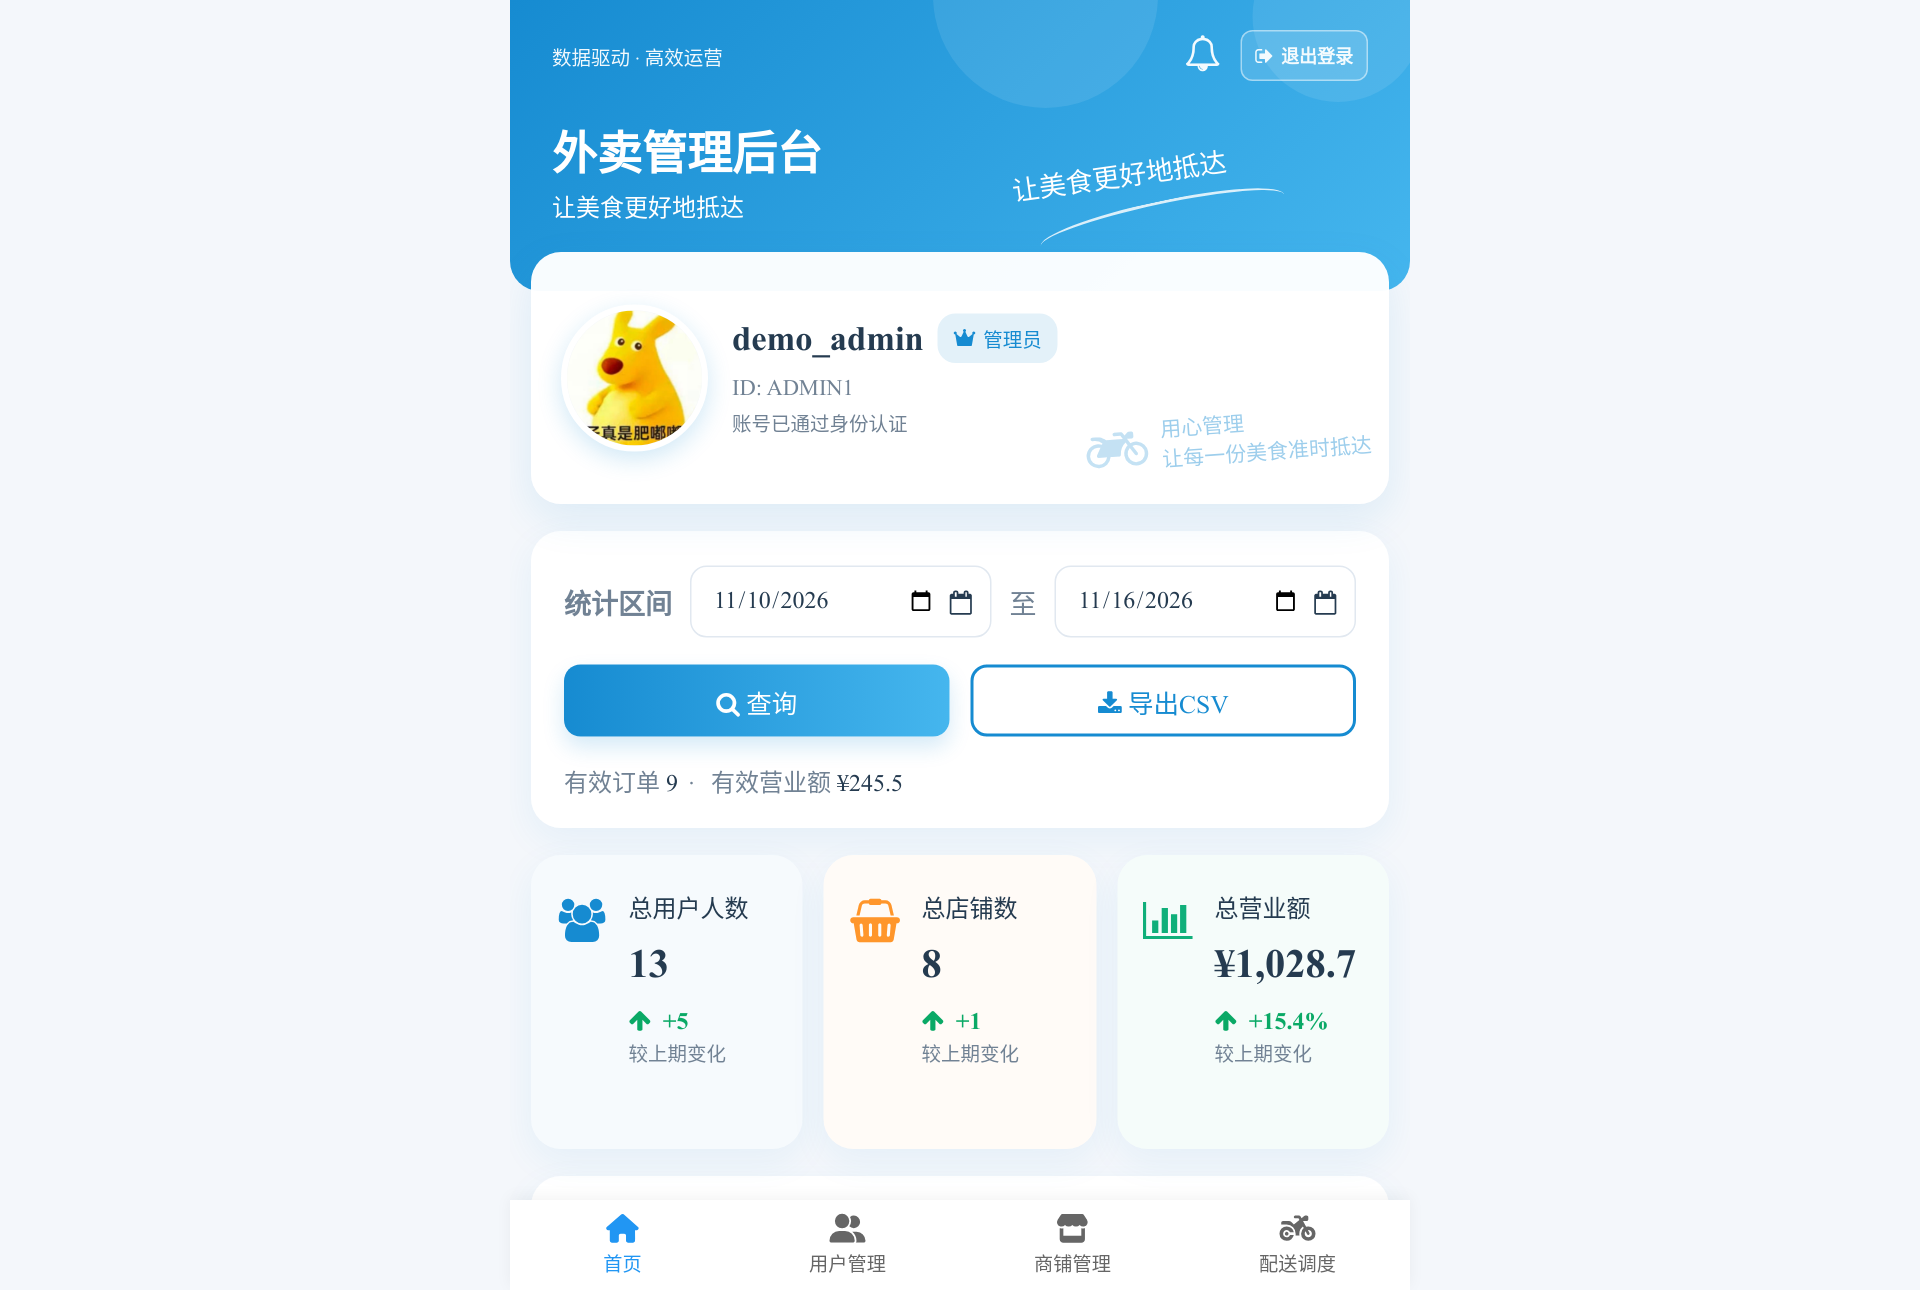
\includegraphics[width=0.96\linewidth,height=0.58\textheight,keepaspectratio]{figures/screenshots/ui-admin-home.png}}
  \caption{管理员端平台全局统计看板桌面运行界面（\code{/admin/home}，支持时间区间检索与 CSV 导出）}\label{fig:def-ui-admin-home}
\end{figure}

\begin{figure}[H]
  \centering
  \fbox{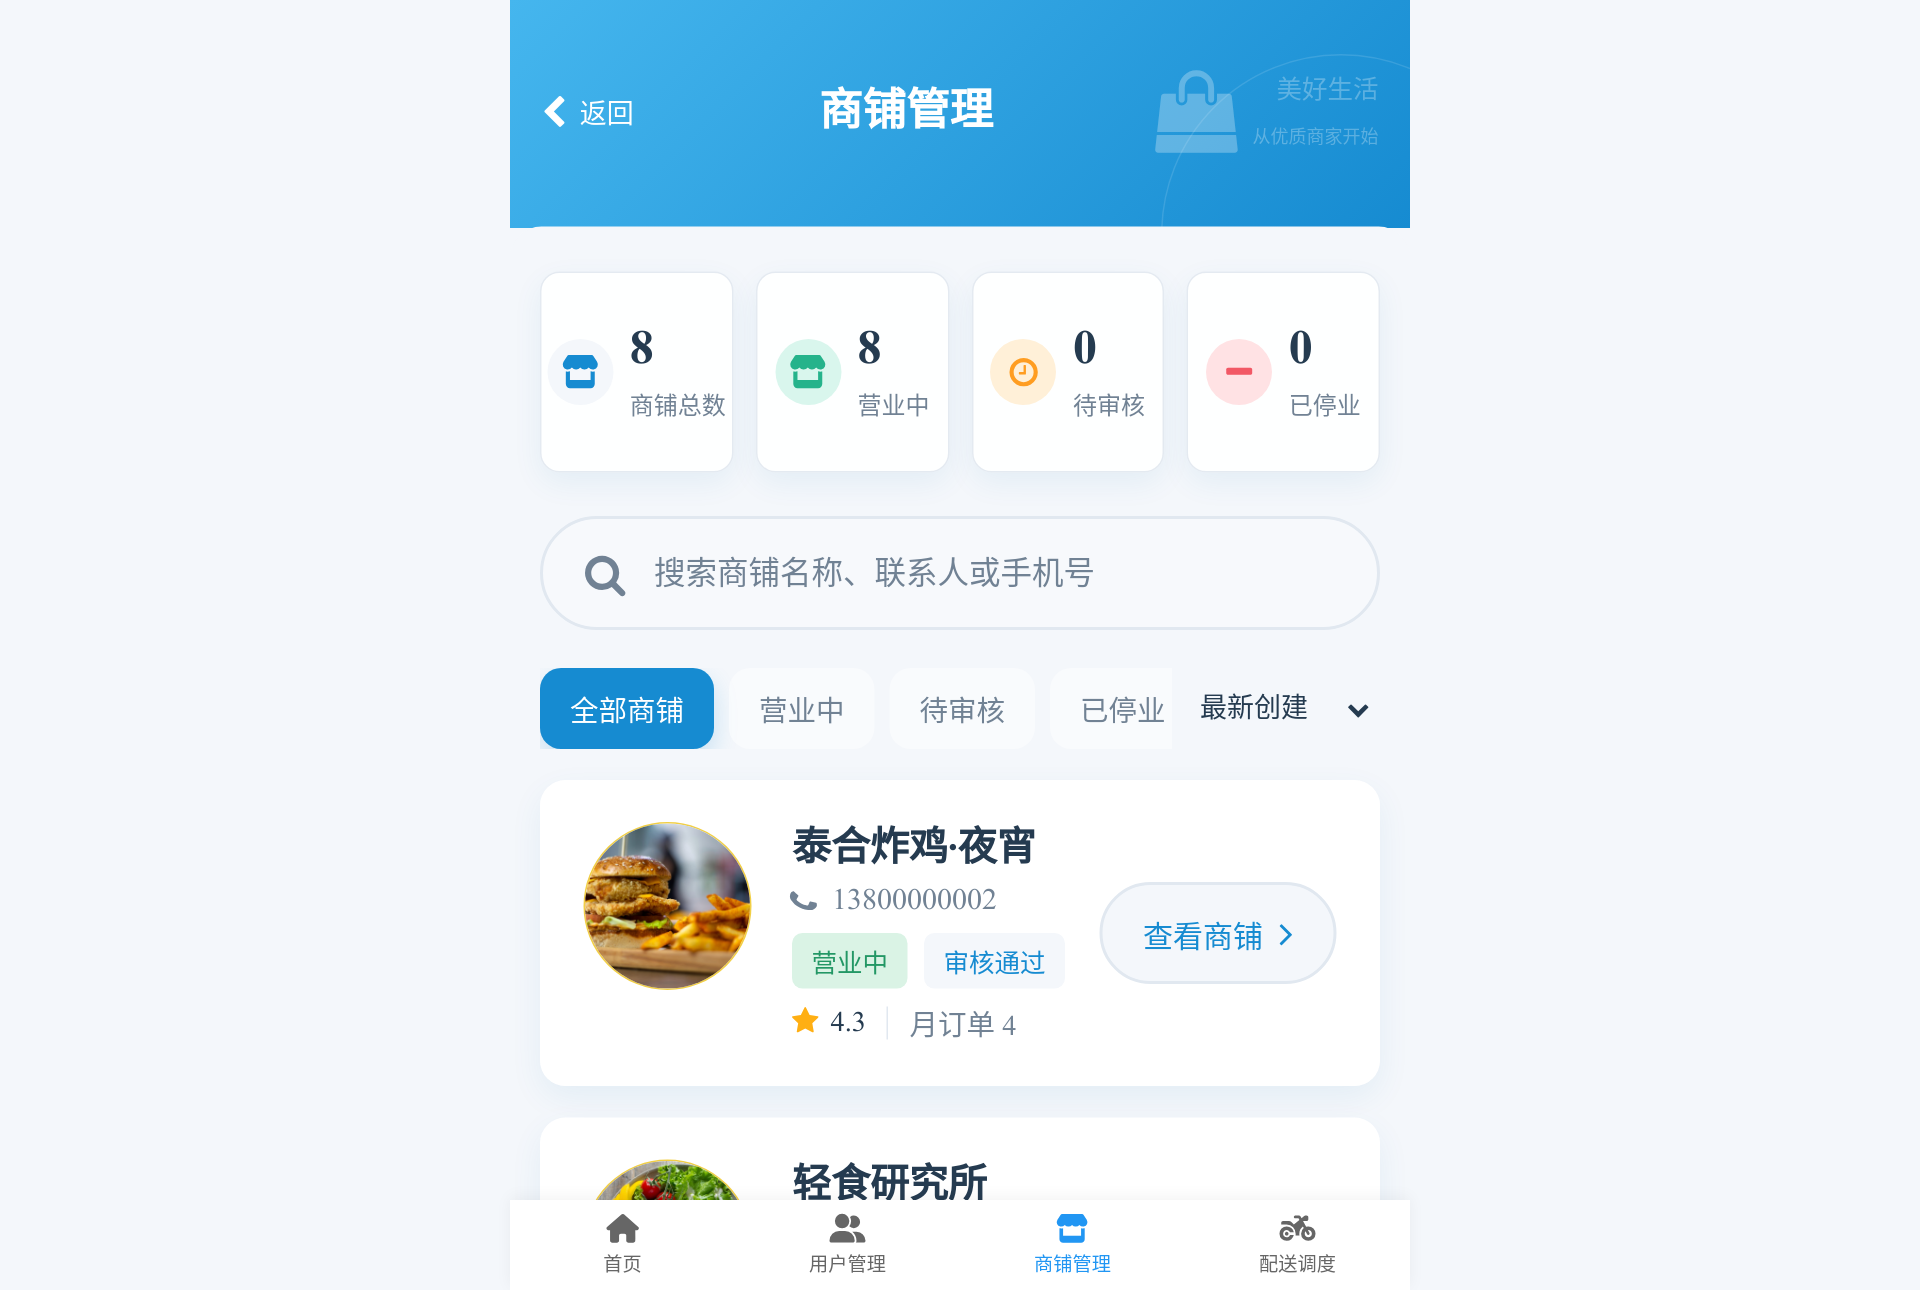
\includegraphics[width=0.96\linewidth,height=0.58\textheight,keepaspectratio]{figures/screenshots/ui-admin-businesses.png}}
  \caption{管理员端商铺入驻审批与营业状态治理界面（\code{/admin/business}）}\label{fig:def-ui-admin-biz}
\end{figure}

\uitwofig{figures/screenshots/ui-admin-users.png}{（a）平台用户账号启停与角色治理（\code{/admin/user}）}{figures/screenshots/ui-admin-riders.png}{（b）骑手入驻审核与配送异常仲裁（\code{/admin/riders}）}{管理员端账号治理与骑手/异常审核界面实景截图}{fig:def-ui-admin-users-riders}

\note{本次服务器未配置高德地图所需的 \code{AMAP_WEB_KEY}、\code{AMAP_JS_KEY} 与 \code{AMAP_SECURITY_CODE}。图~\ref{fig:def-ui-amap} 记录实际打开选址弹窗后出现的“地图服务尚未配置，仍可填写地址”提示，用于展示未配置时的降级状态；该图不作为地图瓦片、POI 搜索或真实定位成功的验证证据。}

\uifig[0.52\linewidth]{figures/screenshots/ui-amap-picker.png}{高德地图选址入口与服务未配置时的实际降级提示界面（\code{/addUserAddress}）}{fig:def-ui-amap}

  \chapter{过程管理}\label{chap:process}

开发期分为三个 Sprint。每轮从需求清单确定交付范围，评审时由组员在运行版本中按角色操作。265 次 Git 提交、34 个 Pull Request、飞书文档和 9 次腾讯会议记录保留了需求决议、返工和复测过程。

\section{Scrum 迭代与工程过程}

\subsection{在一次迭代里走完工程活动}

外送和自取的迭代包含沟通、策划、建模、构建和部署。团队先确认顾客需填写的信息与商家的检查项，再估算工时，在 SRS 和状态图中约定流程。页面与服务合入后，用运行版本走查订单。结算规则有分歧时，回到需求和模型核对。图~\ref{fig:proc-workflow} 展示了这些工作在 Scrum 中的顺序。

\begin{figure}[!htbp]
  \centering
  \resizebox{.92\linewidth}{!}{\begin{tikzpicture}[
  x=1pt,y=-1pt,
  stage/.style={draw=#1!70,fill=#1!7,rounded corners=2pt,line width=.48pt,
    minimum height=28pt,minimum width=93pt,inner sep=3pt,align=center,
    font=\fontsize{10bp}{12bp}\selectfont},
  direction/.style={-{Stealth[length=3.6pt,width=3.1pt]},draw=procink,line width=.6pt},
  annotation/.style={font=\fontsize{8.4bp}{10bp}\selectfont,fill=white,inner sep=1.6pt}
]
  \definecolor{procink}{HTML}{394D59}
  \definecolor{procslate}{HTML}{476C82}
  \definecolor{procsage}{HTML}{397A70}
  \definecolor{procsand}{HTML}{957048}
  \node[stage=procslate] (backlog) at (51,16) {\textbf{Product Backlog}\\REQM 需求基线};
  \node[stage=procslate] (plan) at (161,16) {\textbf{Sprint 规划}\\PP 任务估算};
  \node[stage=procslate] (develop) at (271,16) {\textbf{特性分支开发}\\CM / PMC 日同步};
  \node[stage=procsand] (gate) at (381,16) {\textbf{TDD 与 PR 门禁}};
  \node[stage=procsage] (review) at (51,83) {\textbf{Sprint 评审}\\VAL 增量验收};
  \node[stage=procsage] (retro) at (161,83) {\textbf{Sprint 回顾}\\OPF 过程改进};
  \node[stage=procsage] (release) at (271,83) {\textbf{基线交付}\\VER 归档与部署};
  \draw[direction] (backlog.east) -- (plan.west);
  \draw[direction] (plan.east) -- (develop.west);
  \draw[direction] (develop.east) -- (gate.west);
  \draw[direction] (review.east) -- (retro.west);
  \draw[direction] (retro.east) -- (release.west);
  \draw[direction,rounded corners=3pt] (gate.south) -- (381,115)
    -- node[annotation,pos=.48,above]{575 项测试通过} (51,115) -- (review.south);
  \draw[direction,dashed,draw=procsage] (retro.north)
    -- node[annotation,right,text=procsage]{改进项反哺下轮} (plan.south);
\end{tikzpicture}
}
  \caption{CMM3 过程域与 Scrum 敏捷迭代融合工作流图}\label{fig:proc-workflow}
\end{figure}

一次自取验收中，两端分别通过检查后，团队在评审时走完同一笔订单，验证省略收货地址能否提交。在迭代回顾中，组员再追查为什么两端到联调时才统一规则，并把需要提前确认的条件带入下一轮规划。

\subsection{CMM3 过程域在本项目中的实践映射}

项目沿用 CMM 已定义级强调的过程记录，并按迭代需求裁剪。各端用同一份 SRS 核对规则，每轮更新发生变化的任务、接口和测试，方便成员交接。需求管理、项目策划、验证和确认的对应材料见附录表~\ref{tab:cmm3-mapping}。

调整自取规则时，赵紫怡确认收货地址可省略，并核对订单状态说明。前端结算和后端计价按这一约定修改，再复测外送和自取。版本管理、评审与质量检查贯穿迭代。任务单保存变更内容，PR 记录合入情况，测试核对规则是否落实。

\subsection{需求、迭代与代码怎样交接}

赵紫怡担任 Product Owner，确定需求范围和优先级。李承文担任 Scrum Master，组织迭代，协调阻塞事项、风险和合并检查。四位成员共同交付每轮增量，分别在飞书和 GitHub 记录需求进度与代码评审。图~\ref{fig:proc-repo} 为课程提供的 Gitee 基础仓库，图~\ref{fig:proc-feishu} 为小组的飞书共享空间。

\begin{figure}[!htbp]
  \centering
  \begin{minipage}[t]{.485\linewidth}
    \centering\vspace{0pt}
    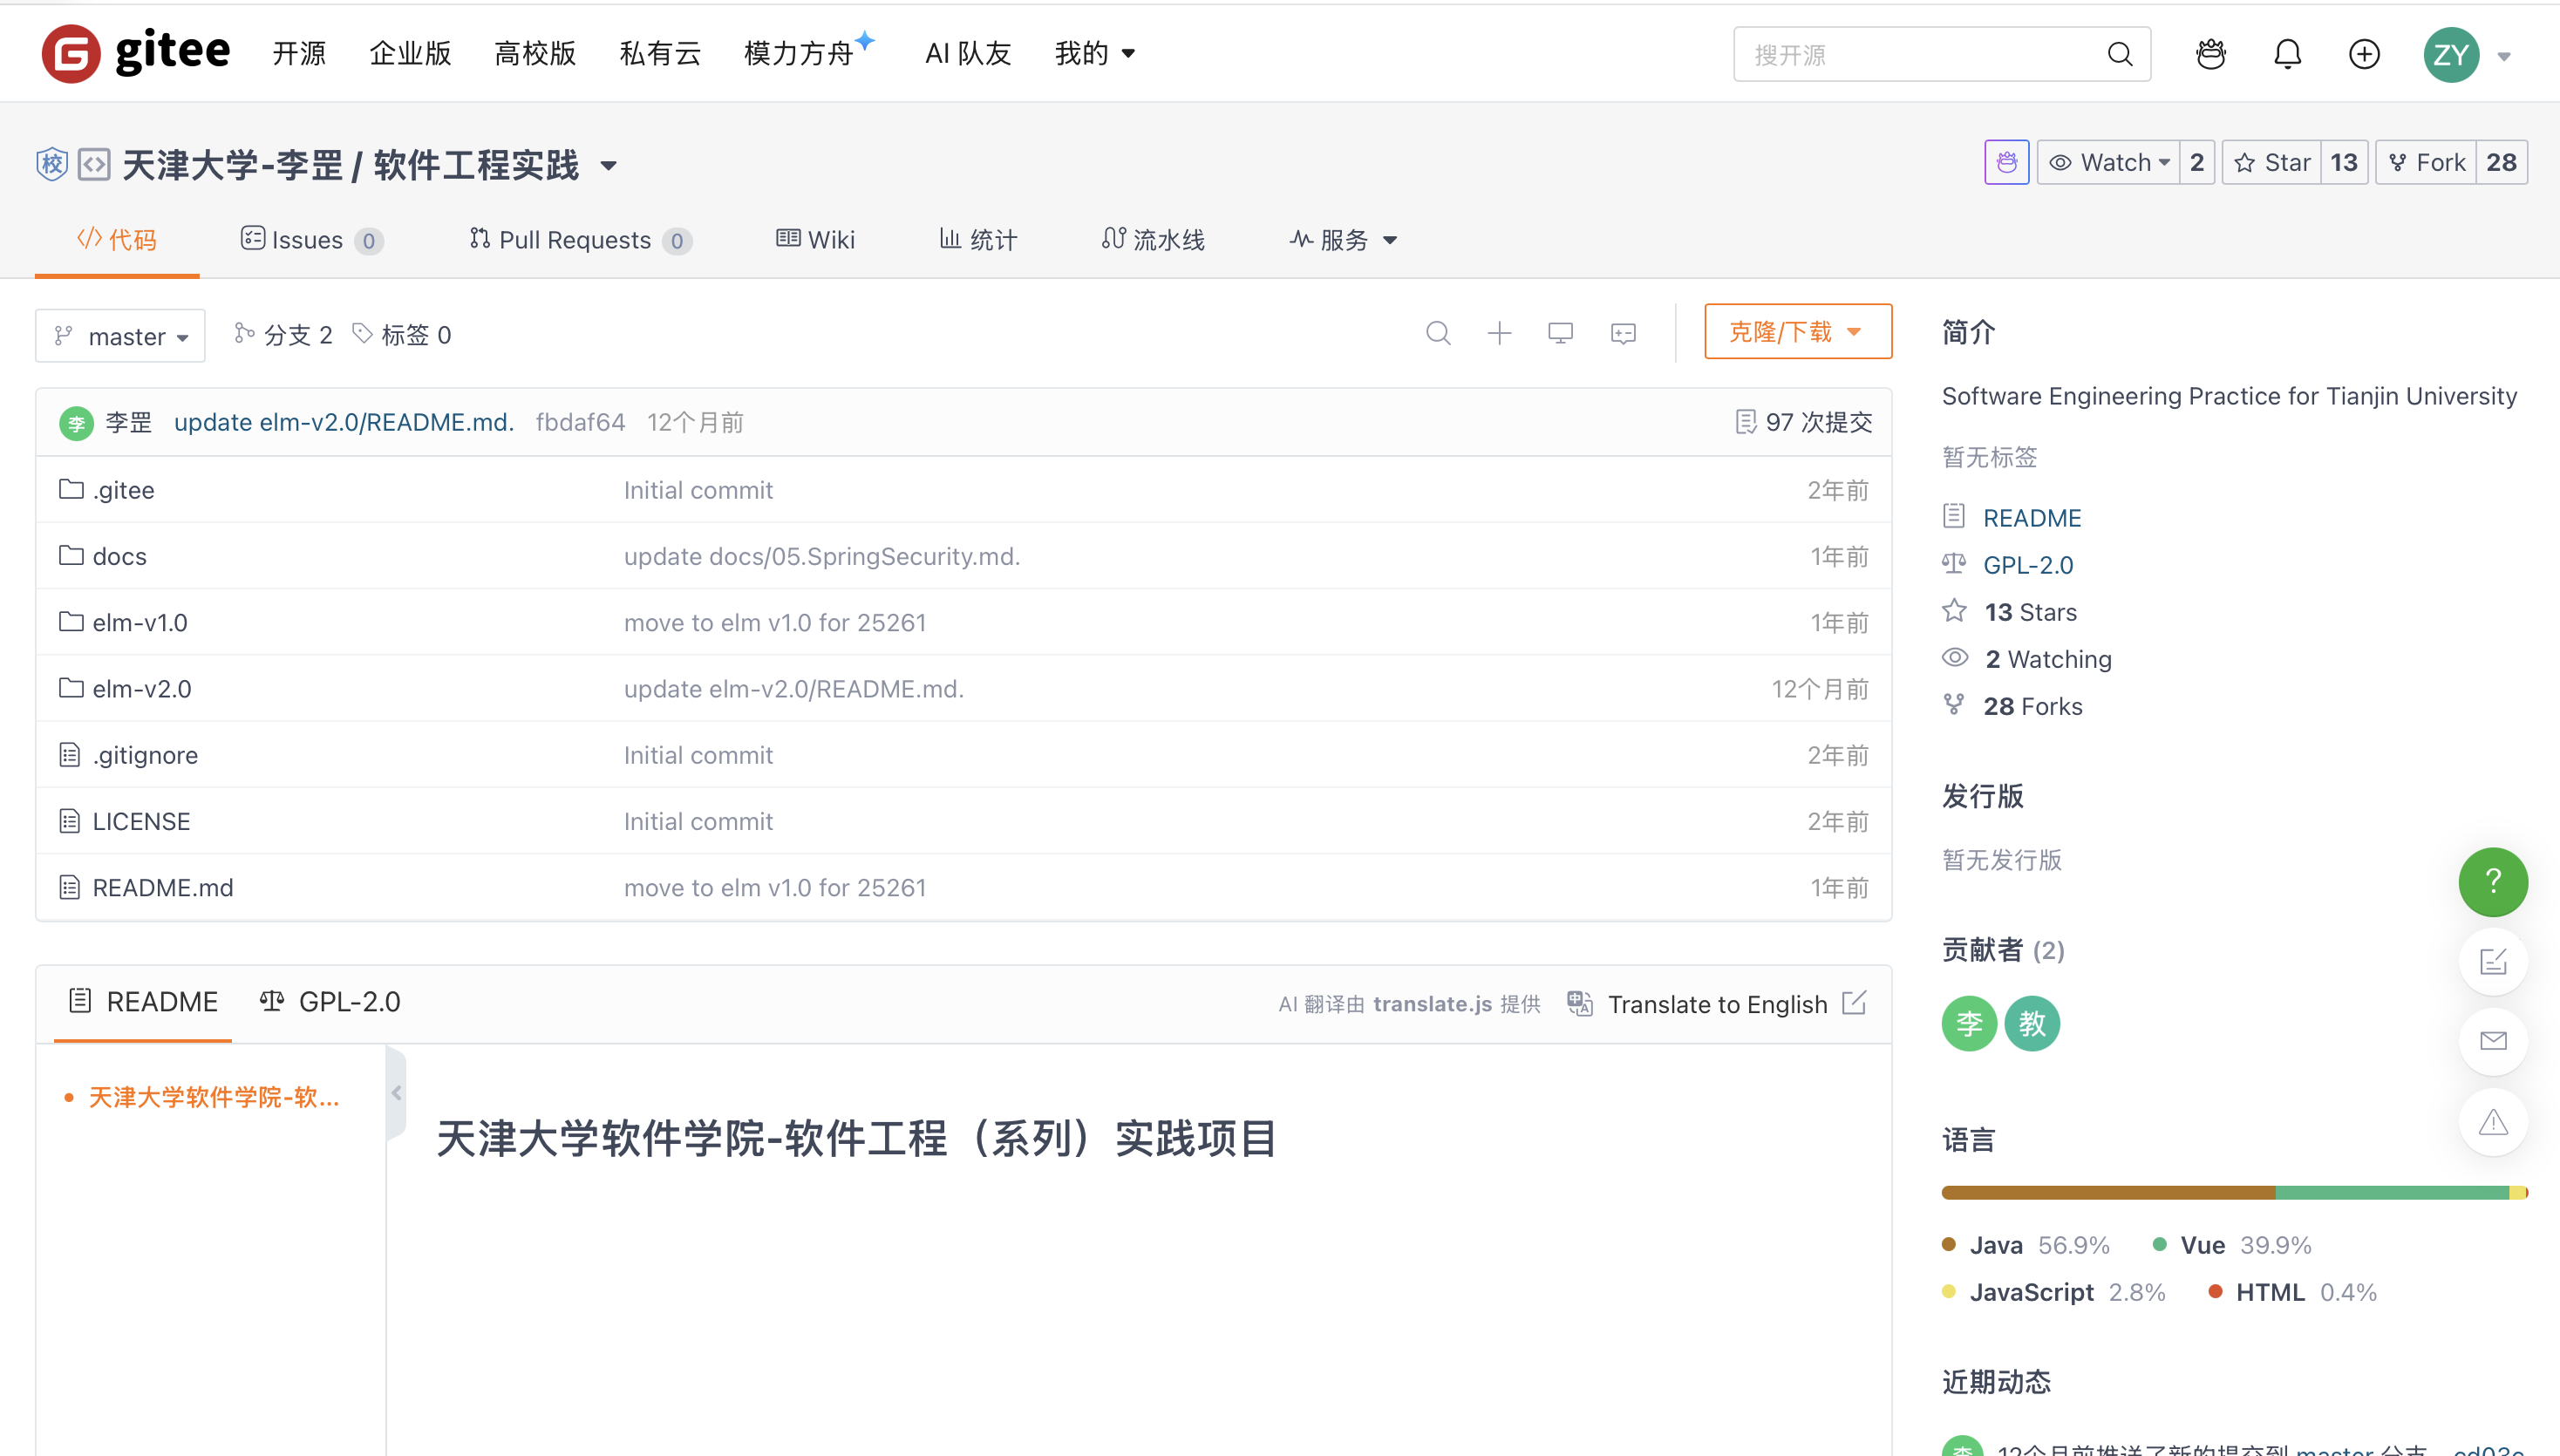
\includegraphics[width=\linewidth,height=.23\textheight,keepaspectratio]{figures/report/process/course-repository.png}
    \captionof{figure}{Gitee 课程仓库分支、目录与提交记录}\label{fig:proc-repo}
  \end{minipage}\hfill
  \begin{minipage}[t]{.485\linewidth}
    \centering\vspace{0pt}
    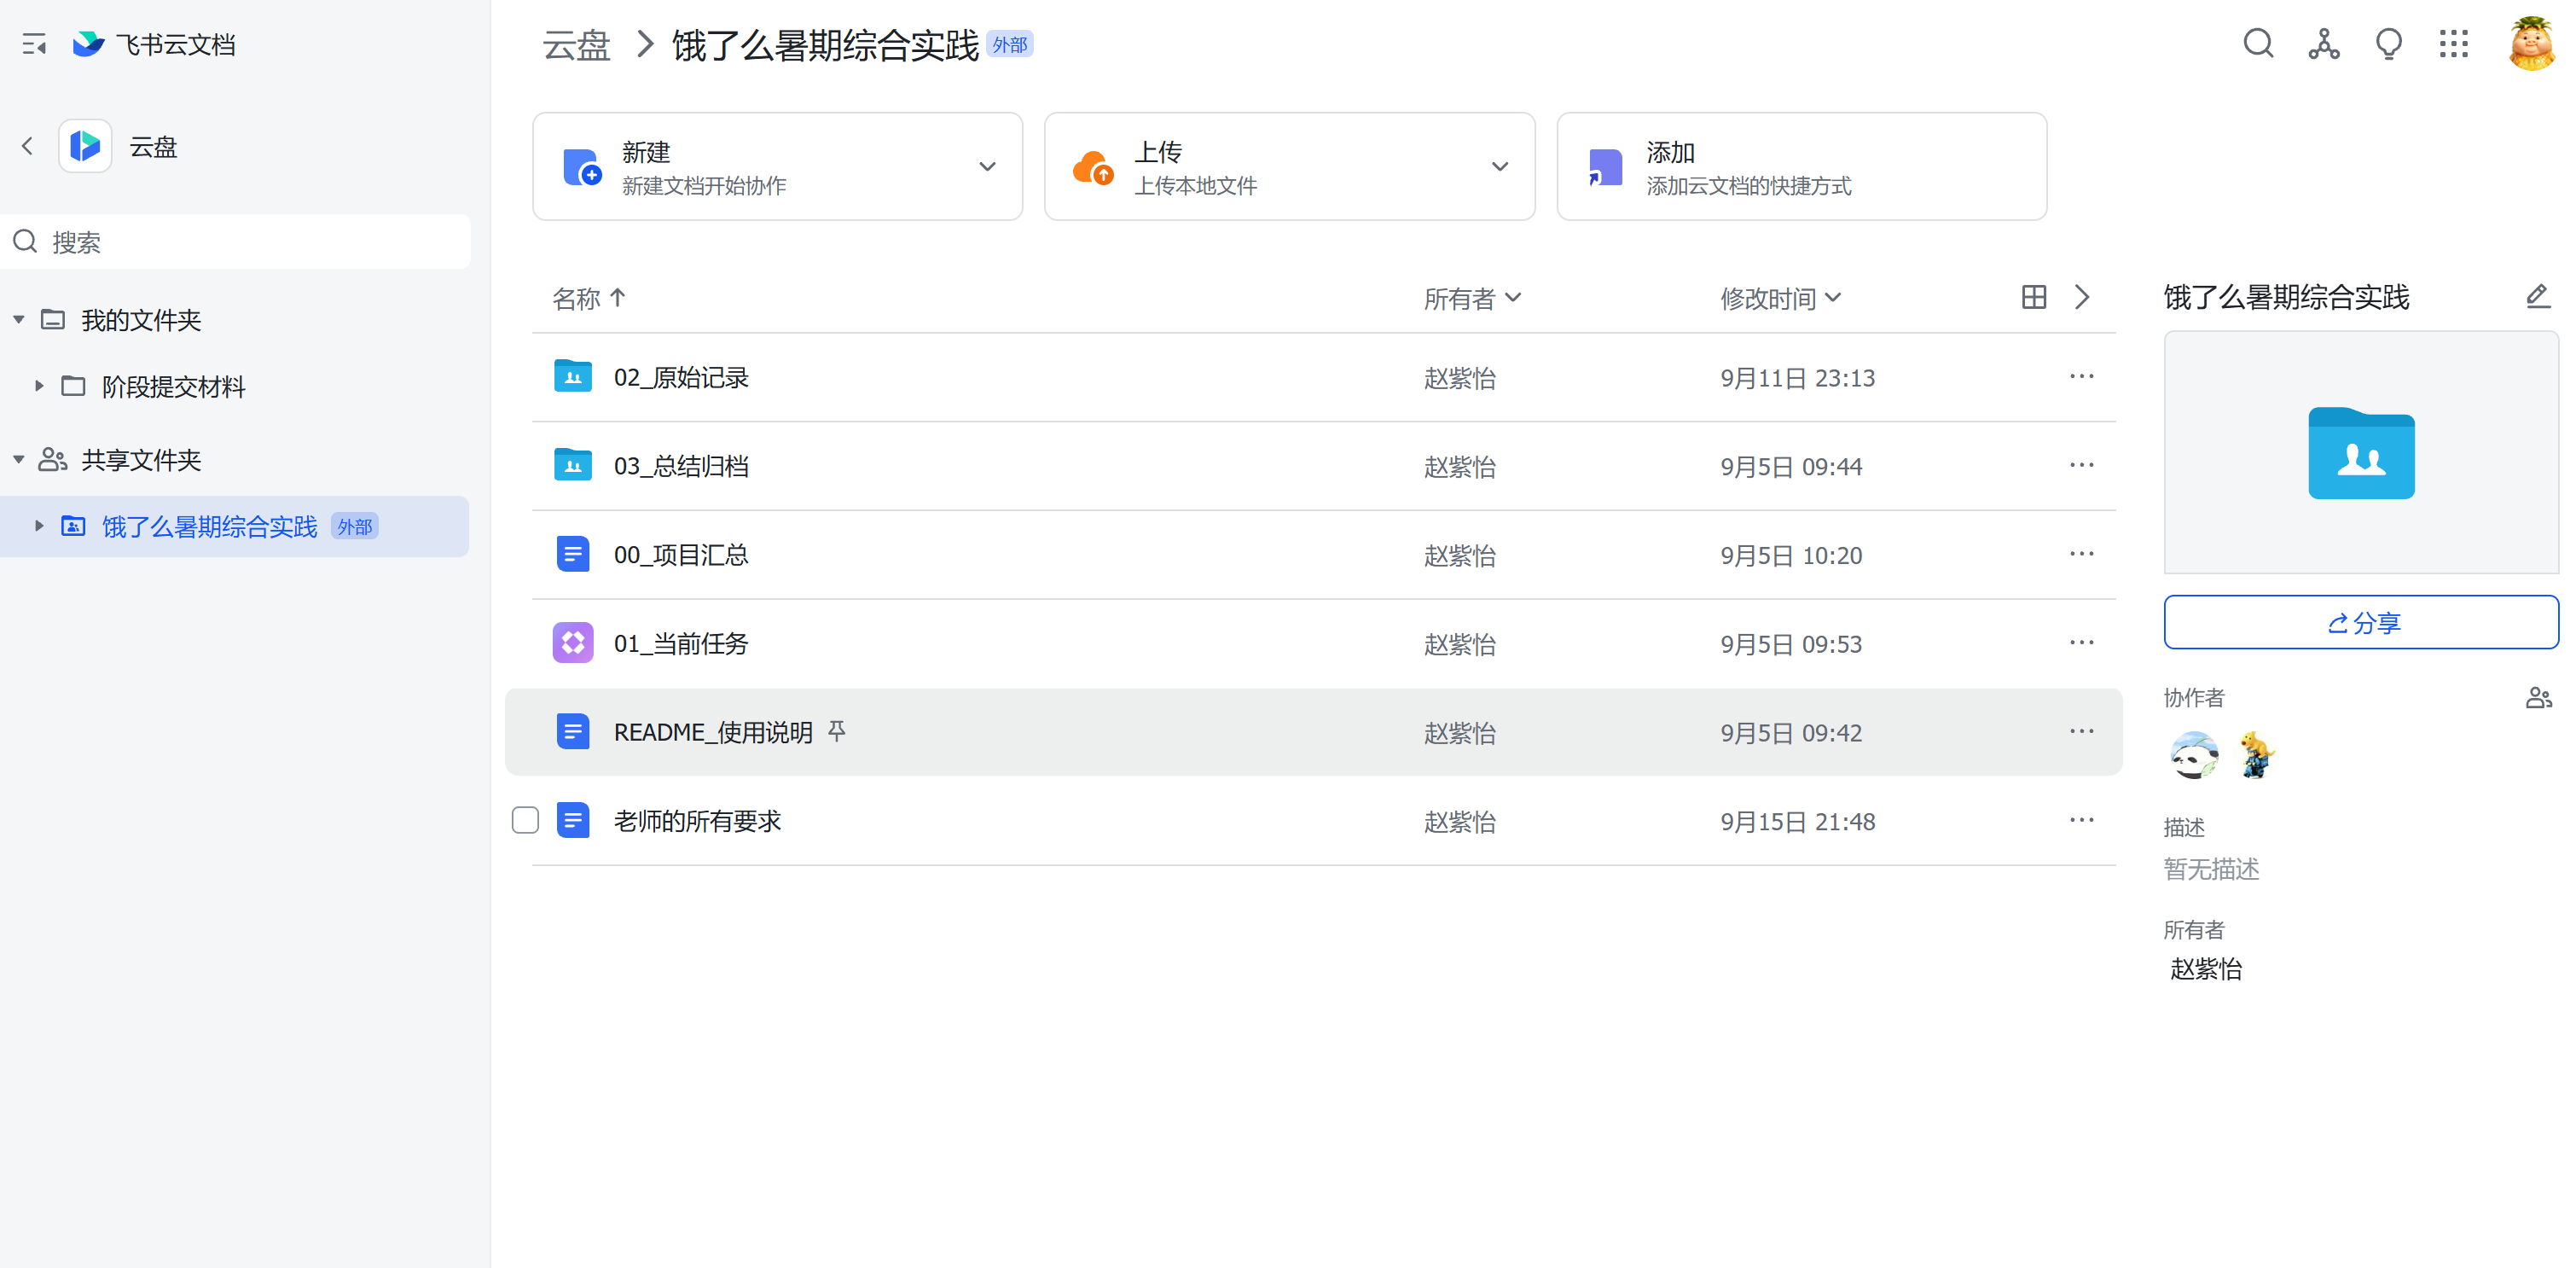
\includegraphics[width=\linewidth,height=.23\textheight,keepaspectratio]{figures/report/process/feishu-workspace.png}
    \captionof{figure}{飞书共享协作空间与任务状态/会议纪要归档视图}\label{fig:proc-feishu}
  \end{minipage}
\end{figure}

\subsection{需求记录与合并检查}

自取规则变更可以从飞书任务追到具体版本。需求单写明负责人和自取结算条件，分支保留计价与页面改动。测试人员分别核对自取与外送，保存下单记录和接口结果，便于追查上次调整的原因。

合并前用 \code{scripts/check-repository.mjs} 检查仓库能否独立检出和部署。检查项包括 README、需求规格、部署说明、相对链接，以及 Compose 引用的挂载文件。部署目标从配置读取，脚本检查个人绝对路径和硬编码部署地址。接口、事务和页面行为由各自的测试覆盖，仓库检查验证交付材料和运行配置能否随项目迁移。

\section{立项组会与阶段会议记录}

\subsection{立项组会快照}

2026 年 9 月 1 日 20:00--21:30，四位成员召开第一次全体会议。李承文主持，赵紫怡在飞书同步记录，范文丽和仲禹潼共同讨论前端页面、角色边界及验收办法。会上确定了项目名称、角色分工、Git 工作流、数据库演进规则和第一轮迭代目标。

\subsection{核心决议}

\begin{reportpoints}
\item 顾客下单和商家履约作为基础，加入骑手配送工作台。地图负责选址与导航，资产模块覆盖模拟钱包、会员、优惠券及积分，多模态 AI 辅助顾客点餐。
\item 后端使用 \code{elm_bk}（Spring Boot 3.4.6、Java 17），前端使用 \code{elmclient}（Vue 3）。成员在特性分支上开发，发起 PR 后由 Scrum Master 复核并合入 \code{main}。
\item 服务端负责核对金额、库存和访问权限。菜品名称和成交单价在下单时写入 \mbox{\code{orderdetailet}}，历史明细读取这份成交记录。
\item 主开发从 9 月 1 日到 9 月 19 日，分为 9 月 1--7 日、8--12 日和 13--19 日三轮。9 月下旬继续整理跨组交叉验收与交付文档。
\end{reportpoints}

\subsection{即时任务分配（RACI 责任矩阵）}

立项时，团队用表~\ref{tab:raci} 明确各项工作的执行（R）、批准（A）、咨询（C）和知会（I）角色。跨成员任务出现分歧时，可按责任矩阵找到确认人。

\begin{table}[H]
  \centering
  \caption{项目核心工程活动 RACI 责任矩阵}\label{tab:raci}
  \reporttablesize
  \begin{tabular}{@{}L{.405\linewidth}C{.135\linewidth}C{.135\linewidth}C{.135\linewidth}C{.135\linewidth}@{}}
\toprule
\textbf{工程活动 / 交付物} & \textbf{范文丽} & \textbf{李承文} & \textbf{赵紫怡} & \textbf{仲禹潼} \\
\midrule
SRS 编写与 UML 建模 & C & C & R/A & C \\
前端四端页面、主题与数据看板 & R/A & C & I & C \\
后端认证、订单、资产与配送接口 & C & R/A & C & I \\
MySQL 表结构与增量迁移设计 & I & C & R/A & I \\
AI 智能点餐与多模态适配 & R & C & R/A & C \\
高德地图选址、距离与导航 & C & C & I & R/A \\
自动化测试、WPS 缺陷台账与\mbox{交叉验收} & C & C & C & R/A \\
Docker 容器编排与 PR 主干合并 & I & R/A & I & C \\
\bottomrule
  \end{tabular}
\end{table}

AI 点餐由赵紫怡和范文丽联调。赵紫怡维护需求和模型接口，范文丽负责输入与展示，李承文核对接口及主干合并，仲禹潼按顾客的操作进行验收。模型不可用时，对照后端返回与页面提示即可定位问题。

菜名快照由赵紫怡确定字段和迁移脚本，李承文核对订单写入和查询，前端与测试再打开历史订单。验收条件是商家改名后，顾客仍能看到成交时的菜名。发现差异时按写入、查询、显示的顺序排查。

\subsection{阶段线上组会纪要汇总}

开发与验收期间，团队通过站会同步当天工作，另在腾讯会议上召开 9 次专题会，确认跨模块问题。会议列表见图~\ref{fig:proc-meetings}，决议和行动记录见附录表~\ref{tab:meeting-log}。

\begin{figure}[H]
  \centering
  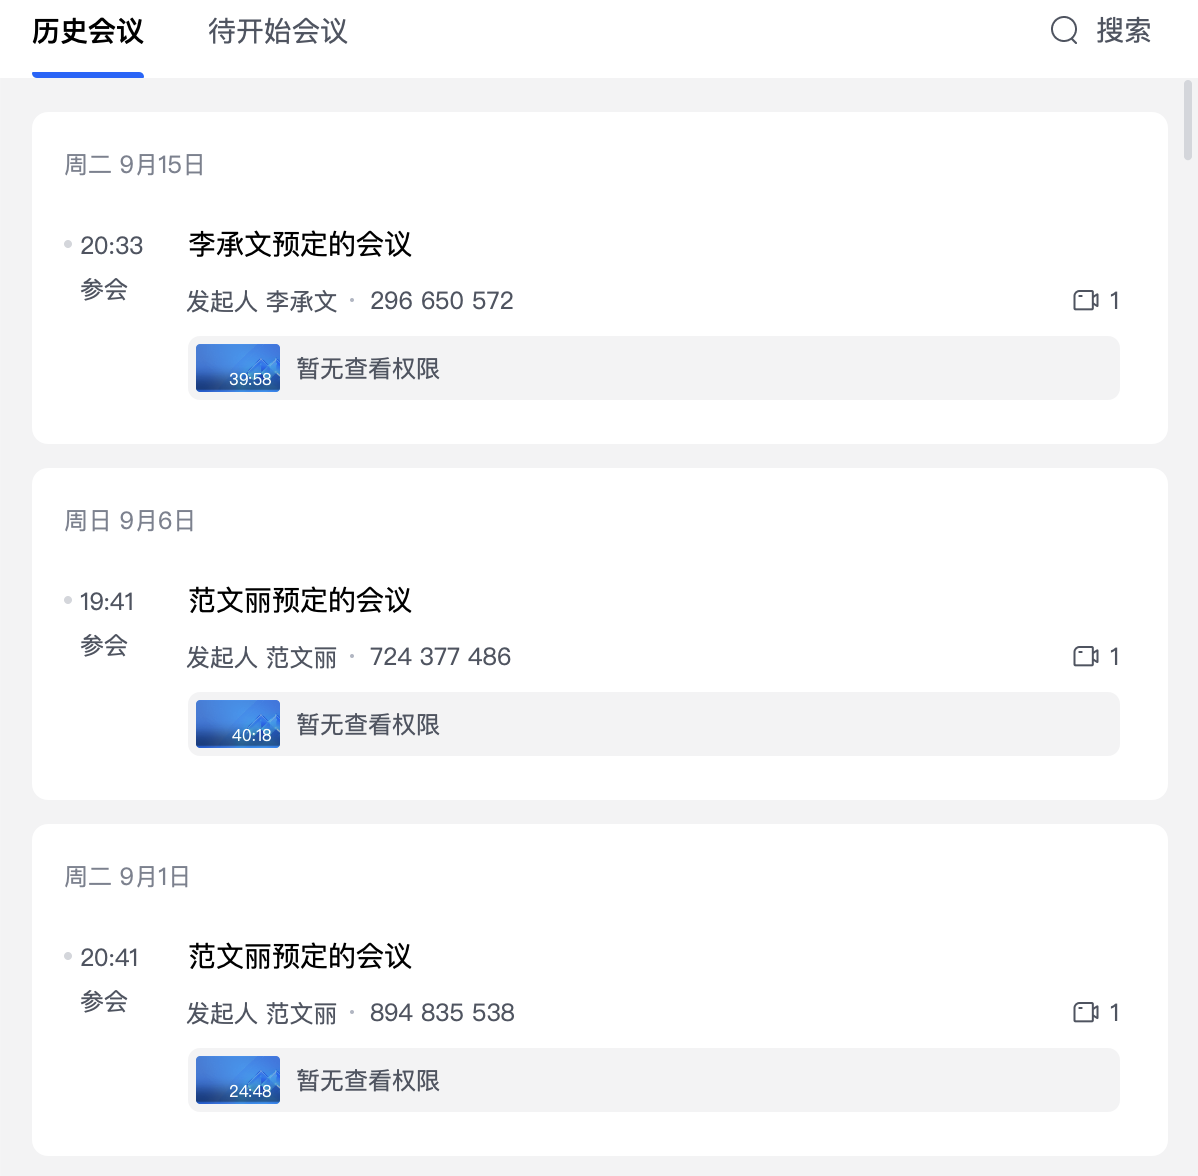
\includegraphics[width=.88\linewidth,height=.50\textheight,keepaspectratio]{figures/report/process/meeting-history.png}
  \caption{团队腾讯会议阶段例会线上历史记录截图}\label{fig:proc-meetings}
\end{figure}

9 月 5 日的接口会统一 JWT 身份、商家和商品字段及订单状态编码。9 月 6 日中期检查处理未登录跳转、字段遗漏和自取规则。第二轮转入多分支合并和公共接口开发。9 月 10 日确定新增接口使用 \code{/api/v1/}，9 月 12 日首次集中联调时，把页面操作、接口响应和后续改动记入同一份 WPS 缺陷台账。9 月 15 日确定封板版本，随后两次会议核对跨组验收发现、演示数据与归档材料。

会后按决议检查合入结果。9 月 10 日确定接口路径后，复查页面实际调用。9 月 15 日封板后，核对 AI 分支、公共外壳及导航修复的合入情况，并复跑 \mbox{原有操作路径}。

\Needspace{.61\textheight}
\section{Sprint 迭代管理}

第一轮交付店铺浏览和下单，第二轮接入商家处理、骑手配送和资产功能，第三轮补充管理端和外部服务。各轮复测已有流程，包括旧订单菜名和页面返回。四类账号的界面见图~\ref{fig:proc-four-roles}，分工和站会记录见附录~\ref{app:process}。

\begin{figure}[H]
  \centering
  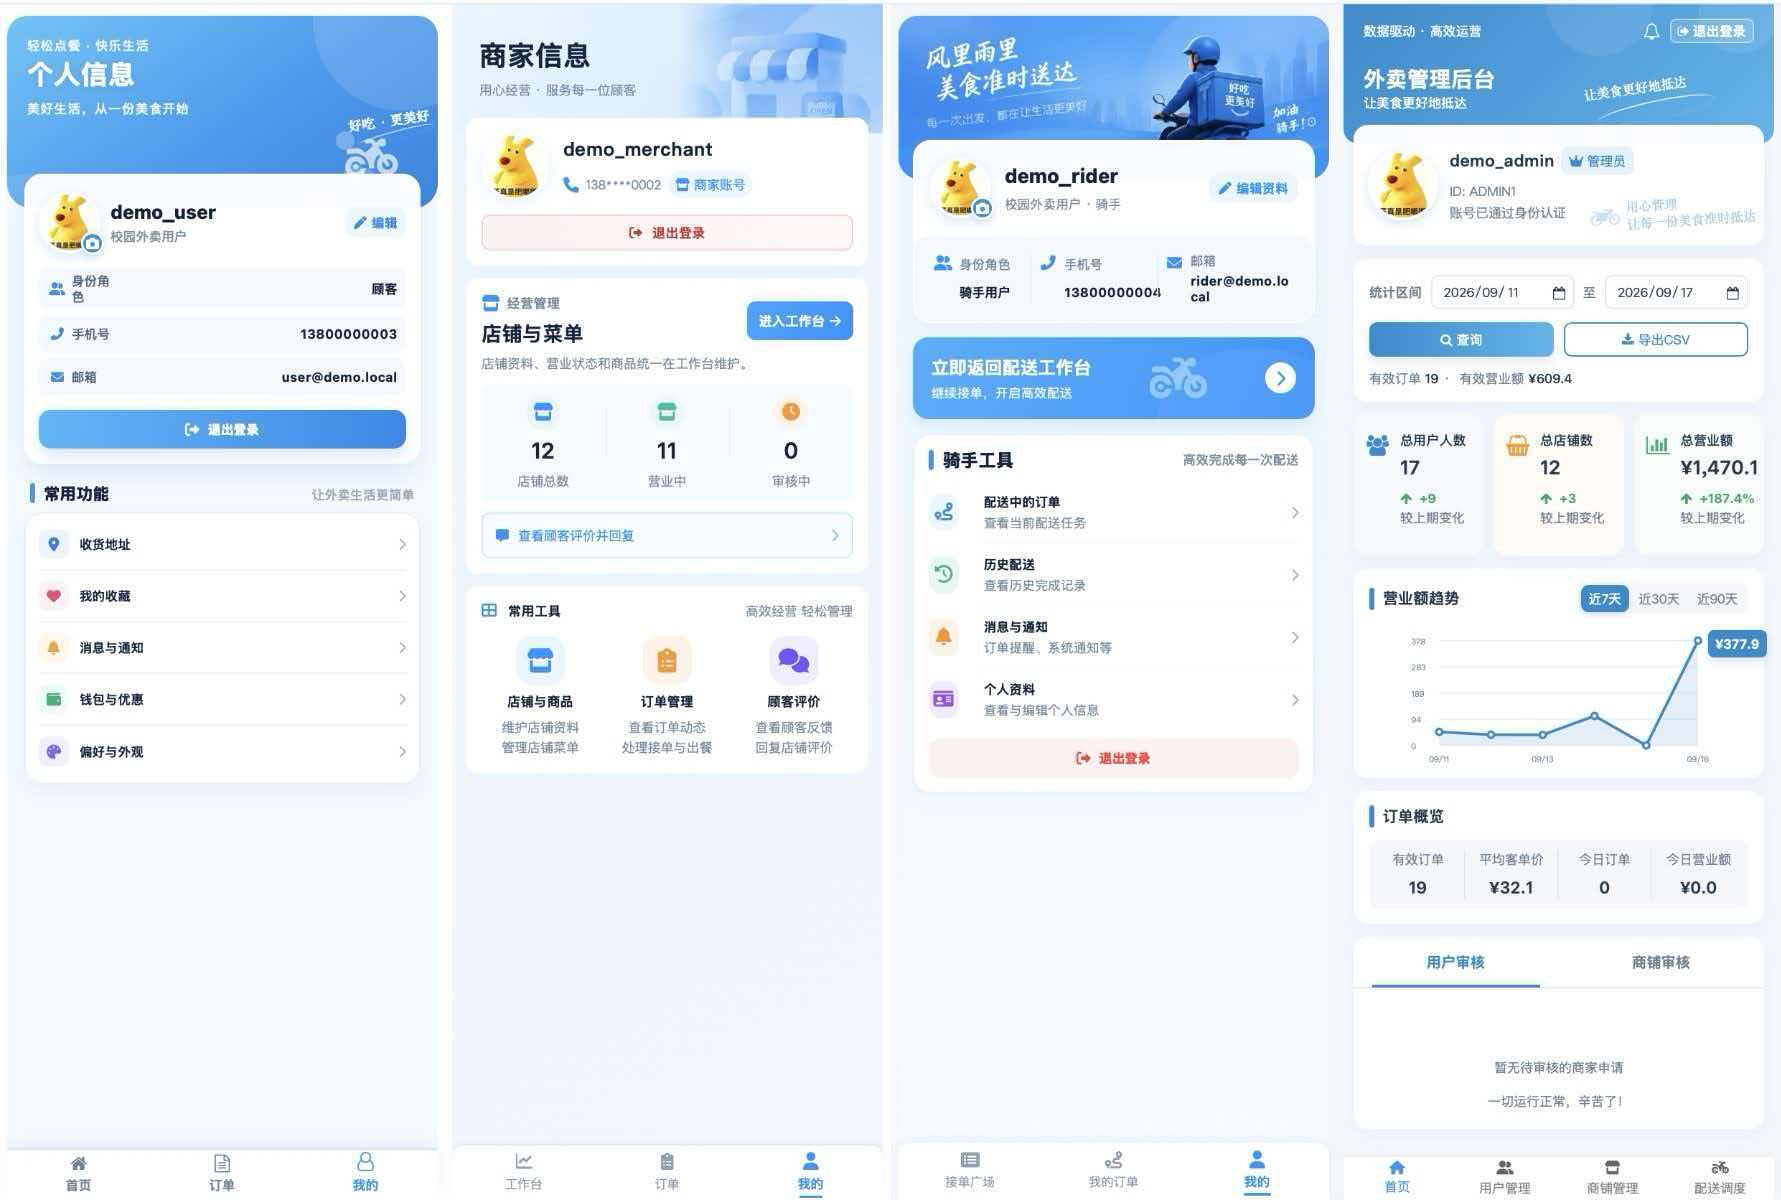
\includegraphics[width=.95\linewidth,height=.46\textheight,keepaspectratio]{figures/report/process/four-roles.jpg}
  \caption{四端核心账号（顾客、商家、骑手、管理员）工作台并行联动效果全景}\label{fig:proc-four-roles}
\end{figure}

顾客从底栏查看订单结果和履约进度。商家在工作台处理本店订单，骑手通过接单广场和配送工作台查看任务，管理员在首页查看平台数据并进入审核与调度。最终联调沿\textbf{同一订单编号}检查四端的操作权限和状态变化，完成履约验收。

\subsection{Sprint 1 需求建模、基础认证与顾客下单核心闭环（9 月 1 日--9 月 7 日）}

\subsubsection{迭代目标与任务拆解}
第一轮计划交付 42 个故事点，投入 80 小时，任务见表~\ref{tab:sprint1-tasks}。团队先确定 SRS 和数据库基线，再实现顾客侧 P0 最小可用版本。首轮评审覆盖游客浏览店铺和菜单，以及登录后的加购、下单、查单和取消。

\subsubsection{每日站会与工作日志（问题与解决过程）}
9 月 3 日和 9 月 7 日是本轮两个集中提交点，分别有 60 次和 35 次提交，主要涉及建模文档和基础认证、编排。附录表~\ref{tab:sprint1-daily} 记录了本轮各日的进展。前半周先把需求写清楚，后半周才有可以连续操作的顾客流程。

团队以 \code{4fcbf00} 初始化课程仓库，并用四端角色组织 SRS 用例。9 月 3 日提交 SRS 初版 \code{6e39d85} 后，大家发现 draw.io 批量导出时有连线错位。统一编号和导出校验后，重新生成了 17 张建模图。接下来清理了构建产物与缓存，统一仓库图片目录，文档可以和代码一道在 PR 中审阅。9 月 6 日的 SRS 2.0 合并保留了已经确认的用例与状态约定，后端骨架和持久化同时继续开发。

首轮联调发现两类交易问题。菜品改名或改价后，历史订单可能读取更新后的商品信息。团队用 \code{003_order_name_snapshot.sql} 补充名称快照，查询改为读取订单明细。回归用例先改商品，再打开原订单，检查成交时的菜名与价格。自取结算起初沿用了外送地址和起送价校验。团队在 \code{OrderPricingService} 中按履约方式计价，前端依据所选方式调整结算项。

9 月 7 日完成认证测试、商铺目录联调和 Docker 基础编排后，评审可以从头操作一次。成员先以游客身份浏览，再登录顾客账号加购，提交订单后检查列表和取消。与规格不一致的步骤会反馈给维护页面、服务或数据库的成员，连同用例编号记录在任务清单。这个顺序也为下一轮商家与骑手接手同一笔订单准备了数据。

首轮按公共目录、登录态、订单提交和回退拆分任务。游客可浏览公共店铺，打开购物车时需要登录。取消订单需校验归属并恢复库存和资产，顾客端按钮随服务端订单状态变化。各项通过后再连续操作一遍，检查登录跳转、页面读写\mbox{和数据状态能否衔接}。

\subsubsection{迭代燃尽图、评审与回顾}
产品负责人和组员共同评审注册、登录、游客浏览、加购、下单与取消，结果见表~\ref{tab:sprint1-review}。快照和自取修复使剩余工时在 9 月 5 日偏离理想线，\mbox{9 月 7 日归零（图~\ref{fig:burndown-s1}）}。

折线在 9 月 4 日至 5 日只下降 3 小时，剩余工作从 45 小时减到 42 小时，是首轮收敛最慢的一段。收尾评审沿顾客流程检查补丁合入后的历史菜名、自取提交和取消时的数据恢复。

\begin{figure}[!htbp]
  \centering
  \resizebox{.86\linewidth}{!}{%
\begin{tikzpicture}[x=1.52cm,y=0.059cm]
    \definecolor{proctrend}{HTML}{25465D}
    \definecolor{procaxes}{HTML}{3F505E}
    \definecolor{procgrid}{HTML}{DFE5E9}
    \foreach \y in {0,20,40,60,80} {
      \draw[procgrid,line width=.4pt] (0,\y) -- (6.72,\y);
      \node[left,font=\scriptsize,text=procaxes] at (0,\y) {\y};
    }
    \draw[procaxes,line width=.52pt] (0,90) -- (0,0) -- (6.72,0);
    \foreach \d/\lbl in {0/9.1,1/9.2,2/9.3,3/9.4,4/9.5,5/9.6,6/9.7} {
      \draw[procaxes,line width=.45pt] (\d,0) -- ++(0,-2.5pt);
      \node[below=3pt,font=\scriptsize,text=procaxes] at (\d,0) {\lbl};
    }
    \node[anchor=south west,inner sep=1pt,font=\scriptsize,text=procaxes] at (0,90) {剩余工时 (h)};
    \node[anchor=north east,inner sep=0pt,font=\scriptsize,text=procaxes] at (6.72,-15pt) {日期 (9月)};

    \draw[procaxes,dash pattern=on 3pt off 2.6pt,line width=.62pt] (0,80) -- (6,0);
    \draw[proctrend,line width=.92pt] plot[mark=*,mark size=1.6pt,mark options={solid,fill=white,line width=.72pt}]
      coordinates { (0,80) (1,70) (2,54) (3,45) (4,42) (5,22) (6,0) };

    \draw[procaxes,dash pattern=on 3pt off 2.6pt,line width=.62pt]
      (4.05,78) -- ++(16pt,0) node[right=3pt,font=\scriptsize,text=procaxes] {理想基准线};
    \draw[proctrend,line width=.92pt] (4.05,69)
      -- ++(16pt,0) node[right=3pt,font=\scriptsize,text=procaxes] {实际剩余工时};
    \draw[proctrend,fill=white,line width=.72pt] (4.235,69) circle[radius=1.6pt];
  \end{tikzpicture}
}
  \caption{Sprint 1 迭代工时燃尽图（9 月 1 日--9 月 7 日，总工时 80 h）}\label{fig:burndown-s1}
\end{figure}

\begin{longtable}{L{.18\linewidth}L{.44\linewidth}L{.29\linewidth}}
\caption{Sprint 1 迭代评审验收与回顾总结表}\label{tab:sprint1-review}\\
\toprule
\textbf{评估维度} & \textbf{核心结论与验收事实} & \textbf{沉淀行动项（Try）} \\
\midrule
增量评审（Review） & \code{US001--US007} 中顾客核心点餐链路全部跑通。完成认证与商品目录 2 轮 TDD 提交。Docker 基础服务可正常启动。 & 在 Sprint 2 全面推行“RED-GREEN-REFACTOR”三步\mbox{提交模式。} \\
过程回顾（Keep/Prob） & 保留飞书任务与 PR 审查节奏。初版接口未对齐自取规则，结算联调中\mbox{补做了调整。} & 新增“业务枚举与状态编码变更必须在组会\mbox{同步后再编码”规范。} \\
\bottomrule
\end{longtable}

\subsection[Sprint 2 商家工作台、骑手配送闭环\texorpdfstring{\protect\newline}{}与资产积分系统（9 月 8 日--9 月 12 日）]{Sprint 2 商家工作台、骑手配送闭环与资产积分系统（9 月 8 日--9 月 12 日）}

\subsubsection{迭代目标与任务拆解}
第二轮计划 40 个故事点、68 小时。商家接单并备餐，骑手领取配送任务，最后由顾客确认收货。沿这条路径，我们把模拟钱包、优惠券、积分、评价和站内通知接进来，也开始整合新的登录页和第一版 AI。任务见表~\ref{tab:sprint2-tasks}。

\subsubsection{每日站会与工作日志（问题与解决过程）}
第二轮验收覆盖整条履约链路。商家接单备餐，骑手在任务池接单，依次到店、取餐、送达，顾客在订单页查看状态。各端分别刷新列表，统一读取服务端的订单和配送任务状态。9 月 8--12 日的联调记录见附录表~\ref{tab:sprint2-daily}。

两位骑手同时抢单时，后到的请求可能覆盖任务归属。\mbox{\code{delivery_task}} 的条件更新要求任务仍待领取且尚未分配骑手。领取成功后递增 \mbox{\code{version}}，只有更新成功的一方取得任务。页面按服务端响应刷新任务池，商家和顾客继续跟踪同一订单。9 月 9 日补测了订单名称快照，商家修改商品资料后可用同一用例复测。

资产与订单联调时发现，重复请求可多次领取新人券。团队在领券操作中加入判重和唯一领取校验。钱包余额、积分和优惠券用于模拟支付，验收时对照顾客结算、资产流水和取消后的恢复结果。业务修复与回归用例一同合入，供下一轮\mbox{整合管理端时复跑}。

登录页视觉和 AI 入口调整都涉及前端的公共区域。范文丽把登录页背景移到独立作用域，并补上视觉回归检查。请求经过登录状态判断后，游客仍可浏览公共页面。9 月 12 日的四端联调发现了返回循环、窄屏溢出等问题。团队在 WPS 台账中记下入口和操作顺序，附上截图，并把跨页面修复列入 Sprint~3。

第二轮验收在多类账号之间切换。商家查看待处理订单，订单达到可配送状态后骑手端才显示任务，顾客随后核对进度。一端刷新延迟也会阻碍下一步操作。联调记录同时写明操作方和期望状态。发现页面与接口响应不同步时，先查订单当前状态，再定位客户端展示或服务端动作。

\subsubsection{迭代燃尽图、评审与回顾}
这一轮计划 68 小时。资产事务和登录页样式重构多花了一些工时，实际曲线略偏离理想线，到第 5 天归零。图~\ref{fig:burndown-s2} 记剩余工时，表~\ref{tab:sprint2-review} 记录评审结果与下一轮改进措施。

9 月 10 日尚余 42 小时，比同一时点的均匀计划多 8 小时。之后两天分别降到 20 小时和零，涵盖了从各端各自开发转向集中联调的阶段。此时的完成条件包括任务成功交接，以及页面状态和资产流水能够相互核对。

\begin{figure}[!htbp]
  \centering
  \resizebox{.86\linewidth}{!}{%
\begin{tikzpicture}[x=2.13cm,y=0.067cm]
    \definecolor{proctrend}{HTML}{287B78}
    \definecolor{procaxes}{HTML}{3F505E}
    \definecolor{procgrid}{HTML}{DFE5E9}
    \foreach \y in {0,20,40,60} {
      \draw[procgrid,line width=.4pt] (0,\y) -- (4.72,\y);
      \node[left,font=\scriptsize,text=procaxes] at (0,\y) {\y};
    }
    \draw[procaxes,line width=.52pt] (0,79) -- (0,0) -- (4.72,0);
    \foreach \d/\lbl in {0/9.8,1/9.9,2/9.10,3/9.11,4/9.12} {
      \draw[procaxes,line width=.45pt] (\d,0) -- ++(0,-2.5pt);
      \node[below=3pt,font=\scriptsize,text=procaxes] at (\d,0) {\lbl};
    }
    \node[anchor=south west,inner sep=1pt,font=\scriptsize,text=procaxes] at (0,79) {剩余工时 (h)};
    \node[anchor=north east,inner sep=0pt,font=\scriptsize,text=procaxes] at (4.72,-15pt) {日期 (9月)};

    \draw[procaxes,dash pattern=on 3pt off 2.6pt,line width=.62pt] (0,68) -- (4,0);
    \draw[proctrend,line width=.92pt] plot[mark=*,mark size=1.6pt,mark options={solid,fill=white,line width=.72pt}]
      coordinates { (0,68) (1,54) (2,42) (3,20) (4,0) };

    \draw[procaxes,dash pattern=on 3pt off 2.6pt,line width=.62pt]
      (2.75,68) -- ++(16pt,0) node[right=3pt,font=\scriptsize,text=procaxes] {理想基准线};
    \draw[proctrend,line width=.92pt] (2.75,59)
      -- ++(16pt,0) node[right=3pt,font=\scriptsize,text=procaxes] {实际剩余工时};
    \draw[proctrend,fill=white,line width=.72pt] (2.882,59) circle[radius=1.6pt];
  \end{tikzpicture}
}
  \caption{Sprint 2 迭代工时燃尽图（9 月 8 日--9 月 12 日，总工时 68 h）}\label{fig:burndown-s2}
\end{figure}

\begin{longtable}{L{.18\linewidth}L{.44\linewidth}L{.29\linewidth}}
\caption{Sprint 2 迭代评审验收与回顾总结表}\label{tab:sprint2-review}\\
\toprule
\textbf{评估维度} & \textbf{核心结论与验收事实} & \textbf{沉淀行动项（Try）} \\
\midrule
增量评审（Review） & \code{US008--US016} 商家接单出餐、骑手抢单送达、钱包积分抵扣与评价回复均已联调成功，WPS 缺陷表正式运转。 & 将集中联调暴露的“返回死循环、窄屏溢出”纳入 Sprint 3 优先修复。 \\
过程回顾（Keep/Prob） & 保留订单名称快照的 TDD 回归。登录等跨分支\mbox{样式合并}暴露了全局 CSS \mbox{覆盖冲突。} & Sprint 3 推行页面级主题变量与\mbox{壳层对齐规范。} \\
\bottomrule
\end{longtable}

\subsection{Sprint 3 平台治理、多模态 AI、地图与回归（9 月 13--19 日）}

\subsubsection{迭代目标与任务拆解}
第三轮分到 36 个故事点，计划投入 82 小时。管理员开始用审核、治理和全局看板，顾客端加入文字问答、菜品推荐、识菜和语音点餐，高德地图负责选址与估算距离。四套主题与页面动效也纳入这一版，最后在同一个版本上做全量回归和跨组验收。任务见表~\ref{tab:sprint3-tasks}。

\subsubsection{每日站会与工作日志（问题与解决过程）}
第三轮并行推进管理端审核、看板、AI 和地图。9 月 14--16 日共有 45 次核心提交，包含第 7 次封板会与第 8 次验收准备会提出的变更。附录表~\ref{tab:sprint3-daily} 按阶段列出\mbox{提交和复测线索}。

9 月 13 日调试外部模型时，网络等待延长了数据库事务。团队将\textbf{外部 HTTP 调用移出事务}，设置总超时，并保留本地帮助与规则筛选。9 月 16 日集成地图选址、GCJ-02 坐标距离估算和骑手导航。地图服务不可用时，地址页显示服务状态并提供文本地址与离线区域选择，顾客可继续下单。

\paragraph{页面返回问题的三步修复}
团队在桌面和 375~px 窄屏走查 AI 页、登录和订单页。从 AI 主页面打开工具页后连退两次，有时会绕回 AI。台账记录入口和操作顺序，回归用例用实际路由复现问题。修复后整理各页返回规则和默认入口，再复跑原用例。三步对应的提交见表~\ref{tab:nav-tdd-process}。

\begin{longtable}{L{.17\linewidth}L{.16\linewidth}L{.58\linewidth}}
\caption{Sprint 3 页面返回问题的 TDD 提交}\label{tab:nav-tdd-process}\\
\toprule
\textbf{阶段} & \textbf{提交} & \textbf{验证重点} \\
\midrule
RED & \code{06780ac} & 先用回归用例复现返回循环，明确连续返回两次\mbox{应回到原页面。} \\
GREEN & \code{12c3d6e} & 调整 AI 工具切换与返回逻辑，使工具页面切换复用历史记录，连续返回能够退出。 \\
REFACTOR & \code{d319c5e} & 整理共用导航规则，继续执行路由回归。 \\
\bottomrule
\end{longtable}

课程源码中，\code{navigation.test.mjs} 读取项目的实际路由配置，再模拟浏览历史与各页面的返回处理。除常见的“首页、AI、推荐、依次返回”外，测试还覆盖直接打开语音或识菜页，以及从带筛选参数的商铺列表进入 AI 后返回。前一种情形需要走应用内默认入口，后一种应保留来源页和查询参数。测试从用户动作出发，改动路由或页面组件时也可以继续执行。

同期修复了连续切页白屏、窄屏表单横向溢出和语音抽屉关闭后音轨未释放的问题。首页与分类卡片按 \code{prefers-reduced-motion} 设置减少动画。9 月 16 日完成地图联调与跨组验收，17--19 日归档 25 张交叉验收截图，并执行前后端全量回归。

第三轮在同一版本上核对新增能力和既有流程。管理端验证入驻审核、账号启停和异常处置，顾客端复查浏览、加购和下单。AI 和地图检查功能入口以及服务不可用时的页面响应。接口和页面冻结后集中处理跨端与导航问题，按封板版本归档回归结果与截图。

\subsubsection{迭代燃尽图、评审与回顾}
9 月 15 日集中合入版本时，团队同时处理导航的 TDD 修复，之后剩余工时逐日减少，见图~\ref{fig:burndown-s3}。表~\ref{tab:sprint3-review} 记录了版本验收结果和团队回顾。

9 月 15 日封板时还剩 48 小时，次日降至 26 小时。最后三天的曲线逐步放缓，对应封板后的验收与收尾。表~\ref{tab:sprint3-review} 也记录了这段时间才集中完成的外部服务降级检查，为下一轮提前安排测试环境留下了依据。

\begin{figure}[H]
  \centering
  \resizebox{.86\linewidth}{!}{%
\begin{tikzpicture}[x=1.52cm,y=0.059cm]
    \definecolor{proctrend}{HTML}{A87435}
    \definecolor{procaxes}{HTML}{3F505E}
    \definecolor{procgrid}{HTML}{DFE5E9}
    \foreach \y in {0,20,40,60,80} {
      \draw[procgrid,line width=.4pt] (0,\y) -- (6.72,\y);
      \node[left,font=\scriptsize,text=procaxes] at (0,\y) {\y};
    }
    \draw[procaxes,line width=.52pt] (0,92) -- (0,0) -- (6.72,0);
    \foreach \d/\lbl in {0/9.13,1/9.14,2/9.15,3/9.16,4/9.17,5/9.18,6/9.19} {
      \draw[procaxes,line width=.45pt] (\d,0) -- ++(0,-2.5pt);
      \node[below=3pt,font=\scriptsize,text=procaxes] at (\d,0) {\lbl};
    }
    \node[anchor=south west,inner sep=1pt,font=\scriptsize,text=procaxes] at (0,92) {剩余工时 (h)};
    \node[anchor=north east,inner sep=0pt,font=\scriptsize,text=procaxes] at (6.72,-15pt) {日期 (9月)};

    \draw[procaxes,dash pattern=on 3pt off 2.6pt,line width=.62pt] (0,82) -- (6,0);
    \draw[proctrend,line width=.92pt] plot[mark=*,mark size=1.6pt,mark options={solid,fill=white,line width=.72pt}]
      coordinates { (0,82) (1,68) (2,48) (3,26) (4,14) (5,6) (6,0) };

    \draw[procaxes,dash pattern=on 3pt off 2.6pt,line width=.62pt]
      (4.05,79) -- ++(16pt,0) node[right=3pt,font=\scriptsize,text=procaxes] {理想基准线};
    \draw[proctrend,line width=.92pt] (4.05,70)
      -- ++(16pt,0) node[right=3pt,font=\scriptsize,text=procaxes] {实际剩余工时};
    \draw[proctrend,fill=white,line width=.72pt] (4.235,70) circle[radius=1.6pt];
  \end{tikzpicture}
}
  \caption{Sprint 3 迭代工时燃尽图（9 月 13 日--9 月 19 日，总工时 82 h）}\label{fig:burndown-s3}
\end{figure}

\begin{longtable}{L{.18\linewidth}L{.44\linewidth}L{.29\linewidth}}
\caption{Sprint 3 迭代评审验收与回顾总结表}\label{tab:sprint3-review}\\
\toprule
\textbf{评估维度} & \textbf{核心结论与验收事实} & \textbf{沉淀行动项（Try）} \\
\midrule
增量评审（Review） & \code{US017--US022} 的管理治理、多模态 AI、高德适配与四端看板完成集成，575 项自动化测试通过。 & 形成可一键启动的 Docker 演示镜像与差异演进清单。 \\
过程回顾（Keep/Prob） & 集成前后继续执行 TDD 与契约测试。未配置外部 API 密钥的界面降级测试\mbox{集中在后期完成。} & 后续外部依赖在设计初期即同步定义“降级提示\mbox{与测试替身”。} \\
\bottomrule
\end{longtable}

\FloatBarrier
\Needspace{6\baselineskip}
\subsection{《软件工程 1》过程审计与规范化收尾（9 月下旬--11 月）}

功能验收后，团队按课程要求复核答辩中提出的问题。9 月 23--27 日整理基础技术文档和跨组测试材料，相关改动见 \code{29a0ad1} 至 \code{6ddb219}。

随后在《软件工程 1》阶段，团队按 \code{6ddb219} 快照复跑 575 项前后端自动化测试，在独立的 MySQL 8.0.46 演示实例上核对四端主界面和 AI、地图的降级状态。验收记录按角色、场景和结果归档，与 WBS、PERT 工时、风险记录及 AI 核查材料一起汇入课程报告。

图~\ref{fig:proc-gh-summary} 和图~\ref{fig:proc-prs} 可以按分支和合入请求查回变更。以 9 月 15 日封板为例，先在 PR 记录里查公共壳层和导航修复涉及的改动，再结合当日的会议纪要与回归检查，判断合入版本是否达到进入验收的条件。

\Needspace{.48\textheight}
\begin{figure}[H]
  \centering
  \begin{minipage}[t]{.485\linewidth}
    \centering\vspace{0pt}
    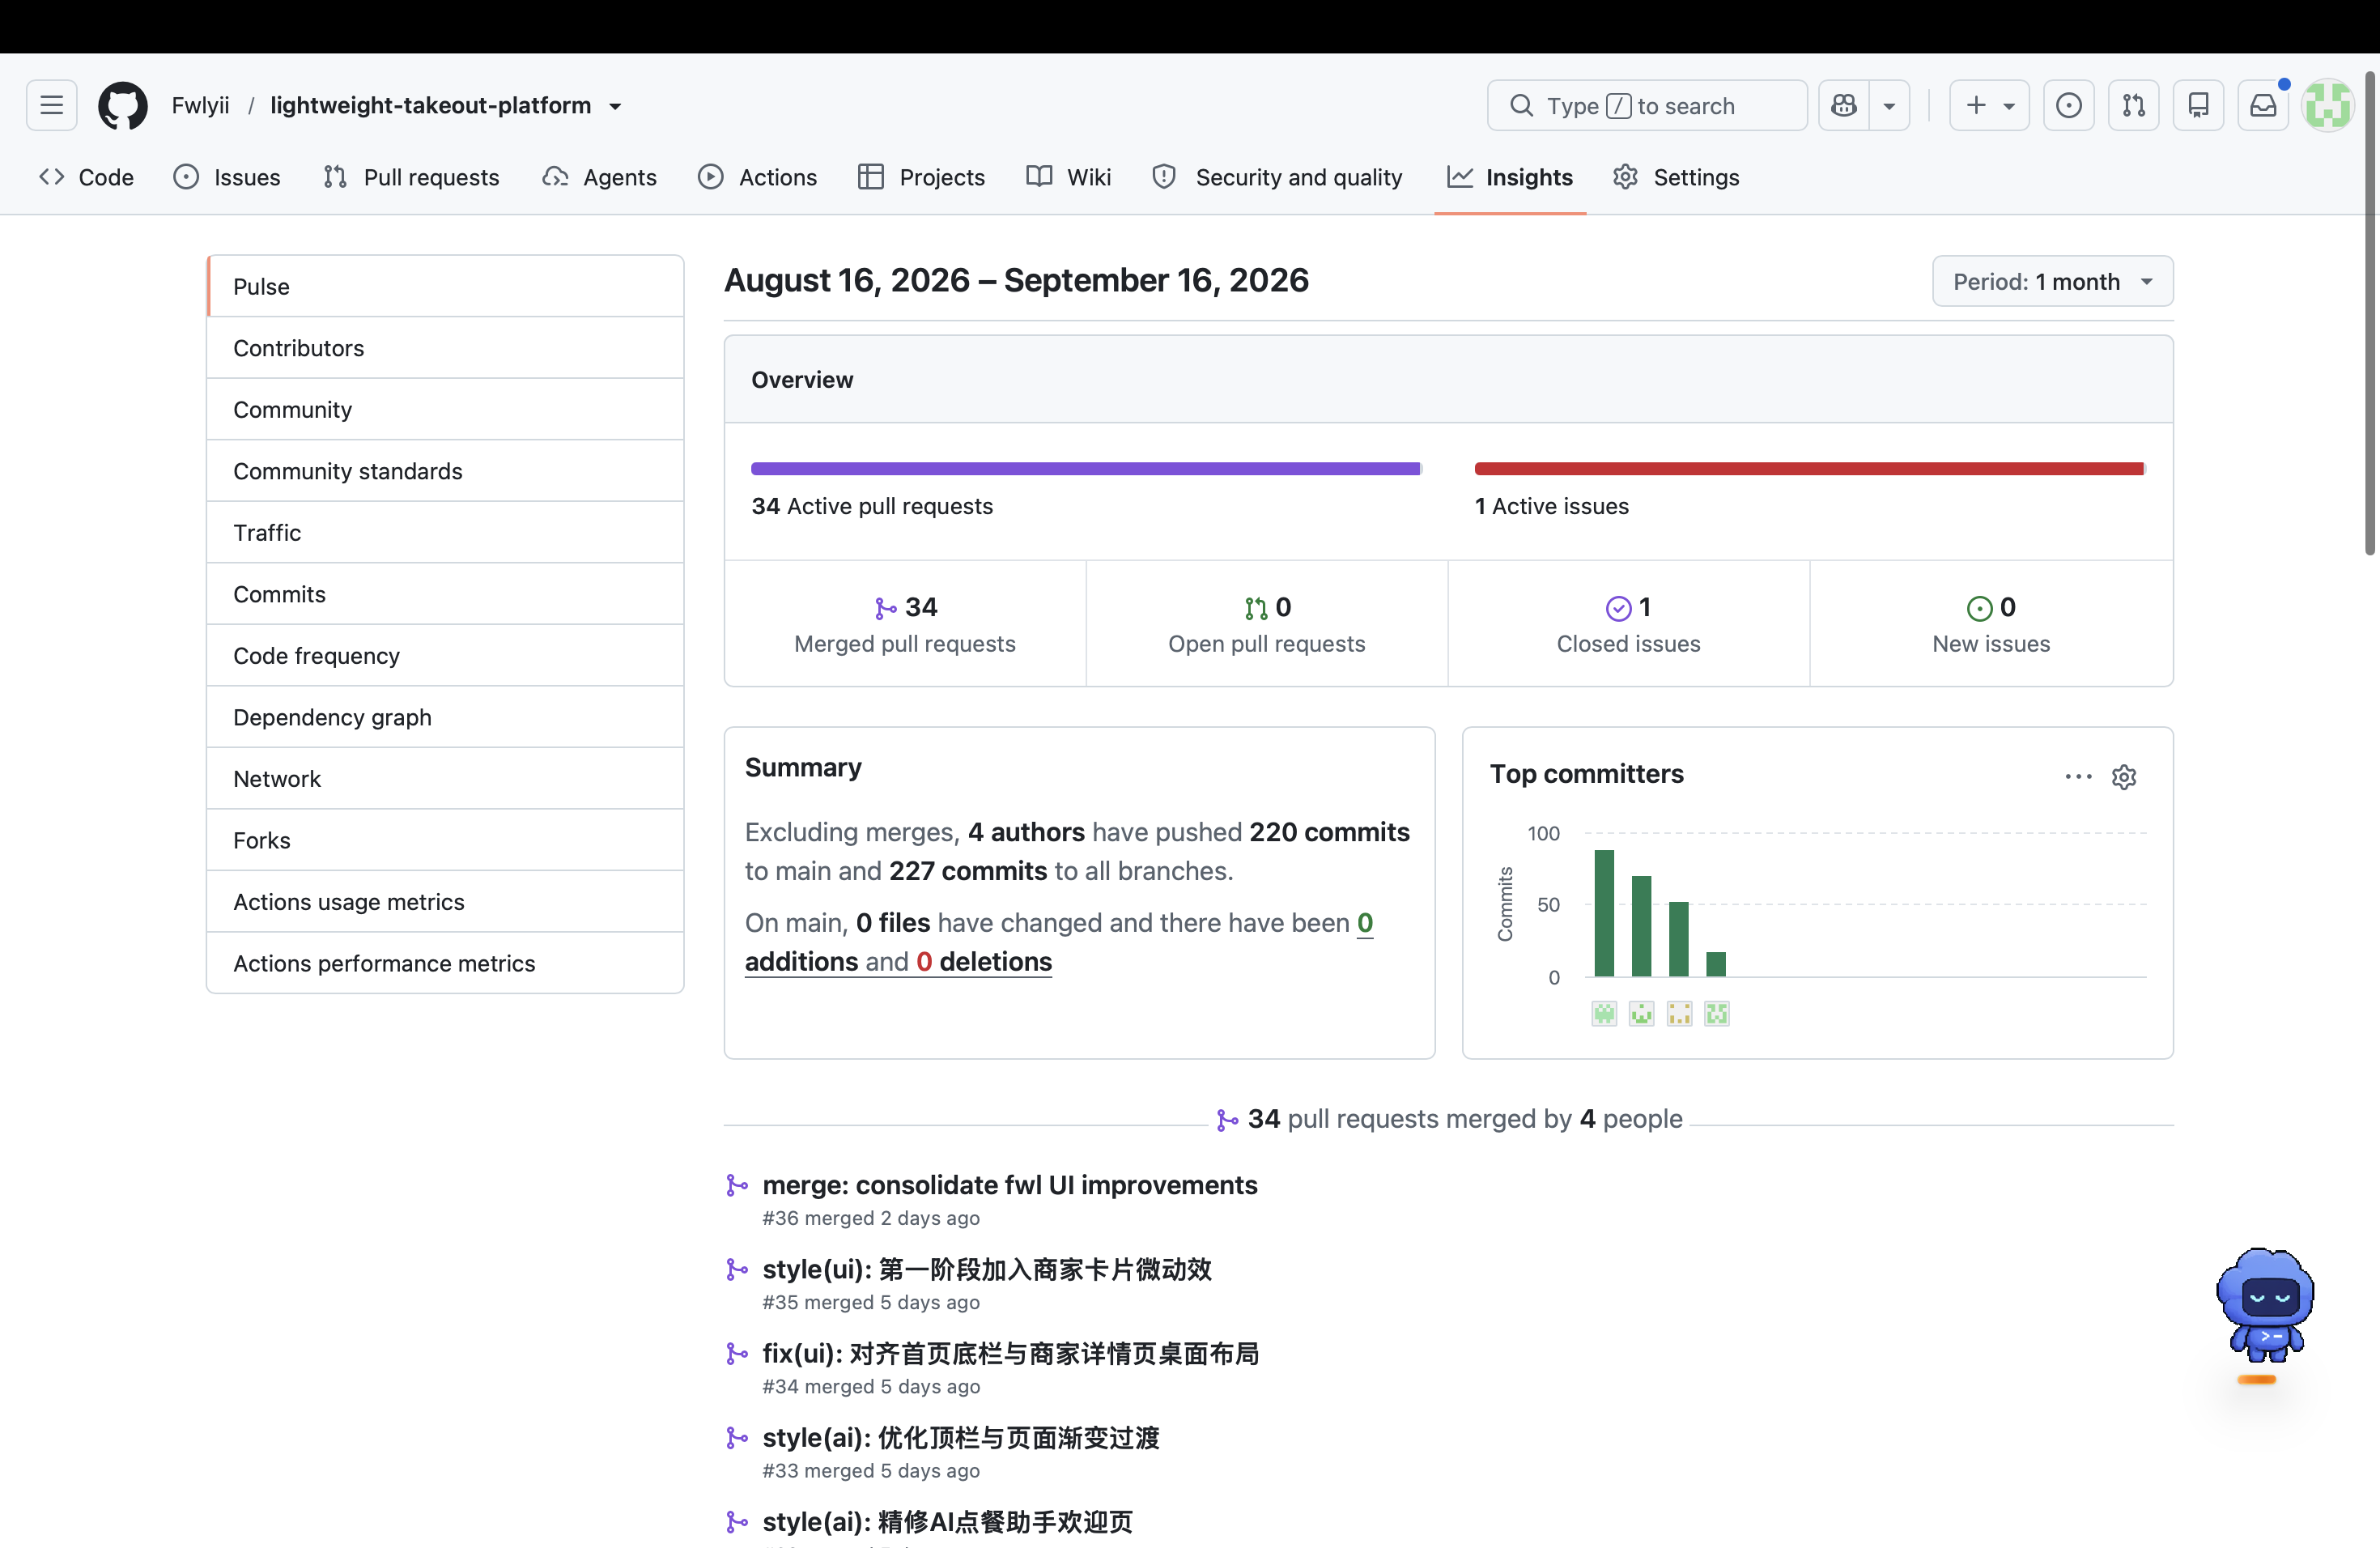
\includegraphics[width=\linewidth,height=.23\textheight,keepaspectratio]{figures/report/process/github-summary.png}
    \captionof{figure}{GitHub 仓库分支合并、提交统计与成员协同全景}\label{fig:proc-gh-summary}
  \end{minipage}\hfill
  \begin{minipage}[t]{.485\linewidth}
    \centering\vspace{0pt}
    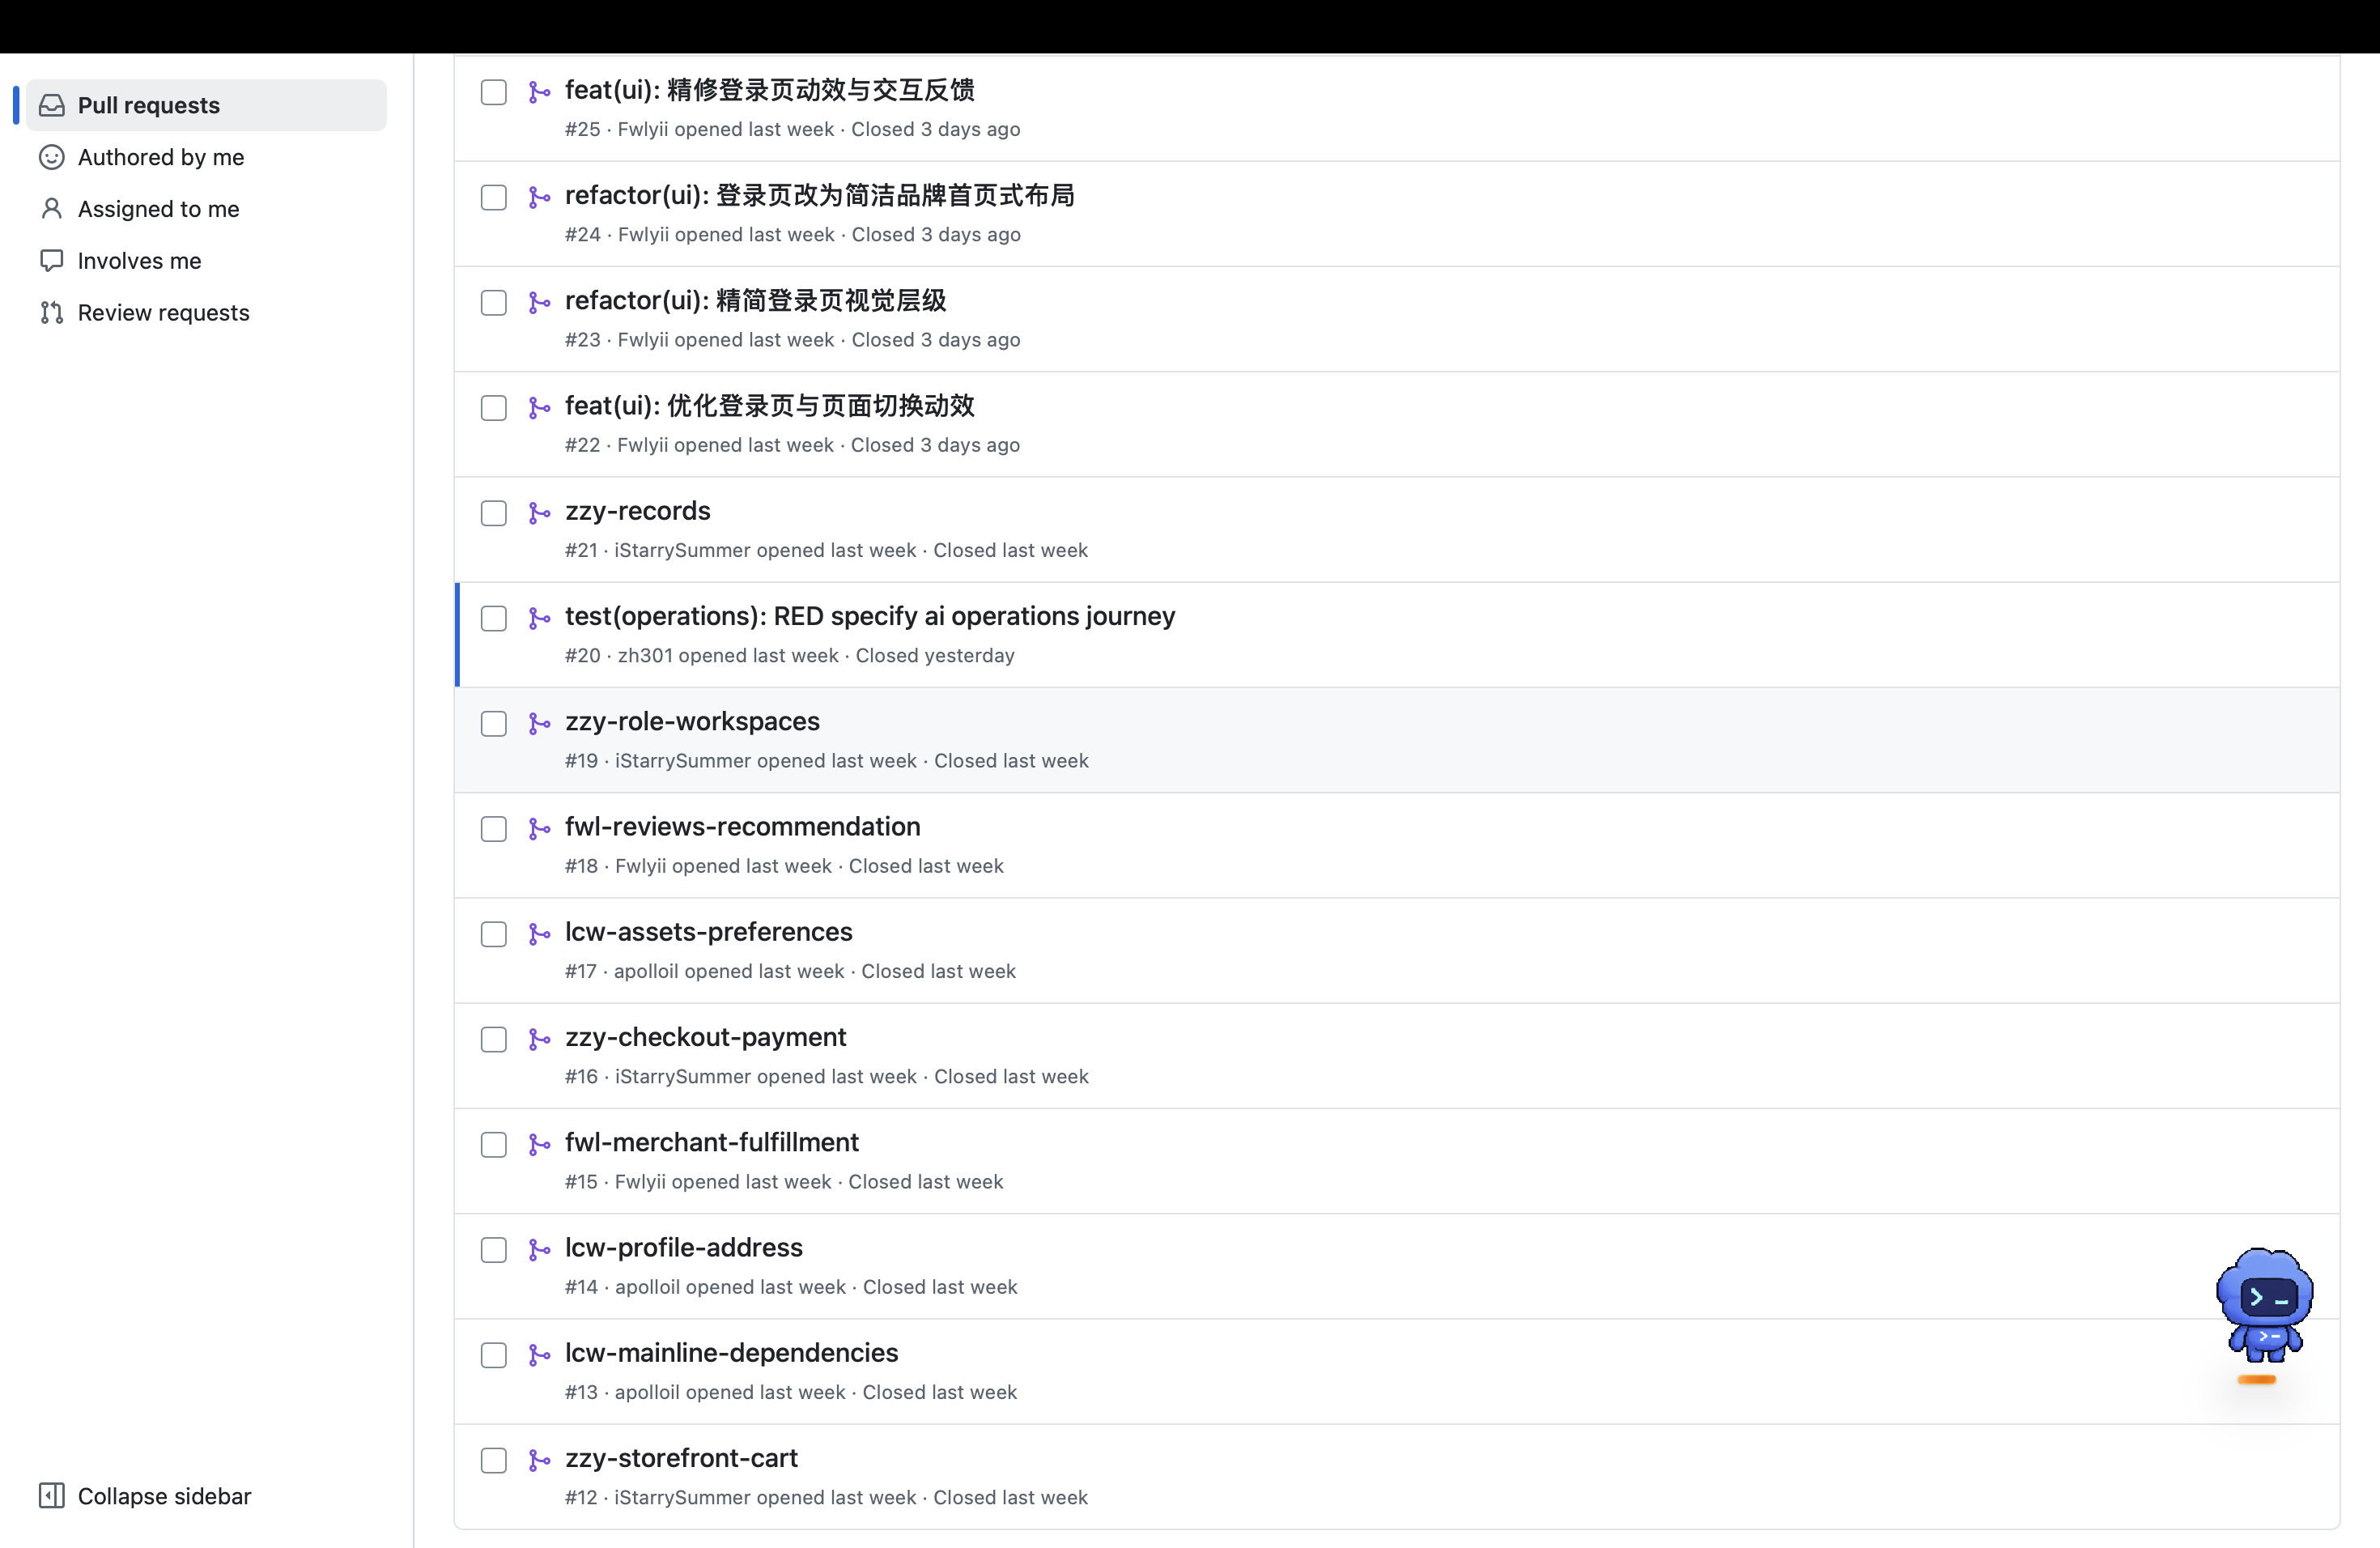
\includegraphics[width=\linewidth,height=.23\textheight,keepaspectratio]{figures/report/process/pull-requests.png}
    \captionof{figure}{团队累计 34 个 Pull Request 评审与合入记录截图}\label{fig:proc-prs}
  \end{minipage}
\end{figure}

GitHub 概览列出 227 条普通提交，其中 220 条进入主分支。全分支统计计入 38 条合并提交，共 265 条。PR 列表按合入请求记录结算支付、商家履约和登录动效等工作，可据此追查具体改动所属的版本。

图~\ref{fig:proc-git-daily} 按日期汇总全分支去重后的提交。9 月 3 日有 60 条，集中于 SRS 和建模。9 月 7 日有 35 条，集中于认证和环境编排。9 月 15 日有 28 条，对应封板整合。用图定位集中修改的日期，再通过 PR 查明改动内容，最后沿同一笔订单走查四端，\mbox{并核对回归结果}。

\begin{figure}[H]
  \centering
  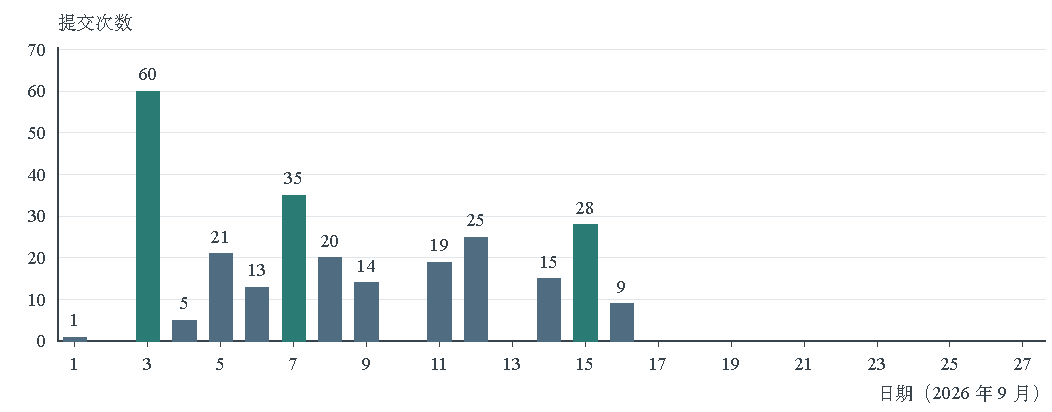
\includegraphics[width=.92\linewidth,height=.32\textheight,keepaspectratio]{figures/report/git-daily.pdf}
  \caption{项目周期每日 Git 提交频次分布统计图（9 月 1 日--9 月 27 日）}
  \label{fig:proc-git-daily}
\end{figure}

  \chapter{项目管理}

排期时，我们先问每轮要交什么、由谁接手、什么时候可以一起联调。这几件事对应课程讲的 4P。产品的范围写进用户故事，人员分工落实到工作包，过程约定接口和验收的顺序，项目层面再跟踪工时、交付日期和风险。跨端接口、交易或外部服务有问题时，我们按它对当轮目标的影响安排修复。

\section{任务计划安排}

\subsection{工作分解（WBS）}

把“顾客能下单”分给一个人，到了联调仍说不清哪一步算做完。我们按 WBS 的“100\% 规则”把需求、测试和交付文档都拆进任务，最小任务尽量安排在 4--8 小时左右。图~\ref{fig:mgmt-wbs-tree} 画出了三层结构。顺着用户故事能找到要完成的改动，手头的任务也能归回当轮交付目标。

\begin{reportpoints}
\item 第一层按需求和工程基础分组，覆盖 \code{US001}--\code{US022} 的 22 个用户故事，以及环境、测试和交付文档。
\item 第二层按 Sprint 列出交付模块，任务编号为 \code{T101}--\code{T308}。接口、数据库、前端与质量工作依实际联调顺序建立依赖。
\item 第三层写明可单独验收的改动，如一项 Controller 接口、一个 SQL 迁移、一个 Vue 组件或一组回归，记录负责人、估算工时和完成标准。
\end{reportpoints}

\begin{figure}[!htbp]
  \centering
  \resizebox{.94\linewidth}{!}{%
\begin{tikzpicture}[
    node distance=0.7cm and 0.45cm,
    root/.style={rectangle,rounded corners=4pt,draw=tjublue,very thick,fill=tjublue,text=white,font=\small\bfseries,minimum width=5.6cm,minimum height=0.9cm,align=center},
    l1/.style={rectangle,rounded corners=3pt,draw=tjublue,thick,fill=lightblue,font=\scriptsize\bfseries,minimum width=2.8cm,minimum height=0.9cm,align=center},
    l2/.style={rectangle,rounded corners=2pt,draw=mutedgray,fill=white,font=\scriptsize,minimum width=2.7cm,minimum height=1.55cm,align=left,inner sep=4pt},
    edge/.style={-{Stealth[length=1.8mm]},thick,tjublue!80}
  ]
    \node[root] (top) {轻量级外卖服务平台项目（230 h 基准 / 118 故事点）};
    \node[l1,below left=1.0cm and 2.5cm of top] (s1) {WBS-1.0 基础设施与\\Sprint 1 核心下单（80 h）};
    \node[l1,below=1.0cm of top] (s2) {WBS-2.0 履约、配送\\与资产闭环（68 h）};
    \node[l1,below right=1.0cm and 2.5cm of top] (s3) {WBS-3.0 管理、AI、地图\\与质量交付（82 h）};

    \draw[edge] (top.south) -- ++(0,-0.45) -| (s1.north);
    \draw[edge] (top.south) -- (s2.north);
    \draw[edge] (top.south) -- ++(0,-0.45) -| (s3.north);

    \node[l2,below=0.55cm of s1] (s1d) {1.1 SRS 与 17 张建模图\\1.2 \code{elm_v2.sql} 与迁移\\1.3 认证、店铺与菜品\\1.4 购物车与幂等下单\\1.5 顾客主链路与单测};
    \node[l2,below=0.55cm of s2] (s2d) {2.1 商家接单出餐管理\\2.2 骑手乐观锁抢单\\2.3 钱包积分券流水账\\2.4 评价、收藏与通知\\2.5 登录视觉与首次联调};
    \node[l2,below=0.55cm of s3] (s3d) {3.1 管理员审核与仲裁\\3.2 多模态 AI 与熔断\\3.3 高德地图与坐标距离\\3.4 四套主题与数据看板\\3.5 575 项回归与容器交付};

    \draw[edge] (s1) -- (s1d);
    \draw[edge] (s2) -- (s2d);
    \draw[edge] (s3) -- (s3d);
  \end{tikzpicture}
}
  \caption{项目三级工作分解结构（WBS）顶层树状图}\label{fig:mgmt-wbs-tree}
\end{figure}

以 \code{T105} 为例，顾客要能提交和取消订单，订单事务因此拆成三个能单独验的工作包。\code{T105-1} 检查优惠、配送费和自取计价，估算 4.0~h。\code{T105-2} 检查扣库存、写快照和防重提交，估算 4.5~h。\code{T105-3} 检查取消时的权限以及库存、资产恢复，估算 3.5~h。三项共 12.0~h，能与 Sprint 1 任务表对上。联调时先跑各自用例，再用一笔完整订单把它们接起来。

在 Sprint 2，\code{T202} 先完成商家接单、拒单和出餐，再接入骑手任务池与乐观锁抢单。两类状态需要在同一笔订单上衔接，所以商家前端和骑手工作台都依赖该模块。在 Sprint 3，\code{T307} 将页面返回回归与云端部署拆成独立任务，前者交付路由测试，后者交付脚本和部署文档。其余任务与依赖见附录~\ref{app:process}，三级拆解示例见表~\ref{tab:wbs-detail}。

\paragraph{跨模块任务的依赖}
前置任务决定哪一天可以联调。Sprint 1 先有数据库基线 \code{T102}，认证和店铺查询才能按同一份数据定义开发。顾客首页对接店铺查询 \code{T104}，购物车结算和订单列表则要等 \code{T105} 可以建单。页面可以先按约定开发，到接口可用时再核对完整操作。

同样的安排用于第三轮。管理员端看板要读取平台统计结果，先排权限与平台治理，再安排统计接口和导出。多模态交互的页面则同结构化助手服务对接，前端主题、动效和页面内容可以并行推进。\code{T308} 的全链路验收排在这几项之后，一次回归可以检查组合在一起的问题。若需要返工，也可沿这张任务表核对由谁负责接口、页面或测试数据。

图~\ref{fig:mgmt-wbs-tree} 的三条分支分别计划投入 80、68 和 82 小时，合计 230 小时。各阶段的工作量也包含测试和交付。首轮在下单功能之后安排单测，第二轮在履约、资产和评价等模块之后集中联调，末轮另外预留全量回归和容器交付的工时。这样核查某项任务时，能同时看到它所在的交付范围和它所依赖的工作。

\subsection{任务估算与偏差分析}

同一项任务，单独写代码和几端联调往往用时不同。我们使用 PERT 三点估算，由主责人与 Scrum Master 给出乐观工时 $O$、最可能工时 $M$ 和悲观工时 $P$，依式~(\ref{eq:pert}) 计算期望工时 $E$ 及标准差 $\sigma$。$O$、$P$ 的权重各为 1，$M$ 的权重为 4。
\begin{equation}\label{eq:pert}
  E = \frac{O + 4M + P}{6}, \qquad \sigma = \frac{P - O}{6}
\end{equation}
以认证、检索、购物车和下单的 \code{T103--105} 为例，表~\ref{tab:pert-estimation} 记录了 24、30、36~h 三种情况，期望 30~h、标准差 2~h，实际用时 31.5~h。这里多用的 1.5~h 是项目总差额 8.0~h 的一部分。三轮计划投入 230.0~h，实际投入 238.0~h，偏差率为 $+3.48\%$。

认证、检索和交易从乐观到悲观相差 12~h，只跑首轮认证和下单测试则相差 4~h。并行工作的几组人能不能拿到同一个可跑的版本，会影响前一组工时。实际超出估算时，我们回任务与联调记录看时间花在哪里，区分一项实现多花了多久，还是几端合起来以后补了检查。

\begin{table}[H]
  \centering
  \caption{核心任务三点估算（PERT）与实际工时偏差对照表}\label{tab:pert-estimation}
  \reporttablesize
  \begin{tabular}{@{}L{.10\linewidth}L{.255\linewidth}C{.07\linewidth}C{.07\linewidth}C{.07\linewidth}C{.09\linewidth}C{.08\linewidth}C{.08\linewidth}C{.09\linewidth}@{}}
\toprule
\textbf{任务} & \textbf{模块摘要} & \textbf{乐观$O$} & \textbf{可能$M$} & \textbf{悲观$P$} & \textbf{期望$E$(h)} & \textbf{标准差$\sigma$} & \textbf{实际(h)} & \textbf{偏差} \\
\midrule
T101--102 & SRS 建模与数据库基线 & 14 & 18 & 22 & 18.0 & 1.33 & 19.0 & +5.6\% \\
T103--105 & 认证、检索、购物车与下单事务 & 24 & 30 & 36 & 30.0 & 2.00 & 31.5 & +5.0\% \\
T106--107 & 顾客首页、详情、地址与结算页 & 18 & 24 & 30 & 24.0 & 2.00 & 24.5 & +2.1\% \\
T108 & Sprint 1 认证与下单测试用例 & 6 & 8 & 10 & 8.0 & 0.67 & 7.5 & -6.3\% \\
T201--203 & 商家履约、骑手抢单与资产服务 & 24 & 30 & 36 & 30.0 & 2.00 & 31.0 & +3.3\% \\
T204--205 & 商家端页面与骑手工作台 & 17 & 22 & 27 & 22.0 & 1.67 & 22.5 & +2.3\% \\
T206--207 & 备注/评价接口与集中联调缺陷单 & 12 & 16 & 20 & 16.0 & 1.33 & 16.5 & +3.1\% \\
T301--303 & 管理治理与多模态 AI 服务 & 22 & 28 & 34 & 28.0 & 2.00 & 29.0 & +3.6\% \\
T304 & 高德地图代理与坐标距离适配 & 8 & 10 & 12 & 10.0 & 0.67 & 10.5 & +5.0\% \\
T305--306 & AI 前端、主题动效与管理看板 & 19 & 24 & 29 & 24.0 & 1.67 & 25.0 & +4.2\% \\
T307--308 & TDD 导航修复与全链路交叉验收 & 15 & 20 & 25 & 20.0 & 1.67 & 21.0 & +5.0\% \\
\midrule
\textbf{合计} & \textbf{三大 Sprint 全周期汇总} & \textbf{179} & \textbf{230} & \textbf{281} & \textbf{230.0} & \textbf{---} & \textbf{238.0} & \textbf{+3.48\%} \\
\bottomrule
  \end{tabular}
\end{table}

\begin{figure}[!htbp]
  \centering
  \begin{minipage}[t]{.46\linewidth}
    \centering\vspace{0pt}
    \resizebox{.98\linewidth}{!}{%
\begin{tikzpicture}[x=1.6cm,y=0.075cm]
    \draw[->] (0,0) -- (5.2,0);
    \draw[->] (0,0) -- (0,78) node[above,font=\scriptsize] {工时 (h)};
    \foreach \y in {0,20,40,60}
      {\draw[gray!25] (0,\y) -- (4.8,\y); \node[left,font=\scriptsize] at (0,\y) {\y};}
    % 李承文
    \fill[tjublue] (0.6,0) rectangle (1.1,68); \node[above,font=\scriptsize] at (0.85,68) {68.0 h};
    \node[below,font=\scriptsize] at (0.85,0) {李承文};
    % 范文丽
    \fill[accentgreen!80!black] (1.6,0) rectangle (2.1,63); \node[above,font=\scriptsize] at (1.85,63) {63.0 h};
    \node[below,font=\scriptsize] at (1.85,0) {范文丽};
    % 赵紫怡
    \fill[accentorange] (2.6,0) rectangle (3.1,56); \node[above,font=\scriptsize] at (2.85,56) {56.0 h};
    \node[below,font=\scriptsize] at (2.85,0) {赵紫怡};
    % 仲禹潼
    \fill[tjublue!55] (3.6,0) rectangle (4.1,51); \node[above,font=\scriptsize] at (3.85,51) {51.0 h};
    \node[below,font=\scriptsize] at (3.85,0) {仲禹潼};
  \end{tikzpicture}}
    \captionof{figure}{四位成员全周期实际投入工时}\label{fig:mgmt-workload}
  \end{minipage}\hfill
  \begin{minipage}[t]{.51\linewidth}
    \centering\vspace{0pt}
    \captionof{table}{各轮成员实际投入工时（h）}\label{tab:member-workload}
    \reporttablesize
    \setlength{\tabcolsep}{3pt}
    \begin{tabular}{@{}lrrrr@{}}
      \toprule
      \textbf{成员} & \textbf{首轮} & \textbf{次轮} & \textbf{末轮} & \textbf{总计} \\
      \midrule
      李承文 & 23.0 & 22.0 & 23.0 & 68.0 \\
      范文丽 & 21.0 & 19.0 & 23.0 & 63.0 \\
      赵紫怡 & 21.5 & 15.0 & 19.5 & 56.0 \\
      仲禹潼 & 17.0 & 14.0 & 20.0 & 51.0 \\
      \midrule
      合计 & 82.5 & 70.0 & 85.5 & 238.0 \\
      \bottomrule
    \end{tabular}
  \end{minipage}
\end{figure}

\paragraph{各轮工时偏差}
Sprint 1、2、3 分别比计划多投入 2.5、2.0 和 3.5~h。首轮增加了历史菜名快照和相应回归，认证与下单测试则比估算少用 0.5~h。第二轮的新增工作主要是新人券判重和登录样式隔离。第三轮集中处理 AI 页返回循环和 375~px 窄屏溢出，并补充相应回归。表~\ref{tab:pert-estimation} 的差额按模块统计，同一次联调涉及的测试和修复也可从迭代记录回查。

表~\ref{tab:member-workload} 列出每轮的实际工作量，图~\ref{fig:mgmt-workload} 给出全周期对比。四人平均投入 59.5~h。李承文、范文丽、赵紫怡和仲禹潼分别占 28.6\%、26.5\%、23.5\% 和 21.4\%。第二轮主要集中在履约和资产联调，第三轮前端与测试的投入有所增加，与当轮看板、响应式统一、地图及交叉验收的安排相符。

\subsection{项目甘特图}

甘特图帮我们看哪几项可以同一天做，哪几项要等前一项。图~\ref{fig:mgmt-gantt} 按三轮的实际时间列了任务，四个里程碑的验收记录见表~\ref{tab:milestones}。

第一轮中，顾客端页面在认证和店铺接口开发期间已开始联调，订单快照与取消事务随后补入主链路。第二轮并行推进商家、骑手和资产服务，联调窗口落在这些任务后半段。图中横条的重叠能用来判断切入联调的时机，里程碑的计划日和验收日则按表~\ref{tab:milestones} 核对。

\begin{figure}[!htbp]
  \centering
  \resizebox{.94\linewidth}{!}{%
\begin{tikzpicture}[x=0.60cm,y=0.62cm]
    % 背景网格与日期刻度 (Day 1 = 9/1 ... Day 19 = 9/19)
    \foreach \d/\lbl in {1/9.1,3/9.3,5/9.5,7/9.7,9/9.9,11/9.11,13/9.13,15/9.15,17/9.17,19/9.19}
      {\draw[gray!25] (\d,0.5) -- (\d,12.5); \node[above,font=\scriptsize] at (\d,12.5) {\lbl};}
    % Sprint 背景分区
    \fill[blue!4] (0.5,0.5) rectangle (7.5,12.5);
    \fill[orange!4] (7.5,0.5) rectangle (12.5,12.5);
    \fill[green!4] (12.5,0.5) rectangle (19.5,12.5);
    \node[font=\scriptsize\bfseries,tjublue] at (4.0,14.8) {Sprint 1（核心闭环）};
    \node[font=\scriptsize\bfseries,accentorange] at (10.0,14.8) {Sprint 2（履约与资产）};
    \node[font=\scriptsize\bfseries,accentgreen] at (16.0,14.8) {Sprint 3（智能治理与验收）};

    % 任务条
    \node[left,font=\scriptsize] at (0.3,11.8) {SRS 建模与表结构};
    \fill[tjublue] (1,11.55) rectangle (3.5,12.05);
    \node[left,font=\scriptsize] at (0.3,10.8) {认证与店铺商品后端};
    \fill[tjublue] (2.5,10.55) rectangle (6,11.05);
    \node[left,font=\scriptsize] at (0.3,9.8) {订单快照与取消事务};
    \fill[tjublue] (4,9.55) rectangle (7.5,10.05);
    \node[left,font=\scriptsize] at (0.3,8.8) {顾客端核心页面联调};
    \fill[tjublue!70] (3.5,8.55) rectangle (7.5,9.05);

    \node[left,font=\scriptsize] at (0.3,7.8) {商家端履约与菜品管理};
    \fill[accentorange] (7.5,7.55) rectangle (11.5,8.05);
    \node[left,font=\scriptsize] at (0.3,6.8) {骑手抢单与配送状态机};
    \fill[accentorange] (8,6.55) rectangle (11.5,7.05);
    \node[left,font=\scriptsize] at (0.3,5.8) {钱包积分优惠券体系};
    \fill[accentorange!75] (8.5,5.55) rectangle (12,6.05);
    \node[left,font=\scriptsize] at (0.3,4.8) {集中联调与 WPS 缺陷单};
    \fill[accentorange!55] (10.5,4.55) rectangle (12.5,5.05);

    \node[left,font=\scriptsize] at (0.3,3.8) {管理端审核与统计看板};
    \fill[accentgreen] (12.5,3.55) rectangle (16.5,4.05);
    \node[left,font=\scriptsize] at (0.3,2.8) {多模态 AI 与高德地图};
    \fill[accentgreen!80] (13,2.55) rectangle (16.5,3.05);
    \node[left,font=\scriptsize] at (0.3,1.8) {TDD 修复与四套主题动效};
    \fill[accentgreen!65] (14.5,1.55) rectangle (17.5,2.05);
    \node[left,font=\scriptsize] at (0.3,0.8) {575 项回归与交叉验收};
    \fill[accentred!75] (16,0.55) rectangle (19.5,1.05);

    % 里程碑菱形
    \draw[fill=tjublue] (3.5,13.55) -- (3.72,13.80) -- (3.5,14.05) -- (3.28,13.80) -- cycle;
    \node[right,font=\scriptsize] at (3.75,13.80) {M1: SRS 2.0};
    \draw[fill=accentorange] (7.5,13.55) -- (7.72,13.80) -- (7.5,14.05) -- (7.28,13.80) -- cycle;
    \node[right,font=\scriptsize] at (7.75,13.80) {M2: MVP};
    \draw[fill=accentgreen] (12.5,13.55) -- (12.72,13.80) -- (12.5,14.05) -- (12.28,13.80) -- cycle;
    \node[right,font=\scriptsize] at (12.75,13.80) {M3: 联调封板};
    \draw[fill=accentred] (19.0,13.55) -- (19.22,13.80) -- (19.0,14.05) -- (18.78,13.80) -- cycle;
    \node[left,font=\scriptsize] at (18.75,13.80) {M4: 交付};
  \end{tikzpicture}
}
  \caption{轻量级外卖服务平台项目实施甘特图与里程碑节点}\label{fig:mgmt-gantt}
\end{figure}

\begin{longtable}{C{.10\linewidth}L{.22\linewidth}C{.13\linewidth}L{.46\linewidth}}
\caption{项目核心里程碑（M1--M4）检查与达成结果表}\label{tab:milestones}\\
\toprule
\textbf{里程碑} & \textbf{里程碑名称} & \textbf{计划/实际日} & \textbf{标志性准出交付物} \\
\midrule
M1 & SRS 2.0 需求冻结 & 9.6 / 9.6 & 17 张 UML/draw.io 建模图、23 张表 DDL 与 22 项用户故事基线。 \\
M2 & MVP 核心链路贯通 & 9.7 / 9.7 & 游客/顾客浏览、购物车、防重提交、取消回滚与登录鉴权跑通。 \\
M3 & 四端全链路联调封板 & 9.15 / 9.15 & 商家/骑手/管理端协同、资产积分体系、AI 多模态与统一壳层合入 \code{main}。 \\
M4 & 验收交付与文档归档 & 9.19 / 9.19 & 575 项全量回归通过、25 项交叉验收证据归档、Docker 一键演示就绪。 \\
\end{longtable}

M1 核定需求和结构，M2 核定可运行的顾客链路。两者间隔一天，因为文档、数据库与认证代码在第一轮并行推进。M2 之后，商家与骑手以已经建立的订单为起点联调。到 M3 时，团队把 AI、主题与四端页面集成在同一版本上，集中修复阻碍操作的问题。M4 再核对回归、交叉证据与演示环境。每个里程碑只检查该阶段应交付的结果，相关依据列在表~\ref{tab:milestones} 中。

\subsection{项目整体燃尽图}

22 项用户故事共 118 个故事点，其中 P0 为 78 点、P1 为 31 点、P2 为 9 点。我们在图~\ref{fig:mgmt-overall-burndown} 上按天记还剩多少点。前期补了 SRS 2.0 的模型和订单菜名快照，收敛稍慢。第二轮把认证、商品和履约主线连起来，9 月 15 日封板后继续验收，9 月 19 日清零。每轮的速率（Velocity）见表~\ref{tab:sprint-velocity}。

\begin{figure}[!htbp]
  \centering
  \resizebox{.86\linewidth}{!}{%
\begin{tikzpicture}[x=0.62cm,y=0.055cm]
    \draw[->] (0,0) -- (20.2,0) node[right,font=\scriptsize] {研发日 (9.1--9.19)};
    \draw[->] (0,0) -- (0,130) node[above,font=\scriptsize] {剩余故事点};
    \foreach \d/\lbl in {1/9.1,3/9.3,5/9.5,7/9.7,9/9.9,11/9.11,13/9.13,15/9.15,17/9.17,19/9.19}
      {\draw[gray!25] (\d,0) -- (\d,120); \node[below,font=\scriptsize] at (\d,0) {\lbl};}
    \foreach \y in {0,30,60,90,118}
      {\draw[gray!25] (0,\y) -- (19.5,\y); \node[left,font=\scriptsize] at (0,\y) {\y};}
    % 理想燃尽线
    \draw[dashed,mutedgray,thick] (1,118) -- (19,0);
    % 实际剩余故事点折线
    \draw[thick,tjublue,mark=*] plot coordinates {
      (1,118) (2,115) (3,108) (4,104) (5,96) (6,88) (7,76)
      (8,68) (9,60) (10,54) (11,45) (12,36) (13,30) (14,22)
      (15,12) (16,6) (17,3) (18,1) (19,0)
    };
    \node[font=\scriptsize,tjublue] at (13.5,95) {— 实际剩余故事点};
    \node[font=\scriptsize,mutedgray] at (13.5,108) {- - 理想燃尽基准线};
  \end{tikzpicture}
}
  \caption{项目全周期整体故事点燃尽图（总计 118 故事点，9 月 1 日--9 月 19 日）}\label{fig:mgmt-overall-burndown}
\end{figure}

到 9 月 7 日，图~\ref{fig:mgmt-overall-burndown} 剩余 76 点，对应首轮交付 42 点。9 月 12 日剩余 36 点，第二轮又交付 40 点。9 月 15 日封板时还剩 12 点，曲线在最后四天逐步收至零。把日线与表~\ref{tab:sprint-velocity} 的迭代汇总对照，可以区分每天的收敛节奏和每轮实际验收的总量。

\begin{table}[H]
  \centering
  \caption{三大 Sprint 敏捷速率（Velocity）与完成率统计表}\label{tab:sprint-velocity}
  \reporttablesize
  \begin{tabular}{@{}L{.18\linewidth}C{.16\linewidth}C{.16\linewidth}C{.16\linewidth}L{.25\linewidth}@{}}
\toprule
\textbf{迭代周期} & \textbf{计划故事点} & \textbf{实际交付点数} & \textbf{迭代完成率} & \textbf{主要交付增量} \\
\midrule
Sprint 1（7 天） & 42 点 & 42 点 & 100\% & SRS 2.0、23 张表基线、认证与下单 MVP \\
Sprint 2（5 天） & 40 点 & 40 点 & 100\% & 商家履约、骑手抢单、资产流水与评价 \\
Sprint 3（7 天） & 36 点 & 36 点 & 100\% & 管理治理、多模态 AI、高德适配与回归 \\
\midrule
\textbf{合计（19 天）} & \textbf{118 点} & \textbf{118 点} & \textbf{100\%} & \textbf{全部 P0/P1/P2 目标交付完毕} \\
\bottomrule
  \end{tabular}
\end{table}

我们把交付多少和用了多久分开看。第二轮 5 天验收了计划的 40 点，实际投入 70.0~h，比计划多 2.0~h。故事点燃尽与实际工时给出了这轮项目的进度和投入。要继续查为什么多花了时间，我们再看过程留下的联调问题、返工和回归记录，如新人券判重和登录样式隔离。这些过程数据有了指向，下一轮估算才能考虑真实发生的工作。

\FloatBarrier
\Needspace{6\baselineskip}
\section{风险评估与规避}

\subsection{风险识别与评估清单}

我们把容易出问题的地方与实际影响记进风险台账。比如模型响应慢会拖长一次调用，订单状态说法不一致则会让几端对同一笔订单给出不同结果。每项分别按高、中、低估计发生概率和影响，再排处置顺序。图~\ref{fig:risk-heatmap} 汇总了 12 项风险，预案见附录~\ref{app:process} 的表~\ref{tab:risk-register}。

\begin{figure}[H]
  \centering
  \resizebox{.72\linewidth}{!}{%
\begin{tikzpicture}[scale=1.0]
    % 3x3 风险热力网格
    \fill[yellow!20] (0,0) rectangle (2.6,1.2);
    \fill[orange!20] (2.6,0) rectangle (5.2,1.2);
    \fill[red!18]   (5.2,0) rectangle (7.8,1.2);
    \fill[green!12] (0,1.2) rectangle (2.6,2.4);
    \fill[yellow!22] (2.6,1.2) rectangle (5.2,2.4);
    \fill[orange!25] (5.2,1.2) rectangle (7.8,2.4);
    \fill[red!18]   (2.6,2.4) rectangle (5.2,3.6);
    \fill[red!30]   (5.2,2.4) rectangle (7.8,3.6);
    \fill[yellow!20] (0,2.4) rectangle (2.6,3.6);

    \draw[gray!60] (0,0) grid[xstep=2.6,ystep=1.2] (7.8,3.6);

    % 轴标签
    \node[left,font=\scriptsize\bfseries] at (-0.1,3.0) {概率：高};
    \node[left,font=\scriptsize\bfseries] at (-0.1,1.8) {概率：中};
    \node[left,font=\scriptsize\bfseries] at (-0.1,0.6) {概率：低};
    \node[below,font=\scriptsize\bfseries] at (1.3,-0.1) {影响：低};
    \node[below,font=\scriptsize\bfseries] at (3.9,-0.1) {影响：中};
    \node[below,font=\scriptsize\bfseries] at (6.5,-0.1) {影响：高};

    % 风险编号分布
    \node[align=center,font=\scriptsize\bfseries,accentred] at (6.5,3.0) {极高风险\\R001};
    \node[align=center,font=\scriptsize\bfseries,accentorange] at (3.9,3.0) {高风险\\R005, R009};
    \node[align=center,font=\scriptsize\bfseries,accentred] at (6.5,1.8) {高风险\\R002, R003, R004\\R007, R010, R011};
    \node[align=center,font=\scriptsize,tjublue] at (3.9,1.8) {中风险\\R006, R008, R012};
  \end{tikzpicture}
}
  \caption{项目 12 项关键风险概率--影响评估矩阵图}\label{fig:risk-heatmap}
\end{figure}

接口、状态含义不一致的 R001 落在高概率、高影响的一格。历史交易数据、库存并发与角色隔离等 6 项是中概率、高影响。模型调用和分支合并列在高概率、中影响一格，联调要给它们留回退或复核的时间。接下来按原编号在表~\ref{tab:risk-closure} 查处理结果和要继续观察的事项。

\subsection{风险跟踪与闭环}

我们把课上讲的风险缓解、监控和管理（RMMM）用在同一张台账里。能提前降低影响的，先定预案；正在发生变化的，留下检查结果；触发后怎么处理，也用原编号记录。交付时，逐项核对 12 项风险的工程处置或持续监控状态，见表~\ref{tab:risk-closure}。

\Needspace{.56\textheight}
\subsection{重点风险的处理与复查}

我们先处理会卡住多端联调的 R001。同一笔订单在顾客、商家和骑手端出现不同含义时，先确认 0--9 的状态对应，再把页面请求、后端 DTO 和契约测试放到一起看，新增接口也同时更新断言。R002、R003 和 R007 从数据上验，分别看历史快照有没有读原值、抢单与库存会不会被重复改动、配送费是否只在外送时计入。

模型调用的 R005 涉及超时和成本。我们以总时限和熔断限制等待，保留本地帮助，继续监控调用预算与限流。地图的 R006 直接用页面验。让地图服务不可用，再看顾客能否继续填写地址并提交订单。离线入口保留后，检查结果同处置状态一起写进风险记录。

交付前我们用风险原来描述的情形复查。权限从四端入口与账号隔离查起，部署在独立环境重启并访问健康端点，范围则回到本期 SRS。R010 提及的真实支付清算和实时 GPS 轨迹列入后续范围，本轮按模拟支付及已约定的履约流程验收。

\paragraph{同一风险的两层检查}
权限相关的 R004 和 R011 分别对应接口与页面。R011 检查各角色从哪一端登录，以及角色与目标路由不匹配时能否得到正确引导。R004 则在服务端确认资源归属，例如同为顾客的两个账号应读取各自的订单与购物车。验收时先走不同角色的页面，再针对同角色的不同账号验证数据。这样可以分清“入口跳转正确”和“后端读取范围正确”各由什么测试覆盖。

R008 的导航风险可以沿完整的返回路径复查。前端用例从原页面打开 AI 主入口，再进入工具页。第一次返回应回到 AI 主入口，第二次返回应回到原页面。用例也覆盖刷新后返回店铺列表，核对查询参数是否保留。页面展示另在窄屏检查，重点看结算按钮和输入框是否仍能操作。这样，修完返回循环后还可以用原用例防止它出现在其他入口。

对交付环境的 R012，代码合入时先检查本机绝对路径、配置文件与挂载路径。独立运行时再确认服务能够启动、健康端点正常，数据库及上传目录能使用准备好的环境配置。配置与运行两个结果分别留在仓库检查和部署验收中，复查时可以判断故障发生在文件打包、容器启动还是服务连接。

演示环境的首次启动可按数据库、迁移、应用的顺序排查。MySQL 就绪后，迁移容器应用订单名称快照和购物车备注两项迁移，成功后以退出码 0 结束。后端在迁移成功后启动，前端通过 Nginx 转发接口请求。首页已打开但订单加载失败时，可按这个顺序查看日志，区分代理转发、数据库连接和迁移故障。

  \chapter{项目交付}

项目交付围绕“软件制品质量验证（测试文档）”与“可复现环境交付（部署文档）”两方面展开。本章基于仓库真实的 53 个后端测试类（340 项）、28 个前端测试文件（235 项）、TDD 红--绿--重构提交链、WPS 人工缺陷筛查台账、本系统四端实机浏览器验证、2026 年 9 月 16 日跨组交叉验收记录及 \code{docker-compose.demo.yml} 容器编排配置，完整记录测试与部署交付物。

\section{项目测试文档}

\subsection{测试计划与测试策略}

\subsubsection{分层测试体系}
本组采用“自动化测试保底线 + TDD 回归防反弹 + 人工四端走查 + 跨组交叉验收”四层质量保障策略：
\begin{enumerate}
  \item \textbf{后端单元测试与集成测试（JUnit 5 + Mockito + MockMvc + H2）：} 共包含 53 个测试类（340 项测试用例），覆盖认证授权边界、请求身份防伪造、订单定价与结算事务、库存条件扣减、历史商品名快照、骑手抢单状态机、AI 意图分流与熔断及高德地图适配器。
  \item \textbf{前端逻辑与源码契约测试（Node Test Runner）：} 共包含 28 个 \code{.test.mjs} 测试文件（235 项测试用例），覆盖购物车备注、结算校验、页面返回导航、高德距离计算、主题切换、接口契约清理与管理端状态逻辑。
  \item \textbf{TDD（红--绿--重构）缺陷驱动实践：} 针对联调中反复出现的“历史订单菜名随商家改价漂移”“未登录/AI 页返回陷入路由死循环”等回归问题，团队严格遵循“先写失败测试（RED）$\rightarrow$ 最小修复通过（GREEN）$\rightarrow$ 集中整理规则（REFACTOR）”三步提交，用自动化断言锁定行为。表~\ref{tab:tdd-trace} 列出了仓库可追溯的 TDD 提交链。
  \item \textbf{人工功能筛查与跨组交叉验收：} 仲禹潼牵头建立 WPS 缺陷登记台账（图~\ref{fig:test-bug-register}），按模块、复现步骤、截图与修复状态闭环管理；9 月 16 日按对照 SRS 功能编号执行跨组交叉验收并留存 24 项页面与边界截图证据。
\end{enumerate}

\begin{longtable}{L{.18\linewidth}L{.14\linewidth}L{.14\linewidth}L{.14\linewidth}L{.31\linewidth}}
\caption{仓库典型 TDD（红--绿--重构）缺陷驱动提交追溯表}\label{tab:tdd-trace}\\
\toprule
\textbf{回归专题} & \textbf{RED（失败）} & \textbf{GREEN（通过）} & \textbf{REFACTOR} & \textbf{固化的工程不变量} \\
\midrule
角色登录权限旅程 & \code{7829525} & \code{eada408} & \code{51b4136} & 角色校验与会话原子发布，失败全回滚。 \\
商家目录管理旅程 & \code{f81c785} & \code{65ae05d} & \code{5212a82} & 跨商家店铺及菜品修改权限严格隔离。 \\
骑手配送状态旅程 & \code{ed0e07a} & \code{99c7c24} & \code{108f5d9} & 抢单并发乐观锁及到店/取餐/送达流转。 \\
资产与偏好旅程 & \code{bff3c7e} & \code{cbd2de8} & \code{401d90d} & 资产流水只增不改，偏好持久化恢复。 \\
订单商品名快照 & \code{3e42fa9} & \code{f4c92ca} & \code{a1af8b7} & 移除实时商品联表，历史单强制读快照。 \\
AI 与页面返回规则 & \code{06780ac} & \code{12c3d6e} & \code{d319c5e} & 集中处理返回兜底，消除未登录死循环。 \\
\end{longtable}

\reportfig[0.96\linewidth]{figures/report/process/bug-register.png}{内部人工功能筛查与缺陷登记台账（WPS 跟踪记录）}{fig:test-bug-register}

\subsection{测试报告}

\subsubsection{自动化测试执行结果汇总}
团队先后于源码快照 \code{17f80ab2} 与 2026 年 11 月 16 日最终文档审计快照 \code{6ddb219} 上执行全量自动化测试套件。2026 年 11 月 16 日在本服务器以 Node.js 22.16.0、OpenJDK 17.0.21 与 Maven Wrapper 重新执行全量回归的结果仍为 \textbf{前端 235 项通过、后端 340 项通过，失败、错误与跳过均为 0（100\% 通过率）}（表~\ref{tab:auto-test-summary}）。

图~\ref{fig:test-terminal-placeholder} 将本次真实日志摘要排版后由浏览器截图，原始前端输出、后端日志摘要及 53 份 Surefire XML 统计归档在 \code{report/evidence/2026-11-16/}。图~\ref{fig:test-domain-dist} 进一步按测试领域可视化展示了 575 项自动化用例的分布情况。

\begin{longtable}{L{.24\linewidth}L{.26\linewidth}C{.12\linewidth}C{.10\linewidth}C{.10\linewidth}C{.10\linewidth}}
\caption{全量自动化测试执行结果汇总表（快照 \texttt{6ddb219} 实测）}\label{tab:auto-test-summary}\\
\toprule
\textbf{测试套件} & \textbf{运行环境与工具} & \textbf{通过数} & \textbf{失败} & \textbf{错误/跳过} & \textbf{通过率} \\
\midrule
后端全量测试（53 类） & OpenJDK 17.0.21 / Maven Surefire / H2 & 340 & 0 & 0 & 100\% \\
前端全量测试（28 文件） & Node.js 22.16.0 / \code{node --test} & 235 & 0 & 0 & 100\% \\
\midrule
\textbf{合计} & \textbf{前后端自动化测试总计} & \textbf{575} & \textbf{0} & \textbf{0} & \textbf{100\%} \\
\bottomrule
\end{longtable}

\begin{figure}[H]
  \centering
  \begin{tikzpicture}[x=0.072cm,y=0.58cm]
    \draw[->] (0,0) -- (125,0) node[right,font=\scriptsize] {用例数};
    \draw[->] (0,0) -- (0,8.2);
    \foreach \x in {0,20,40,60,80,100,120}
      {\draw[gray!25] (\x,0) -- (\x,7.8); \node[below,font=\scriptsize] at (\x,0) {\x};}
    \node[left,font=\scriptsize] at (-1,7.0) {前端导航与安全契约};
    \fill[tjublue] (0,6.7) rectangle (102,7.3); \node[right,font=\scriptsize] at (102,7.0) {102};
    \node[left,font=\scriptsize] at (-1,6.0) {前端下单、定位与主题};
    \fill[tjublue!70] (0,5.7) rectangle (84,6.3); \node[right,font=\scriptsize] at (84,6.0) {84};
    \node[left,font=\scriptsize] at (-1,5.0) {前端 AI 与商家看板逻辑};
    \fill[tjublue!45] (0,4.7) rectangle (49,5.3); \node[right,font=\scriptsize] at (49,5.0) {49};

    \node[left,font=\scriptsize] at (-1,4.0) {后端交易、定价与快照};
    \fill[accentorange] (0,3.7) rectangle (106,4.3); \node[right,font=\scriptsize] at (106,4.0) {106};
    \node[left,font=\scriptsize] at (-1,3.0) {后端认证、权限与边界};
    \fill[accentgreen] (0,2.7) rectangle (82,3.3); \node[right,font=\scriptsize] at (82,3.0) {82};
    \node[left,font=\scriptsize] at (-1,2.0) {后端骑手、管理与审核};
    \fill[accentorange!70] (0,1.7) rectangle (78,2.3); \node[right,font=\scriptsize] at (78,2.0) {78};
    \node[left,font=\scriptsize] at (-1,1.0) {后端 AI 熔断与高德地图};
    \fill[accentgreen!65] (0,0.7) rectangle (74,1.3); \node[right,font=\scriptsize] at (74,1.0) {74};
  \end{tikzpicture}
  \caption{前后端 575 项自动化测试用例按工程域分布统计图}\label{fig:test-domain-dist}
\end{figure}

\placeholderfig[0.92\linewidth]{figures/screenshots/test-terminal-results.png}{前后端测试真实日志摘要（浏览器排版展示）}{实际运行前后端自动化测试后，将本次日志摘要与运行环境一并展示。}{fig:test-terminal-placeholder}

\section{自动化测试结果索引}
2026 年 11 月 16 日的回归在快照 \code{6ddb219} 上运行。后端 53 类共 340 项，前端 28 个文件共 235 项，全部通过。下面列出正文涉及的代表性测试，完整执行明细见 \code{report/evidence/2026-11-16/} 中的 \code{backend-testsuites.json}、\code{backend-tests-summary.txt} 与 \code{frontend-tests.txt}。

\begin{table}[!htbp]
\centering
\begin{minipage}[t]{.48\linewidth}
\centering
\caption{代表性后端测试}\label{tab:all-backend-tests}
\reporttablesize
\begin{tabular}{@{}L{.77\linewidth}R{.15\linewidth}@{}}
\toprule
\textbf{测试类} & \textbf{项数} \\
\midrule
\code{AuthenticationJourneyTest} & 46 \\
\code{OrderNameSnapshotJourneyTest} & 39 \\
\code{ProfileAddressJourneyTest} & 29 \\
\code{AiChatJourneyTest} & 18 \\
\code{AssetServiceTest} & 9 \\
\code{AssistantIntegrationTest} & 8 \\
\code{OrderPricingTrustBoundaryTest} & 1 \\
\code{DeepSeekDeadlineTest} & 1 \\
\bottomrule
\end{tabular}
\end{minipage}\hfill
\begin{minipage}[t]{.48\linewidth}
\centering
\caption{代表性前端测试}\label{tab:all-frontend-tests}
\reporttablesize
\begin{tabular}{@{}L{.77\linewidth}R{.15\linewidth}@{}}
\toprule
\textbf{测试文件} & \textbf{项数} \\
\midrule
\code{navigation.test.mjs} & 42 \\
\code{checkout.test.mjs} & 28 \\
\code{authentication.test.mjs} & 19 \\
\code{assistant-page.test.mjs} & 16 \\
\code{location-picker.test.mjs} & 12 \\
\code{rider-dashboard.test.mjs} & 9 \\
\code{assistant-drawer.test.mjs} & 9 \\
\code{adminAccountApi.test.mjs} & 2 \\
\bottomrule
\end{tabular}
\end{minipage}
\end{table}


\subsubsection{本组系统四端端到端实机验证与缺陷闭环}
为弥补纯单元测试对页面交互渲染覆盖的不足，团队在独立 MySQL 8.0.46 演示数据库环境下启动完整后端与前端服务，围绕“黑盒等价类、边界值、跨角色权限隔离与故障降级”四大维度开展浏览器端到端检查。表~\ref{tab:e2e-own-cases} 汇总了本系统核心 E2E 检查结果，相关实景画面可与第 2 章图~\ref{fig:def-ui-auth} 至图~\ref{fig:def-ui-amap} 互证；内部 WPS 台账及集成回归共闭环修复 12 类核心缺陷（表~\ref{tab:bug-closure}）。

\begin{longtable}{L{.10\linewidth}L{.20\linewidth}L{.38\linewidth}C{.09\linewidth}L{.14\linewidth}}
\caption{本组系统（\texttt{lightweight-takeout-platform}）四端核心 E2E 功能与边界验收表}\label{tab:e2e-own-cases}\\
\toprule
\textbf{用例ID} & \textbf{验证场景} & \textbf{执行步骤与核心检查点} & \textbf{结果} & \textbf{实机佐证} \\
\midrule
\endfirsthead
\multicolumn{5}{c}{{\tablename\ \thetable{} 续表}}\\
\toprule
\textbf{用例ID} & \textbf{验证场景} & \textbf{执行步骤与核心检查点} & \textbf{结果} & \textbf{实机佐证} \\
\midrule
\endhead
\bottomrule
\endfoot
E2E-01 & 四端登录与路由隔离 & 分别使用 \code{demo_user}/\code{demo_merchant}/\code{demo_rider}/\code{demo_admin} 登录；跨端访问受保护路由自动重定向。 & 通过 & 图~\ref{fig:def-ui-auth} \\
E2E-02 & 游客浏览与店铺休息拦截 & 未登录访问 \code{/index} 与 \code{/businessInfo}；查看在售库存，休息状态店铺禁用下单按钮。 & 通过 & 图~\ref{fig:def-ui-cust-browse} \\
E2E-03 & 购物车加购与订单快照 & 加购菜品进入 \code{/cart} 结算；查看 \code{/listDetail} 验证下单菜名快照、单价与状态时间线。 & 通过 & 图~\ref{fig:def-ui-cust-cart-orders} \\
E2E-04 & 钱包资产与主题持久化 & 查看余额 \yen 100.00、1200 积分与 2 张红包；切换“薄荷青”主题后刷新保持生效。 & 通过 & 图~\ref{fig:def-ui-placeholders} \\
E2E-05 & 商家工作台、菜品与接单 & 登录 \code{demo_merchant} 查看店铺列表、菜品库存分类管理、订单面板及顾客评价回复。 & 通过 & 图~\ref{fig:def-ui-merchant-biz}--\ref{fig:def-ui-merchant-orders} \\
E2E-06 & 骑手工作台与任务抢单 & 登录 \code{demo_rider} 查看在线开关、可接任务、收益里程及高德导航入口。 & 通过 & 图~\ref{fig:def-ui-rider} \\
E2E-07 & 管理员看板与三方治理 & 登录 \code{demo_admin} 查看趋势看板、CSV 导出、用户启停、商家审核与骑手/异常仲裁。 & 通过 & 图~\ref{fig:def-ui-admin-home}--\ref{fig:def-ui-admin-users-riders} \\
E2E-08 & 无密钥外部服务优雅降级 & 服务端未配置高德/DeepSeek/DashScope 密钥时，选址展示降级提示，AI 筛选走本地菜单，识菜禁用提示明确。 & 通过 & 图~\ref{fig:def-ui-amap}、图~\ref{fig:ai-runtime-placeholder} \\
\end{longtable}

\begin{longtable}{L{.10\linewidth}L{.26\linewidth}L{.22\linewidth}L{.33\linewidth}}
\caption{核心缺陷发现、根因定位与回归验证闭环记录（BUG-01--BUG-12）}\label{tab:bug-closure}\\
\toprule
\textbf{缺陷编号} & \textbf{缺陷现象} & \textbf{根因定位} & \textbf{修复方案与验证提交} \\
\midrule
\endfirsthead
\multicolumn{4}{c}{{\tablename\ \thetable{} 续表}}\\
\toprule
\textbf{缺陷编号} & \textbf{缺陷现象} & \textbf{根因定位} & \textbf{修复方案与验证提交} \\
\midrule
\endhead
\bottomrule
\endfoot
BUG-01 & 到店自取仍校验起送费与收货地址 & 未区分履约模式的统一计价校验 & 在 \code{OrderPricingService} 与 \code{Cart.vue} 分离自取路径（\code{076b45a}）。 \\
BUG-02 & 未登录进入店铺或 AI 页返回陷入死循环 & 各视图分散调用 \code{router.back()} 缺少回退兜底 & TDD 红-绿-重构（\code{06780ac} $\rightarrow$ \code{12c3d6e} $\rightarrow$ \code{d319c5e}）集中返回规则。 \\
BUG-03 & 连续切页偶发白屏与窄屏登录表单溢出 & 视图转场生命周期异常与登录框固定宽度 & 提交 \code{6a9f3af}、\code{061e7f3} 修复壳层样式与切页守卫。 \\
BUG-04 & 新人优惠券可被重复领取 & 领取接口缺少已领取幂等与唯一判重 & 后端补充优惠券领取次数约束并新增 \code{AssetServiceTest} 断言。 \\
BUG-05 & 语音抽屉关闭后麦克风权限未释放 & 延迟回调触发时未判断抽屉当前激活态 & 提交 \code{ddbeb3a} 在关闭与迟到回调中主动释放音轨。 \\
BUG-06 & 商家修改商品名导致历史订单显示失真 & 旧查询联表读取实时 \code{food.food_name} & 迁移 \code{003} 增加快照列，提交 \code{a1af8b7} 移除联表依赖。 \\
BUG-07 & 骑手并发点击同一任务发生覆盖撞单 & 抢单更新 SQL 缺少状态与版本前置条件 & 在 \code{delivery_task} 引入 \code{version} 乐观锁并新增并发单测。 \\
BUG-08 & 游客访问分类店铺页触发加载异常 & 店铺分类接口未向匿名端放行或字段缺失 & 提交 \code{52be48e} 修复游客浏览与商家分类加载。 \\
BUG-09 & 下单页未配置高德密钥时地址选择阻塞 & 地图选址组件强依赖在线 JS API 初始化 & 提交 \code{74e8dbc} 修复离线区域选择与无密钥文本地址降级。 \\
BUG-10 & 登录页重构样式污染其他路由背景 & 全局样式未做组件作用域或类名隔离 & 提交 \code{7460b46} 移除跨组件全局背景覆盖并新增视觉回归。 \\
BUG-11 & 管理员用户检索快速输入出现旧响应覆盖新结果 & 异步列表请求未做竞态序号丢弃处理 & 提交请求时序保护并由 \code{adminAccountApi.test.mjs} 锁定。 \\
BUG-12 & AI 悬浮球在小视口下超出统一页面壳层边界 & 固定定位参考系脱离共享容器宽度 & 提交 \code{48fd4e3} 收敛至页面壳层内部并新增布局测试。 \\
\end{longtable}

\subsubsection{跨组交叉测试报告（对第 10 组 \texttt{sep-elm} 项目）}
除完成本组系统自测外，2026 年 9 月 16 日团队作为交叉测试方，依据《第十组交叉测试报告》规范对兄弟小组项目 \code{test10}（\code{sep-elm}）按照其 \code{docs/SRS.md} 需求编号逐项开展了本地实机浏览与边界隔离测试（使用独立测试账号用户 A \code{13800000001}、用户 B \code{13800000002} 及商家用户 C \code{13800000003}）。表~\ref{tab:cross-cases} 汇总了该轮跨组交叉测试的代表性检查点，图~\ref{fig:cross-auth-shop} 至图~\ref{fig:cross-isolation} 为 2026 年 9 月 16 日对 \code{sep-elm} 项目实机验收的归档截图证据（注：以下截图测试对象为被测项目 \code{sep-elm}，用于体现本组承担跨组 QA 验收的工程实绩）。

\begin{longtable}{L{.14\linewidth}L{.20\linewidth}L{.38\linewidth}L{.19\linewidth}}
\caption{跨组交叉测试（对 \texttt{sep-elm} 项目）代表性用例与结果汇总表}\label{tab:cross-cases}\\
\toprule
\textbf{对方 SRS 编号} & \textbf{测试模块与账号} & \textbf{验收操作与边界核验要点} & \textbf{验收结论与证据} \\
\midrule
\endfirsthead
\multicolumn{4}{c}{{\tablename\ \thetable{} 续表}}\\
\toprule
\textbf{对方 SRS 编号} & \textbf{测试模块与账号} & \textbf{验收操作与边界核验要点} & \textbf{验收结论与证据} \\
\midrule
\endhead
\bottomrule
\endfoot
FR-USER-01/03/04 & 用户注册、登录与资料（用户 A） & 验证注册防重、错误密码统一拒绝提示、密码长度边界校验与个人资料持久化保存。 & 主流程通过；见图~\ref{fig:cross-auth-shop}、图~\ref{fig:cross-profile-pwd} \\
FR-BIZ/FOOD & 店铺浏览、营业状态与商家端（用户 C） & 验证首页店铺展示、店铺休息状态消费者的拦截提示、商家工作台与店铺资料更新。 & 通过；见图~\ref{fig:cross-merchant}、图~\ref{fig:cross-rest-stock} \\
FR-CART-01/03 & 购物车增删、跨店与清空 & 验证加购合并、跨店加购提示、指定店铺清空及用户 B 跨用户购物车数据隔离。 & 通过；见图~\ref{fig:cross-cart}、图~\ref{fig:cross-isolation} \\
FR-ORDER-01/04 & 订单创建、取消与超库存边界 & 验证生成新订单、待处理订单自助取消、超库存购买拦截及用户 B 跨用户订单隔离。 & 通过；见图~\ref{fig:cross-order}、图~\ref{fig:cross-rest-stock} \\
\end{longtable}

\uitwofig{figures/cross/2026-9-16-sep-elm-SRS验收截图-01-用户首页.png}{（a）被测系统用户首页与店铺列表}{figures/cross/2026-9-16-sep-elm-SRS验收截图-02-店铺商品.png}{（b）被测系统店铺详情与商品展示}{跨组交叉测试（\texttt{sep-elm}）：用户首页与店铺商品验收截图}{fig:cross-auth-shop}

\uitwofig{figures/cross/2026-9-16-sep-elm-SRS验收截图-错误密码登录.png}{（a）错误密码登录拒绝提示}{figures/cross/2026-9-16-sep-elm-SRS验收截图-密码边界.png}{（b）注册/修改密码格式边界拦截}{跨组交叉测试（\texttt{sep-elm}）：认证与密码边界验收截图}{fig:cross-profile-pwd}

\uitwofig{figures/cross/2026-9-16-sep-elm-SRS验收截图-03-购物车.png}{（a）购物车加购与合计状态}{figures/cross/2026-9-16-sep-elm-SRS验收截图-跨店购物车.png}{（b）跨店购物车加购冲突提示}{跨组交叉测试（\texttt{sep-elm}）：购物车功能与跨店冲突截图}{fig:cross-cart}

\uitwofig{figures/cross/2026-9-16-sep-elm-SRS验收截图-04-新订单详情.png}{（a）新订单提交与明细详情}{figures/cross/2026-9-16-sep-elm-SRS验收截图-05-取消订单.png}{（b）订单取消后状态同步与按钮隐藏}{跨组交叉测试（\texttt{sep-elm}）：订单创建与取消闭环截图}{fig:cross-order}

\uitwofig{figures/cross/2026-9-16-sep-elm-SRS验收截图-06-商家工作台.png}{（a）被测系统商家工作台界面}{figures/cross/2026-9-16-sep-elm-SRS验收截图-07-商家订单.png}{（b）被测系统商家订单处理视图}{跨组交叉测试（\texttt{sep-elm}）：商家端工作台与订单验收截图}{fig:cross-merchant}

\uitwofig{figures/cross/2026-9-16-sep-elm-SRS验收截图-消费者侧休息状态.png}{（a）店铺切换休息后消费者侧禁用提示}{figures/cross/2026-9-16-sep-elm-SRS验收截图-超库存边界.png}{（b）超出可用库存下单请求拦截}{跨组交叉测试（\texttt{sep-elm}）：营业状态与超库存边界验收截图}{fig:cross-rest-stock}

\uitwofig{figures/cross/2026-9-16-sep-elm-SRS验收截图-用户B订单隔离.png}{（a）用户 B 登录后订单列表隔离验证}{figures/cross/2026-9-16-sep-elm-SRS验收截图-用户B购物车隔离.png}{（b）用户 B 购物车数据隔离验证}{跨组交叉测试（\texttt{sep-elm}）：跨用户隐私与数据隔离验收截图}{fig:cross-isolation}

\section{项目部署文档}

\subsection{部署架构与环境要求}

系统提供“Docker Compose 一键容器化部署（推荐）”与“Node.js + JDK 17 + MySQL 8 手动开发启动”两种交付方式。图~\ref{fig:deploy-arch} 展示了系统容器化部署拓扑结构：Nginx 静态托管 Vue 3 前端并将 \code{/api} 流量同源反代至 Spring Boot 后端容器，后端连接 MySQL 8 容器并挂载 \code{runtime-uploads/} 持久化媒体文件；可选启用 \code{cloudflared} 临时演示隧道或 Cloudflare Pages 云端部署。

\srsfig[0.95\linewidth]{figures/srs/17-system-deployment.png}{系统容器化部署架构、反向代理与本地/云端交付拓扑图}{fig:deploy-arch}

\subsection{部署步骤与运行配置}

\subsubsection{Docker Compose 一键部署流程}
\begin{lstlisting}[language=bash,caption={Docker Compose 一键演示环境初始化与启动命令}]
# 1. 克隆仓库并进入根目录
git clone --branch main https://github.com/Fwlyii/lightweight-takeout-platform.git
cd lightweight-takeout-platform

# 2. 生成本地 .env 并随机签发 64 位 JWT_SECRET（需 zsh 与 OpenSSL）
zsh scripts/ensure-demo-env.sh

# 3. 构建镜像并启动 mysql、migrate、backend、frontend 服务
docker compose -f docker-compose.demo.yml up -d --build
docker compose -f docker-compose.demo.yml ps -a
\end{lstlisting}

首次启动时，\code{mysql} 服务自动创建 \code{elm_v2} 数据库并按序导入 \code{elm_v2.sql} 与 3 份演示种子脚本；随后一次性容器 \code{migrate} 执行 \code{003_order_name_snapshot.sql} 与 \code{005_cart_order_remarks.sql} 后正常退出（\code{Exited (0)}）；待数据库健康检查通过后，\code{backend} 与 \code{frontend} 启动就绪。

\subsubsection{端口映射、访问入口与演示账号}
表~\ref{tab:deploy-endpoints} 列出了默认本地访问入口、服务职责及内建演示账号体系，表~\ref{tab:deploy-env} 列出了外部增强服务的可选环境变量说明。

\begin{longtable}{L{.22\linewidth}L{.30\linewidth}L{.39\linewidth}}
\caption{默认部署端口、访问入口与演示角色说明}\label{tab:deploy-endpoints}\\
\toprule
\textbf{服务/角色} & \textbf{访问地址 / 演示账号} & \textbf{用途与验证说明} \\
\midrule
前端应用（Nginx） & \url{http://localhost:18081/index} & 四端统一入口，已配置同源反向代理至后端容器。 \\
后端服务（Spring Boot） & \url{http://localhost:18080} & 核心 RESTful API 根地址；Swagger 文档见 \code{/swagger-ui/index.html}。 \\
MySQL 8 数据库 & \code{127.0.0.1:13306}（库 \code{elm_v2}） & 持久化存储 23 张业务表及演示数据，支持本地客户端调试。 \\
演示账号矩阵 & \code{demo_user}、\code{demo_merchant}、\code{demo_rider}、\code{demo_rider_candidate}、\code{demo_admin} & 覆盖顾客下单、商家接单、骑手申请/抢单与管理员审核；多角色测试建议开启独立浏览器会话。 \\
\bottomrule
\end{longtable}

\begin{longtable}{L{.28\linewidth}L{.24\linewidth}L{.39\linewidth}}
\caption{关键环境变量与外部服务降级配置表}\label{tab:deploy-env}\\
\toprule
\textbf{环境变量} & \textbf{默认值 / 示例} & \textbf{作用域与缺失降级说明} \\
\midrule
\code{JWT_SECRET} & 由 \code{ensure-demo-env.sh} 生成 & 必填；后端 JWT 令牌签名密钥，禁止提交至代码仓库。 \\
\code{APP_DEMO_ENABLED} & \code{false}（演示环境为 \code{true}） & 控制模拟钱包充值、模拟支付与体验会员接口开关。 \\
\code{DEEPSEEK_API_KEY} & 空（按需注入） & 启用 AI 文字客服外部模型；未配置时自动降级为本地规则与帮助问答。 \\
\code{DASHSCOPE_API_KEY} / \code{BASE_URL} & 空（按需注入） & 启用 \code{qwen-vl-plus} 图片识菜与 \code{qwen3-asr-flash} 语音草稿；未配置返回 503 并禁用入口。 \\
\code{AMAP_WEB_KEY} / \code{AMAP_JS_KEY} / \code{AMAP_SECURITY_CODE} & 空（后端环境变量注入） & 启用高德 POI 搜索代理、逆地理编码与前端选址弹窗；未配置时降级为离线地址填写。 \\
\bottomrule
\end{longtable}

\subsubsection{非 Docker 本地开发启动与常见故障排查}
若需在无 Docker 守护进程的受限主机直接部署调试：可依次启动用户态 MySQL 8.0 实例并导入 \code{elm_v2.sql}、迁移与演示种子脚本，注入 \code{SPRING_DATASOURCE_URL}、\code{JWT_SECRET} 与 \code{APP_DEMO_ENABLED=true} 后使用 OpenJDK 17 运行 \code{elm_bk-0.0.1-SNAPSHOT.jar}；前端通过 \code{VUE_APP_API_BASE_URL} 指向后端地址并运行 \code{npm run serve}（2026 年 11 月 16 日服务器实机截图与全量回归均采用此隔离模式成功验证）。常见部署与运行故障排查指南见表~\ref{tab:deploy-troubleshoot}。

\begin{longtable}{L{.24\linewidth}L{.32\linewidth}L{.35\linewidth}}
\caption{部署与运行阶段常见故障诊断与排查手册}\label{tab:deploy-troubleshoot}\\
\toprule
\textbf{异常现象} & \textbf{常见根因分析} & \textbf{标准排查与处置步骤} \\
\midrule
后端启动报错 \code{JWT_SECRET} 缺失 & 未执行 \code{ensure-demo-env.sh} 或环境变量未透传至容器 & 重新运行环境脚本生成 \code{.env}，检查 \code{docker compose config} 注入结果。 \\
前端接口报 401 或 CORS 拦截 & \code{VUE_APP_API_BASE_URL} 跨端口未走同源反代或密钥变化 & 确认 Nginx \code{/api} 代理指向或统一前端环境变量，清理浏览器旧 \code{localStorage}。 \\
订单页面显示菜名或备注为空 & 既有旧库未执行增量迁移 \code{003} 或 \code{005} & 按序执行 \code{elm_bk/db/migrations/001--006} 幂等 SQL 脚本。 \\
点击高德选址或识菜报不可用 & 未配置 \code{AMAP_*} 或 \code{DASHSCOPE_*} 密钥 & 属预期安全降级行为，可通过文本地址或“智能筛选”正常点餐，配置密钥后重启生效。 \\
\bottomrule
\end{longtable}

  \chapter{AI 赋能专题}
\definecolor{researchBlue}{HTML}{25465D}
\definecolor{researchTeal}{HTML}{287B78}
\definecolor{researchBronze}{HTML}{B67E33}
\definecolor{researchInk}{HTML}{243348}

开发时，我们请 AI 帮忙整理需求、起草代码和补全测试输入，草稿交回组员逐项复核。系统交付之后，顾客也能从点餐页进入问答、商品推荐、图片识菜和语音点菜。前一项查草稿里的业务规则，后一项查顾客实际看到的商品和订单。

\section{AI 赋能全景架构}

图~\ref{fig:ai-dual-arch} 左侧从 SRS 用例走到人工审查和回归测试。右侧从顾客发出请求开始，系统根据输入选择本地问答、菜单筛选或外部模型，调用出错时再按已有规则返回。

\begin{figure}[!htbp]
  \centering
  \resizebox{.96\linewidth}{!}{\begin{tikzpicture}[x=1pt,y=1pt,
    title/.style={anchor=west,inner sep=0pt,font=\small\bfseries},
    workflow step/.style={inner sep=0pt,anchor=west,align=left,
      font=\linespread{1}\fontsize{9.6bp}{12bp}\selectfont,text=black!88}]
  \foreach \start/\stop/\tone/\name in {
    0/178/researchBlue/{研发过程中的 AI 协作},
    200/422/researchTeal/{点餐流程中的多模态 AI}} {
    \node[title,text=\tone] at (\start,0) {\name};
    \draw[\tone,line width=.84pt] (\start,-12) -- (\stop,-12);
    \foreach \from/\to in {-33/-69,-69/-105,-105/-141} {
      \draw[\tone,line width=.62pt,-{Stealth[length=3.3pt,width=3.1pt]}]
        (\start+4,\from-4) -- (\start+4,\to+5.5);
    }
    \foreach \row in {-33,-69,-105,-141}
      \fill[\tone] (\start+4,\row) circle[radius=2.9pt];
  }
  \node[workflow step] at (16,-33) {补全 SRS 用例并核查差异};
  \node[workflow step] at (16,-69) {SQL 幂等迁移与接口契约核对};
  \node[workflow step] at (16,-105) {生成代码样板与 TDD 边界用例};
  \node[workflow step] at (16,-141) {人工走查与 575 项自动化测试};
  \node[workflow step] at (216,-33) {文字对话与规则问答\\{\textcolor{black!63}{DeepSeek / 本地帮助}}};
  \node[workflow step] at (216,-69) {条件智能筛选\\{\textcolor{black!63}{真实菜单库存 + 一键加购}}};
  \node[workflow step] at (216,-105) {多模态识别\\{\textcolor{black!63}{DashScope 图片识菜 / 语音草稿}}};
  \node[workflow step] at (216,-141) {身份注入、事务外调用、熔断与降级};
\end{tikzpicture}
}
  \caption{项目研发过程与系统运行时双维 AI 赋能全景架构图}\label{fig:ai-dual-arch}
\end{figure}

\section{研发过程全流程 AI 赋能实践}

\subsection{各工程阶段的 AI 协同应用}

整理 SRS 时，人容易顺着成功流程往下写。我们让 AI 帮忙找没交代的分支，比如店铺休息后还能不能加购、库存不足时哪些写入要回滚。产品负责人拿着这些问题去查页面与代码。碰到订单阶段在文档里有两个叫法，就先核准状态值和各端能做的动作，再统一用词。课上讲的需求核查，在这里帮我们把一个模糊的状态词改成了可以逐端检查的条件。

给快照、备注和坐标加列时，我们让 AI 参照已有的 SQL 起草 \code{003}、\code{005} 和 \code{006} 的修改模板。列能否为空、以前的订单能从哪里读数据，留给组员查旧记录后决定。DTO 校验、MyBatis 映射和 CSS 主题变量也可以从草稿开始。合入之前，负责同学回到已有接口和数据，核对字段、权限来源以及旧版本留下的记录。

\subsection{人机协同工作闭环}

给 AI 提任务时，我们会先带上项目现有的 DTO、表结构和业务条件，图~\ref{fig:ai-collab-loop} 左边就是这一步。拿到草稿以后，组员检查身份来源、更新条件、空值和事务的起止，约定应当看到的结果，再运行 \code{./mvnw test} 和 \code{npm test}。管理员检索这类时序问题，AI 能提示几处可疑调用，哪次请求回来得晚，仍要靠浏览器里的复现和写好的用例来确认。

\subsection{人工核查怎样落到代码}

评审 AI 对话控制器时，我们发现 DTO 草稿允许请求写入 \mbox{\code{userId}}。于是将 \mbox{\code{AiChatRequestDTO.userId}} 设为 \mbox{\code{READ_ONLY}}，改由后端从认证上下文取得当前用户。我们也把模型请求移到事务之外，收到回复再写入对话。等待网络响应时，数据库连接仍可供其他请求使用。

我们评审测试草稿时也会追问它最后比较了哪个值。结算接口响应成功以后，还要查清用的是哪一份价格。\code{OrderPricingTrustBoundaryTest} 对照服务端算出的应收金额，检查请求多传的价格字段是否改变结果。图片或语音服务缺少密钥时，后端统一返回 \code{503 FEATURE_UNAVAILABLE}，前端再给出具体提示。这些结果写成断言以后，每次回归都能再查一遍。

\begin{figure}[!htbp]
  \centering
  \resizebox{0.98\linewidth}{!}{%
\begin{tikzpicture}[
    x=1pt,y=1pt,
    review box/.style={rectangle,rounded corners=2.5pt,align=center,
      minimum height=40pt,minimum width=96pt,inner xsep=2pt,inner ysep=3pt,
      draw=researchBlue!66,fill=researchBlue!7,text=researchInk,
      line width=.55pt,font=\fontsize{9.3bp}{13bp}\selectfont},
    arr/.style={-{Stealth[length=4pt,width=3.4pt]},line width=.66pt,draw=researchInk!80}
  ]
    \node[review box] (s1) at (48,0) {\textbf{1. 约束输入}\\锁定 DTO/表/红线};
    \node[review box] (s2) at (155.5,0) {\textbf{2. 辅助产出}\\样板/SQL/用例草稿};
    \node[review box,draw=researchBronze!80,fill=researchBronze!9] (s3) at (263,0)
      {\textbf{3. 人工审计}\\查鉴权/事务/断言};
    \node[review box,draw=researchTeal!75,fill=researchTeal!8] (s4) at (370.5,0)
      {\textbf{4. 门禁验证}\\575 项回归与 PR 合入};
    \foreach \srcnode/\dstnode in {s1/s2,s2/s3,s3/s4}
      \draw[arr] (\srcnode.east) -- (\dstnode.west);
    \draw[arr,densely dashed,draw=researchBronze] (s3.south) -- (263,-37) --
      node[midway,below=2pt,text=researchBronze!80!black,font=\fontsize{8.7bp}{10bp}\selectfont]
        {发现隐式漂移则打回重写} (48,-37) -- (s1.south);
  \end{tikzpicture}
}
  \caption{研发过程四步人机协同审计闭环流程图}\label{fig:ai-collab-loop}
\end{figure}



\section{系统运行时 AI 业务能力设计与落地}

\subsection{多模态 AI 服务矩阵}

顾客从 \code{/ai-chat} 和相应子页面进入助手。想问规则可以直接输入文字，想找菜就给预算和菜名，也可以上传图片或音频。点餐页提供文字对话、规则推荐、图片识菜和语音草稿四个入口，接口、模型及服务不可用时的处理见附录表~\ref{tab:runtime-ai-matrix}。

\subsection{意图分流、安全隔离与熔断降级设计}

顾客问退款规则时，已有的说明就能回答。图片识菜和语音转写则要联系外部服务。图~\ref{fig:ai-guardrails} 把本地与外部调用分别画出来。两条路径都要确认谁在提问、回复可用哪些数据，以及结果返回后要写入什么。

\begin{reportpoints}
  \item 候选菜品来自当前在售且有足够库存的菜单。加购由顾客在卡片上确认，金额仍由购物车和结算接口计算。
  \item 用户 ID 取自认证上下文。订单查询限定在当前用户，待查询的业务内容按数据处理，日志隐藏对话正文。
  \item 模型请求在数据库事务外完成，收到响应后再用短事务写入 \code{ai_chat_history}。
  \item 外部调用受总超时、熔断和重试上限管理。重试上限默认为 3 次。缺少密钥或模型调用失败时，可使用本地帮助与推荐。
\end{reportpoints}

\begin{figure}[!htbp]
  \centering
  \resizebox{0.98\linewidth}{!}{%
\begin{tikzpicture}[
    x=1pt,y=1pt,
    blk/.style={rectangle,rounded corners=2pt,align=center,minimum width=76pt,
      minimum height=39pt,inner xsep=2pt,inner ysep=3pt,line width=.55pt,
      draw=researchBlue!66,fill=researchBlue!7,text=researchInk,
      font=\fontsize{8.6bp}{11.2bp}\selectfont},
    dec/.style={diamond,aspect=1.27,align=center,inner sep=1pt,line width=.55pt,
      draw=researchBronze!86,fill=researchBronze!9,text=researchInk,
      font=\fontsize{8.4bp}{11bp}\selectfont},
    branch/.style={blk,minimum width=112pt,minimum height=38pt},
    arr/.style={-{Stealth[length=3.6pt,width=3.2pt]},line width=.62pt,draw=researchInk!84},
    signal/.style={text=researchInk,fill=white,inner sep=1.5pt,
      font=\fontsize{8.3bp}{10bp}\selectfont}
  ]
    \node[blk] (in) at (38,0) {\textbf{用户多模态输入}\\文本 / 图片 / 语音};
    \node[blk] (ctx) at (127,0) {\textbf{JWT 身份注入}\\剥离伪造 userId};
    \node[dec] (intent) at (215,0) {意图分流\\与密钥检查};
    \node[branch,draw=researchTeal!75,fill=researchTeal!8] (local) at (309,38)
      {\textbf{本地规则 / 订单查询}\\查库真实菜单与本人订单};
    \node[branch,draw=researchBronze!78,fill=researchBronze!8] (ext) at (309,-38)
      {\textbf{脱事务外部调用}\\超时控制 + \texttt{AiCircuitBreaker}};
    \node[blk,draw=researchTeal!75,fill=researchTeal!8] (out) at (416,0)
      {\textbf{结构化候选输出}\\卡片一键加购\\/ 503 降级};

    \draw[arr] (in.east) -- (ctx.west);
    \draw[arr] (ctx.east) -- (intent.west);
    \draw[arr,draw=researchTeal] (intent.north) |- (local.west);
    \node[signal,above right] at (186,38) {本地意图/无Key};
    \draw[arr,draw=researchBronze] (intent.south) |- (ext.west);
    \node[signal,below right] at (186,-38) {外部增强意图};
    \draw[arr,draw=researchTeal] (local.east) -| (out.north);
    \draw[arr,draw=researchBronze] (ext.east) -| (out.south);
  \end{tikzpicture}
}
  \caption{运行时 AI 意图分流、脱事务外部调用与四重安全护栏流程图}\label{fig:ai-guardrails}
\end{figure}

顾客说“某个价格以内想吃什么”时，预算从表单或问题文本取出。推荐服务先用库存筛掉不能买的商品，再把起送差额、配送费和店铺满减算进去，估算最低结算金额。菜单卡片只是推荐结果，顾客点选以后，购物车再按当时的店铺和库存接受加购。

\subsection{从输入到推荐结果}

助手收到文字后，先确认登录用户及会话归属，再根据关键词处理。退款、会员一类疑问从本地规则找答案，提到订单与配送时转到订单对话，给了菜名或预算就从菜单筛。一般对话和订单对话经 \code{AiChatServiceImpl}，模型不可用时由本地分支接手。几种回复共用一个历史服务，重新打开相应会话时仍能读到之前的问答。

\code{AssistantIntegrationTest} 用商品数量、预算和库存来查推荐结果。同时，它也查两张表。推荐完成以后，应新增一条对话历史，购物车保持为空。顾客看完结果后自己决定加购，测试把这条分界固定下来了。相同套件还分别试了未登录访问和跨用户会话，后者在生成回复前就被拒绝。

\subsubsection{文字问答的调用与保存}

图~\ref{fig:ai-chat-history-sequence-uml} 展开 \code{AiChatServiceImpl.chat} 的调用。服务从当前登录会话取用户编号，再核对会话归属。配置了密钥时，服务先尝试让 DeepSeek 生成回复。若没有可用文本，便由本地规则生成答案。这时页面看到的来源也改为本地。

\begin{figure}[!htbp]
  \centering
  \begin{tikzpicture}[
  x=1pt,y=-1pt,
  line width=.46pt,
  annotate/.style={fill=white,align=center,inner sep=1.7pt},
  participant/.style={draw,fill=white,align=center,minimum height=27pt,inner sep=2pt,font=\bfseries},
  activation/.style={draw,fill=white},
  lifeline/.style={dash pattern=on 3pt off 2pt},
  call/.style={-{Stealth[length=4.7pt,width=4.4pt]}},
  reply/.style={dash pattern=on 3pt off 2pt,-{Straight Barb[length=4.4pt,width=4.4pt]}},
  every node/.style={font=\linespread{1}\fontsize{10bp}{11.4bp}\selectfont}
]
  \foreach \x in {27,91,157,236,307,378} {
    \draw[lifeline] (\x,27) -- (\x,304);
  }
  \node[participant,minimum width=49pt,anchor=north] at (27,0) {Web 客户端};
  \node[participant,minimum width=60pt,anchor=north] at (91,0) {\texttt{AiChat}\\\texttt{Controller}};
  \node[participant,minimum width=65pt,anchor=north] at (157,0) {\texttt{AiChatService}\\\texttt{Impl}};
  \node[participant,minimum width=64pt,anchor=north] at (236,0) {\texttt{DeepSeek}\\\texttt{ApiClient}};
  \node[participant,minimum width=63pt,anchor=north] at (307,0) {\texttt{LocalAi}\\\texttt{Responder}};
  \node[participant,minimum width=71pt,anchor=north] at (378,0) {\texttt{AiChatHistory}\\\texttt{Service}};

  \draw (104,109) rectangle (417,161);
  \draw (104,109) -- (135,109) -- (135,119) -- (130,124) -- (104,124);
  \node[font=\bfseries] at (119,116.5) {opt};
  \node[annotate,anchor=west] at (166,118) {[配置了非空白 API 密钥]};
  \draw (104,170) rectangle (417,222);
  \draw (104,170) -- (135,170) -- (135,180) -- (130,185) -- (104,185);
  \node[font=\bfseries] at (119,177.5) {opt};
  \node[annotate,anchor=west] at (166,179) {[\texttt{message == null}]};

  \draw[activation] (87.5,45) rectangle (94.5,294);
  \draw[activation] (153.5,64) rectangle (160.5,276);
  \draw[activation] (374.5,85) rectangle (381.5,100);
  \draw[activation] (232.5,138) rectangle (239.5,154);
  \draw[activation] (303.5,199) rectangle (310.5,214);
  \draw[activation] (374.5,242) rectangle (381.5,259);

  \draw[call] (27,45) -- node[annotate,above] {\texttt{POST /api/ai/chat}} (87.5,45);
  \draw[call] (94.5,64) -- node[annotate,above] {\texttt{chat(request)}} (153.5,64);
  \draw[call] (160.5,85) -- node[annotate,above] {\texttt{requireWritableSession(sessionId)}} (374.5,85);
  \draw[reply] (374.5,100) -- node[annotate,above] {会话写权限校验通过} (160.5,100);

  \draw[call] (160.5,138) -- node[annotate,above] {同步请求模型} (232.5,138);
  \draw[reply] (232.5,154) -- node[annotate,above] {响应或异常} (160.5,154);
  \node[annotate,anchor=west] at (248,140) {取第一候选的非空白正文};
  \node[annotate,anchor=west] at (248,153) {运行时异常时回复仍为空};

  \draw[call] (160.5,199) -- node[annotate,above] {\texttt{reply(request)}} (303.5,199);
  \draw[reply] (303.5,214) -- node[annotate,above] {本地规则回复} (160.5,214);

  \draw[call] (160.5,242) -- node[annotate,above] {\texttt{save(request, response)}} (374.5,242);
  \node[annotate,anchor=east] (saveNote) at (368,249.5)
    {\texttt{@Transactional} 内重校会话并写入记录};
  \draw[densely dotted] (saveNote.east) -- (374.5,249.5);
  \draw[reply] (374.5,259) -- node[annotate,below] {保存正常完成} (160.5,259);

  \draw[reply] (153.5,276) -- node[annotate,above] {回复对象} (94.5,276);
  \draw[reply] (87.5,294) -- node[annotate,above] {成功响应} (27,294);
\end{tikzpicture}

  \caption{文字问答生成、回退与历史保存（UML 时序图）}\label{fig:ai-chat-history-sequence-uml}
\end{figure}

得到回复后，历史服务在单独的事务内重查会话归属，再写入本轮问答。写入完成后控制器才返回成功。联调时可以把回复里标明的来源与同一会话的历史记录对照，分别核对是谁生成了这条回复，以及页面下次打开时能否读回。

\subsection{模型适配与异常回归}

图片里识别出的菜名先拿到平台菜单里匹配，遇到重复的候选就合并。语音转出来的文字则先整理成草稿，留给用户核对菜名和份数。我们在单元测试里给定识别结果。一例返回两份牛肉面，再查候选能不能对上。浏览器里的录音还得考虑人什么时候关闭抽屉。打开后马上关掉，权限回调即使晚到，音轨也要及时释放。

为了单独检查外部调用要等多久，\code{DeepSeekDeadlineTest} 在本机起了一个模拟服务，让它等 3 秒才响应。客户端的总超时为 1 秒，重试上限为 3 次。测试看到调用在总限时内失败，模拟端只收到 1 次正式请求。它把超时后是否继续重试查清了，浏览器上的提示则用来确认用户遇到的是哪种情况。模型和端点配置见表~\ref{tab:runtime-ai-matrix}。

\Needspace{6\baselineskip}
\subsection{演示环境验证}

我们走查的演示环境没有配 DeepSeek 和 DashScope 密钥。打开问答客服能看到欢迎页与快捷问题，切到智能筛选后，输入“鸡腿饭”和 30 元预算，页面从演示库里找出了在售商品。图~\ref{fig:ai-qa-recommend} 记录了本地筛选返回的菜品和加购入口。

\Needspace{.58\textheight}
问答页把提问、历史和快捷入口放在一起。从“20 元内吃什么”这类快捷问题开始，顾客还可以补充要求。智能筛选则用两个表单项保留关键词和预算，拿到结果后仍能看到之前填了什么。图中照烧鸡腿饭是 18.80 元，脆皮鸡腿堡是 19.90 元，与演示菜单上的同名商品一致。每张卡片右侧都能点选加购。

\begin{figure}[H]
  \centering
  \begin{minipage}[t]{.48\linewidth}
    \vspace{0pt}\centering
    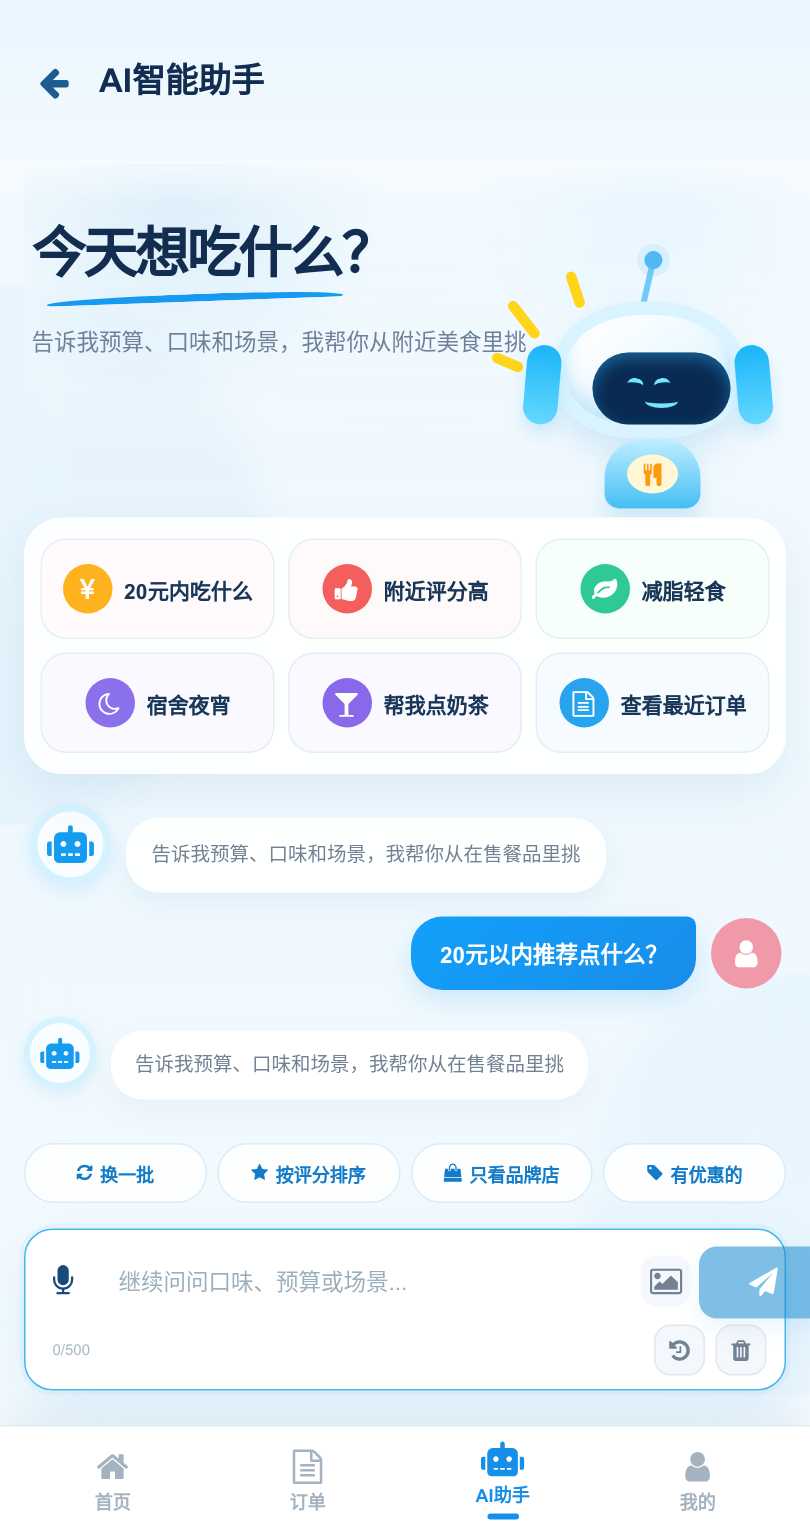
\includegraphics[width=\linewidth,height=.44\textheight,keepaspectratio]{figures/screenshots/ui-ai-chat-qa.png}\par\smallskip
    {\small （a）AI 问答客服入口与快捷提问气泡（\code{/ai-chat}）}
  \end{minipage}\hfill
  \begin{minipage}[t]{.48\linewidth}
    \vspace{0pt}\centering
    
\includegraphics[width=\linewidth,height=.44\textheight,keepaspectratio]{figures/screenshots/ui-ai-assistant.png}\par\smallskip
    {\small （b）智能筛选本地规则推荐结果（真实在售菜单）}
  \end{minipage}
  \caption{AI 智能客服与本地规则推荐界面实景截图（未调用外部大模型）}\label{fig:ai-qa-recommend}\label{fig:ai-runtime-placeholder}
\end{figure}

卡片显示店铺名与商品单价，预算筛选用的却是算上配送和优惠后的最低结算金额。复查时，我们从卡片回到具体店铺和菜品，再对照原来的推荐条件。点了加购之后，还能用购物车里的商品和数量核对下一步。

\clearpage
图~\ref{fig:ai-voice-media} 是语音与图片服务未配置时的页面。我们分别查了录音、文件选择和图片上传入口。这些入口也可以沿用到配置模型后的验收，用于核对浏览器权限和实际识别结果。

页面打开时先请求 \code{/api/v1/assistant/capabilities}。图左的录音和选择音频按钮下方提示语音模型未配置，图右也因缺少识菜模型关闭了图片入口。如果能读到能力状态，就把缺少的那项服务写清楚。如果能力请求本身失败，页面会让用户检查连接，并留出重试入口。

\begin{figure}[H]
  \centering
  \begin{minipage}[t]{.48\linewidth}
    \vspace{0pt}\centering
    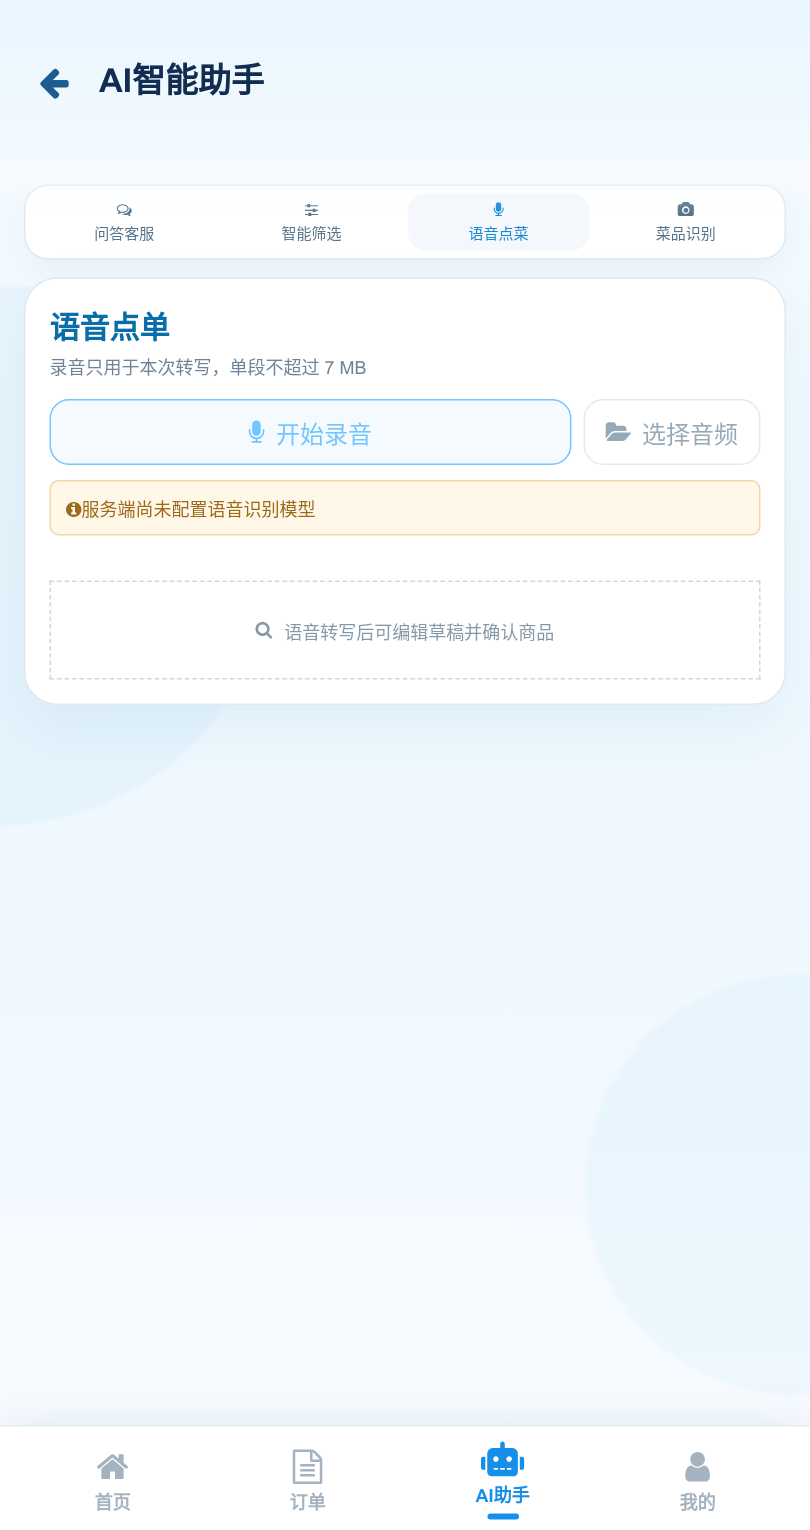
\includegraphics[width=\linewidth,height=.44\textheight,keepaspectratio]{figures/screenshots/ui-ai-voice.png}\par\smallskip
    {\small （a）AI 语音点菜入口与浏览器权限控制（\code{/ai-chat/voice}）}
  \end{minipage}\hfill
  \begin{minipage}[t]{.48\linewidth}
    \vspace{0pt}\centering
    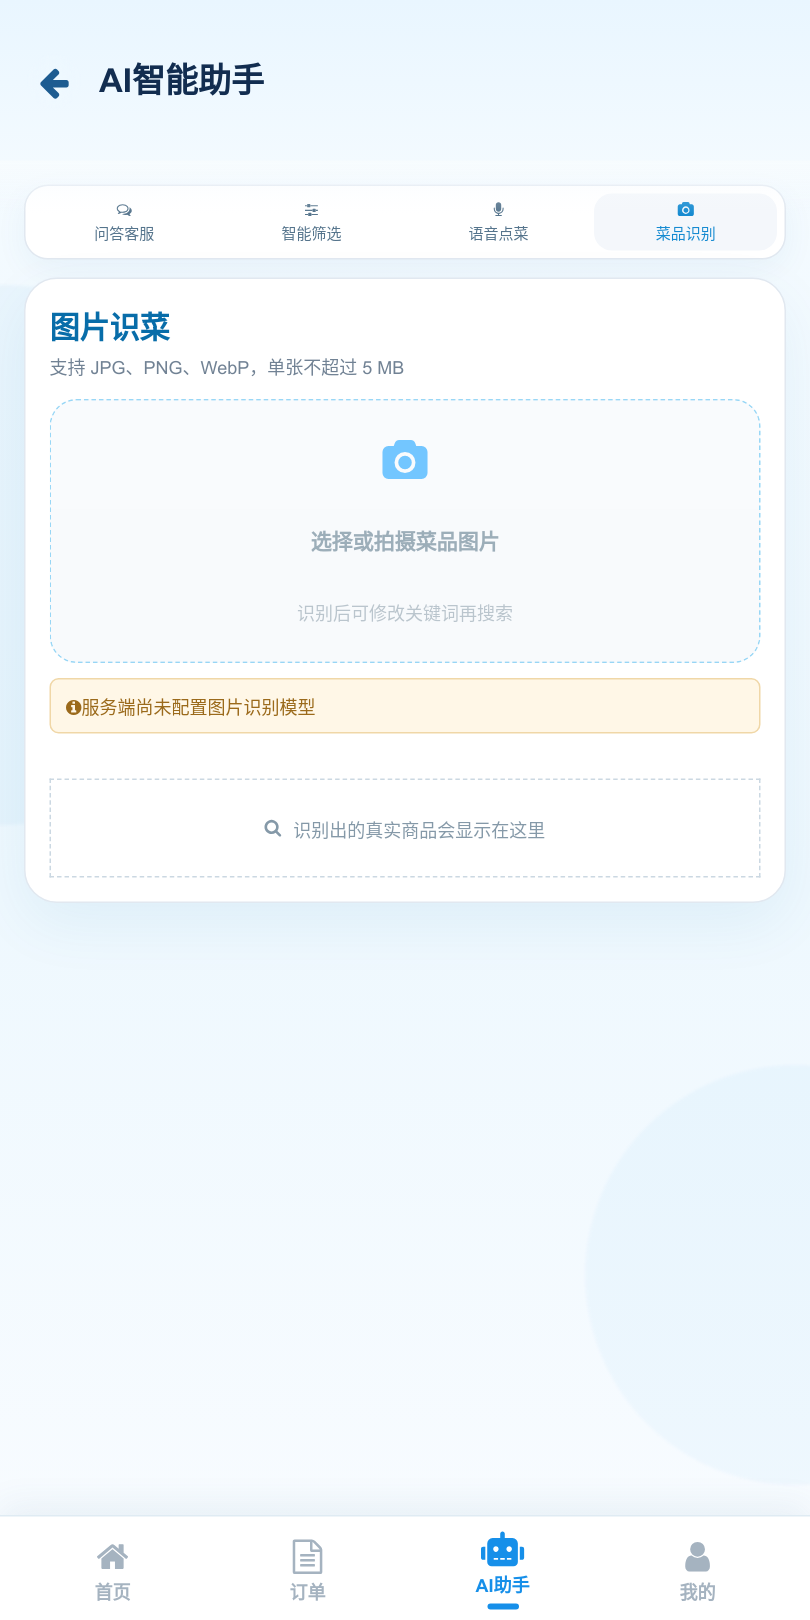
\includegraphics[width=\linewidth,height=.44\textheight,keepaspectratio]{figures/screenshots/ui-ai-media-unconfigured.png}\par\smallskip
    {\small （b）图片识菜模型未配置时的禁用与提示（\code{/ai-chat/image}）}
  \end{minipage}
  \caption{AI 语音点菜与图片识菜未配置降级界面实景截图}\label{fig:ai-voice-media}\label{fig:ai-media-unconfigured}
\end{figure}

接通服务后，语音可以走浏览器授权录音，也可以选本地音频文件。转写出的菜名、份数和预算先放进草稿，顾客改过以后可以重新匹配。图片识菜取出关键词，再列出菜单里的候选。确认具体菜品后，顾客才把它加进购物车。后续验收会从这些动作和页面变化分别检查。

\clearpage
\section{AI 赋能成效评估与核查反思}

\subsection{工程成效评估}

我们用 AI 辅助准备代码样板、SQL 迁移草稿和回归用例。最后交付的是 33 个页面、23 张表和 135 个映射端点，575 项自动化测试均通过。对照历史与现有实现时，我们还找到了 8 项差异，包括订单阶段的叫法和计价顺序。需要继续处理的几项留在表~\ref{tab:gap-improvement}，以后改到相关模块可以回来看。

演示时，顾客在缺少外部模型配置的环境里仍能用本地菜单筛选商品。图片与语音入口依实际状态给出提示，顾客也能返回普通点餐。这是本次走查确认的结果，截图与回归用例分别留住了页面状态和业务判断。

我们在 \code{AssistantIntegrationTest} 里预置了营业和休息的店铺，也给菜品设了不同库存。推荐只返回营业店铺有库存的那一项，对话历史新增一条记录，购物车没有写入。独立推荐接口用同一个预算查两份菜，得到的是空列表。本地退款问答则在历史中标为 \code{local}，模拟历史写入失败后，接口返回服务器错误。这些结果既能从页面找到候选的菜，也能从会话追到产生回复的分支。

\subsection{核查暴露的问题与改进方向}

以后再审阅 AI 草稿，我们会先从一次具体的请求开始。以结算为例，先确认是谁下的单，再看服务端取哪一份价格、最后写下哪些数据。课上讲到，工程师要对交付的结果负责。草稿由谁写并不会改变评审所需的依据，这些字段和断言要由负责该模块的组员核准。

接入有效凭证后，我们计划补测 DeepSeek 对话、DashScope 图片识别和语音转写，记录不同输入的完成率与响应时间。并发时再看单用户 Token 预算、路由调用次数与熔断状态，检查异常请求有没有拖慢普通点餐。未配置画面和超时用例都已留存，可以作为复测的起点。

补测时可以用原来那组菜品、预算与份数。先把能力接口和按钮状态对齐，再逐个试文字、图片与音频，观察识别文本、草稿和候选商品。语音草稿修改份数后再匹配，图片候选可返回具体的店铺菜单。每轮记明服务配置、输入样本与返回状态，耗时按识别、模型生成和菜单匹配分别记录。哪一步失败了，就从该处查起，再确认本地筛选能否继续用。

  \chapter{总结回顾}\label{chap:retrospective}

\section{项目组总结}

项目从四类角色的需求开始，验收时沿这四类角色走完同一笔订单。顾客选择外送或到店自取。外送单由商家接单、出餐，再交给骑手，配送异常由管理员处理。历史订单保留下单时的菜名和地址，模拟支付与退款有对应流水。系统接入地图导航和 AI 点餐，演示时可手工填写地址，也可用本地菜单筛选菜品。交付和验收结果见表~\ref{tab:final-metrics}。

\begin{longtable}{L{.258\linewidth}C{.255\linewidth}L{.448\linewidth}}
\caption{项目最终交付工程指标汇总表}\label{tab:final-metrics}\\
\toprule
\textbf{工程指标维度} & \textbf{实际交付量} & \textbf{可验证仓库依据} \\
\midrule
业务范围与用户故事 & 22 项（\mbox{113 故事点}） & 故事明细按 P0、P1 和 P2 登记。Sprint 计划共 118 点，记录完成率 100\%。 \\
前端视图与后端接口 & 33 视图 / \mbox{24 控制器} & 共 135 个 REST 端点与 4 套 CSS 变量主题 \\
数据库规模与迁移 & 23 张表 / \mbox{6 个迁移} & 含订单快照、资产账本、配送任务版本和地理坐标列 \\
版本协同与代码审查 & 265 提交 / \mbox{34 个 PR} & 覆盖 Sprint 1--3 与文档审计收尾阶段 \\
自动化与实机\mbox{质量验收} & 575 项测试\mbox{全通过} & 后端 340 项（53 类）+ 前端 235 项（28 文件）+ 12 缺陷闭环 \\
\bottomrule
\end{longtable}

排期以 22 项用户故事确定交付范围，一项故事通常涉及多个页面和接口。以配送订单为例，提交时先算金额，履约时再核对订单状态、任务归属和各角色看到的按钮。单元和集成测试验证规则，四端演示从顾客首次操作开始，确认订单能否走到送达。

\subsection{最有帮助的协作做法}

第一次四端联调时，页面都能打开，订单仍会卡在中间。要确认任务能否交给骑手，得回到商家出餐这一步，同时对照顾客看到的状态和骑手的待接列表。后来我们先沿同一笔订单确认状态变化、各页开放操作的条件，再回到各自代码。状态机上的一次转换，由三个角色在各自页面共同核对。

到店自取被起送价拦住时，我们在报错图旁记下履约方式、购物车金额、触发入口和预期结果。前端查结算页，后端查计价分支，测试再按同一条件复测。后来定位旧订单菜名、页面返回和地图缺少配置的问题，也用这套记法。修复人与复测人可以按台账在各自环境中重现问题。

回归和跨组验收把正常下单、接单之外的情形单列为用例，包括取消订单、数量超库存、登录失效和跨账号隔离。文档与实现有差异时，先核对角色、输入和保存结果，再按对应需求确定应补充的规格或代码改动。

\subsection{交付之后的改进顺序}

交付时发现的差异见附录表~\ref{tab:gap-improvement}。后续先统一需求、接口和页面上的订单状态名称，再复跑既有用例。高德和多模态服务接入有效密钥后，沿现有入口补测成功路径，并继续回归离线选址和本地推荐。并发下单和真实支付上线前，分别补测负载、支付回调和对账。已有用例、日志和配置可作为复测起点。

\section{项目组成员总结}

\subsection{范文丽（学号 3024244438）}

我负责前端开发、UI/UX 和数据看板，参与登录、首页、店铺详情、购物车、订单、AI 对话和偏好设置等页面，也维护商家工作台与管理员看板。我设计了清爽蓝白、深海夜色、薄荷青和暖阳橙四套 CSS 变量主题，并实现共享元素转场、响应式页面壳层和统计图表导出。

做登录页和首页动画时，我切到其他路由才发现全局样式也改了背景。屏幕缩到 375~px，登录框会溢出，关闭语音抽屉后音轨有时仍未释放。我们把样式限制在组件内，让动画遵循 \code{prefers-reduced-motion} 设置，再用 \code{theme.test.mjs} 和 \code{assistant-drawer.test.mjs} 复查。后来做看板，我先和后端确认统计口径与空数据展示，再画图。这一轮也让我熟悉了 Vue 3 的页面组织。

\subsection{李承文（学号 3024232129）}

我担任组长和 Scrum Master，负责后端、部署和跨端整合。我管理 GitHub 分支，跟进 34 个 Pull Request 的审查，并搭建 \code{docker-compose.demo.yml} 演示环境。开发任务包括 JWT 鉴权、订单提交事务、服务端计价、多资产结算、骑手配送、管理员治理、导航返回的 TDD 重构和部署解耦。

联调时，一笔取消单要退回资产，两位骑手抢同一单只能有一位成功，顾客在请求超时后重试也只能生成一张订单。我们针对这些情形补充状态前置条件、条件更新和事务，给每次改动留下可重复的测试。四人的课业时间很难排在一起，飞书清单和线上同步明确了阻塞事项和下一位接手者，PR 描述和测试记录也能查到上次改了什么。AI 帮忙写样板和查资料，资金和权限规则由组员共同确定。

\Needspace{7\baselineskip}
\subsection{赵紫怡（学号 3024244137）}

我担任产品负责人，负责需求分析、数据库设计和 AI 点餐开发。我维护 SRS 1.0 和 2.0，绘制系统上下文、参与者、用例和领域类模型，并整理飞书协同空间。我负责 23 张核心表和 \code{001}--\code{006} 增量迁移，参与历史商品名和地址快照设计，并实现 AI 会话、结构化推荐以及 DeepSeek 和 DashScope 的适配与降级。

SRS 的初稿先画正常流程。走查订单和助手时，我和组员补充了商家改名后的历史订单显示、查询他人订单时的助手响应，以及模型响应慢时数据库连接的释放。补上异常流程和状态后，大家可以对着同一操作讨论。多模态助手能把图或语音转成菜名，加购时还需核对菜单、库存和当前用户。和前端、测试一起验这些边界，是我印象最深的部分。

\subsection{仲禹潼（学号 3024244140）}

我负责测试和高德地图服务。内部走查使用 WPS 台账，9 月 16 日跨组验收记录了正常流程与边界场景，报告素材保留了其中 24 张截图。我协助完善前后端自动化回归，负责 POI 搜索、逆地理编码、GCJ-02 距离与送达时间估算、骑手导航，并验证缺少密钥时的处理。

刚接手测试时，我习惯打开页面看哪里有问题。自取卡在起送价、新人券可以重复领、游客点击返回又绕回原页，这几次让我发现，复现时必须写清账号角色和上一步操作。测地图也一样。坐标缺失时，从选址页查地址能否填写，从配送页查骑手能否读到文字地址。开发同学按记录复现，回归时也能据此分辨权限、数据和第三方服务的问题。

\paragraph{交付材料与复现}
归档时，团队将验收所用的源码版本 \code{6ddb219} 和运行环境记入 \code{verification.json}，将操作编号与截图一同保留。前端测试输出和后端测试摘要提供相应断言，台账记录已修缺陷的原因与提交。

复验可从顾客下单、商家接单、骑手接任务一直走到收货，记录各页状态。随后单独检查自取的费用和地址，以及历史明细中的菜名。把版本、账号角色和操作前后的状态一起归档，接手者就能按同样条件复测。这是我们希望继续保持的做法。需求写清楚，问题能复现，修复后留下一次还能运行的测试。

  \appendix
  \titleformat{\chapter}{\centering\hei\bfseries\fontsize{18bp}{21.6bp}\selectfont}{附录\ \thechapter}{1em}{}
  \renewcommand{\thetable}{\thechapter-\arabic{table}}
  \renewcommand{\thefigure}{\thechapter-\arabic{figure}}
  \renewcommand{\theequation}{\thechapter-\arabic{equation}}

  \chapter{项目范围与工程基线}\label{app:project}
  \section{迭代就绪与完成准则}

\begin{table}[H]
\centering
\caption{迭代就绪与完成检查项}\label{tab:dor-dod}
\begin{minipage}[t]{.48\linewidth}
\reporttablesize
\begin{tabularx}{\linewidth}{@{}Y@{}}
\toprule
\textbf{进入迭代（DoR）} \\
\midrule
故事写清角色、使用目标、业务价值及 MoSCoW 优先级。 \\
表结构有变更时，先确定迁移方案。 \\
前后端对齐请求路径、DTO 字段与状态码。 \\
\midrule
查阅飞书待办列表、SRS 用例和 \mbox{SQL 评审记录。} \\
\bottomrule
\end{tabularx}
\end{minipage}\hfill
\begin{minipage}[t]{.48\linewidth}
\reporttablesize
\begin{tabularx}{\linewidth}{@{}Y@{}}
\toprule
\textbf{验收完成（DoD）} \\
\midrule
运行 \code{./mvnw test} 和 \code{npm test}，覆盖主流程与\mbox{关键边界。} \\
人工复核身份提取与权限注解。 \\
PR 合入 \code{main} 后能正常启动容器，缺陷在 WPS 台账复测关闭。 \\
\midrule
查阅 PR、Surefire/Node 日志和缺陷台账。 \\
\bottomrule
\end{tabularx}
\end{minipage}
\end{table}

\section{用户故事与验收条目}

表~\ref{tab:product-backlog} 保留 22 项用户故事与 SRS 用例的对应关系，优先级汇总见表~\ref{tab:backlog-summary}。

\begin{longtable}{@{}L{.071\linewidth}L{.153\linewidth}L{.275\linewidth}C{.145\linewidth}L{.309\linewidth}@{}}
\caption{用户故事与验收条件}\label{tab:product-backlog}\\
\toprule
\textbf{编号} & \textbf{SRS 用例} & \textbf{角色与目标} & \textbf{\mbox{优先级 / 点数}} & \textbf{重点验收条件} \\
\midrule
\endfirsthead
\multicolumn{5}{c}{{\tablename\ \thetable{} 续表}}\\
\toprule
\textbf{编号} & \textbf{SRS 用例} & \textbf{角色与目标} & \textbf{\mbox{优先级 / 点数}} & \textbf{重点验收条件} \\
\midrule
\endhead
\bottomrule
\endfoot
US001 & UC-COM-01 & 用户注册、登录、\mbox{修改资料及退出。} & P0 / 5 & 用户名和手机号唯一。拒绝错误密码与停用账号，登录\mbox{后使用 JWT。} \\
US002 & UC-COM-02/03 & 已登录用户申请商家或\mbox{骑手角色。} & P0 / 5 & 服务端决定角色，审核结果进入站内消息，可标为已读。 \\
US003 & UC-CUS-01 & 游客或顾客分类检索、排序并\mbox{浏览店铺及菜品。} & P0 / 5 & 游客可浏览。\newline 休息店铺不可加购。\newline 售罄或下架菜品不可下单。 \\
US004 & UC-COM-02 & 顾客管理\mbox{收货地址及}\mbox{默认地址。} & P0 / 3 & 仅本人可读写，校验 11 位手机号，默认地址唯一。 \\
US005 & UC-CUS-02 & 顾客按店管理购物车、备注及勾选项。 & P0 / 8 & 同一商品合并数量，校验库存与限购，结算后\mbox{保留未选商品。} \\
US006 & UC-CUS-03/04 & 顾客选择外送或自取，试算后提交订单。 & P0 / 8 & 自取免配送费、起送价和地址要求，幂等键防重，\mbox{库存条件扣减。} \\
US007 & UC-CUS-04/05 & 顾客追踪、取消\mbox{或确认订单。} & P0 / 5 & 仅可访问本人订单。取消恢复库存并退资产，\mbox{确认后发放积分。} \\
US008 & UC-CUS-06 & 顾客评价、查看回复、\mbox{点赞和收藏。} & P1 / 5 & 一单一评，评分 1--5 星，可上传最多 3 张图。收藏\mbox{列表可维护。} \\
US009 & UC-MKT-01 & 顾客使用模拟钱包、优惠券、会员和积分。 & P1 / 8 & 支持新人券和 30 天体验会员，金额以 \code{BigDecimal} 运算，资产\mbox{变更写流水。} \\
US010 & UC-PER-01 & 顾客切换主题并\mbox{设置偏好。} & P1 / 3 & 4 套主题即时切换，辣度、口味和忌口持久化，可\mbox{恢复默认设置。} \\
US011 & UC-MER-01 & 商家申请开店并\mbox{配置店铺。} & P0 / 5 & 维护本人审核通过的店铺及价格规则。休息状态下\mbox{禁止新下单。} \\
US012 & UC-MER-02 & 商家维护商品、分类、\mbox{库存和上架。} & P0 / 5 & 改名改价保留历史快照，单笔限购与库存校验有效。 \\
US013 & UC-MER-03 & 商家接单、拒单和\mbox{确认出餐。} & P0 / 5 & 拒单退资产并恢复库存。出餐后外送进入任务池，\mbox{自取进入待取餐。} \\
US014 & UC-MER-04 & 商家回复评价，查看及导出经营报表。 & P1 / 5 & 仅回复本店评价，按日期查看已完成订单的营收与\mbox{热销趋势。} \\
US015 & UC-RID-01/02 & 骑手申请入驻，\mbox{上线后抢单。} & P0 / 5 & 审核通过后可上线。系统只更新待接且未分配的任务，\mbox{一人领取成功。} \\
US016 & UC-RID-03/04 & 骑手记录到店、取餐、\mbox{送达并导航。} & P0 / 5 & 同步订单状态及节点时间，缺坐标时显示文本地址。 \\
US017 & UC-ADM-01 & 管理员审核商家、\mbox{店铺和骑手。} & P0 / 5 & 审核意见和站内通知可追溯，无权限请求返回 403。 \\
US018 & UC-ADM-02 & 管理员管理账号、评价并\mbox{查看订单。} & P0 / 5 & 停用账号受访问限制。隐藏评价从前台撤下并\mbox{保留后台记录。} \\
US019 & UC-AI-01 & 顾客咨询订单并获取\mbox{菜品推荐。} & P1 / 5 & 查询限于本人订单，候选取自在售菜单，顾客确认后才\mbox{加购或下单。} \\
US020 & UC-AI-02 & 顾客用语音或\mbox{图片辅助点餐。} & P2 / 5 & 外部调用位于事务外。配置缺失时给出提示，普通点餐\mbox{仍可使用。} \\
US021 & UC-RID-04 / ADM-02 & 骑手上报异常，\mbox{管理员仲裁。} & P0 / 4 & 异常挂起订单（状态 9），可恢复、改派或\mbox{终止并回退资产。} \\
US022 & UC-ADM-03 / CUS-06 & 管理员查看平台趋势，顾客查看消费统计。 & P1 / 4 & 平台按时间统计成交、店铺和订单，个人消费\mbox{按月或年汇总。} \\
\end{longtable}

联调时可以按一笔订单查阅这张表。顾客提交外送订单先看 US006，商家接单和出餐看 US013，骑手领取任务及送达分别看 US015 和 US016。同一订单到了下一端，还要核对编号、当前状态和可执行动作是否一致。遇到取消或配送异常时，可回查 US007 和 US021，明确发起方及其对应的库存或资产处理，再用表~\ref{tab:state-mapping} 核对订单何时挂起，何时可以恢复或终止。

\section{技术栈与架构风险}

\begin{table}[H]
\centering
\begin{minipage}[t]{.48\linewidth}
\reporttablesize
\caption{技术选型}\label{tab:tech-stack}
\begin{tabularx}{\linewidth}{@{}L{.25\linewidth}Y@{}}
\toprule
\textbf{层级} & \textbf{组件与用途} \\
\midrule
前端 & Vue 3、Vue Router 4、Axios、CSS 变量分别承载页面、鉴权路由、请求和主题。 \\
后端 & Java 17、Spring Boot 3.4.6、Spring Security 与 JJWT 处理业务和认证，WebSocket 推送状态。 \\
持久化 & MySQL 8.0、MyBatis、HikariCP 支持条件更新与快照写入。 \\
外部调用 & DeepSeek、DashScope、高德 Web/JS API 支持对话、\mbox{多模态及选址。} \\
验证交付 & Vue CLI、Node.js Test Runner、JUnit 5、Mockito、MockMvc 和 H2 用于构建与测试。Docker Compose 和 Nginx 用于交付。 \\
\bottomrule
\end{tabularx}
\end{minipage}\hfill
\begin{minipage}[t]{.48\linewidth}
\reporttablesize
\caption{架构风险与处理方式}\label{tab:init-risk}
\begin{tabularx}{\linewidth}{@{}L{.36\linewidth}Y@{}}
\toprule
\textbf{风险} & \textbf{设计处理} \\
\midrule
计价与身份 & 价格由服务端查库重算，身份取自 JWT 上下文。 \\
外部调用慢 & AI 服务先请求外部模型，再短事务落库。 \\
库存与抢单 & 按可用库存扣减。领取任务时检查状态及骑手归属，成功后递增任务版本号。 \\
前端升级 & 保留兼容接口，委托同一业务服务，契约测试\mbox{覆盖返回结构。} \\
\mbox{地图与模型配置} & 选址失败时可手填地址，推荐链路保留本地筛选。 \\
\bottomrule
\end{tabularx}
\end{minipage}
\end{table}

\section{订单状态编码}

表~\ref{tab:state-mapping} 对照订单枚举 0--9、跨端业务阶段与触发条件。

\begin{longtable}{C{.068\linewidth}L{.196\linewidth}L{.196\linewidth}L{.49\linewidth}}
\caption{源码订单状态编码（0--9）与跨端业务口径映射表}\label{tab:state-mapping}\\
\toprule
\textbf{编码} & \textbf{当前实现名称} & \textbf{对应履约阶段} & \textbf{流转触发条件与业务规则} \\
\midrule
\endfirsthead
\multicolumn{4}{c}{{\tablename\ \thetable{} 续表}}\\
\toprule
\textbf{编码} & \textbf{当前实现名称} & \textbf{对应履约阶段} & \textbf{流转触发条件与业务规则} \\
\midrule
\endhead
\bottomrule
\endfoot
0 & 待支付 & 订单建立 & 提交订单成功后生成。支持顾客支付或取消。超时 15 分钟自动取消并恢复库存。 \\
1 & 待商家接单 & 支付完成 & 支付成功触发。商家可执行接单或拒单，顾客在接单前可取消并全额退还资产。 \\
2 & 待派单\mbox{（制作中）} & 商家备餐 & 商家接单后进入。备餐完成后外送推入骑手池（3），自取进入待取餐（4）。 \\
3 & 待骑手接单 & 骑手抢单池 & 外送出餐后对在线骑手可见，仅首个通过条件更新的骑手可绑定成功。 \\
4 & 待取餐 & 到店交接/\mbox{自取待取} & 骑手接单/到店，或自取订单出餐完成后进入。自取由顾客直接核销取餐。 \\
5 & 配送中 & 外送在途 & 骑手确认取餐后进入，同步记录 \code{pickup_time}。 \\
6 & 已送达 & 待确认收货 & 骑手确认送达后进入。支持顾客手动确认，或送达超 24 小时定时任务自动完成。 \\
7 & 已完成 & 交易终态 & 确认收货后进入。触发发放本次实付整数额对应积分，并开放订单评价。 \\
8 & 已取消 & 终止闭环 & 取消或拒单触发。恢复库存并在 \code{user_asset_ledger} 写入反向资产/优惠券流水。 \\
9 & 配送异常 & 挂起仲裁 & 骑手上报异常触发。等待管理员决定恢复原状态、改派骑手或终止取消。 \\
\end{longtable}

  \chapter{数据库表结构与迁移}\label{app:db}
  % Auto-generated grounded database schema specification for all 23 tables in elm_v2.sql
\subsubsection{全量 23 张数据表字段与约束明细}
为保障数据持久化设计的完备性与可追溯性，表~\ref{tab:db-constraints} 先给出下文约束简写标识说明，随后逐一列出平台 23 张核心数据表的完整字段、数据类型、默认值、约束属性与业务语义（依据 \code{elm_bk/db/schema/elm_v2.sql} 与 \code{001}--\code{006} 迁移脚本整理）。
\begin{longtable}{L{.14\linewidth}L{.26\linewidth}L{.51\linewidth}}
\caption{数据库字段约束标识说明表}\label{tab:db-constraints}\\
\toprule
\textbf{约束标识} & \textbf{英文全称} & \textbf{约束语义说明} \\
\midrule
\endfirsthead
\multicolumn{3}{c}{{\tablename\ \thetable{} 续表}}\\
\toprule
\textbf{约束标识} & \textbf{英文全称} & \textbf{约束语义说明} \\
\midrule
\endhead
\bottomrule
\endfoot
PK & Primary Key & 主键，唯一标识一条记录（多配合自增策略）。 \\
FK & Foreign Key & 外键，引用关联主表主键以维护参照完整性。 \\
NN & Not Null & 非空约束，写入时必须提供明确值或由默认值填充。 \\
UQ & Unique Index & 唯一索引，防止用户名、手机号、幂等键等核心业务标识重复。 \\
AI & Auto Increment & 自增长列，由 MySQL 存储引擎自动递增分配。 \\
DEL & Soft Delete & 逻辑删除标记（\code{is_deleted}：0 正常 / 1 删除），保障审计与历史追溯。 \\
\end{longtable}

\paragraph{1. \code{ai_chat_history}（AI 智能助手会话历史表）} 按 session\_id 存储用户与智能客服的多轮问答文本、意图类型与耗时。
\begin{longtable}{C{.05\linewidth}L{.21\linewidth}L{.17\linewidth}L{.13\linewidth}L{.12\linewidth}L{.24\linewidth}}
\caption{ai\_chat\_history（AI 智能助手会话历史表）字段设计表}\label{tab:tbl-ai-chat-history}\\
\toprule
\textbf{序号} & \textbf{字段名} & \textbf{类型} & \textbf{默认值} & \textbf{约束} & \textbf{业务含义} \\
\midrule
\endfirsthead
\multicolumn{6}{c}{{\tablename\ \thetable{} 续表}}\\
\toprule
\textbf{序号} & \textbf{字段名} & \textbf{类型} & \textbf{默认值} & \textbf{约束} & \textbf{业务含义} \\
\midrule
\endhead
\bottomrule
\endfoot
1 & \code{id} & \code{bigint} & - & PK,AI,NN & 主键ID \\
2 & \code{create_time} & \code{timestamp} & NULL & - & 创建时间 \\
3 & \code{creator} & \code{bigint} & NULL & - & 创建者ID \\
4 & \code{is_deleted} & \code{tinyint(1)} & 0 & DEL & 是否删除(0:否,1:是) \\
5 & \code{update_time} & \code{timestamp} & NULL & - & 更新时间 \\
6 & \code{updater} & \code{bigint} & NULL & - & 更新者ID \\
7 & \code{user_id} & \code{bigint} & - & NN,FK & 用户ID \\
8 & \code{session_id} & \code{varchar(64)} & - & NN & 会话ID \\
9 & \code{user_message} & \code{text} & - & NN & 用户消息 \\
10 & \code{ai_response} & \code{text} & - & NN & AI回复 \\
11 & \code{chat_type} & \code{varchar(20)} & 'general' & - & 对话类型 \\
12 & \code{processing_time} & \code{bigint} & NULL & - & 处理耗时(毫秒) \\
13 & \code{context_data} & \code{json} & - & - & 上下文数据 \\
\end{longtable}

\paragraph{2. \code{authority}（角色权限字典表）} 定义平台全部角色权限标识（USER、BUSINESS、BUSINESS\_APPLICANT、RIDER、RIDER\_APPLICANT、ADMIN）。
\begin{longtable}{C{.05\linewidth}L{.21\linewidth}L{.17\linewidth}L{.13\linewidth}L{.12\linewidth}L{.24\linewidth}}
\caption{authority（角色权限字典表）字段设计表}\label{tab:tbl-authority}\\
\toprule
\textbf{序号} & \textbf{字段名} & \textbf{类型} & \textbf{默认值} & \textbf{约束} & \textbf{业务含义} \\
\midrule
\endfirsthead
\multicolumn{6}{c}{{\tablename\ \thetable{} 续表}}\\
\toprule
\textbf{序号} & \textbf{字段名} & \textbf{类型} & \textbf{默认值} & \textbf{约束} & \textbf{业务含义} \\
\midrule
\endhead
\bottomrule
\endfoot
1 & \code{name} & \code{varchar(50)} & - & PK,NN & 业务属性字段 \\
\end{longtable}

\paragraph{3. \code{business}（商铺信息表）} 存储店铺名称、地址、起送费、配送费、满减规则、营业状态、审核状态及高德经纬度坐标。
\begin{longtable}{C{.05\linewidth}L{.21\linewidth}L{.17\linewidth}L{.13\linewidth}L{.12\linewidth}L{.24\linewidth}}
\caption{business（商铺信息表）字段设计表}\label{tab:tbl-business}\\
\toprule
\textbf{序号} & \textbf{字段名} & \textbf{类型} & \textbf{默认值} & \textbf{约束} & \textbf{业务含义} \\
\midrule
\endfirsthead
\multicolumn{6}{c}{{\tablename\ \thetable{} 续表}}\\
\toprule
\textbf{序号} & \textbf{字段名} & \textbf{类型} & \textbf{默认值} & \textbf{约束} & \textbf{业务含义} \\
\midrule
\endhead
\bottomrule
\endfoot
1 & \code{longitude} & \code{DECIMAL(10,6),} & - & - & 业务属性字段 \\
2 & \code{id} & \code{bigint} & - & PK,AI,NN & 业务属性字段 \\
3 & \code{create_time} & \code{timestamp} & NULL & - & 业务属性字段 \\
4 & \code{creator} & \code{bigint} & NULL & - & 业务属性字段 \\
5 & \code{is_deleted} & \code{tinyint(1) UNSIGNED} & NULL & DEL & 逻辑删除标记 \\
6 & \code{update_time} & \code{timestamp} & NULL & - & 业务属性字段 \\
7 & \code{updater} & \code{bigint} & NULL & - & 业务属性字段 \\
8 & \code{business_address} & \code{varchar(255)} & NULL & - & 业务属性字段 \\
9 & \code{business_explain} & \code{varchar(255)} & NULL & - & 业务属性字段 \\
10 & \code{business_img} & \code{text} & - & - & 业务属性字段 \\
11 & \code{business_name} & \code{varchar(255)} & - & NN & 业务属性字段 \\
12 & \code{delivery_price} & \code{decimal(10,2)} & NULL & - & 业务属性字段 \\
13 & \code{order_type_id} & \code{int} & NULL & - & 业务属性字段 \\
14 & \code{remarks} & \code{varchar(255)} & NULL & - & 业务属性字段 \\
15 & \code{start_price} & \code{decimal(10,2)} & NULL & - & 业务属性字段 \\
16 & \code{dine_in_available} & \code{tinyint(1)} & 0 & NN & 是否支持堂食 \\
17 & \code{promotion_threshold} & \code{decimal(10,2)} & NULL & - & 满减门槛 \\
18 & \code{promotion_discount} & \code{decimal(10,2)} & NULL & - & 满减优惠金额 \\
19 & \code{demo_rating} & \code{decimal(3,2)} & NULL & - & 演示用评分快照，真实业务由评价聚合计算 \\
20 & \code{demo_sales_count} & \code{int} & NULL & - & 演示用近30日销量快照，真实业务由订单聚合计算 \\
21 & \code{user_id} & \code{bigint} & - & NN,FK & 外键关联 users.id \\
22 & \code{status} & \code{tinyint} & 0 & NN & 0-待审核 1-已上线 2-被拒绝 \\
23 & \code{operating_status} & \code{tinyint(1)} & 1 & NN & 营业状态：1营业中，0休息中 \\
\end{longtable}

\paragraph{4. \code{cart}（购物车明细表）} 按顾客与商铺维度保存待下单商品数量、选中/删除状态及口味备注。
\begin{longtable}{C{.05\linewidth}L{.21\linewidth}L{.17\linewidth}L{.13\linewidth}L{.12\linewidth}L{.24\linewidth}}
\caption{cart（购物车明细表）字段设计表}\label{tab:tbl-cart}\\
\toprule
\textbf{序号} & \textbf{字段名} & \textbf{类型} & \textbf{默认值} & \textbf{约束} & \textbf{业务含义} \\
\midrule
\endfirsthead
\multicolumn{6}{c}{{\tablename\ \thetable{} 续表}}\\
\toprule
\textbf{序号} & \textbf{字段名} & \textbf{类型} & \textbf{默认值} & \textbf{约束} & \textbf{业务含义} \\
\midrule
\endhead
\bottomrule
\endfoot
1 & \code{id} & \code{bigint} & - & PK,AI,NN & 业务属性字段 \\
2 & \code{create_time} & \code{timestamp} & NULL & - & 业务属性字段 \\
3 & \code{creator} & \code{bigint} & NULL & - & 业务属性字段 \\
4 & \code{is_deleted} & \code{tinyint(1)} & NULL & DEL & 逻辑删除标记 \\
5 & \code{update_time} & \code{timestamp} & NULL & - & 业务属性字段 \\
6 & \code{updater} & \code{bigint} & NULL & - & 业务属性字段 \\
7 & \code{quantity} & \code{int} & NULL & - & 业务属性字段 \\
8 & \code{business_id} & \code{bigint} & - & NN,FK & 外键关联 business.id \\
9 & \code{customer_id} & \code{bigint} & - & NN,FK & 外键关联 users.id \\
10 & \code{food_id} & \code{bigint} & - & NN,FK & 外键关联 food.id \\
11 & \code{remarks} & \code{varchar(255)} & NULL & - & 同一商家的备注（口味/餐具等） \\
\end{longtable}

\paragraph{5. \code{delivery_address}（收货地址表）} 存储顾客联系人、手机号、详细地址、默认标识及高德 POI/坐标字段。
\begin{longtable}{C{.05\linewidth}L{.21\linewidth}L{.17\linewidth}L{.13\linewidth}L{.12\linewidth}L{.24\linewidth}}
\caption{delivery\_address（收货地址表）字段设计表}\label{tab:tbl-delivery-address}\\
\toprule
\textbf{序号} & \textbf{字段名} & \textbf{类型} & \textbf{默认值} & \textbf{约束} & \textbf{业务含义} \\
\midrule
\endfirsthead
\multicolumn{6}{c}{{\tablename\ \thetable{} 续表}}\\
\toprule
\textbf{序号} & \textbf{字段名} & \textbf{类型} & \textbf{默认值} & \textbf{约束} & \textbf{业务含义} \\
\midrule
\endhead
\bottomrule
\endfoot
1 & \code{longitude} & \code{DECIMAL(10,6),} & - & - & 业务属性字段 \\
2 & \code{id} & \code{bigint} & - & PK,AI,NN & 业务属性字段 \\
3 & \code{is_default} & \code{tinyint(1)} & 0 & NN & 是否默认收货地址 \\
4 & \code{create_time} & \code{timestamp} & NULL & - & 业务属性字段 \\
5 & \code{creator} & \code{bigint} & NULL & - & 业务属性字段 \\
6 & \code{is_deleted} & \code{tinyint(1)} & NULL & DEL & 逻辑删除标记 \\
7 & \code{update_time} & \code{timestamp} & NULL & - & 业务属性字段 \\
8 & \code{updater} & \code{bigint} & NULL & - & 业务属性字段 \\
9 & \code{address} & \code{varchar(255)} & NULL & - & 业务属性字段 \\
10 & \code{contact_name} & \code{varchar(255)} & NULL & - & 业务属性字段 \\
11 & \code{contact_sex} & \code{int} & NULL & - & 业务属性字段 \\
12 & \code{contact_tel} & \code{varchar(255)} & NULL & - & 业务属性字段 \\
13 & \code{user_id} & \code{bigint} & - & NN,FK & 外键关联 users.id \\
\end{longtable}

\paragraph{6. \code{food}（商品（菜品）表）} 存储菜品名称、单价、简介、分类、库存、单笔限购与上下架状态。
\begin{longtable}{C{.05\linewidth}L{.21\linewidth}L{.17\linewidth}L{.13\linewidth}L{.12\linewidth}L{.24\linewidth}}
\caption{food（商品（菜品）表）字段设计表}\label{tab:tbl-food}\\
\toprule
\textbf{序号} & \textbf{字段名} & \textbf{类型} & \textbf{默认值} & \textbf{约束} & \textbf{业务含义} \\
\midrule
\endfirsthead
\multicolumn{6}{c}{{\tablename\ \thetable{} 续表}}\\
\toprule
\textbf{序号} & \textbf{字段名} & \textbf{类型} & \textbf{默认值} & \textbf{约束} & \textbf{业务含义} \\
\midrule
\endhead
\bottomrule
\endfoot
1 & \code{id} & \code{bigint} & - & PK,AI,NN & 业务属性字段 \\
2 & \code{create_time} & \code{timestamp} & NULL & - & 业务属性字段 \\
3 & \code{creator} & \code{bigint} & NULL & - & 业务属性字段 \\
4 & \code{is_deleted} & \code{tinyint(1)} & NULL & DEL & 逻辑删除标记 \\
5 & \code{update_time} & \code{timestamp} & NULL & - & 业务属性字段 \\
6 & \code{updater} & \code{bigint} & NULL & - & 业务属性字段 \\
7 & \code{food_explain} & \code{varchar(255)} & NULL & - & 业务属性字段 \\
8 & \code{food_img} & \code{text} & - & - & 业务属性字段 \\
9 & \code{food_name} & \code{varchar(255)} & - & NN & 业务属性字段 \\
10 & \code{food_price} & \code{decimal(10,2)} & - & NN & 业务属性字段 \\
11 & \code{remarks} & \code{varchar(255)} & NULL & - & 业务属性字段 \\
12 & \code{business_id} & \code{bigint} & - & NN,FK & 外键关联 business.id \\
13 & \code{shelve_status} & \code{tinyint} & 1 & - & 0-已下架 1-已上架 \\
14 & \code{stock} & \code{int} & 100 & NN & 可售库存 \\
15 & \code{category} & \code{varchar(32)} & '其他' & NN & 商家自定义商品分类 \\
16 & \code{purchase_limit} & \code{int} & NULL & - & 单笔限购数量，空表示不限购 \\
\end{longtable}

\paragraph{7. \code{merchant_interaction}（用户商铺互动表）} 记录顾客对商铺的点赞（liked）与收藏（collected）状态。
\begin{longtable}{C{.05\linewidth}L{.21\linewidth}L{.17\linewidth}L{.13\linewidth}L{.12\linewidth}L{.24\linewidth}}
\caption{merchant\_interaction（用户商铺互动表）字段设计表}\label{tab:tbl-merchant-interaction}\\
\toprule
\textbf{序号} & \textbf{字段名} & \textbf{类型} & \textbf{默认值} & \textbf{约束} & \textbf{业务含义} \\
\midrule
\endfirsthead
\multicolumn{6}{c}{{\tablename\ \thetable{} 续表}}\\
\toprule
\textbf{序号} & \textbf{字段名} & \textbf{类型} & \textbf{默认值} & \textbf{约束} & \textbf{业务含义} \\
\midrule
\endhead
\bottomrule
\endfoot
1 & \code{id} & \code{bigint} & - & PK,AI,NN & 主键ID \\
2 & \code{user_id} & \code{bigint} & - & NN,FK & 用户ID \\
3 & \code{merchant_id} & \code{bigint} & - & NN,FK & 商铺ID \\
4 & \code{liked} & \code{tinyint(1)} & 0 & - & 是否点赞(0:否,1:是) \\
5 & \code{collected} & \code{tinyint(1)} & 0 & - & 是否收藏(0:否,1:是) \\
6 & \code{create_time} & \code{datetime} & NOW() & - & 创建时间 \\
7 & \code{update_time} & \code{datetime} & NOW() & - & 更新时间 \\
\end{longtable}

\paragraph{8. \code{notification}（站内消息通知表）} 记录审核结果、订单变动与配送通知，支持未读/已读状态切换。
\begin{longtable}{C{.05\linewidth}L{.21\linewidth}L{.17\linewidth}L{.13\linewidth}L{.12\linewidth}L{.24\linewidth}}
\caption{notification（站内消息通知表）字段设计表}\label{tab:tbl-notification}\\
\toprule
\textbf{序号} & \textbf{字段名} & \textbf{类型} & \textbf{默认值} & \textbf{约束} & \textbf{业务含义} \\
\midrule
\endfirsthead
\multicolumn{6}{c}{{\tablename\ \thetable{} 续表}}\\
\toprule
\textbf{序号} & \textbf{字段名} & \textbf{类型} & \textbf{默认值} & \textbf{约束} & \textbf{业务含义} \\
\midrule
\endhead
\bottomrule
\endfoot
1 & \code{id} & \code{bigint} & - & PK,AI,NN & 消息唯一ID \\
2 & \code{user_id} & \code{bigint} & - & NN & 接收用户ID（关联users表id） \\
3 & \code{notification_type} & \code{tinyint} & - & NN & 消息类型：0=商家申请审核，1=开店申请审核 \\
4 & \code{notification_content} & \code{varchar(500)} & - & NN & 消息内容 \\
5 & \code{audit_result} & \code{tinyint} & - & NN & 审核结果：1=通过，2=拒绝 \\
6 & \code{is_read} & \code{tinyint} & 0 & NN & 阅读状态：0=未读，1=已读 \\
7 & \code{create_time} & \code{datetime} & - & NN & 消息创建时间 \\
8 & \code{read_time} & \code{datetime} & NULL & - & 消息阅读时间 \\
9 & \code{is_deleted} & \code{tinyint} & 0 & NN,DEL & 逻辑删除：0=未删除，1=已删除 \\
\end{longtable}

\paragraph{9. \code{orderdetailet}（订单商品明细表）} 保存下单商品数量、成交单价及下单瞬间菜名快照（food\_name\_snapshot）。
\begin{longtable}{C{.05\linewidth}L{.21\linewidth}L{.17\linewidth}L{.13\linewidth}L{.12\linewidth}L{.24\linewidth}}
\caption{orderdetailet（订单商品明细表）字段设计表}\label{tab:tbl-orderdetailet}\\
\toprule
\textbf{序号} & \textbf{字段名} & \textbf{类型} & \textbf{默认值} & \textbf{约束} & \textbf{业务含义} \\
\midrule
\endfirsthead
\multicolumn{6}{c}{{\tablename\ \thetable{} 续表}}\\
\toprule
\textbf{序号} & \textbf{字段名} & \textbf{类型} & \textbf{默认值} & \textbf{约束} & \textbf{业务含义} \\
\midrule
\endhead
\bottomrule
\endfoot
1 & \code{id} & \code{bigint} & - & PK,AI,NN & 业务属性字段 \\
2 & \code{create_time} & \code{timestamp} & NULL & - & 业务属性字段 \\
3 & \code{creator} & \code{bigint} & NULL & - & 业务属性字段 \\
4 & \code{is_deleted} & \code{tinyint(1)} & NULL & DEL & 逻辑删除标记 \\
5 & \code{update_time} & \code{timestamp} & NULL & - & 业务属性字段 \\
6 & \code{updater} & \code{bigint} & NULL & - & 业务属性字段 \\
7 & \code{quantity} & \code{int} & NULL & - & 业务属性字段 \\
8 & \code{food_id} & \code{bigint} & - & NN,FK & 外键关联 food.id \\
9 & \code{order_id} & \code{bigint} & - & NN,FK & 外键关联 orders.id \\
10 & \code{food_price} & \code{decimal(10,2)} & - & NN & 业务属性字段 \\
11 & \code{food_name_snapshot} & \code{varchar(100)} & NULL & - & 下单时商品名称，历史记录不回填 \\
\end{longtable}

\paragraph{10. \code{orders}（订单主表）} 记录下单金额、履约方式、地址快照、支付渠道、优惠抵扣、幂等键与状态编码（0--9）。
\begin{longtable}{C{.05\linewidth}L{.21\linewidth}L{.17\linewidth}L{.13\linewidth}L{.12\linewidth}L{.24\linewidth}}
\caption{orders（订单主表）字段设计表}\label{tab:tbl-orders}\\
\toprule
\textbf{序号} & \textbf{字段名} & \textbf{类型} & \textbf{默认值} & \textbf{约束} & \textbf{业务含义} \\
\midrule
\endfirsthead
\multicolumn{6}{c}{{\tablename\ \thetable{} 续表}}\\
\toprule
\textbf{序号} & \textbf{字段名} & \textbf{类型} & \textbf{默认值} & \textbf{约束} & \textbf{业务含义} \\
\midrule
\endhead
\bottomrule
\endfoot
1 & \code{id} & \code{bigint} & - & PK,AI,NN & 业务属性字段 \\
2 & \code{create_time} & \code{timestamp} & NULL & - & 业务属性字段 \\
3 & \code{creator} & \code{bigint} & NULL & - & 业务属性字段 \\
4 & \code{is_deleted} & \code{tinyint(1)} & NULL & DEL & 逻辑删除标记 \\
5 & \code{update_time} & \code{timestamp} & NULL & - & 业务属性字段 \\
6 & \code{updater} & \code{bigint} & NULL & - & 业务属性字段 \\
7 & \code{order_date} & \code{timestamp} & NULL & - & 业务属性字段 \\
8 & \code{order_state} & \code{int} & NULL & - & 业务属性字段 \\
9 & \code{order_total} & \code{decimal(10,2)} & - & NN & 业务属性字段 \\
10 & \code{business_id} & \code{bigint} & - & NN,FK & 外键关联 business.id \\
11 & \code{customer_id} & \code{bigint} & - & NN,UQ,FK & 外键关联 users.id \\
12 & \code{address_id} & \code{bigint} & - & FK & 外送地址；自取订单为空 \\
13 & \code{delivery_price} & \code{decimal(10,2)} & - & NN & 业务属性字段 \\
14 & \code{payment_method} & \code{varchar(20)} & 'SIMULATED' & NN & 支付方式 \\
15 & \code{points_used} & \code{int} & 0 & NN & 本单抵扣积分 \\
16 & \code{wallet_paid} & \code{tinyint(1)} & 0 & NN & 是否钱包支付 \\
17 & \code{payment_status} & \code{varchar(20)} & 'PENDING' & NN & 支付状态 \\
18 & \code{idempotency_key} & \code{varchar(64)} & NULL & UQ & 顾客提交订单幂等键 \\
19 & \code{service_mode} & \code{varchar(16)} & 'DELIVERY' & NN & 履约方式：外送或自取 \\
20 & \code{address_snapshot} & \code{varchar(255)} & NULL & - & 下单地址快照 \\
21 & \code{contact_name_snapshot} & \code{varchar(80)} & NULL & - & 业务属性字段 \\
22 & \code{contact_sex_snapshot} & \code{tinyint} & NULL & - & 业务属性字段 \\
23 & \code{contact_tel_snapshot} & \code{varchar(30)} & NULL & - & 业务属性字段 \\
24 & \code{remarks} & \code{varchar(255)} & NULL & - & 顾客备注（口味/餐具等） \\
\end{longtable}

\paragraph{11. \code{permission_application}（商家入驻权限申请表）} 记录普通用户申请开通商家权限的审批状态与时间。
\begin{longtable}{C{.05\linewidth}L{.21\linewidth}L{.17\linewidth}L{.13\linewidth}L{.12\linewidth}L{.24\linewidth}}
\caption{permission\_application（商家入驻权限申请表）字段设计表}\label{tab:tbl-permission-application}\\
\toprule
\textbf{序号} & \textbf{字段名} & \textbf{类型} & \textbf{默认值} & \textbf{约束} & \textbf{业务含义} \\
\midrule
\endfirsthead
\multicolumn{6}{c}{{\tablename\ \thetable{} 续表}}\\
\toprule
\textbf{序号} & \textbf{字段名} & \textbf{类型} & \textbf{默认值} & \textbf{约束} & \textbf{业务含义} \\
\midrule
\endhead
\bottomrule
\endfoot
1 & \code{id} & \code{bigint} & - & PK,AI,NN & 业务属性字段 \\
2 & \code{userId} & \code{bigint} & - & NN & 业务属性字段 \\
3 & \code{status} & \code{tinyint} & 0 & NN & 审核状态 0-未审核 1-同意 2-拒绝 \\
4 & \code{is_deleted} & \code{tinyint} & 0 & DEL & 逻辑删除标记 \\
5 & \code{update_time} & \code{timestamp} & NOW() & - & 业务属性字段 \\
6 & \code{create_time} & \code{timestamp} & NOW() & - & 业务属性字段 \\
\end{longtable}

\paragraph{12. \code{person}（自然人基础信息表）} 存储用户姓名、性别、手机号、邮箱与头像等基础资料，手机号全局唯一。
\begin{longtable}{C{.05\linewidth}L{.21\linewidth}L{.17\linewidth}L{.13\linewidth}L{.12\linewidth}L{.24\linewidth}}
\caption{person（自然人基础信息表）字段设计表}\label{tab:tbl-person}\\
\toprule
\textbf{序号} & \textbf{字段名} & \textbf{类型} & \textbf{默认值} & \textbf{约束} & \textbf{业务含义} \\
\midrule
\endfirsthead
\multicolumn{6}{c}{{\tablename\ \thetable{} 续表}}\\
\toprule
\textbf{序号} & \textbf{字段名} & \textbf{类型} & \textbf{默认值} & \textbf{约束} & \textbf{业务含义} \\
\midrule
\endhead
\bottomrule
\endfoot
1 & \code{email} & \code{varchar(255)} & NULL & - & 业务属性字段 \\
2 & \code{first_name} & \code{varchar(255)} & NULL & - & 业务属性字段 \\
3 & \code{gender} & \code{varchar(255)} & NULL & - & 业务属性字段 \\
4 & \code{last_name} & \code{varchar(255)} & NULL & - & 业务属性字段 \\
5 & \code{phone} & \code{varchar(255)} & NULL & UQ & 业务属性字段 \\
6 & \code{photo} & \code{text} & - & - & 业务属性字段 \\
7 & \code{id} & \code{bigint} & - & PK,NN,FK & 外键关联 users.id \\
\end{longtable}

\paragraph{13. \code{user_authority}（用户角色关联表）} 维护用户与角色权限的多对多关联，支持单账号按场景申请与切换权限。
\begin{longtable}{C{.05\linewidth}L{.21\linewidth}L{.17\linewidth}L{.13\linewidth}L{.12\linewidth}L{.24\linewidth}}
\caption{user\_authority（用户角色关联表）字段设计表}\label{tab:tbl-user-authority}\\
\toprule
\textbf{序号} & \textbf{字段名} & \textbf{类型} & \textbf{默认值} & \textbf{约束} & \textbf{业务含义} \\
\midrule
\endfirsthead
\multicolumn{6}{c}{{\tablename\ \thetable{} 续表}}\\
\toprule
\textbf{序号} & \textbf{字段名} & \textbf{类型} & \textbf{默认值} & \textbf{约束} & \textbf{业务含义} \\
\midrule
\endhead
\bottomrule
\endfoot
1 & \code{user_id} & \code{bigint} & - & PK,NN,FK & 外键关联 users.id \\
2 & \code{authority_name} & \code{varchar(50)} & - & PK,NN,FK & 外键关联 authority.name \\
\end{longtable}

\paragraph{14. \code{users}（用户登录表）} 存储平台统一登录账号、BCrypt 加密密码及账号启停状态。
\begin{longtable}{C{.05\linewidth}L{.21\linewidth}L{.17\linewidth}L{.13\linewidth}L{.12\linewidth}L{.24\linewidth}}
\caption{users（用户登录表）字段设计表}\label{tab:tbl-users}\\
\toprule
\textbf{序号} & \textbf{字段名} & \textbf{类型} & \textbf{默认值} & \textbf{约束} & \textbf{业务含义} \\
\midrule
\endfirsthead
\multicolumn{6}{c}{{\tablename\ \thetable{} 续表}}\\
\toprule
\textbf{序号} & \textbf{字段名} & \textbf{类型} & \textbf{默认值} & \textbf{约束} & \textbf{业务含义} \\
\midrule
\endhead
\bottomrule
\endfoot
1 & \code{id} & \code{bigint} & - & PK,AI,NN & 业务属性字段 \\
2 & \code{create_time} & \code{timestamp} & NULL & - & 业务属性字段 \\
3 & \code{creator} & \code{bigint} & NULL & - & 业务属性字段 \\
4 & \code{is_deleted} & \code{tinyint(1)} & NULL & DEL & 逻辑删除标记 \\
5 & \code{update_time} & \code{timestamp} & NULL & - & 业务属性字段 \\
6 & \code{updater} & \code{bigint} & NULL & - & 业务属性字段 \\
7 & \code{activated} & \code{tinyint(1)} & - & NN & 业务属性字段 \\
8 & \code{password} & \code{varchar(100)} & - & NN & 业务属性字段 \\
9 & \code{username} & \code{varchar(100)} & - & NN,UQ & 业务属性字段 \\
\end{longtable}

\paragraph{15. \code{rider_profile}（骑手档案与审核表）} 记录骑手实名信息、配送工具、审核状态、在线开关与累计里程收益。
\begin{longtable}{C{.05\linewidth}L{.21\linewidth}L{.17\linewidth}L{.13\linewidth}L{.12\linewidth}L{.24\linewidth}}
\caption{rider\_profile（骑手档案与审核表）字段设计表}\label{tab:tbl-rider-profile}\\
\toprule
\textbf{序号} & \textbf{字段名} & \textbf{类型} & \textbf{默认值} & \textbf{约束} & \textbf{业务含义} \\
\midrule
\endfirsthead
\multicolumn{6}{c}{{\tablename\ \thetable{} 续表}}\\
\toprule
\textbf{序号} & \textbf{字段名} & \textbf{类型} & \textbf{默认值} & \textbf{约束} & \textbf{业务含义} \\
\midrule
\endhead
\bottomrule
\endfoot
1 & \code{id} & \code{bigint} & - & PK,AI,NN & 业务属性字段 \\
2 & \code{user_id} & \code{bigint} & - & NN,UQ,FK & 外键关联 users.id \\
3 & \code{real_name} & \code{varchar(50)} & - & NN & 业务属性字段 \\
4 & \code{phone} & \code{varchar(20)} & - & NN & 业务属性字段 \\
5 & \code{vehicle_type} & \code{varchar(20)} & - & NN & 业务属性字段 \\
6 & \code{audit_status} & \code{tinyint} & 0 & NN & 0-待审核 1-已通过 2-已拒绝 \\
7 & \code{online} & \code{tinyint(1)} & 0 & NN & 业务属性字段 \\
8 & \code{reject_reason} & \code{varchar(255)} & - & - & 业务属性字段 \\
9 & \code{completed_orders} & \code{int} & 0 & NN & 业务属性字段 \\
10 & \code{total_distance} & \code{decimal(10,2)} & 0 & NN & 业务属性字段 \\
11 & \code{total_income} & \code{decimal(10,2)} & 0 & NN & 业务属性字段 \\
12 & \code{create_time} & \code{datetime} & NOW() & NN & 业务属性字段 \\
13 & \code{update_time} & \code{datetime} & NOW() & NN & 业务属性字段 \\
\end{longtable}

\paragraph{16. \code{delivery_task}（配送任务表）} 维护骑手抢单/到店/取餐/送达各节点时间戳及防并发抢单乐观锁 version。
\begin{longtable}{C{.05\linewidth}L{.21\linewidth}L{.17\linewidth}L{.13\linewidth}L{.12\linewidth}L{.24\linewidth}}
\caption{delivery\_task（配送任务表）字段设计表}\label{tab:tbl-delivery-task}\\
\toprule
\textbf{序号} & \textbf{字段名} & \textbf{类型} & \textbf{默认值} & \textbf{约束} & \textbf{业务含义} \\
\midrule
\endfirsthead
\multicolumn{6}{c}{{\tablename\ \thetable{} 续表}}\\
\toprule
\textbf{序号} & \textbf{字段名} & \textbf{类型} & \textbf{默认值} & \textbf{约束} & \textbf{业务含义} \\
\midrule
\endhead
\bottomrule
\endfoot
1 & \code{id} & \code{bigint} & - & PK,AI,NN & 业务属性字段 \\
2 & \code{order_id} & \code{bigint} & - & NN,UQ,FK & 外键关联 orders.id \\
3 & \code{rider_user_id} & \code{bigint} & - & FK & 外键关联 users.id \\
4 & \code{task_status} & \code{varchar(32)} & - & NN & 业务属性字段 \\
5 & \code{version} & \code{int} & 0 & NN & 抢单与状态流转的乐观锁版本 \\
6 & \code{distance_km} & \code{decimal(10,2)} & 0 & NN & 业务属性字段 \\
7 & \code{rider_fee} & \code{decimal(10,2)} & 0 & NN & 业务属性字段 \\
8 & \code{accepted_time} & \code{datetime} & - & - & 业务属性字段 \\
9 & \code{arrived_store_time} & \code{datetime} & - & - & 业务属性字段 \\
10 & \code{pickup_time} & \code{datetime} & - & - & 业务属性字段 \\
11 & \code{delivered_time} & \code{datetime} & - & - & 业务属性字段 \\
12 & \code{completed_time} & \code{datetime} & - & - & 业务属性字段 \\
13 & \code{create_time} & \code{datetime} & NOW() & NN & 业务属性字段 \\
14 & \code{update_time} & \code{datetime} & NOW() & NN & 业务属性字段 \\
\end{longtable}

\paragraph{17. \code{delivery_exception}（配送异常上报与仲裁表）} 记录骑手或顾客触发的配送异常类型、描述、处理结果与赔付金额。
\begin{longtable}{C{.05\linewidth}L{.21\linewidth}L{.17\linewidth}L{.13\linewidth}L{.12\linewidth}L{.24\linewidth}}
\caption{delivery\_exception（配送异常上报与仲裁表）字段设计表}\label{tab:tbl-delivery-exception}\\
\toprule
\textbf{序号} & \textbf{字段名} & \textbf{类型} & \textbf{默认值} & \textbf{约束} & \textbf{业务含义} \\
\midrule
\endfirsthead
\multicolumn{6}{c}{{\tablename\ \thetable{} 续表}}\\
\toprule
\textbf{序号} & \textbf{字段名} & \textbf{类型} & \textbf{默认值} & \textbf{约束} & \textbf{业务含义} \\
\midrule
\endhead
\bottomrule
\endfoot
1 & \code{id} & \code{bigint} & - & PK,AI,NN & 业务属性字段 \\
2 & \code{task_id} & \code{bigint} & - & NN,FK & 外键关联 delivery\_task.id \\
3 & \code{rider_user_id} & \code{bigint} & - & NN,FK & 外键关联 users.id \\
4 & \code{exception_type} & \code{varchar(40)} & - & NN & 业务属性字段 \\
5 & \code{description} & \code{varchar(500)} & - & NN & 业务属性字段 \\
6 & \code{previous_task_status} & \code{varchar(32)} & - & NN & 业务属性字段 \\
7 & \code{status} & \code{tinyint} & 0 & NN & 0-待处理 1-已处理 \\
8 & \code{resolution_action} & \code{varchar(20)} & - & - & 业务属性字段 \\
9 & \code{resolution_note} & \code{varchar(500)} & - & - & 业务属性字段 \\
10 & \code{resolver_user_id} & \code{bigint} & - & FK & 外键关联 users.id \\
11 & \code{create_time} & \code{datetime} & NOW() & NN & 业务属性字段 \\
12 & \code{resolved_time} & \code{datetime} & - & - & 业务属性字段 \\
\end{longtable}

\paragraph{18. \code{order_status_history}（订单状态变更审计表）} 按时间线留存每次订单状态跃迁的来源状态、目标状态与操作人。
\begin{longtable}{C{.05\linewidth}L{.21\linewidth}L{.17\linewidth}L{.13\linewidth}L{.12\linewidth}L{.24\linewidth}}
\caption{order\_status\_history（订单状态变更审计表）字段设计表}\label{tab:tbl-order-status-history}\\
\toprule
\textbf{序号} & \textbf{字段名} & \textbf{类型} & \textbf{默认值} & \textbf{约束} & \textbf{业务含义} \\
\midrule
\endfirsthead
\multicolumn{6}{c}{{\tablename\ \thetable{} 续表}}\\
\toprule
\textbf{序号} & \textbf{字段名} & \textbf{类型} & \textbf{默认值} & \textbf{约束} & \textbf{业务含义} \\
\midrule
\endhead
\bottomrule
\endfoot
1 & \code{id} & \code{bigint} & - & PK,AI,NN & 业务属性字段 \\
2 & \code{order_id} & \code{bigint} & - & NN,FK & 外键关联 orders.id \\
3 & \code{from_status} & \code{int} & - & - & 业务属性字段 \\
4 & \code{to_status} & \code{int} & - & NN & 业务属性字段 \\
5 & \code{operator_user_id} & \code{bigint} & - & FK & 外键关联 users.id \\
6 & \code{reason} & \code{varchar(255)} & - & NN & 业务属性字段 \\
7 & \code{create_time} & \code{datetime} & NOW() & NN & 业务属性字段 \\
\end{longtable}

\paragraph{19. \code{review}（订单评价与商家回复表）} 支持一单一评、1--5 星评分、图片地址、商家回复及管理员隐藏治理。
\begin{longtable}{C{.05\linewidth}L{.21\linewidth}L{.17\linewidth}L{.13\linewidth}L{.12\linewidth}L{.24\linewidth}}
\caption{review（订单评价与商家回复表）字段设计表}\label{tab:tbl-review}\\
\toprule
\textbf{序号} & \textbf{字段名} & \textbf{类型} & \textbf{默认值} & \textbf{约束} & \textbf{业务含义} \\
\midrule
\endfirsthead
\multicolumn{6}{c}{{\tablename\ \thetable{} 续表}}\\
\toprule
\textbf{序号} & \textbf{字段名} & \textbf{类型} & \textbf{默认值} & \textbf{约束} & \textbf{业务含义} \\
\midrule
\endhead
\bottomrule
\endfoot
1 & \code{id} & \code{bigint} & - & PK,AI,NN & 业务属性字段 \\
2 & \code{business_id} & \code{bigint} & '' & NN,FK & 外键关联 business.id \\
3 & \code{images} & \code{varchar(1000)} & NULL & - & 业务属性字段 \\
4 & \code{create_time} & \code{datetime} & NOW() & NN & 管理员隐藏标记 \\
\end{longtable}

\paragraph{20. \code{user_asset}（用户钱包与会员资产表）} 保存账户可用余额、可用积分与会员到期时间。
\begin{longtable}{C{.05\linewidth}L{.21\linewidth}L{.17\linewidth}L{.13\linewidth}L{.12\linewidth}L{.24\linewidth}}
\caption{user\_asset（用户钱包与会员资产表）字段设计表}\label{tab:tbl-user-asset}\\
\toprule
\textbf{序号} & \textbf{字段名} & \textbf{类型} & \textbf{默认值} & \textbf{约束} & \textbf{业务含义} \\
\midrule
\endfirsthead
\multicolumn{6}{c}{{\tablename\ \thetable{} 续表}}\\
\toprule
\textbf{序号} & \textbf{字段名} & \textbf{类型} & \textbf{默认值} & \textbf{约束} & \textbf{业务含义} \\
\midrule
\endhead
\bottomrule
\endfoot
1 & \code{id} & \code{bigint} & - & PK,AI,NN & 业务属性字段 \\
2 & \code{balance} & \code{decimal(10,2)} & 0 & NN & 业务属性字段 \\
3 & \code{membership_expire} & \code{datetime} & NULL & - & 业务属性字段 \\
4 & \code{update_time} & \code{datetime} & NOW() & NN & 业务属性字段 \\
\end{longtable}

\paragraph{21. \code{user_coupon}（用户优惠券持有表）} 记录优惠券名称、门槛金额、面额、有效期及核销关联订单。
\begin{longtable}{C{.05\linewidth}L{.21\linewidth}L{.17\linewidth}L{.13\linewidth}L{.12\linewidth}L{.24\linewidth}}
\caption{user\_coupon（用户优惠券持有表）字段设计表}\label{tab:tbl-user-coupon}\\
\toprule
\textbf{序号} & \textbf{字段名} & \textbf{类型} & \textbf{默认值} & \textbf{约束} & \textbf{业务含义} \\
\midrule
\endfirsthead
\multicolumn{6}{c}{{\tablename\ \thetable{} 续表}}\\
\toprule
\textbf{序号} & \textbf{字段名} & \textbf{类型} & \textbf{默认值} & \textbf{约束} & \textbf{业务含义} \\
\midrule
\endhead
\bottomrule
\endfoot
1 & \code{id} & \code{bigint} & - & PK,AI,NN & 业务属性字段 \\
2 & \code{discount_amount} & \code{decimal(10,2)} & 0 & NN & 业务属性字段 \\
3 & \code{expires_at} & \code{datetime} & 0 & NN & 业务属性字段 \\
4 & \code{create_time} & \code{datetime} & NOW() & NN & 业务属性字段 \\
\end{longtable}

\paragraph{22. \code{user_preference}（用户主题与点餐偏好表）} 持久化外观主题（4 套）、辣度偏好、偏好口味、忌口及常选品类。
\begin{longtable}{C{.05\linewidth}L{.21\linewidth}L{.17\linewidth}L{.13\linewidth}L{.12\linewidth}L{.24\linewidth}}
\caption{user\_preference（用户主题与点餐偏好表）字段设计表}\label{tab:tbl-user-preference}\\
\toprule
\textbf{序号} & \textbf{字段名} & \textbf{类型} & \textbf{默认值} & \textbf{约束} & \textbf{业务含义} \\
\midrule
\endfirsthead
\multicolumn{6}{c}{{\tablename\ \thetable{} 续表}}\\
\toprule
\textbf{序号} & \textbf{字段名} & \textbf{类型} & \textbf{默认值} & \textbf{约束} & \textbf{业务含义} \\
\midrule
\endhead
\bottomrule
\endfoot
1 & \code{id} & \code{bigint} & - & PK,AI,NN & 业务属性字段 \\
2 & \code{theme} & \code{varchar(16)} & 'light' & NN & 业务属性字段 \\
3 & \code{taste_tags} & \code{varchar(200)} & '' & NN & 业务属性字段 \\
4 & \code{category_tags} & \code{varchar(200)} & '' & NN & 业务属性字段 \\
5 & \code{update_time} & \code{datetime} & NOW() & NN & 业务属性字段 \\
\end{longtable}

\paragraph{23. \code{user_asset_ledger}（用户资产变动流水表）} 以只增不改账本形式记录充值、下单扣款、取消退款与积分变动。
\begin{longtable}{C{.05\linewidth}L{.21\linewidth}L{.17\linewidth}L{.13\linewidth}L{.12\linewidth}L{.24\linewidth}}
\caption{user\_asset\_ledger（用户资产变动流水表）字段设计表}\label{tab:tbl-user-asset-ledger}\\
\toprule
\textbf{序号} & \textbf{字段名} & \textbf{类型} & \textbf{默认值} & \textbf{约束} & \textbf{业务含义} \\
\midrule
\endfirsthead
\multicolumn{6}{c}{{\tablename\ \thetable{} 续表}}\\
\toprule
\textbf{序号} & \textbf{字段名} & \textbf{类型} & \textbf{默认值} & \textbf{约束} & \textbf{业务含义} \\
\midrule
\endhead
\bottomrule
\endfoot
1 & \code{id} & \code{bigint} & - & PK,AI,NN & 业务属性字段 \\
2 & \code{type} & \code{varchar(32)} & 0 & NN & 业务属性字段 \\
3 & \code{points_delta} & \code{int} & 0 & NN & 业务属性字段 \\
4 & \code{reference_id} & \code{bigint} & NULL & NN & 业务属性字段 \\
\end{longtable}

  \section{数据库迁移记录}

新库使用 \code{elm_v2.sql}。已有库先备份，再按列和索引状态选择 \code{elm_bk/db/migrations/} 中的脚本。

\begin{longtable}{@{}L{.27\linewidth}L{.18\linewidth}L{.52\linewidth}@{}}
\caption{数据库增量迁移脚本与执行条件}\label{tab:db-migrations}\\
\toprule
\textbf{迁移脚本} & \textbf{影响表} & \textbf{用途与执行条件} \\
\midrule
\endfirsthead
\multicolumn{3}{c}{{\tablename\ \thetable{} 续表}}\\
\toprule
\textbf{迁移脚本} & \textbf{影响表} & \textbf{用途与执行条件} \\
\midrule
\endhead
\bottomrule
\endfoot
\code{001_account_uniqueness.sql} & \code{users}、\code{person} & 加用户名、手机号唯一索引。先查重，旧账号保留原标识。 \\
\code{002_default_address.sql} & \code{delivery_address} & 加默认地址列，按每位顾客最早的有效地址初始化。 \\
\code{003_order_name_snapshot.sql} & \code{orderdetailet} & 缺列时增加菜名快照字段，历史空值保留。 \\
\code{004_demo_business_categories.sql} & \code{business} & 仅修正符合编号、店名和旧分类的演示店铺。 \\
\code{005_cart_order_remarks.sql} & \code{cart}、\code{orders} & 缺列时增加 \code{remarks VARCHAR(255)}，下单时带入口味备注。 \\
\code{006_map_coordinates.sql} & \code{business}、\code{delivery_address} & 增加经纬度 \code{DECIMAL(10,6)}、POI 编号和格式化地址等列，旧坐标保留空值。 \\
\end{longtable}

  \chapter{接口契约与验证用例}\label{app:api}
  \section{HTTP 状态与业务错误}

表~\ref{tab:http-error-map} 汇总常见的 HTTP 状态和客户端处理。具体请求的行为还取决于访问角色及业务状态。

\begin{longtable}{C{.169\linewidth}L{.33\linewidth}L{.46\linewidth}}
\caption{GlobalExceptionHandler HTTP 状态码与业务错误码映射规范表}\label{tab:http-error-map}\\
\toprule
\textbf{HTTP 状态码} & \textbf{对应业务错误码（code）} & \textbf{触发场景与客户端处理建议} \\
\midrule
\endfirsthead
\multicolumn{3}{c}{{\tablename\ \thetable{} 续表}}\\
\toprule
\textbf{HTTP 状态码} & \textbf{对应业务错误码（code）} & \textbf{触发场景与客户端处理建议} \\
\midrule
\endhead
\bottomrule
\endfoot
200 OK & \code{OK} & 业务执行成功，读取 \code{data} 渲染视图。 \\
400 Bad Request & \code{PARAM_VERIFIED_FAILED}、\code{PARAM_NOT_MATCHED}、\code{PARAM_NOT_MATCHED_GET}、\code{PARAM_NOT_MATCHED_POST} & 字段校验失败、类型错误或缺少必填参数，按失败原因更正输入。 \\
401 Unauthorized & \code{AUTHENTICATION_FAILED} 等认证错误 & 登录凭证无效或请求缺少有效凭证，前端引导登录。 \\
403 Forbidden & \code{UNAUTHORIZED}、\code{NOT_ENOUGH_PERMISSION}、\code{USER_DENIED}、\code{ACCOUNT_DISABLED} & 授权失败、资源归属不符，或\mbox{账号已停用。} \\
404 Not Found & \code{NOT_FOUND}、\code{BUSINESS_MISSED}、\code{ORDER_MISSED}、\code{FOOD_MISSED} & 目标店铺、菜品、地址或订单 ID 不存在或已被逻辑删除。 \\
409 Conflict & \code{WITHOUT_ERROR_CODE}（订单/任务状态冲突） & 并发抢单已被他人抢走、重复支付或订单处于不可取消阶段。 \\
422 Unprocessable & \code{QUANTITY_ILLEGAL}、\code{CART_EMPTY}、\code{ORDER_SUBMIT_FAILED} & 校验未通过的业务请求，例如商品数量不符合规则或待结算购物车为空。 \\
503 Unavailable & \code{FEATURE_UNAVAILABLE} & 未配置外部高德地图或 DashScope 多模态密钥，前端进入降级模式。 \\
\end{longtable}

\section{联调用例速查}

同一类接口共用验证思路。查询同时检查有数据和空列表，写入同时检查响应与数据变化，涉及资金和配送的接口还要核对业务状态。第~\ref{sec:def-api-auth} 至第~\ref{sec:def-api-delivery} 节给出完整联调示例。

\begin{longtable}{@{}L{.19\linewidth}L{.31\linewidth}L{.47\linewidth}@{}}
\caption{典型输入与预期观察项}\label{tab:api-verify-sample}\\
\toprule
\textbf{动作} & \textbf{请求条件} & \textbf{联调检查} \\
\midrule
\endfirsthead
\toprule
\textbf{动作} & \textbf{请求条件} & \textbf{联调检查} \\
\midrule
\endhead
\bottomrule
\endfoot
注册并登录 & 合法账号与角色，另检查字段为空、密码错误 & 核对注册返回与登录角色，错误输入返回相应字段校验或认证错误。 \\
读取订单或地址 & 自己的资源、另一用户的资源、无有效会话 & 核对数据归属，错误会话与访问他人资源分别得到认证或授权错误。 \\
订单提交 & 同一顾客、同一幂等键，或已变化的购物车 & 重试核对订单号与库存扣减次数。选择已失效时查看分项提示。 \\
付款与冲正 & 待支付订单、券不可用、余额不足或重复支付 & 核对扣款状态、余额与积分流水，失败请求不应增加账本记录。 \\
领取配送任务 & 当前在线骑手、任务已被\mbox{他人领取} & 核对任务归属和订单状态，冲突后刷新\mbox{待接列表。} \\
图片与语音入口 & 正常文件、缺少表单文件、未配置识别服务 & 核对识别结果或草稿。按 HTTP 状态处理输入问题，服务不可用时保留手工入口。 \\
\end{longtable}

  % Auto-generated grounded REST API specifications for all 24 controllers
\subsection{核心接口详情与测试契约（按业务模块分组）}
本节依据后端 \code{elm_bk/src/main/java/elm_bk/controller/} 目录下的全部 24 个控制器（共 135 个映射端点）逐模块整理接口契约，涵盖请求路径、权限边界、输入参数、响应模型以及基于 \code{GlobalExceptionHandler} 状态语义的正/异常测试用例。

\subsubsection{认证、注册与个人资料接口}
\paragraph{控制器：\code{AuthenticationRestController.java}} 基础路径为 \code{/api}，共包含 1 个映射端点。

\noindent\textbf{(1) POST \code{/api/auth}}（方法：\code{authorize}）
\begin{itemize}
  \item \textbf{权限要求：} 受 JWT 认证保护（或公开白名单放行）
  \item \textbf{请求参数：} @Valid @RequestBody AuthenticationDTO request；请求体 \code{AuthenticationDTO} 核心字段包括：username(String), password(String), role(String), rememberMe(Boolean)
  \item \textbf{响应结构：} ResponseEntity<JWTToken>
\end{itemize}
\begin{longtable}{C{.10\linewidth}L{.35\linewidth}L{.34\linewidth}C{.12\linewidth}}
\caption{接口 \texttt{POST /api/auth} 用例验证表}\label{tab:api-1}\\
\toprule
\textbf{编号} & \textbf{输入与前置条件} & \textbf{预期响应与边界行为} & \textbf{测试类型} \\
\midrule
\endfirsthead
\multicolumn{4}{c}{{\tablename\ \thetable{} 续表}}\\
\toprule
\textbf{编号} & \textbf{输入与前置条件} & \textbf{预期响应与边界行为} & \textbf{测试类型} \\
\midrule
\endhead
\bottomrule
\endfoot
TC01 & 传入合法请求参数与有效角色凭证 & HTTP 200，\code{success=true}，返回预期 \code{JWTToken} 数据 & 正常测试 \\
TC02 & 未登录请求受保护接口或缺少必填参数 & HTTP 400/401，返回参数校验失败或认证失败响应 & 异常测试 \\
TC03 & 请求体必填字段为空或超出校验格式/长度限制 & HTTP 400，\code{PARAM_VERIFIED_FAILED}，返回字段校验明细 & 校验测试 \\
\end{longtable}
\paragraph{控制器：\code{UserRestController.java}} 基础路径为 \code{/api}，共包含 5 个映射端点。

\noindent\textbf{(2) POST \code{/api/user/avatar}}（方法：\code{updateAvatar}）
\begin{itemize}
  \item \textbf{权限要求：} 受 JWT 认证保护（或公开白名单放行）
  \item \textbf{请求参数：} @RequestPart("avatar") MultipartFile avatar
  \item \textbf{响应结构：} PersonVO
\end{itemize}
\begin{longtable}{C{.10\linewidth}L{.35\linewidth}L{.34\linewidth}C{.12\linewidth}}
\caption{接口 \texttt{POST /api/user/avatar} 用例验证表}\label{tab:api-2}\\
\toprule
\textbf{编号} & \textbf{输入与前置条件} & \textbf{预期响应与边界行为} & \textbf{测试类型} \\
\midrule
\endfirsthead
\multicolumn{4}{c}{{\tablename\ \thetable{} 续表}}\\
\toprule
\textbf{编号} & \textbf{输入与前置条件} & \textbf{预期响应与边界行为} & \textbf{测试类型} \\
\midrule
\endhead
\bottomrule
\endfoot
TC01 & 传入合法请求参数与有效角色凭证 & HTTP 200，\code{success=true}，返回预期 \code{PersonVO} 数据 & 正常测试 \\
TC02 & 未登录请求受保护接口或缺少必填参数 & HTTP 400/401，返回参数校验失败或认证失败响应 & 异常测试 \\
TC03 & 请求体必填字段为空或超出校验格式/长度限制 & HTTP 400，\code{PARAM_VERIFIED_FAILED}，返回字段校验明细 & 校验测试 \\
\end{longtable}

\noindent\textbf{(3) PUT \code{/api/user}}（方法：\code{updateProfile}）
\begin{itemize}
  \item \textbf{权限要求：} 受 JWT 认证保护（或公开白名单放行）
  \item \textbf{请求参数：} @Valid @RequestBody ProfileUpdateDTO request；请求体 \code{ProfileUpdateDTO} 核心字段包括：phone(String), email(String), firstName(String), lastName(String), gender(String)
  \item \textbf{响应结构：} PersonVO
\end{itemize}
\begin{longtable}{C{.10\linewidth}L{.35\linewidth}L{.34\linewidth}C{.12\linewidth}}
\caption{接口 \texttt{PUT /api/user} 用例验证表}\label{tab:api-3}\\
\toprule
\textbf{编号} & \textbf{输入与前置条件} & \textbf{预期响应与边界行为} & \textbf{测试类型} \\
\midrule
\endfirsthead
\multicolumn{4}{c}{{\tablename\ \thetable{} 续表}}\\
\toprule
\textbf{编号} & \textbf{输入与前置条件} & \textbf{预期响应与边界行为} & \textbf{测试类型} \\
\midrule
\endhead
\bottomrule
\endfoot
TC01 & 传入合法请求参数与有效角色凭证 & HTTP 200，\code{success=true}，返回预期 \code{PersonVO} 数据 & 正常测试 \\
TC02 & 未登录请求受保护接口或缺少必填参数 & HTTP 400/401，返回参数校验失败或认证失败响应 & 异常测试 \\
TC03 & 请求体必填字段为空或超出校验格式/长度限制 & HTTP 400，\code{PARAM_VERIFIED_FAILED}，返回字段校验明细 & 校验测试 \\
\end{longtable}

\noindent\textbf{(4) GET \code{/api/user}}（方法：\code{currentUser}）
\begin{itemize}
  \item \textbf{权限要求：} 受 JWT 认证保护（或公开白名单放行）
  \item \textbf{请求参数：} 无显式入参（身份由服务端认证上下文注入）
  \item \textbf{响应结构：} PersonVO
\end{itemize}
\begin{longtable}{C{.10\linewidth}L{.35\linewidth}L{.34\linewidth}C{.12\linewidth}}
\caption{接口 \texttt{GET /api/user} 用例验证表}\label{tab:api-4}\\
\toprule
\textbf{编号} & \textbf{输入与前置条件} & \textbf{预期响应与边界行为} & \textbf{测试类型} \\
\midrule
\endfirsthead
\multicolumn{4}{c}{{\tablename\ \thetable{} 续表}}\\
\toprule
\textbf{编号} & \textbf{输入与前置条件} & \textbf{预期响应与边界行为} & \textbf{测试类型} \\
\midrule
\endhead
\bottomrule
\endfoot
TC01 & 传入合法请求参数与有效角色凭证 & HTTP 200，\code{success=true}，返回预期 \code{PersonVO} 数据 & 正常测试 \\
TC02 & 未登录请求受保护接口或缺少必填参数 & HTTP 400/401，返回参数校验失败或认证失败响应 & 异常测试 \\
TC03 & 查询条件为空结果集或非法分页/时间参数 & HTTP 200 返回空集合，或 HTTP 400 提示参数不匹配 & 边界测试 \\
\end{longtable}

\noindent\textbf{(5) POST \code{/api/register}}（方法：\code{register}）
\begin{itemize}
  \item \textbf{权限要求：} 受 JWT 认证保护（或公开白名单放行）
  \item \textbf{请求参数：} @Valid @RequestBody PersonCreateDTO request；请求体 \code{PersonCreateDTO} 核心字段包括：username(String), password(String), phone(String), email(String)
  \item \textbf{响应结构：} HttpResult<PersonVO>
\end{itemize}
\begin{longtable}{C{.10\linewidth}L{.35\linewidth}L{.34\linewidth}C{.12\linewidth}}
\caption{接口 \texttt{POST /api/register} 用例验证表}\label{tab:api-5}\\
\toprule
\textbf{编号} & \textbf{输入与前置条件} & \textbf{预期响应与边界行为} & \textbf{测试类型} \\
\midrule
\endfirsthead
\multicolumn{4}{c}{{\tablename\ \thetable{} 续表}}\\
\toprule
\textbf{编号} & \textbf{输入与前置条件} & \textbf{预期响应与边界行为} & \textbf{测试类型} \\
\midrule
\endhead
\bottomrule
\endfoot
TC01 & 传入合法请求参数与有效角色凭证 & HTTP 200，\code{success=true}，返回预期 \code{PersonVO} 数据 & 正常测试 \\
TC02 & 未登录请求受保护接口或缺少必填参数 & HTTP 400/401，返回参数校验失败或认证失败响应 & 异常测试 \\
TC03 & 请求体必填字段为空或超出校验格式/长度限制 & HTTP 400，\code{PARAM_VERIFIED_FAILED}，返回字段校验明细 & 校验测试 \\
\end{longtable}

\noindent\textbf{(6) POST \code{/api/register}}（方法：\code{registerWithAvatar}）
\begin{itemize}
  \item \textbf{权限要求：} 受 JWT 认证保护（或公开白名单放行）
  \item \textbf{请求参数：} @Valid @RequestPart("user") PersonCreateDTO request, @RequestPart(value = "avatar", required = false) MultipartFile avatar；请求体 \code{PersonCreateDTO} 核心字段包括：username(String), password(String), phone(String), email(String)
  \item \textbf{响应结构：} HttpResult<PersonVO>
\end{itemize}
\begin{longtable}{C{.10\linewidth}L{.35\linewidth}L{.34\linewidth}C{.12\linewidth}}
\caption{接口 \texttt{POST /api/register} 用例验证表}\label{tab:api-6}\\
\toprule
\textbf{编号} & \textbf{输入与前置条件} & \textbf{预期响应与边界行为} & \textbf{测试类型} \\
\midrule
\endfirsthead
\multicolumn{4}{c}{{\tablename\ \thetable{} 续表}}\\
\toprule
\textbf{编号} & \textbf{输入与前置条件} & \textbf{预期响应与边界行为} & \textbf{测试类型} \\
\midrule
\endhead
\bottomrule
\endfoot
TC01 & 传入合法请求参数与有效角色凭证 & HTTP 200，\code{success=true}，返回预期 \code{PersonVO} 数据 & 正常测试 \\
TC02 & 未登录请求受保护接口或缺少必填参数 & HTTP 400/401，返回参数校验失败或认证失败响应 & 异常测试 \\
TC03 & 请求体必填字段为空或超出校验格式/长度限制 & HTTP 400，\code{PARAM_VERIFIED_FAILED}，返回字段校验明细 & 校验测试 \\
\end{longtable}
\paragraph{控制器：\code{PermissionApplicationController.java}} 基础路径为 \code{/api/permission}，共包含 6 个映射端点。

\noindent\textbf{(7) POST \code{/api/permission/apply-merchant}}（方法：\code{applyMerchant}）
\begin{itemize}
  \item \textbf{权限要求：} hasAuthority('BUSINESS\_APPLICANT')
  \item \textbf{请求参数：} 无显式入参（身份由服务端认证上下文注入）
  \item \textbf{响应结构：} HttpResult<PermissionApplication>
\end{itemize}
\begin{longtable}{C{.10\linewidth}L{.35\linewidth}L{.34\linewidth}C{.12\linewidth}}
\caption{接口 \texttt{POST /api/permission/apply-merchant} 用例验证表}\label{tab:api-7}\\
\toprule
\textbf{编号} & \textbf{输入与前置条件} & \textbf{预期响应与边界行为} & \textbf{测试类型} \\
\midrule
\endfirsthead
\multicolumn{4}{c}{{\tablename\ \thetable{} 续表}}\\
\toprule
\textbf{编号} & \textbf{输入与前置条件} & \textbf{预期响应与边界行为} & \textbf{测试类型} \\
\midrule
\endhead
\bottomrule
\endfoot
TC01 & 传入合法请求参数与有效角色凭证 & HTTP 200，\code{success=true}，返回预期 \code{PermissionApplication} 数据 & 正常测试 \\
TC02 & 未携带 Token 或使用非授权角色凭证访问 & HTTP 401/403，\code{UNAUTHORIZED}，拒绝执行并返回提示 & 权限边界 \\
TC03 & 在非法业务状态下执行操作或重复提交幂等请求 & HTTP 409/422，拒绝非法状态跃迁且不产生重复副作用 & 状态边界 \\
\end{longtable}

\noindent\textbf{(8) POST \code{/api/permission/audit}}（方法：\code{auditApplication}）
\begin{itemize}
  \item \textbf{权限要求：} hasAuthority('ADMIN')
  \item \textbf{请求参数：} @Valid @RequestBody AuditPermissionDTO auditDTO；请求体 \code{AuditPermissionDTO} 核心字段包括：id(Long), auditResult(Integer)
  \item \textbf{响应结构：} HttpResult<PermissionApplication>
\end{itemize}
\begin{longtable}{C{.10\linewidth}L{.35\linewidth}L{.34\linewidth}C{.12\linewidth}}
\caption{接口 \texttt{POST /api/permission/audit} 用例验证表}\label{tab:api-8}\\
\toprule
\textbf{编号} & \textbf{输入与前置条件} & \textbf{预期响应与边界行为} & \textbf{测试类型} \\
\midrule
\endfirsthead
\multicolumn{4}{c}{{\tablename\ \thetable{} 续表}}\\
\toprule
\textbf{编号} & \textbf{输入与前置条件} & \textbf{预期响应与边界行为} & \textbf{测试类型} \\
\midrule
\endhead
\bottomrule
\endfoot
TC01 & 传入合法请求参数与有效角色凭证 & HTTP 200，\code{success=true}，返回预期 \code{PermissionApplication} 数据 & 正常测试 \\
TC02 & 未携带 Token 或使用非授权角色凭证访问 & HTTP 401/403，\code{UNAUTHORIZED}，拒绝执行并返回提示 & 权限边界 \\
TC03 & 请求体必填字段为空或超出校验格式/长度限制 & HTTP 400，\code{PARAM_VERIFIED_FAILED}，返回字段校验明细 & 校验测试 \\
\end{longtable}

\noindent\textbf{(9) POST \code{/api/permission/apply-shop}}（方法：\code{applyShop}）
\begin{itemize}
  \item \textbf{权限要求：} hasAuthority('BUSINESS')
  \item \textbf{请求参数：} @RequestBody BusinessPermissionDTO businessPermissionDTO；请求体 \code{BusinessPermissionDTO} 核心字段包括：id(Long), businessName(String), businessAddress(String), businessExplain(String), businessImg(String), deliveryPrice(BigDecimal), startPrice(BigDecimal), orderTypeId(Integer)
  \item \textbf{响应结构：} HttpResult<BusinessPermissionVO>
\end{itemize}
\begin{longtable}{C{.10\linewidth}L{.35\linewidth}L{.34\linewidth}C{.12\linewidth}}
\caption{接口 \texttt{POST /api/permission/apply-shop} 用例验证表}\label{tab:api-9}\\
\toprule
\textbf{编号} & \textbf{输入与前置条件} & \textbf{预期响应与边界行为} & \textbf{测试类型} \\
\midrule
\endfirsthead
\multicolumn{4}{c}{{\tablename\ \thetable{} 续表}}\\
\toprule
\textbf{编号} & \textbf{输入与前置条件} & \textbf{预期响应与边界行为} & \textbf{测试类型} \\
\midrule
\endhead
\bottomrule
\endfoot
TC01 & 传入合法请求参数与有效角色凭证 & HTTP 200，\code{success=true}，返回预期 \code{BusinessPermissionVO} 数据 & 正常测试 \\
TC02 & 未携带 Token 或使用非授权角色凭证访问 & HTTP 401/403，\code{UNAUTHORIZED}，拒绝执行并返回提示 & 权限边界 \\
TC03 & 请求体必填字段为空或超出校验格式/长度限制 & HTTP 400，\code{PARAM_VERIFIED_FAILED}，返回字段校验明细 & 校验测试 \\
\end{longtable}

\noindent\textbf{(10) POST \code{/api/permission/audit-shop}}（方法：\code{auditShop}）
\begin{itemize}
  \item \textbf{权限要求：} hasAuthority('ADMIN')
  \item \textbf{请求参数：} @RequestBody BusinessPermissionDTO businessPermissionDTO；请求体 \code{BusinessPermissionDTO} 核心字段包括：id(Long), businessName(String), businessAddress(String), businessExplain(String), businessImg(String), deliveryPrice(BigDecimal), startPrice(BigDecimal), orderTypeId(Integer)
  \item \textbf{响应结构：} HttpResult<BusinessPermissionVO>
\end{itemize}
\begin{longtable}{C{.10\linewidth}L{.35\linewidth}L{.34\linewidth}C{.12\linewidth}}
\caption{接口 \texttt{POST /api/permission/audit-shop} 用例验证表}\label{tab:api-10}\\
\toprule
\textbf{编号} & \textbf{输入与前置条件} & \textbf{预期响应与边界行为} & \textbf{测试类型} \\
\midrule
\endfirsthead
\multicolumn{4}{c}{{\tablename\ \thetable{} 续表}}\\
\toprule
\textbf{编号} & \textbf{输入与前置条件} & \textbf{预期响应与边界行为} & \textbf{测试类型} \\
\midrule
\endhead
\bottomrule
\endfoot
TC01 & 传入合法请求参数与有效角色凭证 & HTTP 200，\code{success=true}，返回预期 \code{BusinessPermissionVO} 数据 & 正常测试 \\
TC02 & 未携带 Token 或使用非授权角色凭证访问 & HTTP 401/403，\code{UNAUTHORIZED}，拒绝执行并返回提示 & 权限边界 \\
TC03 & 请求体必填字段为空或超出校验格式/长度限制 & HTTP 400，\code{PARAM_VERIFIED_FAILED}，返回字段校验明细 & 校验测试 \\
\end{longtable}

\noindent\textbf{(11) GET \code{/api/permission/merchant-applications}}（方法：\code{getMerchantApplications}）
\begin{itemize}
  \item \textbf{权限要求：} hasAuthority('ADMIN')
  \item \textbf{请求参数：} 无显式入参（身份由服务端认证上下文注入）
  \item \textbf{响应结构：} HttpResult<List<MerchantApplicationsVO>>
\end{itemize}
\begin{longtable}{C{.10\linewidth}L{.35\linewidth}L{.34\linewidth}C{.12\linewidth}}
\caption{接口 \texttt{GET /api/permission/merchant-applications} 用例验证表}\label{tab:api-11}\\
\toprule
\textbf{编号} & \textbf{输入与前置条件} & \textbf{预期响应与边界行为} & \textbf{测试类型} \\
\midrule
\endfirsthead
\multicolumn{4}{c}{{\tablename\ \thetable{} 续表}}\\
\toprule
\textbf{编号} & \textbf{输入与前置条件} & \textbf{预期响应与边界行为} & \textbf{测试类型} \\
\midrule
\endhead
\bottomrule
\endfoot
TC01 & 传入合法请求参数与有效角色凭证 & HTTP 200，\code{success=true}，返回预期 \code{MerchantApplicationsVO} 数据 & 正常测试 \\
TC02 & 未携带 Token 或使用非授权角色凭证访问 & HTTP 401/403，\code{UNAUTHORIZED}，拒绝执行并返回提示 & 权限边界 \\
TC03 & 查询条件为空结果集或非法分页/时间参数 & HTTP 200 返回空集合，或 HTTP 400 提示参数不匹配 & 边界测试 \\
\end{longtable}

\noindent\textbf{(12) GET \code{/api/permission/shop-applications}}（方法：\code{getShopApplications}）
\begin{itemize}
  \item \textbf{权限要求：} hasAuthority('ADMIN')
  \item \textbf{请求参数：} 无显式入参（身份由服务端认证上下文注入）
  \item \textbf{响应结构：} HttpResult<List<BusinessPermissionVO>>
\end{itemize}
\begin{longtable}{C{.10\linewidth}L{.35\linewidth}L{.34\linewidth}C{.12\linewidth}}
\caption{接口 \texttt{GET /api/permission/shop-applications} 用例验证表}\label{tab:api-12}\\
\toprule
\textbf{编号} & \textbf{输入与前置条件} & \textbf{预期响应与边界行为} & \textbf{测试类型} \\
\midrule
\endfirsthead
\multicolumn{4}{c}{{\tablename\ \thetable{} 续表}}\\
\toprule
\textbf{编号} & \textbf{输入与前置条件} & \textbf{预期响应与边界行为} & \textbf{测试类型} \\
\midrule
\endhead
\bottomrule
\endfoot
TC01 & 传入合法请求参数与有效角色凭证 & HTTP 200，\code{success=true}，返回预期 \code{BusinessPermissionVO} 数据 & 正常测试 \\
TC02 & 未携带 Token 或使用非授权角色凭证访问 & HTTP 401/403，\code{UNAUTHORIZED}，拒绝执行并返回提示 & 权限边界 \\
TC03 & 查询条件为空结果集或非法分页/时间参数 & HTTP 200 返回空集合，或 HTTP 400 提示参数不匹配 & 边界测试 \\
\end{longtable}

\subsubsection{店铺浏览、管理与互动接口}
\paragraph{控制器：\code{BusinessController.java}} 基础路径为 \code{/api/businesses}，共包含 17 个映射端点。

\noindent\textbf{(13) GET \code{/api/businesses/{id}}}（方法：\code{getBusiness}）
\begin{itemize}
  \item \textbf{权限要求：} 受 JWT 认证保护（或公开白名单放行）
  \item \textbf{请求参数：} @PathVariable("id") Long id
  \item \textbf{响应结构：} HttpResult<BusinessVO>
\end{itemize}
\begin{longtable}{C{.10\linewidth}L{.35\linewidth}L{.34\linewidth}C{.12\linewidth}}
\caption{接口 \texttt{GET /api/businesses/\{id\}} 用例验证表}\label{tab:api-13}\\
\toprule
\textbf{编号} & \textbf{输入与前置条件} & \textbf{预期响应与边界行为} & \textbf{测试类型} \\
\midrule
\endfirsthead
\multicolumn{4}{c}{{\tablename\ \thetable{} 续表}}\\
\toprule
\textbf{编号} & \textbf{输入与前置条件} & \textbf{预期响应与边界行为} & \textbf{测试类型} \\
\midrule
\endhead
\bottomrule
\endfoot
TC01 & 传入合法请求参数与有效角色凭证 & HTTP 200，\code{success=true}，返回预期 \code{BusinessVO} 数据 & 正常测试 \\
TC02 & 传入不存在的资源 ID（如 999999）或跨用户资源 ID & HTTP 403/404，返回 \code{NOT_FOUND} 或归属校验拒绝 & 异常边界 \\
TC03 & 查询条件为空结果集或非法分页/时间参数 & HTTP 200 返回空集合，或 HTTP 400 提示参数不匹配 & 边界测试 \\
\end{longtable}

\noindent\textbf{(14) GET \code{/api/businesses/{id}/summary}}（方法：\code{getBusinessSummary}）
\begin{itemize}
  \item \textbf{权限要求：} 受 JWT 认证保护（或公开白名单放行）
  \item \textbf{请求参数：} @PathVariable("id") Long id
  \item \textbf{响应结构：} HttpResult<BusinessSearchVO>
\end{itemize}
\begin{longtable}{C{.10\linewidth}L{.35\linewidth}L{.34\linewidth}C{.12\linewidth}}
\caption{接口 \texttt{GET /api/businesses/\{id\}/summary} 用例验证表}\label{tab:api-14}\\
\toprule
\textbf{编号} & \textbf{输入与前置条件} & \textbf{预期响应与边界行为} & \textbf{测试类型} \\
\midrule
\endfirsthead
\multicolumn{4}{c}{{\tablename\ \thetable{} 续表}}\\
\toprule
\textbf{编号} & \textbf{输入与前置条件} & \textbf{预期响应与边界行为} & \textbf{测试类型} \\
\midrule
\endhead
\bottomrule
\endfoot
TC01 & 传入合法请求参数与有效角色凭证 & HTTP 200，\code{success=true}，返回预期 \code{BusinessSearchVO} 数据 & 正常测试 \\
TC02 & 传入不存在的资源 ID（如 999999）或跨用户资源 ID & HTTP 403/404，返回 \code{NOT_FOUND} 或归属校验拒绝 & 异常边界 \\
TC03 & 查询条件为空结果集或非法分页/时间参数 & HTTP 200 返回空集合，或 HTTP 400 提示参数不匹配 & 边界测试 \\
\end{longtable}

\noindent\textbf{(15) PUT \code{/api/businesses/{id}}}（方法：\code{updateBusiness}）
\begin{itemize}
  \item \textbf{权限要求：} hasAnyAuthority('BUSINESS','ADMIN')
  \item \textbf{请求参数：} @PathVariable("id") Long id,@RequestBody BusinessUpdateDTO updateDto；请求体 \code{BusinessUpdateDTO} 核心字段包括：id(Long), creator(Long), updater(Long), deleted(Boolean), businessName(String), businessOwner(BusinessOwnerDTO), businessAddress(String), businessExplain(String)
  \item \textbf{响应结构：} HttpResult<BusinessVO>
\end{itemize}
\begin{longtable}{C{.10\linewidth}L{.35\linewidth}L{.34\linewidth}C{.12\linewidth}}
\caption{接口 \texttt{PUT /api/businesses/\{id\}} 用例验证表}\label{tab:api-15}\\
\toprule
\textbf{编号} & \textbf{输入与前置条件} & \textbf{预期响应与边界行为} & \textbf{测试类型} \\
\midrule
\endfirsthead
\multicolumn{4}{c}{{\tablename\ \thetable{} 续表}}\\
\toprule
\textbf{编号} & \textbf{输入与前置条件} & \textbf{预期响应与边界行为} & \textbf{测试类型} \\
\midrule
\endhead
\bottomrule
\endfoot
TC01 & 传入合法请求参数与有效角色凭证 & HTTP 200，\code{success=true}，返回预期 \code{BusinessVO} 数据 & 正常测试 \\
TC02 & 未携带 Token 或使用非授权角色凭证访问 & HTTP 401/403，\code{UNAUTHORIZED}，拒绝执行并返回提示 & 权限边界 \\
TC03 & 请求体必填字段为空或超出校验格式/长度限制 & HTTP 400，\code{PARAM_VERIFIED_FAILED}，返回字段校验明细 & 校验测试 \\
\end{longtable}

\noindent\textbf{(16) DELETE \code{/api/businesses/{id}}}（方法：\code{deleteBusiness}）
\begin{itemize}
  \item \textbf{权限要求：} hasAnyAuthority('BUSINESS','ADMIN')
  \item \textbf{请求参数：} @PathVariable("id") Long id
  \item \textbf{响应结构：} HttpResult<BusinessVO>
\end{itemize}
\begin{longtable}{C{.10\linewidth}L{.35\linewidth}L{.34\linewidth}C{.12\linewidth}}
\caption{接口 \texttt{DELETE /api/businesses/\{id\}} 用例验证表}\label{tab:api-16}\\
\toprule
\textbf{编号} & \textbf{输入与前置条件} & \textbf{预期响应与边界行为} & \textbf{测试类型} \\
\midrule
\endfirsthead
\multicolumn{4}{c}{{\tablename\ \thetable{} 续表}}\\
\toprule
\textbf{编号} & \textbf{输入与前置条件} & \textbf{预期响应与边界行为} & \textbf{测试类型} \\
\midrule
\endhead
\bottomrule
\endfoot
TC01 & 传入合法请求参数与有效角色凭证 & HTTP 200，\code{success=true}，返回预期 \code{BusinessVO} 数据 & 正常测试 \\
TC02 & 未携带 Token 或使用非授权角色凭证访问 & HTTP 401/403，\code{UNAUTHORIZED}，拒绝执行并返回提示 & 权限边界 \\
TC03 & 在非法业务状态下执行操作或重复提交幂等请求 & HTTP 409/422，拒绝非法状态跃迁且不产生重复副作用 & 状态边界 \\
\end{longtable}

\noindent\textbf{(17) PATCH \code{/api/businesses/{id}}}（方法：\code{patchBusiness}）
\begin{itemize}
  \item \textbf{权限要求：} hasAnyAuthority('BUSINESS','ADMIN')
  \item \textbf{请求参数：} @PathVariable("id") Long id,@RequestBody BusinessUpdateDTO updateDto；请求体 \code{BusinessUpdateDTO} 核心字段包括：id(Long), creator(Long), updater(Long), deleted(Boolean), businessName(String), businessOwner(BusinessOwnerDTO), businessAddress(String), businessExplain(String)
  \item \textbf{响应结构：} HttpResult<BusinessVO>
\end{itemize}
\begin{longtable}{C{.10\linewidth}L{.35\linewidth}L{.34\linewidth}C{.12\linewidth}}
\caption{接口 \texttt{PATCH /api/businesses/\{id\}} 用例验证表}\label{tab:api-17}\\
\toprule
\textbf{编号} & \textbf{输入与前置条件} & \textbf{预期响应与边界行为} & \textbf{测试类型} \\
\midrule
\endfirsthead
\multicolumn{4}{c}{{\tablename\ \thetable{} 续表}}\\
\toprule
\textbf{编号} & \textbf{输入与前置条件} & \textbf{预期响应与边界行为} & \textbf{测试类型} \\
\midrule
\endhead
\bottomrule
\endfoot
TC01 & 传入合法请求参数与有效角色凭证 & HTTP 200，\code{success=true}，返回预期 \code{BusinessVO} 数据 & 正常测试 \\
TC02 & 未携带 Token 或使用非授权角色凭证访问 & HTTP 401/403，\code{UNAUTHORIZED}，拒绝执行并返回提示 & 权限边界 \\
TC03 & 请求体必填字段为空或超出校验格式/长度限制 & HTTP 400，\code{PARAM_VERIFIED_FAILED}，返回字段校验明细 & 校验测试 \\
\end{longtable}

\noindent\textbf{(18) GET \code{/api/businesses}}（方法：\code{getBusinesses}）
\begin{itemize}
  \item \textbf{权限要求：} hasAuthority('ADMIN')
  \item \textbf{请求参数：} 无显式入参（身份由服务端认证上下文注入）
  \item \textbf{响应结构：} HttpResult<List<BusinessVO>>
\end{itemize}
\begin{longtable}{C{.10\linewidth}L{.35\linewidth}L{.34\linewidth}C{.12\linewidth}}
\caption{接口 \texttt{GET /api/businesses} 用例验证表}\label{tab:api-18}\\
\toprule
\textbf{编号} & \textbf{输入与前置条件} & \textbf{预期响应与边界行为} & \textbf{测试类型} \\
\midrule
\endfirsthead
\multicolumn{4}{c}{{\tablename\ \thetable{} 续表}}\\
\toprule
\textbf{编号} & \textbf{输入与前置条件} & \textbf{预期响应与边界行为} & \textbf{测试类型} \\
\midrule
\endhead
\bottomrule
\endfoot
TC01 & 传入合法请求参数与有效角色凭证 & HTTP 200，\code{success=true}，返回预期 \code{BusinessVO} 数据 & 正常测试 \\
TC02 & 未携带 Token 或使用非授权角色凭证访问 & HTTP 401/403，\code{UNAUTHORIZED}，拒绝执行并返回提示 & 权限边界 \\
TC03 & 查询条件为空结果集或非法分页/时间参数 & HTTP 200 返回空集合，或 HTTP 400 提示参数不匹配 & 边界测试 \\
\end{longtable}

\noindent\textbf{(19) POST \code{/api/businesses}}（方法：\code{addBusiness}）
\begin{itemize}
  \item \textbf{权限要求：} hasAnyAuthority('BUSINESS','ADMIN')
  \item \textbf{请求参数：} @RequestBody BusinessDTO businessDTO；请求体 \code{BusinessDTO} 核心字段包括：id(Long), creator(Long), updater(Long), deleted(Boolean), businessName(String), businessOwner(BusinessOwnerDTO), businessAddress(String), businessExplain(String)
  \item \textbf{响应结构：} HttpResult<BusinessVO>
\end{itemize}
\begin{longtable}{C{.10\linewidth}L{.35\linewidth}L{.34\linewidth}C{.12\linewidth}}
\caption{接口 \texttt{POST /api/businesses} 用例验证表}\label{tab:api-19}\\
\toprule
\textbf{编号} & \textbf{输入与前置条件} & \textbf{预期响应与边界行为} & \textbf{测试类型} \\
\midrule
\endfirsthead
\multicolumn{4}{c}{{\tablename\ \thetable{} 续表}}\\
\toprule
\textbf{编号} & \textbf{输入与前置条件} & \textbf{预期响应与边界行为} & \textbf{测试类型} \\
\midrule
\endhead
\bottomrule
\endfoot
TC01 & 传入合法请求参数与有效角色凭证 & HTTP 200，\code{success=true}，返回预期 \code{BusinessVO} 数据 & 正常测试 \\
TC02 & 未携带 Token 或使用非授权角色凭证访问 & HTTP 401/403，\code{UNAUTHORIZED}，拒绝执行并返回提示 & 权限边界 \\
TC03 & 请求体必填字段为空或超出校验格式/长度限制 & HTTP 400，\code{PARAM_VERIFIED_FAILED}，返回字段校验明细 & 校验测试 \\
\end{longtable}

\noindent\textbf{(20) GET \code{/api/businesses/search}}（方法：\code{searchBusiness}）
\begin{itemize}
  \item \textbf{权限要求：} 受 JWT 认证保护（或公开白名单放行）
  \item \textbf{请求参数：} @RequestParam(required = false)String keyword, @RequestParam(required = false)boolean isScore, @RequestParam(required = false)boolean isSales
  \item \textbf{响应结构：} HttpResult<List<BusinessSearchVO>>
\end{itemize}
\begin{longtable}{C{.10\linewidth}L{.35\linewidth}L{.34\linewidth}C{.12\linewidth}}
\caption{接口 \texttt{GET /api/businesses/search} 用例验证表}\label{tab:api-20}\\
\toprule
\textbf{编号} & \textbf{输入与前置条件} & \textbf{预期响应与边界行为} & \textbf{测试类型} \\
\midrule
\endfirsthead
\multicolumn{4}{c}{{\tablename\ \thetable{} 续表}}\\
\toprule
\textbf{编号} & \textbf{输入与前置条件} & \textbf{预期响应与边界行为} & \textbf{测试类型} \\
\midrule
\endhead
\bottomrule
\endfoot
TC01 & 传入合法请求参数与有效角色凭证 & HTTP 200，\code{success=true}，返回预期 \code{BusinessSearchVO} 数据 & 正常测试 \\
TC02 & 未登录请求受保护接口或缺少必填参数 & HTTP 400/401，返回参数校验失败或认证失败响应 & 异常测试 \\
TC03 & 查询条件为空结果集或非法分页/时间参数 & HTTP 200 返回空集合，或 HTTP 400 提示参数不匹配 & 边界测试 \\
\end{longtable}

\noindent\textbf{(21) POST \code{/api/businesses/apply}}（方法：\code{applyForAddBusiness}）
\begin{itemize}
  \item \textbf{权限要求：} hasAnyAuthority('BUSINESS','ADMIN')
  \item \textbf{请求参数：} @RequestBody Business business
  \item \textbf{响应结构：} HttpResult<Integer>
\end{itemize}
\begin{longtable}{C{.10\linewidth}L{.35\linewidth}L{.34\linewidth}C{.12\linewidth}}
\caption{接口 \texttt{POST /api/businesses/apply} 用例验证表}\label{tab:api-21}\\
\toprule
\textbf{编号} & \textbf{输入与前置条件} & \textbf{预期响应与边界行为} & \textbf{测试类型} \\
\midrule
\endfirsthead
\multicolumn{4}{c}{{\tablename\ \thetable{} 续表}}\\
\toprule
\textbf{编号} & \textbf{输入与前置条件} & \textbf{预期响应与边界行为} & \textbf{测试类型} \\
\midrule
\endhead
\bottomrule
\endfoot
TC01 & 传入合法请求参数与有效角色凭证 & HTTP 200，\code{success=true}，返回预期 \code{Integer} 数据 & 正常测试 \\
TC02 & 未携带 Token 或使用非授权角色凭证访问 & HTTP 401/403，\code{UNAUTHORIZED}，拒绝执行并返回提示 & 权限边界 \\
TC03 & 请求体必填字段为空或超出校验格式/长度限制 & HTTP 400，\code{PARAM_VERIFIED_FAILED}，返回字段校验明细 & 校验测试 \\
\end{longtable}

\noindent\textbf{(22) GET \code{/api/businesses/merchant}}（方法：\code{getMerchantBusinesses}）
\begin{itemize}
  \item \textbf{权限要求：} hasAnyAuthority('BUSINESS','ADMIN')
  \item \textbf{请求参数：} @RequestParam(required = false) Long userId, @RequestParam(required = false) Integer status
  \item \textbf{响应结构：} HttpResult<List<Business>>
\end{itemize}
\begin{longtable}{C{.10\linewidth}L{.35\linewidth}L{.34\linewidth}C{.12\linewidth}}
\caption{接口 \texttt{GET /api/businesses/merchant} 用例验证表}\label{tab:api-22}\\
\toprule
\textbf{编号} & \textbf{输入与前置条件} & \textbf{预期响应与边界行为} & \textbf{测试类型} \\
\midrule
\endfirsthead
\multicolumn{4}{c}{{\tablename\ \thetable{} 续表}}\\
\toprule
\textbf{编号} & \textbf{输入与前置条件} & \textbf{预期响应与边界行为} & \textbf{测试类型} \\
\midrule
\endhead
\bottomrule
\endfoot
TC01 & 传入合法请求参数与有效角色凭证 & HTTP 200，\code{success=true}，返回预期 \code{Business} 数据 & 正常测试 \\
TC02 & 未携带 Token 或使用非授权角色凭证访问 & HTTP 401/403，\code{UNAUTHORIZED}，拒绝执行并返回提示 & 权限边界 \\
TC03 & 查询条件为空结果集或非法分页/时间参数 & HTTP 200 返回空集合，或 HTTP 400 提示参数不匹配 & 边界测试 \\
\end{longtable}

\noindent\textbf{(23) GET \code{/api/businesses/active}}（方法：\code{getAllActiveBusinesses}）
\begin{itemize}
  \item \textbf{权限要求：} hasAuthority('ADMIN')
  \item \textbf{请求参数：} 无显式入参（身份由服务端认证上下文注入）
  \item \textbf{响应结构：} List<BusinessInfoDTO>
\end{itemize}
\begin{longtable}{C{.10\linewidth}L{.35\linewidth}L{.34\linewidth}C{.12\linewidth}}
\caption{接口 \texttt{GET /api/businesses/active} 用例验证表}\label{tab:api-23}\\
\toprule
\textbf{编号} & \textbf{输入与前置条件} & \textbf{预期响应与边界行为} & \textbf{测试类型} \\
\midrule
\endfirsthead
\multicolumn{4}{c}{{\tablename\ \thetable{} 续表}}\\
\toprule
\textbf{编号} & \textbf{输入与前置条件} & \textbf{预期响应与边界行为} & \textbf{测试类型} \\
\midrule
\endhead
\bottomrule
\endfoot
TC01 & 传入合法请求参数与有效角色凭证 & HTTP 200，\code{success=true}，返回预期 \code{BusinessInfoDTO} 数据 & 正常测试 \\
TC02 & 未携带 Token 或使用非授权角色凭证访问 & HTTP 401/403，\code{UNAUTHORIZED}，拒绝执行并返回提示 & 权限边界 \\
TC03 & 查询条件为空结果集或非法分页/时间参数 & HTTP 200 返回空集合，或 HTTP 400 提示参数不匹配 & 边界测试 \\
\end{longtable}

\noindent\textbf{(24) GET \code{/api/businesses/type}}（方法：\code{listBusinessByOrderTypeId}）
\begin{itemize}
  \item \textbf{权限要求：} 受 JWT 认证保护（或公开白名单放行）
  \item \textbf{请求参数：} @RequestParam(required = false) Integer type
  \item \textbf{响应结构：} HttpResult<List<Business>>
\end{itemize}
\begin{longtable}{C{.10\linewidth}L{.35\linewidth}L{.34\linewidth}C{.12\linewidth}}
\caption{接口 \texttt{GET /api/businesses/type} 用例验证表}\label{tab:api-24}\\
\toprule
\textbf{编号} & \textbf{输入与前置条件} & \textbf{预期响应与边界行为} & \textbf{测试类型} \\
\midrule
\endfirsthead
\multicolumn{4}{c}{{\tablename\ \thetable{} 续表}}\\
\toprule
\textbf{编号} & \textbf{输入与前置条件} & \textbf{预期响应与边界行为} & \textbf{测试类型} \\
\midrule
\endhead
\bottomrule
\endfoot
TC01 & 传入合法请求参数与有效角色凭证 & HTTP 200，\code{success=true}，返回预期 \code{Business} 数据 & 正常测试 \\
TC02 & 未登录请求受保护接口或缺少必填参数 & HTTP 400/401，返回参数校验失败或认证失败响应 & 异常测试 \\
TC03 & 查询条件为空结果集或非法分页/时间参数 & HTTP 200 返回空集合，或 HTTP 400 提示参数不匹配 & 边界测试 \\
\end{longtable}

\noindent\textbf{(25) GET \code{/api/businesses/public/{id}}}（方法：\code{publicBusiness}）
\begin{itemize}
  \item \textbf{权限要求：} 受 JWT 认证保护（或公开白名单放行）
  \item \textbf{请求参数：} @PathVariable Long id
  \item \textbf{响应结构：} HttpResult<elm\_bk.vo.PublicBusinessVO>
\end{itemize}
\begin{longtable}{C{.10\linewidth}L{.35\linewidth}L{.34\linewidth}C{.12\linewidth}}
\caption{接口 \texttt{GET /api/businesses/public/\{id\}} 用例验证表}\label{tab:api-25}\\
\toprule
\textbf{编号} & \textbf{输入与前置条件} & \textbf{预期响应与边界行为} & \textbf{测试类型} \\
\midrule
\endfirsthead
\multicolumn{4}{c}{{\tablename\ \thetable{} 续表}}\\
\toprule
\textbf{编号} & \textbf{输入与前置条件} & \textbf{预期响应与边界行为} & \textbf{测试类型} \\
\midrule
\endhead
\bottomrule
\endfoot
TC01 & 传入合法请求参数与有效角色凭证 & HTTP 200，\code{success=true}，返回预期 \code{elm_bk.vo.PublicBusinessVO} 数据 & 正常测试 \\
TC02 & 传入不存在的资源 ID（如 999999）或跨用户资源 ID & HTTP 403/404，返回 \code{NOT_FOUND} 或归属校验拒绝 & 异常边界 \\
TC03 & 查询条件为空结果集或非法分页/时间参数 & HTTP 200 返回空集合，或 HTTP 400 提示参数不匹配 & 边界测试 \\
\end{longtable}

\noindent\textbf{(26) GET \code{/api/businesses/type/presentations}}（方法：\code{categoryPresentations}）
\begin{itemize}
  \item \textbf{权限要求：} 受 JWT 认证保护（或公开白名单放行）
  \item \textbf{请求参数：} @RequestParam(required = false) Integer type
  \item \textbf{响应结构：} HttpResult<List<BusinessSearchVO>>
\end{itemize}
\begin{longtable}{C{.10\linewidth}L{.35\linewidth}L{.34\linewidth}C{.12\linewidth}}
\caption{接口 \texttt{GET /api/businesses/type/presentations} 用例验证表}\label{tab:api-26}\\
\toprule
\textbf{编号} & \textbf{输入与前置条件} & \textbf{预期响应与边界行为} & \textbf{测试类型} \\
\midrule
\endfirsthead
\multicolumn{4}{c}{{\tablename\ \thetable{} 续表}}\\
\toprule
\textbf{编号} & \textbf{输入与前置条件} & \textbf{预期响应与边界行为} & \textbf{测试类型} \\
\midrule
\endhead
\bottomrule
\endfoot
TC01 & 传入合法请求参数与有效角色凭证 & HTTP 200，\code{success=true}，返回预期 \code{BusinessSearchVO} 数据 & 正常测试 \\
TC02 & 未登录请求受保护接口或缺少必填参数 & HTTP 400/401，返回参数校验失败或认证失败响应 & 异常测试 \\
TC03 & 查询条件为空结果集或非法分页/时间参数 & HTTP 200 返回空集合，或 HTTP 400 提示参数不匹配 & 边界测试 \\
\end{longtable}

\noindent\textbf{(27) GET \code{/api/businesses/id_list}}（方法：\code{getBusinessIdList}）
\begin{itemize}
  \item \textbf{权限要求：} hasAnyAuthority('BUSINESS','ADMIN')
  \item \textbf{请求参数：} 无显式入参（身份由服务端认证上下文注入）
  \item \textbf{响应结构：} HttpResult<List<MerchantStatsVO>>
\end{itemize}
\begin{longtable}{C{.10\linewidth}L{.35\linewidth}L{.34\linewidth}C{.12\linewidth}}
\caption{接口 \texttt{GET /api/businesses/id\_list} 用例验证表}\label{tab:api-27}\\
\toprule
\textbf{编号} & \textbf{输入与前置条件} & \textbf{预期响应与边界行为} & \textbf{测试类型} \\
\midrule
\endfirsthead
\multicolumn{4}{c}{{\tablename\ \thetable{} 续表}}\\
\toprule
\textbf{编号} & \textbf{输入与前置条件} & \textbf{预期响应与边界行为} & \textbf{测试类型} \\
\midrule
\endhead
\bottomrule
\endfoot
TC01 & 传入合法请求参数与有效角色凭证 & HTTP 200，\code{success=true}，返回预期 \code{MerchantStatsVO} 数据 & 正常测试 \\
TC02 & 未携带 Token 或使用非授权角色凭证访问 & HTTP 401/403，\code{UNAUTHORIZED}，拒绝执行并返回提示 & 权限边界 \\
TC03 & 查询条件为空结果集或非法分页/时间参数 & HTTP 200 返回空集合，或 HTTP 400 提示参数不匹配 & 边界测试 \\
\end{longtable}

\noindent\textbf{(28) GET \code{/api/businesses/carousel}}（方法：\code{searchBusiness}）
\begin{itemize}
  \item \textbf{权限要求：} 受 JWT 认证保护（或公开白名单放行）
  \item \textbf{请求参数：} 无显式入参（身份由服务端认证上下文注入）
  \item \textbf{响应结构：} HttpResult<List<BusinessSearchVO>>
\end{itemize}
\begin{longtable}{C{.10\linewidth}L{.35\linewidth}L{.34\linewidth}C{.12\linewidth}}
\caption{接口 \texttt{GET /api/businesses/carousel} 用例验证表}\label{tab:api-28}\\
\toprule
\textbf{编号} & \textbf{输入与前置条件} & \textbf{预期响应与边界行为} & \textbf{测试类型} \\
\midrule
\endfirsthead
\multicolumn{4}{c}{{\tablename\ \thetable{} 续表}}\\
\toprule
\textbf{编号} & \textbf{输入与前置条件} & \textbf{预期响应与边界行为} & \textbf{测试类型} \\
\midrule
\endhead
\bottomrule
\endfoot
TC01 & 传入合法请求参数与有效角色凭证 & HTTP 200，\code{success=true}，返回预期 \code{BusinessSearchVO} 数据 & 正常测试 \\
TC02 & 未登录请求受保护接口或缺少必填参数 & HTTP 400/401，返回参数校验失败或认证失败响应 & 异常测试 \\
TC03 & 查询条件为空结果集或非法分页/时间参数 & HTTP 200 返回空集合，或 HTTP 400 提示参数不匹配 & 边界测试 \\
\end{longtable}

\noindent\textbf{(29) PATCH \code{/api/businesses/own/{id}}}（方法：\code{patchBusinessOwn}）
\begin{itemize}
  \item \textbf{权限要求：} hasAnyAuthority('BUSINESS','ADMIN')
  \item \textbf{请求参数：} @PathVariable("id") Long id,@RequestBody BusinessUpdateDTO updateDto；请求体 \code{BusinessUpdateDTO} 核心字段包括：id(Long), creator(Long), updater(Long), deleted(Boolean), businessName(String), businessOwner(BusinessOwnerDTO), businessAddress(String), businessExplain(String)
  \item \textbf{响应结构：} HttpResult<BusinessVO>
\end{itemize}
\begin{longtable}{C{.10\linewidth}L{.35\linewidth}L{.34\linewidth}C{.12\linewidth}}
\caption{接口 \texttt{PATCH /api/businesses/own/\{id\}} 用例验证表}\label{tab:api-29}\\
\toprule
\textbf{编号} & \textbf{输入与前置条件} & \textbf{预期响应与边界行为} & \textbf{测试类型} \\
\midrule
\endfirsthead
\multicolumn{4}{c}{{\tablename\ \thetable{} 续表}}\\
\toprule
\textbf{编号} & \textbf{输入与前置条件} & \textbf{预期响应与边界行为} & \textbf{测试类型} \\
\midrule
\endhead
\bottomrule
\endfoot
TC01 & 传入合法请求参数与有效角色凭证 & HTTP 200，\code{success=true}，返回预期 \code{BusinessVO} 数据 & 正常测试 \\
TC02 & 未携带 Token 或使用非授权角色凭证访问 & HTTP 401/403，\code{UNAUTHORIZED}，拒绝执行并返回提示 & 权限边界 \\
TC03 & 请求体必填字段为空或超出校验格式/长度限制 & HTTP 400，\code{PARAM_VERIFIED_FAILED}，返回字段校验明细 & 校验测试 \\
\end{longtable}
\paragraph{控制器：\code{MerchantInteractionController.java}} 基础路径为 \code{/api/merchant/interaction}，共包含 7 个映射端点。

\noindent\textbf{(30) POST \code{/api/merchant/interaction/update}}（方法：\code{updateInteraction}）
\begin{itemize}
  \item \textbf{权限要求：} 受 JWT 认证保护（或公开白名单放行）
  \item \textbf{请求参数：} @Valid @RequestBody MerchantInteractionDTO dto；请求体 \code{MerchantInteractionDTO} 核心字段包括：userId(Long), merchantId(Long), liked(Boolean), collected(Boolean)
  \item \textbf{响应结构：} HttpResult<?>
\end{itemize}
\begin{longtable}{C{.10\linewidth}L{.35\linewidth}L{.34\linewidth}C{.12\linewidth}}
\caption{接口 \texttt{POST /api/merchant/interaction/update} 用例验证表}\label{tab:api-30}\\
\toprule
\textbf{编号} & \textbf{输入与前置条件} & \textbf{预期响应与边界行为} & \textbf{测试类型} \\
\midrule
\endfirsthead
\multicolumn{4}{c}{{\tablename\ \thetable{} 续表}}\\
\toprule
\textbf{编号} & \textbf{输入与前置条件} & \textbf{预期响应与边界行为} & \textbf{测试类型} \\
\midrule
\endhead
\bottomrule
\endfoot
TC01 & 传入合法请求参数与有效角色凭证 & HTTP 200，\code{success=true}，返回预期 \code{?} 数据 & 正常测试 \\
TC02 & 未登录请求受保护接口或缺少必填参数 & HTTP 400/401，返回参数校验失败或认证失败响应 & 异常测试 \\
TC03 & 请求体必填字段为空或超出校验格式/长度限制 & HTTP 400，\code{PARAM_VERIFIED_FAILED}，返回字段校验明细 & 校验测试 \\
\end{longtable}

\noindent\textbf{(31) GET \code{/api/merchant/interaction/collections/{userId}}}（方法：\code{getUserCollections}）
\begin{itemize}
  \item \textbf{权限要求：} 受 JWT 认证保护（或公开白名单放行）
  \item \textbf{请求参数：} @PathVariable Long userId
  \item \textbf{响应结构：} HttpResult<List<BusinessSearchVO>>
\end{itemize}
\begin{longtable}{C{.10\linewidth}L{.35\linewidth}L{.34\linewidth}C{.12\linewidth}}
\caption{接口 \texttt{GET /api/merchant/interaction/collections/\{userId\}} 用例验证表}\label{tab:api-31}\\
\toprule
\textbf{编号} & \textbf{输入与前置条件} & \textbf{预期响应与边界行为} & \textbf{测试类型} \\
\midrule
\endfirsthead
\multicolumn{4}{c}{{\tablename\ \thetable{} 续表}}\\
\toprule
\textbf{编号} & \textbf{输入与前置条件} & \textbf{预期响应与边界行为} & \textbf{测试类型} \\
\midrule
\endhead
\bottomrule
\endfoot
TC01 & 传入合法请求参数与有效角色凭证 & HTTP 200，\code{success=true}，返回预期 \code{BusinessSearchVO} 数据 & 正常测试 \\
TC02 & 传入不存在的资源 ID（如 999999）或跨用户资源 ID & HTTP 403/404，返回 \code{NOT_FOUND} 或归属校验拒绝 & 异常边界 \\
TC03 & 查询条件为空结果集或非法分页/时间参数 & HTTP 200 返回空集合，或 HTTP 400 提示参数不匹配 & 边界测试 \\
\end{longtable}

\noindent\textbf{(32) GET \code{/api/merchant/interaction/collections/me}}（方法：\code{getCurrentUserCollections}）
\begin{itemize}
  \item \textbf{权限要求：} 受 JWT 认证保护（或公开白名单放行）
  \item \textbf{请求参数：} 无显式入参（身份由服务端认证上下文注入）
  \item \textbf{响应结构：} HttpResult<List<BusinessSearchVO>>
\end{itemize}
\begin{longtable}{C{.10\linewidth}L{.35\linewidth}L{.34\linewidth}C{.12\linewidth}}
\caption{接口 \texttt{GET /api/merchant/interaction/collections/me} 用例验证表}\label{tab:api-32}\\
\toprule
\textbf{编号} & \textbf{输入与前置条件} & \textbf{预期响应与边界行为} & \textbf{测试类型} \\
\midrule
\endfirsthead
\multicolumn{4}{c}{{\tablename\ \thetable{} 续表}}\\
\toprule
\textbf{编号} & \textbf{输入与前置条件} & \textbf{预期响应与边界行为} & \textbf{测试类型} \\
\midrule
\endhead
\bottomrule
\endfoot
TC01 & 传入合法请求参数与有效角色凭证 & HTTP 200，\code{success=true}，返回预期 \code{BusinessSearchVO} 数据 & 正常测试 \\
TC02 & 未登录请求受保护接口或缺少必填参数 & HTTP 400/401，返回参数校验失败或认证失败响应 & 异常测试 \\
TC03 & 查询条件为空结果集或非法分页/时间参数 & HTTP 200 返回空集合，或 HTTP 400 提示参数不匹配 & 边界测试 \\
\end{longtable}

\noindent\textbf{(33) GET \code{/api/merchant/interaction/stats/{merchantId}}}（方法：\code{getMerchantStats}）
\begin{itemize}
  \item \textbf{权限要求：} 受 JWT 认证保护（或公开白名单放行）
  \item \textbf{请求参数：} @PathVariable Long merchantId
  \item \textbf{响应结构：} HttpResult<MerchantStatsVO>
\end{itemize}
\begin{longtable}{C{.10\linewidth}L{.35\linewidth}L{.34\linewidth}C{.12\linewidth}}
\caption{接口 \texttt{GET /api/merchant/interaction/stats/\{merchantId\}} 用例验证表}\label{tab:api-33}\\
\toprule
\textbf{编号} & \textbf{输入与前置条件} & \textbf{预期响应与边界行为} & \textbf{测试类型} \\
\midrule
\endfirsthead
\multicolumn{4}{c}{{\tablename\ \thetable{} 续表}}\\
\toprule
\textbf{编号} & \textbf{输入与前置条件} & \textbf{预期响应与边界行为} & \textbf{测试类型} \\
\midrule
\endhead
\bottomrule
\endfoot
TC01 & 传入合法请求参数与有效角色凭证 & HTTP 200，\code{success=true}，返回预期 \code{MerchantStatsVO} 数据 & 正常测试 \\
TC02 & 传入不存在的资源 ID（如 999999）或跨用户资源 ID & HTTP 403/404，返回 \code{NOT_FOUND} 或归属校验拒绝 & 异常边界 \\
TC03 & 查询条件为空结果集或非法分页/时间参数 & HTTP 200 返回空集合，或 HTTP 400 提示参数不匹配 & 边界测试 \\
\end{longtable}

\noindent\textbf{(34) GET \code{/api/merchant/interaction/statsByUserId/{userId}}}（方法：\code{getMerchantStatsByUserId}）
\begin{itemize}
  \item \textbf{权限要求：} 受 JWT 认证保护（或公开白名单放行）
  \item \textbf{请求参数：} @PathVariable Long userId
  \item \textbf{响应结构：} HttpResult<List<MerchantStatsVO>>
\end{itemize}
\begin{longtable}{C{.10\linewidth}L{.35\linewidth}L{.34\linewidth}C{.12\linewidth}}
\caption{接口 \texttt{GET /api/merchant/interaction/statsByUserId/\{userId\}} 用例验证表}\label{tab:api-34}\\
\toprule
\textbf{编号} & \textbf{输入与前置条件} & \textbf{预期响应与边界行为} & \textbf{测试类型} \\
\midrule
\endfirsthead
\multicolumn{4}{c}{{\tablename\ \thetable{} 续表}}\\
\toprule
\textbf{编号} & \textbf{输入与前置条件} & \textbf{预期响应与边界行为} & \textbf{测试类型} \\
\midrule
\endhead
\bottomrule
\endfoot
TC01 & 传入合法请求参数与有效角色凭证 & HTTP 200，\code{success=true}，返回预期 \code{MerchantStatsVO} 数据 & 正常测试 \\
TC02 & 传入不存在的资源 ID（如 999999）或跨用户资源 ID & HTTP 403/404，返回 \code{NOT_FOUND} 或归属校验拒绝 & 异常边界 \\
TC03 & 查询条件为空结果集或非法分页/时间参数 & HTTP 200 返回空集合，或 HTTP 400 提示参数不匹配 & 边界测试 \\
\end{longtable}

\noindent\textbf{(35) GET \code{/api/merchant/interaction/status}}（方法：\code{getUserMerchantInteraction}）
\begin{itemize}
  \item \textbf{权限要求：} 受 JWT 认证保护（或公开白名单放行）
  \item \textbf{请求参数：} @RequestParam Long userId, @RequestParam Long merchantId
  \item \textbf{响应结构：} HttpResult<MerchantInteractionVO>
\end{itemize}
\begin{longtable}{C{.10\linewidth}L{.35\linewidth}L{.34\linewidth}C{.12\linewidth}}
\caption{接口 \texttt{GET /api/merchant/interaction/status} 用例验证表}\label{tab:api-35}\\
\toprule
\textbf{编号} & \textbf{输入与前置条件} & \textbf{预期响应与边界行为} & \textbf{测试类型} \\
\midrule
\endfirsthead
\multicolumn{4}{c}{{\tablename\ \thetable{} 续表}}\\
\toprule
\textbf{编号} & \textbf{输入与前置条件} & \textbf{预期响应与边界行为} & \textbf{测试类型} \\
\midrule
\endhead
\bottomrule
\endfoot
TC01 & 传入合法请求参数与有效角色凭证 & HTTP 200，\code{success=true}，返回预期 \code{MerchantInteractionVO} 数据 & 正常测试 \\
TC02 & 未登录请求受保护接口或缺少必填参数 & HTTP 400/401，返回参数校验失败或认证失败响应 & 异常测试 \\
TC03 & 查询条件为空结果集或非法分页/时间参数 & HTTP 200 返回空集合，或 HTTP 400 提示参数不匹配 & 边界测试 \\
\end{longtable}

\noindent\textbf{(36) GET \code{/api/merchant/interaction/status/me}}（方法：\code{getCurrentUserMerchantInteraction}）
\begin{itemize}
  \item \textbf{权限要求：} 受 JWT 认证保护（或公开白名单放行）
  \item \textbf{请求参数：} @RequestParam Long merchantId
  \item \textbf{响应结构：} HttpResult<MerchantInteractionVO>
\end{itemize}
\begin{longtable}{C{.10\linewidth}L{.35\linewidth}L{.34\linewidth}C{.12\linewidth}}
\caption{接口 \texttt{GET /api/merchant/interaction/status/me} 用例验证表}\label{tab:api-36}\\
\toprule
\textbf{编号} & \textbf{输入与前置条件} & \textbf{预期响应与边界行为} & \textbf{测试类型} \\
\midrule
\endfirsthead
\multicolumn{4}{c}{{\tablename\ \thetable{} 续表}}\\
\toprule
\textbf{编号} & \textbf{输入与前置条件} & \textbf{预期响应与边界行为} & \textbf{测试类型} \\
\midrule
\endhead
\bottomrule
\endfoot
TC01 & 传入合法请求参数与有效角色凭证 & HTTP 200，\code{success=true}，返回预期 \code{MerchantInteractionVO} 数据 & 正常测试 \\
TC02 & 未登录请求受保护接口或缺少必填参数 & HTTP 400/401，返回参数校验失败或认证失败响应 & 异常测试 \\
TC03 & 查询条件为空结果集或非法分页/时间参数 & HTTP 200 返回空集合，或 HTTP 400 提示参数不匹配 & 边界测试 \\
\end{longtable}

\subsubsection{菜品、分类与库存管理接口}
\paragraph{控制器：\code{FoodController.java}} 基础路径为 \code{/api/foods}，共包含 10 个映射端点。

\noindent\textbf{(37) GET \code{/api/foods}}（方法：\code{getAllFoods}）
\begin{itemize}
  \item \textbf{权限要求：} 受 JWT 认证保护（或公开白名单放行）
  \item \textbf{请求参数：} @RequestParam(required = false) Integer business, @RequestParam(required = false) Integer order
  \item \textbf{响应结构：} HttpResult<List<FoodVO>>
\end{itemize}
\begin{longtable}{C{.10\linewidth}L{.35\linewidth}L{.34\linewidth}C{.12\linewidth}}
\caption{接口 \texttt{GET /api/foods} 用例验证表}\label{tab:api-37}\\
\toprule
\textbf{编号} & \textbf{输入与前置条件} & \textbf{预期响应与边界行为} & \textbf{测试类型} \\
\midrule
\endfirsthead
\multicolumn{4}{c}{{\tablename\ \thetable{} 续表}}\\
\toprule
\textbf{编号} & \textbf{输入与前置条件} & \textbf{预期响应与边界行为} & \textbf{测试类型} \\
\midrule
\endhead
\bottomrule
\endfoot
TC01 & 传入合法请求参数与有效角色凭证 & HTTP 200，\code{success=true}，返回预期 \code{FoodVO} 数据 & 正常测试 \\
TC02 & 未登录请求受保护接口或缺少必填参数 & HTTP 400/401，返回参数校验失败或认证失败响应 & 异常测试 \\
TC03 & 查询条件为空结果集或非法分页/时间参数 & HTTP 200 返回空集合，或 HTTP 400 提示参数不匹配 & 边界测试 \\
\end{longtable}

\noindent\textbf{(38) GET \code{/api/foods/{id}}}（方法：\code{getAllFoods}）
\begin{itemize}
  \item \textbf{权限要求：} 受 JWT 认证保护（或公开白名单放行）
  \item \textbf{请求参数：} @PathVariable Long id
  \item \textbf{响应结构：} HttpResult<FoodVO>
\end{itemize}
\begin{longtable}{C{.10\linewidth}L{.35\linewidth}L{.34\linewidth}C{.12\linewidth}}
\caption{接口 \texttt{GET /api/foods/\{id\}} 用例验证表}\label{tab:api-38}\\
\toprule
\textbf{编号} & \textbf{输入与前置条件} & \textbf{预期响应与边界行为} & \textbf{测试类型} \\
\midrule
\endfirsthead
\multicolumn{4}{c}{{\tablename\ \thetable{} 续表}}\\
\toprule
\textbf{编号} & \textbf{输入与前置条件} & \textbf{预期响应与边界行为} & \textbf{测试类型} \\
\midrule
\endhead
\bottomrule
\endfoot
TC01 & 传入合法请求参数与有效角色凭证 & HTTP 200，\code{success=true}，返回预期 \code{FoodVO} 数据 & 正常测试 \\
TC02 & 传入不存在的资源 ID（如 999999）或跨用户资源 ID & HTTP 403/404，返回 \code{NOT_FOUND} 或归属校验拒绝 & 异常边界 \\
TC03 & 查询条件为空结果集或非法分页/时间参数 & HTTP 200 返回空集合，或 HTTP 400 提示参数不匹配 & 边界测试 \\
\end{longtable}

\noindent\textbf{(39) POST \code{/api/foods}}（方法：\code{addFood}）
\begin{itemize}
  \item \textbf{权限要求：} hasAnyAuthority('BUSINESS','ADMIN')
  \item \textbf{请求参数：} @RequestBody FoodDTO foodDTO；请求体 \code{FoodDTO} 核心字段包括：id(Long), createTime(LocalDateTime), updateTime(LocalDateTime), creator(Long), updater(Long), deleted(Boolean), foodName(String), foodExplain(String)
  \item \textbf{响应结构：} HttpResult<FoodVO>
\end{itemize}
\begin{longtable}{C{.10\linewidth}L{.35\linewidth}L{.34\linewidth}C{.12\linewidth}}
\caption{接口 \texttt{POST /api/foods} 用例验证表}\label{tab:api-39}\\
\toprule
\textbf{编号} & \textbf{输入与前置条件} & \textbf{预期响应与边界行为} & \textbf{测试类型} \\
\midrule
\endfirsthead
\multicolumn{4}{c}{{\tablename\ \thetable{} 续表}}\\
\toprule
\textbf{编号} & \textbf{输入与前置条件} & \textbf{预期响应与边界行为} & \textbf{测试类型} \\
\midrule
\endhead
\bottomrule
\endfoot
TC01 & 传入合法请求参数与有效角色凭证 & HTTP 200，\code{success=true}，返回预期 \code{FoodVO} 数据 & 正常测试 \\
TC02 & 未携带 Token 或使用非授权角色凭证访问 & HTTP 401/403，\code{UNAUTHORIZED}，拒绝执行并返回提示 & 权限边界 \\
TC03 & 请求体必填字段为空或超出校验格式/长度限制 & HTTP 400，\code{PARAM_VERIFIED_FAILED}，返回字段校验明细 & 校验测试 \\
\end{longtable}

\noindent\textbf{(40) PATCH \code{/api/foods/{id}}}（方法：\code{modifyFood}）
\begin{itemize}
  \item \textbf{权限要求：} hasAnyAuthority('BUSINESS','ADMIN')
  \item \textbf{请求参数：} @RequestBody FoodDTO foodDTO,@PathVariable Long id；请求体 \code{FoodDTO} 核心字段包括：id(Long), createTime(LocalDateTime), updateTime(LocalDateTime), creator(Long), updater(Long), deleted(Boolean), foodName(String), foodExplain(String)
  \item \textbf{响应结构：} HttpResult<FoodVO>
\end{itemize}
\begin{longtable}{C{.10\linewidth}L{.35\linewidth}L{.34\linewidth}C{.12\linewidth}}
\caption{接口 \texttt{PATCH /api/foods/\{id\}} 用例验证表}\label{tab:api-40}\\
\toprule
\textbf{编号} & \textbf{输入与前置条件} & \textbf{预期响应与边界行为} & \textbf{测试类型} \\
\midrule
\endfirsthead
\multicolumn{4}{c}{{\tablename\ \thetable{} 续表}}\\
\toprule
\textbf{编号} & \textbf{输入与前置条件} & \textbf{预期响应与边界行为} & \textbf{测试类型} \\
\midrule
\endhead
\bottomrule
\endfoot
TC01 & 传入合法请求参数与有效角色凭证 & HTTP 200，\code{success=true}，返回预期 \code{FoodVO} 数据 & 正常测试 \\
TC02 & 未携带 Token 或使用非授权角色凭证访问 & HTTP 401/403，\code{UNAUTHORIZED}，拒绝执行并返回提示 & 权限边界 \\
TC03 & 请求体必填字段为空或超出校验格式/长度限制 & HTTP 400，\code{PARAM_VERIFIED_FAILED}，返回字段校验明细 & 校验测试 \\
\end{longtable}

\noindent\textbf{(41) GET \code{/api/foods/list}}（方法：\code{getAllFoods}）
\begin{itemize}
  \item \textbf{权限要求：} 受 JWT 认证保护（或公开白名单放行）
  \item \textbf{请求参数：} @RequestParam Long businessId, @RequestParam(required = false) Integer shelveStatus
  \item \textbf{响应结构：} HttpResult<List<FoodItemVO>>
\end{itemize}
\begin{longtable}{C{.10\linewidth}L{.35\linewidth}L{.34\linewidth}C{.12\linewidth}}
\caption{接口 \texttt{GET /api/foods/list} 用例验证表}\label{tab:api-41}\\
\toprule
\textbf{编号} & \textbf{输入与前置条件} & \textbf{预期响应与边界行为} & \textbf{测试类型} \\
\midrule
\endfirsthead
\multicolumn{4}{c}{{\tablename\ \thetable{} 续表}}\\
\toprule
\textbf{编号} & \textbf{输入与前置条件} & \textbf{预期响应与边界行为} & \textbf{测试类型} \\
\midrule
\endhead
\bottomrule
\endfoot
TC01 & 传入合法请求参数与有效角色凭证 & HTTP 200，\code{success=true}，返回预期 \code{FoodItemVO} 数据 & 正常测试 \\
TC02 & 未登录请求受保护接口或缺少必填参数 & HTTP 400/401，返回参数校验失败或认证失败响应 & 异常测试 \\
TC03 & 查询条件为空结果集或非法分页/时间参数 & HTTP 200 返回空集合，或 HTTP 400 提示参数不匹配 & 边界测试 \\
\end{longtable}

\noindent\textbf{(42) POST \code{/api/foods/addItem}}（方法：\code{addFoodItem}）
\begin{itemize}
  \item \textbf{权限要求：} hasAnyAuthority('BUSINESS','ADMIN')
  \item \textbf{请求参数：} @RequestBody FoodCreateDTO foodCreateDTO；请求体 \code{FoodCreateDTO} 核心字段包括：foodName(String), foodPrice(BigDecimal), foodExplain(String), foodImg(String), remarks(String), businessId(Long), stock(Integer), category(String)
  \item \textbf{响应结构：} HttpResult<Long>
\end{itemize}
\begin{longtable}{C{.10\linewidth}L{.35\linewidth}L{.34\linewidth}C{.12\linewidth}}
\caption{接口 \texttt{POST /api/foods/addItem} 用例验证表}\label{tab:api-42}\\
\toprule
\textbf{编号} & \textbf{输入与前置条件} & \textbf{预期响应与边界行为} & \textbf{测试类型} \\
\midrule
\endfirsthead
\multicolumn{4}{c}{{\tablename\ \thetable{} 续表}}\\
\toprule
\textbf{编号} & \textbf{输入与前置条件} & \textbf{预期响应与边界行为} & \textbf{测试类型} \\
\midrule
\endhead
\bottomrule
\endfoot
TC01 & 传入合法请求参数与有效角色凭证 & HTTP 200，\code{success=true}，返回预期 \code{Long} 数据 & 正常测试 \\
TC02 & 未携带 Token 或使用非授权角色凭证访问 & HTTP 401/403，\code{UNAUTHORIZED}，拒绝执行并返回提示 & 权限边界 \\
TC03 & 请求体必填字段为空或超出校验格式/长度限制 & HTTP 400，\code{PARAM_VERIFIED_FAILED}，返回字段校验明细 & 校验测试 \\
\end{longtable}

\noindent\textbf{(43) PATCH \code{/api/foods/{foodId}/status}}（方法：\code{setFoodShelveStatus}）
\begin{itemize}
  \item \textbf{权限要求：} hasAnyAuthority('BUSINESS','ADMIN')
  \item \textbf{请求参数：} @PathVariable Long foodId,@RequestParam Integer shelveStatus
  \item \textbf{响应结构：} HttpResult<Long>
\end{itemize}
\begin{longtable}{C{.10\linewidth}L{.35\linewidth}L{.34\linewidth}C{.12\linewidth}}
\caption{接口 \texttt{PATCH /api/foods/\{foodId\}/status} 用例验证表}\label{tab:api-43}\\
\toprule
\textbf{编号} & \textbf{输入与前置条件} & \textbf{预期响应与边界行为} & \textbf{测试类型} \\
\midrule
\endfirsthead
\multicolumn{4}{c}{{\tablename\ \thetable{} 续表}}\\
\toprule
\textbf{编号} & \textbf{输入与前置条件} & \textbf{预期响应与边界行为} & \textbf{测试类型} \\
\midrule
\endhead
\bottomrule
\endfoot
TC01 & 传入合法请求参数与有效角色凭证 & HTTP 200，\code{success=true}，返回预期 \code{Long} 数据 & 正常测试 \\
TC02 & 未携带 Token 或使用非授权角色凭证访问 & HTTP 401/403，\code{UNAUTHORIZED}，拒绝执行并返回提示 & 权限边界 \\
TC03 & 在非法业务状态下执行操作或重复提交幂等请求 & HTTP 409/422，拒绝非法状态跃迁且不产生重复副作用 & 状态边界 \\
\end{longtable}

\noindent\textbf{(44) POST \code{/api/foods/modifyItem}}（方法：\code{modifyFoodItem}）
\begin{itemize}
  \item \textbf{权限要求：} hasAnyAuthority('BUSINESS','ADMIN')
  \item \textbf{请求参数：} @RequestBody FoodUpdateDTO foodUpdateDTO；请求体 \code{FoodUpdateDTO} 核心字段包括：foodId(Long), foodName(String), foodPrice(BigDecimal), foodExplain(String), foodImg(String), remarks(String), stock(Integer), category(String)
  \item \textbf{响应结构：} HttpResult<Long>
\end{itemize}
\begin{longtable}{C{.10\linewidth}L{.35\linewidth}L{.34\linewidth}C{.12\linewidth}}
\caption{接口 \texttt{POST /api/foods/modifyItem} 用例验证表}\label{tab:api-44}\\
\toprule
\textbf{编号} & \textbf{输入与前置条件} & \textbf{预期响应与边界行为} & \textbf{测试类型} \\
\midrule
\endfirsthead
\multicolumn{4}{c}{{\tablename\ \thetable{} 续表}}\\
\toprule
\textbf{编号} & \textbf{输入与前置条件} & \textbf{预期响应与边界行为} & \textbf{测试类型} \\
\midrule
\endhead
\bottomrule
\endfoot
TC01 & 传入合法请求参数与有效角色凭证 & HTTP 200，\code{success=true}，返回预期 \code{Long} 数据 & 正常测试 \\
TC02 & 未携带 Token 或使用非授权角色凭证访问 & HTTP 401/403，\code{UNAUTHORIZED}，拒绝执行并返回提示 & 权限边界 \\
TC03 & 请求体必填字段为空或超出校验格式/长度限制 & HTTP 400，\code{PARAM_VERIFIED_FAILED}，返回字段校验明细 & 校验测试 \\
\end{longtable}

\noindent\textbf{(45) PUT \code{/api/foods/{id}/stock}}（方法：\code{updateStock}）
\begin{itemize}
  \item \textbf{权限要求：} hasAnyAuthority('BUSINESS','ADMIN')
  \item \textbf{请求参数：} @PathVariable Long id, @RequestBody FoodStockUpdateDTO dto；请求体 \code{FoodStockUpdateDTO} 核心字段包括：stock(Integer)
  \item \textbf{响应结构：} HttpResult<Long>
\end{itemize}
\begin{longtable}{C{.10\linewidth}L{.35\linewidth}L{.34\linewidth}C{.12\linewidth}}
\caption{接口 \texttt{PUT /api/foods/\{id\}/stock} 用例验证表}\label{tab:api-45}\\
\toprule
\textbf{编号} & \textbf{输入与前置条件} & \textbf{预期响应与边界行为} & \textbf{测试类型} \\
\midrule
\endfirsthead
\multicolumn{4}{c}{{\tablename\ \thetable{} 续表}}\\
\toprule
\textbf{编号} & \textbf{输入与前置条件} & \textbf{预期响应与边界行为} & \textbf{测试类型} \\
\midrule
\endhead
\bottomrule
\endfoot
TC01 & 传入合法请求参数与有效角色凭证 & HTTP 200，\code{success=true}，返回预期 \code{Long} 数据 & 正常测试 \\
TC02 & 未携带 Token 或使用非授权角色凭证访问 & HTTP 401/403，\code{UNAUTHORIZED}，拒绝执行并返回提示 & 权限边界 \\
TC03 & 请求体必填字段为空或超出校验格式/长度限制 & HTTP 400，\code{PARAM_VERIFIED_FAILED}，返回字段校验明细 & 校验测试 \\
\end{longtable}

\noindent\textbf{(46) DELETE \code{/api/foods/{foodId}}}（方法：\code{deleteFood}）
\begin{itemize}
  \item \textbf{权限要求：} hasAnyAuthority('BUSINESS','ADMIN')
  \item \textbf{请求参数：} @PathVariable Long foodId
  \item \textbf{响应结构：} HttpResult<Long>
\end{itemize}
\begin{longtable}{C{.10\linewidth}L{.35\linewidth}L{.34\linewidth}C{.12\linewidth}}
\caption{接口 \texttt{DELETE /api/foods/\{foodId\}} 用例验证表}\label{tab:api-46}\\
\toprule
\textbf{编号} & \textbf{输入与前置条件} & \textbf{预期响应与边界行为} & \textbf{测试类型} \\
\midrule
\endfirsthead
\multicolumn{4}{c}{{\tablename\ \thetable{} 续表}}\\
\toprule
\textbf{编号} & \textbf{输入与前置条件} & \textbf{预期响应与边界行为} & \textbf{测试类型} \\
\midrule
\endhead
\bottomrule
\endfoot
TC01 & 传入合法请求参数与有效角色凭证 & HTTP 200，\code{success=true}，返回预期 \code{Long} 数据 & 正常测试 \\
TC02 & 未携带 Token 或使用非授权角色凭证访问 & HTTP 401/403，\code{UNAUTHORIZED}，拒绝执行并返回提示 & 权限边界 \\
TC03 & 在非法业务状态下执行操作或重复提交幂等请求 & HTTP 409/422，拒绝非法状态跃迁且不产生重复副作用 & 状态边界 \\
\end{longtable}
\paragraph{控制器：\code{FileUploadController.java}} 基础路径为 \code{/}，共包含 1 个映射端点。

\noindent\textbf{(47) POST \code{/upload}}（方法：\code{uploadFile}）
\begin{itemize}
  \item \textbf{权限要求：} 受 JWT 认证保护（或公开白名单放行）
  \item \textbf{请求参数：} MultipartFile file
  \item \textbf{响应结构：} HttpResult<String>
\end{itemize}
\begin{longtable}{C{.10\linewidth}L{.35\linewidth}L{.34\linewidth}C{.12\linewidth}}
\caption{接口 \texttt{POST /upload} 用例验证表}\label{tab:api-47}\\
\toprule
\textbf{编号} & \textbf{输入与前置条件} & \textbf{预期响应与边界行为} & \textbf{测试类型} \\
\midrule
\endfirsthead
\multicolumn{4}{c}{{\tablename\ \thetable{} 续表}}\\
\toprule
\textbf{编号} & \textbf{输入与前置条件} & \textbf{预期响应与边界行为} & \textbf{测试类型} \\
\midrule
\endhead
\bottomrule
\endfoot
TC01 & 传入合法请求参数与有效角色凭证 & HTTP 200，\code{success=true}，返回预期 \code{String} 数据 & 正常测试 \\
TC02 & 未登录请求受保护接口或缺少必填参数 & HTTP 400/401，返回参数校验失败或认证失败响应 & 异常测试 \\
TC03 & 在非法业务状态下执行操作或重复提交幂等请求 & HTTP 409/422，拒绝非法状态跃迁且不产生重复副作用 & 状态边界 \\
\end{longtable}

\subsubsection{购物车与收货地址接口}
\paragraph{控制器：\code{CartController.java}} 基础路径为 \code{/api/carts}，共包含 7 个映射端点。

\noindent\textbf{(48) POST \code{/api/carts}}（方法：\code{addCartItem}）
\begin{itemize}
  \item \textbf{权限要求：} 受 JWT 认证保护（或公开白名单放行）
  \item \textbf{请求参数：} @RequestBody CartItemCreateDTO cartItemCreateDTO；请求体 \code{CartItemCreateDTO} 核心字段包括：id(Long), createTime(LocalDateTime), updateTime(LocalDateTime), creator(Long), updater(Long), isDeleted(Boolean), customer(UserVO), business(BusinessVO)
  \item \textbf{响应结构：} HttpResult<CartVO>
\end{itemize}
\begin{longtable}{C{.10\linewidth}L{.35\linewidth}L{.34\linewidth}C{.12\linewidth}}
\caption{接口 \texttt{POST /api/carts} 用例验证表}\label{tab:api-48}\\
\toprule
\textbf{编号} & \textbf{输入与前置条件} & \textbf{预期响应与边界行为} & \textbf{测试类型} \\
\midrule
\endfirsthead
\multicolumn{4}{c}{{\tablename\ \thetable{} 续表}}\\
\toprule
\textbf{编号} & \textbf{输入与前置条件} & \textbf{预期响应与边界行为} & \textbf{测试类型} \\
\midrule
\endhead
\bottomrule
\endfoot
TC01 & 传入合法请求参数与有效角色凭证 & HTTP 200，\code{success=true}，返回预期 \code{CartVO} 数据 & 正常测试 \\
TC02 & 未登录请求受保护接口或缺少必填参数 & HTTP 400/401，返回参数校验失败或认证失败响应 & 异常测试 \\
TC03 & 请求体必填字段为空或超出校验格式/长度限制 & HTTP 400，\code{PARAM_VERIFIED_FAILED}，返回字段校验明细 & 校验测试 \\
\end{longtable}

\noindent\textbf{(49) POST \code{/api/carts/items}}（方法：\code{addItem}）
\begin{itemize}
  \item \textbf{权限要求：} 受 JWT 认证保护（或公开白名单放行）
  \item \textbf{请求参数：} @Valid @RequestBody CartItemAddDTO request；请求体 \code{CartItemAddDTO} 核心字段包括：foodId(Long), quantity(Integer)
  \item \textbf{响应结构：} HttpResult<Long>
\end{itemize}
\begin{longtable}{C{.10\linewidth}L{.35\linewidth}L{.34\linewidth}C{.12\linewidth}}
\caption{接口 \texttt{POST /api/carts/items} 用例验证表}\label{tab:api-49}\\
\toprule
\textbf{编号} & \textbf{输入与前置条件} & \textbf{预期响应与边界行为} & \textbf{测试类型} \\
\midrule
\endfirsthead
\multicolumn{4}{c}{{\tablename\ \thetable{} 续表}}\\
\toprule
\textbf{编号} & \textbf{输入与前置条件} & \textbf{预期响应与边界行为} & \textbf{测试类型} \\
\midrule
\endhead
\bottomrule
\endfoot
TC01 & 传入合法请求参数与有效角色凭证 & HTTP 200，\code{success=true}，返回预期 \code{Long} 数据 & 正常测试 \\
TC02 & 未登录请求受保护接口或缺少必填参数 & HTTP 400/401，返回参数校验失败或认证失败响应 & 异常测试 \\
TC03 & 请求体必填字段为空或超出校验格式/长度限制 & HTTP 400，\code{PARAM_VERIFIED_FAILED}，返回字段校验明细 & 校验测试 \\
\end{longtable}

\noindent\textbf{(50) GET \code{/api/carts/list}}（方法：\code{listItems}）
\begin{itemize}
  \item \textbf{权限要求：} 受 JWT 认证保护（或公开白名单放行）
  \item \textbf{请求参数：} @RequestParam(required = false) Long businessId
  \item \textbf{响应结构：} HttpResult<List<CartItemVO>>
\end{itemize}
\begin{longtable}{C{.10\linewidth}L{.35\linewidth}L{.34\linewidth}C{.12\linewidth}}
\caption{接口 \texttt{GET /api/carts/list} 用例验证表}\label{tab:api-50}\\
\toprule
\textbf{编号} & \textbf{输入与前置条件} & \textbf{预期响应与边界行为} & \textbf{测试类型} \\
\midrule
\endfirsthead
\multicolumn{4}{c}{{\tablename\ \thetable{} 续表}}\\
\toprule
\textbf{编号} & \textbf{输入与前置条件} & \textbf{预期响应与边界行为} & \textbf{测试类型} \\
\midrule
\endhead
\bottomrule
\endfoot
TC01 & 传入合法请求参数与有效角色凭证 & HTTP 200，\code{success=true}，返回预期 \code{CartItemVO} 数据 & 正常测试 \\
TC02 & 未登录请求受保护接口或缺少必填参数 & HTTP 400/401，返回参数校验失败或认证失败响应 & 异常测试 \\
TC03 & 查询条件为空结果集或非法分页/时间参数 & HTTP 200 返回空集合，或 HTTP 400 提示参数不匹配 & 边界测试 \\
\end{longtable}

\noindent\textbf{(51) PUT \code{/api/carts/{cartId}}}（方法：\code{updateItemQuantityRestful}）
\begin{itemize}
  \item \textbf{权限要求：} 受 JWT 认证保护（或公开白名单放行）
  \item \textbf{请求参数：} @PathVariable Long cartId, @RequestParam Integer quantity
  \item \textbf{响应结构：} HttpResult<Long>
\end{itemize}
\begin{longtable}{C{.10\linewidth}L{.35\linewidth}L{.34\linewidth}C{.12\linewidth}}
\caption{接口 \texttt{PUT /api/carts/\{cartId\}} 用例验证表}\label{tab:api-51}\\
\toprule
\textbf{编号} & \textbf{输入与前置条件} & \textbf{预期响应与边界行为} & \textbf{测试类型} \\
\midrule
\endfirsthead
\multicolumn{4}{c}{{\tablename\ \thetable{} 续表}}\\
\toprule
\textbf{编号} & \textbf{输入与前置条件} & \textbf{预期响应与边界行为} & \textbf{测试类型} \\
\midrule
\endhead
\bottomrule
\endfoot
TC01 & 传入合法请求参数与有效角色凭证 & HTTP 200，\code{success=true}，返回预期 \code{Long} 数据 & 正常测试 \\
TC02 & 传入不存在的资源 ID（如 999999）或跨用户资源 ID & HTTP 403/404，返回 \code{NOT_FOUND} 或归属校验拒绝 & 异常边界 \\
TC03 & 在非法业务状态下执行操作或重复提交幂等请求 & HTTP 409/422，拒绝非法状态跃迁且不产生重复副作用 & 状态边界 \\
\end{longtable}

\noindent\textbf{(52) PUT \code{/api/carts/remarks}}（方法：\code{updateRemarks}）
\begin{itemize}
  \item \textbf{权限要求：} 受 JWT 认证保护（或公开白名单放行）
  \item \textbf{请求参数：} @RequestParam Long businessId, @RequestParam(required = false) String remarks
  \item \textbf{响应结构：} HttpResult<Integer>
\end{itemize}
\begin{longtable}{C{.10\linewidth}L{.35\linewidth}L{.34\linewidth}C{.12\linewidth}}
\caption{接口 \texttt{PUT /api/carts/remarks} 用例验证表}\label{tab:api-52}\\
\toprule
\textbf{编号} & \textbf{输入与前置条件} & \textbf{预期响应与边界行为} & \textbf{测试类型} \\
\midrule
\endfirsthead
\multicolumn{4}{c}{{\tablename\ \thetable{} 续表}}\\
\toprule
\textbf{编号} & \textbf{输入与前置条件} & \textbf{预期响应与边界行为} & \textbf{测试类型} \\
\midrule
\endhead
\bottomrule
\endfoot
TC01 & 传入合法请求参数与有效角色凭证 & HTTP 200，\code{success=true}，返回预期 \code{Integer} 数据 & 正常测试 \\
TC02 & 未登录请求受保护接口或缺少必填参数 & HTTP 400/401，返回参数校验失败或认证失败响应 & 异常测试 \\
TC03 & 在非法业务状态下执行操作或重复提交幂等请求 & HTTP 409/422，拒绝非法状态跃迁且不产生重复副作用 & 状态边界 \\
\end{longtable}

\noindent\textbf{(53) DELETE \code{/api/carts}}（方法：\code{clearCart}）
\begin{itemize}
  \item \textbf{权限要求：} 受 JWT 认证保护（或公开白名单放行）
  \item \textbf{请求参数：} @RequestParam Long businessId
  \item \textbf{响应结构：} HttpResult<Long>
\end{itemize}
\begin{longtable}{C{.10\linewidth}L{.35\linewidth}L{.34\linewidth}C{.12\linewidth}}
\caption{接口 \texttt{DELETE /api/carts} 用例验证表}\label{tab:api-53}\\
\toprule
\textbf{编号} & \textbf{输入与前置条件} & \textbf{预期响应与边界行为} & \textbf{测试类型} \\
\midrule
\endfirsthead
\multicolumn{4}{c}{{\tablename\ \thetable{} 续表}}\\
\toprule
\textbf{编号} & \textbf{输入与前置条件} & \textbf{预期响应与边界行为} & \textbf{测试类型} \\
\midrule
\endhead
\bottomrule
\endfoot
TC01 & 传入合法请求参数与有效角色凭证 & HTTP 200，\code{success=true}，返回预期 \code{Long} 数据 & 正常测试 \\
TC02 & 未登录请求受保护接口或缺少必填参数 & HTTP 400/401，返回参数校验失败或认证失败响应 & 异常测试 \\
TC03 & 在非法业务状态下执行操作或重复提交幂等请求 & HTTP 409/422，拒绝非法状态跃迁且不产生重复副作用 & 状态边界 \\
\end{longtable}

\noindent\textbf{(54) DELETE \code{/api/carts/{cartId}}}（方法：\code{removeItemRestful}）
\begin{itemize}
  \item \textbf{权限要求：} 受 JWT 认证保护（或公开白名单放行）
  \item \textbf{请求参数：} @PathVariable Long cartId
  \item \textbf{响应结构：} HttpResult<Long>
\end{itemize}
\begin{longtable}{C{.10\linewidth}L{.35\linewidth}L{.34\linewidth}C{.12\linewidth}}
\caption{接口 \texttt{DELETE /api/carts/\{cartId\}} 用例验证表}\label{tab:api-54}\\
\toprule
\textbf{编号} & \textbf{输入与前置条件} & \textbf{预期响应与边界行为} & \textbf{测试类型} \\
\midrule
\endfirsthead
\multicolumn{4}{c}{{\tablename\ \thetable{} 续表}}\\
\toprule
\textbf{编号} & \textbf{输入与前置条件} & \textbf{预期响应与边界行为} & \textbf{测试类型} \\
\midrule
\endhead
\bottomrule
\endfoot
TC01 & 传入合法请求参数与有效角色凭证 & HTTP 200，\code{success=true}，返回预期 \code{Long} 数据 & 正常测试 \\
TC02 & 传入不存在的资源 ID（如 999999）或跨用户资源 ID & HTTP 403/404，返回 \code{NOT_FOUND} 或归属校验拒绝 & 异常边界 \\
TC03 & 在非法业务状态下执行操作或重复提交幂等请求 & HTTP 409/422，拒绝非法状态跃迁且不产生重复副作用 & 状态边界 \\
\end{longtable}
\paragraph{控制器：\code{AddressController.java}} 基础路径为 \code{/api/addresses}，共包含 6 个映射端点。

\noindent\textbf{(55) GET \code{/api/addresses/me}}（方法：\code{list}）
\begin{itemize}
  \item \textbf{权限要求：} 受 JWT 认证保护（或公开白名单放行）
  \item \textbf{请求参数：} 无显式入参（身份由服务端认证上下文注入）
  \item \textbf{响应结构：} HttpResult<List<AddressVO>>
\end{itemize}
\begin{longtable}{C{.10\linewidth}L{.35\linewidth}L{.34\linewidth}C{.12\linewidth}}
\caption{接口 \texttt{GET /api/addresses/me} 用例验证表}\label{tab:api-55}\\
\toprule
\textbf{编号} & \textbf{输入与前置条件} & \textbf{预期响应与边界行为} & \textbf{测试类型} \\
\midrule
\endfirsthead
\multicolumn{4}{c}{{\tablename\ \thetable{} 续表}}\\
\toprule
\textbf{编号} & \textbf{输入与前置条件} & \textbf{预期响应与边界行为} & \textbf{测试类型} \\
\midrule
\endhead
\bottomrule
\endfoot
TC01 & 传入合法请求参数与有效角色凭证 & HTTP 200，\code{success=true}，返回预期 \code{AddressVO} 数据 & 正常测试 \\
TC02 & 未登录请求受保护接口或缺少必填参数 & HTTP 400/401，返回参数校验失败或认证失败响应 & 异常测试 \\
TC03 & 查询条件为空结果集或非法分页/时间参数 & HTTP 200 返回空集合，或 HTTP 400 提示参数不匹配 & 边界测试 \\
\end{longtable}

\noindent\textbf{(56) POST \code{/api/addresses / /api/addresses/me}}（方法：\code{create}）
\begin{itemize}
  \item \textbf{权限要求：} 受 JWT 认证保护（或公开白名单放行）
  \item \textbf{请求参数：} @Valid @RequestBody AddressCreateDTO request；请求体 \code{AddressCreateDTO} 核心字段包括：contactName(String), contactSex(Integer), contactTel(String), address(String)
  \item \textbf{响应结构：} HttpResult<AddressVO>
\end{itemize}
\begin{longtable}{C{.10\linewidth}L{.35\linewidth}L{.34\linewidth}C{.12\linewidth}}
\caption{接口 \texttt{POST /api/addresses / /api/addresses/me} 用例验证表}\label{tab:api-56}\\
\toprule
\textbf{编号} & \textbf{输入与前置条件} & \textbf{预期响应与边界行为} & \textbf{测试类型} \\
\midrule
\endfirsthead
\multicolumn{4}{c}{{\tablename\ \thetable{} 续表}}\\
\toprule
\textbf{编号} & \textbf{输入与前置条件} & \textbf{预期响应与边界行为} & \textbf{测试类型} \\
\midrule
\endhead
\bottomrule
\endfoot
TC01 & 传入合法请求参数与有效角色凭证 & HTTP 200，\code{success=true}，返回预期 \code{AddressVO} 数据 & 正常测试 \\
TC02 & 未登录请求受保护接口或缺少必填参数 & HTTP 400/401，返回参数校验失败或认证失败响应 & 异常测试 \\
TC03 & 请求体必填字段为空或超出校验格式/长度限制 & HTTP 400，\code{PARAM_VERIFIED_FAILED}，返回字段校验明细 & 校验测试 \\
\end{longtable}

\noindent\textbf{(57) GET \code{/api/addresses/{id}}}（方法：\code{get}）
\begin{itemize}
  \item \textbf{权限要求：} 受 JWT 认证保护（或公开白名单放行）
  \item \textbf{请求参数：} @PathVariable Long id
  \item \textbf{响应结构：} HttpResult<AddressVO>
\end{itemize}
\begin{longtable}{C{.10\linewidth}L{.35\linewidth}L{.34\linewidth}C{.12\linewidth}}
\caption{接口 \texttt{GET /api/addresses/\{id\}} 用例验证表}\label{tab:api-57}\\
\toprule
\textbf{编号} & \textbf{输入与前置条件} & \textbf{预期响应与边界行为} & \textbf{测试类型} \\
\midrule
\endfirsthead
\multicolumn{4}{c}{{\tablename\ \thetable{} 续表}}\\
\toprule
\textbf{编号} & \textbf{输入与前置条件} & \textbf{预期响应与边界行为} & \textbf{测试类型} \\
\midrule
\endhead
\bottomrule
\endfoot
TC01 & 传入合法请求参数与有效角色凭证 & HTTP 200，\code{success=true}，返回预期 \code{AddressVO} 数据 & 正常测试 \\
TC02 & 传入不存在的资源 ID（如 999999）或跨用户资源 ID & HTTP 403/404，返回 \code{NOT_FOUND} 或归属校验拒绝 & 异常边界 \\
TC03 & 查询条件为空结果集或非法分页/时间参数 & HTTP 200 返回空集合，或 HTTP 400 提示参数不匹配 & 边界测试 \\
\end{longtable}

\noindent\textbf{(58) PUT \code{/api/addresses/{id}}}（方法：\code{update}）
\begin{itemize}
  \item \textbf{权限要求：} 受 JWT 认证保护（或公开白名单放行）
  \item \textbf{请求参数：} @PathVariable Long id, @Valid @RequestBody AddressCreateDTO request；请求体 \code{AddressCreateDTO} 核心字段包括：contactName(String), contactSex(Integer), contactTel(String), address(String)
  \item \textbf{响应结构：} HttpResult<AddressVO>
\end{itemize}
\begin{longtable}{C{.10\linewidth}L{.35\linewidth}L{.34\linewidth}C{.12\linewidth}}
\caption{接口 \texttt{PUT /api/addresses/\{id\}} 用例验证表}\label{tab:api-58}\\
\toprule
\textbf{编号} & \textbf{输入与前置条件} & \textbf{预期响应与边界行为} & \textbf{测试类型} \\
\midrule
\endfirsthead
\multicolumn{4}{c}{{\tablename\ \thetable{} 续表}}\\
\toprule
\textbf{编号} & \textbf{输入与前置条件} & \textbf{预期响应与边界行为} & \textbf{测试类型} \\
\midrule
\endhead
\bottomrule
\endfoot
TC01 & 传入合法请求参数与有效角色凭证 & HTTP 200，\code{success=true}，返回预期 \code{AddressVO} 数据 & 正常测试 \\
TC02 & 传入不存在的资源 ID（如 999999）或跨用户资源 ID & HTTP 403/404，返回 \code{NOT_FOUND} 或归属校验拒绝 & 异常边界 \\
TC03 & 请求体必填字段为空或超出校验格式/长度限制 & HTTP 400，\code{PARAM_VERIFIED_FAILED}，返回字段校验明细 & 校验测试 \\
\end{longtable}

\noindent\textbf{(59) DELETE \code{/api/addresses/{id}}}（方法：\code{delete}）
\begin{itemize}
  \item \textbf{权限要求：} 受 JWT 认证保护（或公开白名单放行）
  \item \textbf{请求参数：} @PathVariable Long id
  \item \textbf{响应结构：} HttpResult<Void>
\end{itemize}
\begin{longtable}{C{.10\linewidth}L{.35\linewidth}L{.34\linewidth}C{.12\linewidth}}
\caption{接口 \texttt{DELETE /api/addresses/\{id\}} 用例验证表}\label{tab:api-59}\\
\toprule
\textbf{编号} & \textbf{输入与前置条件} & \textbf{预期响应与边界行为} & \textbf{测试类型} \\
\midrule
\endfirsthead
\multicolumn{4}{c}{{\tablename\ \thetable{} 续表}}\\
\toprule
\textbf{编号} & \textbf{输入与前置条件} & \textbf{预期响应与边界行为} & \textbf{测试类型} \\
\midrule
\endhead
\bottomrule
\endfoot
TC01 & 传入合法请求参数与有效角色凭证 & HTTP 200，\code{success=true}，返回预期 \code{Void} 数据 & 正常测试 \\
TC02 & 传入不存在的资源 ID（如 999999）或跨用户资源 ID & HTTP 403/404，返回 \code{NOT_FOUND} 或归属校验拒绝 & 异常边界 \\
TC03 & 在非法业务状态下执行操作或重复提交幂等请求 & HTTP 409/422，拒绝非法状态跃迁且不产生重复副作用 & 状态边界 \\
\end{longtable}

\noindent\textbf{(60) PUT \code{/api/addresses/{id}/default}}（方法：\code{setDefault}）
\begin{itemize}
  \item \textbf{权限要求：} 受 JWT 认证保护（或公开白名单放行）
  \item \textbf{请求参数：} @PathVariable Long id
  \item \textbf{响应结构：} HttpResult<AddressVO>
\end{itemize}
\begin{longtable}{C{.10\linewidth}L{.35\linewidth}L{.34\linewidth}C{.12\linewidth}}
\caption{接口 \texttt{PUT /api/addresses/\{id\}/default} 用例验证表}\label{tab:api-60}\\
\toprule
\textbf{编号} & \textbf{输入与前置条件} & \textbf{预期响应与边界行为} & \textbf{测试类型} \\
\midrule
\endfirsthead
\multicolumn{4}{c}{{\tablename\ \thetable{} 续表}}\\
\toprule
\textbf{编号} & \textbf{输入与前置条件} & \textbf{预期响应与边界行为} & \textbf{测试类型} \\
\midrule
\endhead
\bottomrule
\endfoot
TC01 & 传入合法请求参数与有效角色凭证 & HTTP 200，\code{success=true}，返回预期 \code{AddressVO} 数据 & 正常测试 \\
TC02 & 传入不存在的资源 ID（如 999999）或跨用户资源 ID & HTTP 403/404，返回 \code{NOT_FOUND} 或归属校验拒绝 & 异常边界 \\
TC03 & 在非法业务状态下执行操作或重复提交幂等请求 & HTTP 409/422，拒绝非法状态跃迁且不产生重复副作用 & 状态边界 \\
\end{longtable}

\subsubsection{订单提交、定价与生命周期接口}
\paragraph{控制器：\code{OrderController.java}} 基础路径为 \code{/api/orders}，共包含 8 个映射端点。

\noindent\textbf{(61) GET \code{/api/orders}}（方法：\code{listOrdersByUserId}）
\begin{itemize}
  \item \textbf{权限要求：} 受 JWT 认证保护（或公开白名单放行）
  \item \textbf{请求参数：} Long userId
  \item \textbf{响应结构：} HttpResult<List<OrderVO>>
\end{itemize}
\begin{longtable}{C{.10\linewidth}L{.35\linewidth}L{.34\linewidth}C{.12\linewidth}}
\caption{接口 \texttt{GET /api/orders} 用例验证表}\label{tab:api-61}\\
\toprule
\textbf{编号} & \textbf{输入与前置条件} & \textbf{预期响应与边界行为} & \textbf{测试类型} \\
\midrule
\endfirsthead
\multicolumn{4}{c}{{\tablename\ \thetable{} 续表}}\\
\toprule
\textbf{编号} & \textbf{输入与前置条件} & \textbf{预期响应与边界行为} & \textbf{测试类型} \\
\midrule
\endhead
\bottomrule
\endfoot
TC01 & 传入合法请求参数与有效角色凭证 & HTTP 200，\code{success=true}，返回预期 \code{OrderVO} 数据 & 正常测试 \\
TC02 & 未登录请求受保护接口或缺少必填参数 & HTTP 400/401，返回参数校验失败或认证失败响应 & 异常测试 \\
TC03 & 查询条件为空结果集或非法分页/时间参数 & HTTP 200 返回空集合，或 HTTP 400 提示参数不匹配 & 边界测试 \\
\end{longtable}

\noindent\textbf{(62) GET \code{/api/orders/{id}}}（方法：\code{getOrderById}）
\begin{itemize}
  \item \textbf{权限要求：} 受 JWT 认证保护（或公开白名单放行）
  \item \textbf{请求参数：} @PathVariable Long id
  \item \textbf{响应结构：} HttpResult<OrderVO>
\end{itemize}
\begin{longtable}{C{.10\linewidth}L{.35\linewidth}L{.34\linewidth}C{.12\linewidth}}
\caption{接口 \texttt{GET /api/orders/\{id\}} 用例验证表}\label{tab:api-62}\\
\toprule
\textbf{编号} & \textbf{输入与前置条件} & \textbf{预期响应与边界行为} & \textbf{测试类型} \\
\midrule
\endfirsthead
\multicolumn{4}{c}{{\tablename\ \thetable{} 续表}}\\
\toprule
\textbf{编号} & \textbf{输入与前置条件} & \textbf{预期响应与边界行为} & \textbf{测试类型} \\
\midrule
\endhead
\bottomrule
\endfoot
TC01 & 传入合法请求参数与有效角色凭证 & HTTP 200，\code{success=true}，返回预期 \code{OrderVO} 数据 & 正常测试 \\
TC02 & 传入不存在的资源 ID（如 999999）或跨用户资源 ID & HTTP 403/404，返回 \code{NOT_FOUND} 或归属校验拒绝 & 异常边界 \\
TC03 & 查询条件为空结果集或非法分页/时间参数 & HTTP 200 返回空集合，或 HTTP 400 提示参数不匹配 & 边界测试 \\
\end{longtable}

\noindent\textbf{(63) POST \code{/api/orders}}（方法：\code{addOrders}）
\begin{itemize}
  \item \textbf{权限要求：} 受 JWT 认证保护（或公开白名单放行）
  \item \textbf{请求参数：} @RequestBody OrderDTO orderDTO；请求体 \code{OrderDTO} 核心字段包括：id(Long), createTime(LocalDateTime), updateTime(LocalDateTime), creator(Long), updater(Long), isDeleted(Boolean), customer(UserVO), business(BusinessVO)
  \item \textbf{响应结构：} HttpResult<OrderVO>
\end{itemize}
\begin{longtable}{C{.10\linewidth}L{.35\linewidth}L{.34\linewidth}C{.12\linewidth}}
\caption{接口 \texttt{POST /api/orders} 用例验证表}\label{tab:api-63}\\
\toprule
\textbf{编号} & \textbf{输入与前置条件} & \textbf{预期响应与边界行为} & \textbf{测试类型} \\
\midrule
\endfirsthead
\multicolumn{4}{c}{{\tablename\ \thetable{} 续表}}\\
\toprule
\textbf{编号} & \textbf{输入与前置条件} & \textbf{预期响应与边界行为} & \textbf{测试类型} \\
\midrule
\endhead
\bottomrule
\endfoot
TC01 & 传入合法请求参数与有效角色凭证 & HTTP 200，\code{success=true}，返回预期 \code{OrderVO} 数据 & 正常测试 \\
TC02 & 未登录请求受保护接口或缺少必填参数 & HTTP 400/401，返回参数校验失败或认证失败响应 & 异常测试 \\
TC03 & 请求体必填字段为空或超出校验格式/长度限制 & HTTP 400，\code{PARAM_VERIFIED_FAILED}，返回字段校验明细 & 校验测试 \\
\end{longtable}

\noindent\textbf{(64) GET \code{/api/orders/list/business}}（方法：\code{listOrdersByBusiness}）
\begin{itemize}
  \item \textbf{权限要求：} 受 JWT 认证保护（或公开白名单放行）
  \item \textbf{请求参数：} @RequestParam(required = false) Long businessId, @RequestParam(required = false) Integer orderState
  \item \textbf{响应结构：} HttpResult<List<OrderItemDetailVO>>
\end{itemize}
\begin{longtable}{C{.10\linewidth}L{.35\linewidth}L{.34\linewidth}C{.12\linewidth}}
\caption{接口 \texttt{GET /api/orders/list/business} 用例验证表}\label{tab:api-64}\\
\toprule
\textbf{编号} & \textbf{输入与前置条件} & \textbf{预期响应与边界行为} & \textbf{测试类型} \\
\midrule
\endfirsthead
\multicolumn{4}{c}{{\tablename\ \thetable{} 续表}}\\
\toprule
\textbf{编号} & \textbf{输入与前置条件} & \textbf{预期响应与边界行为} & \textbf{测试类型} \\
\midrule
\endhead
\bottomrule
\endfoot
TC01 & 传入合法请求参数与有效角色凭证 & HTTP 200，\code{success=true}，返回预期 \code{OrderItemDetailVO} 数据 & 正常测试 \\
TC02 & 未登录请求受保护接口或缺少必填参数 & HTTP 400/401，返回参数校验失败或认证失败响应 & 异常测试 \\
TC03 & 查询条件为空结果集或非法分页/时间参数 & HTTP 200 返回空集合，或 HTTP 400 提示参数不匹配 & 边界测试 \\
\end{longtable}

\noindent\textbf{(65) GET \code{/api/orders/list/user}}（方法：\code{listOrdersByUser}）
\begin{itemize}
  \item \textbf{权限要求：} 受 JWT 认证保护（或公开白名单放行）
  \item \textbf{请求参数：} @RequestParam(required = false) Integer orderState
  \item \textbf{响应结构：} HttpResult<List<OrderItemVO>>
\end{itemize}
\begin{longtable}{C{.10\linewidth}L{.35\linewidth}L{.34\linewidth}C{.12\linewidth}}
\caption{接口 \texttt{GET /api/orders/list/user} 用例验证表}\label{tab:api-65}\\
\toprule
\textbf{编号} & \textbf{输入与前置条件} & \textbf{预期响应与边界行为} & \textbf{测试类型} \\
\midrule
\endfirsthead
\multicolumn{4}{c}{{\tablename\ \thetable{} 续表}}\\
\toprule
\textbf{编号} & \textbf{输入与前置条件} & \textbf{预期响应与边界行为} & \textbf{测试类型} \\
\midrule
\endhead
\bottomrule
\endfoot
TC01 & 传入合法请求参数与有效角色凭证 & HTTP 200，\code{success=true}，返回预期 \code{OrderItemVO} 数据 & 正常测试 \\
TC02 & 未登录请求受保护接口或缺少必填参数 & HTTP 400/401，返回参数校验失败或认证失败响应 & 异常测试 \\
TC03 & 查询条件为空结果集或非法分页/时间参数 & HTTP 200 返回空集合，或 HTTP 400 提示参数不匹配 & 边界测试 \\
\end{longtable}

\noindent\textbf{(66) GET \code{/api/orders/detail}}（方法：\code{listOrdersByUser}）
\begin{itemize}
  \item \textbf{权限要求：} 受 JWT 认证保护（或公开白名单放行）
  \item \textbf{请求参数：} @RequestParam Long orderId
  \item \textbf{响应结构：} HttpResult<OrderItemDetailVO>
\end{itemize}
\begin{longtable}{C{.10\linewidth}L{.35\linewidth}L{.34\linewidth}C{.12\linewidth}}
\caption{接口 \texttt{GET /api/orders/detail} 用例验证表}\label{tab:api-66}\\
\toprule
\textbf{编号} & \textbf{输入与前置条件} & \textbf{预期响应与边界行为} & \textbf{测试类型} \\
\midrule
\endfirsthead
\multicolumn{4}{c}{{\tablename\ \thetable{} 续表}}\\
\toprule
\textbf{编号} & \textbf{输入与前置条件} & \textbf{预期响应与边界行为} & \textbf{测试类型} \\
\midrule
\endhead
\bottomrule
\endfoot
TC01 & 传入合法请求参数与有效角色凭证 & HTTP 200，\code{success=true}，返回预期 \code{OrderItemDetailVO} 数据 & 正常测试 \\
TC02 & 未登录请求受保护接口或缺少必填参数 & HTTP 400/401，返回参数校验失败或认证失败响应 & 异常测试 \\
TC03 & 查询条件为空结果集或非法分页/时间参数 & HTTP 200 返回空集合，或 HTTP 400 提示参数不匹配 & 边界测试 \\
\end{longtable}

\noindent\textbf{(67) PUT \code{/api/orders/status}}（方法：\code{setOrderStatus}）
\begin{itemize}
  \item \textbf{权限要求：} 受 JWT 认证保护（或公开白名单放行）
  \item \textbf{请求参数：} @RequestParam Integer orderState, @RequestParam Long orderId, @RequestParam(required = false) String paymentMethod, @RequestParam(required = false, defaultValue = "0") Integer pointsToUse, @RequestParam(required = false) Long couponId
  \item \textbf{响应结构：} HttpResult<Long>
\end{itemize}
\begin{longtable}{C{.10\linewidth}L{.35\linewidth}L{.34\linewidth}C{.12\linewidth}}
\caption{接口 \texttt{PUT /api/orders/status} 用例验证表}\label{tab:api-67}\\
\toprule
\textbf{编号} & \textbf{输入与前置条件} & \textbf{预期响应与边界行为} & \textbf{测试类型} \\
\midrule
\endfirsthead
\multicolumn{4}{c}{{\tablename\ \thetable{} 续表}}\\
\toprule
\textbf{编号} & \textbf{输入与前置条件} & \textbf{预期响应与边界行为} & \textbf{测试类型} \\
\midrule
\endhead
\bottomrule
\endfoot
TC01 & 传入合法请求参数与有效角色凭证 & HTTP 200，\code{success=true}，返回预期 \code{Long} 数据 & 正常测试 \\
TC02 & 未登录请求受保护接口或缺少必填参数 & HTTP 400/401，返回参数校验失败或认证失败响应 & 异常测试 \\
TC03 & 在非法业务状态下执行操作或重复提交幂等请求 & HTTP 409/422，拒绝非法状态跃迁且不产生重复副作用 & 状态边界 \\
\end{longtable}

\noindent\textbf{(68) POST \code{/api/orders/submit}}（方法：\code{orderSubmit}）
\begin{itemize}
  \item \textbf{权限要求：} 受 JWT 认证保护（或公开白名单放行）
  \item \textbf{请求参数：} @RequestParam Long businessId, @RequestParam(required = false) Long addressId, @RequestHeader(value = "Idempotency-Key", required = false) String idempotencyKey, @RequestParam(required = false) String requestId, @RequestParam(required = false, defaultValue = "delivery") String serviceMode, @RequestParam(required = false) String foodIds
  \item \textbf{响应结构：} HttpResult<Long>
\end{itemize}
\begin{longtable}{C{.10\linewidth}L{.35\linewidth}L{.34\linewidth}C{.12\linewidth}}
\caption{接口 \texttt{POST /api/orders/submit} 用例验证表}\label{tab:api-68}\\
\toprule
\textbf{编号} & \textbf{输入与前置条件} & \textbf{预期响应与边界行为} & \textbf{测试类型} \\
\midrule
\endfirsthead
\multicolumn{4}{c}{{\tablename\ \thetable{} 续表}}\\
\toprule
\textbf{编号} & \textbf{输入与前置条件} & \textbf{预期响应与边界行为} & \textbf{测试类型} \\
\midrule
\endhead
\bottomrule
\endfoot
TC01 & 传入合法请求参数与有效角色凭证 & HTTP 200，\code{success=true}，返回预期 \code{Long} 数据 & 正常测试 \\
TC02 & 未登录请求受保护接口或缺少必填参数 & HTTP 400/401，返回参数校验失败或认证失败响应 & 异常测试 \\
TC03 & 在非法业务状态下执行操作或重复提交幂等请求 & HTTP 409/422，拒绝非法状态跃迁且不产生重复副作用 & 状态边界 \\
\end{longtable}
\paragraph{控制器：\code{DeliveryOrderController.java}} 基础路径为 \code{/api/v1/orders}，共包含 6 个映射端点。

\noindent\textbf{(69) POST \code{/api/v1/orders/{id}/merchant-accept}}（方法：\code{merchantAccept}）
\begin{itemize}
  \item \textbf{权限要求：} hasAuthority('BUSINESS')
  \item \textbf{请求参数：} @PathVariable Long id
  \item \textbf{响应结构：} HttpResult<DeliveryTaskVO>
\end{itemize}
\begin{longtable}{C{.10\linewidth}L{.35\linewidth}L{.34\linewidth}C{.12\linewidth}}
\caption{接口 \texttt{POST /api/v1/orders/\{id\}/merchant-accept} 用例验证表}\label{tab:api-69}\\
\toprule
\textbf{编号} & \textbf{输入与前置条件} & \textbf{预期响应与边界行为} & \textbf{测试类型} \\
\midrule
\endfirsthead
\multicolumn{4}{c}{{\tablename\ \thetable{} 续表}}\\
\toprule
\textbf{编号} & \textbf{输入与前置条件} & \textbf{预期响应与边界行为} & \textbf{测试类型} \\
\midrule
\endhead
\bottomrule
\endfoot
TC01 & 传入合法请求参数与有效角色凭证 & HTTP 200，\code{success=true}，返回预期 \code{DeliveryTaskVO} 数据 & 正常测试 \\
TC02 & 未携带 Token 或使用非授权角色凭证访问 & HTTP 401/403，\code{UNAUTHORIZED}，拒绝执行并返回提示 & 权限边界 \\
TC03 & 在非法业务状态下执行操作或重复提交幂等请求 & HTTP 409/422，拒绝非法状态跃迁且不产生重复副作用 & 状态边界 \\
\end{longtable}

\noindent\textbf{(70) POST \code{/api/v1/orders/{id}/merchant-ready}}（方法：\code{merchantReady}）
\begin{itemize}
  \item \textbf{权限要求：} hasAuthority('BUSINESS')
  \item \textbf{请求参数：} @PathVariable Long id
  \item \textbf{响应结构：} HttpResult<DeliveryTaskVO>
\end{itemize}
\begin{longtable}{C{.10\linewidth}L{.35\linewidth}L{.34\linewidth}C{.12\linewidth}}
\caption{接口 \texttt{POST /api/v1/orders/\{id\}/merchant-ready} 用例验证表}\label{tab:api-70}\\
\toprule
\textbf{编号} & \textbf{输入与前置条件} & \textbf{预期响应与边界行为} & \textbf{测试类型} \\
\midrule
\endfirsthead
\multicolumn{4}{c}{{\tablename\ \thetable{} 续表}}\\
\toprule
\textbf{编号} & \textbf{输入与前置条件} & \textbf{预期响应与边界行为} & \textbf{测试类型} \\
\midrule
\endhead
\bottomrule
\endfoot
TC01 & 传入合法请求参数与有效角色凭证 & HTTP 200，\code{success=true}，返回预期 \code{DeliveryTaskVO} 数据 & 正常测试 \\
TC02 & 未携带 Token 或使用非授权角色凭证访问 & HTTP 401/403，\code{UNAUTHORIZED}，拒绝执行并返回提示 & 权限边界 \\
TC03 & 在非法业务状态下执行操作或重复提交幂等请求 & HTTP 409/422，拒绝非法状态跃迁且不产生重复副作用 & 状态边界 \\
\end{longtable}

\noindent\textbf{(71) POST \code{/api/v1/orders/{id}/merchant-reject}}（方法：\code{merchantReject}）
\begin{itemize}
  \item \textbf{权限要求：} hasAuthority('BUSINESS')
  \item \textbf{请求参数：} @PathVariable Long id
  \item \textbf{响应结构：} HttpResult<Void>
\end{itemize}
\begin{longtable}{C{.10\linewidth}L{.35\linewidth}L{.34\linewidth}C{.12\linewidth}}
\caption{接口 \texttt{POST /api/v1/orders/\{id\}/merchant-reject} 用例验证表}\label{tab:api-71}\\
\toprule
\textbf{编号} & \textbf{输入与前置条件} & \textbf{预期响应与边界行为} & \textbf{测试类型} \\
\midrule
\endfirsthead
\multicolumn{4}{c}{{\tablename\ \thetable{} 续表}}\\
\toprule
\textbf{编号} & \textbf{输入与前置条件} & \textbf{预期响应与边界行为} & \textbf{测试类型} \\
\midrule
\endhead
\bottomrule
\endfoot
TC01 & 传入合法请求参数与有效角色凭证 & HTTP 200，\code{success=true}，返回预期 \code{Void} 数据 & 正常测试 \\
TC02 & 未携带 Token 或使用非授权角色凭证访问 & HTTP 401/403，\code{UNAUTHORIZED}，拒绝执行并返回提示 & 权限边界 \\
TC03 & 在非法业务状态下执行操作或重复提交幂等请求 & HTTP 409/422，拒绝非法状态跃迁且不产生重复副作用 & 状态边界 \\
\end{longtable}

\noindent\textbf{(72) POST \code{/api/v1/orders/{id}/confirm-receipt}}（方法：\code{confirmReceipt}）
\begin{itemize}
  \item \textbf{权限要求：} hasAuthority('USER')
  \item \textbf{请求参数：} @PathVariable Long id
  \item \textbf{响应结构：} HttpResult<DeliveryTaskVO>
\end{itemize}
\begin{longtable}{C{.10\linewidth}L{.35\linewidth}L{.34\linewidth}C{.12\linewidth}}
\caption{接口 \texttt{POST /api/v1/orders/\{id\}/confirm-receipt} 用例验证表}\label{tab:api-72}\\
\toprule
\textbf{编号} & \textbf{输入与前置条件} & \textbf{预期响应与边界行为} & \textbf{测试类型} \\
\midrule
\endfirsthead
\multicolumn{4}{c}{{\tablename\ \thetable{} 续表}}\\
\toprule
\textbf{编号} & \textbf{输入与前置条件} & \textbf{预期响应与边界行为} & \textbf{测试类型} \\
\midrule
\endhead
\bottomrule
\endfoot
TC01 & 传入合法请求参数与有效角色凭证 & HTTP 200，\code{success=true}，返回预期 \code{DeliveryTaskVO} 数据 & 正常测试 \\
TC02 & 未携带 Token 或使用非授权角色凭证访问 & HTTP 401/403，\code{UNAUTHORIZED}，拒绝执行并返回提示 & 权限边界 \\
TC03 & 在非法业务状态下执行操作或重复提交幂等请求 & HTTP 409/422，拒绝非法状态跃迁且不产生重复副作用 & 状态边界 \\
\end{longtable}

\noindent\textbf{(73) GET \code{/api/v1/orders/{id}/delivery}}（方法：\code{delivery}）
\begin{itemize}
  \item \textbf{权限要求：} 受 JWT 认证保护（或公开白名单放行）
  \item \textbf{请求参数：} @PathVariable Long id
  \item \textbf{响应结构：} HttpResult<DeliveryTaskVO>
\end{itemize}
\begin{longtable}{C{.10\linewidth}L{.35\linewidth}L{.34\linewidth}C{.12\linewidth}}
\caption{接口 \texttt{GET /api/v1/orders/\{id\}/delivery} 用例验证表}\label{tab:api-73}\\
\toprule
\textbf{编号} & \textbf{输入与前置条件} & \textbf{预期响应与边界行为} & \textbf{测试类型} \\
\midrule
\endfirsthead
\multicolumn{4}{c}{{\tablename\ \thetable{} 续表}}\\
\toprule
\textbf{编号} & \textbf{输入与前置条件} & \textbf{预期响应与边界行为} & \textbf{测试类型} \\
\midrule
\endhead
\bottomrule
\endfoot
TC01 & 传入合法请求参数与有效角色凭证 & HTTP 200，\code{success=true}，返回预期 \code{DeliveryTaskVO} 数据 & 正常测试 \\
TC02 & 传入不存在的资源 ID（如 999999）或跨用户资源 ID & HTTP 403/404，返回 \code{NOT_FOUND} 或归属校验拒绝 & 异常边界 \\
TC03 & 查询条件为空结果集或非法分页/时间参数 & HTTP 200 返回空集合，或 HTTP 400 提示参数不匹配 & 边界测试 \\
\end{longtable}

\noindent\textbf{(74) GET \code{/api/v1/orders/{id}/status-history}}（方法：\code{statusHistory}）
\begin{itemize}
  \item \textbf{权限要求：} 受 JWT 认证保护（或公开白名单放行）
  \item \textbf{请求参数：} @PathVariable Long id
  \item \textbf{响应结构：} HttpResult<List<OrderStatusHistory>>
\end{itemize}
\begin{longtable}{C{.10\linewidth}L{.35\linewidth}L{.34\linewidth}C{.12\linewidth}}
\caption{接口 \texttt{GET /api/v1/orders/\{id\}/status-history} 用例验证表}\label{tab:api-74}\\
\toprule
\textbf{编号} & \textbf{输入与前置条件} & \textbf{预期响应与边界行为} & \textbf{测试类型} \\
\midrule
\endfirsthead
\multicolumn{4}{c}{{\tablename\ \thetable{} 续表}}\\
\toprule
\textbf{编号} & \textbf{输入与前置条件} & \textbf{预期响应与边界行为} & \textbf{测试类型} \\
\midrule
\endhead
\bottomrule
\endfoot
TC01 & 传入合法请求参数与有效角色凭证 & HTTP 200，\code{success=true}，返回预期 \code{OrderStatusHistory} 数据 & 正常测试 \\
TC02 & 传入不存在的资源 ID（如 999999）或跨用户资源 ID & HTTP 403/404，返回 \code{NOT_FOUND} 或归属校验拒绝 & 异常边界 \\
TC03 & 查询条件为空结果集或非法分页/时间参数 & HTTP 200 返回空集合，或 HTTP 400 提示参数不匹配 & 边界测试 \\
\end{longtable}

\subsubsection{骑手入驻与配送任务接口}
\paragraph{控制器：\code{RiderController.java}} 基础路径为 \code{/api/v1/riders}，共包含 5 个映射端点。

\noindent\textbf{(75) POST \code{/api/v1/riders/applications}}（方法：\code{apply}）
\begin{itemize}
  \item \textbf{权限要求：} hasAuthority('RIDER\_APPLICANT')
  \item \textbf{请求参数：} @Valid @RequestBody RiderApplicationDTO dto；请求体 \code{RiderApplicationDTO} 核心字段包括：realName(String), phone(String), vehicleType(String)
  \item \textbf{响应结构：} HttpResult<RiderProfile>
\end{itemize}
\begin{longtable}{C{.10\linewidth}L{.35\linewidth}L{.34\linewidth}C{.12\linewidth}}
\caption{接口 \texttt{POST /api/v1/riders/applications} 用例验证表}\label{tab:api-75}\\
\toprule
\textbf{编号} & \textbf{输入与前置条件} & \textbf{预期响应与边界行为} & \textbf{测试类型} \\
\midrule
\endfirsthead
\multicolumn{4}{c}{{\tablename\ \thetable{} 续表}}\\
\toprule
\textbf{编号} & \textbf{输入与前置条件} & \textbf{预期响应与边界行为} & \textbf{测试类型} \\
\midrule
\endhead
\bottomrule
\endfoot
TC01 & 传入合法请求参数与有效角色凭证 & HTTP 200，\code{success=true}，返回预期 \code{RiderProfile} 数据 & 正常测试 \\
TC02 & 未携带 Token 或使用非授权角色凭证访问 & HTTP 401/403，\code{UNAUTHORIZED}，拒绝执行并返回提示 & 权限边界 \\
TC03 & 请求体必填字段为空或超出校验格式/长度限制 & HTTP 400，\code{PARAM_VERIFIED_FAILED}，返回字段校验明细 & 校验测试 \\
\end{longtable}

\noindent\textbf{(76) GET \code{/api/v1/riders/me}}（方法：\code{me}）
\begin{itemize}
  \item \textbf{权限要求：} hasAnyAuthority('RIDER\_APPLICANT','RIDER')
  \item \textbf{请求参数：} 无显式入参（身份由服务端认证上下文注入）
  \item \textbf{响应结构：} HttpResult<RiderProfile>
\end{itemize}
\begin{longtable}{C{.10\linewidth}L{.35\linewidth}L{.34\linewidth}C{.12\linewidth}}
\caption{接口 \texttt{GET /api/v1/riders/me} 用例验证表}\label{tab:api-76}\\
\toprule
\textbf{编号} & \textbf{输入与前置条件} & \textbf{预期响应与边界行为} & \textbf{测试类型} \\
\midrule
\endfirsthead
\multicolumn{4}{c}{{\tablename\ \thetable{} 续表}}\\
\toprule
\textbf{编号} & \textbf{输入与前置条件} & \textbf{预期响应与边界行为} & \textbf{测试类型} \\
\midrule
\endhead
\bottomrule
\endfoot
TC01 & 传入合法请求参数与有效角色凭证 & HTTP 200，\code{success=true}，返回预期 \code{RiderProfile} 数据 & 正常测试 \\
TC02 & 未携带 Token 或使用非授权角色凭证访问 & HTTP 401/403，\code{UNAUTHORIZED}，拒绝执行并返回提示 & 权限边界 \\
TC03 & 查询条件为空结果集或非法分页/时间参数 & HTTP 200 返回空集合，或 HTTP 400 提示参数不匹配 & 边界测试 \\
\end{longtable}

\noindent\textbf{(77) PATCH \code{/api/v1/riders/me/online}}（方法：\code{setOnline}）
\begin{itemize}
  \item \textbf{权限要求：} hasAuthority('RIDER')
  \item \textbf{请求参数：} @Valid @RequestBody RiderOnlineDTO dto；请求体 \code{RiderOnlineDTO} 核心字段包括：online(Boolean)
  \item \textbf{响应结构：} HttpResult<RiderProfile>
\end{itemize}
\begin{longtable}{C{.10\linewidth}L{.35\linewidth}L{.34\linewidth}C{.12\linewidth}}
\caption{接口 \texttt{PATCH /api/v1/riders/me/online} 用例验证表}\label{tab:api-77}\\
\toprule
\textbf{编号} & \textbf{输入与前置条件} & \textbf{预期响应与边界行为} & \textbf{测试类型} \\
\midrule
\endfirsthead
\multicolumn{4}{c}{{\tablename\ \thetable{} 续表}}\\
\toprule
\textbf{编号} & \textbf{输入与前置条件} & \textbf{预期响应与边界行为} & \textbf{测试类型} \\
\midrule
\endhead
\bottomrule
\endfoot
TC01 & 传入合法请求参数与有效角色凭证 & HTTP 200，\code{success=true}，返回预期 \code{RiderProfile} 数据 & 正常测试 \\
TC02 & 未携带 Token 或使用非授权角色凭证访问 & HTTP 401/403，\code{UNAUTHORIZED}，拒绝执行并返回提示 & 权限边界 \\
TC03 & 请求体必填字段为空或超出校验格式/长度限制 & HTTP 400，\code{PARAM_VERIFIED_FAILED}，返回字段校验明细 & 校验测试 \\
\end{longtable}

\noindent\textbf{(78) GET \code{/api/v1/riders/me/tasks}}（方法：\code{myTasks}）
\begin{itemize}
  \item \textbf{权限要求：} hasAuthority('RIDER')
  \item \textbf{请求参数：} @RequestParam(required = false) Boolean active
  \item \textbf{响应结构：} HttpResult<List<DeliveryTaskVO>>
\end{itemize}
\begin{longtable}{C{.10\linewidth}L{.35\linewidth}L{.34\linewidth}C{.12\linewidth}}
\caption{接口 \texttt{GET /api/v1/riders/me/tasks} 用例验证表}\label{tab:api-78}\\
\toprule
\textbf{编号} & \textbf{输入与前置条件} & \textbf{预期响应与边界行为} & \textbf{测试类型} \\
\midrule
\endfirsthead
\multicolumn{4}{c}{{\tablename\ \thetable{} 续表}}\\
\toprule
\textbf{编号} & \textbf{输入与前置条件} & \textbf{预期响应与边界行为} & \textbf{测试类型} \\
\midrule
\endhead
\bottomrule
\endfoot
TC01 & 传入合法请求参数与有效角色凭证 & HTTP 200，\code{success=true}，返回预期 \code{DeliveryTaskVO} 数据 & 正常测试 \\
TC02 & 未携带 Token 或使用非授权角色凭证访问 & HTTP 401/403，\code{UNAUTHORIZED}，拒绝执行并返回提示 & 权限边界 \\
TC03 & 查询条件为空结果集或非法分页/时间参数 & HTTP 200 返回空集合，或 HTTP 400 提示参数不匹配 & 边界测试 \\
\end{longtable}

\noindent\textbf{(79) GET \code{/api/v1/riders/available-tasks}}（方法：\code{availableTasks}）
\begin{itemize}
  \item \textbf{权限要求：} hasAuthority('RIDER')
  \item \textbf{请求参数：} 无显式入参（身份由服务端认证上下文注入）
  \item \textbf{响应结构：} HttpResult<List<DeliveryTaskVO>>
\end{itemize}
\begin{longtable}{C{.10\linewidth}L{.35\linewidth}L{.34\linewidth}C{.12\linewidth}}
\caption{接口 \texttt{GET /api/v1/riders/available-tasks} 用例验证表}\label{tab:api-79}\\
\toprule
\textbf{编号} & \textbf{输入与前置条件} & \textbf{预期响应与边界行为} & \textbf{测试类型} \\
\midrule
\endfirsthead
\multicolumn{4}{c}{{\tablename\ \thetable{} 续表}}\\
\toprule
\textbf{编号} & \textbf{输入与前置条件} & \textbf{预期响应与边界行为} & \textbf{测试类型} \\
\midrule
\endhead
\bottomrule
\endfoot
TC01 & 传入合法请求参数与有效角色凭证 & HTTP 200，\code{success=true}，返回预期 \code{DeliveryTaskVO} 数据 & 正常测试 \\
TC02 & 未携带 Token 或使用非授权角色凭证访问 & HTTP 401/403，\code{UNAUTHORIZED}，拒绝执行并返回提示 & 权限边界 \\
TC03 & 查询条件为空结果集或非法分页/时间参数 & HTTP 200 返回空集合，或 HTTP 400 提示参数不匹配 & 边界测试 \\
\end{longtable}
\paragraph{控制器：\code{DeliveryTaskController.java}} 基础路径为 \code{/api/v1/delivery-tasks}，共包含 7 个映射端点。

\noindent\textbf{(80) GET \code{/api/v1/delivery-tasks/{id}}}（方法：\code{get}）
\begin{itemize}
  \item \textbf{权限要求：} hasAuthority('RIDER')
  \item \textbf{请求参数：} @PathVariable Long id
  \item \textbf{响应结构：} HttpResult<DeliveryTaskVO>
\end{itemize}
\begin{longtable}{C{.10\linewidth}L{.35\linewidth}L{.34\linewidth}C{.12\linewidth}}
\caption{接口 \texttt{GET /api/v1/delivery-tasks/\{id\}} 用例验证表}\label{tab:api-80}\\
\toprule
\textbf{编号} & \textbf{输入与前置条件} & \textbf{预期响应与边界行为} & \textbf{测试类型} \\
\midrule
\endfirsthead
\multicolumn{4}{c}{{\tablename\ \thetable{} 续表}}\\
\toprule
\textbf{编号} & \textbf{输入与前置条件} & \textbf{预期响应与边界行为} & \textbf{测试类型} \\
\midrule
\endhead
\bottomrule
\endfoot
TC01 & 传入合法请求参数与有效角色凭证 & HTTP 200，\code{success=true}，返回预期 \code{DeliveryTaskVO} 数据 & 正常测试 \\
TC02 & 未携带 Token 或使用非授权角色凭证访问 & HTTP 401/403，\code{UNAUTHORIZED}，拒绝执行并返回提示 & 权限边界 \\
TC03 & 查询条件为空结果集或非法分页/时间参数 & HTTP 200 返回空集合，或 HTTP 400 提示参数不匹配 & 边界测试 \\
\end{longtable}

\noindent\textbf{(81) GET \code{/api/v1/delivery-tasks/{id}/navigation}}（方法：\code{navigation}）
\begin{itemize}
  \item \textbf{权限要求：} hasAuthority('RIDER')
  \item \textbf{请求参数：} @PathVariable Long id
  \item \textbf{响应结构：} HttpResult<NavigationVO>
\end{itemize}
\begin{longtable}{C{.10\linewidth}L{.35\linewidth}L{.34\linewidth}C{.12\linewidth}}
\caption{接口 \texttt{GET /api/v1/delivery-tasks/\{id\}/navigation} 用例验证表}\label{tab:api-81}\\
\toprule
\textbf{编号} & \textbf{输入与前置条件} & \textbf{预期响应与边界行为} & \textbf{测试类型} \\
\midrule
\endfirsthead
\multicolumn{4}{c}{{\tablename\ \thetable{} 续表}}\\
\toprule
\textbf{编号} & \textbf{输入与前置条件} & \textbf{预期响应与边界行为} & \textbf{测试类型} \\
\midrule
\endhead
\bottomrule
\endfoot
TC01 & 传入合法请求参数与有效角色凭证 & HTTP 200，\code{success=true}，返回预期 \code{NavigationVO} 数据 & 正常测试 \\
TC02 & 未携带 Token 或使用非授权角色凭证访问 & HTTP 401/403，\code{UNAUTHORIZED}，拒绝执行并返回提示 & 权限边界 \\
TC03 & 查询条件为空结果集或非法分页/时间参数 & HTTP 200 返回空集合，或 HTTP 400 提示参数不匹配 & 边界测试 \\
\end{longtable}

\noindent\textbf{(82) POST \code{/api/v1/delivery-tasks/{id}/accept}}（方法：\code{accept}）
\begin{itemize}
  \item \textbf{权限要求：} hasAuthority('RIDER')
  \item \textbf{请求参数：} @PathVariable Long id
  \item \textbf{响应结构：} HttpResult<DeliveryTaskVO>
\end{itemize}
\begin{longtable}{C{.10\linewidth}L{.35\linewidth}L{.34\linewidth}C{.12\linewidth}}
\caption{接口 \texttt{POST /api/v1/delivery-tasks/\{id\}/accept} 用例验证表}\label{tab:api-82}\\
\toprule
\textbf{编号} & \textbf{输入与前置条件} & \textbf{预期响应与边界行为} & \textbf{测试类型} \\
\midrule
\endfirsthead
\multicolumn{4}{c}{{\tablename\ \thetable{} 续表}}\\
\toprule
\textbf{编号} & \textbf{输入与前置条件} & \textbf{预期响应与边界行为} & \textbf{测试类型} \\
\midrule
\endhead
\bottomrule
\endfoot
TC01 & 传入合法请求参数与有效角色凭证 & HTTP 200，\code{success=true}，返回预期 \code{DeliveryTaskVO} 数据 & 正常测试 \\
TC02 & 未携带 Token 或使用非授权角色凭证访问 & HTTP 401/403，\code{UNAUTHORIZED}，拒绝执行并返回提示 & 权限边界 \\
TC03 & 在非法业务状态下执行操作或重复提交幂等请求 & HTTP 409/422，拒绝非法状态跃迁且不产生重复副作用 & 状态边界 \\
\end{longtable}

\noindent\textbf{(83) POST \code{/api/v1/delivery-tasks/{id}/arrive-store}}（方法：\code{arriveStore}）
\begin{itemize}
  \item \textbf{权限要求：} hasAuthority('RIDER')
  \item \textbf{请求参数：} @PathVariable Long id
  \item \textbf{响应结构：} HttpResult<DeliveryTaskVO>
\end{itemize}
\begin{longtable}{C{.10\linewidth}L{.35\linewidth}L{.34\linewidth}C{.12\linewidth}}
\caption{接口 \texttt{POST /api/v1/delivery-tasks/\{id\}/arrive-store} 用例验证表}\label{tab:api-83}\\
\toprule
\textbf{编号} & \textbf{输入与前置条件} & \textbf{预期响应与边界行为} & \textbf{测试类型} \\
\midrule
\endfirsthead
\multicolumn{4}{c}{{\tablename\ \thetable{} 续表}}\\
\toprule
\textbf{编号} & \textbf{输入与前置条件} & \textbf{预期响应与边界行为} & \textbf{测试类型} \\
\midrule
\endhead
\bottomrule
\endfoot
TC01 & 传入合法请求参数与有效角色凭证 & HTTP 200，\code{success=true}，返回预期 \code{DeliveryTaskVO} 数据 & 正常测试 \\
TC02 & 未携带 Token 或使用非授权角色凭证访问 & HTTP 401/403，\code{UNAUTHORIZED}，拒绝执行并返回提示 & 权限边界 \\
TC03 & 在非法业务状态下执行操作或重复提交幂等请求 & HTTP 409/422，拒绝非法状态跃迁且不产生重复副作用 & 状态边界 \\
\end{longtable}

\noindent\textbf{(84) POST \code{/api/v1/delivery-tasks/{id}/pickup}}（方法：\code{pickup}）
\begin{itemize}
  \item \textbf{权限要求：} hasAuthority('RIDER')
  \item \textbf{请求参数：} @PathVariable Long id
  \item \textbf{响应结构：} HttpResult<DeliveryTaskVO>
\end{itemize}
\begin{longtable}{C{.10\linewidth}L{.35\linewidth}L{.34\linewidth}C{.12\linewidth}}
\caption{接口 \texttt{POST /api/v1/delivery-tasks/\{id\}/pickup} 用例验证表}\label{tab:api-84}\\
\toprule
\textbf{编号} & \textbf{输入与前置条件} & \textbf{预期响应与边界行为} & \textbf{测试类型} \\
\midrule
\endfirsthead
\multicolumn{4}{c}{{\tablename\ \thetable{} 续表}}\\
\toprule
\textbf{编号} & \textbf{输入与前置条件} & \textbf{预期响应与边界行为} & \textbf{测试类型} \\
\midrule
\endhead
\bottomrule
\endfoot
TC01 & 传入合法请求参数与有效角色凭证 & HTTP 200，\code{success=true}，返回预期 \code{DeliveryTaskVO} 数据 & 正常测试 \\
TC02 & 未携带 Token 或使用非授权角色凭证访问 & HTTP 401/403，\code{UNAUTHORIZED}，拒绝执行并返回提示 & 权限边界 \\
TC03 & 在非法业务状态下执行操作或重复提交幂等请求 & HTTP 409/422，拒绝非法状态跃迁且不产生重复副作用 & 状态边界 \\
\end{longtable}

\noindent\textbf{(85) POST \code{/api/v1/delivery-tasks/{id}/deliver}}（方法：\code{deliver}）
\begin{itemize}
  \item \textbf{权限要求：} hasAuthority('RIDER')
  \item \textbf{请求参数：} @PathVariable Long id
  \item \textbf{响应结构：} HttpResult<DeliveryTaskVO>
\end{itemize}
\begin{longtable}{C{.10\linewidth}L{.35\linewidth}L{.34\linewidth}C{.12\linewidth}}
\caption{接口 \texttt{POST /api/v1/delivery-tasks/\{id\}/deliver} 用例验证表}\label{tab:api-85}\\
\toprule
\textbf{编号} & \textbf{输入与前置条件} & \textbf{预期响应与边界行为} & \textbf{测试类型} \\
\midrule
\endfirsthead
\multicolumn{4}{c}{{\tablename\ \thetable{} 续表}}\\
\toprule
\textbf{编号} & \textbf{输入与前置条件} & \textbf{预期响应与边界行为} & \textbf{测试类型} \\
\midrule
\endhead
\bottomrule
\endfoot
TC01 & 传入合法请求参数与有效角色凭证 & HTTP 200，\code{success=true}，返回预期 \code{DeliveryTaskVO} 数据 & 正常测试 \\
TC02 & 未携带 Token 或使用非授权角色凭证访问 & HTTP 401/403，\code{UNAUTHORIZED}，拒绝执行并返回提示 & 权限边界 \\
TC03 & 在非法业务状态下执行操作或重复提交幂等请求 & HTTP 409/422，拒绝非法状态跃迁且不产生重复副作用 & 状态边界 \\
\end{longtable}

\noindent\textbf{(86) POST \code{/api/v1/delivery-tasks/{id}/exceptions}}（方法：\code{reportException}）
\begin{itemize}
  \item \textbf{权限要求：} hasAuthority('RIDER')
  \item \textbf{请求参数：} @PathVariable Long id, @Valid @RequestBody DeliveryExceptionCreateDTO dto；请求体 \code{DeliveryExceptionCreateDTO} 核心字段包括：exceptionType(String), description(String)
  \item \textbf{响应结构：} HttpResult<DeliveryException>
\end{itemize}
\begin{longtable}{C{.10\linewidth}L{.35\linewidth}L{.34\linewidth}C{.12\linewidth}}
\caption{接口 \texttt{POST /api/v1/delivery-tasks/\{id\}/exceptions} 用例验证表}\label{tab:api-86}\\
\toprule
\textbf{编号} & \textbf{输入与前置条件} & \textbf{预期响应与边界行为} & \textbf{测试类型} \\
\midrule
\endfirsthead
\multicolumn{4}{c}{{\tablename\ \thetable{} 续表}}\\
\toprule
\textbf{编号} & \textbf{输入与前置条件} & \textbf{预期响应与边界行为} & \textbf{测试类型} \\
\midrule
\endhead
\bottomrule
\endfoot
TC01 & 传入合法请求参数与有效角色凭证 & HTTP 200，\code{success=true}，返回预期 \code{DeliveryException} 数据 & 正常测试 \\
TC02 & 未携带 Token 或使用非授权角色凭证访问 & HTTP 401/403，\code{UNAUTHORIZED}，拒绝执行并返回提示 & 权限边界 \\
TC03 & 请求体必填字段为空或超出校验格式/长度限制 & HTTP 400，\code{PARAM_VERIFIED_FAILED}，返回字段校验明细 & 校验测试 \\
\end{longtable}

\subsubsection{钱包资产、优惠券与偏好接口}
\paragraph{控制器：\code{AssetController.java}} 基础路径为 \code{/api/v1/assets}，共包含 7 个映射端点。

\noindent\textbf{(87) GET \code{/api/v1/assets/me}}（方法：\code{me}）
\begin{itemize}
  \item \textbf{权限要求：} 受 JWT 认证保护（或公开白名单放行）
  \item \textbf{请求参数：} 无显式入参（身份由服务端认证上下文注入）
  \item \textbf{响应结构：} HttpResult<AssetVO>
\end{itemize}
\begin{longtable}{C{.10\linewidth}L{.35\linewidth}L{.34\linewidth}C{.12\linewidth}}
\caption{接口 \texttt{GET /api/v1/assets/me} 用例验证表}\label{tab:api-87}\\
\toprule
\textbf{编号} & \textbf{输入与前置条件} & \textbf{预期响应与边界行为} & \textbf{测试类型} \\
\midrule
\endfirsthead
\multicolumn{4}{c}{{\tablename\ \thetable{} 续表}}\\
\toprule
\textbf{编号} & \textbf{输入与前置条件} & \textbf{预期响应与边界行为} & \textbf{测试类型} \\
\midrule
\endhead
\bottomrule
\endfoot
TC01 & 传入合法请求参数与有效角色凭证 & HTTP 200，\code{success=true}，返回预期 \code{AssetVO} 数据 & 正常测试 \\
TC02 & 未登录请求受保护接口或缺少必填参数 & HTTP 400/401，返回参数校验失败或认证失败响应 & 异常测试 \\
TC03 & 查询条件为空结果集或非法分页/时间参数 & HTTP 200 返回空集合，或 HTTP 400 提示参数不匹配 & 边界测试 \\
\end{longtable}

\noindent\textbf{(88) POST \code{/api/v1/assets/recharge}}（方法：\code{recharge}）
\begin{itemize}
  \item \textbf{权限要求：} 受 JWT 认证保护（或公开白名单放行）
  \item \textbf{请求参数：} @RequestParam BigDecimal amount
  \item \textbf{响应结构：} HttpResult<AssetVO>
\end{itemize}
\begin{longtable}{C{.10\linewidth}L{.35\linewidth}L{.34\linewidth}C{.12\linewidth}}
\caption{接口 \texttt{POST /api/v1/assets/recharge} 用例验证表}\label{tab:api-88}\\
\toprule
\textbf{编号} & \textbf{输入与前置条件} & \textbf{预期响应与边界行为} & \textbf{测试类型} \\
\midrule
\endfirsthead
\multicolumn{4}{c}{{\tablename\ \thetable{} 续表}}\\
\toprule
\textbf{编号} & \textbf{输入与前置条件} & \textbf{预期响应与边界行为} & \textbf{测试类型} \\
\midrule
\endhead
\bottomrule
\endfoot
TC01 & 传入合法请求参数与有效角色凭证 & HTTP 200，\code{success=true}，返回预期 \code{AssetVO} 数据 & 正常测试 \\
TC02 & 未登录请求受保护接口或缺少必填参数 & HTTP 400/401，返回参数校验失败或认证失败响应 & 异常测试 \\
TC03 & 在非法业务状态下执行操作或重复提交幂等请求 & HTTP 409/422，拒绝非法状态跃迁且不产生重复副作用 & 状态边界 \\
\end{longtable}

\noindent\textbf{(89) POST \code{/api/v1/assets/welcome-coupon}}（方法：\code{welcomeCoupon}）
\begin{itemize}
  \item \textbf{权限要求：} 受 JWT 认证保护（或公开白名单放行）
  \item \textbf{请求参数：} 无显式入参（身份由服务端认证上下文注入）
  \item \textbf{响应结构：} HttpResult<AssetVO>
\end{itemize}
\begin{longtable}{C{.10\linewidth}L{.35\linewidth}L{.34\linewidth}C{.12\linewidth}}
\caption{接口 \texttt{POST /api/v1/assets/welcome-coupon} 用例验证表}\label{tab:api-89}\\
\toprule
\textbf{编号} & \textbf{输入与前置条件} & \textbf{预期响应与边界行为} & \textbf{测试类型} \\
\midrule
\endfirsthead
\multicolumn{4}{c}{{\tablename\ \thetable{} 续表}}\\
\toprule
\textbf{编号} & \textbf{输入与前置条件} & \textbf{预期响应与边界行为} & \textbf{测试类型} \\
\midrule
\endhead
\bottomrule
\endfoot
TC01 & 传入合法请求参数与有效角色凭证 & HTTP 200，\code{success=true}，返回预期 \code{AssetVO} 数据 & 正常测试 \\
TC02 & 未登录请求受保护接口或缺少必填参数 & HTTP 400/401，返回参数校验失败或认证失败响应 & 异常测试 \\
TC03 & 在非法业务状态下执行操作或重复提交幂等请求 & HTTP 409/422，拒绝非法状态跃迁且不产生重复副作用 & 状态边界 \\
\end{longtable}

\noindent\textbf{(90) GET \code{/api/v1/assets/coupons}}（方法：\code{coupons}）
\begin{itemize}
  \item \textbf{权限要求：} 受 JWT 认证保护（或公开白名单放行）
  \item \textbf{请求参数：} 无显式入参（身份由服务端认证上下文注入）
  \item \textbf{响应结构：} HttpResult<List<UserCoupon>>
\end{itemize}
\begin{longtable}{C{.10\linewidth}L{.35\linewidth}L{.34\linewidth}C{.12\linewidth}}
\caption{接口 \texttt{GET /api/v1/assets/coupons} 用例验证表}\label{tab:api-90}\\
\toprule
\textbf{编号} & \textbf{输入与前置条件} & \textbf{预期响应与边界行为} & \textbf{测试类型} \\
\midrule
\endfirsthead
\multicolumn{4}{c}{{\tablename\ \thetable{} 续表}}\\
\toprule
\textbf{编号} & \textbf{输入与前置条件} & \textbf{预期响应与边界行为} & \textbf{测试类型} \\
\midrule
\endhead
\bottomrule
\endfoot
TC01 & 传入合法请求参数与有效角色凭证 & HTTP 200，\code{success=true}，返回预期 \code{UserCoupon} 数据 & 正常测试 \\
TC02 & 未登录请求受保护接口或缺少必填参数 & HTTP 400/401，返回参数校验失败或认证失败响应 & 异常测试 \\
TC03 & 查询条件为空结果集或非法分页/时间参数 & HTTP 200 返回空集合，或 HTTP 400 提示参数不匹配 & 边界测试 \\
\end{longtable}

\noindent\textbf{(91) POST \code{/api/v1/assets/membership}}（方法：\code{membership}）
\begin{itemize}
  \item \textbf{权限要求：} 受 JWT 认证保护（或公开白名单放行）
  \item \textbf{请求参数：} 无显式入参（身份由服务端认证上下文注入）
  \item \textbf{响应结构：} HttpResult<AssetVO>
\end{itemize}
\begin{longtable}{C{.10\linewidth}L{.35\linewidth}L{.34\linewidth}C{.12\linewidth}}
\caption{接口 \texttt{POST /api/v1/assets/membership} 用例验证表}\label{tab:api-91}\\
\toprule
\textbf{编号} & \textbf{输入与前置条件} & \textbf{预期响应与边界行为} & \textbf{测试类型} \\
\midrule
\endfirsthead
\multicolumn{4}{c}{{\tablename\ \thetable{} 续表}}\\
\toprule
\textbf{编号} & \textbf{输入与前置条件} & \textbf{预期响应与边界行为} & \textbf{测试类型} \\
\midrule
\endhead
\bottomrule
\endfoot
TC01 & 传入合法请求参数与有效角色凭证 & HTTP 200，\code{success=true}，返回预期 \code{AssetVO} 数据 & 正常测试 \\
TC02 & 未登录请求受保护接口或缺少必填参数 & HTTP 400/401，返回参数校验失败或认证失败响应 & 异常测试 \\
TC03 & 在非法业务状态下执行操作或重复提交幂等请求 & HTTP 409/422，拒绝非法状态跃迁且不产生重复副作用 & 状态边界 \\
\end{longtable}

\noindent\textbf{(92) GET \code{/api/v1/assets/ledger}}（方法：\code{ledger}）
\begin{itemize}
  \item \textbf{权限要求：} 受 JWT 认证保护（或公开白名单放行）
  \item \textbf{请求参数：} @RequestParam(required = false, defaultValue = "20") Integer limit
  \item \textbf{响应结构：} HttpResult<List<AssetLedgerVO>>
\end{itemize}
\begin{longtable}{C{.10\linewidth}L{.35\linewidth}L{.34\linewidth}C{.12\linewidth}}
\caption{接口 \texttt{GET /api/v1/assets/ledger} 用例验证表}\label{tab:api-92}\\
\toprule
\textbf{编号} & \textbf{输入与前置条件} & \textbf{预期响应与边界行为} & \textbf{测试类型} \\
\midrule
\endfirsthead
\multicolumn{4}{c}{{\tablename\ \thetable{} 续表}}\\
\toprule
\textbf{编号} & \textbf{输入与前置条件} & \textbf{预期响应与边界行为} & \textbf{测试类型} \\
\midrule
\endhead
\bottomrule
\endfoot
TC01 & 传入合法请求参数与有效角色凭证 & HTTP 200，\code{success=true}，返回预期 \code{AssetLedgerVO} 数据 & 正常测试 \\
TC02 & 未登录请求受保护接口或缺少必填参数 & HTTP 400/401，返回参数校验失败或认证失败响应 & 异常测试 \\
TC03 & 查询条件为空结果集或非法分页/时间参数 & HTTP 200 返回空集合，或 HTTP 400 提示参数不匹配 & 边界测试 \\
\end{longtable}

\noindent\textbf{(93) GET \code{/api/v1/assets/spending-stats}}（方法：\code{spendingStats}）
\begin{itemize}
  \item \textbf{权限要求：} 受 JWT 认证保护（或公开白名单放行）
  \item \textbf{请求参数：} 无显式入参（身份由服务端认证上下文注入）
  \item \textbf{响应结构：} HttpResult<CustomerStatsVO>
\end{itemize}
\begin{longtable}{C{.10\linewidth}L{.35\linewidth}L{.34\linewidth}C{.12\linewidth}}
\caption{接口 \texttt{GET /api/v1/assets/spending-stats} 用例验证表}\label{tab:api-93}\\
\toprule
\textbf{编号} & \textbf{输入与前置条件} & \textbf{预期响应与边界行为} & \textbf{测试类型} \\
\midrule
\endfirsthead
\multicolumn{4}{c}{{\tablename\ \thetable{} 续表}}\\
\toprule
\textbf{编号} & \textbf{输入与前置条件} & \textbf{预期响应与边界行为} & \textbf{测试类型} \\
\midrule
\endhead
\bottomrule
\endfoot
TC01 & 传入合法请求参数与有效角色凭证 & HTTP 200，\code{success=true}，返回预期 \code{CustomerStatsVO} 数据 & 正常测试 \\
TC02 & 未登录请求受保护接口或缺少必填参数 & HTTP 400/401，返回参数校验失败或认证失败响应 & 异常测试 \\
TC03 & 查询条件为空结果集或非法分页/时间参数 & HTTP 200 返回空集合，或 HTTP 400 提示参数不匹配 & 边界测试 \\
\end{longtable}
\paragraph{控制器：\code{PreferenceController.java}} 基础路径为 \code{/api/v1/preferences}，共包含 3 个映射端点。

\noindent\textbf{(94) GET \code{/api/v1/preferences/me}}（方法：\code{me}）
\begin{itemize}
  \item \textbf{权限要求：} 受 JWT 认证保护（或公开白名单放行）
  \item \textbf{请求参数：} 无显式入参（身份由服务端认证上下文注入）
  \item \textbf{响应结构：} HttpResult<PreferenceVO>
\end{itemize}
\begin{longtable}{C{.10\linewidth}L{.35\linewidth}L{.34\linewidth}C{.12\linewidth}}
\caption{接口 \texttt{GET /api/v1/preferences/me} 用例验证表}\label{tab:api-94}\\
\toprule
\textbf{编号} & \textbf{输入与前置条件} & \textbf{预期响应与边界行为} & \textbf{测试类型} \\
\midrule
\endfirsthead
\multicolumn{4}{c}{{\tablename\ \thetable{} 续表}}\\
\toprule
\textbf{编号} & \textbf{输入与前置条件} & \textbf{预期响应与边界行为} & \textbf{测试类型} \\
\midrule
\endhead
\bottomrule
\endfoot
TC01 & 传入合法请求参数与有效角色凭证 & HTTP 200，\code{success=true}，返回预期 \code{PreferenceVO} 数据 & 正常测试 \\
TC02 & 未登录请求受保护接口或缺少必填参数 & HTTP 400/401，返回参数校验失败或认证失败响应 & 异常测试 \\
TC03 & 查询条件为空结果集或非法分页/时间参数 & HTTP 200 返回空集合，或 HTTP 400 提示参数不匹配 & 边界测试 \\
\end{longtable}

\noindent\textbf{(95) PUT \code{/api/v1/preferences/me}}（方法：\code{update}）
\begin{itemize}
  \item \textbf{权限要求：} 受 JWT 认证保护（或公开白名单放行）
  \item \textbf{请求参数：} @RequestBody PreferenceUpdateDTO dto；请求体 \code{PreferenceUpdateDTO} 核心字段包括：theme(String), spicyLevel(Integer), tasteTags(String), avoidTags(String), categoryTags(String)
  \item \textbf{响应结构：} HttpResult<PreferenceVO>
\end{itemize}
\begin{longtable}{C{.10\linewidth}L{.35\linewidth}L{.34\linewidth}C{.12\linewidth}}
\caption{接口 \texttt{PUT /api/v1/preferences/me} 用例验证表}\label{tab:api-95}\\
\toprule
\textbf{编号} & \textbf{输入与前置条件} & \textbf{预期响应与边界行为} & \textbf{测试类型} \\
\midrule
\endfirsthead
\multicolumn{4}{c}{{\tablename\ \thetable{} 续表}}\\
\toprule
\textbf{编号} & \textbf{输入与前置条件} & \textbf{预期响应与边界行为} & \textbf{测试类型} \\
\midrule
\endhead
\bottomrule
\endfoot
TC01 & 传入合法请求参数与有效角色凭证 & HTTP 200，\code{success=true}，返回预期 \code{PreferenceVO} 数据 & 正常测试 \\
TC02 & 未登录请求受保护接口或缺少必填参数 & HTTP 400/401，返回参数校验失败或认证失败响应 & 异常测试 \\
TC03 & 请求体必填字段为空或超出校验格式/长度限制 & HTTP 400，\code{PARAM_VERIFIED_FAILED}，返回字段校验明细 & 校验测试 \\
\end{longtable}

\noindent\textbf{(96) DELETE \code{/api/v1/preferences/me}}（方法：\code{clear}）
\begin{itemize}
  \item \textbf{权限要求：} 受 JWT 认证保护（或公开白名单放行）
  \item \textbf{请求参数：} 无显式入参（身份由服务端认证上下文注入）
  \item \textbf{响应结构：} HttpResult<Void>
\end{itemize}
\begin{longtable}{C{.10\linewidth}L{.35\linewidth}L{.34\linewidth}C{.12\linewidth}}
\caption{接口 \texttt{DELETE /api/v1/preferences/me} 用例验证表}\label{tab:api-96}\\
\toprule
\textbf{编号} & \textbf{输入与前置条件} & \textbf{预期响应与边界行为} & \textbf{测试类型} \\
\midrule
\endfirsthead
\multicolumn{4}{c}{{\tablename\ \thetable{} 续表}}\\
\toprule
\textbf{编号} & \textbf{输入与前置条件} & \textbf{预期响应与边界行为} & \textbf{测试类型} \\
\midrule
\endhead
\bottomrule
\endfoot
TC01 & 传入合法请求参数与有效角色凭证 & HTTP 200，\code{success=true}，返回预期 \code{Void} 数据 & 正常测试 \\
TC02 & 未登录请求受保护接口或缺少必填参数 & HTTP 400/401，返回参数校验失败或认证失败响应 & 异常测试 \\
TC03 & 在非法业务状态下执行操作或重复提交幂等请求 & HTTP 409/422，拒绝非法状态跃迁且不产生重复副作用 & 状态边界 \\
\end{longtable}

\subsubsection{评价与站内通知接口}
\paragraph{控制器：\code{ReviewController.java}} 基础路径为 \code{/api/v1/reviews}，共包含 5 个映射端点。

\noindent\textbf{(97) GET \code{/api/v1/reviews/public/business/{businessId}}}（方法：\code{publicReviews}）
\begin{itemize}
  \item \textbf{权限要求：} 受 JWT 认证保护（或公开白名单放行）
  \item \textbf{请求参数：} @PathVariable Long businessId
  \item \textbf{响应结构：} HttpResult<List<elm\_bk.vo.PublicReviewVO>>
\end{itemize}
\begin{longtable}{C{.10\linewidth}L{.35\linewidth}L{.34\linewidth}C{.12\linewidth}}
\caption{接口 \texttt{GET /api/v1/reviews/public/business/\{businessId\}} 用例验证表}\label{tab:api-97}\\
\toprule
\textbf{编号} & \textbf{输入与前置条件} & \textbf{预期响应与边界行为} & \textbf{测试类型} \\
\midrule
\endfirsthead
\multicolumn{4}{c}{{\tablename\ \thetable{} 续表}}\\
\toprule
\textbf{编号} & \textbf{输入与前置条件} & \textbf{预期响应与边界行为} & \textbf{测试类型} \\
\midrule
\endhead
\bottomrule
\endfoot
TC01 & 传入合法请求参数与有效角色凭证 & HTTP 200，\code{success=true}，返回预期 \code{elm_bk.vo.PublicReviewVO} 数据 & 正常测试 \\
TC02 & 传入不存在的资源 ID（如 999999）或跨用户资源 ID & HTTP 403/404，返回 \code{NOT_FOUND} 或归属校验拒绝 & 异常边界 \\
TC03 & 查询条件为空结果集或非法分页/时间参数 & HTTP 200 返回空集合，或 HTTP 400 提示参数不匹配 & 边界测试 \\
\end{longtable}

\noindent\textbf{(98) POST \code{/api/v1/reviews}}（方法：\code{create}）
\begin{itemize}
  \item \textbf{权限要求：} hasAuthority('USER')
  \item \textbf{请求参数：} @Valid @RequestBody ReviewCreateDTO dto；请求体 \code{ReviewCreateDTO} 核心字段包括：orderId(Long), rating(Integer), content(String), images(String)
  \item \textbf{响应结构：} HttpResult<ReviewVO>
\end{itemize}
\begin{longtable}{C{.10\linewidth}L{.35\linewidth}L{.34\linewidth}C{.12\linewidth}}
\caption{接口 \texttt{POST /api/v1/reviews} 用例验证表}\label{tab:api-98}\\
\toprule
\textbf{编号} & \textbf{输入与前置条件} & \textbf{预期响应与边界行为} & \textbf{测试类型} \\
\midrule
\endfirsthead
\multicolumn{4}{c}{{\tablename\ \thetable{} 续表}}\\
\toprule
\textbf{编号} & \textbf{输入与前置条件} & \textbf{预期响应与边界行为} & \textbf{测试类型} \\
\midrule
\endhead
\bottomrule
\endfoot
TC01 & 传入合法请求参数与有效角色凭证 & HTTP 200，\code{success=true}，返回预期 \code{ReviewVO} 数据 & 正常测试 \\
TC02 & 未携带 Token 或使用非授权角色凭证访问 & HTTP 401/403，\code{UNAUTHORIZED}，拒绝执行并返回提示 & 权限边界 \\
TC03 & 请求体必填字段为空或超出校验格式/长度限制 & HTTP 400，\code{PARAM_VERIFIED_FAILED}，返回字段校验明细 & 校验测试 \\
\end{longtable}

\noindent\textbf{(99) GET \code{/api/v1/reviews/order/{orderId}}}（方法：\code{getByOrder}）
\begin{itemize}
  \item \textbf{权限要求：} hasAuthority('USER')
  \item \textbf{请求参数：} @PathVariable Long orderId
  \item \textbf{响应结构：} HttpResult<ReviewVO>
\end{itemize}
\begin{longtable}{C{.10\linewidth}L{.35\linewidth}L{.34\linewidth}C{.12\linewidth}}
\caption{接口 \texttt{GET /api/v1/reviews/order/\{orderId\}} 用例验证表}\label{tab:api-99}\\
\toprule
\textbf{编号} & \textbf{输入与前置条件} & \textbf{预期响应与边界行为} & \textbf{测试类型} \\
\midrule
\endfirsthead
\multicolumn{4}{c}{{\tablename\ \thetable{} 续表}}\\
\toprule
\textbf{编号} & \textbf{输入与前置条件} & \textbf{预期响应与边界行为} & \textbf{测试类型} \\
\midrule
\endhead
\bottomrule
\endfoot
TC01 & 传入合法请求参数与有效角色凭证 & HTTP 200，\code{success=true}，返回预期 \code{ReviewVO} 数据 & 正常测试 \\
TC02 & 未携带 Token 或使用非授权角色凭证访问 & HTTP 401/403，\code{UNAUTHORIZED}，拒绝执行并返回提示 & 权限边界 \\
TC03 & 查询条件为空结果集或非法分页/时间参数 & HTTP 200 返回空集合，或 HTTP 400 提示参数不匹配 & 边界测试 \\
\end{longtable}

\noindent\textbf{(100) GET \code{/api/v1/reviews/business/{businessId}}}（方法：\code{listByBusiness}）
\begin{itemize}
  \item \textbf{权限要求：} 受 JWT 认证保护（或公开白名单放行）
  \item \textbf{请求参数：} @PathVariable Long businessId
  \item \textbf{响应结构：} HttpResult<List<ReviewVO>>
\end{itemize}
\begin{longtable}{C{.10\linewidth}L{.35\linewidth}L{.34\linewidth}C{.12\linewidth}}
\caption{接口 \texttt{GET /api/v1/reviews/business/\{businessId\}} 用例验证表}\label{tab:api-100}\\
\toprule
\textbf{编号} & \textbf{输入与前置条件} & \textbf{预期响应与边界行为} & \textbf{测试类型} \\
\midrule
\endfirsthead
\multicolumn{4}{c}{{\tablename\ \thetable{} 续表}}\\
\toprule
\textbf{编号} & \textbf{输入与前置条件} & \textbf{预期响应与边界行为} & \textbf{测试类型} \\
\midrule
\endhead
\bottomrule
\endfoot
TC01 & 传入合法请求参数与有效角色凭证 & HTTP 200，\code{success=true}，返回预期 \code{ReviewVO} 数据 & 正常测试 \\
TC02 & 传入不存在的资源 ID（如 999999）或跨用户资源 ID & HTTP 403/404，返回 \code{NOT_FOUND} 或归属校验拒绝 & 异常边界 \\
TC03 & 查询条件为空结果集或非法分页/时间参数 & HTTP 200 返回空集合，或 HTTP 400 提示参数不匹配 & 边界测试 \\
\end{longtable}

\noindent\textbf{(101) PUT \code{/api/v1/reviews/{reviewId}/reply}}（方法：\code{reply}）
\begin{itemize}
  \item \textbf{权限要求：} hasAuthority('BUSINESS')
  \item \textbf{请求参数：} @PathVariable Long reviewId, @RequestBody java.util.Map<String,String> body
  \item \textbf{响应结构：} HttpResult<Void>
\end{itemize}
\begin{longtable}{C{.10\linewidth}L{.35\linewidth}L{.34\linewidth}C{.12\linewidth}}
\caption{接口 \texttt{PUT /api/v1/reviews/\{reviewId\}/reply} 用例验证表}\label{tab:api-101}\\
\toprule
\textbf{编号} & \textbf{输入与前置条件} & \textbf{预期响应与边界行为} & \textbf{测试类型} \\
\midrule
\endfirsthead
\multicolumn{4}{c}{{\tablename\ \thetable{} 续表}}\\
\toprule
\textbf{编号} & \textbf{输入与前置条件} & \textbf{预期响应与边界行为} & \textbf{测试类型} \\
\midrule
\endhead
\bottomrule
\endfoot
TC01 & 传入合法请求参数与有效角色凭证 & HTTP 200，\code{success=true}，返回预期 \code{Void} 数据 & 正常测试 \\
TC02 & 未携带 Token 或使用非授权角色凭证访问 & HTTP 401/403，\code{UNAUTHORIZED}，拒绝执行并返回提示 & 权限边界 \\
TC03 & 请求体必填字段为空或超出校验格式/长度限制 & HTTP 400，\code{PARAM_VERIFIED_FAILED}，返回字段校验明细 & 校验测试 \\
\end{longtable}
\paragraph{控制器：\code{NotificationController.java}} 基础路径为 \code{/api}，共包含 2 个映射端点。

\noindent\textbf{(102) GET \code{/api/notifications}}（方法：\code{getNotifications}）
\begin{itemize}
  \item \textbf{权限要求：} 受 JWT 认证保护（或公开白名单放行）
  \item \textbf{请求参数：} Long userId
  \item \textbf{响应结构：} HttpResult<List<Notification>>
\end{itemize}
\begin{longtable}{C{.10\linewidth}L{.35\linewidth}L{.34\linewidth}C{.12\linewidth}}
\caption{接口 \texttt{GET /api/notifications} 用例验证表}\label{tab:api-102}\\
\toprule
\textbf{编号} & \textbf{输入与前置条件} & \textbf{预期响应与边界行为} & \textbf{测试类型} \\
\midrule
\endfirsthead
\multicolumn{4}{c}{{\tablename\ \thetable{} 续表}}\\
\toprule
\textbf{编号} & \textbf{输入与前置条件} & \textbf{预期响应与边界行为} & \textbf{测试类型} \\
\midrule
\endhead
\bottomrule
\endfoot
TC01 & 传入合法请求参数与有效角色凭证 & HTTP 200，\code{success=true}，返回预期 \code{Notification} 数据 & 正常测试 \\
TC02 & 未登录请求受保护接口或缺少必填参数 & HTTP 400/401，返回参数校验失败或认证失败响应 & 异常测试 \\
TC03 & 查询条件为空结果集或非法分页/时间参数 & HTTP 200 返回空集合，或 HTTP 400 提示参数不匹配 & 边界测试 \\
\end{longtable}

\noindent\textbf{(103) PUT \code{/api/notifications/{id}/read}}（方法：\code{readNotification}）
\begin{itemize}
  \item \textbf{权限要求：} 受 JWT 认证保护（或公开白名单放行）
  \item \textbf{请求参数：} @PathVariable Long id
  \item \textbf{响应结构：} HttpResult
\end{itemize}
\begin{longtable}{C{.10\linewidth}L{.35\linewidth}L{.34\linewidth}C{.12\linewidth}}
\caption{接口 \texttt{PUT /api/notifications/\{id\}/read} 用例验证表}\label{tab:api-103}\\
\toprule
\textbf{编号} & \textbf{输入与前置条件} & \textbf{预期响应与边界行为} & \textbf{测试类型} \\
\midrule
\endfirsthead
\multicolumn{4}{c}{{\tablename\ \thetable{} 续表}}\\
\toprule
\textbf{编号} & \textbf{输入与前置条件} & \textbf{预期响应与边界行为} & \textbf{测试类型} \\
\midrule
\endhead
\bottomrule
\endfoot
TC01 & 传入合法请求参数与有效角色凭证 & HTTP 200，\code{success=true}，返回预期 \code{HttpResult} 数据 & 正常测试 \\
TC02 & 传入不存在的资源 ID（如 999999）或跨用户资源 ID & HTTP 403/404，返回 \code{NOT_FOUND} 或归属校验拒绝 & 异常边界 \\
TC03 & 在非法业务状态下执行操作或重复提交幂等请求 & HTTP 409/422，拒绝非法状态跃迁且不产生重复副作用 & 状态边界 \\
\end{longtable}

\subsubsection{平台管理与合规治理接口}
\paragraph{控制器：\code{AdminController.java}} 基础路径为 \code{/api/admin}，共包含 5 个映射端点。

\noindent\textbf{(104) GET \code{/api/admin/countUser}}（方法：\code{countUser}）
\begin{itemize}
  \item \textbf{权限要求：} hasAuthority('ADMIN')
  \item \textbf{请求参数：} 无显式入参（身份由服务端认证上下文注入）
  \item \textbf{响应结构：} HttpResult<Integer>
\end{itemize}
\begin{longtable}{C{.10\linewidth}L{.35\linewidth}L{.34\linewidth}C{.12\linewidth}}
\caption{接口 \texttt{GET /api/admin/countUser} 用例验证表}\label{tab:api-104}\\
\toprule
\textbf{编号} & \textbf{输入与前置条件} & \textbf{预期响应与边界行为} & \textbf{测试类型} \\
\midrule
\endfirsthead
\multicolumn{4}{c}{{\tablename\ \thetable{} 续表}}\\
\toprule
\textbf{编号} & \textbf{输入与前置条件} & \textbf{预期响应与边界行为} & \textbf{测试类型} \\
\midrule
\endhead
\bottomrule
\endfoot
TC01 & 传入合法请求参数与有效角色凭证 & HTTP 200，\code{success=true}，返回预期 \code{Integer} 数据 & 正常测试 \\
TC02 & 未携带 Token 或使用非授权角色凭证访问 & HTTP 401/403，\code{UNAUTHORIZED}，拒绝执行并返回提示 & 权限边界 \\
TC03 & 查询条件为空结果集或非法分页/时间参数 & HTTP 200 返回空集合，或 HTTP 400 提示参数不匹配 & 边界测试 \\
\end{longtable}

\noindent\textbf{(105) GET \code{/api/admin/countBusiness}}（方法：\code{countBusiness}）
\begin{itemize}
  \item \textbf{权限要求：} hasAuthority('ADMIN')
  \item \textbf{请求参数：} 无显式入参（身份由服务端认证上下文注入）
  \item \textbf{响应结构：} HttpResult<Integer>
\end{itemize}
\begin{longtable}{C{.10\linewidth}L{.35\linewidth}L{.34\linewidth}C{.12\linewidth}}
\caption{接口 \texttt{GET /api/admin/countBusiness} 用例验证表}\label{tab:api-105}\\
\toprule
\textbf{编号} & \textbf{输入与前置条件} & \textbf{预期响应与边界行为} & \textbf{测试类型} \\
\midrule
\endfirsthead
\multicolumn{4}{c}{{\tablename\ \thetable{} 续表}}\\
\toprule
\textbf{编号} & \textbf{输入与前置条件} & \textbf{预期响应与边界行为} & \textbf{测试类型} \\
\midrule
\endhead
\bottomrule
\endfoot
TC01 & 传入合法请求参数与有效角色凭证 & HTTP 200，\code{success=true}，返回预期 \code{Integer} 数据 & 正常测试 \\
TC02 & 未携带 Token 或使用非授权角色凭证访问 & HTTP 401/403，\code{UNAUTHORIZED}，拒绝执行并返回提示 & 权限边界 \\
TC03 & 查询条件为空结果集或非法分页/时间参数 & HTTP 200 返回空集合，或 HTTP 400 提示参数不匹配 & 边界测试 \\
\end{longtable}

\noindent\textbf{(106) GET \code{/api/admin/countPrice}}（方法：\code{countPrice}）
\begin{itemize}
  \item \textbf{权限要求：} hasAuthority('ADMIN')
  \item \textbf{请求参数：} 无显式入参（身份由服务端认证上下文注入）
  \item \textbf{响应结构：} HttpResult<Double>
\end{itemize}
\begin{longtable}{C{.10\linewidth}L{.35\linewidth}L{.34\linewidth}C{.12\linewidth}}
\caption{接口 \texttt{GET /api/admin/countPrice} 用例验证表}\label{tab:api-106}\\
\toprule
\textbf{编号} & \textbf{输入与前置条件} & \textbf{预期响应与边界行为} & \textbf{测试类型} \\
\midrule
\endfirsthead
\multicolumn{4}{c}{{\tablename\ \thetable{} 续表}}\\
\toprule
\textbf{编号} & \textbf{输入与前置条件} & \textbf{预期响应与边界行为} & \textbf{测试类型} \\
\midrule
\endhead
\bottomrule
\endfoot
TC01 & 传入合法请求参数与有效角色凭证 & HTTP 200，\code{success=true}，返回预期 \code{Double} 数据 & 正常测试 \\
TC02 & 未携带 Token 或使用非授权角色凭证访问 & HTTP 401/403，\code{UNAUTHORIZED}，拒绝执行并返回提示 & 权限边界 \\
TC03 & 查询条件为空结果集或非法分页/时间参数 & HTTP 200 返回空集合，或 HTTP 400 提示参数不匹配 & 边界测试 \\
\end{longtable}

\noindent\textbf{(107) GET \code{/api/admin/statistics}}（方法：\code{statistics}）
\begin{itemize}
  \item \textbf{权限要求：} hasAuthority('ADMIN')
  \item \textbf{请求参数：} @RequestParam(required = false) LocalDate from, @RequestParam(required = false) LocalDate to
  \item \textbf{响应结构：} HttpResult<Map<String, Object>>
\end{itemize}
\begin{longtable}{C{.10\linewidth}L{.35\linewidth}L{.34\linewidth}C{.12\linewidth}}
\caption{接口 \texttt{GET /api/admin/statistics} 用例验证表}\label{tab:api-107}\\
\toprule
\textbf{编号} & \textbf{输入与前置条件} & \textbf{预期响应与边界行为} & \textbf{测试类型} \\
\midrule
\endfirsthead
\multicolumn{4}{c}{{\tablename\ \thetable{} 续表}}\\
\toprule
\textbf{编号} & \textbf{输入与前置条件} & \textbf{预期响应与边界行为} & \textbf{测试类型} \\
\midrule
\endhead
\bottomrule
\endfoot
TC01 & 传入合法请求参数与有效角色凭证 & HTTP 200，\code{success=true}，返回预期 \code{String, Object} 数据 & 正常测试 \\
TC02 & 未携带 Token 或使用非授权角色凭证访问 & HTTP 401/403，\code{UNAUTHORIZED}，拒绝执行并返回提示 & 权限边界 \\
TC03 & 查询条件为空结果集或非法分页/时间参数 & HTTP 200 返回空集合，或 HTTP 400 提示参数不匹配 & 边界测试 \\
\end{longtable}

\noindent\textbf{(108) GET \code{/api/admin/statistics/export / /api/admin/text/csv;charset=UTF-8}}（方法：\code{exportStatistics}）
\begin{itemize}
  \item \textbf{权限要求：} hasAuthority('ADMIN')
  \item \textbf{请求参数：} @RequestParam(required = false) LocalDate from, @RequestParam(required = false) LocalDate to
  \item \textbf{响应结构：} ResponseEntity<String>
\end{itemize}
\begin{longtable}{C{.10\linewidth}L{.35\linewidth}L{.34\linewidth}C{.12\linewidth}}
\caption{接口 \texttt{GET /api/admin/statistics/export / /api/admin/text/csv;charset=UTF-8} 用例验证表}\label{tab:api-108}\\
\toprule
\textbf{编号} & \textbf{输入与前置条件} & \textbf{预期响应与边界行为} & \textbf{测试类型} \\
\midrule
\endfirsthead
\multicolumn{4}{c}{{\tablename\ \thetable{} 续表}}\\
\toprule
\textbf{编号} & \textbf{输入与前置条件} & \textbf{预期响应与边界行为} & \textbf{测试类型} \\
\midrule
\endhead
\bottomrule
\endfoot
TC01 & 传入合法请求参数与有效角色凭证 & HTTP 200，\code{success=true}，返回预期 \code{String} 数据 & 正常测试 \\
TC02 & 未携带 Token 或使用非授权角色凭证访问 & HTTP 401/403，\code{UNAUTHORIZED}，拒绝执行并返回提示 & 权限边界 \\
TC03 & 查询条件为空结果集或非法分页/时间参数 & HTTP 200 返回空集合，或 HTTP 400 提示参数不匹配 & 边界测试 \\
\end{longtable}
\paragraph{控制器：\code{AdminAccountController.java}} 基础路径为 \code{/api/admin/users}，共包含 2 个映射端点。

\noindent\textbf{(109) GET \code{/api/admin/users}}（方法：\code{list}）
\begin{itemize}
  \item \textbf{权限要求：} hasAuthority('ADMIN')
  \item \textbf{请求参数：} @RequestParam(defaultValue = "0") int status, @RequestParam(defaultValue = "") String keyword
  \item \textbf{响应结构：} HttpResult<List<AdminUserVO>>
\end{itemize}
\begin{longtable}{C{.10\linewidth}L{.35\linewidth}L{.34\linewidth}C{.12\linewidth}}
\caption{接口 \texttt{GET /api/admin/users} 用例验证表}\label{tab:api-109}\\
\toprule
\textbf{编号} & \textbf{输入与前置条件} & \textbf{预期响应与边界行为} & \textbf{测试类型} \\
\midrule
\endfirsthead
\multicolumn{4}{c}{{\tablename\ \thetable{} 续表}}\\
\toprule
\textbf{编号} & \textbf{输入与前置条件} & \textbf{预期响应与边界行为} & \textbf{测试类型} \\
\midrule
\endhead
\bottomrule
\endfoot
TC01 & 传入合法请求参数与有效角色凭证 & HTTP 200，\code{success=true}，返回预期 \code{AdminUserVO} 数据 & 正常测试 \\
TC02 & 未携带 Token 或使用非授权角色凭证访问 & HTTP 401/403，\code{UNAUTHORIZED}，拒绝执行并返回提示 & 权限边界 \\
TC03 & 查询条件为空结果集或非法分页/时间参数 & HTTP 200 返回空集合，或 HTTP 400 提示参数不匹配 & 边界测试 \\
\end{longtable}

\noindent\textbf{(110) PUT \code{/api/admin/users/{userId}/status}}（方法：\code{setActivated}）
\begin{itemize}
  \item \textbf{权限要求：} hasAuthority('ADMIN')
  \item \textbf{请求参数：} @PathVariable Long userId, @RequestParam boolean activated
  \item \textbf{响应结构：} HttpResult<Void>
\end{itemize}
\begin{longtable}{C{.10\linewidth}L{.35\linewidth}L{.34\linewidth}C{.12\linewidth}}
\caption{接口 \texttt{PUT /api/admin/users/\{userId\}/status} 用例验证表}\label{tab:api-110}\\
\toprule
\textbf{编号} & \textbf{输入与前置条件} & \textbf{预期响应与边界行为} & \textbf{测试类型} \\
\midrule
\endfirsthead
\multicolumn{4}{c}{{\tablename\ \thetable{} 续表}}\\
\toprule
\textbf{编号} & \textbf{输入与前置条件} & \textbf{预期响应与边界行为} & \textbf{测试类型} \\
\midrule
\endhead
\bottomrule
\endfoot
TC01 & 传入合法请求参数与有效角色凭证 & HTTP 200，\code{success=true}，返回预期 \code{Void} 数据 & 正常测试 \\
TC02 & 未携带 Token 或使用非授权角色凭证访问 & HTTP 401/403，\code{UNAUTHORIZED}，拒绝执行并返回提示 & 权限边界 \\
TC03 & 在非法业务状态下执行操作或重复提交幂等请求 & HTTP 409/422，拒绝非法状态跃迁且不产生重复副作用 & 状态边界 \\
\end{longtable}
\paragraph{控制器：\code{AdminReviewController.java}} 基础路径为 \code{/api/admin/reviews}，共包含 2 个映射端点。

\noindent\textbf{(111) GET \code{/api/admin/reviews}}（方法：\code{list}）
\begin{itemize}
  \item \textbf{权限要求：} hasAuthority('ADMIN')
  \item \textbf{请求参数：} 无显式入参（身份由服务端认证上下文注入）
  \item \textbf{响应结构：} HttpResult<List<ReviewVO>>
\end{itemize}
\begin{longtable}{C{.10\linewidth}L{.35\linewidth}L{.34\linewidth}C{.12\linewidth}}
\caption{接口 \texttt{GET /api/admin/reviews} 用例验证表}\label{tab:api-111}\\
\toprule
\textbf{编号} & \textbf{输入与前置条件} & \textbf{预期响应与边界行为} & \textbf{测试类型} \\
\midrule
\endfirsthead
\multicolumn{4}{c}{{\tablename\ \thetable{} 续表}}\\
\toprule
\textbf{编号} & \textbf{输入与前置条件} & \textbf{预期响应与边界行为} & \textbf{测试类型} \\
\midrule
\endhead
\bottomrule
\endfoot
TC01 & 传入合法请求参数与有效角色凭证 & HTTP 200，\code{success=true}，返回预期 \code{ReviewVO} 数据 & 正常测试 \\
TC02 & 未携带 Token 或使用非授权角色凭证访问 & HTTP 401/403，\code{UNAUTHORIZED}，拒绝执行并返回提示 & 权限边界 \\
TC03 & 查询条件为空结果集或非法分页/时间参数 & HTTP 200 返回空集合，或 HTTP 400 提示参数不匹配 & 边界测试 \\
\end{longtable}

\noindent\textbf{(112) PATCH \code{/api/admin/reviews/{id}/hide}}（方法：\code{hide}）
\begin{itemize}
  \item \textbf{权限要求：} hasAuthority('ADMIN')
  \item \textbf{请求参数：} @PathVariable Long id
  \item \textbf{响应结构：} HttpResult<Void>
\end{itemize}
\begin{longtable}{C{.10\linewidth}L{.35\linewidth}L{.34\linewidth}C{.12\linewidth}}
\caption{接口 \texttt{PATCH /api/admin/reviews/\{id\}/hide} 用例验证表}\label{tab:api-112}\\
\toprule
\textbf{编号} & \textbf{输入与前置条件} & \textbf{预期响应与边界行为} & \textbf{测试类型} \\
\midrule
\endfirsthead
\multicolumn{4}{c}{{\tablename\ \thetable{} 续表}}\\
\toprule
\textbf{编号} & \textbf{输入与前置条件} & \textbf{预期响应与边界行为} & \textbf{测试类型} \\
\midrule
\endhead
\bottomrule
\endfoot
TC01 & 传入合法请求参数与有效角色凭证 & HTTP 200，\code{success=true}，返回预期 \code{Void} 数据 & 正常测试 \\
TC02 & 未携带 Token 或使用非授权角色凭证访问 & HTTP 401/403，\code{UNAUTHORIZED}，拒绝执行并返回提示 & 权限边界 \\
TC03 & 在非法业务状态下执行操作或重复提交幂等请求 & HTTP 409/422，拒绝非法状态跃迁且不产生重复副作用 & 状态边界 \\
\end{longtable}
\paragraph{控制器：\code{AdminRiderController.java}} 基础路径为 \code{/api/v1/admin}，共包含 5 个映射端点。

\noindent\textbf{(113) GET \code{/api/v1/admin/rider-applications}}（方法：\code{riderApplications}）
\begin{itemize}
  \item \textbf{权限要求：} hasAuthority('ADMIN')
  \item \textbf{请求参数：} @RequestParam(required = false) Integer status
  \item \textbf{响应结构：} HttpResult<List<RiderProfile>>
\end{itemize}
\begin{longtable}{C{.10\linewidth}L{.35\linewidth}L{.34\linewidth}C{.12\linewidth}}
\caption{接口 \texttt{GET /api/v1/admin/rider-applications} 用例验证表}\label{tab:api-113}\\
\toprule
\textbf{编号} & \textbf{输入与前置条件} & \textbf{预期响应与边界行为} & \textbf{测试类型} \\
\midrule
\endfirsthead
\multicolumn{4}{c}{{\tablename\ \thetable{} 续表}}\\
\toprule
\textbf{编号} & \textbf{输入与前置条件} & \textbf{预期响应与边界行为} & \textbf{测试类型} \\
\midrule
\endhead
\bottomrule
\endfoot
TC01 & 传入合法请求参数与有效角色凭证 & HTTP 200，\code{success=true}，返回预期 \code{RiderProfile} 数据 & 正常测试 \\
TC02 & 未携带 Token 或使用非授权角色凭证访问 & HTTP 401/403，\code{UNAUTHORIZED}，拒绝执行并返回提示 & 权限边界 \\
TC03 & 查询条件为空结果集或非法分页/时间参数 & HTTP 200 返回空集合，或 HTTP 400 提示参数不匹配 & 边界测试 \\
\end{longtable}

\noindent\textbf{(114) POST \code{/api/v1/admin/rider-applications/{id}/audit}}（方法：\code{auditRider}）
\begin{itemize}
  \item \textbf{权限要求：} hasAuthority('ADMIN')
  \item \textbf{请求参数：} @PathVariable Long id, @Valid @RequestBody RiderAuditDTO dto；请求体 \code{RiderAuditDTO} 核心字段包括：approved(Boolean), reason(String)
  \item \textbf{响应结构：} HttpResult<RiderProfile>
\end{itemize}
\begin{longtable}{C{.10\linewidth}L{.35\linewidth}L{.34\linewidth}C{.12\linewidth}}
\caption{接口 \texttt{POST /api/v1/admin/rider-applications/\{id\}/audit} 用例验证表}\label{tab:api-114}\\
\toprule
\textbf{编号} & \textbf{输入与前置条件} & \textbf{预期响应与边界行为} & \textbf{测试类型} \\
\midrule
\endfirsthead
\multicolumn{4}{c}{{\tablename\ \thetable{} 续表}}\\
\toprule
\textbf{编号} & \textbf{输入与前置条件} & \textbf{预期响应与边界行为} & \textbf{测试类型} \\
\midrule
\endhead
\bottomrule
\endfoot
TC01 & 传入合法请求参数与有效角色凭证 & HTTP 200，\code{success=true}，返回预期 \code{RiderProfile} 数据 & 正常测试 \\
TC02 & 未携带 Token 或使用非授权角色凭证访问 & HTTP 401/403，\code{UNAUTHORIZED}，拒绝执行并返回提示 & 权限边界 \\
TC03 & 请求体必填字段为空或超出校验格式/长度限制 & HTTP 400，\code{PARAM_VERIFIED_FAILED}，返回字段校验明细 & 校验测试 \\
\end{longtable}

\noindent\textbf{(115) GET \code{/api/v1/admin/delivery-exceptions}}（方法：\code{deliveryExceptions}）
\begin{itemize}
  \item \textbf{权限要求：} hasAuthority('ADMIN')
  \item \textbf{请求参数：} @RequestParam(required = false) Integer status
  \item \textbf{响应结构：} HttpResult<List<DeliveryExceptionVO>>
\end{itemize}
\begin{longtable}{C{.10\linewidth}L{.35\linewidth}L{.34\linewidth}C{.12\linewidth}}
\caption{接口 \texttt{GET /api/v1/admin/delivery-exceptions} 用例验证表}\label{tab:api-115}\\
\toprule
\textbf{编号} & \textbf{输入与前置条件} & \textbf{预期响应与边界行为} & \textbf{测试类型} \\
\midrule
\endfirsthead
\multicolumn{4}{c}{{\tablename\ \thetable{} 续表}}\\
\toprule
\textbf{编号} & \textbf{输入与前置条件} & \textbf{预期响应与边界行为} & \textbf{测试类型} \\
\midrule
\endhead
\bottomrule
\endfoot
TC01 & 传入合法请求参数与有效角色凭证 & HTTP 200，\code{success=true}，返回预期 \code{DeliveryExceptionVO} 数据 & 正常测试 \\
TC02 & 未携带 Token 或使用非授权角色凭证访问 & HTTP 401/403，\code{UNAUTHORIZED}，拒绝执行并返回提示 & 权限边界 \\
TC03 & 查询条件为空结果集或非法分页/时间参数 & HTTP 200 返回空集合，或 HTTP 400 提示参数不匹配 & 边界测试 \\
\end{longtable}

\noindent\textbf{(116) GET \code{/api/v1/admin/delivery-tasks/summary}}（方法：\code{deliveryTaskSummary}）
\begin{itemize}
  \item \textbf{权限要求：} hasAuthority('ADMIN')
  \item \textbf{请求参数：} 无显式入参（身份由服务端认证上下文注入）
  \item \textbf{响应结构：} HttpResult<Integer>
\end{itemize}
\begin{longtable}{C{.10\linewidth}L{.35\linewidth}L{.34\linewidth}C{.12\linewidth}}
\caption{接口 \texttt{GET /api/v1/admin/delivery-tasks/summary} 用例验证表}\label{tab:api-116}\\
\toprule
\textbf{编号} & \textbf{输入与前置条件} & \textbf{预期响应与边界行为} & \textbf{测试类型} \\
\midrule
\endfirsthead
\multicolumn{4}{c}{{\tablename\ \thetable{} 续表}}\\
\toprule
\textbf{编号} & \textbf{输入与前置条件} & \textbf{预期响应与边界行为} & \textbf{测试类型} \\
\midrule
\endhead
\bottomrule
\endfoot
TC01 & 传入合法请求参数与有效角色凭证 & HTTP 200，\code{success=true}，返回预期 \code{Integer} 数据 & 正常测试 \\
TC02 & 未携带 Token 或使用非授权角色凭证访问 & HTTP 401/403，\code{UNAUTHORIZED}，拒绝执行并返回提示 & 权限边界 \\
TC03 & 查询条件为空结果集或非法分页/时间参数 & HTTP 200 返回空集合，或 HTTP 400 提示参数不匹配 & 边界测试 \\
\end{longtable}

\noindent\textbf{(117) POST \code{/api/v1/admin/delivery-exceptions/{id}/resolve}}（方法：\code{resolveException}）
\begin{itemize}
  \item \textbf{权限要求：} hasAuthority('ADMIN')
  \item \textbf{请求参数：} @PathVariable Long id, @Valid @RequestBody DeliveryExceptionResolveDTO dto；请求体 \code{DeliveryExceptionResolveDTO} 核心字段包括：action(String), note(String)
  \item \textbf{响应结构：} HttpResult<DeliveryTaskVO>
\end{itemize}
\begin{longtable}{C{.10\linewidth}L{.35\linewidth}L{.34\linewidth}C{.12\linewidth}}
\caption{接口 \texttt{POST /api/v1/admin/delivery-exceptions/\{id\}/resolve} 用例验证表}\label{tab:api-117}\\
\toprule
\textbf{编号} & \textbf{输入与前置条件} & \textbf{预期响应与边界行为} & \textbf{测试类型} \\
\midrule
\endfirsthead
\multicolumn{4}{c}{{\tablename\ \thetable{} 续表}}\\
\toprule
\textbf{编号} & \textbf{输入与前置条件} & \textbf{预期响应与边界行为} & \textbf{测试类型} \\
\midrule
\endhead
\bottomrule
\endfoot
TC01 & 传入合法请求参数与有效角色凭证 & HTTP 200，\code{success=true}，返回预期 \code{DeliveryTaskVO} 数据 & 正常测试 \\
TC02 & 未携带 Token 或使用非授权角色凭证访问 & HTTP 401/403，\code{UNAUTHORIZED}，拒绝执行并返回提示 & 权限边界 \\
TC03 & 请求体必填字段为空或超出校验格式/长度限制 & HTTP 400，\code{PARAM_VERIFIED_FAILED}，返回字段校验明细 & 校验测试 \\
\end{longtable}

\subsubsection{高德地图代理与地理接口}
\paragraph{控制器：\code{MapController.java}} 基础路径为 \code{/api/maps}，共包含 6 个映射端点。

\noindent\textbf{(118) GET \code{/api/maps/config}}（方法：\code{config}）
\begin{itemize}
  \item \textbf{权限要求：} 受 JWT 认证保护（或公开白名单放行）
  \item \textbf{请求参数：} 无显式入参（身份由服务端认证上下文注入）
  \item \textbf{响应结构：} Object
\end{itemize}
\begin{longtable}{C{.10\linewidth}L{.35\linewidth}L{.34\linewidth}C{.12\linewidth}}
\caption{接口 \texttt{GET /api/maps/config} 用例验证表}\label{tab:api-118}\\
\toprule
\textbf{编号} & \textbf{输入与前置条件} & \textbf{预期响应与边界行为} & \textbf{测试类型} \\
\midrule
\endfirsthead
\multicolumn{4}{c}{{\tablename\ \thetable{} 续表}}\\
\toprule
\textbf{编号} & \textbf{输入与前置条件} & \textbf{预期响应与边界行为} & \textbf{测试类型} \\
\midrule
\endhead
\bottomrule
\endfoot
TC01 & 传入合法请求参数与有效角色凭证 & HTTP 200，\code{success=true}，返回预期 \code{Object} 数据 & 正常测试 \\
TC02 & 未登录请求受保护接口或缺少必填参数 & HTTP 400/401，返回参数校验失败或认证失败响应 & 异常测试 \\
TC03 & 查询条件为空结果集或非法分页/时间参数 & HTTP 200 返回空集合，或 HTTP 400 提示参数不匹配 & 边界测试 \\
\end{longtable}

\noindent\textbf{(119) GET \code{/api/maps/search}}（方法：\code{search}）
\begin{itemize}
  \item \textbf{权限要求：} 受 JWT 认证保护（或公开白名单放行）
  \item \textbf{请求参数：} @RequestParam String keywords, @RequestParam(defaultValue="") String city
  \item \textbf{响应结构：} Object
\end{itemize}
\begin{longtable}{C{.10\linewidth}L{.35\linewidth}L{.34\linewidth}C{.12\linewidth}}
\caption{接口 \texttt{GET /api/maps/search} 用例验证表}\label{tab:api-119}\\
\toprule
\textbf{编号} & \textbf{输入与前置条件} & \textbf{预期响应与边界行为} & \textbf{测试类型} \\
\midrule
\endfirsthead
\multicolumn{4}{c}{{\tablename\ \thetable{} 续表}}\\
\toprule
\textbf{编号} & \textbf{输入与前置条件} & \textbf{预期响应与边界行为} & \textbf{测试类型} \\
\midrule
\endhead
\bottomrule
\endfoot
TC01 & 传入合法请求参数与有效角色凭证 & HTTP 200，\code{success=true}，返回预期 \code{Object} 数据 & 正常测试 \\
TC02 & 未登录请求受保护接口或缺少必填参数 & HTTP 400/401，返回参数校验失败或认证失败响应 & 异常测试 \\
TC03 & 查询条件为空结果集或非法分页/时间参数 & HTTP 200 返回空集合，或 HTTP 400 提示参数不匹配 & 边界测试 \\
\end{longtable}

\noindent\textbf{(120) GET \code{/api/maps/reverse}}（方法：\code{reverse}）
\begin{itemize}
  \item \textbf{权限要求：} 受 JWT 认证保护（或公开白名单放行）
  \item \textbf{请求参数：} @RequestParam String location
  \item \textbf{响应结构：} Object
\end{itemize}
\begin{longtable}{C{.10\linewidth}L{.35\linewidth}L{.34\linewidth}C{.12\linewidth}}
\caption{接口 \texttt{GET /api/maps/reverse} 用例验证表}\label{tab:api-120}\\
\toprule
\textbf{编号} & \textbf{输入与前置条件} & \textbf{预期响应与边界行为} & \textbf{测试类型} \\
\midrule
\endfirsthead
\multicolumn{4}{c}{{\tablename\ \thetable{} 续表}}\\
\toprule
\textbf{编号} & \textbf{输入与前置条件} & \textbf{预期响应与边界行为} & \textbf{测试类型} \\
\midrule
\endhead
\bottomrule
\endfoot
TC01 & 传入合法请求参数与有效角色凭证 & HTTP 200，\code{success=true}，返回预期 \code{Object} 数据 & 正常测试 \\
TC02 & 未登录请求受保护接口或缺少必填参数 & HTTP 400/401，返回参数校验失败或认证失败响应 & 异常测试 \\
TC03 & 查询条件为空结果集或非法分页/时间参数 & HTTP 200 返回空集合，或 HTTP 400 提示参数不匹配 & 边界测试 \\
\end{longtable}

\noindent\textbf{(121) GET \code{/api/maps/convert}}（方法：\code{convert}）
\begin{itemize}
  \item \textbf{权限要求：} 受 JWT 认证保护（或公开白名单放行）
  \item \textbf{请求参数：} @RequestParam String location
  \item \textbf{响应结构：} Object
\end{itemize}
\begin{longtable}{C{.10\linewidth}L{.35\linewidth}L{.34\linewidth}C{.12\linewidth}}
\caption{接口 \texttt{GET /api/maps/convert} 用例验证表}\label{tab:api-121}\\
\toprule
\textbf{编号} & \textbf{输入与前置条件} & \textbf{预期响应与边界行为} & \textbf{测试类型} \\
\midrule
\endfirsthead
\multicolumn{4}{c}{{\tablename\ \thetable{} 续表}}\\
\toprule
\textbf{编号} & \textbf{输入与前置条件} & \textbf{预期响应与边界行为} & \textbf{测试类型} \\
\midrule
\endhead
\bottomrule
\endfoot
TC01 & 传入合法请求参数与有效角色凭证 & HTTP 200，\code{success=true}，返回预期 \code{Object} 数据 & 正常测试 \\
TC02 & 未登录请求受保护接口或缺少必填参数 & HTTP 400/401，返回参数校验失败或认证失败响应 & 异常测试 \\
TC03 & 查询条件为空结果集或非法分页/时间参数 & HTTP 200 返回空集合，或 HTTP 400 提示参数不匹配 & 边界测试 \\
\end{longtable}

\noindent\textbf{(122) GET \code{/api/maps/route}}（方法：\code{route}）
\begin{itemize}
  \item \textbf{权限要求：} 受 JWT 认证保护（或公开白名单放行）
  \item \textbf{请求参数：} @RequestParam String origin,@RequestParam String destination
  \item \textbf{响应结构：} Object
\end{itemize}
\begin{longtable}{C{.10\linewidth}L{.35\linewidth}L{.34\linewidth}C{.12\linewidth}}
\caption{接口 \texttt{GET /api/maps/route} 用例验证表}\label{tab:api-122}\\
\toprule
\textbf{编号} & \textbf{输入与前置条件} & \textbf{预期响应与边界行为} & \textbf{测试类型} \\
\midrule
\endfirsthead
\multicolumn{4}{c}{{\tablename\ \thetable{} 续表}}\\
\toprule
\textbf{编号} & \textbf{输入与前置条件} & \textbf{预期响应与边界行为} & \textbf{测试类型} \\
\midrule
\endhead
\bottomrule
\endfoot
TC01 & 传入合法请求参数与有效角色凭证 & HTTP 200，\code{success=true}，返回预期 \code{Object} 数据 & 正常测试 \\
TC02 & 未登录请求受保护接口或缺少必填参数 & HTTP 400/401，返回参数校验失败或认证失败响应 & 异常测试 \\
TC03 & 查询条件为空结果集或非法分页/时间参数 & HTTP 200 返回空集合，或 HTTP 400 提示参数不匹配 & 边界测试 \\
\end{longtable}

\noindent\textbf{(123) GET \code{/api/maps/_AMapService/**}}（方法：\code{sdk}）
\begin{itemize}
  \item \textbf{权限要求：} 受 JWT 认证保护（或公开白名单放行）
  \item \textbf{请求参数：} HttpServletRequest request,@RequestParam Map<String,String> params
  \item \textbf{响应结构：} ResponseEntity<String>
\end{itemize}
\begin{longtable}{C{.10\linewidth}L{.35\linewidth}L{.34\linewidth}C{.12\linewidth}}
\caption{接口 \texttt{GET /api/maps/\_AMapService/**} 用例验证表}\label{tab:api-123}\\
\toprule
\textbf{编号} & \textbf{输入与前置条件} & \textbf{预期响应与边界行为} & \textbf{测试类型} \\
\midrule
\endfirsthead
\multicolumn{4}{c}{{\tablename\ \thetable{} 续表}}\\
\toprule
\textbf{编号} & \textbf{输入与前置条件} & \textbf{预期响应与边界行为} & \textbf{测试类型} \\
\midrule
\endhead
\bottomrule
\endfoot
TC01 & 传入合法请求参数与有效角色凭证 & HTTP 200，\code{success=true}，返回预期 \code{String} 数据 & 正常测试 \\
TC02 & 未登录请求受保护接口或缺少必填参数 & HTTP 400/401，返回参数校验失败或认证失败响应 & 异常测试 \\
TC03 & 查询条件为空结果集或非法分页/时间参数 & HTTP 200 返回空集合，或 HTTP 400 提示参数不匹配 & 边界测试 \\
\end{longtable}

\subsubsection{AI 智能客服与多模态点餐接口}
\paragraph{控制器：\code{AiChatController.java}} 基础路径为 \code{/api/ai/chat}，共包含 7 个映射端点。

\noindent\textbf{(124) POST \code{/api/ai/chat}}（方法：\code{chat}）
\begin{itemize}
  \item \textbf{权限要求：} 受 JWT 认证保护（或公开白名单放行）
  \item \textbf{请求参数：} @Valid @RequestBody AiChatRequestDTO request；请求体 \code{AiChatRequestDTO} 核心字段包括：message(String), userId(Long), sessionId(String), chatType(String)
  \item \textbf{响应结构：} HttpResult<AiChatResponseVO>
\end{itemize}
\begin{longtable}{C{.10\linewidth}L{.35\linewidth}L{.34\linewidth}C{.12\linewidth}}
\caption{接口 \texttt{POST /api/ai/chat} 用例验证表}\label{tab:api-124}\\
\toprule
\textbf{编号} & \textbf{输入与前置条件} & \textbf{预期响应与边界行为} & \textbf{测试类型} \\
\midrule
\endfirsthead
\multicolumn{4}{c}{{\tablename\ \thetable{} 续表}}\\
\toprule
\textbf{编号} & \textbf{输入与前置条件} & \textbf{预期响应与边界行为} & \textbf{测试类型} \\
\midrule
\endhead
\bottomrule
\endfoot
TC01 & 传入合法请求参数与有效角色凭证 & HTTP 200，\code{success=true}，返回预期 \code{AiChatResponseVO} 数据 & 正常测试 \\
TC02 & 未登录请求受保护接口或缺少必填参数 & HTTP 400/401，返回参数校验失败或认证失败响应 & 异常测试 \\
TC03 & 请求体必填字段为空或超出校验格式/长度限制 & HTTP 400，\code{PARAM_VERIFIED_FAILED}，返回字段校验明细 & 校验测试 \\
\end{longtable}

\noindent\textbf{(125) GET \code{/api/ai/chat/history}}（方法：\code{getChatHistory}）
\begin{itemize}
  \item \textbf{权限要求：} 受 JWT 认证保护（或公开白名单放行）
  \item \textbf{请求参数：} @Parameter(description = "用户ID，不传则使用当前登录用户") @RequestParam(required = false) Long userId, @Parameter(description = "页码，从1开始") @RequestParam(defaultValue = "1") Integer page, @Parameter(description = "每页大小，最大50") @RequestParam(defaultValue = "20") Integer size
  \item \textbf{响应结构：} HttpResult<List<AiChatHistoryVO>>
\end{itemize}
\begin{longtable}{C{.10\linewidth}L{.35\linewidth}L{.34\linewidth}C{.12\linewidth}}
\caption{接口 \texttt{GET /api/ai/chat/history} 用例验证表}\label{tab:api-125}\\
\toprule
\textbf{编号} & \textbf{输入与前置条件} & \textbf{预期响应与边界行为} & \textbf{测试类型} \\
\midrule
\endfirsthead
\multicolumn{4}{c}{{\tablename\ \thetable{} 续表}}\\
\toprule
\textbf{编号} & \textbf{输入与前置条件} & \textbf{预期响应与边界行为} & \textbf{测试类型} \\
\midrule
\endhead
\bottomrule
\endfoot
TC01 & 传入合法请求参数与有效角色凭证 & HTTP 200，\code{success=true}，返回预期 \code{AiChatHistoryVO} 数据 & 正常测试 \\
TC02 & 未登录请求受保护接口或缺少必填参数 & HTTP 400/401，返回参数校验失败或认证失败响应 & 异常测试 \\
TC03 & 查询条件为空结果集或非法分页/时间参数 & HTTP 200 返回空集合，或 HTTP 400 提示参数不匹配 & 边界测试 \\
\end{longtable}

\noindent\textbf{(126) GET \code{/api/ai/chat/history/session/{sessionId}}}（方法：\code{getChatHistoryBySession}）
\begin{itemize}
  \item \textbf{权限要求：} 受 JWT 认证保护（或公开白名单放行）
  \item \textbf{请求参数：} @Parameter(description = "会话ID") @PathVariable String sessionId
  \item \textbf{响应结构：} HttpResult<List<AiChatHistoryVO>>
\end{itemize}
\begin{longtable}{C{.10\linewidth}L{.35\linewidth}L{.34\linewidth}C{.12\linewidth}}
\caption{接口 \texttt{GET /api/ai/chat/history/session/\{sessionId\}} 用例验证表}\label{tab:api-126}\\
\toprule
\textbf{编号} & \textbf{输入与前置条件} & \textbf{预期响应与边界行为} & \textbf{测试类型} \\
\midrule
\endfirsthead
\multicolumn{4}{c}{{\tablename\ \thetable{} 续表}}\\
\toprule
\textbf{编号} & \textbf{输入与前置条件} & \textbf{预期响应与边界行为} & \textbf{测试类型} \\
\midrule
\endhead
\bottomrule
\endfoot
TC01 & 传入合法请求参数与有效角色凭证 & HTTP 200，\code{success=true}，返回预期 \code{AiChatHistoryVO} 数据 & 正常测试 \\
TC02 & 传入不存在的资源 ID（如 999999）或跨用户资源 ID & HTTP 403/404，返回 \code{NOT_FOUND} 或归属校验拒绝 & 异常边界 \\
TC03 & 查询条件为空结果集或非法分页/时间参数 & HTTP 200 返回空集合，或 HTTP 400 提示参数不匹配 & 边界测试 \\
\end{longtable}

\noindent\textbf{(127) DELETE \code{/api/ai/chat/history/{historyId}}}（方法：\code{deleteChatHistory}）
\begin{itemize}
  \item \textbf{权限要求：} 受 JWT 认证保护（或公开白名单放行）
  \item \textbf{请求参数：} @Parameter(description = "对话历史ID") @PathVariable Long historyId
  \item \textbf{响应结构：} HttpResult<Boolean>
\end{itemize}
\begin{longtable}{C{.10\linewidth}L{.35\linewidth}L{.34\linewidth}C{.12\linewidth}}
\caption{接口 \texttt{DELETE /api/ai/chat/history/\{historyId\}} 用例验证表}\label{tab:api-127}\\
\toprule
\textbf{编号} & \textbf{输入与前置条件} & \textbf{预期响应与边界行为} & \textbf{测试类型} \\
\midrule
\endfirsthead
\multicolumn{4}{c}{{\tablename\ \thetable{} 续表}}\\
\toprule
\textbf{编号} & \textbf{输入与前置条件} & \textbf{预期响应与边界行为} & \textbf{测试类型} \\
\midrule
\endhead
\bottomrule
\endfoot
TC01 & 传入合法请求参数与有效角色凭证 & HTTP 200，\code{success=true}，返回预期 \code{Boolean} 数据 & 正常测试 \\
TC02 & 传入不存在的资源 ID（如 999999）或跨用户资源 ID & HTTP 403/404，返回 \code{NOT_FOUND} 或归属校验拒绝 & 异常边界 \\
TC03 & 在非法业务状态下执行操作或重复提交幂等请求 & HTTP 409/422，拒绝非法状态跃迁且不产生重复副作用 & 状态边界 \\
\end{longtable}

\noindent\textbf{(128) POST \code{/api/ai/chat/history/clean}}（方法：\code{cleanOldChatHistory}）
\begin{itemize}
  \item \textbf{权限要求：} 受 JWT 认证保护（或公开白名单放行）
  \item \textbf{请求参数：} @Parameter(description = "保留的记录数量，默认50条") @RequestParam(defaultValue = "50") Integer keepCount
  \item \textbf{响应结构：} HttpResult<Boolean>
\end{itemize}
\begin{longtable}{C{.10\linewidth}L{.35\linewidth}L{.34\linewidth}C{.12\linewidth}}
\caption{接口 \texttt{POST /api/ai/chat/history/clean} 用例验证表}\label{tab:api-128}\\
\toprule
\textbf{编号} & \textbf{输入与前置条件} & \textbf{预期响应与边界行为} & \textbf{测试类型} \\
\midrule
\endfirsthead
\multicolumn{4}{c}{{\tablename\ \thetable{} 续表}}\\
\toprule
\textbf{编号} & \textbf{输入与前置条件} & \textbf{预期响应与边界行为} & \textbf{测试类型} \\
\midrule
\endhead
\bottomrule
\endfoot
TC01 & 传入合法请求参数与有效角色凭证 & HTTP 200，\code{success=true}，返回预期 \code{Boolean} 数据 & 正常测试 \\
TC02 & 未登录请求受保护接口或缺少必填参数 & HTTP 400/401，返回参数校验失败或认证失败响应 & 异常测试 \\
TC03 & 在非法业务状态下执行操作或重复提交幂等请求 & HTTP 409/422，拒绝非法状态跃迁且不产生重复副作用 & 状态边界 \\
\end{longtable}

\noindent\textbf{(129) GET \code{/api/ai/chat/health}}（方法：\code{healthCheck}）
\begin{itemize}
  \item \textbf{权限要求：} 受 JWT 认证保护（或公开白名单放行）
  \item \textbf{请求参数：} 无显式入参（身份由服务端认证上下文注入）
  \item \textbf{响应结构：} HttpResult<String>
\end{itemize}
\begin{longtable}{C{.10\linewidth}L{.35\linewidth}L{.34\linewidth}C{.12\linewidth}}
\caption{接口 \texttt{GET /api/ai/chat/health} 用例验证表}\label{tab:api-129}\\
\toprule
\textbf{编号} & \textbf{输入与前置条件} & \textbf{预期响应与边界行为} & \textbf{测试类型} \\
\midrule
\endfirsthead
\multicolumn{4}{c}{{\tablename\ \thetable{} 续表}}\\
\toprule
\textbf{编号} & \textbf{输入与前置条件} & \textbf{预期响应与边界行为} & \textbf{测试类型} \\
\midrule
\endhead
\bottomrule
\endfoot
TC01 & 传入合法请求参数与有效角色凭证 & HTTP 200，\code{success=true}，返回预期 \code{String} 数据 & 正常测试 \\
TC02 & 未登录请求受保护接口或缺少必填参数 & HTTP 400/401，返回参数校验失败或认证失败响应 & 异常测试 \\
TC03 & 查询条件为空结果集或非法分页/时间参数 & HTTP 200 返回空集合，或 HTTP 400 提示参数不匹配 & 边界测试 \\
\end{longtable}

\noindent\textbf{(130) GET \code{/api/ai/chat/recommendations}}（方法：\code{recommendations}）
\begin{itemize}
  \item \textbf{权限要求：} 受 JWT 认证保护（或公开白名单放行）
  \item \textbf{请求参数：} @RequestParam(required = false, defaultValue = "") String query, @RequestParam(required = false) BigDecimal budget
  \item \textbf{响应结构：} HttpResult<List<AiRecommendationVO>>
\end{itemize}
\begin{longtable}{C{.10\linewidth}L{.35\linewidth}L{.34\linewidth}C{.12\linewidth}}
\caption{接口 \texttt{GET /api/ai/chat/recommendations} 用例验证表}\label{tab:api-130}\\
\toprule
\textbf{编号} & \textbf{输入与前置条件} & \textbf{预期响应与边界行为} & \textbf{测试类型} \\
\midrule
\endfirsthead
\multicolumn{4}{c}{{\tablename\ \thetable{} 续表}}\\
\toprule
\textbf{编号} & \textbf{输入与前置条件} & \textbf{预期响应与边界行为} & \textbf{测试类型} \\
\midrule
\endhead
\bottomrule
\endfoot
TC01 & 传入合法请求参数与有效角色凭证 & HTTP 200，\code{success=true}，返回预期 \code{AiRecommendationVO} 数据 & 正常测试 \\
TC02 & 未登录请求受保护接口或缺少必填参数 & HTTP 400/401，返回参数校验失败或认证失败响应 & 异常测试 \\
TC03 & 查询条件为空结果集或非法分页/时间参数 & HTTP 200 返回空集合，或 HTTP 400 提示参数不匹配 & 边界测试 \\
\end{longtable}
\paragraph{控制器：\code{AssistantController.java}} 基础路径为 \code{/api/v1}，共包含 5 个映射端点。

\noindent\textbf{(131) GET \code{/api/v1/assistant/capabilities}}（方法：\code{capabilities}）
\begin{itemize}
  \item \textbf{权限要求：} 受 JWT 认证保护（或公开白名单放行）
  \item \textbf{请求参数：} 无显式入参（身份由服务端认证上下文注入）
  \item \textbf{响应结构：} HttpResult<AssistantCapabilityVO>
\end{itemize}
\begin{longtable}{C{.10\linewidth}L{.35\linewidth}L{.34\linewidth}C{.12\linewidth}}
\caption{接口 \texttt{GET /api/v1/assistant/capabilities} 用例验证表}\label{tab:api-131}\\
\toprule
\textbf{编号} & \textbf{输入与前置条件} & \textbf{预期响应与边界行为} & \textbf{测试类型} \\
\midrule
\endfirsthead
\multicolumn{4}{c}{{\tablename\ \thetable{} 续表}}\\
\toprule
\textbf{编号} & \textbf{输入与前置条件} & \textbf{预期响应与边界行为} & \textbf{测试类型} \\
\midrule
\endhead
\bottomrule
\endfoot
TC01 & 传入合法请求参数与有效角色凭证 & HTTP 200，\code{success=true}，返回预期 \code{AssistantCapabilityVO} 数据 & 正常测试 \\
TC02 & 未登录请求受保护接口或缺少必填参数 & HTTP 400/401，返回参数校验失败或认证失败响应 & 异常测试 \\
TC03 & 查询条件为空结果集或非法分页/时间参数 & HTTP 200 返回空集合，或 HTTP 400 提示参数不匹配 & 边界测试 \\
\end{longtable}

\noindent\textbf{(132) POST \code{/api/v1/assistant/messages}}（方法：\code{message}）
\begin{itemize}
  \item \textbf{权限要求：} 受 JWT 认证保护（或公开白名单放行）
  \item \textbf{请求参数：} @Valid @RequestBody AssistantMessageRequestDTO request；请求体 \code{AssistantMessageRequestDTO} 核心字段包括：message(String), sessionId(String), budget(BigDecimal), usePreferences(Boolean)
  \item \textbf{响应结构：} HttpResult<AssistantMessageVO>
\end{itemize}
\begin{longtable}{C{.10\linewidth}L{.35\linewidth}L{.34\linewidth}C{.12\linewidth}}
\caption{接口 \texttt{POST /api/v1/assistant/messages} 用例验证表}\label{tab:api-132}\\
\toprule
\textbf{编号} & \textbf{输入与前置条件} & \textbf{预期响应与边界行为} & \textbf{测试类型} \\
\midrule
\endfirsthead
\multicolumn{4}{c}{{\tablename\ \thetable{} 续表}}\\
\toprule
\textbf{编号} & \textbf{输入与前置条件} & \textbf{预期响应与边界行为} & \textbf{测试类型} \\
\midrule
\endhead
\bottomrule
\endfoot
TC01 & 传入合法请求参数与有效角色凭证 & HTTP 200，\code{success=true}，返回预期 \code{AssistantMessageVO} 数据 & 正常测试 \\
TC02 & 未登录请求受保护接口或缺少必填参数 & HTTP 400/401，返回参数校验失败或认证失败响应 & 异常测试 \\
TC03 & 请求体必填字段为空或超出校验格式/长度限制 & HTTP 400，\code{PARAM_VERIFIED_FAILED}，返回字段校验明细 & 校验测试 \\
\end{longtable}

\noindent\textbf{(133) POST \code{/api/v1/recommendations}}（方法：\code{recommendations}）
\begin{itemize}
  \item \textbf{权限要求：} 受 JWT 认证保护（或公开白名单放行）
  \item \textbf{请求参数：} @Valid @RequestBody(required = false) RecommendationRequestDTO request；请求体 \code{RecommendationRequestDTO} 核心字段包括：query(String), budget(BigDecimal), quantity(Integer), maxDeliveryFee(BigDecimal), minRating(BigDecimal), freeDeliveryOnly(Boolean), category(String), usePreferences(Boolean)
  \item \textbf{响应结构：} HttpResult<List<AiRecommendationVO>>
\end{itemize}
\begin{longtable}{C{.10\linewidth}L{.35\linewidth}L{.34\linewidth}C{.12\linewidth}}
\caption{接口 \texttt{POST /api/v1/recommendations} 用例验证表}\label{tab:api-133}\\
\toprule
\textbf{编号} & \textbf{输入与前置条件} & \textbf{预期响应与边界行为} & \textbf{测试类型} \\
\midrule
\endfirsthead
\multicolumn{4}{c}{{\tablename\ \thetable{} 续表}}\\
\toprule
\textbf{编号} & \textbf{输入与前置条件} & \textbf{预期响应与边界行为} & \textbf{测试类型} \\
\midrule
\endhead
\bottomrule
\endfoot
TC01 & 传入合法请求参数与有效角色凭证 & HTTP 200，\code{success=true}，返回预期 \code{AiRecommendationVO} 数据 & 正常测试 \\
TC02 & 未登录请求受保护接口或缺少必填参数 & HTTP 400/401，返回参数校验失败或认证失败响应 & 异常测试 \\
TC03 & 请求体必填字段为空或超出校验格式/长度限制 & HTTP 400，\code{PARAM_VERIFIED_FAILED}，返回字段校验明细 & 校验测试 \\
\end{longtable}

\noindent\textbf{(134) POST \code{/api/v1/dish-recognitions}}（方法：\code{recognizeDish}）
\begin{itemize}
  \item \textbf{权限要求：} 受 JWT 认证保护（或公开白名单放行）
  \item \textbf{请求参数：} @RequestPart("image") MultipartFile image
  \item \textbf{响应结构：} HttpResult<DishRecognitionVO>
\end{itemize}
\begin{longtable}{C{.10\linewidth}L{.35\linewidth}L{.34\linewidth}C{.12\linewidth}}
\caption{接口 \texttt{POST /api/v1/dish-recognitions} 用例验证表}\label{tab:api-134}\\
\toprule
\textbf{编号} & \textbf{输入与前置条件} & \textbf{预期响应与边界行为} & \textbf{测试类型} \\
\midrule
\endfirsthead
\multicolumn{4}{c}{{\tablename\ \thetable{} 续表}}\\
\toprule
\textbf{编号} & \textbf{输入与前置条件} & \textbf{预期响应与边界行为} & \textbf{测试类型} \\
\midrule
\endhead
\bottomrule
\endfoot
TC01 & 传入合法请求参数与有效角色凭证 & HTTP 200，\code{success=true}，返回预期 \code{DishRecognitionVO} 数据 & 正常测试 \\
TC02 & 未登录请求受保护接口或缺少必填参数 & HTTP 400/401，返回参数校验失败或认证失败响应 & 异常测试 \\
TC03 & 请求体必填字段为空或超出校验格式/长度限制 & HTTP 400，\code{PARAM_VERIFIED_FAILED}，返回字段校验明细 & 校验测试 \\
\end{longtable}

\noindent\textbf{(135) POST \code{/api/v1/voice-order-drafts}}（方法：\code{createVoiceOrderDraft}）
\begin{itemize}
  \item \textbf{权限要求：} 受 JWT 认证保护（或公开白名单放行）
  \item \textbf{请求参数：} @RequestPart("audio") MultipartFile audio
  \item \textbf{响应结构：} HttpResult<VoiceOrderDraftVO>
\end{itemize}
\begin{longtable}{C{.10\linewidth}L{.35\linewidth}L{.34\linewidth}C{.12\linewidth}}
\caption{接口 \texttt{POST /api/v1/voice-order-drafts} 用例验证表}\label{tab:api-135}\\
\toprule
\textbf{编号} & \textbf{输入与前置条件} & \textbf{预期响应与边界行为} & \textbf{测试类型} \\
\midrule
\endfirsthead
\multicolumn{4}{c}{{\tablename\ \thetable{} 续表}}\\
\toprule
\textbf{编号} & \textbf{输入与前置条件} & \textbf{预期响应与边界行为} & \textbf{测试类型} \\
\midrule
\endhead
\bottomrule
\endfoot
TC01 & 传入合法请求参数与有效角色凭证 & HTTP 200，\code{success=true}，返回预期 \code{VoiceOrderDraftVO} 数据 & 正常测试 \\
TC02 & 未登录请求受保护接口或缺少必填参数 & HTTP 400/401，返回参数校验失败或认证失败响应 & 异常测试 \\
TC03 & 请求体必填字段为空或超出校验格式/长度限制 & HTTP 400，\code{PARAM_VERIFIED_FAILED}，返回字段校验明细 & 校验测试 \\
\end{longtable}

  \chapter{质量验证与部署配置}\label{app:tests}
  \section{自动化测试结果索引}
2026 年 11 月 16 日的回归在快照 \code{6ddb219} 上运行。后端 53 类共 340 项，前端 28 个文件共 235 项，全部通过。下面列出正文涉及的代表性测试，完整执行明细见 \code{report/evidence/2026-11-16/} 中的 \code{backend-testsuites.json}、\code{backend-tests-summary.txt} 与 \code{frontend-tests.txt}。

\begin{table}[!htbp]
\centering
\begin{minipage}[t]{.48\linewidth}
\centering
\caption{代表性后端测试}\label{tab:all-backend-tests}
\reporttablesize
\begin{tabular}{@{}L{.77\linewidth}R{.15\linewidth}@{}}
\toprule
\textbf{测试类} & \textbf{项数} \\
\midrule
\code{AuthenticationJourneyTest} & 46 \\
\code{OrderNameSnapshotJourneyTest} & 39 \\
\code{ProfileAddressJourneyTest} & 29 \\
\code{AiChatJourneyTest} & 18 \\
\code{AssetServiceTest} & 9 \\
\code{AssistantIntegrationTest} & 8 \\
\code{OrderPricingTrustBoundaryTest} & 1 \\
\code{DeepSeekDeadlineTest} & 1 \\
\bottomrule
\end{tabular}
\end{minipage}\hfill
\begin{minipage}[t]{.48\linewidth}
\centering
\caption{代表性前端测试}\label{tab:all-frontend-tests}
\reporttablesize
\begin{tabular}{@{}L{.77\linewidth}R{.15\linewidth}@{}}
\toprule
\textbf{测试文件} & \textbf{项数} \\
\midrule
\code{navigation.test.mjs} & 42 \\
\code{checkout.test.mjs} & 28 \\
\code{authentication.test.mjs} & 19 \\
\code{assistant-page.test.mjs} & 16 \\
\code{location-picker.test.mjs} & 12 \\
\code{rider-dashboard.test.mjs} & 9 \\
\code{assistant-drawer.test.mjs} & 9 \\
\code{adminAccountApi.test.mjs} & 2 \\
\bottomrule
\end{tabular}
\end{minipage}
\end{table}

  \begingroup
\renewcommand{\reporttablesize}{\linespread{1}\fontsize{10.5bp}{12.5bp}\selectfont\renewcommand{\arraystretch}{1.03}}
\setlength{\LTpre}{3pt}
\setlength{\LTpost}{4pt}
\Needspace{6\baselineskip}
\section{缺陷驱动开发与内部验收}
表~\ref{tab:tdd-trace} 按缺陷主题列出三步提交。四端实机检查与缺陷修复分别按原用例编号和缺陷编号记录。

\begin{longtable}{L{.18\linewidth}L{.14\linewidth}L{.14\linewidth}L{.14\linewidth}L{.31\linewidth}}
\caption{仓库典型 TDD（红--绿--重构）缺陷驱动提交追溯表}\label{tab:tdd-trace}\\
\toprule
\textbf{回归专题} & \textbf{RED（失败）} & \textbf{GREEN（通过）} & \textbf{REFACTOR} & \textbf{固化的工程不变量} \\
\midrule
角色登录权限旅程 & \code{7829525} & \code{eada408} & \code{51b4136} & 角色校验与会话原子发布，失败全回滚。 \\
商家目录管理旅程 & \code{f81c785} & \code{65ae05d} & \code{5212a82} & 跨商家店铺及菜品修改权限严格隔离。 \\
骑手配送状态旅程 & \code{ed0e07a} & \code{99c7c24} & \code{108f5d9} & 抢单并发乐观锁及到店/取餐/送达流转。 \\
资产与偏好旅程 & \code{bff3c7e} & \code{cbd2de8} & \code{401d90d} & 资产流水只增不改，偏好持久化恢复。 \\
订单商品名快照 & \code{3e42fa9} & \code{f4c92ca} & \code{a1af8b7} & 移除实时商品联表，历史单强制读快照。 \\
AI 与页面返回规则 & \code{06780ac} & \code{12c3d6e} & \code{d319c5e} & 集中处理返回兜底，消除未登录死循环。 \\
\end{longtable}

\begin{longtable}{L{.10\linewidth}L{.20\linewidth}L{.38\linewidth}C{.09\linewidth}L{.14\linewidth}}
\caption{本组系统（\texttt{lightweight-takeout-platform}）四端核心 E2E 功能与边界验收表}\label{tab:e2e-own-cases}\\
\toprule
\textbf{用例ID} & \textbf{验证场景} & \textbf{执行步骤与核心检查点} & \textbf{结果} & \textbf{实机佐证} \\
\midrule
\endfirsthead
\multicolumn{5}{c}{{\tablename\ \thetable{} 续表}}\\
\toprule
\textbf{用例ID} & \textbf{验证场景} & \textbf{执行步骤与核心检查点} & \textbf{结果} & \textbf{实机佐证} \\
\midrule
\endhead
\bottomrule
\endfoot
E2E-01 & 四端登录与路由隔离 & 分别使用 \code{demo_user}/\code{demo_merchant}/\code{demo_rider}/\code{demo_admin} 登录。跨端访问受保护路由时自动重定向。 & 通过 & 图~\ref{fig:def-ui-auth} \\
E2E-02 & 游客浏览与店铺休息拦截 & 未登录访问 \code{/index} 与 \code{/businessInfo}。查看在售库存，休息状态店铺禁用下单按钮。 & 通过 & 图~\ref{fig:def-ui-cust-browse} \\
E2E-03 & 购物车加购与订单快照 & 加购菜品进入 \code{/cart} 结算。查看 \code{/listDetail} 验证下单菜名快照、单价与状态时间线。 & 通过 & 图~\ref{fig:def-ui-cust-cart-orders} \\
E2E-04 & 钱包资产与主题持久化 & 查看余额 \yen 100.00、1200 积分与 2 张红包。切换“薄荷青”主题后刷新，主题仍生效。 & 通过 & 图~\ref{fig:def-ui-placeholders} \\
E2E-05 & 商家工作台、菜品与接单 & 登录 \code{demo_merchant} 查看店铺列表、菜品库存分类管理、订单面板及顾客评价回复。 & 通过 & 图~\ref{fig:def-ui-merchant-biz}--\ref{fig:def-ui-merchant-orders} \\
E2E-06 & 骑手工作台与任务抢单 & 登录 \code{demo_rider} 查看在线开关、可接任务、收益里程及高德导航入口。 & 通过 & 图~\ref{fig:def-ui-rider} \\
E2E-07 & 管理员看板与三方治理 & 登录 \code{demo_admin} 查看趋势看板、CSV 导出、用户启停、商家审核与骑手/异常仲裁。 & 通过 & 图~\ref{fig:def-ui-admin-home}--\ref{fig:def-ui-admin-users-riders} \\
E2E-08 & 无密钥外部服务优雅降级 & 服务端未配置高德/DeepSeek/DashScope 密钥时，选址展示降级提示，AI 筛选走本地菜单，识菜禁用提示明确。 & 通过 & 图~\ref{fig:def-ui-amap}、图~\ref{fig:ai-runtime-placeholder} \\
\end{longtable}

\begin{longtable}{L{.10\linewidth}L{.26\linewidth}L{.22\linewidth}L{.33\linewidth}}
\caption{核心缺陷发现、根因定位与回归验证闭环记录（BUG-01--BUG-12）}\label{tab:bug-closure}\\
\toprule
\textbf{缺陷编号} & \textbf{缺陷现象} & \textbf{根因定位} & \textbf{修复方案与验证提交} \\
\midrule
\endfirsthead
\multicolumn{4}{c}{{\tablename\ \thetable{} 续表}}\\
\toprule
\textbf{缺陷编号} & \textbf{缺陷现象} & \textbf{根因定位} & \textbf{修复方案与验证提交} \\
\midrule
\endhead
\bottomrule
\endfoot
BUG-01 & 到店自取仍校验起送费与收货地址 & 未区分履约模式的统一计价校验 & 在 \code{OrderPricingService} 与 \code{Cart.vue} 分离自取路径（\code{076b45a}）。 \\
BUG-02 & 未登录进入店铺或 AI 页返回陷入死循环 & 各视图分散调用 \code{router.back()} 缺少回退兜底 & TDD 红-绿-重构（\code{06780ac} $\rightarrow$ \code{12c3d6e} $\rightarrow$ \code{d319c5e}）集中返回规则。 \\
BUG-03 & 连续切页偶发白屏与窄屏登录表单溢出 & 视图转场生命周期异常与登录框固定宽度 & 提交 \code{6a9f3af}、\code{061e7f3} 修复壳层样式与切页守卫。 \\
BUG-04 & 新人优惠券可被重复领取 & 领取接口缺少已领取幂等与唯一判重 & 后端补充优惠券领取次数约束并新增 \code{AssetServiceTest} 断言。 \\
BUG-05 & 语音抽屉关闭后麦克风权限未释放 & 延迟回调触发时未判断抽屉当前激活态 & 提交 \code{ddbeb3a} 在关闭与迟到回调中主动释放音轨。 \\
BUG-06 & 商家修改商品名导致历史订单显示失真 & 旧查询联表读取实时 \code{food.food_name} & 迁移 \code{003} 增加快照列，提交 \code{a1af8b7} 移除联表依赖。 \\
BUG-07 & 骑手并发点击同一任务发生覆盖撞单 & 抢单更新 SQL 缺少状态与版本前置条件 & 在 \code{delivery_task} 引入 \code{version} 乐观锁并新增并发单测。 \\
BUG-08 & 游客访问分类店铺页触发加载异常 & 店铺分类接口未向匿名端放行或字段缺失 & 提交 \code{52be48e} 修复游客浏览与商家分类加载。 \\
BUG-09 & 下单页未配置高德密钥时地址选择阻塞 & 地图选址组件强依赖在线 JS API 初始化 & 提交 \code{74e8dbc} 修复离线区域选择与无密钥文本地址降级。 \\
BUG-10 & 登录页重构样式污染其他路由背景 & 全局样式未做组件作用域或类名隔离 & 提交 \code{7460b46} 移除跨组件全局背景覆盖并新增视觉回归。 \\
BUG-11 & 管理员用户检索快速输入出现旧响应覆盖新结果 & 异步列表请求未做竞态序号丢弃处理 & 提交请求时序保护并由 \code{adminAccountApi.test.mjs} 锁定。 \\
BUG-12 & AI 悬浮球在小视口下超出统一页面壳层边界 & 固定定位参考系脱离共享容器宽度 & 提交 \code{48fd4e3} 收敛至页面壳层内部并新增布局测试。 \\
\end{longtable}

\endgroup

\section{部署入口与环境变量}
按下面的地址访问本机服务，使用独立会话切换角色。故障诊断见表~\ref{tab:deploy-troubleshoot}。

% 同页对照部署入口、参数与排查步骤，表格保持统一字号。
\begingroup
\renewcommand{\reporttablesize}{\renewcommand{\baselinestretch}{1}\fontsize{10.5bp}{12.3bp}\selectfont\renewcommand{\arraystretch}{1.04}}
\setlength{\LTpre}{3pt}
\setlength{\LTpost}{4pt}

\begin{longtable}{L{.18\linewidth}L{.36\linewidth}L{.40\linewidth}}
\caption{默认部署端口、访问入口与演示角色说明}\label{tab:deploy-endpoints}\\
\toprule
\textbf{服务/角色} & \textbf{访问地址 / 演示账号} & \textbf{用途与验证说明} \\
\midrule
前端应用（Nginx） & \url{http://localhost:18081/index} & 四端统一入口，已配置同源反向代理至后端容器。 \\
后端服务（Spring Boot） & \url{http://localhost:18080} & 核心 RESTful API 根地址。Swagger 文档见 \code{/swagger-ui/index.html}。 \\
MySQL 8 数据库 & \code{127.0.0.1:13306}（库 \code{elm_v2}） & 持久化存储 23 张业务表及演示数据，支持本地客户端调试。 \\
演示账号矩阵 & \code{demo_user}、\code{demo_merchant}、\code{demo_rider}、\code{demo_rider_candidate}、\code{demo_admin} & 覆盖顾客下单、商家接单、骑手申请/抢单与管理员审核。多角色测试建议开启独立浏览器会话。 \\
\bottomrule
\end{longtable}

\begin{longtable}{L{.26\linewidth}L{.22\linewidth}L{.46\linewidth}}
\caption{关键变量与外部服务配置}\label{tab:deploy-env}\\
\toprule
\textbf{环境变量} & \textbf{默认值 / 示例} & \textbf{作用域与缺失降级说明} \\
\midrule
\code{JWT_SECRET} & 由 \code{ensure-demo-env.sh} 生成 & 必填。后端 JWT 令牌签名密钥，禁止提交至代码仓库。 \\
\code{APP_DEMO_ENABLED} & \code{false}（演示环境为 \code{true}） & 控制模拟钱包充值、模拟支付与体验会员接口开关。 \\
\code{DEEPSEEK_API_KEY} & 空（按需注入） & 启用 AI 文字客服外部模型。未配置时自动降级为本地规则与帮助问答。 \\
\code{DASHSCOPE_API_KEY} / \code{DASHSCOPE_BASE_URL} & 空（按需注入） & 启用 \code{qwen-vl-plus} 图片识菜与 \code{qwen3-asr-flash} 语音草稿。未配置时返回 503 并禁用入口。 \\
\code{AMAP_WEB_KEY} / \code{AMAP_JS_KEY} / \code{AMAP_SECURITY_CODE} & 空（后端环境变量注入） & 启用高德 POI 搜索代理、逆地理编码与前端选址弹窗。未配置时降级为离线地址填写。 \\
\bottomrule
\end{longtable}


\endgroup

  \chapter{界面路由与视觉规范}\label{app:ui}
  \section{页面与路由}

\begin{table}[H]
\centering
\reporttablesize
\caption{四端页面与路由索引}\label{tab:ui-mapping}
\begin{tabularx}{\linewidth}{@{}L{.14\linewidth}Y@{}}
\toprule
\textbf{模块} & \textbf{路由与用途} \\
\midrule
公共入口 &
登录 \code{/login}，注册 \code{/register}，站内通知 \code{/notifications}。 \\
顾客选购 &
首页 \code{/index}、店铺列表 \code{/businessList}、店铺详情 \code{/businessInfo}、搜索 \code{/search}、收藏 \code{/favorites}。 \\
顾客交易 &
购物车 \code{/cart}、支付 \code{/payment}、支付结果 \code{/successfulPayment}、订单列表 \code{/orderList} 和详情 \code{/listDetail}。 \\
顾客账户 &
收货地址 \code{/userAddress}、添加 \code{/addUserAddress}、编辑 \code{/editUserAddress}、个人资料 \code{/myInformation}、资产 \code{/assets}、偏好 \code{/preferences}。 \\
智能点餐 &
对话 \code{/ai-chat}、推荐 \code{/ai-chat/recommend}、语音 \code{/ai-chat/voice}、图片 \code{/ai-chat/image}。四条路由使用 \code{AiChat.vue}，进入后切换对应功能。 \\
商家 &
入驻 \code{/merchant/apply}、资料 \code{/merchant/profile}、店铺列表 \code{/merchant/business}、店铺及菜品 \code{/merchant/businessInfo}、订单 \code{/merchant/orders}、评价 \code{/merchant/reviews}。 \\
骑手 &
入驻申请 \code{/rider/apply}、工作台 \code{/rider/dashboard}。工作台提供接单、节点更新、导航和异常上报。 \\
管理员 &
运营首页 \code{/admin/home}、用户 \code{/admin/user}、商家 \code{/admin/business}、店铺 \code{/admin/shop}、骑手及异常处理 \code{/admin/riders}。 \\
\bottomrule
\end{tabularx}
\end{table}

\section{主题与配色}

\begin{table}[H]
\centering
\reporttablesize
\caption{界面主题标识与配色}\label{tab:theme-tokens}
\begin{tabularx}{\linewidth}{@{}L{.21\linewidth}L{.16\linewidth}Y@{}}
\toprule
\textbf{界面名称} & \textbf{主题标识} & \textbf{页面配色} \\
\midrule
清爽蓝白 & \code{light} & 默认主题，蓝色用于主要操作，卡片保持白底。 \\
深海夜色 & \code{dark} & 深蓝底配浅色文字，卡片与表单使用同一套深色变量。 \\
薄荷青 & \code{mint} & 青绿色调。应用后的界面见图~\ref{fig:def-ui-placeholders}。 \\
暖阳橙 & \code{warm} & 琥珀色调，价格和主按钮沿用主题强调色。 \\
\bottomrule
\end{tabularx}
\end{table}

  \chapter{团队协作与迭代记录}\label{app:process}
  \begingroup
\renewcommand{\reporttablesize}{%
  \renewcommand{\baselinestretch}{1}%
  \fontsize{10bp}{12.8bp}\selectfont%
  \renewcommand{\arraystretch}{1.02}%
}
\setlength{\LTpre}{4pt}
\setlength{\LTpost}{4pt}

\section{团队分工与培训}

表~\ref{tab:code-ownership} 按成员列出主要代码与文档，培训安排和演练过程见第~\ref{sec:report-team}~章。


\begin{longtable}{L{.12\linewidth}L{.375\linewidth}L{.425\linewidth}}
\caption{团队成员主要制品归属}\label{tab:code-ownership}\\
\toprule
\textbf{成员} & \textbf{后端与数据库} & \textbf{前端与文档} \\
\midrule
\endfirsthead
\multicolumn{3}{c}{\tablename\ \thetable{} 续表}\\
\toprule
\textbf{成员} & \textbf{后端与数据库} & \textbf{前端与文档} \\
\midrule
\endhead
\bottomrule
\endfoot
李承文 & \code{AuthenticationRestController}、\code{UserRestController}、\code{OrderController}、\code{AssetController}、\code{DeliveryOrderController}、\code{Admin*Controller} & \code{authGuard.js}、\code{checkout.js}、\code{docker-compose.demo.yml}、\code{docs/DEPLOYMENT.md} \\
范文丽 & \code{BusinessController}、\code{FoodController}（联合联调）、\code{PreferenceController} & \code{Login.vue}、\code{Index.vue}、\code{BusinessInfo.vue}、\code{Cart.vue}、\code{AiChat.vue}、\code{Preferences.vue}、\code{Merchant*}、\code{AdminHome.vue} \\
赵紫怡 & \code{elm_v2.sql}、\code{001}--\code{006} 迁移、\code{AiChatController}、\code{AssistantController}、\code{NotificationController} & \code{docs/SRS.pdf}（UML 建模图、用例规格）、飞书知识库、实验报告数据库与 AI 章节 \\
仲禹潼 & \code{MapController}、\code{RiderController}、\code{DeliveryTaskController}、后端测试回归 & \code{RiderDashboard.vue}、\code{MapLocationPicker}、WPS 缺陷台账、交叉测试报告与测试证据 \\
\end{longtable}



\noindent
\begin{minipage}[t]{.48\linewidth}
  \centering\vspace{0pt}
  \captionsetup{hypcap=false}
  \captionof{table}{培训分组}\label{tab:training-roles}
  \reporttablesize
  \begin{tabular}{@{}L{.31\linewidth}L{.58\linewidth}@{}}
    \toprule
    \textbf{分层} & \textbf{人员与重点} \\
    \midrule
    公共基础 & 全体。Scrum、Git/PR、环境启动和四端走读。 \\
    前端与交互 & 范文丽、仲禹潼。路由、主题、地图与适配。 \\
    后端与数据 & 李承文、赵紫怡。鉴权、交易、快照与 AI 适配。 \\
    质量与运维 & 仲禹潼、李承文。TDD、边界验证及部署排查。 \\
    \bottomrule
  \end{tabular}
\end{minipage}\hfill
\begin{minipage}[t]{.48\linewidth}
  \centering\vspace{0pt}
  \captionsetup{hypcap=false}
  \captionof{table}{培训验收结果}\label{tab:training-eval}
  \reporttablesize
  \begin{tabular}{@{}L{.31\linewidth}L{.58\linewidth}@{}}
    \toprule
    \textbf{维度} & \textbf{检查结果} \\
    \midrule
    工程环境 & 4/4 成员可独立启动本地环境并登录。 \\
    协同提交 & 合入前由同伴或 SM 复核，累计合入 34 个 PR。 \\
    安全规范 & JWT、金额和快照等安全用例通过。 \\
    自动化验证 & 关键模块补齐回归，575 项通过。 \\
    \bottomrule
  \end{tabular}
\end{minipage}\par

\section{过程映射与会议纪要}


\begin{longtable}{L{.19\linewidth}L{.38\linewidth}L{.35\linewidth}}
\caption{过程域、项目实践与证据}\label{tab:cmm3-mapping}\\
\toprule
\textbf{过程域} & \textbf{采用的做法} & \textbf{主要记录} \\
\midrule
\endfirsthead
\multicolumn{3}{c}{\tablename\ \thetable{} 续表}\\
\toprule
\textbf{过程域} & \textbf{采用的做法} & \textbf{主要记录} \\
\midrule
\endhead
\bottomrule
\endfoot
REQM 需求管理 & SRS 从 1.0 更新至 2.0，按用户故事关联接口与测试。 & \code{docs/SRS.pdf}、飞书需求及反馈 \\
PP 项目策划 & MoSCoW 分级、WBS 分解与 PERT 估算。 & 22 个用户故事、里程碑及估算表 \\
PMC 项目监控 & 以提交、PR、组会和燃尽曲线跟踪偏差。 & 34 个 PR、9 次组会纪要、Git 统计 \\
CM 配置管理 & 特性分支经 PR 合入，编号 SQL 单独管理增量。 & 分支记录、\code{001}--\code{006} 迁移 \\
PPQA 过程质量 & 合入前自测、评审并执行 \code{check-repository.mjs}。 & 仓库校验脚本、评审与合入记录 \\
VER / VAL 验证和确认 & TDD、前后端自动化、WPS 台账与跨组验收。 & 53 个后端测试类、28 个前端测试文件及 25 项交叉验收证据 \\
OPF 过程改进 & 在迭代回顾中整理接口协作和 AI 使用的改进动作。 & 回顾行动项、SRS 与代码差异清单 \\
\end{longtable}


\begin{longtable}{L{.15\linewidth}L{.27\linewidth}L{.50\linewidth}}
\caption{九次线上组会主要议题与行动}\label{tab:meeting-log}\\
\toprule
\textbf{次序与日期} & \textbf{议题} & \textbf{行动与归档} \\
\midrule
\endfirsthead
\multicolumn{3}{c}{\tablename\ \thetable{} 续表}\\
\toprule
\textbf{次序与日期} & \textbf{议题} & \textbf{行动与归档} \\
\midrule
\endhead
\bottomrule
\endfoot
1（9.1） & 立项及工具链 & 确认四人分工，初始化主仓（\code{4fcbf00}），建立飞书空间。 \\
2（9.3） & SRS 初版与绘图 & 审阅 \code{6e39d85}，统一 draw.io 编号并输出 17 张建模图。 \\
3（9.5） & 接口契约对齐 & 对齐 JWT、商家与商品字段、购物车和订单状态 0--9 映射。 \\
4（9.6） & 中期检查 & 梳理登录跳转、字段遗漏和自取问题，补 \code{003} 快照迁移与自取逻辑。 \\
5（9.10） & 分支合并与扩展 & 统一四端后端鉴权，新接口采用 \code{/api/v1/}，安排看板、资产、AI 和地图联调。 \\
6（9.12） & 第一次集中联调 & 启用 WPS 台账，按步骤、截图、修改建议跟踪 11 类以上体验问题。 \\
7（9.15） & 封板与导航修复 & 合入 AI、公共壳层和导航修复，复核 SRS 与代码差异及 PR~\#34/\#35。 \\
8（9.16） & 交叉验收与演示 & 整理边界用例，提交 \code{17f80ab} 高德集成与演示数据，复核降级。 \\
9（9.19） & 复盘与归档 & 整理交叉验收、测试统计、AI 使用与归档材料。 \\
\end{longtable}



\section{各轮任务与站会记录}

任务表列出对应用户故事、分工、前置依赖及估算工时。表中二级任务均已完成。站会表按日期给出阶段进展与提交线索，关键缺陷的处理过程见正文各轮迭代。


\subsection{Sprint 1}

\begin{longtable}{L{.083\linewidth}L{.36\linewidth}L{.13\linewidth}L{.136\linewidth}R{.07\linewidth}L{.12\linewidth}}
\caption{Sprint 1 任务总表}\label{tab:sprint1-tasks}\\
\toprule
\textbf{任务} & \textbf{主要工作} & \textbf{故事} & \textbf{负责人} & \textbf{工时} & \textbf{前置} \\
\midrule
\endfirsthead
\multicolumn{6}{c}{\tablename\ \thetable{} 续表}\\
\toprule
\textbf{任务} & \textbf{主要工作} & \textbf{故事} & \textbf{负责人} & \textbf{工时} & \textbf{前置} \\
\midrule
\endhead
\bottomrule
\endfoot
T101 & SRS 初版编写与 17 张 UML/draw.io 建模图绘制 & 全部 & 赵紫怡 & 10 & 无 \\
T102 & \code{elm_v2.sql} 基线及 \code{001}--\code{003} 迁移脚本 & \code{US001/004/006} & 赵紫怡 & 8 & T101 \\
T103 & 注册/登录接口、Spring Security 与 JWT 鉴权 & US001 & 李承文 & 8 & T102 \\
T104 & 店铺分类检索、商品详情与购物车 CRUD 接口 & \code{US003/005} & 李承文 & 10 & T102 \\
T105 & 订单提交事务、库存条件扣减与取消回退 & \code{US006/007} & 李承文 & 12 & T104 \\
T106 & 首页 \code{Index.vue}、分类商铺与详情页面联调 & US003 & 范文丽 & 10 & T104 \\
T107 & 地址管理、购物车结算与订单列表前端页面 & \code{US004--007} & 范文丽 & 14 & T105 \\
T108 & Docker 基础编排、认证与下单自动化测试用例 & \code{US001--007} & 仲禹潼 & 8 & T103/105 \\
\end{longtable}


\begin{longtable}{L{.14\linewidth}L{.78\linewidth}}
\caption{Sprint 1 站会进展与提交索引}\label{tab:sprint1-daily}\\
\toprule
\textbf{日期} & \textbf{主要进展与处理} \\
\midrule
\endfirsthead
\multicolumn{2}{c}{\tablename\ \thetable{} 续表}\\
\toprule
\textbf{日期} & \textbf{主要进展与处理} \\
\midrule
\endhead
\bottomrule
\endfoot
9.1 & 主仓初始化（\code{4fcbf00}），确定按四端角色拆分用例和权限。 \\
9.2 & 梳理四端范围、目录与 UI 结构，确定模拟钱包和模拟支付。 \\
9.3 & SRS 初版（\code{6e39d85}）经 PR~\#1 合入，校正连线后重新导出 17 张图。 \\
9.4 & 清理仓库、优化配图、准备测试数据，补充 \code{.gitignore}（\code{8d19834}）。 \\
9.5 & 重构用例与图号，制定 \code{003} 迁移和成交快照。 \\
9.6 & 推进 Spring Boot 与持久化骨架，合入 SRS 2.0，图件统一到 \code{figures/srs/}。 \\
9.7 & 完成基础编排（\code{03be626}）、认证 TDD（PR~\#10）和商品联调，按履约方式区分结算。 \\
\end{longtable}


\subsection{Sprint 2}

\begin{longtable}{L{.083\linewidth}L{.36\linewidth}L{.13\linewidth}L{.136\linewidth}R{.07\linewidth}L{.12\linewidth}}
\caption{Sprint 2 任务总表}\label{tab:sprint2-tasks}\\
\toprule
\textbf{任务} & \textbf{主要工作} & \textbf{故事} & \textbf{负责人} & \textbf{工时} & \textbf{前置} \\
\midrule
\endfirsthead
\multicolumn{6}{c}{\tablename\ \thetable{} 续表}\\
\toprule
\textbf{任务} & \textbf{主要工作} & \textbf{故事} & \textbf{负责人} & \textbf{工时} & \textbf{前置} \\
\midrule
\endhead
\bottomrule
\endfoot
T201 & 商家入驻审核、店铺营业配置与菜品库存接口 & \code{US011/012} & 李承文 & 8 & Sprint 1 \\
T202 & 商家接单/出餐与骑手抢单/到店/取餐/送达状态机 & \code{US013/015/016} & 李承文 & 12 & T201 \\
T203 & 钱包、积分、优惠券、会员与资产流水服务 & US009 & 李承文 & 10 & Sprint 1 \\
T204 & 商家工作台、商品管理、订单与评价回复页面 & \code{US011--014} & 范文丽 & 12 & T201/202 \\
T205 & 骑手申请与工作台 \code{RiderDashboard.vue} 开发 & \code{US015/016} & 仲禹潼/范文丽 & 10 & T202 \\
T206 & 购物车备注迁移 \code{005}、评价与通知表接口 & \code{US005/008} & 赵紫怡 & 8 & Sprint 1 \\
T207 & 登录页重构、AI 入口迁移与 WPS 集中缺陷筛查 & \code{US008--019} & 范文丽/仲禹潼 & 8 & T202--205 \\
\end{longtable}


\begin{longtable}{L{.14\linewidth}L{.78\linewidth}}
\caption{Sprint 2 站会进展与提交索引}\label{tab:sprint2-daily}\\
\toprule
\textbf{日期} & \textbf{主要进展与处理} \\
\midrule
\endfirsthead
\multicolumn{2}{c}{\tablename\ \thetable{} 续表}\\
\toprule
\textbf{日期} & \textbf{主要进展与处理} \\
\midrule
\endhead
\bottomrule
\endfoot
9.8 & 骑手配送 TDD（\code{ed0e07a}--\code{39c5469}），交付资产、偏好、评价与推荐。抢单使用 \code{version} 条件更新。 \\
9.9 & 修复收藏部分更新与历史快照，补齐测试归档（\code{21f7ec1}）和个人记录（\code{d80eaba}）。 \\
9.10 & 统筹资产、AI 及看板合并，新接口采用 \code{/api/v1/}，加入新人券判重。 \\
9.11 & 合入 AI 基线（\code{2fffed2}、\code{bd1b0d1}），重构登录外观并隔离组件样式。 \\
9.12 & 启用 WPS 台账，修正登录素材与 AI 工具栏，补齐游客访问时的登录状态判断。 \\
\end{longtable}


\subsection{Sprint 3}

\begin{longtable}{L{.083\linewidth}L{.36\linewidth}L{.13\linewidth}L{.136\linewidth}R{.07\linewidth}L{.12\linewidth}}
\caption{Sprint 3 任务总表}\label{tab:sprint3-tasks}\\
\toprule
\textbf{任务} & \textbf{主要工作} & \textbf{故事} & \textbf{负责人} & \textbf{工时} & \textbf{前置} \\
\midrule
\endfirsthead
\multicolumn{6}{c}{\tablename\ \thetable{} 续表}\\
\toprule
\textbf{任务} & \textbf{主要工作} & \textbf{故事} & \textbf{负责人} & \textbf{工时} & \textbf{前置} \\
\midrule
\endhead
\bottomrule
\endfoot
T301 & 管理员入驻审批、账号启停、评价隐藏与异常仲裁 & \code{US017/018/021} & 李承文 & 10 & Sprint 2 \\
T302 & 管理员全局统计看板接口与 CSV 导出 & US022 & 李承文/范文丽 & 8 & T301 \\
T303 & AI 意图分流、候选商品推荐、熔断与多模态适配 & \code{US019/020} & 赵紫怡 & 12 & Sprint 2 \\
T304 & 高德地图后端代理、GCJ-02 坐标距离与选址弹窗 & US004/\allowbreak{}016 & 仲禹潼 & 10 & Sprint 2 \\
T305 & 首页分类动效、View Transitions、4 套主题与 AI 前端 & \code{US010/019/020} & 范文丽 & 14 & T303 \\
T306 & 商家/管理员看板图表及多端壳层响应式统一 & \code{US014/022} & 范文丽 & 10 & T302 \\
T307 & 返回死循环 TDD 修复与云端无本地依赖部署解耦 & 全部 & 李承文 & 8 & T305 \\
T308 & 575 项全量回归验证与 9 月 16 日跨组交叉验收 & 全部 & 仲禹潼/全体 & 10 & T301--307 \\
\end{longtable}


\begin{longtable}{L{.14\linewidth}L{.78\linewidth}}
\caption{Sprint 3 站会进展与提交索引}\label{tab:sprint3-daily}\\
\toprule
\textbf{日期} & \textbf{主要进展与处理} \\
\midrule
\endfirsthead
\multicolumn{2}{c}{\tablename\ \thetable{} 续表}\\
\toprule
\textbf{日期} & \textbf{主要进展与处理} \\
\midrule
\endhead
\bottomrule
\endfoot
9.13 & 设计首页动效，联调管理侧仲裁与助手，将外部模型请求移出数据库事务。 \\
9.14 & 交付首页、分类及 AI 转场（\code{9b1a849}--\code{28b5666}），按 \code{prefers-reduced-motion} 减弱动画。 \\
9.15 & 合入 AI 分支，复测导航、窄屏、自取、主题与游客浏览。关闭语音抽屉时释放音轨（\code{ddbeb3a}），云端部署解耦（\code{5418af1}）。 \\
9.16 & 以 \code{17f80ab} 集成高德选址和 GCJ-02 距离，修复离线路径（\code{74e8dbc}）并准备交叉验收。 \\
9.17--19 & 核对 25 项交叉证据，复跑后端 340 项、前端 235 项，归档设计差异和无密钥降级验证。 \\
\end{longtable}



\section{三级任务拆解示例}

本表摘取三轮迭代中的代表任务。前节保留各轮任务总表，正文说明子任务为什么拆分，以及联调时按什么顺序验收。


\begin{longtable}{L{.16\linewidth}L{.52\linewidth}L{.14\linewidth}R{.08\linewidth}}
\caption{三个 Sprint 的三级任务示例}\label{tab:wbs-detail}\\
\toprule
\textbf{编号} & \textbf{拆解与交付物} & \textbf{负责人} & \textbf{工时} \\
\midrule
\endfirsthead
\multicolumn{4}{c}{\tablename\ \thetable{} 续表}\\
\toprule
\textbf{编号} & \textbf{拆解与交付物} & \textbf{负责人} & \textbf{工时} \\
\midrule
\endhead
\bottomrule
\endfoot
\code{T105-1} & \code{OrderPricingService} 计算优惠、配送费并处理自取豁免。 & 李承文 & 4.0 \\
\code{T105-2} & \code{OrderSubmissionService} 扣库存、写快照、校验提交幂等。 & 李承文 & 4.5 \\
\code{T105-3} & 验证本人待处理订单，原子恢复库存与资产。 & 李承文 & 3.5 \\
\code{T202-1} & 商家接单、拒单退款与出餐后等待骑手。 & 李承文 & 4.0 \\
\code{T202-2} & 实现骑手申请、上线与外送可接任务查询。 & 李承文 & 3.5 \\
\code{T202-3} & 按 \code{version} 处理抢单，依次同步到店、取餐和送达。 & 李承文 & 4.5 \\
\code{T307-1} & 增加 AI 与页面返回回归，完成 TDD 导航修复。 & 李承文 & 3.5 \\
\code{T307-2} & 抽离环境变量与本机路径，配置 Nginx 并更新 \code{DEPLOYMENT.md}。 & 李承文 & 4.5 \\
\end{longtable}



\section{风险登记与跟踪}

风险清单和处置结果采用同一编号。概率与影响分为高、中、低三个等级。


\begin{longtable}{L{.145\linewidth}C{.12\linewidth}L{.25\linewidth}L{.405\linewidth}}
\caption{风险登记与预案（R001--R012）}\label{tab:risk-register}\\
\toprule
\textbf{编号} & \textbf{概率／影响} & \textbf{触发情形} & \textbf{预案} \\
\midrule
\endfirsthead
\multicolumn{4}{c}{\tablename\ \thetable{} 续表}\\
\toprule
\textbf{编号} & \textbf{概率／影响} & \textbf{触发情形} & \textbf{预案} \\
\midrule
\endhead
\bottomrule
\endfoot
R001 集成 & 高／高 & 接口或状态含义不一致。 & 合并前核对字段与 0--9 状态，运行契约测试。 \\
R002 数据 & 中／高 & 改名或改价影响历史交易。 & 订单明细写入菜名与成交单价，历史查询读取快照。 \\
R003 并发 & 中／高 & 抢单撞单、重复下单与超卖。 & 按状态、版本做条件更新，以 \code{idempotencyKey} 和唯一键去重。 \\
R004 安全 & 中／高 & 请求伪造资源所属身份。 & 由 JWT 上下文确认身份，标记只读字段并测试跨用户、跨商家隔离。 \\
R005 模型 & 高／中 & 模型超时、密钥缺失或费用超出预期。 & 外部调用移出数据库事务，使用意图分流、重试上限、熔断和本地帮助。 \\
R006 地图 & 中／中 & 未配置地图或定位失败影响选址。 & 保留离线区域选择与文本地址，显示距离暂无。 \\
R007 计价 & 中／高 & 外送与自取规则混用，券重复核销。 & \code{OrderPricingService} 按履约方式计价，券核销采用事务状态锁。 \\
R008 界面 & 中／中 & 返回循环、窄屏溢出。 & 统一返回规则，以 TDD 检查导航，并测试 375~px 窄屏与减弱动效。 \\
\pagebreak[4]
R009 协作 & 高／中 & 视图与接口多人并行引发合并冲突。 & 特性分支小步提交，关键整合由 SM 组织复核与构建检查。 \\
R010 进度 & 中／高 & 范围扩大挤占主流程验收时间。 & MoSCoW 分级，本期采用模拟支付，实时 GPS 轨迹独立排期。 \\
R011 角色 & 中／高 & 顾客、商家、骑手与管理员串端。 & \code{LoginRolePolicy} 与 \code{authGuard.js} 校验角色，切端清理私有缓存。 \\
R012 运维 & 中／中 & 云端与本地的数据库、上传或字体配置不同。 & 环境变量与持久化卷分离，\code{ensure-demo-env.sh} 初始化运行环境。 \\
\end{longtable}


\begin{longtable}{L{.10\linewidth}L{.19\linewidth}L{.63\linewidth}}
\caption{风险处置与后续检查（R001--R012）}\label{tab:risk-closure}\\
\toprule
\textbf{编号} & \textbf{节点与状态} & \textbf{处置依据与检查} \\
\midrule
\endfirsthead
\multicolumn{3}{c}{\tablename\ \thetable{} 续表}\\
\toprule
\textbf{编号} & \textbf{节点与状态} & \textbf{处置依据与检查} \\
\midrule
\endhead
\bottomrule
\endfoot
R001 & 9.15 已解决 & 以 PR 和 \code{api-contract-cleanup.test.mjs}、\code{ApiContractCleanupTest} 固化契约，新接口同步更新断言。 \\
R002 & 9.5 已解决 & 菜名快照迁移与 \code{OrderNameSnapshotJourneyTest} 通过，继续核对历史查询的数据来源。 \\
R003 & 9.8 已解决 & 库存条件更新、\code{delivery_task.version} 和订单幂等索引已落地，压测关注行锁冲突。 \\
R004 & 9.15 已解决 & \code{RequestIdentityBoundaryTest}、\code{SecurityHardeningTest} 验证，新增接口检查鉴权上下文。 \\
R005 & 9.15 已缓解 & \code{AiCircuitBreaker} 与 \code{DeepSeekDeadlineTest} 验证，本地帮助可用，持续关注预算与限流。 \\
R006 & 9.16 已解决 & \code{74e8dbc} 修复离线选址，\code{17f80ab} 补坐标与缺少配置时的提示。 \\
R007 & 9.15 已解决 & \code{076b45a} 修复自取，\code{OrderPricingServiceTest} 覆盖算价分支，资产流水只追加。 \\
R008 & 9.15 已解决 & \code{06780ac}--\code{d319c5e} 与 \code{061e7f3} 修复返回、白屏和溢出，构建前运行 \code{npm test}。 \\
R009 & 9.16 已解决 & 评审并合入 34 个 PR，\code{e06d806} 整合界面与安全基线，继续保护主干。 \\
R010 & 9.19 已关闭 & 在 SRS 与差异清单中明确模拟支付范围，后续演进单独立项。 \\
R011 & 9.15 已解决 & \code{LoginRolePolicyTest} 及前端守卫测试验证拦截。新路由须声明 \code{meta.role}。 \\
R012 & 9.15 已解决 & \code{5418af1} 解除云端的本机路径依赖，按 \code{DEPLOYMENT.md} 启动后检查健康端点。 \\
\end{longtable}

复查时可以用原编号把预案与验收记录对在一起。R008 的返回规则可沿所列提交找到失败用例、修复和重构，再用同一组入口核对退出路径。R012 按部署说明核对环境变量和数据卷，启动后用表~\ref{tab:deploy-endpoints} 所列的地址逐个验证服务入口。

\endgroup

  \chapter{AI 人工复核与演进事项}\label{app:ai}
  \section{运行时 AI 接口与模型}
表~\ref{tab:runtime-ai-matrix} 汇总接口、模型与本地处理方式。

\begin{longtable}{L{.18\linewidth}L{.30\linewidth}L{.47\linewidth}}
\caption{系统运行时 AI 服务能力与配置依据表}\label{tab:runtime-ai-matrix}\\
\toprule
\textbf{运行时 AI 能力} & \textbf{后端端点与服务类} & \textbf{调用模型与缺失降级策略} \\
\midrule
\endfirsthead
\multicolumn{3}{c}{{\tablename\ \thetable{} 续表}}\\
\toprule
\textbf{运行时 AI 能力} & \textbf{后端端点与服务类} & \textbf{调用模型与缺失降级策略} \\
\midrule
\endhead
\bottomrule
\endfoot
结构化智能助手（问答与订单咨询） & \code{/api/v1/assistant/messages}\newline\code{StructuredAssistantServiceImpl} & 接入 DeepSeek（\code{deepseek-chat}）。无 Key 或触发熔断时，自动回退至本地帮助问答与订单查询。 \\
条件智能推荐（关联真实菜单） & \code{/api/ai/chat/recommendations}\newline\code{RuleBasedRecommendationAdapter} & 查询 MySQL 真实在售有库存菜品，结合用户偏好与历史订单返回结构化候选商品卡片，支持一键加购。 \\
多轮对话与历史管理 & \code{/api/ai/chat/**}\newline\code{AiChatServiceImpl} & 按 \code{session_id} 持久化至 \code{ai_chat_history}，支持会话查询、单条删除与保留最新 N 条清理。 \\
图片识菜与菜品匹配 & \code{/api/v1/dish-recognitions}\newline\code{DashScopeImageRecognitionAdapter} & 接入 DashScope 视觉模型（默认 \code{qwen-vl-plus}）。限制图片 5~MB 内。未配置凭证返回 503 提示。 \\
语音点菜草稿生成 & \code{/api/v1/voice-order-drafts}\newline\code{DashScopeSpeechAdapter} & 接入 DashScope 语音识别（默认 \code{qwen3-asr-flash}）。关闭抽屉主动释放麦克风流。支持文本兜底。 \\
\end{longtable}

\section{需求与实现对照}
核对记录见表~\ref{tab:gap-improvement}。

\begin{longtable}{L{.15\linewidth}L{.40\linewidth}L{.40\linewidth}}
\caption{需求基线与当前实现的核对差异及后续演进清单}\label{tab:gap-improvement}\\
\toprule
\textbf{核对主题} & \textbf{当前存在的差异或局限} & \textbf{后续改进与演进计划} \\
\midrule
\endfirsthead
\multicolumn{3}{c}{{\tablename\ \thetable{} 续表}}\\
\toprule
\textbf{核对主题} & \textbf{当前存在的差异或局限} & \textbf{后续改进与演进计划} \\
\midrule
\endhead
\bottomrule
\endfoot
订单阶段命名口径 & SRS 中曾将阶段 2 表述为“制作中”，代码注释及枚举中写作“待派单”。前端另设有 \code{ORDER_STATUS} 映射。 & 后续统一为单一口径的阶段枚举与中文标签字典，消除跨端映射歧义。 \\
高德与多模态外部环境 & 仓库默认示例配置中未填真实 \code{AMAP_*} 与 \code{DASHSCOPE_*} 密钥，服务器实机仅验证了未配置降级状态。 & 在部署前补齐有效 API Key 并执行高德 POI 检索、视觉识菜与语音识别成功链路实测。 \\
分布式缓存与高并发压测 & Redis 配置仍保留注释备用状态，且当前缺少并发压测与外部 AI 路由限流数据。 & 引入 Redis 令牌黑名单与热门店铺缓存，使用 JMeter/k6 对抢单、下单和 AI 接口开展压测。 \\
个人与商家财务深化 & 现有钱包与会员均属于课程教学演示模拟能力，未对接真实支付清算与对账结算。 & 若面向真实场景演进，需独立接入第三方支付网关回调验签、对账单与骑手结算模块。 \\
\end{longtable}

\end{document}
